%%%%%%%%%%%%%%%%%%%%%%%%%%%%%%%%%%%%%%%%%
% The Legrand Orange Book
% LaTeX Template
% Version 2.0 (9/2/15)
%
% This template has been downloaded from:
% http://www.LaTeXTemplates.com
%
% Mathias Legrand (legrand.mathias@gmail.com) with modifications by:
% Vel (vel@latextemplates.com)
%
% License:
% CC BY-NC-SA 3.0 (http://creativecommons.org/licenses/by-nc-sa/3.0/)
%
% Compiling this template:
% This template uses biber for its bibliography and makeindex for its index.
% When you first open the template, compile it from the command line with the 
% commands below to make sure your LaTeX distribution is configured correctly:
%
% 1) pdflatex main
% 2) makeindex main.idx -s StyleInd.ist
% 3) biber main
% 4) pdflatex main x 2
%
% After this, when you wish to update the bibliography/index use the appropriate
% command above and make sure to compile with pdflatex several times 
% afterwards to propagate your changes to the document.
%
% This template also uses a number of packages which may need to be
% updated to the newest versions for the template to compile. It is strongly
% recommended you update your LaTeX distribution if you have any
% compilation errors.
%
% Important note:
% Chapter heading images should have a 2:1 width:height ratio,
% e.g. 920px width and 460px height.
%
%%%%%%%%%%%%%%%%%%%%%%%%%%%%%%%%%%%%%%%%%

%----------------------------------------------------------------------------------------
%	PACKAGES AND OTHER DOCUMENT CONFIGURATIONS
%----------------------------------------------------------------------------------------

\documentclass[11pt,fleqn]{book} % Default font size and left-justified equations

%----------------------------------------------------------------------------------------

\input{structure} % Insert the commands.tex file which contains the majority of the structure behind the template

\begin{document}

%----------------------------------------------------------------------------------------
%	TITLE PAGE
%----------------------------------------------------------------------------------------

\begingroup
\thispagestyle{empty}
\begin{tikzpicture}[remember picture,overlay]
% rleiva
% \coordinate [below=12cm] (midpoint) at (current page.north);
% \coordinate [below=9.5cm] (midpoint) at (current page.north);
% Octavo
\coordinate [below=5cm] (midpoint) at (current page.north);
\node at (current page.north west)
{\begin{tikzpicture}[remember picture,overlay]
% rleiva
% \node[anchor=north west,inner sep=0pt] at (0,0) {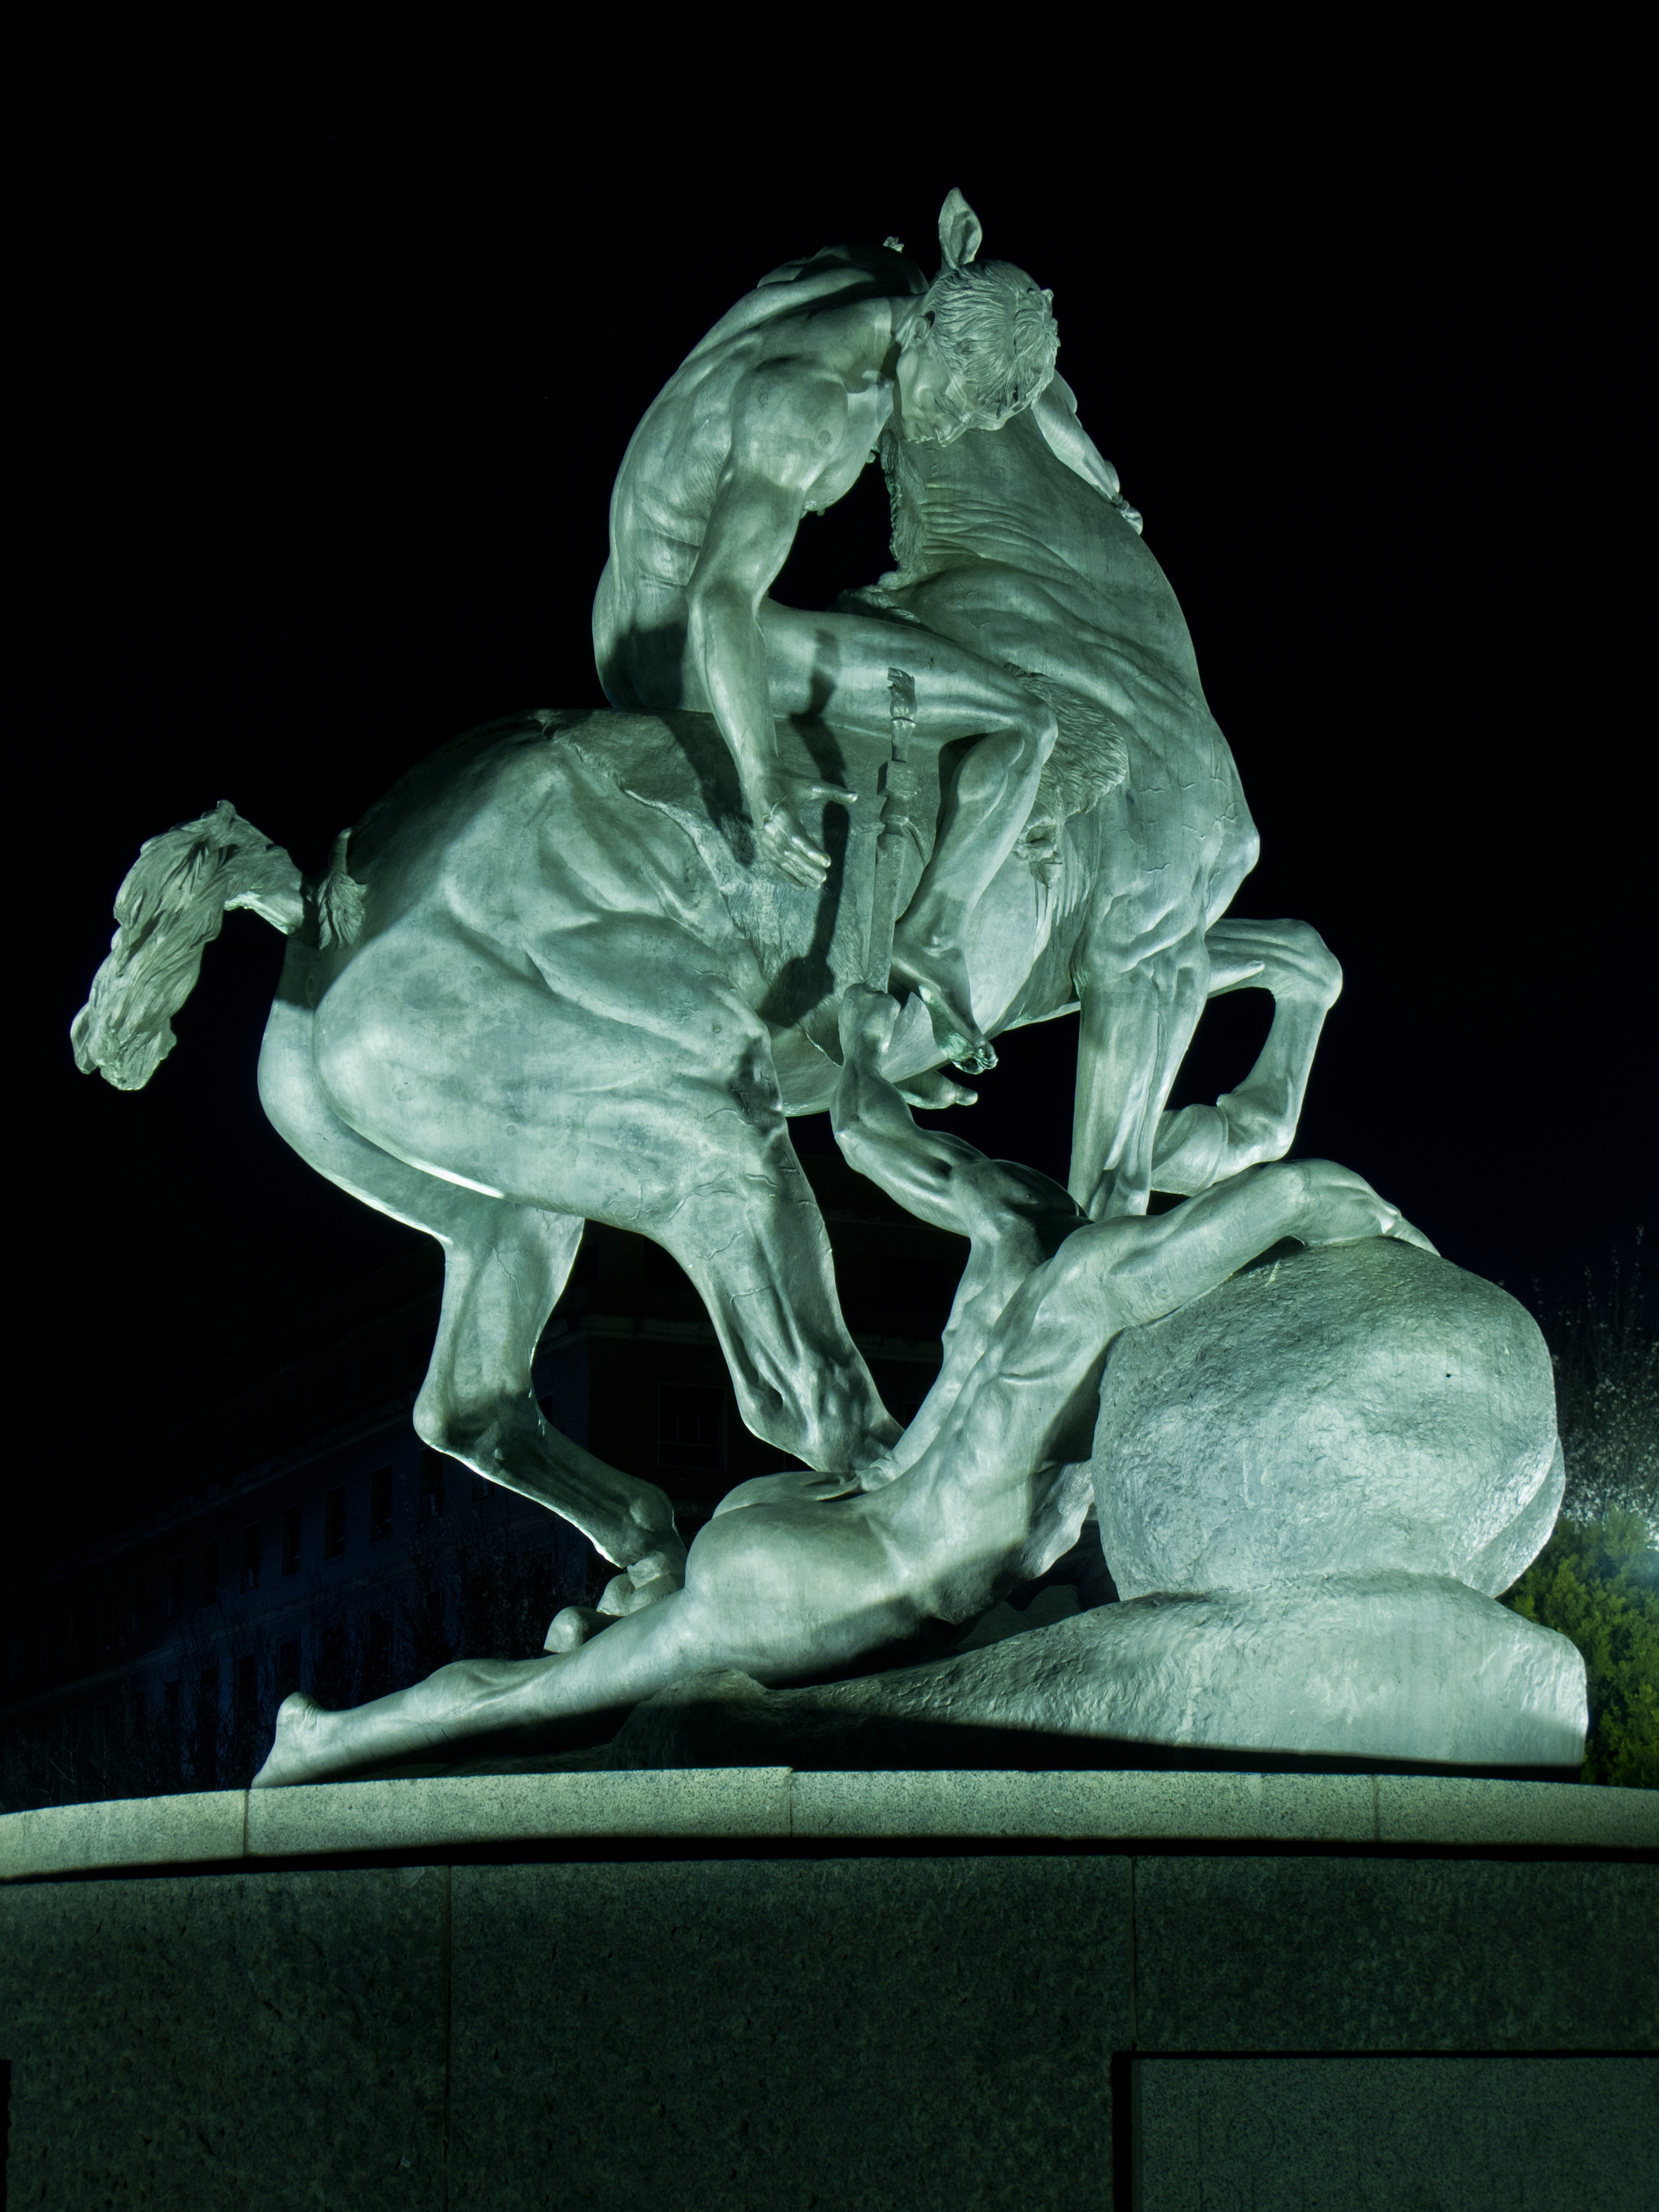
\includegraphics[width=\paperwidth]{Los_portadores_de_la_antorcha_-_05}}; % Background image
% Octavo
\node[anchor=north west,inner sep=0pt] at (0,0) {\includegraphics[width=\paperwidth]{Los_portadores_de_la_antorcha_Octavo}}; % Background image
% \node[anchor=north west,inner sep=0pt] at (0,0) {\includegraphics[width=\paperwidth]{background}}; % Background image
\draw[anchor=north] (midpoint) node [fill=ocre!30!white,fill opacity=0.6,text opacity=1,inner sep=1cm]{\LARGE\centering\bfseries\sffamily\parbox[c][][t]{\paperwidth}{\centering A Mathematical Theory of the Unknown\\ % Book title
{\large Journey Beyond the Frontiers of Human Understanding}\\[15pt] % Book subtitle
{\Large R. A. García Leiva}\\[15pt] % Author name
{\large (This book is 88\% complete)} % Disclaimer
}}; 
\end{tikzpicture}};
\end{tikzpicture}
\vfill
\endgroup

%----------------------------------------------------------------------------------------
%	COPYRIGHT PAGE
%----------------------------------------------------------------------------------------

\newpage
~\vfill
\thispagestyle{empty}

\noindent Copyright \copyright\ 2025 R. A. García Leiva % Copyright notice

\noindent \textsc{Published by the Author}\\ % Publisher


%------------------------------------------------------------------------------
%    CITA
%------------------------------------------------------------------------------

% Inserta una página en blanco
\newpage\null\thispagestyle{empty}\newpage

\newpage
\thispagestyle{empty}

\begin{quote}
\begin{flushright}
To my wife Justi, my son Daniel, \\
and my two daughters Teresa and Lucía.
\end{flushright}
\end{quote}


%----------------------------------------------------------------------------------------
%	TABLE OF CONTENTS
%----------------------------------------------------------------------------------------

\chapterimage{Platonic_cave.pdf} % Table of contents heading image

\pagestyle{empty} % No headers

\tableofcontents % Print the table of contents itself

% \listoffigures

% \listoftables

\cleardoublepage % Forces the first chapter to start on an odd page so it's on the right

\pagestyle{fancy} % Print headers again

%
% Preface
%

%
% Preface
%

\chapterimage{Ramon_Llull_-_Ars_Magna_Fig_1.pdf} % Chapter heading image

\chapter*{Preface}

\begin{quote}
\begin{flushright}
\emph{Perfection is achieved not when there is nothing more to add, \\
but when there is nothing left to take away.}\\
Antoine de Saint-Exupéry\\
\end{flushright}
\end{quote}
\bigskip

% An explanation of the main assumption behind the book

The core premise of this book asserts that perfect knowledge implies randomness. This notion may seem highly counterintuitive at first glance, given that much of scientific endeavor focuses on naming, organizing, and classifying our intricate and chaotic world. It would appear that science is anything but random. However, that is not the case.

A lengthy explanation of a scientific concept often indicates an incomplete understanding. The calculus of derivatives serves as a fitting example. In the era of Newton and Leibniz, comprehending the concept of a function's derivative necessitated substantial space for definition and was grasped only by a select group of specialists. In contrast, today's definition of derivative is concisely explained in a single paragraph and taught in high schools.

Long explanations tend to be superfluous, filled with redundancies, extraneous concepts, improperly identified relationships, and poor notation. As our understanding deepens, often through extensive research, we can eliminate the unnecessary elements from theories, eventually achieving a state of perfect knowledge. When a theory is perfect and nothing remains to be removed, its description becomes an incompressible string, which aligns with the mathematical definition of a random string - an incompressible sequence of symbols. A scientific theory is deemed random when it encompasses the maximum amount of information within the smallest possible space.

Far from being an obstacle, the limitations that randomness imposes on our knowledge unlock up new possibilities in science and technology. By comprehending these limitations, we can address the most challenging open problems and discover fascinating new research questions.

This book introduces the new "Theory of Nescience," a mathematical framework that reexamines the nature of science and the acquisition of scientific knowledge. We begin with the assumption that it is easier to measure our ignorance than to quantify our understanding, as randomness sets the ultimate boundary on our knowledge. We also posit that the computer, as a conceptual model, is the ideal tool to measure this elusive quantity. The book also explores the practical applications of the theory of nescience in scientific research, artificial intelligence, computational creativity, and software engineering.

%
% Section: Research Agenda
%

\subsection*{Research Agenda}

In this section we present a comprehensive list of research questions that aim to address critical gaps in our current understanding of science and the scientific method. With the objective of fostering intellectual curiosity and scientific progress, our interdisciplinary approach will bring together knowledge from multiple and diverse fields, combining their unique perspectives and methods. In pursuit of answers to these pressing questions, we aim to expand the boundaries of human understanding and contribute to the development of innovative solutions that have the potential to transform our society and the world around us.

\emph{Q1: Can we provide a quantitative characterization of our ignorance regarding a research topic?} Utilizing this metric would enable us to not only gauge the extent of our lack of knowledge on a specific subject, such as climate change, but also to measure the degree to which a new development or idea (typically published in a research paper) contributes to enhancing our understanding. By combining this metric with an assessment of the problem's relevance, we could effectively quantify the value of new scientific contributions.

\emph{Q2: Can we compare the extent of our ignorance across disparate scientific fields?} If feasible, this would enable us to classify and compare all open questions based on the extent of our lack of knowledge, independent of the disciplines they belong to (e.g., physics, biology, sociology). Coupling this classification with the previously mentioned relevance metric would allow us to determine where to focus our research efforts. It is important to note that this proposal does not suggest ceasing research in basic or fundamental science; on the contrary, it underscores the necessity of such inquiries.

\emph{Q3: How can we differentiate between science and pseudo-science?} This enduring and unresolved question in the philosophy of science has significant implications. Developing a practical, mathematically-based solution would be highly beneficial, as it would enable us to evaluate the scientific nature of various controversial disciplines that claim to be scientific.

\emph{Q4: Do some research topics inherently possess a higher degree of complexity than others?} Addressing this question would help determine whether researchers in certain disciplines are genuinely more intellectually adept than their counterparts in other fields, as they often claim, or if the perceived difference is merely a consequence of some subjects being easier to comprehend than others.

\emph{Q5: Are there research topics beyond the scope of human comprehension?} What are the boundaries of human understanding? It is possible that certain problems may be unsolvable by humans, and some research topics could be beyond the grasp of our limited cognitive abilities. It might be necessary to accept that progress in specific research areas can only be achieved by relinquishing control and allowing computers to perform the creative scientific work.

\emph{Q6: Can we establish a systematic procedure to enhance our knowledge?} It is possible that the so-called "scientific method" represents an unsolvable problem, with only practical approximations available to us. If this is the case, how can we evaluate and compare different approximations? Could the principles of the theory of nescience be employed to develop a novel and more effective method for expanding our understanding?

\emph{Q7: What effort is required to fully comprehend an unfamiliar subject?} For instance, what would be the cost of increasing our understanding of cancer treatment by 1\%? With such a metric, we could strategize our research activities based on priorities, budget, and the significance of potential outcomes. Naturally, this metric would represent a lower bound, as the actual effort could be greater due to factors such as poor project management.

\emph{Q8: What constitutes perfect knowledge? Is perfect knowledge attainable for all possible entities?} Randomness serves as a necessary condition for perfect knowledge, but additional criteria are required to fully define complete understanding. Furthermore, it is essential to determine whether perfect knowledge is universally achievable or if there are inherent limitations that render perfection in science an unattainable ideal.

\emph{Q9: Can we devise a method for discovering new, previously unknown, and intriguing research entities and problems?} A procedure is needed to explore the unknown unknowns—problems that we not only lack solutions for but are also unaware of their existence. Such a method could enable us to uncover future research topics and bring them to the forefront of current investigation.

Some responses presented in this book are more developed than others. For certain questions, we will provide a comprehensive theoretical answer accompanied by a practical implementation, while for others, we will offer only a rough outline of a potential solution. However, we are confident that with further research, the new theory of nescience can yield satisfactory answers to all the questions posed. In this regard, this book serves more as a research agenda rather than a complete description of a fully-developed theory of nescience.

%
% Section: Origins of the Theory of Nescience
%

\subsection*{Origins of the Theory of Nescience}

I think it was in 1991 (when I was eighteen) that I read for the first time the sentence \emph{"Computers are useless, they can only give you answers"}. The quote is attributed to Pablo Picasso, one of the most creative and influential artists of the 20th century. Soon I realized how terrible right he was, since it is true that computers cannot make interesting, original, questions. But it was more than 20 years later, in 2014, when I started to look seriously to the challenge that Picasso posed to the computer science community.

Most of the concepts behind my methodology for the discovery of interesting questions were formulated in just one night that I could not sleep: nescience, relevance, unknown unknown, and many others. Or perhaps they were developed by my subconscious mind during all those 20 years, since I do not think it was a matter of luck that I decided to pursue subjects like information theory or Kolmogorov complexity long before I was aware that they were the foundation of a future theory of nescience. What it is remarkable is that it took me just one single night to come up with a rough sketch of the most important ideas, a couple of months to develop the initial computer experiments that validated them, and several years to fully develop the mathematics needed to provide the theoretical support.

At the beginning, I was mostly interested in finding interesting scientific questions, that is, to discover what it is hidden in what I call the unknown unknown area, with the aim of bringing to the present the research topics of the future. Later on I started to look into the evolution of the nescience of scientific topics over time, and I asked myself what would happen if we keep improving a theory forever. It is then when I realized that perfect knowledge implies randomness, and the original methodology for the discovery of interesting questions was extended into a full theory of nescience to develop this important idea.

I may confess that the new theory has had, in general, a pleasant welcome form my colleges and those scientists to whom I had the opportunity to talk during the initial development stages. This early success encouraged me to continue with a further improvement of the main ideas and their applications in practice. Meanwhile I was developing the mathematics supporting the concept of nescience, I started to look into other potential applications, including the analysis of computer programs (quality assurance) and raw datasets (machine learning).

{\color{red} TODO: Remove the following paragraph if at the end these results are not included in this version of the book.}

However, I was not satisfied with the status of the theory in spite of its explanatory power. It is true that given the theory I was able to provide solutions to some open questions in the area of philosophy of science, for example, how well we understand mathematics compared to sociology, why some research topics are more difficult that others, what it is the fundamental difference between science and pseudoscience, and many others. But the problem was that the theory did not provide any predictions that could be falsified by means of running an experiment. So I decided to take the risk and further develop the mathematics to provide such kind of predictions. This is when I came up with the function that describes how nescience decreases as we increase our research effort. This function allows us to predict the maximum increment of knowledge that we can gather about a topic given the amount of effort we are willing to put in its understanding. But, still not fully satisfied, I decided to push the theory one step forward and try to find a novel prediction, that is, something that had not been observed before. New developments of the mathematical foundations behind the theory allowed me to discover the highly counterintuitive property that sometimes, for a certain class of topics, further research could be a counterproductive activity. That is, that more research we do, the more confused we get, since for these topics it is not possible to increase our knowledge beyond a critical point, even if this point if far from a perfect knowledge.

%
% Section: About the book
%

\subsubsection*{About the Book}

The theory of nescience borrows concepts from multiple academic disciplines: computability, randomness, information theory, complexity, probability, graph theory, philosophy of science, and many more. However, the book is self-contained, and so, no previous knowledge is required to follow the mathematical developments, beyond familiarity with first year calculus, abstract algebra and some computer programming experience. The contents have been selected to cover the needs of readers with very different backgrounds: mathematicians, computer scientists, engineers, ... The math level is that of a graduate student or advanced undergraduate.

{\color{red} TODO: Review and update once the book is finished.}

The book has been structured into three main parts: Background, Foundations and Applications. Readers already familiar with the mathematics covered by the Background section can directly proceed to the Foundations part. However, it is highly recommended to perform at least a quick review of the notation used in these chapters. After getting acquainted with the details of the theory of nescience described in the Foundations section, the reader can continue with the applications. It is not necessary to fully understand all the details of the theory in order to follow the applications. A basic knowledge of the main concepts and results should be sufficient.

\bigskip

\begin{itemize}

\item \emph{Chapter \ref{chap:Introduction} Introduction} contains a gentle introduction to the theory of nescience, and a short review of the main results. The chapter avoids the use of advanced mathematics, but the concepts are still semi-formally introduced. Although it is not recommended, those readers that cannot follow the mathematics behind the theory could just read this first chapter, the introductory sections of the remaining chapters of the Background and Foundations parts, and then proceed directly to the applications.

\end{itemize}

\bigskip

\emph{PART I Background} is an introduction to the mathematics required to measure how much we do not know about a topic and how random is a string. The goal of this part is to fix notation, formally define concepts, and prove some important results. I do not assume any previous knowledge to follow the covered material, however, to fully understand these topics I recommend to refer to the standard literature (see the References section included at the end of each chapter). Addtional topics are covered in the appendices.

\begin{itemize}

\item \emph{Chapter \ref{chap:Discrete_Mathematics} Discrete Mathematics} is an overview of the basic mathematics required to understand the more advanced topics covered in the book. This chapter is intended as a quick review of these concepts, and so, no formal definitions are provided and theorems are not proved. Among others, the topics covered include sets, relations, strings, graphs and discrete probability.
 
\item \emph{Chapter \ref Discre Probability} {\color{red} TODO}.

\item \emph{Chapter \ref{chap:Computability} Computability} provides a formal definition of the concept of algorithm. We will introduce the concept of universal Turing machine, and we will see that there are well defined mathematical problems that cannot be solved by computers. The very important tools of oracle Turing machine and Turing reducibility are also studied in detail. Computational complexity main results are briefly reviewed.

\item In \emph{Chapter \ref{chap:Coding} Coding} we will study the properties of codes, and in particular, how codes allow us to compress a text without loosing any information by means of removing statistical redundancy. We will see that there exists a limit to how much a text can be compressed by using this technique, and that this limit is given by the entropy of the source.

\item \emph{Chapter \ref{chap:Algorithmic_Information} Complexity} introduces an absolute metric, called Kolmogorov complexity, to measure the amount of information contained in a string, by computing the length of the shortest computer program that can print that string. The properties of this metric are studied in detail. The relation between string complexity and randomness is also discussed.

\item \emph{Chapter \ref{ch:Learning} Learning} studies the relation between codes and probabilities. It provides a short review of the area of statistical learning, with a focus on existing approaches that apply the concept of minimum string length to the problem of stochastic models evaluation and optimal parameters selection. An introduction to the concepts and notation of nonlinear multiobjective optimization problems is included as well. 

\item \emph{Chapter \ref{chap:Philosophy} Philosophy of Science} is a short introduction to the discipline of philosophy of science. We will review concepts like scientific representations, models, theories and many other components of science from a philosophical point of view, identifying the most important elements that any formal theory of science should include. The chapter also contains a review of the current state of the art of what it is the scientific method.

\end{itemize}

\bigskip

\emph{PART II Foundations} contains a detailed description of the theory of nescience, defining formally the concepts involved and proving the main theoretical results. This is the most important part of the book, where the new theory is fully developed. Readers with a solid background in computability, complexity, information theory and probability could proceed directly to this part.

\begin{itemize}

\item \emph{Chapter \ref{cha:Topics-and-Descriptions} Entities, Representations and Descriptions} introduces the basic constituents of the theory of nescience: entities, representations and descriptions. The properties of these elements and how they interlace together are studied. We will see how multiple representations and descriptions can be combined, and how to include background knowledge in a research. The relation between perfect knowledge and randomness is discussed, and a novel concept of research area is proposed.

\item \emph{Chapter \ref{chap:Miscoding} Miscoding} address the difficult problem of how to represent abstract, and non-abstract, research entities as string of symbols that can be used for research. In the chapter we will formally introduce the concept of miscoding and study its properties. Miscoding is a quantity that measures the error introduced due to improper encodings.

\item \emph{Chapter \ref{chap:Error} Inaccuracy} contains a novel interpretation of the classical concept of error, that is, how accurately a description explains an entity. The concept of inaccuracy is extended to deal with all kinds of topics, including abstract ones. The joint and conditional versions of the concept of inaccuracy are introduced and their properties studied.

\item \emph{Chapter \ref{chap:Redundancy} Surfeit} studies how redundant is a description, that is, how many unnecessary elements a description contains. Surfeit can be seen as a measure of how well we currently understand research topics and research areas. The joint and conditional versions of surfeit are provided as well.

\item \emph{Chapter \ref{chap:Nescience} Nescience} is the central chapter of the book, since it contains the mathematical foundations of the new theory. In the chapter is formally defined the concept of nescience and its main properties studied, like for example, how nescience evolves with time, what we mean by perfect knowledge, and how to identified our current best model.

\item \emph{Chapter \ref{chap:Interesting-Research-Questions} Interesting Questions} describes a procedure to find new interesting things in a large collection of measurable objects, and in particular, to find new interesting research questions and new research topics. New concepts like relevance and applicability are defined and studied.

\item \emph{Chapter \ref{chap:Properties-Nescience} Advanced Properties} covers some advanced concepts and properties of the theory of nescience. These properties are not needed to understand the applications of the theory, and so, they can be safely skipped in a first read of the book (but, definitely, not in a second). Among others, new concepts introduced include: an axiomatic version of the theory, graspness as a measure of how difficult is a particular research topic, or the minimum effort required to reduce the nescience of a topic.

\end{itemize}

\bigskip

\emph{PART III Applications} provides a collection of practical applications of the concept of nescience, in the areas of machine learning, software engineering, philosophy of science, and computational creativity. The applications have been selected to cover the entire spectrum of possible kinds of topics, from abstract ones (research topics), real objects and strings (computer programs).

\begin{itemize}

\item \emph{Chapter \ref{chap:Machine-Learning} Machine Learning} describes how the concept of nescience can be applied in the case of entities represented by large datasets. In particular, the methodology will be applied to select relevant features, identify optimal models, and compute errors. Some new machine learning algorithms, like a novel approach to derive optimal decision trees, will be proposed as well.

\item \emph{Chapter \ref{chap:Software-Engineering} Software Engineering} covers how to use the theory of nescience with computer programs, in order to provide a measure of how well we understand current software platforms (operating systems, networking middleware, productivity tools, ...). We will evaluate if current versions of software are better than past versions, or if software is degrading with time. The results are also applied to the automatic discovery of errors, with the aim to improve the quality of software.

\item \emph{Chapter \ref{chap:philosophy-science} Philosophy of Science} studies how to apply the new metrics introduced in this book to study of what it is science and how science is made. Some important open problems in the area of philosophy of science will be addressed, including the demarcation problem (how to distinguish between science from pseudoscience) and the question of how science make progress. Multiple proposals of what it is the scientific method are evaluated in the context of the theory of nescience, and compared against our own proposal.

\item \emph{Chapter \ref{chap:computational-creativity} Computational Creativity} shows how to apply in practice the methodology for the discovery of interesting things. In particular, the methodology will be applied to find new research questions and new research topics, where multiple examples of interesting questions and topics will be provided.

\end{itemize}

\bigskip

\emph{Appendix \ref{apx:foundations_mathematics} Foundations of Mathematics} describes three different theoretical frameworks from which mathematics can be formalized: logic and set theory, dependent type theory, and category theory. These frameworks can also be used to provide a solid foundation to the theory of nescience.

\emph{Appendix \ref{apx:math} Advanced Mathematics} contains a brief description of some mathematical concepts that have been used in the book, but that play a secondary role in the development of the theory; they are included in this appendix for reference.

\emph{Appendix \ref{apx:coq} Mechanical Proofs} provides a mechanical implementation of the axioms of the theory of nescience, and its most relevant results, based on the calculus of inductive constructions, and in particular, in the \texttt{Coq} proof assistant.

Last, but not least, \emph{Appendix \ref{apx:photos} About the Photos} explains the origin and intended meaning of the carefully selected photographs included at the header of each chapter.

%
% Section: Acknowledgements
%

\section*{Acknowledgements}

I would like to give thanks to all the people who has contributed with comments and ideas to the development of the theory of nescience. In particular, I would like to give thanks to Antonio Fernández, Vincenzo Mancuso and Paolo Casari who believed and supported this project since its very beginning, when it was only a crazy nonsense idea (although perhaps it still is). Other people who has provided contributions and useful comments where Héctor Cordobés, Luis F. Chiroque, Agustín Santos, Marco Ajmone, Pablo Rojo, Manuel Cebrián, Andrés Ortega, Emilio Amaya, Mattis Choummanivong, Alexander Lynch, Andrés Carrillo and Simon Bihoreau. The \texttt{fastautoml} library described in Chapter \ref{chap:Machine-Learning} has been partially funded by the IMDEA Networks Institute, the European Union's Horizon 2020 research and innovation programme under grant agreement No 732667 RECAP, and Nokia Spain through the project NetPredict.

Finally, I would like to give thanks to my parents who gave me the opportunities in life they didn't have, and to my wife and my three kids who provide ultimate meaning to my life.

%
% Section: Disclaimer
%

\section*{Disclaimer}

I would like to leave it clear that the overwhelming majority of the ideas contained in this book are not mine. The intuition comes form the great minds of our history: Occam, Llull, Leibniz, Newton, etc., and from philosophers like Plato, Popper, Feyerabend, Wittgenstein, etc. Also, I have leveraged on the mathematical theories developed by scientists like Turing, Church, Post, Shannon, Solomonof, Chaitin, Kolmogorov, and many others. My only original contribution with this book is that I have, perhaps, connected some dots, and that I have provided a, perhaps, interesting reinterpretation of some old ideas. In the References sections included at the end of each chapter there is a description of the works I have used to write the book. In the text I use passive voice ("it is defined") whenever I know that a concept is not mine, and active voice ("we define") when I am not aware of a previous use of this concept by somebody else.



%
% CHAPTER: Introduction
%

%
% Introduction
%

\chapterimage{Galileos-telescope-002.pdf} % Chapter heading image

\chapter{Introduction}
\label{chap:Introduction}

\begin{quote}
\begin{flushright}
\emph{If presented with a choice between indifferent alternatives,\\
then one ought to select the simplest one.}\\
Occam’s razor principle 
\end{flushright}
\end{quote}
\bigskip

The quest for knowledge usually starts by identifying a set of entities we would like to understand. The elements of this set can be almost anything. If we are mathematicians, our set of interest will be composed by mathematical concepts; if we are biologists, the set will be living things; and if we are engineers, it will be machines that solve problems. Our goal, as researchers, is to understand as much as possible about those entities. We want to understand how things work because that allows us to forecast the consequences of our actions. For example, we know that if we apply a sufficient amount of heat to a pile of wood, a fire will start. Also, and more challenging, looking at consequences we can try to infer the causes; if I have fever, maybe I have been infected by a virus. Understanding is how we solve problems in practice, and understanding means to find patterns or regularities that allows us to build a simplified description, or model, of the original entities so we can manipulate them to our convenience.

Ideally, we would like that given our descriptions we should be able to reconstruct the original entities under study. However, for the majority of entities this is not possible, like for example with the abstract ones. Instead, what we have to do is to work with representations, that is, use texts or data that try to capture as many details of the original entities as possible. If we are physicists the representation of an entity could be the result of an experiment, if we are computer scientists it could be a dataset composed by measurements, or if we are sociologists what we might have is a collection of observed facts. In Figure \ref{fig:representationProblem} it is depicted this process: we would like our descriptions to model entities, but what they model is our artificial representation of those entities.

\begin{figure}[h]
\centering\includegraphics[scale=0.5]{representationProblem}
\caption{\label{fig:representationProblem}The Problem of Understanding.}
\end{figure}

The question is how well our descriptions explain the original entities through the modeling of the representations that encode those entities. There are multiple sources of error we should consider. The first one is that our encoding method might not be perfect. That is, if the ideal representation of an entity $e$ is the string $r$, in practice we could be working with another string $r'$ that it is close to $r$, but not equal. We call this type of error \emph{miscoding}\index{Miscoding}. The second source of error is due to the fact that our descriptions are not perfect. Ideally a description $d$ should allow us to recreate the string $r'$ (the string $r$ is normally unknown), but in practice it produces another string $r''$ which is, again, close to $r'$ but not equal. This second type of error is what we call \emph{inaccuracy}\index{Inaccuracy}. Finally, the third group of errors deals with the descriptions themselves. Given the limited cognitive capabilities of humans, we are interested in the shortest possible description $d$ of $e$, so we can understand the entity, make predictions, or derive consequences. However, our current best known description $d'$ probably will be longer than $d$. This third type of error is what we call \emph{surfeit}\index{Surfeit}. Finally, we combine these three types of errors, miscoding, inaccuracy and surfeit, in a single quantity called \emph{nescience}\index{Nescience}, as a quantitative measure of how much we do not know about an entity.

This chapter contains a gentle introduction to our new \emph{theory of nescience}, and a short review of the main results of this theory. The chapter avoids the use of advanced mathematics, but concepts are still semi-formally described. Also, in order to clarify the new ideas introduced, we provide multiple practical examples.

%
% Section: Entities
%

\section{Entities}

Our theory starts by assuming there exists a non-empty collection of \emph{entities}\index{Entity}, denoted by $\mathcal{E}$, that are the subject of past, present or future scientific research. And, of course, we assume that (at least some of) these entities can be fully understood and described by science. Technically speaking $\mathcal{E}$ is not a well defined set, since the only restriction is that it must be nonempty. The abstract nature of $\mathcal{E}$ has some advantages, but also introduces important limitations. The main limitation is that our definition of nescience is, in general, a non-computable quantity, and so, it must be approximated in practice. The main advantage is that we can apply the new concepts and methods introduced in this book to other domains, not only to the discovery of solutions to open problems.

In the theory of nescience we do not allow universal sets, that is, we cannot assume the existence of a set $\mathcal{E}$ that contains everything. The problem of universal sets is that they violate Cantor's theorem\index{Cantor's theorem} (see Section \ref{sec:descriptions_entities}). Cantor's theorem states that the set $\mathcal{P}(\mathcal{E})$ composed by all the possible subsets of $\mathcal{E}$ has more elements than the original set $\mathcal{E}$, and this is a contradiction with the fact that $\mathcal{E}$ contains everything. In the theory of nescience $\mathcal{E}$ must be the set of "something". Moreover, not all possible sets are allowed. For example, the Russel's paradox\index{Russel's paradox} propose to consider the set $\mathcal{E}$ composed by all those sets that are not members of themselves; the paradox arises when we try to answer the question of whether $\mathcal{E}$ is a member of itself or not (see Section \ref{sec:descriptions_entities}). We require from every set $\mathcal{E}$ to be restricted to one particular type of elements, so they cannot be members of themselves.

Usually the set $\mathcal{E}$ corresponds to an individual domain of knowledge, and its constituent elements depend on how the theory is being applied in practice. Examples of such sets of entities could be: a collection of mathematical objects (abstract); the kingdom of animalia (living things); known and unknown human needs (abstract); all possible computer programs (strings of symbols), etc.

%
% Section: Representations
%

\section{Representations}

Most of the entities can not be the subject of a direct scientific analysis because, for example, they are abstract objects. Instead, what we have to do is to work with representations of those entities. Let $\mathcal{R_\mathcal{E}}$ be the collection of finite binary strings, called \emph{representations}\index{Representation}, that encode the entities of $\mathcal{E}$. The exact format of these strings is something that depends on the entities in which the theory of nescience is being applied. In some cases, entities will be strings themselves (e.g. computer programs), and in others they will be abstract objects that have to be encoded as strings (e.g. human needs). Note that an entity $e \in \mathcal{E}$ might have more than one valid representation in $\mathcal{R_\mathcal{E}}$. How to encode abstract entities as strings of symbols in such a way that they capture all the details and nuances of the original entities is a difficult, still unsolved, problem, and so, the set $\mathcal{R_\mathcal{E}}$ is normally unknown. 

Ideally, we would like to have an encoding function $f:\mathcal{E} \rightarrow \mathcal{R_\mathcal{E}}$ from a set of entities $\mathcal{E}$ to the set of all possible representations. Unfortunately, in practice, it is not possible to define such a function, since as we have already mentioned, the set $\mathcal{E}$ is not a well defined set, that is, we cannot tell what it is and what is not a member of this set. For example, it requires a lot more research before we can tell exactly what a human need is.

From a theoretical point of view we could take advantage of the concept of \emph{oracle Turing machine}\index{Oracle Turing machine} (see Chapter \ref{chap:Computability}) to address this problem. A Turing machine\index{Turing machine} is a mathematical model of a computer, and an oracle Turing machine is somehow like a mathematical model of a computer connected to Internet. We could assume that this computer can query an hypothetical external service, hosted somewhere in another computer, to check if a given string $r$ encodes \emph{any} entity of $\mathcal{E}$. We cannot ask the oracle if the string $r$ is a valid representation of the entity $e$ in which we are interested, because that would require to provide a valid representation of $e$ as a string of symbols, something that we cannot do since, in general, it is unknown. The concept of oracle machine allow us to define a function from the collection of finite binary strings to the set of entities $f:\mathcal{B}^\ast \rightarrow \mathcal{E}$.

From a practical point of view, we usually approximate the set $\mathcal{R}_\mathcal{E}$ by another set $\hat{\mathcal{R}}_\mathcal{E} \subseteq \mathcal{B}^\ast$ of strings that we believe are good enough representations of the entities of $\mathcal{E}$. In science, traditionally, these representations have had the form of images or drawings (e.g. biology), collection of facts (e.g. sociology), or the result of experiments (e.g. physics). Recently, and due to the huge advances in the capacity of computers to collect and store data, a new and powerful way to encode entities has emerged: the use of large collections of data as representations. Please mind that in the process of encoding we are not interested in finding the shortest possible representation of the entities, what we need is high quality representations.

We should be aware that in many practical problems, the selected representations of abstract entities will not be able to fully capture all the details of the original objects. That is, we are dealing with simplified abstractions of reality that might limit our capability of making universal statements about nature (see Chapter \ref{chap:Miscoding}).

\begin{example}
\label{ex:animals_DNA}
When the topics under study are animals (the set $\mathcal{E}$), we could use as representations a binary encoding of their DNAs (the set $\mathcal{R_\mathcal{E}}$). Although today we do not have the technology to grow a creature given its DNA, in theory it could be possible to do so. However, the DNA is not enough to fully reconstruct the original animal, since we also need to know what happened along its life. For example, what if we are dealing with a cat with only three legs because it lost one in an accident? That information is not included in its DNA. If we are interested in studying the characteristics of some species, it will be sufficient to work with the DNA of some representative sample of individuals that belongs to each species. However, if we are studying the particular individuals inside a species, we also need a way to encode the history of each animal, or a way to encode the details not covered by the DNA.
\end{example}

\begin{figure}[h]
\centering\includegraphics[scale=0.5]{entities_topics}
\caption{\label{fig:entities_topics}Entities and Representations.}
\end{figure}

A consequence of working with strings as representations (the set $\mathcal{R}_\mathcal{E}$) is that it might happen that there exist entities that are not encoded by any representation (see the gray areas in Figure \ref{fig:entities_topics}, in particular, the entity $e_3$ is not encoded by any representation). For example, if our set of entities is the set of real numbers, it turns out that there exist numbers that do not have a finite representation (we do not allow infinite strings as representations). Intuitively, we could say that for many domains of knowledge the number of problems is greater than the number of solutions. A consequence of working with approximations of representations (the set $\mathcal{R}$) is that some representations might encode the wrong entities (the representation $r_3$ in Figure \ref{fig:entities_topics}). This is due to the fact that our knowledge is incomplete, and we might be using incorrect representations for the entities of $\mathcal{E}$. Working with incomplete knowledge has an additional problem, there may be some entities whose existence we do not know yet, what we call the \emph{unknown unknown}\index{Unknown unknown}. For example, the representation $r_1$ in Figure \ref{fig:entities_topics} is not part of the set $\mathcal{R}$, and so, it is not currently considered by researchers even though it represents a valid entity $e_1$. We are interested in investigating a procedure to discover new, previously unknown, research entities from the set $\mathcal{R}_\mathcal{E}$ (see Section \ref{sec:intro_research_topics} and Chapter \ref{chap:Interesting-Research-Questions}).

A \emph{research area} $A$ is subset of topics, that is $A \subset \mathcal{R}_\mathcal{E}$. In practice, areas are useful as long as the topics included in the area share a common property. We might be interested in studying what we do not know about a particular area. For example, if the set of topics is "animals", examples of areas could be "invertebrates", "mammals", "birds", "amphibians", "reptiles" and "fish". In order to measure what we do not know about an area, first we have to provide a description of the topics included in that area. However, in general, our knowledge about the topics that compose an area is limited, and so, we can only partially describe them. Moreover, as our understanding of a research area changes, the number of topics included in its known subset changes as well. Consequently, the properties of areas can be studied only relative to our current knowledge.

\begin{example}
If our set of topics is "astronomy", a research area could be the set of "habitable planets", from which we currently known only a few of them. A model of this area would be a description of those already known habitable planets.
\end{example}

%
% Section: Descriptions
%

\section{Descriptions}

Once we have identified the set $\mathcal{R}$ of possible representations, we have to provide a way to describe them, that is, to formulate our theories or models about how things work. As humans, we have very limited cognitive capabilities, and so, we rely in the use of simple models of nature in order to understand observed facts, and to forecast the results of our own actions. 

What constitutes a valid description of an entity is a difficult, still unsolved, problem. For example, the Berry paradox\index{Berry paradox} proposes the following description "the smallest positive integer not describable in fewer than twelve words". The paradox arises because we have just described this number with only eleven words. In order to avoid these kind of paradoxes, in the theory of nescience we require that a description for an entity must be a finite string of symbols from which we can fully and effectively reconstruct one of the possible representations of the original entity. By "effectively reconstruct" we mean that our models must be computer programs that when executed they print the selected representation. Since Newton, science is about mathematical models, that is, the search of a set of functions that fully describe the objects found in Nature and their relations. In the theory of nescience we go one step beyond and require that those models must be computable.

Descriptions\index{Description} are composed by two parts, a Turing machine\index{Turing machine} $TM$ (a computer program) that implements all the regularities found in the entity's representation (the compressible part), and an input string $a$ to this program that contains a literal description of what is left (the non-compressible part). From a formal point of view, a description for a representation $r \in \mathcal{R}$ is a string $\langle TM, a \rangle$ such that $TM(a) = r$. This two part nature of descriptions somehow resembles our classical distinction between theories and assumptions, theories and initial conditions, problems and particular instances of problems, species and individuals, etc. For example, a description could be composed by a set of differential equations modeling a system (the compressible part), and the collection of initial conditions (the non-compressible part). The actual interpretation of the pair $\langle TM, a \rangle$ is something that depends on the particular details of the set of entities in which that theory is being applied.

\begin{figure}[h]
\centering\includegraphics[scale=0.5]{entities_topics_models}
\caption{\label{fig:entities_topics_models}Entities, representations and descriptions.}
\end{figure}

In Figure \ref{fig:entities_topics_models} it is shown graphically the relation between entities, representations and descriptions (the set of all possible descriptions is denoted by $\mathcal{D}$). Not every possible string is a description, since we require that a descriptions must be based on Turing machines, and not all possible descriptions describe valid representations.

\begin{example}
From an intuitive point of view, if we are studying how our world works, from a physical macroscopic point of view, our set of possible descriptions would include, among others, the following elements: Aristotelian physics, Cartesian physics, Newtonian physics, Einstein's theory of general relativity and superstring theory. Our current best description would be  Einstein's theory of general relativity (superstring theory has not been validated experimentally yet).
\end{example}

A representation $r \in \mathcal{R}$ can have multiple descriptions, and so, the goal of science is to find the shortest possible description, denoted by $d^\star$, that allows us to fully reconstruct the representation $r$. Unfortunately, there does not exist a method or algorithm that given a string, returns the shortest possible computer program that prints that string (see the result of incomputability of Kolmogorov complexity in Chapter \ref{chap:Algorithmic_Information}). In particular, there does not exist a method that given a representation finds the shortest possible description. That is, science is a non-computable problem and so, we have to find a collection of heuristics that allow us to approximate the optimal solution. This collection of heuristics is what we call a \emph{scientific method}\index{Scientific method}.

In the theory of nescience we are interested in understanding, and quantitatively measuring, what can be wrong in the ideal process depicted in Figure \ref{fig:entities_topics_models}. In Sections \ref{sec:ch1_miscoding}, \ref{sec:introduction:inaccuracy}, and \ref{sec:ch1_surfeit} we will propose a collection of metrics to measure each possible source of error, and in Section \ref{sec:ch1_nescience} we will see how to combine all these concepts into a single quantity, called \emph{nescience}. The new metric of nescience allow us to quantitatively measure how much we do not know about a research entity.

%
% Section: Miscoding
%

\section{Miscoding}
\label{sec:ch1_miscoding}

As we have seen, for the majority of the scientific disciplines, the set $\mathcal{E}$ of entities under consideration could be composed by abstract elements, or other kind of objects that are not easily represented as a string of symbols. Also, it might happen that our current understanding of the elements of $\mathcal{E}$ is limited, and so, we can not properly encode them. In those cases we have to work with approximate representations instead of the valid representations. We are interested in knowing the error introduced due to the use of these incorrect representations.

\begin{figure}[h]
\centering\includegraphics[scale=0.5]{miscoding}
\caption{\label{fig:miscoding}Miscoding of topics.}
\end{figure}

We propose to quantify the \emph{miscoding}\index{Miscoding} of an incorrect representation $r'$ as the length of the shortest computer program that can print the correct representation $r$ having as input $r'$, denoted by $K(r|r')$. See Figure \ref{fig:miscoding}, where $\mathcal{R}_e$ denotes the set of strings that correctly represent the entity $e$. Intuitively, miscoding measures the effort (measured as the length of a program, not as the time it takes to that program to do its work) required to fix the incorrect representation. For example, if our representation contains some errors, the program should be able to identify and correct those errors; or if our representation is missing some critical information required to fully encode the entity, the program will contain, hard-wired, that missing information.

However this approach is not sufficient to fully capture our intuitive notion of miscoding. The problem arises when our represenation $r'$ contains additional information that is not needed to encode the entity $e$. In this case, it might happen that our descriptions include elements modeling those unnecessary symbols, making them artificially long. For example, in a experiment we could be measuring features that do not influence at all the result of the experiment, and given our limited understanding of the original entity, our current description could include those features as predictors\footnote{\color{red} TODO: This example is confusing, since the experiment describes a cause-effect situation, and our machine learning algorithm could identify non-relevant features authomatically. Use a different example.}. In order to avoid this problem, we have to compute also the length of the shortest computer program that can print the incorrect description $r'$ having as input the correct one $r$, that is, $K(r'|r)$. Then, miscoding could be defined as the maximum of these two lengths $\max\{ K(r \mid r'), K(r' \mid r)\}$.

Unfortunately, this last definition still presents some practical problems. Most of the entities have multiple valid representations. Maybe $r'$ is far from a representation $r_1$, but it is closer to a second one $r_2$. It would be unfair to say that a description $d$ that perfectly model $r_2$ is a bad descriptions because it does not model $r_1$, since both, $r_1$ and $r_2$ represent the same entity $e$. A possible solution to this problem would be to look at $\min_{r \in \mathcal{R}_e} \{ \max\{ K(r \mid r'), K(r' \mid r)\} \}$.

\begin{example}
\label{ex:leibnez-wallis}
Let $e$ be the abstract entity called "Pi constant", that is, the ratio of a circle's circumference to its diameter; let $r$ be the Wallis' product\index{Wallis' product} $2 (\frac{2}{1} \cdot \frac{2}{3} \cdot \frac{4}{3} \cdot \frac{4}{5} \cdot \frac{6}{5} \cdot \ldots)$, one of the valid representations of $e$; and let $d$ be the description $\sum_{n=0}^\infty \frac{(-1)^n}{2n+1}$. It would be unfair to affirm that $d$ is a terribly bad description for the entity $e$ because it does not print $r$. In fact, $d$ produces the Leibniz's series\index{Leibniz's series} $4 (1 - \frac{1}{3} + \frac{1}{5} - \frac{1}{7} + \ldots)$ that it is also a valid representation of Pi. Leibniz's series should not be classified as a miscoded representation of Pi, even in the hypothetical case that it were unknown by mathematicians.
\end{example}

As example \ref{ex:leibnez-wallis} pointed it out, one of the most difficult problems with the definition of miscoding is that the set $\mathcal{R}_e$ of valid representations for the entity $e$ is, in general, not known. From a theoretical point of view we could resort again to the oracle Turing machine\index{Oracle Turing machine} to address this problem. However, as we have seen, we cannot ask the oracle if the string $r$ is a valid representation of the entity $e$ in which we are interested (the set $\mathcal{R}_e$), since that would require to provide a valid representation of $e$ as a string of symbols, something that, in general, cannot be done. The only thing we can do is to ask the oracle how far the string $r$ is from being a valid representation of any entity from the set of entities $\mathcal{R}_\mathcal{E}$.

Taking into account all the above considerations, we define the miscoding of a representation $r$, denoted by $\mu(r)$, as:
\[
\mu(r) = \overset{o}{ \underset{r_e \in \mathcal{R}_\mathcal{E}} \min} \frac{ \max\{ K(r_e \mid r), K(r \mid r_e) \} } { \max\{ K(r_e), K(r) \} }
\]
where $\overset{o} \min$ means that the minimum function has to be computed by an oracle. Note that in the definition we have introduced the normalization factor $K(r_e)$, that is, the length of the shortest program that can print $r_e$, because we are interested in comparing the miscoding of multiple, possibly unrelated, representations.

Since miscoding does not take as argument the original entity $e$, it may be the case that what we are representing is not what we were expecting. That is, with our representations and descriptions we might be studying a different entity. This is something that happens quite often in the practice of scientific research. 

\begin{example}
At the end of the eighteenth century, the chemist Joseph Priestley thought he was studying the nonexistent entity called "phlogiston"\index{Phlogiston}, a fire-like element that was supposed to be contained within combustible bodies and released during combustion. It turned out that he was studying a completely different entity called "oxygen".
\end{example}

According to the theory of nescience, our task as researchers is not only to find the proper representations of the entities of $\mathcal{E}$, but also to discover how this ideal oracle machine that knows how to properly encode entities works. That is, why our representations constitute good encodings of the entities under study.

%
% Section: Inaccuracy
%

\section{Inaccuracy}
\label{sec:introduction:inaccuracy}

In the previous section we have characterized how much we do not know about an entity $e$ in terms of the miscoding due to using a wrong representation $r'$ instead of a correct one $r$. In this section we are interested in how much we do not know given a description. Ideally we should be working with a description $d$ that allows us to fully reconstruct the representation $r'$ (recall that the representation $r$ might be unknown), but in general this is not the case in practice. Normally we will be working with a description $d'$ that prints out a string $r''$ (remember that we require that descriptions must be computer programs) that it is (hopefully) close to the string $r'$, but not equal. In this case we say that the description $d'$ is an \emph{inaccurate} description of the representation $r'$ (see Figure \ref{fig:inaccuracy:inaccuracy:inaccuracy}).

\begin{figure}[h]
\centering\includegraphics[scale=0.5]{inaccuracy}
\caption{\label{fig:inaccuracy:inaccuracy:inaccuracy}Inaccuracy of a description.}
\end{figure}

If a description is inaccurate for a representation, we would like to have a quantitative measure of how far we are from properly modeling the representation. A natural way to define this measure would be by means of computing the effort required to fix the output of our inaccurate description. In this sense, inaccuracy could be given by the length of the shortest computer program that can print the representation given as input the wrong representation produced by the description. However, as it was the case of miscoding, in order to have a complete picture of the error made with the description $d$ we have to compute also how difficult is to print the inaccurate representation given the good one. It might happen that our description $d$ is modeling things that have nothing to do with the representation $r'$, and simply ignoring those elements is not a solution.

Let $r' \in \mathcal{R}$ be a representation, and $d \in \mathcal{D}$ a description that produces the string $r''$; we define the \emph{inaccuracy}\index{Inaccuracy} of the description $d$ for the representation $r'$, denoted by $\iota(d, r')$, as:
\[
\iota(d, r') = \frac{ \max\{ K(r'' \mid r'), K(r' \mid r'') \} } { \max\{ K(r'), K(r'') \} }
\]
Again, since what we need is the broadest possible interpretation of the concept of inaccuracy, we have to divide by the normalization factor $\max\{ K(r'), K(r'') \}$, so we can compare multiple descriptions for the same representation as well as descriptions for different representations.

We prefer the term \emph{inaccuracy} over the term \emph{error}. Error is given by two components, precision and accuracy. But precision mostly refers to continuous systems, and since we are dealing with discrete strings of symbols, it does not make too much sense to talk about precision in this context.

In practice it is a difficult task to compute the inaccuracy associated with the description of a representation, since, as we have already said, finding the length of the shortest computer program that can print a string is a non-computable problem. If the original entities are texts themselves, the inaccuracy could be approximated using compression algorithms, where the Kolmogorov complexity is approximated with the length of the compressed text using a compressor. If topics are abstract entities, like mathematical concepts, their descriptions could be based on the result of an experiment, and so, the inaccuracy could be based on the error of the model (for example, by means of computing the length of the additional information required to fully describe the results of the experiment given the model). In this sense, our definition of inaccuracy is a generalization of the concept of error, since it can be applied to multiple types of entities, not only to those entities that can be encoded as datasets.

\begin{example}
\label{ex:introduction:inaccuracy:newton}
{\color{red} TODO: Review this example.}
The topic Newton's second law\index{Newton's second law} of motion $F = m a$ could be encoded given the results of an experiment using objects of different masses to which we apply different forces and then we measure the acceleration. The dataset would be composed by the masses, the forces, and the accelerations achieved for each combination of mass and force. However, if we are interested in the acceleration due to gravity, forces and masses cancel out, and so, the only value to measure is acceleration.  Of course, if the result of the experiment is a large collection of measurements, the encoding of the entity would be very long. But, as we said before, with the encodings of entities we are not interested in finding the shortest possible strings, what we are looking for are complete and accurate encodings of topics. For this example we will use the results of an experiment performed by the National Bureau of Standards in Washington D.C. between May 1934 and July 1935. The dataset is composed by 81 measurements, and each value is expressed in centimeters per second squared, for example 980,078. In practice we approximate the quantity $\frac{ K(t \mid m) } {K(t)}$ by $\frac{ C(D \mid M) } {l(D)}$, where $C(D \mid M)$ is the length of the compressed version of the data given the model (using a standard compressor), and $C(D)$ is the length of the compressed data. In order to encode the dataset we require 20 bits per measure (using an uniform code, as it is explained in Chapter \ref{chap:Coding}), and so, to encode the full dataset we require 1,620 bits. If we assume that our model predicts a gravity of $980,000 cm/s^2$ plus a random error that follows a normal distribution (estimated using a maximum likelihood approach), we have that it requires 453 bits to encode the data given the model (see Chapter \ref{chap:Machine-Learning} for more information about how to encode a dataset given a model). We have that the approximated inaccuracy of the model is $\frac{453}{1,620} = 0.27$.
\end{example}

As it was pointed out by Example \ref{ex:introduction:inaccuracy:newton}, when dealing with representations based on experiments, we have to take into account that there is no way, from a logical point of view, to determine which one is the factor that contributes the more to our unknown, a wrong model (inaccuracy) or a wrong experiment (miscoding).


%
% Section: Surfeit
%

\section{Surfeit}
\label{sec:ch1_surfeit}

If it requires a lot of time and effort to explain how something works, we probably do not understand it, and our knowledge must be incomplete. Long descriptions usually contain a lot of things that are not needed, and, in our opinion, one of the main tasks of science should be to reduce as much as possible those unnecessary elements. We relay on descriptions, usually mathematical models, to forecast the future given the past, to understand the relation between causes and effects, and to design machines that solve problems. We have a strong interest in finding the shortest possible models that describe how things work, so they can fit in our limited brain and make our work as scientists and engineers easier\footnote{In a (hopefully) not so long distant future, when all scientific reasoning is performed by computers, having the shortest possible models will no be a priority any more, and it will become a mere scientific curiosity of limited practical value.}.

The theoretical limit of what can be known about a representation, that is, its perfect description $d^\ast$, is given by the shortest possible computer program that allows us to reconstruct the representation. The surfeit of a description $d'$ can be computed by comparing the length of this particular description with the length of the best possible description $d^\ast$ for that representation (see Figure \ref{fig:intro-surfeit}).

\begin{figure}[h]
\centering\includegraphics[scale=0.5]{surfeit}
\caption{\label{fig:intro-surfeit}Surfeit of a model.}
\end{figure}

Given an entity $e$, and one of its representations $r$, we define the \emph{surfeit}\index{Surfeit} of the description $d$ for the representation $r$, denoted by $\sigma(d, r)$, by:
\[
\sigma\left(d, r\right) = \frac{l \left(d\right) - K(r)}{l \left(d\right)}
\]

where $l \left(d\right)$ is the length (number of symbols) of the description $d$, and $K(r)$ is the length of the shortest possible description for $r$, that is, $d^\ast$. Since we are interested not only in measuring the surfeit of the description of individual representations, but also in comparing the surfeit of representations for multiple, potentially unrelated, entities, we have to divide the difference $l \left(d\right) - K(r)$ by the normalization factor $l \left(d\right)$. Unfortunately, in general, we do not know the shortest description of a representation, since our knowledge is incomplete, and so, surfeit is a quantity that has to be approximated in practice.

If we were able to come up with a perfect description for a representation, that string of symbols must be incompressible, otherwise it would contain superfluous elements that can be removed, and so, either it is not incompressible or it is not perfect. Given that an incompressible string is a random sequence of symbols (see Section \ref{sec:incompressibility_randomness}), an important consequence of our theory is that perfect knowledge implies randomness\index{Randomness}. The common understanding is that it is not possible to make sense from something that is random, since this is what randomness is all about. However, in the theory of nescience, by random description we mean a model that contains the maximum amount of information in the smallest space possible (it contains no redundant elements). Please mind that the converse does not hold; that is, a random description does not imply perfect knowledge. it might be possible we keep improving a theory until it becomes random, but later on we find a new and shorter theory (probably based on another encoding) that describes the same entity, and this new theory is not random yet.

Randomness effectively imposes a limit to how much we can know about a particular entity. Far from being a handicap, the proper understanding of this absolute epistemological limit is an opportunity to advance in our understanding of open problems. Moreover, since what is limited is the enhancement of our knowledge about already identified research entities, as opposed to the discovery of new ones (new entities are understood to be infinite), we can also apply our understanding of randomness to discover new research entities.

With our definition of surfeit, where longer explanations are worse, we are not suggesting that textbooks should always be as concise as possible. On the contrary, in some situations we expect textbooks to be highly redundant. A concise book is a text that contains a large amount of information in a very reduced space, and so, it is very difficult for humans to assimilate (understand) that information. However, a redundant textbook (like this one) contains the same amount of information but in a lager space, and so, it is easier to grasp it contents. Moreover, in some knowledge areas other than science, redundancy could be desirable. For example, in law, redundancy helps lawyers memorize legal texts, and in music, repetition could be a good thing for harmony, for example in a canon.

The concept of surfeit can be extended to research areas a well, in such a way that we can not only compute the surfeit of a given area as a whole, but also compare the surfeit of multiple, unrelated, areas.

\begin{example}
Based in the concept of "category" of Wikipedia, that it is quite similar to our concept of "research area", we could compute the surfeit of the major scientific areas (see Chapter \ref{chap:Redundancy} for more information about how to compute surfeit in practice). For example, as it is shown in Table \ref{tab:Redundancy_Areas}\footnote{Data from October 2014.}, in general our understanding of Mathematics is higher than our understanding of Computer Science, since the redundancy of Mathematics is 0.351 and the redundancy of Computer Science is 0.443. The concept of redundancy applied to areas largely matches our intuitive notion of which knowledge areas are better understood.
\end{example}

\begin{table*}
\begin{centering}
\begin{tabular}{|c|c|}
\hline 
Kowledge Area & Redundancy \tabularnewline
\hline 
\hline 
Mathematics & $0.351$ \tabularnewline
\hline 
Computer Science & $0.443$ \tabularnewline
\hline 
Chemistry & $0.466$ \tabularnewline
\hline 
Biology & $0.475$ \tabularnewline
\hline 
Psychology & $0.528$ \tabularnewline
\hline 
Epistemology & $0.530$ \tabularnewline
\hline 
Sociology & $0.543$ \tabularnewline
\hline 
\end{tabular}
\par\end{centering}
\caption{\label{tab:Redundancy_Areas}Redundancy of Scientific Areas}
\end{table*}

%
% Section: Nescience
%

\section{Nescience}
\label{sec:ch1_nescience}

Nescience is an old fashioned English word meaning “lack of knowledge or awareness”. In this sense, it seems to mean exactly the same as the word "ignorance", however there is a subtle difference: ignorance refers the lack of knowledge when knowledge is there (we do not know but we could learn, for example, by reading a book), and nescience refers to the lack of knowledge when knowledge is not there (we do not know, and it is not possible to know, since nobody knows). The theory of nescience has been developed with the aim of quantitatively measuring how much we do not know when knowledge is not there, that is, to quantify how much we, as humankind, do not know.

Intuitively, how much we do not know about an entity has to be computed based on the miscoding, inaccuracy and surfeit of a representation and a description, since those metrics summarize all possible types of mistakes we can make. Miscoding because it tell us how well the representation encodes the original entity under study; inaccuracy because it says how well the description models the representation; and surfeit because it tell us how good is the description itself. The best combinations of representations and descriptions are those who present a low miscoding, low inaccuracy and low surfeit. Unfortunately, those quantities are conflicting, in the sense that if we reduce one of them, the others may increase. For example, if we use a more complex description usually the inaccuracy will decrease but the surfeit will increase.

A pair $(d, r)$ composed by a description and a representation is Pareto optimal\index{Pareto optimality} if there does not exist another pair $(d', r')$ such that decreases at least one of the components of nescience, that is miscoding, inaccuracy and surfeit, without increasing another component. We are interested in a local version of the concept of Pareto optimality, since it might happen that the description $d'$ is so far from the description $d$ that it does not represent anymore the entity $e$ encoded by $r$ (given the insight of the oracle).

Pareto optimality allow us to find a family of candidate pairs $(d, r)$ that provide good explanation of an entity $e$. However, in science we prefer to select a single description as the model of a research entity. In order to select that description we have to provide a utility function\index{utility function} that allow us to classify and order the candidate descriptions. The form of this utility function is something that depends on the area in which the theory of nescience is being applied. For example, in case of entities encoded as datasets (machine learning) a good candidate utility function is the harmonic mean (see Chapter \ref{chap:Machine-Learning}). The \emph{harmonic nescience}\index{Nescience} of the representation $r$ given the description $d$ , denoted by $\nu_H\left(d, r\right)$, is defined as:
\[
\nu_H\left(d, r \right) = \frac{3}{ \mu(r)^{-1} + \iota(d, r)^{-1} + \sigma(d, r)^{-1}} 
\]
In the practice of science, we usually fix $r$ and talk about the nescience of the representation $r$ instead of the original entity $e$. If we have multiple candidate models $d_1, d_2, \ldots, d_n$ for the representation $r$, we say that our \emph{current best description}, denoted by $\hat{d}$, is the description that present the lowest nescience given a representation $r$.

\begin{example}
\label{cha1:ex:Boston}
{\color{red} TODO: Review this example.}
We are interested in understanding which are the factors that affect the price of houses. The encoding of that topic will be given by a dataset corresponding to 506 random samples taken from the suburbs of Boston\index{Boston dataset}. For each sample, 14 attributes have been measured, like for example the average number of rooms per dwelling, the per capita crime rate by town or the accessibility to radial highways. Our models will be based on a decision tree (a collection of nested if-else clauses), showing which are the most relevant factors that affect the price. The problem at hand is to identify the ideal depth of that tree, that is, how many if-else decision we should allow in the model that explain the behavior of prices. In order to do that, we compute the best trees from a depth level of 2 to a depth level of 8. In Table \ref{tab:Nescience_Models} left we have a plot of the mean squared error of the best model at each level, using different subsets for training and testing in order to avoid the overfitting of models. As we can see, the optimal level is 5, since increasing beyond this point means that there will be almost no further gain. In Table \ref{tab:Nescience_Models} right we can see the same study but applying our concept of nescience. In this latter case, we see that the optimal level is 3. That is, beyond that level it might be possible that our error decreases, but the model becomes so complex that it makes interpretation very difficult, and so, our understanding of the topic does not increase\footnote{Please mind that nescience and interpretability are not equivalent concepts, in the sense that we can find models with very low nescience that it are beyond the human capabilities of interpretation.}.
\end{example}

\begin{table*}
\begin{centering}
\begin{tabular}{c c}
\centering\includegraphics[scale=0.25]{Chapter1_MSE}
&
\centering\includegraphics[scale=0.25]{Chapter1_Nescience}
\end{tabular}
\par\end{centering}
\caption{\label{tab:Nescience_Models}RMSE and Nescience of Models}
\end{table*}

We are interested in comparing the nescience, i.e. how much we do not know, of different research entities. For example, mathematicians claim that we do not know almost anything about differential equations, and sociologists claim that we do not know almost anything about the causes of armed conflicts. As it is shown in Example \ref{ex:diffeq_world}, this "we do not know almost anything" is much higher in case of armed conflicts than differential equations.

\begin{example}
\label{ex:diffeq_world}
We can compare how well we understand the "causes of the first world war" with how well we understand the "dynamics of populations", in this particular example, represented by the Lotka–Volterra differential equation\index{Lotka–Volterra differential equation}. In order to compare in practice these research topics we need a description, as complete and accurate as possible, of our current understanding about them. In case of abstract objects, we could use as descriptions the ones contained in reference works, since what we need is an encyclopedic coverage. For this example, we have used the descriptions found in the corresponding pages of the Wikipedia online encyclopedia\footnote{https://en.wikipedia.org/wiki/Causes\_of\_World\_War\_I (retrieved on August 2017)},\footnote{https://en.wikipedia.org/wiki/Lotk-Volterra\_equations (retrieved on August 2017)}. After a pre-processing of the original text, in which Wikimedia tags were removed, the files were compressed with the 7z compression utility (see Chapter \ref{chap:philosophy-science} for a detailed description of this process). Given this approach we have estimated that the redundancy of the causes of the first world war is 0.67, and the redundancy of the dynamics of population is 0.59. Those numbers suggest that we know better how the dynamics of populations work that the causes of this particular armed conflict. Unfortunately, not only is redundancy an approximation of surfeit, but also, in order to fully characterize our unknown we have to take into account the error of both descriptions. Moreover, it might happen that these pages at Wikipedia are not the best current descriptions available for those topics.
\end{example}

When the nescience of a representation $r$ is equal to zero ($\nu(d, r)=0$), we say that we have reached a \emph{perfect knowledge}\index{Perfect knowledge} about an entity. In practice it is not possible to know when we have reached the shortest possible description of the best possible valid representation, that is, when we have found the ultimate theory, since representations require to query the oracle, and descriptions are based on the uncomputable Kolmogorov complexity.

%
% Evolution of Nescience
%

\section{Evolution of Nescience}

In this book we assume that the final objective of science is to discover those descriptions and representations with the lowest possible nescience. The general approach is to produce a series of candidate descriptions and representations over time, each one with a lower nescience than the previous one, until perfect knowledge is reached. New descriptions could be based on novel theories that explain the entity, refinements over already existing ones, reducing the number of assumptions, etc. Nescience can also decrease by means of discovering better representations of the entities under study.

If performed properly, the nescience of an entity should be strictly decreasing as new descriptions and representations appear, since we should not accept a new description or representation as an improvement over the existing ones unless it reduces the nescience. It might happen that a new description presents a higher surfeit, or a higher inaccuracy, but never both things at the same time, since that would imply a higher nescience. Of course, in practice things are not that easy, since our current values of miscoding, inaccuracy and surfeit as just estimations of the real values, and they could be wrong estimations. For a practical point of view, we only require that nescience decrease over time on average.

\begin{example}
The concept of nescience can be applied to measure how well we understand current computer software, like for example operating systems, databases, or productivity applications. The surfeit of the software could be based on the compressibility of the source code, and the inaccuracy on the number of bugs found. In Figure \ref{fig:Chapter1_SQLite} we can see the evolution of the nescience in the latest published versions of the open source database SQLite\footnote{www.sqlite.org}. As we can observe (given the regression line) the nescience of SQLite decreases with time, and so, we can conclude that as new versions appear this application better solves the problem at hand. In Chapter \ref{chap:Software-Engineering} we will see that this is not the case for most of the existing software platforms and applications.
\end{example}

\begin{figure}[h]
\centering\includegraphics[scale=0.35]{Chapter1_SQLite}
\caption{\label{fig:Chapter1_SQLite}Evolution of Nescience}
\end{figure}

We can use this property of reduction of nescience as a characterization of what constitutes a valid scientific discipline and what is not (what it is called the demarcation problem in philosophy of science). In case of non-scientific theories (pseudosciences and others) nescience does not decrease, on average, when new representations or new descriptions are available. That is, in pseudosciences we do not learn anything new when we do further research.

\begin{example}
A trading robot is a computer program that gets as input real time quotes from the stock markets, or foreign currency exchanges, and based on an algorithm decides how to invest money, in general by means of opening very short-time positions (what it is called intra-day trading). Many of these robots are based on technical indicators, that is, metrics that are derived from current and past prices (like moving averages, or resistance levels) to forecast future prices. It is an open question if it is possible to make any money using those robots, that is, if they have a positive mathematical expectancy sufficiently high to cover brokers commissions. We can study this problem with the aid of the theory of nescience. In order to do that, we have randomly selected 40 trading robots developed over a period of 6 years, and we have tested them (see Section \ref{sec:trading} for more information). In Figure \ref{fig:Chapter1_EA} we can see the evolution of the nescience of these robots along time. As we can observe, nescience does not decrease, in fact it increases.
\end{example}

\begin{figure}[h]
\centering\includegraphics[scale=0.35]{Chapter1_EA}
\caption{\label{fig:Chapter1_EA}Nescience of Forex Trading Robots}
\end{figure}

%
% Section: Other Metrics
%

\section{Other Metrics}

Nescience is a metric that can be used to identify the most interesting topics from the point of view of research. Since nescience is a measure of our ignorance about a topic, the higher the nescience the more opportunities for research. In this section we are going to propose other metrics that can complement nescience in the task of measuring the interest of research topics. These metrics will be helpful, not only for the classification of individual research topics, but also for the development of a methodology for the discovery of potential solutions to open problems (Section \ref{sec:intro_interesting_questions}), and the discovery of new research topics (Section \ref{sec:intro_research_topics}).

One of these new metrics for the classification of research topics is \emph{relevance}. Relevance is a measure of the impact that a topic has on people's life. Intuitively, the higher the relevance of a topic, the higher its potential as a source of interesting problems, since we will be working on problems that affect many people directly. In order to measure the impact of a research topic we have to construct what we call the relevance graph, a figure that describes how people are affected by research topics (see Figure \ref{fig:Relevance-Graph_Intro}).

\begin{figure}[h]
\centering\includegraphics[scale=0.7]{bipartite_graph}
\caption{\label{fig:Relevance-Graph_Intro}Relevance Graph}
\end{figure}

The relevance graph connects all known topics and all possible human beings. A link between a topic and a person means that this person is affected by the topic, not that he is interested in this particular topic. For example, somebody that is trying to find a cure to diabetes will not be connected to the research topic diabetes, however, somebody that actually suffer from diabetes will be. The higher the relevance of a topic, the higher its potential as a source of interesting problems to solve. In this sense, the research topic "how to cure diabetes" is more relevant that the research topic "how far dog fleas can jump", since more people are affected by the former than by the latter. The exact meaning of "\emph{being affected by}" is an abstract concept that has to be approximated in practice. For example, we could claim that the wife of a man that has diabetes is somehow affected by the disease as well. In Part \ref{part:Applications} of this book we will see some examples of how to approximate this abstract quantity.

Given these two metrics, nescience and relevance, we can provide a quantitative measure of the interestingness of a topic as a source of interesting problems, that is, how likely is that the topic can be used as part of a new interesting research project. We define this quantity as a function of the relevance and nescience of the topic (for example, the normalized product of both quantities). Intuitively, a topic is interesting as a source of new problems if it has a large relevance (it has high impact in people's life) and a large nescience (it is not very well understood). In Figure \ref{fig:Interestingness-Questions} is graphically depicted the idea. For example, the Pythagoras' theorem has some relevance, since people life's can be indirectly affected by its implications, but since it is a very well understood theorem (our nescience is very low), it is not a very interesting research topic by itself. The World War I is very relevant, because it had a huge impact on many people's life, and also it is not very well understood topic as we have seen in Example \ref{ex:diffeq_world}. So, according to our definition, it has a huge potential as a source of new interesting research problems.

\begin{figure}[h]
\centering\includegraphics[scale=0.5]{InterestQuestions}
\caption{\label{fig:Interestingness-Questions}Interestingness of Topics}
\end{figure}

\begin{example}
\label{ex:wikipedia-problems}
We can use the collection of Wikipedia articles to identify topics that are interesting as a source of new problems. The starting point of our analysis is the classification contained in the scientific disciplines category of Wikipedia. This category is organized\footnote{Data from November 2014.} into the following main areas: "applied sciences", "behavioral sciences", "cognitive sciences", "formal sciences", "natural sciences", "physical sciences", and "social sciences". In order to evaluate the classification metrics proposed we have used the set of topics corresponding to all pages under any of the subcategories contained in the category "theory of computation" (a subcategory of the category "theoretical computer science", that belongs to the area "formal sciences"). Pages were cleaned up using the same procedure described in Example \ref{ex:diffeq_world}, and the relevance was estimated based on the number of unique visits to each page (please, refer to Chapter \ref{chap:philosophy-science} for more information about this process). Topics that fit our intuitive idea of problem, that is, not very well understood concepts with a high relevance, could include "arithmetical hierarchy" (0.72), "halting problem" (0.65), "floating point" (0.61), "quantum computer" (0.57), and "computable function" (0.55).
\end{example}

The Pythagoras' theorem is not a very interesting research topic by itself, however, it is a very important theorem, since it can be applied to solve many practical problems. A new metric is required to capture this concept of topic that is important because it can be used as a tool to solve other problems. We define the \emph{maturity} of a topic as the inverse of nescience. Intuitively, the more mature a topic is the higher its potential applicability as a tool to solve other open problems, since we know very well how the topic works and how it can be successfully applied. In general, highly immature topics should not be applied to solve open problems, since they could provide wrong answers.

Besides maturity, we also introduce the metric of \emph{applicability} of a topic. Applicability is based on the concept of \emph{applicability graph}. An applicability graph is a directed graph between the research topics (see Figure \ref{fig:ApplicabilityGraph}). An arrow between two topics means that the first topic been successfully applied to explain or solve the second topic. For example, the topic “graph theory” has been applied to the topic “recommendation engines”, since graph theory has been used to solve the problem of which products we should advertise to potential customers on Internet. Given this graph, we define the applicability of a topic as the number of problems to which the topic has been successfully applied. The higher the applicability of a topic, the higher its potential as a tool that can be applied to solve new problems.

\begin{figure}[h]
\centering\includegraphics[scale=0.5]{ApplicabilityGraph}
\caption{\label{fig:ApplicabilityGraph}Applicability Graph}
\end{figure}

Finally, we define the concept of interestingness of a topic as a source of interesting tools, that is, how likely is that the topic can be used to solve a new problem, as a function of its maturity and applicability. Intuitively, a topic is interesting as a tool if it has been already applied to many other problems, and it is very well understood topic. For example, the Pythagoras' theorem, although not very relevant as a source of interesting problems, it is very relevant as a source of new applications to other open problems.

\begin{example}
We can use the collection of Wikipedia scientific articles to identify topics with high potential as tools. The procedure used in this example is similar to the one described in Example \ref{ex:wikipedia-problems}, except that the metric applicability has been estimated based in the collection of internal links within Wikipedia itself. The rationale is that if a page is referenced many times by other Wikipedia pages, it is highly likely that it contains useful information. Using this procedure, some examples of topics with high interest as tools in the area of theoretical computer science include "recursion" (0.42), "state space" (0.42), "abstract machine" (0.41), or "ternary numeral system" (0.48).
\end{example}

%
% Section: Interesting questions
%

\section{Interesting Research Questions}
\label{sec:intro_interesting_questions}

In the theory of nescience we distinguish two kinds of unknowns, the \emph{known unknown} and the \emph{unknown unknown}. By known unknown we mean all those already known problems for which we do not know their solutions, for example, nobody knows how to cure diabetes, but we know what diabetes is and we are aware that nobody knows how to cure it. By unknown unknown we mean the collection of unknown problems, that is, all those problems that have not been found yet, like for example the Eldermeyer's disease\footnote{We cannot say anything more about the Eldermeyer's disease, since Dra. Eldermeyer will born next year, and it will take her 34 years more to discover the disease named after her.}. The area composed by the unknown unknown problems is a highly interesting one, since it contains those research topics that will be addressed in the future. One of the main goals of this book is to help scientists discover the topics that lay in this unknown unknown area, since that would bring to the present the research problems of the future (see Section \ref{sec:intro_research_topics}). In this section we focus on how to solve the problems of the known unknown area.

An \emph{interesting question} is a ordered pair of topics $t$ and $p$, where $t$ has a high interestingness as tool, and $p$ has high interestingness as problem. Intuitively, the questions would be something like “can we apply the tool described by topic $t$ to solve the problem described by topic $p$?”. The interestingness of the new questions will be measured by means of a function of the interestingness of $t$ and $p$ themselves. In practice what we have to do is to compute all the possible combinations of tools and questions and select those with higher combined interestingness (see Figure \ref{fig:InterestingQuestions}).

\begin{figure}[h]
\centering\includegraphics[scale=0.5]{InterestingQuestions}
\caption{\label{fig:InterestingQuestions}Interesting Questions}
\end{figure}

An interesting question is \emph{intradisciplinary} if it combines two topics that are studied in the framework of the same research area (e.g., computer science). An interesting question is \emph{interdisciplinary} if it combines two topics of different research areas (e.g., computer science and philosophy). In principle, the most innovative questions would be interdisciplinary questions, because the probability that somebody has thought about them is lower, since it requires specialists in both research areas working together to come up with that particular question.

\begin{example}
We could combine the topics with high interestingness as tools found in the area of "computer science" with those topics with high interestingness as problems found in the area of "biochemistry" in order to find new interesting interdisciplinary questions. Some examples of the kind of questions we can find with this approach include: “can we use regular expressions to identify DNA genes?” or “can we use a recursive algorithm to characterize proteins tertiary structure?”
\end{example}

Once we have identified an interesting research question, we could use the concept of \emph{conditional model} to see if the tool can help us to understand, or solve, the open problem. A conditional model of a topic $t$ given a perfect model of a second topic $s$ is also a string in the form $\langle TM,a \rangle$, but in this case we require that $TM \left(\langle m_s^\star, a \rangle \right) = t$. That is, the Turin machine $TM$ is able to print $t$ when it has as input both, the incompressible part $a$, and a perfect model $m_s^\star$ for the topic $s$. If the conditional complexity of the open problem given the tool is smaller than its original complexity, then the tool is helpful to solve the problem. The more the tool reduce the length of the conditional model with respect to the original model, the better.

Please note that the methodology presented here is a generic one, in the sense that it can be applied to multiple domains, not only to the discovery of new interesting research questions. The metrics and methods described can be applied to any area where there is a large collection of interrelated describable objects and we are interested in discovering new, previously unconsidered, objects. The exact definition of concepts like relevance graph, applicability graph or maturity will depend on the area in which the methodology is being applied. In Part \ref{part:Applications} of this book, we will describe some examples of other applications, for example, to the identification of new software quality tests.

%
% Section: New Research Entities
%

\section{New Research Entities}
\label{sec:intro_research_topics}

We have mentioned in the previous section the existence of an \emph{unknown unknown} area composed by those problems that not only we do not know how to solve them, but also we are not even aware they exist. We are interested in providing a procedure to discover new research entities located in this important area. A possible approach could be by randomly selecting a binary string and asking to the oracle if that string is close to the representation of a (hopefully unknown) entity. However, given the huge amount of candidate strings, that procedure is not feasible in practice.

In this book we will investigate an alternative approach, based on the combination of already known topics (see Chapter \ref{chap:Interesting-Research-Questions}), what we call \emph{joint topics}. If $r_1, r_2 \in \mathcal{R}$ are two different representations of two different entities, the joint topic of $r_1$ and $r_2$ is the concatenated string $r_1 r_2$ (see Figure \ref{fig:intro_new_topics})\footnote{As we will see in Chapter \ref{cha:Topics-and-Descriptions}, we require $\mathcal{R}$ to be closed under the operation of concatenation of representations, that is, for any two representations $r, s \in \mathcal{R}$ we have that $rs \in \mathcal{R}$.}. For example, if $r_1 \in \mathcal{R}$ is a representation of the entity "maximum entropy", and $r_2 \in \mathcal{R}$ a representation of the entity "probability distribution", the entity represented by the joint topic $r_1 r_2$ would be "maximum entropy probability distribution".

\begin{figure}[h]
\centering\includegraphics[scale=0.5]{new_topics}
\caption{\label{fig:intro_new_topics}Discovering new research entities.}
\end{figure}

A \emph{new research topic} is a topic that lies in the unknown unknown area. Since the surfeit (resp. inaccuracy) of joining two topics is higher than the superfeit (resp. inaccuracy) of any of them isolated, we can identify new interesting research topics by combining already existing interesting problems (see Figure \ref{fig:NewTopics}). Formally, a new research topic is unordered pair of topics $r_1$ and $r_2$, where both $r_1$ and $r_2$ have a high interestingness as problems. In practice, we have to compute all the possible combinations of those problems with very large interestingness with themselves, and select the ones with the higher potential. The exact meaning of the new topic that results by merging existing problems is something that has to be discovered with further research.

\begin{figure}[h]
\centering\includegraphics[scale=0.5]{NewTopics}
\caption{\label{fig:NewTopics}New Research Topics}
\end{figure}

\begin{example}
We could combine the most interesting topics of the area of "theoretical computer science" with the most interesting topics of the area "phenomenology" in order to identify the most promising combinations. Fore example, by combining "minimum complexity computer programs" and "self awareness" we obtain that a potential new research topic could be “minimum complexity self-aware computers”; that is, investigating the minimum complexity required for a computer program to have the capacity of being self-aware.
\end{example}

We can extend our method to find new research topics with additional metrics. For example, by means of adding the relevance of topics, we could discover new interesting research topics that are also relevant.

%
% Section: References
%

\section{References and Further Reading}

The idea that perfect descriptions must be random has been already mentioned by other authors (see for example \cite{mosterin2016conceptos}). The gravity dataset used in Example \ref{ex:introduction:inaccuracy:newton} comes from \cite{cressie1982playing}, and a more detailed analysis can be found at \cite{davison1997bootstrap}. The Boston housing dataset referred in Example \ref{cha1:ex:Boston} was published in \cite{harrison1978hedonic} and further discussed in \cite{belsley2005regression}; for more information about decision trees see for example \cite{james2013introduction}. For more information about trading systems and technical indicators see for example \cite{kaufman2013trading}, and how to quantitatively test if a system is profitable to \cite{pardo1992design}. The Locka-Voterra model for population dynamics was originally described in \cite{lotka1920analytical}. How to apply graph analysis to recommendation engines is covered in \cite{cordobes2015empirical}. And finally, if the reader is interested in knowing how far a dog flea can jump, please refer to \cite{cadiergues2000comparison}.

The discipline of epistemology is more oriented to understand what we do know as individuals, meanwhile in this book we are interested in what we know as humankind; moreover, the kind of knowledge addressed by epistemology is not necessarily the scientific knowledge subject of the theory of nescience. Perhaps, the area of epistemology more interesting for our purposes is what the epistemologists call knowing by testimony. A good, and easy to read, introduction to the discipline of epistemology is \cite{nagel2014knowledge}.






%
%
% PART 1.- FOUNDATIONS
%
%

\part{\label{part:Foundations}Part 1: Foundations}

%
% CHAPTER: Topics and Descriptions
%

%
% CHAPTER: Entities, Represenations and Descriptions
%

\chapterimage{owl.pdf} % Chapter heading image

\chapter{Entities, Representations and Descriptions}
\label{cha:Topics-and-Descriptions}

\begin{quote}
\begin{flushright}
\emph{We are all agreed that your theory is crazy. \\
The question which divides us is whether it is crazy enough.} \\
Niels Bohr
\end{flushright}
\end{quote}
\bigskip

The first step to quantitatively measure how much we do not know is to identify clearly the collection of research entities under study. The exact elements of this collection is something that depends on the particular application in which the theory of nescience is being used. Different applications require different collections of entities (mathematical objects, living things, human needs, etc.). Fortunately, the procedure to compute how much we do not know is the same in all cases.

The second step is to provide a method to encode the set of identified entities as strings of symbols, what we call representations. How to properly encode a research entity with symbols is a difficult, still unsolved, epistemological problem. The solution we propose in the theory of nescience is based in the concept of oracle Turing machine. How easy is to implement this solution in practice is something that depends on how abstract are the entities under study. For example, the collection of all abstract mathematical objects is a very difficult set to encode, and so, an approximation has to be found; the collection of all possible computer programs (given that our area of interest is software quality, see Chapter \ref{chap:Software-Engineering}) is far easier to encode, since computer programs are strings themselves.

The final step, once we have found a way to properly encode the original set of entities as string-based representations, is to provide a description, as accurate and succinct as possible, of what we already know about those representations. In the theory of nescience we require that descriptions must be computable, that is, given a description, a computer should be able to fully reconstruct the original representation. A difficult problem that arise with descriptions is that they characterize representations, that is, the encoding of entities, not the entities themselves, and so, the quality of a description for an entity is conditional to the quality of the representation used.

In this chapter we will formalize all these concepts: entities, representations, descriptions, and many others. We will also see what we mean by perfect knowledge, how to compute the combined representation of multiple entities, and the description of a representation assuming a perfect knowledge of another one.

{\color{red} Is perfect knowledge covered in the chapter? If not, remove this sentence.}

%
% Section: Entities
%

\section{Entities}
\label{sec:descriptions_entities}

What exactly is a research entity is a difficult, still unsolved, philosophical problem. Our approach to address this complex issue is eminently practical. Our theory starts by assuming there exists a non-empty collection of \emph{entities}\index{Entities} we would like to understand.

\begin{notation}
Denote by $\mathcal{E}$ the set of research entities.
\end{notation}

The exact elements that compose $\mathcal{E}$ is something that depends on the particular domain in which the theory of nescience is being applied, but they usually corresponds to an area or subarea of knowledge. Examples of sets of entities could be: research elements in mathematics (abstract); the kingdom of animalia (living things); known and unknown human needs (abstract); all possible computer programs (strings), etc. Technically speaking $\mathcal{E}$ is not a well defined set, since in general we cannot tell what is and what is not a member of this set.

The abstract nature of $\mathcal{E}$ has some advantages, but also introduces important limitations. The main limitation is that our definition of nescience is, in general, a non-computable quantity, and so, it must be approximated in practice. The main advantage is that we can apply the new concepts and methods introduced in this book to other problems, not only to the discovery of new scientific knowledge.

In the theory of nescience we do not allow universal sets, that is, we cannot assume the existence of a set $\xi$ that contains everything. The problem of universal sets is that they violate Cantor's theorem (see Example \ref{cantor_theorem}). Cantor's theorem states that the power set $\mathcal{P}(\xi)$ composed by all the possible subsets of $\xi$ has more elements than the original set $\xi$, and this is a contradiction with the fact that $\xi$ contains everything. In the theory of nescience the set $\mathcal{E}$ must be the set of "something".

\begin{example}[Cantor's theorem]
\label{cantor_theorem}
The Cantor's theorem states that for every set $A$ we have that $d(A) < d\left(\mathcal{P}(A)\right)$. Let $f: A \rightarrow \mathcal{P}(A)$ a function that maps every element of $x \in A$ to the set $\{x\} \in \mathcal{P}(A)$; clearly $f$ is injective, and so, $d(A) \leq d\left(\mathcal{P}(A)\right)$. In order to prove that the inequality is strict assume there exist a surjective function $g: A \rightarrow \mathcal{P}(A)$, and consider the set $B = \{ x \in A : x \notin g(x) \}$. Since $g$ is surjective there must exists an $y \in A$ such that $g(y) = B$. However this rises the contraction $y \in B \Leftrightarrow y \notin g(y) = B$. Consequently, the function $g$ does not exists, and so $d(A) < d\left(\mathcal{P}(A)\right)$.
\end{example}

Not all possible sets are valid sets in the theory of nescience, because some sets lead us to paradoxes. For example, the Russel paradox propose to consider the set $R$ composed by all those sets that are not members of themselves; the paradox arises when we try to answer the question of whether $R$ is a member of itself (see Example \ref{ex:russell_paradox}). In order to avoid these kind of problems, the theory of nescience is based on the Zermelo-Fraenkel set of axioms together with the axiom of choice (see Appendix \ref{apx:math}). Russell's paradox is due to a misuse of the set builder notation $\{ : \}$. The \emph{axiom of separation} (if $P$ is a property with parameter $p$, then for any set $x$ and parameter $p$ there exists a set $y=\{u \in x : P(u) \}$ that contains all those sets $u \in x$ that have property $P$) only allows the use of this notation to construct sets that are subsets of already existing sets. A more general \emph{axiom of comprehension} (if $P$ is a property, the there exist a set $y=\{u : P(u) \}$) would be required to allow sets like the one proposed by Russell's paradox. In the ZFC axioms, and in the theory of nescience, the axiom of comprehension is considered to be false.

\begin{example}[Russell's Paradox]
\label{ex:russell_paradox}
Let $R$ be the set composed by all sets that are not members of themselves, that is, $R = \{ x : x \notin x \}$. The contradiction arises when we ask if $R$ is member of itself. If $R$ is not a member of itself, according to its own definition it should be; however if we say that $R$ is a member of itself, the definition tell us that it should not be. Symbolically $R \in R \Leftrightarrow R \notin R$.
\end{example}

In the theory of nescience we do not deal with classical ontological questions, that is, about the classes of things that there exists in the world and that can be known. Also, we do not try to answer any kind of epistemological issues, like for example, how scientific knowledge is validated by appeal to evidence, or what it is the nature of that evidence.

Once we have selected a set $\mathcal{E}$ of entities, the next step is to uniquely encode their elements as strings of symbols, otherwise it would not be possible to properly describe them (unless entities are strings of symbols themselves). How to properly perform this encoding is described in the next section.

%
% Section: Representations
%

\section{Representations}
\label{sec:representations}

How to represent the, possibly abstract, entities of a set $\mathcal{E}$ is a difficult epistemological problem that has been the subject of research for more than two thousand years (see Section \ref{sec:scientific_representation} for a short review of problems and open questions). In this section we describe a novel solution to this problem, and we will study its advantages and drawbacks. We propose to split the scientific representation problem it two complementary subproblems: how descriptions characterize representations, and how representations encode entities. In this sense, scientific descriptions are models of entities by virtue of an indirect relation through representations. In this section we will focus on the encoding part, and Section \ref{sec:descriptions_models} will be about descriptions.

In the discipline of Kolmogorov complexity, researchers solve the problem of representation by assuming that the set $\mathcal{E}$ is well defined, countable, and that there exists a total encoding function $f:\mathcal{E} \rightarrow \mathbb{N}$ from the set of entities to the set of natural numbers (a kind of Gödel numbering). In the theory of nescience we borrow this idea of encoding entities with numbers, or equivalently, strings of symbols. The main difference is that we address the problem of encoding any arbitrary set $\mathcal{E}$ by turning it around, that is, by defining a function $f_\mathcal{E}:\mathcal{S}^\ast \rightarrow \mathcal{E}$ from the well defined set $\mathcal{S}^\ast$ of all possible finite strings from an alphabet $\mathcal{S}$ to the, perhaps not countable and even not well defined, set $\mathcal{E}$ of entities under study.

Our function $f_\mathcal{E}$, that depends on the set $\mathcal{E}$, is a kind of oracle (inspired by the concept of oracle Turing machine from Definition \ref{def:Oracle-Turing-Machine}) that is able to fully reconstruct the entity $f_\mathcal{E} (x) \in \mathcal{E}$ given its encoding $x \in \mathcal{S}^\ast$, without requiring any external information. Of course, this oracle is a conceptual idea that has no equivalence in the real world for the majority of the sets $\mathcal{E}$, but assuming its existence will allow us to explain and prove important properties of how the process of scientific discovery works. We assume that there exists a single, unique, physical world, that world is independent of observers, and that for some collections of entities $\mathcal{E}$ there exists an oracle $f_\mathcal{E}$ (scientific representation problem).

Without any loss of generality, for the rest of this book we will only consider binary strings as encoding of entities.

\begin{definition}
\label{def:descriptions_topic}
Let $\mathcal{E}$ be a set of entities, and let $f_\mathcal{E}:\mathcal{B}^\ast \rightarrow \mathcal{E}$ be the an oracle, called \emph{representation function}, from the set $\mathcal{B}^\ast$ of all possible finite binary strings to the set $\mathcal{E}$ of entities under study.
\end{definition}

Only the elements of the set $\mathcal{B}^\ast$, that is, binary strings, can serve as representations (problem of ontology). We do not allow drawings, or any other form of physical models, unless they are converted into binary strings. We do not make any distinction between a scientific representations and any other kind of representations (demarcation problem). It is up to the oracle to decide if a string is a representation or not of a given entity. It is also important to note that the function $f_\mathcal{E}$ is total, that is, all possible strings represent entities (no targetless models allowed).

According to the theory of nescience, scientific research would be not only about figuring out how to properly encode entities, but also about discovering the inner workings of decoding oracle. The capacity of the oracle of reconstruct the original entities is what justifies the fact that we can formulate hypotheses about entities given their representations (surrogative reasoning).

The entities of $\mathcal{E}$ might be encoded in multiple ways (problem of style). Our oracle $f_\mathcal{E}$ admits all the possible encodings of an entity as representations of that entity, including the wrong representations and the incomplete ones.

\begin{example}
When the topics under study are animals we could use as encodings a detailed description of the body of those animals. In this case, the oracle would be an hypothetical machine that given its description is able to reproduce the original animal. An alternative encoding we could consider is to use the DNAs of the animals. Both encodings are possible representations from the point of view of the oracle.
\end{example}

Some strings are better representations of an entity than others (standard of accuracy). The more information is missing from a representation, the harder is the work of the oracle. We are interested in those representations that make the work of the oracle as easy as possible.

We must be careful with those representations that do not capture all the details about the original entities, since the results of our analyses could present some bias. In Chapter \ref{chap:Miscoding} we will study in detail the problem of errors due to the miscoding of abstract entities, and we will see that not only representations are about entities, but also we require that entities should be about representations (requirement of directionality).

\begin{example}
The data used in time of Ptolomeo about the position of celestial bodies along the year was a misencoding of the entity "position of celestial bodies". A better encoding was the data provided by Tycho Brahe. Today, we have even betters encoding.
\end{example}

Ideally, from a theoretical point of view, the oracle should be just a universal machine, and representations should include all the instructions required to reconstruct the original entities. Unfortunately, in practice, that would be impossible for the majority of entities, and so, we require additional intelligence from the side of the oracle. Moreover, the oracle has also to deal with incomplete, and even wrong, representations.

\begin{definition}
\label{def:descriptions_topic}
Let $e \in \mathcal{E}$ and entity. We call the set of representations for $e$, denoted by $\mathcal{R}_e$, to $f_\mathcal{E}^{-1}(e)$.
\end{definition}

\begin{figure}[h]
\centering\includegraphics[scale=0.5]{entities_topics_1}
\caption{\label{fig:entities_topics_1}Encodings and Entities.}
\end{figure}

A consequence of working with finite strings as representations is that it might happen that there exist entities that are not encoded by any representation (see the gray areas in Figure \ref{fig:entities_topics_1}, in particular, the entity $e_2$ is not encoded by any representation). Intuitively, we could say that for some domains of knowledge the number of problems is much higher than the number of solutions.

\begin{example}
If the collection of entities under study are real numbers, it turns out that there exist numbers that can not be encoded using finite binary strings, since the set $\mathbb{R}$ has the cardinality of the continuum, and the set $\mathcal{B}^\ast$ is numerable.
\end{example}

We distinguish between \emph{knowable} and \emph{unknowable} entities.

\begin{definition}
We say that an entity $e \in \mathcal{E}$ is \emph{knowable} if there exists at least one $r \in \mathcal{B}^\ast$ such that $f_\mathcal{E}(r) = e$. An entity $e \in \mathcal{E}$ is \emph{unknowable} if it is not knowable.
\end{definition}

We assume that, a priori, it is not possible to determine if a set of entities $\mathcal{E}$ is knowable, unknowable, or partially unknowable, and that selecting the right knowable entities to study is a matter of trial and error. In this book  we have nothing to say about unknowable entities, beyond that the unknowability of an entity cannot be proved nor discovered.

\begin{definition}
Let $e \in \mathcal{E}$ a knowable entity. We call the set of possible representations for $e$, denoted by $\mathcal{R}_e$, to $f_\mathcal{E}^{-1} (e)$.
\end{definition}

Since, in general, our knowledge about the entities and the inner workings of the oracle are incomplete, in practice we will working with another set $\hat{\mathcal{R}}_e \subseteq \mathcal{B}^\ast$ of strings that we believe are close to the representations $\mathcal{R}_e$ that encode the entity $e$. The elements that belong to $\hat{\mathcal{R}}_e$ usually change over time, as we better understand the entities of $\mathcal{E}$, and how the oracle encode these entities as strings. The more abstract is our set of entities $\mathcal{E}$, the more difficult will be to approximate them as strings in $\hat{\mathcal{R}}_e$.

\begin{example}
\label{ex:luminiferous_ether}
The entity "luminiferous ether" was a theoretical postulate about a hypothetical medium in which the light would propagate. The ether was used as an explanation of how a wave-based light could propagate through the empty space. In 1887, the results of the Michelson-Morley experiment suggested that the ether did not exist, and after Einstein formulated his special theory of relativity, that successfully explained how light propagates through empty space, the idea of ether was completely dropped.
\end{example}

A consequence of working with approximations (the set $\hat{\mathcal{R}}_e$) instead of valid representations (the set $\mathcal{R}_e$) is that some of the candidate strings currently in use might a different entity from what we were expecting.

\begin{example}
In 1961, the Soviet physicist Nikolai Fedyakin, performed a series of experiments resulting in what was seemingly a new form of water. The new water, called polywater, showed a higher boiling point, a lower freezing point, and much higher viscosity than ordinary water. Later experiment showed that polywater was nothing more than contaminated water with small amounts of impurities.
\end{example}

Finally, we would like to clarify that our aim encoding entities is different from that of Shannon's information theory, as Example \ref{ex:shannon_encoding} shows.

\begin{example}
\label{ex:shannon_encoding}
Consider a set composed by two books, "The Ingenious Nobleman Sir Quixote of La Mancha" and "The Tragedy of Romeo and Juliet". We could encode the fist book with the string "0" and the second one with the string "1". Although those strings allow us to uniquely identify each book in the set, they are not proper encodings in the sense of the theory of nescience. Information theory is about how to uniquely identify an object given a reference and it requires that both, sender and received agree about a mapping between references and objects. Meanwhile, in the theory of nescience we are interested in how to provide a representation that captures all the details and nuances of the original objects. For example, given the strings "0" and "1" it is not possible to make any hypothesis about the influence of Cervantes in the work of Shakespeare. Technically speaking, the size of the oracle, the mappings between references and objects, required by Shannon information theory is not minimal.
\end{example}

An alternative way to deal with the problem described in Example \ref{ex:shannon_encoding}, where we used artificially short descriptions, would be to require the set $\mathcal{E}$ to be infinite, as Kolmogorov complexity does (we can not cheat an infinite number of times). However, even requiring the set of entities to be infinite, we can not guarantee that the highly desirable property of surrogative reasoning is satisfied.

One of the problems of science, and in general of any human intellectual activity, is that people tend to confuse symbols with what they represent. The theory of nescience has been carefully designed to avoid this problem, by means of clearly stating the difference between research entities and the representation of entities. However, keeping this distinction always explicit in the explanations would make the book very difficult to read. We have tried to find a compromise between clarity in the exposition and rigor in the definitions. Sometimes, during the introduction of new ideas we talk in general about a \emph{topics}, meaning an entity, a representation, or both, an entity and its representation. But, in the mathematical definitions and propositions we always make this difference unequivocal. In case of doubt about what we mean, please take the mathematical definitions as the authoritative reference. 

{\color{red} Perhaps we could mention that one entity can have more than one style of representation.}

%
% Section: Joint Representations
%

\section{Joint Representations}
\label{sec:descriptions_joint_topic}

We have seen in the previous section that usually there exists more than one possible representation of an entity $e \in \mathcal{E}$, what we have called the set $\mathcal{R}_e$. Some of these representations have a high quality, in the sense that they contain all the information required by the oracle to reconstruct (in whatever way the oracle manages to do that) the original entity. But also, in the set $\mathcal{R}_e$ there exists low quality representations, that is, representations that lack many of the details needed to fully reconstruct the entity\footnote{As we have said, the oracle cannot query an external service to retrieve the information missing from a representation. Instead, what the oracle does is to find the closest representation to the string provided that is complete, and assume that both describe the same entity (see Chapter \ref{chap:Miscoding}).}. If we want to increase our knowledge about an entity, that is, decrease our nescience, we have to find the best possible representation. One way to do that is to simply try different strings until we come up with a good enough representation. A more efficient method would be to complement our current bad representation with more symbols, or by combining those known representations that contain partial information. These two latter approaches require the introduction of the concept of joint representation.

\begin{definition}
Let $s, t \in \mathcal{B}^\ast$ be two different representations. We call the \emph{joint representation} of $s$ and $t$ to the concatenation string $st$.
\end{definition}

The concatenation of any two arbitrary representations is also a representation.

\begin{proposition}
Let $s, t \in \mathcal{B}^\ast$ be two different representations and $st$ its joint representation, then $st$ is also a representation.
\end{proposition}
\begin{proof}
As we have seen in Section \ref{sec:strings} the set $\mathcal{B}^\ast$ is closed under the operation of concatenation of strings.
\end{proof}

Note that we do not require the set of representations $\mathcal{R}_e$ for a given entity $e \in \mathcal{E}$ to be closed under the operation of concatenation. That is, it might happen that $st \notin \mathcal{R}_e$, even if it is the case that $s \in \mathcal{R}_e$ and $t \in \mathcal{R}_e$.

\begin{example}
\label{ex:lung_cancer}
Suppose that the research entity $e$ in which we are interested is the causes of lung cancer. In order to understand this entity, we have measured a collection of risk factors in a random sample of the population (smooking, exercise, diet, age, etc.). However, due to a problem with the sampling procedure, all the samples correspond to a subset of the population, for example, males. This dataset would be a representation $s$ for our entity $e$, but a very bad one, since it is biased. If we have a second representation, corresponding the sample data of females $t$, the joint representation $st$ will be a better one that any of them, $s$ or $t$, isolated.
\end{example}

The operation of concatenation is associative, that is, $(rs)t = r(st)$, for all $r, s, t \in \mathcal{B}^\ast$.

\begin{proposition}
The set $\mathcal{B}^\ast$ of representations together with the operation of concatenation has the structure of free monoid.
\end{proposition}
\begin{proof}
As we have seen in Section \ref{sec:strings} the operation of concatenation is associative, and the empty string $\lambda$ plays the role of neutral element.
\end{proof}

It might happen that there exists some research entities whose existence we do not know yet. That is, there are knowable entities in $\mathcal{E}$ (they can encoded by strings in $\mathcal{B}^\ast$) that we are not aware of their existence, since nobody has studied them. The collection of those entities is what we call the \emph{unknown unknown} (see Section \ref{sec:New_Research_Topics}). We are interested in to investigate if there exists a procedure to discover those unknown research entities. A possible approach could be by means of combining the representations of already known entities, since all possible strings represent something (see Section \ref{sec:New_Research_Topics}).

The concept of joint representation can be extended to any arbitrary, but finite, collection of representation. In this way, we could add multiple entities to our research, or to the process of discovering new entities.

\begin{definition}
Let $t_1, t_2, \ldots, t_n \in \mathcal{B}^\ast$ be a finite collection of representations. We call the \emph{joint representation} of $t_1, t_2, \ldots, t_n$ to the string $t_1 t_2 \ldots t_n$.
\end{definition}

It is easy to show that $t_1 t_2 \ldots t_n \in \mathcal{B}^\ast$ for all $t_1, t_2, \ldots, t_n \in \mathcal{B}^\ast$, that is, $\mathcal{B}^\ast$ is closed under the operation of concatenation of multiple, finite, topics.

{\color{red} Clarify why concatenation has to be conmutative.}


%
% Section: Descriptions
%

\section{Descriptions}
\label{sec:descriptions_models}

So far, our aim with the strings of $\mathcal{B}^\ast$ has been to provide an enconding, or representation, as complete and detailed as possible of the entities of $\mathcal{E}$, no matter its length. However, as we have said in the preface of this book, human understanding requires the derivation of concise models for those entities, since human reasoning cannot be based on long representations.

\begin{example}
In Example \ref{ex:lung_cancer} we have shown that a good representation for the entity "lung cancer" could be a sample dataset in which we measure different risk factors. If someone decides to quit smooking is not because they know and understand this large sample dataset, but because they know and understand the much simpler derived model "smooking increases the risk of lung cancer".
\end{example}

A description or model\footnote{In the theory of nescience use the words "description" and "model" interchangeably.} is a finite binary string mapped to a representation of an entity (recall Figure \ref{fig:entities_topics_models} from Chapter \ref{chap:Introduction}). Descriptions do not model entities (target systems) directly, they do so through string based representations.

In the theory of nescience we require that descriptions must be computable, so we can fully and effectively reconstruct the original representations given their descriptions. The requirement of computability allows us to clearly state the limits of the concept of "description". For example, the problem of self-referential descriptions, like the Berry paradox\index{Berry paradox}, can be addressed in the scope of the limits of computation.

\begin{definition} [Model]
\label{def:descriptions_model}
Let $d \in \mathcal{B}^\ast$ be a binary string in the form $d = \langle TM,a \rangle$, where $TM$ is the encoding of a prefix free Turing machine and $a$ is the input string to that machine. If $TM(a)$ is defined, we say that $d$ is a \emph{description}\index{Description}. 
\end{definition}

The output of the description $TM(a)$ is a string, that is, the representation of an entity. Intuitively, a description is composed by two parts, a Turing machine that compresses all the regularities found in this representation, and a string containing what is left, that is, the non-compressible part. From an otological point of view, descriptions are just string based representations that satisfy some additional requirements, like being computable. In this sense, descriptions are also representations themselves, i.e., the set of descriptions is a subset of the set of representations.

\begin{definition}
\label{def:descriptions_model}
We define the \emph{set of descriptions}\index{Set of descriptions}, denoted by $\mathcal{D}$, as:
\[
\mathcal{D} = \{ d \in \mathcal{B}^\ast : d = \langle TM,a \rangle \wedge TM(a) \downarrow \}.
\]
Let $r \in \mathcal{B}^\ast$ be a representation. We define the set of \emph{descriptions for $r$}, denoted by $\mathcal{D}_r$, as:
\[
\mathcal{D}_r = \{ d \in \mathcal{D} : TM(a) = r \}.
\]
Finally, given an entity $e \in \mathcal{E}$, we define the set of \emph{descriptions for $e$}, denoted by $\mathcal{D}_e$, as:
\[
\mathcal{D}_e = \{ d \in \mathcal{D} : \exists r \in \mathcal{R}_e,\, TM(a) = r \}.
\]
\end{definition}

Given that descriptions are representations themselves, there exists descriptions that describe descriptions. From a practical point of view it is not a good idea to use descriptions as the representation of entities, since what we are looking for in a good representation is that they contain as much inforformation as possible about the original entities, not an encoding as concise as possible. Working with descriptions in the role of representations would make the job of scientific discovery very difficult.

\begin{notation}
In case of dealing with multiple represenations and descriptions, and in order to avoid ambiguity, we will denote by $d_r$ the description $d$ for the representation $r$.
\end{notation}

Since each description describes one, and only one, representation, we can define a function that maps descriptions into representations. Given that descriptions are Turing machines, it is natural to use as description function a universal Turing machine. Consequently, not only the individual descriptions of representations are computable, but also the function that maps descriptions into representations is computable.

\begin{definition}
We call \emph{description function}\index{Description function}, denoted by $\delta$, to any universal Turing machine $\delta : \mathcal{D} \rightarrow \mathcal{B}^\ast$ that maps descriptions to their corresponding representations.
\end{definition}

If $d$ is a description of the representation $r$, then we have that $\delta \left( d \right) = \delta \left( \langle TM, a \rangle \right) = TM(a) = r$.

Inspired by the Occam's razor principle\index{Occam's razor principle}\footnote{The Occam's razor principle refers to the number of assumptions of an explanation, not to the length of the explanation itself.}, if two explanations are indifferent, we should prefer the shortest one. Therefore, the limit of what can be known (understand) about a representation, that is, its perfect model, is given by the shortest description that allows us to reconstruct this representation. Of course, what we know about the original entity is conditional to the quality of the representation.

\begin{definition}
\label{def:descriptions_perfect_model}
Given the set of descriptions $\mathcal{D}_r$ of a representaton $r \in \mathcal{B}^\ast$, let $d_r^{\star} \in \mathcal{D}_r$ be the shortest possible description of $r$ using the standard shortlex ordering. We call $d_r^{\star}$ the \emph{perfect description}\index{Perfect description} of the representation $r$.
\end{definition}

Unfortunately, the perfect description of a representation is in general not known and, as Proposition \ref{prop:nescience-kolmogorov} shows, there exist no algorithm to compute it. In practice what we have to do is to use an approximation to estimate how far our current best description is from the perfect one, that is, how much we do not know about a particular representation for an entity (see Chapter \ref{chap:Redundancy}).

\begin{proposition}
\label{prop:nescience-kolmogorov}
Given a representation $r \in \mathcal{B}^\ast$, we have that $l \left( d_r^{\star} \right) = K\left( r \right)$.
\end{proposition}
\begin{proof}
Apply Definition \ref{def:Kolmogorov-Complexity} and the fact that we require that the Turing machines $TM$ used in definitions $\langle TM,a\rangle$ must be prefix-free.
\end{proof}

The actual length of a description $l \left( d \right)$ for a representation $r$ is something that depends on the particular enconding of Turing machines used. The encoding method is given by the description function $\delta$ used. Fortunately, if we replace our description function by a different one, the length of perfect models do not change (up to an additive constant that does not depend on the representations themselves).

\begin{corollary}
Let $r \in \mathcal{B}^\ast$ be a representation, $\delta$ and $\dot{\delta}$ two different description functions, and $d_r^{\star}$ the perfect description of the representation $r$ using $\delta$ and $\dot{d}_r^{\star}$ the perfect description using $\dot{\delta}$, then we have that $l \left( d_r^{\star} \right) \leq l \left( \dot{d}_r^{\star} \right) + c$ where $c$ is a constant that does not depend on $r$.
\end{corollary}
\begin{proof}
Apply Theorem \ref{prop:nescience-kolmogorov} and Theorem \ref{def:Invariance-theorem}.
\end{proof}

In general, in the theory of nescience we are not interested in computing the actual value of the nescience about an entity given a description and a representation. Instead what we are interested is in the ordering of the different possible pairs of descriptions and representations given their nescience. In this sense, the details of the particular universal Turing machine used in practice are not relevant\footnote{Do not confuse the inner workings of the universal Turing machine that maps descriptions to representations, in which we are not interested, with the inner workings of the universal oracle Turing machine that maps representations to entities, in which we are interested, since this knowledge is critical to understand how things work.}. For the rest of this book we will assume that $\delta$ is fixed to a reference universal Turing machine. For example, in Section \ref{sub:ax_type_theory} we use as univeral Turing machine the lambda calculus. Alternatively, the reader could consider that all the theorems provided in this book that deal with the length of shortest models are valid up to an additive constant that does not depend on the topics themselves.

A remarkable consequence of Proposition \ref{prop:nescience-kolmogorov} is that perfect descriptions must be incompressible, that is, \emph{perfect knowledge implies randomness} (see Section \ref{sec:incompressibility_randomness}).

\begin{corollary}
Let $d_r^{\star}$ be the perfect description of a representation $r$, then we have that $K \left( d_r^{\star} \right) = l \left( d_r^{\star} \right)$.
\end{corollary}
\begin{proof}
Having $K \left( d_r^{\star} \right) < l \left( d_r^{\star} \right)$ would be a contradiction with the fact that $d_r^{\star}$ is the shortest possible description of $r$.
\end{proof}

The converse, in general, does not hold, since we could have a random description that it is not the shortest possible one, that is, a description $d$ for a reprsentation $r$ such that $l(d) = K(d)$ but $l(d_r^{\star}) < l(d)$.

\begin{example}
\label{ex:description_neural}
We could define a deep neural network\index{Neural network} with an input layer of one thousands nodes, ten hidden layers of fifty thousands nodes each, and an output layer of one thousand nodes, and then train the network to output a fixed string of one thousand 1's for any given input string. The Kolmogorov complexity of this neural network is much higher that the complexity of a string of one thousand 1's.
\end{example}

There is little value on a descriptions that is longer than the representation it describes.

\begin{definition}
\label{def:trivial_model}
Let $r \in \mathcal{B}^\ast$ be a representation, and $d \in \mathcal{D}_r$ one of its descriptions. If $l(d) \geq l(r)$, we say that $d$ is a \emph{pleonastic description}\index{Pleonastic description} of the representation $r$.
\end{definition}

\begin{example}
\label{ex:topics_models_graph}
Consider the set of all possible finite graphs\index{Graph}. Since graphs are abstract mathematical objects, we need a way to represent them as strings, for example, by using a binary encoding of their adjacency matrices (see Section \ref{sec:Graphs} for an introduction to graphs). The description $d = \langle TM, r \rangle$, where $r$ is the representation of a graph and $TM$ is a Turing machine that just halts, will be part of $\mathcal{D}_r$ since $TM(r) = r$. We are concerned about the fact that this description may not be shortest possible description of $r$.
\end{example}

It might happen that there is no shortest possible description of a representation than the representation itself. This is the case when representations are random, or incompressible, strings. And, as we have seen in Section \ref{sec:incompressibility_randomness} the overhelming majority of strings are incompressible. It does not make any sense to do research about random representation, since it is not possible to find shorter models for that representation.

The concept of perfect description can be generalized from individual representations to entities. This generalization allow us to study the nature and properties of these entities.

\begin{definition}
\label{def:entities_perfect_model}
Given the set of descriptions $\mathcal{D}_e$ of an entity $e \in \mathcal{E}$, let $d_e^{\star} \in \mathcal{D}_e$ be the shortest possible description of $\mathcal{D}_e$ using the standard shortlex ordering. We call $d_e^{\star}$ the \emph{perfect model}\index{Perfect model} of entity $e$.
\end{definition}

For each possible representation $r$ of $e$ we can compute its perfect description $d_r^{\star}$. Then, the perfect description $d_e^{\star}$ for $e$ would be the shortest of this collection of perfect descriptions of the representations.

An interesting case is when all the descriptions that compose $\mathcal{D}_e$ are pleonastics, that is, there is no model that it is shorter than the representation for all the possible representations of the entity. That would the case if all the representations of the entity $e$ are random strings. In this particular case, scientific research would be doomed, since it is not possible to find a suitable model for $e$. The fact that we can understand and make predictions about $e$ will be limited by the length of the non-compressible representations of $e$.

{\color{red} Elaborate a little bit more over the concept of perfect description of an entity.}

%
% Section: Models for Joint Representations
%

\section{Descriptions for Joint Representations}
\label{sec:description_joint_represenation}

In Section \ref{sec:descriptions_joint_topic} we introduced the concept of joint representation $ts$ of two individual representations $t$ and $s$. In this section we are interested in to study how the length of the optimal description of a joint representation relates to the length of the optimal descriptions of the individual representations.

The length of the perfect description of a joint representation is greater or equal than the length of the perfect description of any of the individual representations. That is, the more information we include in a representation, the longer will take to describe it. 

\begin{proposition}
\label{prop:joint_length}
Given any two representations $t,s \in \mathcal{B}^\ast$, we have that $l \left( m_{ts}^{\star} \right) \geq l \left( m_{t}^{\star} \right)$ and $l \left( m_{ts}^{\star} \right) \geq l \left( m_{s}^{\star} \right)$, where $m_{t}^{\star}$, $m_{s}^{\star}$ and $m_{ts}^{\star}$ are the perfect descriptions of the representatons $t$, $s$ and the joint representation $ts$ respectively.
\end{proposition}
\begin{proof}
The statement $l \left( m_{ts}^{\star} \right) \geq l \left( m_{t}^{\star} \right)$ is equivalent to $K(t,s) \geq K(t)$. Then apply Proposition \ref{prop:excess_kolmogorov}.
\end{proof}

Intuitively, adding more information to a representation is a good thing if this information is relevant to describe the entity in which we are interested. But adding non-relevant information will make our model unnecessarily long.

If the selected two representations partially overlap, we could take advantage of this fact to come up with a shorter description. In the worst case, the perfect description of a joint represenation would be just the concatenation of the perfect descriptions of the involved representations.

\begin{proposition}
\label{prop:joint_sum}
Given any two topics $t,s \in \mathcal{T}$, we have that $l \left( m_{ts}^{\star} \right) \leq l \left( m_{t}^{\star} \right) + l \left( m_{s}^{\star} \right)$.
\end{proposition}
\begin{proof}
The statement $l \left( m_{ts}^{\star} \right) \leq l \left( m_{t}^{\star} \right) + l \left( m_{s}^{\star} \right)$ is equivalent to $K(t,s) \leq K(t) + K(s)$, then apply Proposition \ref{prop:additive_kolmogorov}.
\end{proof}

Another interpretation of the above proposition would be to consider a representation $r$ that is the concatenation of two, partially overlapping, representations $s$ and $t$, that is, $r = st$. In this sense, Proposition \ref{prop:joint_sum} says that including redundant information in a description is not a problem from the proint of view of finding the shortes possible description. Compare with Proposition \ref{prop:joint_length} that states that adding non-relevant information to a representation is a bad thing.

Finally, next proposition proves that the order of the representations in the perfect description of a joint representation does not change its length.

\begin{proposition}
\label{prop:joint_order}
Given any two representations $t, s \in \mathcal{B}^\ast$, we have that $l \left( m_{ts}^{\star} \right) = l \left( m_{st}^{\star} \right) + c$.
\end{proposition}
\begin{proof}
The statement $l \left( m_{ts}^{\star} \right) = l \left( m_{st}^{\star} \right) + c$ is equivalent to $K(ts) = K(st) + c$, then apply Proposition \ref{prop:kolmogorov_order}.
\end{proof}

Of course, given the concatenated $ts$ we cannot infer the original $t$ and $s$, since they are not self-delimited repsentations. But this fact is not relevant to the problem of finding the shortest possible description of the concatenated string.

Propositions \ref{prop:joint_length}, \ref{prop:joint_sum} and \ref{prop:joint_order} can be generalized to any arbitrary, but finite, collection of representations $t_1, t_2, \ldots, t_n$.

\begin{proposition}
\label{prop:joint_multiple_topics}
Let $t_1, t_2, \ldots, t_n \in \mathcal{T}$ be a finite collection of representations. Then, we have that:

\renewcommand{\theenumi}{\roman{enumi}}
\begin{enumerate}
\item $l(m_{t_1 t_2 \ldots t_n}^\star) \geq l(m_ {t_i}^\star) \; \forall \, 0 \leq i \leq n$,
\item $l(m_{t_1 t_2 \ldots t_n}^\star) \leq l(m_ {t_1}^\star) + l(m_ {t_2}^\star) + \ldots + l(m_ {t_n}^\star)$,
\item $l(m_{t_1 \ldots t_i \ldots t_j \ldots t_n}^\star) = l(m_{t_1 \ldots t_j \ldots t_i \ldots t_n}^\star) + c \; \forall \, 0 \leq i \leq j \leq n$,
\item $l(m_{t_1 \ldots t_{n-1}}^\star) \leq l(m_{t_1 \ldots t_{n-1} t_n}^\star)$.
\end{enumerate}
\end{proposition}
\begin{proof}
Apply Propositions \ref{prop:joint_length}, \ref{prop:joint_sum} and \ref{prop:joint_order} to individual pairs of topics $i$ and $j$.
\end{proof}

%
% Section: Conditional Models
%

\section{Conditional Models}

Sometimes it is cumbersome to include all the information needed to reconstruct a topic in its model, since that would require very large strings. In those cases, it is usually more convenient to assume some already existing background knowledge, and compute how much we do not know about a topic given that background, what we call conditional models.

{\color{red} TODO: clafify that conditional models are out proposed method to do reasearch.}

\begin{definition}
Let $t,s \in \mathcal{T}$ be two different topics. We say that the string $\langle TM,a \rangle$ is a \emph{valid conditional model}\index{Conditional model} of the topic $t$ given a perfect model of $s$, or a conditional model of $t$ given $s$ for short, denoted by $m_{t \mid s^\star}$, if $TM \left(\langle m_s^\star, a \rangle \right) = t$.
\end{definition}

From a practical point of view, perhaps it would have been a better idea to define the conditional model of a topic $t$ given any model of topic $s$ instead of its perfect model, that is, by using $TM \left( \langle m_s, a \rangle \right)$ instead of $TM \left( \langle m_s^\star, a \rangle \right)$. However, it is very difficult to say anything useful about how much we do not know about topic $t$ assuming an incomplete background knowledge of $s$.

\begin{example}
For each topic $t \in \mathcal{T}$ there always exists a conditional model $m_{t \mid s^\star}$ that describes $t$ independently of the topic $s \in \mathcal{T}$. For example, we can use a Turing machine that given the input $\langle m_s^\star, a \rangle$ safely ignores the $m_s^\star$ substring.
\end{example}

Note that $m_{t \mid s^\star}$ does not belong to $\mathcal{M}_t$, since $m_s^\star$ is required to compute the topic $t$, but it is not part of the conditional model itself. A new definition is required to capture this concept.

\begin{definition}
Given topics $t,s \in \mathcal{T}$, we define the \emph{set of conditional models}\index{Set of conditional models} of $t$ given the perfect model of $s$, denoted by $\mathcal{M}_{t \mid s^\star}$, as:
\[
\mathcal{M}_{t \mid s^\star} = \{ m \in \mathcal{M}_{\mathcal{T}} : TM \left(\langle m_s^\star, a \rangle \right) = t \}.
\]
\end{definition}

Again, we are interested in the concept of perfect conditional model. The perfect conditional model of a topic given the perfect model of a second topic is the shortest possible string that allow us to fully reconstruct the topic given the perfect model of the second one.

\begin{definition}
Let $t,s \in \mathcal{T}$ be two topics, and let $m_{t \mid s^\star}^{\star} \in \mathcal{M}_{t \mid s^\star}$ be the shortest possible conditional model of $t$ given a perfect model of $s$ using the standard shortlex ordering. We call $m_{t \mid s^\star}^{\star}$ the \emph{perfect conditional model}\index{Perfect conditional model} of topic $t$ given a perfect model of topic $s$, or perfect conditional model of $t$ given $s$ for short.
\end{definition}

The length of perfect conditional model is equal or shorter that their unconditional counterparts. That is, assuming some already existing background knowledge could reduce the effort required to describe a topic.

\begin{proposition}
\label{prop:description_conditional_inequality}
For any topic $t \in \mathcal{T}$ we have that $l \left( m_{t \mid s^\star}^{\star} \right) \leq l \left(m^\star_t\right)$ for all $s \in \mathcal{T}$.
\end{proposition}
\begin{proof}
The statement $l \left( m_{t \mid s^\star}^{\star} \right) \leq l \left(m^\star_t\right)$ is equivalent to $K(t \mid s^\star) \leq K(t)$, then apply Proposition \ref{prop:kolmogorov_conditional}.
\end{proof}

Next proposition shows the relation between the lengths of models, join models and conditional models.

\begin{proposition}
\label{prop:description_conditional_joint}
Let $t, s \in \mathcal{T}$ two different topics. We have that:
\[
l \left( m_{t \mid s^\star}^{\star} \right) \leq l \left( m_t^\star \right) \leq l \left( m_{ts}^\star \right)
\]
\end{proposition}
\begin{proof}
The statement $l \left( m_{t \mid s^\star}^{\star} \right) \leq l \left( m_t^\star \right) \leq l \left( m_{ts}^\star \right)$ is equivalent to $K(t | s^\star ) \leq K(t)$ and $K(t) \leq K(t, s)$, then apply Proposition \ref{prop:kolmogorov_relations}.
\end{proof}

As it was the case of joint models, the concept of conditional model can be extended to finite collections of topics.

\begin{definition}
Let $t, s_1, s_2, \ldots, s_n \in T$ be a finite collection of topics. We say that the string $\langle TM,a \rangle$ is a \emph{valid conditional model} of topic $t$ given the perfect models of topics $s_1, s_2, \ldots, s_n$, or conditional model of $t$ given $s_1, s_2, \ldots, s_n$ for short, and denoted by $m_{t \mid s_1^\star, s_2^\star, \ldots, s_n^\star}$, if
\[
TM \left(\langle m_{s_1}^\star, m_{s_2}^\star, \ldots, m_{s_n}^\star, a \rangle \right) = t
\]
\end{definition}

In the next definition we provide the generalization of the concept of perfect conditional models.

\begin{definition}
Let $\mathcal{M}_{t \mid s_1^\star, s_2^\star, \ldots, s_n^\star}$ be the set of conditional models of topic $t$ given the perfect models of topics $s_1, s_2, \ldots, s_n$, and let $m_{t \mid s_1^\star, s_2^\star, \ldots, s_n^\star}^\star \in \mathcal{M}_{t \mid s_1^\star, s_2^\star, \ldots, s_n^\star}$ be its shortest possible conditional model using the standard shortlex ordering. We call $m_{t \mid s_1^\star, s_2^\star, \ldots, s_n^\star}^\star$ the \emph{perfect conditional model} of topic $t$ given the perfect models of topics $s_1, s_2, \ldots, s_n$, or the perfect model of $t$ given $s_1, s_2, \ldots, s_n$ for short.
\end{definition}

Next proposition generalizes Propositions \ref{prop:description_conditional_inequality} and \ref{prop:description_conditional_joint} to any arbitrary, but finite, collection of topics $s_1, s_2, \ldots, s_n$. Moreover, the proposition shows that the more background knowledge we assume for a research topic, the shorter is the perfect model for that topic.

\begin{proposition}
\label{prop:joint_multiple_topics}
Let $t, s_1, s_2, \ldots, s_n, s_{n+1} \in T$ be a finite collection of topics. Then, we have that:

\renewcommand{\theenumi}{\roman{enumi}}
\begin{enumerate}
\item $l \left( m_{t \mid s_1^\star, s_2^\star, \ldots, s_n^\star}^\star \right) \leq l \left( m^\star_t \right)$,
\item $l \left( m_{t \mid s_1^\star, s_2^\star, \ldots, s_n^\star}^\star \right) \leq m_t^\star \leq l(m_{t_1 s_1 \ldots s_n}^\star)$,
\item $l \left( m_{t \mid s_1^\star, s_2^\star, \ldots, s_n^\star}^\star \right) \geq l \left( m_{t \mid s_1^\star, s_2^\star, \ldots, s_n^\star, s_{n+1}^\star}^\star \right)$.
\end{enumerate}
\end{proposition}
\begin{proof}
Apply Propositions \ref{prop:description_conditional_inequality} and \ref{prop:description_conditional_joint} to individual pairs of topics $i$ and $j$.
\end{proof}


%
% Section: Areas
%

\section{Research Areas}
\label{sec:areas}

{\color{red} TODO: not sure about the concept of research area.}

Topics can be grouped into research areas. The concept of area is useful as long as all the topics included in the area share a common property. The particular details of grouping properties depend on the practical applications in which the theory of nescience is being used.

\begin{definition}
Given a set of topics $\mathcal{T}$, we define a \emph{research area}\index{Research area} $A$ as a subset of topics $A \subset \mathcal{T}$.
\end{definition}

If we want to know how much we do not know about a research area, first we have to provide a model for that area. Unfortunately, in general, areas are infinite, but our knowledge is finite, and so, we can only partially describe them.

\begin{definition}
Let $A \subset \mathcal{T}$ be an area. We define the \emph{known subset of the area}\index{Known subset of an area} $A$, denoted by $\hat{A}$, as the set composed by those topics $t_1, t_2, \ldots, t_n \in A$ for which at least one non-trivial model is known.
\end{definition}

As our understanding of a research area changes, the number of topics included in its known subset changes as well. The properties of areas studied in this book will be always relative to our current knowledge.

\begin{definition}
Let $A \subset \mathcal{T}$ be an area with known subset $\hat{A}$. We call a \emph{model of the area $A$} given the known subset $\hat{A}$, abbreviated as \emph{model of $A$}, and denoted by $m_{\hat{A}}$, to any string in the form $\langle TM, a\rangle$ such that $TM(a) = \langle t_1, t_2, \ldots, t_n\rangle$, where $\{t_1, t_2, \ldots, t_n\} = \hat{A}$.
\end{definition}

Since our definition of model requires that the Turing machine halts at some point, we cannot provide models for infinite areas. In case of an infinite area we will always refer to its finite known subset.

\begin{definition}
Given the set of topics $\mathcal{T}$ and an area $A \subset \mathcal{T}$, we define the set of \emph{valid models of the area $A$} given the known subset $\hat{A}$\index{Set of models of an area}, denoted by $\mathcal{M}_{\hat{A}}$, as:
\[
\mathcal{M}_{\hat{A}} = \{ m \in \mathcal{M} : TM \left(\langle m, a \rangle \right) = \hat{A} \}.
\]
\end{definition}

Finally, we are interested in the perfect model for a research area, that is, the shortest possible model that fully describes its known subset. According to Definition \ref{def:trivial_model}, if we are aware of the existence of a topic $t \in A$, that topic should be part of $\hat{A}$, even in the case we have not started yet to do research about that particular topic.

\begin{definition}
Let $A \subset \mathcal{T}$ be an area with known subset $\hat{A}$, and let $m_{\hat{A}}^{\star} \in \mathcal{M}_{\hat{A}}$ be the shortest possible model of $A$ using the standard shortlex ordering. We call  $m_{\hat{A}}^{\star}$ the \emph{perfect model of the area $A$} given the known subset $\hat{A}$\index{Perfect model of an area}, abbreviated as \emph{perfect model of $A$}.
\end{definition}

Next proposition shows the relation between the model of an area, and the models of the topics that compose the known subset of that area. In general, the models for an area are different from the collection of models of the individual topics.

\begin{proposition}
Let $A \subset \mathcal{T}$ be an area with known subset $\hat{A} = \{t_1, t_2, \ldots, t_n\}$, then we have that $l \left( m_{\hat{A}}^{\star} \right) \leq l(m_ {t_1}^\star) + l(m_ {t_2}^\star) + \ldots + l(m_ {t_n}^\star)$.
\end{proposition}
\begin{proof}
Apply Proposition \ref{prop:joint_multiple_topics}-ii. 
\end{proof}

Also, as it was proved in Proposition \ref{prop:joint_multiple_topics}, the order in which the topics are listed in the description of an area is not relevant when dealing with the perfect model for that area.

Areas can overlap, that is, given two areas $A$ and $B$ it might happen that $A \cap B \neq \varnothing$. Moreover, areas can be subsets of other areas, creating an hierarchy of areas. We are interested in the length of perfect models of areas in relation to the length of perfect models of other areas.

\begin{proposition}
Let $A, B \subset \mathcal{T}$ be two areas such that $A \subset B$, and let $\hat{A}$ and $\hat{B}$ be their know subsets respectively, then we have that $l \left( m_{\hat{A}}^{\star} \right) \leq l \left( m_{\hat{B}}^{\star} \right)$.
\end{proposition}
\begin{proof}
If $t \in \hat{A}$ there exists a non-trivial model $m_t$ for $t$, and given that $A \subset B$, $m_t$ is also a non-trival model for $B$, and so $t \in \hat{B}$. Finally, we apply \ref{prop:joint_multiple_topics}-iv.
\end{proof}

Next proposition \label{prop:areas_union} shows how the length of the shortest possible model of areas relate to the union and intersection of such areas.

\begin{proposition}
\label{prop:areas_union}
Let $A, B \subset \mathcal{T}$ be two areas with know subsets $\hat{A}$ and $\hat{B}$ respectively, then we have that $l \left( m_{\hat{A} \cup \hat{B}}^{\star} \right) = l \left( m_{\hat{A}}^{\star} \right) + l \left( m_{\hat{B}}^{\star} \right) - l \left( m_{\hat{A} \cap \hat{B}}^{\star} \right)$.
\end{proposition}
\begin{proof}
{\color{red} TODO}
\end{proof}

A consequence of Proposition \label{prop:areas_union} is that $l \left( m_{\hat{A} \cup \hat{B}}^{\star} \right) \leq l \left( m_{\hat{A}}^{\star} \right) + l \left( m_{\hat{B}}^{\star} \right)$, that is, when we combines two different research areas, how much we do not know about these areas decreases.

In the same way we introduced a chain rule for entropy in Proposition \ref{prop:chain_rule_entropy}, we can provide a chain rule for the shortest length for a model of a research area.

\begin{proposition}
Let $A, B \subset \mathcal{T}$ be two areas with know subsets $\hat{A}$ and $\hat{B}$, then we have that $l \left( m_{\hat{A} \cup \hat{B}}^{\star} \right) = l \left( m_{\hat{A}}^{\star} \right) + l \left( m_{\hat{B} \backslash \hat{A}}^{\star} \right)$.
\end{proposition}
\begin{proof}
{\color{red} TODO}
\end{proof}

%
% Section: References
%

\section*{References}

For more information about Russell's paradox, Cantor theorem and universal sets refer, for example, to \cite{jech2013set}. The idea of using a function to assigns to each symbol and well-formed formula of some formal language a unique natural number (Gödel number) was introduced by Kurt Gödel for the proof of his incompleteness theorems \cite{godel1931formal}. A detailed description of the Berry paradox from the point of view of computability can be found at \cite{chaitin1995berry}. For a detailed account of the implications of Kolmogorov complexity being true up to a constant, please refer to \cite{li2013introduction}. That oracle machines are not mechanical was stated by Turing when he introduced the concept of oracle machine in \cite{turing1939systems}.





%
% CHAPTER: Miscoding
%

%
% CHAPTER: Miscoding
%

\chapterimage{Escher.pdf} % Chapter heading image

\chapter{Miscoding}
\label{chap:Miscoding}

\begin{quote}
    \begin{flushright}
        \emph{All great work is the fruit of patience and perseverance,\\
            combined with tenacious concentration on a subject\\
            over a period of months or years.}\\
        Santiago Ramón y Cajal
    \end{flushright}
\end{quote}
\bigskip

In many areas of science, the entities we aim to study (the set $\mathcal{E}$) often include abstract concepts or complex phenomena that are difficult to investigate directly. These may be ideas or processes that resist straightforward description or modeling. To gain insight into such entities, we must often rely on indirect methods. As discussed in the previous chapter, the theory of nescience suggests using representations, that is, sequences of symbols, rather than attempting to interact directly with the entities themselves.

However, this approach introduces its own challenges. Because our understanding of the elements in $\mathcal{E}$ is incomplete (otherwise, further research would be unnecessary), the representations we construct are typically imperfect, they lack the completeness and precision we would ideally desire. These imperfections can lead to significant problems: inaccuracies in representation can propagate into the models derived from them, potentially distorting our interpretation and understanding. It is therefore essential to recognize this source of error and to carefully consider its implications.

To address this issue, we introduce the concept of \emph{miscoding}, a measure used to quantify the error that arises from misrepresenting or inaccurately encoding entities. Miscoding is defined in terms of the length of the shortest computer program capable of transforming an incorrect representation into a correct one. In essence, it measures the amount of effort, as reflected by the program's length, required to correct a faulty representation.

However, there is a significant complication: applying this idea in practice is not straightforward, since the perfect representations of entities are unknown. As a result, we cannot directly measure the gap between a given representation and an ideal one. Nevertheless, we propose a theoretical framework based on the oracle machine (an abstract construct) used to define the set $\mathcal{E}$. This oracle machine is assumed to be capable of recognizing valid representations for all entities in the set. It is important to note, however, the limitations of this approach; for instance, we cannot query the oracle about a specific entity unless we already possess a valid representation of it.

Getting a better grasp on scientific representation and the challenges in reducing miscoding could really push forward scientific research, helping us create better, more thorough models of the natural world. In this chapter, we are going to properly introduce the idea of miscoding and look into its various characteristics. We will examine how miscoding behaves when it comes to combined representations and discuss methods to reduce miscoding. We will delve into the idea that there are strings that do not represent any entity. And we will dig into why miscoding is important in different research areas and talk about its potential to open up new lines of inquiry.

Gaining a deeper understanding of scientific representation and the difficulties involved in reducing miscoding can significantly advance scientific research, enabling the development of more accurate and comprehensive models of the natural world. In this chapter, we formally introduce the concept of \emph{miscoding} and explore its key properties. We will analyze how miscoding behaves in the context of combined representations and consider strategies for reducing it. We will also examine the notion that some strings fail to represent any entity and investigate the implications of this idea. Finally, we will highlight the relevance of miscoding across various research domains and discuss its potential to inspire new lines of inquiry.

%
% Section: Miscoding
%
\section{Miscoding}
\label{sec:miscoding}

In an ideal scenario, we would ask the oracle to determine how far a particular string $r$ is from perfectly encoding an entity $e$. This, however, presents a complication: we can only refer to entity $e$ through a perfect representation from the set $\mathcal{R}^\star_e$. Unfortunately, we typically do not have access to these perfect representations and, therefore, cannot use them in our query.

To overcome this limitation, we propose an alternative approach. Rather than asking the oracle to assess the discrepancy between our current representation $r$ and a valid representation of the specific entity $e$, we instead we identify the smallest distance between $r$ and all valid representations of all entities in the set $\mathcal{E}$, that is, the elements of $\mathcal{R}^\star_\mathcal{E}$. 

\begin{definition} [Miscoding]\index{Miscoding}
\label{def:miscoding}
Let $r \in \mathcal{B}^\ast$ be a representation. We define the \emph{miscoding} of $r$, denoted by $\mu(r)$, as:
\[
\mu(r) = \overset{o}{ \underset{ r^\star_e \in \mathcal{R}^\star_\mathcal{E} } \min} \frac{ \max\{ K \left( r \mid r^\star_e \right), K \left( r^\star_e \mid r \right) \} } { \max\{ K \left( r \right), K \left( r^\star_e \right) \} }
\]
where $\overset{o}{\min}$ indicates that the minimum is to be computed by an oracle.
\end{definition}

Intuitively, our lack of knowledge about an entity is reflected in a higher miscoding value of its current representation. Conversely, a deeper understanding of the entity should lead to an encoding that is closer to a valid representation, and thus exhibits lower miscoding.

Miscoding is computed using a bidirectional approach: we require the oracle to determine both the length of the shortest computer program that can generate the valid representation $r^\star_e$ from our current representation $r$ (i.e., $K \left( r^\star_e \mid r \right)$), and the length of the shortest program that can generate $r$ from $r^\star_e$ (i.e., $K \left( r \mid r^\star_e \right)$). This bidirectionality captures the maximum difficulty of transforming one representation into the other. A high-quality representation should allow for an easy reconstruction of the correct representation and vice versa, implying that both of these conditional complexities are low. In other words, an ideal representation contains all the information needed to recover the correct encoding of the entity, without introducing any erroneous or irrelevant symbols.

While miscoding concerns whether the symbols in a representation are relevant, that is, whether they correctly refer to the intended entity, it is not concerned with how many symbols are used. In contrast, surfeit (as discussed in Chapter \ref{chap:Redundancy}) focuses on whether the symbols are essential, aiming to minimize the number of unnecessary or redundant symbols. In this sense, miscoding relates to the correctness of the content, while surfeit relates to the efficiency of its expression. Although both concepts address flaws in representation, they capture fundamentally different types of representational inefficiency.

Our definition of miscoding is formulated as a relative measure rather than an absolute one. Instead of providing an isolated score for a single representation, it quantifies how far a representation is from the nearest valid representation, normalized by their respective lengths. This relative formulation allows us to meaningfully compare the miscoding of different representations of the same entity, and also to compare the miscoding values across representations of different entities, regardless of their size or complexity.

The miscoding value of a representation $r$ always lies within the interval $[0, 1]$.

\begin{proposition}
\label{prop:range_miscoding}
For all $r \in \mathcal{B}^\ast$, it holds that $0 \leq \mu(r) \leq 1$.
\end{proposition}
\begin{proof}
This follows directly from the inequality $0 \leq \frac{ \max\{ K(x \mid y), K(y \mid x) \} }{ \max\{ K(x), K(y) \} } \leq 1$ which holds for all $x, y \in \mathcal{B}^\ast$, as stated in Proposition \ref{prop:ncd_between_zero_and_one}.
\end{proof}

Miscoding is zero if, and only if, the representation $r$ is a valid representation of some entity $e$.

\begin{proposition}
\label{prop:perfect_encoding}
Given a representation $r \in \mathcal{B}^\ast$, we have $\mu(r) = 0$ if, and only if, $r \in \mathcal{R}^\star_\mathcal{E}$.
\end{proposition}
\begin{proof}
If $r \in \mathcal{R}^\star_\mathcal{E}$, then there exists an entity $e \in \mathcal{E}$ such that $r = r^\star_e$. In this case, $K \left( r \mid r^\star_e \right) = 0$, and thus $\mu(r) = 0$.

Conversely, if $\mu(r) = 0$, then there must exist some $r^\star_e \in \mathcal{R}^\star_\mathcal{E}$ such that $K \left( r \mid r^\star_e \right) = 0$ and $K \left( r^\star_e \mid r \right) = 0$, which implies that $r = r^\star_e$, and hence $r \in \mathcal{R}^\star_\mathcal{E}$.
\end{proof}

According to Proposition \ref{prop:perfect_encoding}, a miscoding value of zero implies that $r$ perfectly encodes some entity $e$. However, identifying the exact entity that $r$ represents remains a challenge. While scientific intuition may offer plausible hypotheses about the encoded entity, such guesses cannot be confirmed mathematically. Moreover, as scientific understanding evolves, our interpretation of what $r$ encodes may also change over time (see Example \ref{ex:polywater}).

It has been observed that an entity $e \in \mathcal{E}$ may possess multiple valid representations, as captured by the set $\mathcal{R}^\star_e$. Fortunately, the value of miscoding is invariant under the choice of valid representation (see the discussion on style in Section \ref{sec:scientific_representation}).

\begin{proposition}
For any valid representation $r^\ast_e \in \mathcal{R}^\star_\mathcal{E}$, it holds that $\mu\left( r^\star_e \right) \leq \mu\left( r \right)$ for all $r \in \mathcal{B}^\star$.
\end{proposition}
\begin{proof}
This follows from the fact that $\mu\left( r^\star_e \right) = 0$ and $\mu\left( r \right) \geq 0$ for all $r \in \mathcal{B}^\star$.
\end{proof}

For a given entity $e$, all valid representations in the set $\mathcal{R}^\star_e$ are equally adequate with respect to miscoding, as each yields a miscoding value of $0$. From a practical standpoint, however, the most suitable representation is the one that best facilitates the discovery of new knowledge about the entity—specifically, the representation that most effectively supports the construction of explanatory models.

%
% Section: Miscoding of Joint Representations
%

\section{Joint Miscoding}
\label{sec:joint_miscoding}

Section \ref{sec:descriptions_joint_topic} introduced the notion of a \emph{joint representation}\index{Joint representation}, which arises when two representations $s, t \in \mathcal{B}^\ast$ are concatenated to form a new string $st$. This section explores the properties of miscoding as they apply to such joint representations.

Since the concatenated string $st$ is itself a valid representation, it is not necessary to introduce a separate
definition of miscoding for joint representations. The miscoding of the joint representation is given by:
\[
\mu(st) = \overset{o}{ \underset{ r^\star_e \in \mathcal{R}^\star_\mathcal{E} } \min} \frac{ \max\{ K \left( st \mid r^\star_e \right), K \left( r^\star_e \mid st \right) \} } { \max\{ K \left( st \right), K \left( r^\star_e \right) \} }
\]
Consistent with Proposition \ref{prop:range_miscoding}, the miscoding of a joint representation is a value between $0$ and $1$, i.e., $0 \leq \mu(st) \leq 1$.

It is important to note that supplementing an incomplete representation, that is, one with a positive miscoding value, with additional symbols does not necessarily lead to a reduction in miscoding. This is because the added symbols may introduce irrelevant or incorrect information. Conversely, miscoding does not necessarily increase either, since incorporating relevant and accurate symbols can reduce the miscoding of an incomplete representation.

From a formal perspective, given two arbitrary representations $s, t \in \mathcal{B}^\ast$, there is no guarantee that any of the following inequalities will always hold: $\mu(ts) \geq \mu(t)$, $\mu(ts) \leq \mu(t)$, $\mu(ts) \geq \mu(s)$, or $\mu(ts) \leq \mu(s)$.

\begin{example}
Consider the text $r$ of a biology research article that succinctly and accurately describes a newly discovered specimen, resulting in a low miscoding value $\mu(r)$. However, when additional text $s$, taken from a completely unrelated article about a second specimen from a different species, is appended, the resulting concatenated representation $rs$ muddles the original focus. This inclusion of unrelated content increases the miscoding value to $\mu(rs)$, illustrating a case in which $\mu(rs) \geq \mu(r)$. Although the added text is scientifically valid on its own, it dilutes the clarity and precision of the original article, thereby increasing its miscoding.

Conversely, in a second scenario, consider another research article $r'$ that exhibits a relatively high miscoding value $\mu(r')$, due to an incomplete description of the specimen. If this article is supplemented with additional text $s'$, containing essential information previously omitted, the resulting concatenated representation $r's'$ becomes significantly more informative and coherent. As a result, the miscoding value decreases, demonstrating a case where $\mu(r's') \leq \mu(r')$. This highlights that enriching an incomplete representation with relevant and focused content can yield a more accurate and lower-miscoding representation.
\end{example}

Furthermore, it should not be assumed that the miscoding of a joint representation is less than or equal to the sum of the miscodings of the individual representations, i.e., $\mu(st) \leq \mu(s) + \mu(t)$. This inequality does not necessarily hold, even when both $s$ and $t$ encode the same entity. The reason is that the joint representation \$st\$ may end up encoding an entirely different entity from those represented by $s$ and $t$ individually.

\begin{example}
In a medical research context, representation $r$ describes a new drug compound $A$ for treating a specific type of cancer, while representation $s$ outlines a genetic mutation $B$ associated with that cancer type. Both $r$ and $s$ have low miscoding values, denoting accurate, focused content. However, when concatenated, the combined representation $rs$ unintentionally suggests a third entity $C$, implying a causal relationship between $A$ and $B$. This unintended implication stems from the mixture of distinct information, leading to a higher miscoding value. In this instance, each of $r$, $s$, and $rs$ essentially represents different research entities. $r$ and $s$ are clear in their individual contexts, but $rs$ is ambiguous, exemplifying a case where concatenated information can inadvertently create a representation of an entirely different, unintended entity, thus increasing miscoding.
\end{example}

Given the non-commutative nature of joining two representations, it is not guaranteed that $\mu(ts) = \mu(st)$. This is because the composite strings $ts$ and $st$ may encode entirely different entities. This property holds true even when we restrict our attention to valid representations of a specific entity $e$. For example, if $r^\star_e, s^\star_e \in \mathcal{R}^\star_{e}$ are two valid representations of the entity $e$, there is no assurance that the concatenated string $r^\star_e s^\star_e$ will itself be a valid representation of $e$.

\begin{example}
In environmental science, representation $r$ thoroughly examines microplastics, their nature and harmful impacts on marine ecosystems, while representation $s$ focuses on specific technologies and methodologies for detecting these pollutants in water. The concatenation $rs$ presents a logical progression: first describing the pollutant and its effects, then outlining detection methods. This creates a coherent representation of a broader entity, one concerned with the pollutant, its impact, and how to detect it, an entity which may not yet be fully understood, hence yielding a higher miscoding value.

Conversely, the concatenation $sr$ begins with technical methodologies for detection and then provides the contextual background on microplastics and their environmental effects. This ordering may be more familiar within a methodological framework and results in a more coherent and well-understood entity, yielding a lower miscoding value.

In this particular case, we observe that $\mu(rs) > \mu(sr)$.
\end{example}

The concept of miscoding can be naturally extended to joint representations formed from any finite collection of representations. Let $r_1, r_2, \ldots, r_n \in \mathcal{B}^\ast$ be a finite collection of representations. The miscoding of their concatenation, denoted by $r_1 r_2 \ldots r_n$, is defined as:
\[
\mu(r_1 r_2 \ldots r_n) = \overset{o}{ \underset{ r^\star_e \in \mathcal{R}^\star_\mathcal{E} } \min} \frac{ \max\{ K \left( r_1 r_2 \ldots r_n \mid r^\star_e \right), K \left( r^\star_e \mid r_1 r_2 \ldots r_n \right) \} } { \max\{ K \left( r_1 r_2 \ldots r_n \right), K \left( r^\star_e \right) \} }
\]
As in the case of concatenating two representations, the miscoding of a joint representation composed of \$n\$ elements remains bounded within the unit interval $0 \leq \mu(r_1 r_2 \ldots r_n) \leq 1$. However, several caveats must be noted. There is no guarantee that $\mu(r_1 r_2 \ldots r_n) \leq \mu(r_i) \quad \text{or} \quad \mu(r_1 r_2 \ldots r_n) \geq \mu(r_i)$ for any $i = 1, \ldots, n$. Moreover, the miscoding of the joint representation is not necessarily less than or equal to the sum of the individual miscodings $\mu(r_1 r_2 \ldots r_n) \nleq \mu(r_1) + \mu(r_2) + \cdots + \mu(r_n)$. Finally, no general conclusions can be drawn regarding how the miscoding of a joint representation is affected by permutations of its components. That is, reordering the representations may increase, decrease, or leave unchanged the overall miscoding.

%
% Section: Decreasing Miscoding
%

\section{Decreasing Miscoding}

A valid representation of an entity is a string that contains all the essential information required by the oracle to reproduce the entity, no more, no less. In contrast, an invalid representation, indicated by a miscoding value greater than zero, may result from missing critical information, the inclusion of incorrect symbols, or the presence of irrelevant symbols. To reduce the miscoding of a representation, one may attempt to supply the missing information or remove erroneous or non-pertinent symbols. However, it is generally not possible to determine in advance which of these actions will be effective. Nevertheless, as the following theorem shows, at least one of these approaches must be applicable.

\begin{theorem}
\label{th:reduce_miscoding}
Let $r \in \mathcal{B}^\ast$ be a representation such that $\mu(r) >0$, then one or both of the following conditions must hold:
\begin{enumerate}[label=(\roman*)]
\item There exists a $s \in \mathcal{B}^\ast$ such that $\mu(rs) < \mu(r)$ or $\mu(sr) < \mu(r)$,
\item There exists an $s \in \mathcal{B}^\ast$ in the form $r = \alpha s \beta$ with $\alpha, \beta \in \mathcal{B}^\ast$ such that $\mu(s) < \mu(r)$.
\end{enumerate}
\end{theorem}
\begin{proof}
Let $r\in\mathcal B^{\ast}$ be a representation with
\[
\mu(r)=
\min_{r_{e}^{\star}\in\mathcal R^{\star}_{\mathcal E}}
\frac{\max\{K(r\mid r_{e}^{\star}),\,K(r_{e}^{\star}\mid r)\}}
     {\max\{K(r),\,K(r_{e}^{\star})\}}
>0 .
\]
Fix one valid representation
$r^{\star}\in\mathcal R^{\star}_{\mathcal E}$ at which the minimum is attained, and write
\[
A:=K(r\mid r^{\star}),\qquad
B:=K(r^{\star}\mid r),\qquad
L:=\max\{K(r),K(r^{\star})\},
\]
so that $\mu(r)=\frac{\max\{A,B\}}{L}$.

We distinguish two (exhaustive) cases. Case i).  $B>0$, that is, some information is missing in $r$. Because $B>0$, a shortest self-delimiting program $p$ of length $B$ exists that, given $r$, outputs $r^{\star}$.
Set $s:=p$ and consider the concatenation $r':=rs$. Because $s$ already is the program that converts $r$ into $r^{\star}$,
\[
K(r^{\star}\mid r')=O(1),\qquad
K(r'\mid r^{\star})\le A+B+O(1).
\]
Hence
\[
\max\{K(r^{\star}\mid r'),K(r'\mid r^{\star})\}\le A+B+O(1)<A+L .
\]
The description length of $r'$ satisfies $K(r')\le K(r)+B+O(\log B)$, so
\[
\max\{K(r'),K(r^{\star})\}\ge
\max\{K(r),K(r^{\star})\}=L .
\]
Thus
\[
\mu(r')\;=\;
\frac{\max\{K(r^{\star}\mid r'),\,K(r'\mid r^{\star})\}}
     {\max\{K(r'),\,K(r^{\star})\}}
\;<\;
\frac{A+B+O(1)}{L}
\;\le\;
\frac{\max\{A,B\}}{L}
=\mu(r),
\]
so either $\mu(rs)<\mu(r)$ (if we append) or, by symmetric reasoning, $\mu(sr)<\mu(r)$ (if we prepend).
Hence condition (i) is satisfied.

Case ii). $B=0$, that is, all information needed to produce $r^{\star}$ is contained in $r$; extra symbols remain. Now $A>0$ because $\mu(r)>0$. Since $K(r^{\star}\mid r)=0$, a deterministic algorithm can scan $r$ from left to right and halt as soon as it has seen a **shortest prefix** that already allows it to output $r^{\star}$.
Let $s$ be that prefix and write $r=\alpha s\beta$ with $\beta\ne\lambda$ (otherwise $r=s$ and $A=0$, contradicting $\mu(r)>0$).
\[
K(r^{\star}\mid s)=0,\qquad
K(s\mid r^{\star})\le K(r\mid r^{\star})=A .
\]
Because $s$ is a proper prefix of $r$, $K(s)\le K(r)$ (up to an $O(\log K(r))$ term). Therefore
\[
\mu(s)\;=\;
\frac{\max\{K(s\mid r^{\star}),K(r^{\star}\mid s)\}}
     {\max\{K(s),K(r^{\star})\}}
\;\le\;
\frac{A}{\max\{K(s),K(r^{\star})\}}
<
\frac{\max\{A,B\}}{L}
=\mu(r),
\]
so condition (ii) holds with that substring $s$.
\end{proof}

Refer to Example \ref{ex:lung_cancer} for a case in which appending additional information to a representation improves its quality, that is, reduces its miscoding. Also, the following example illustrates the opposite situation: a case in which removing certain symbols from a representation can lead to a decrease in miscoding.

\begin{example}
A historian compiles a representation $r$ intended to narrate the events surrounding the signing of a pivotal treaty. However, the inclusion of speculative statements and personal interpretations about the intentions of the involved parties, statements not supported by primary sources, results in a high miscoding value. Although the document is rich in content, it is contaminated by erroneous or unverifiable information, rendering it an invalid representation of the historical event.

By removing these speculative and unsubstantiated segments, a revised version $r'$ is produced. This refined representation presents a concise and factual account based solely on verifiable data and primary sources. The removal of misleading content reduces the miscoding value, making $r'$ a more valid representation that more accurately reflects the historical event without the noise of uncorroborated interpretations.
\end{example}

%
% Section: Targetless Representations
%

\section{Targetless Representations}
\label{sec:targetless_representations}

In the most extreme scenario, the miscoding value can reach its upper bound of 1. This occurs when the current representation $r$ does not contain a single symbol that contributes to the encoding of any entity in the set $\mathcal{E}$. In such a case, $r$ is said to be a targetless representation, an abstract string with no concrete or meaningful interpretation.

\begin{definition}
Let $r \in \mathcal{B}^\ast$ be a representation. If $\mu(r) = 1$ we say that $r$ is a \emph{targetless}\index{Targetless representation} representation.
\end{definition} 

Although one could, in principle, assign a targetless representation to an arbitrary entity, doing so would violate the essential requirement of surrogative reasoning\index{Surrogative reasoning} (see Section \ref{sec:scientific_representation}). The following proposition formalizes this idea.

\begin{proposition}
\label{prop:miscoding_upper_bound}
Given a representation $r \in \mathcal{B}^\ast$, the miscoding $\mu(r)$ reaches its maximum value of 1 if and only if no symbol in $r$ contributes to the encoding of any entity in $\mathcal{E}$.
\end{proposition}
\begin{proof}
Assume that $r$ contains no symbol that contributes to the encoding of any entity $e \in \mathcal{E}$. Let $r^\star_e$ be a valid representation of some $e \in \mathcal{E}$. Then, the shortest program capable of generating $r^\star_e$ from $r$ must encode the entirety of $r^\star_e$ without reuse of any symbols from $r$. Thus, $K(r^\star_e \mid r) = K(r^\star_e)$. Similarly, since no symbol in $r^\star_e$ contributes to the generation of $r$, we have $K(r \mid r^\star_e) = K(r)$. Substituting into the definition of miscoding:
\[
\mu(r) = \frac{ \max\{ K(r \mid r^\star_e), K(r^\star_e \mid r) \} }{ \max\{ K(r), K(r^\star_e) \} } = \frac{ \max\{ K(r), K(r^\star_e) \} }{ \max\{ K(r), K(r^\star_e) \} } = 1
\]
assuming $K(r) \neq 0$ and $K(r^\star_e) \neq 0$. Conversely, suppose that $\mu(r) = 1$. Then:
\[
\max\{ K(r \mid r^\star_e), K(r^\star_e \mid r) \} = \max\{ K(r), K(r^\star_e) \}
\]
which implies that neither $r$ can help generate $r^\star_e$ nor $r^\star_e$ can help generate $r$. Therefore, there is no overlap in information, and $r$ contains no symbol that contributes to the encoding of any entity in $\mathcal{E}$.
\end{proof}

For every finite or countably infinite set of entities $\mathcal{E}$, there exists an infinite number of targetless representations. We will prove this result constructively by showing that at least one targetless representation exists and then defining a method to generate infinitely many more from it.

\begin{proposition}
For every finite or countably infinite set of entities $\mathcal{E}$, there exists an uncountably infinite set of targetless representations.
\end{proposition}
\begin{proof}
Let $\mathcal{R}$ denote the set of all valid representations of entities in $\mathcal{E}$, such that for each entity $e \in \mathcal{E}$, there exists a representation $r \in \mathcal{R}$ and vice versa. Since $\mathcal{E}$ is finite or countably infinite, $\mathcal{R}$ is also countable.

Now consider the set $\mathcal{B}^\ast$ of all finite binary strings. This set is countably infinite, as it includes all possible finite sequences over the alphabet ${0,1}$. Because $\mathcal{R}$ is a subset of $\mathcal{B}^\ast$ and is countable, and $\mathcal{B}^\ast \setminus \mathcal{R}$ is non-empty and infinite, there must exist binary strings that are not valid representations of any entity in $\mathcal{E}$.

Let $r_0 \in \mathcal{B}^\ast \setminus \mathcal{R}$ be any such string. By definition, $r_0$ is a targetless representation.

Given any targetless representation $r_i$, we can construct a new targetless representation $r_{i+1}$ by appending a symbol (either '0' or '1') to $r_i$. Since $r_i$ does not encode any entity in $\mathcal{E}$, and $\mathcal{R}$ is prefix-free with respect to targetless extensions (i.e., extending a non-representation cannot turn it into a valid one), the new string $r_{i+1}$ also does not correspond to any entity. Therefore, $r_{i+1}$ is also targetless.

By iterating this process, we generate an infinite sequence of distinct targetless representations ${r_0, r_1, r_2, \ldots} \subset \mathcal{B}^\ast \setminus \mathcal{R}$. This proves that there exists a countably infinite set of targetless representations corresponding to any finite or countably infinite set of entities $\mathcal{E}$.
\end{proof}

What constitutes a targetless representation for one oracle may not necessarily be targetless for another, as the following example illustrates.

\begin{example}
Imagine two machines, A and B, each controlling a robotic arm capable of manufacturing nuts and bolts. Machine A operates using a low-level assembly language, whereas Machine B uses a more sophisticated high-level programming language. As a result, a particular set of instructions that fails to produce a valid output on Machine A—thus being considered a targetless representation—could be perfectly interpretable by Machine B, successfully yielding a finished bolt.
\end{example}

The normalized compression distance between a targetless representation and the closest valid (non-targetless) representation may be less than one. This indicates that the targetless representation shares some information with a valid one. However, this is not sufficient to ensure scientific progress, as the computational effort, reflected in the size or complexity of the Turing machine required to extract useful knowledge, may be larger.

%
% Section: Miscoding of Areas
%
\section{Miscoding of Areas}
\label{sec:miscoding_areas}

The concept of miscoding can be extended to research areas to quantitatively measure the amount of effort required to correct an inaccurate representation of an area. Unfortunately, as discussed in Section \ref{sec:areas}, there is no reliable way to verify whether the strings included in an $n$-fold representation actually correspond to entities within that area. Moreover, it is not possible to prevent cases in which some of these strings represent the same entity.

Consider the strings $r_1, r_2, \ldots, r_n$, where each $r_i \in \mathcal{B}^\ast$ for $i = 1, 2, \ldots, n$. Recall that the expression $r_1 r_2 \ldots r_n$ refers to the concatenation of these strings into a single binary string. This operation may merge the individual components in a way that makes them inseparable. In contrast, the notation $\langle r_1, r_2, \ldots, r_n \rangle$ denotes a re-encoding of the individual strings into a single string that preserves the ability to recover each original component.

Furthermore, the joint representation $r_1 r_2 \ldots r_n$ is assumed to encode a single entity, while the $n$-fold representation $\langle r_1, r_2, \ldots, r_n \rangle$ may encode up to $n$ distinct entities.

The following definition extends the concept of miscoding to $n$-fold representations.

\begin{definition}
Let $R = \left( r_1, r_2, \ldots, r_n \right) \in \mathcal{B}^\ast \times \mathcal{B}^\ast \times \cdots \times \mathcal{B}^\ast$ be an $n$-fold representation. We define the \emph{miscoding} of $R$, denoted by $\mu(R)$, as:
\begin{multline*}
\mu(R) = \overset{o}{\underset{(r^\star_{e_1}, \ldots, r^\star_{e_n}) \in \mathcal{R}^\star_\mathcal{E} \times \cdots \times \mathcal{R}^\star_\mathcal{E}}{\min}} \\
\frac{
\max\left\{
K\left( \langle r_1, \ldots, r_n \rangle \mid \langle r^\star_{e_1}, \ldots, r^\star_{e_n} \rangle \right),
K\left( \langle r^\star_{e_1}, \ldots, r^\star_{e_n} \rangle \mid \langle r_1, \ldots, r_n \rangle \right)
\right\}
}{
\max\left\{
K\left( \langle r_1, \ldots, r_n \rangle \right),
K\left( \langle r^\star_{e_1}, \ldots, r^\star_{e_n} \rangle \right)
\right\}
}
\end{multline*}
where $\overset{o}{\min}$ indicates that the minimum is to be computed by an oracle.
\end{definition}

The miscoding of the representation of an area falls within the range $[0, 1]$, as demonstrated by the following proposition.

\begin{proposition}
\label{prop:miscoding:area:range}
For all known subsets $R = \left( r_1, r_2, \ldots, r_n \right) \in \mathcal{B}^\ast \times \mathcal{B}^\ast \times \cdots \times \mathcal{B}^\ast$, it holds that $0 \leq \mu(R) \leq 1$.
\end{proposition}
\begin{proof}
Since $\langle r_1, r_2, \ldots, r_n \rangle$ is a string in $\mathcal{B}^\ast$, we can apply Proposition \ref{prop:ncd_between_zero_and_one}, which guarantees that the normalized compression-based distance lies between 0 and 1.
\end{proof}

By extending the concept of miscoding to cover research areas, we gain a quantitative means of evaluating the quality of representations for specific subsets of entities. This mathematical framework provides a rigorous tool to assess and correct inaccuracies, both at the level of individual entities and across broader scientific domains.

%
% Section: References
%

\section*{References}

Misrepresentation or inaccuracies in scientific representation have significant implications for scientific discovery, technological progress, policymaking, and other domains. However, no book or paper explicitly addresses the topic of "incorrect representations in science" from the perspective adopted in this work. Here, we decompose the problem of scientific representation into two complementary subproblems: the representation of entities and the description of those representations.

\cite{suppes2002representation} provides a formal foundation for scientific representation and emphasizes the role of structure-preserving mappings; his analysis is crucial for understanding when and how representations fail to capture relevant features of phenomena. \cite{van1980scientific} introduces the concept of "constructive empiricism" and highlights the model-dependent nature of scientific representation. \cite{latour2013laboratory} offers an ethnographic study of how scientific representations are socially constructed—and, at times, distorted—in scientific practice.

Although the specific topic of incorrect representations has not been directly examined in this way, various researchers have addressed related concerns indirectly. Their discussions often focus on issues such as scientific fraud, the replication crisis, and the use of incorrect or misleading models. For example, \cite{ioannidis2005most} presents a widely cited empirical and philosophical analysis of how methodological biases, poor model design, and selective reporting contribute to unreliable or misleading scientific results.








%
% CHAPTER: Inaccuracy
%

%
% CHAPTER: Inaccuracy
%

\chapterimage{Train_wreck_at_Montparnasse_1895.pdf} % Chapter heading image

\chapter{Inaccuracy}
\label{chap:Error}

\begin{quote}
\begin{flushright}
\emph{A little inaccuracy sometimes saves\\
tons of explanations.}\\
Saki
\end{flushright}
\end{quote}
\bigskip

In Section \ref{sec:descriptions_models}, we introduced the idea of a description, or a model, of an entity as a computer program. When this program is executed, it reproduces one of the representations encoding the entity in question. More precisely, a description $d$ for a representation $r$ of an entity $e$ is a Turing machine that produces the string $r$ when a universal Turing machine $\delta$ interprets it. However, given our typically incomplete understanding of the entity $e$ being studied, the actual output of the description $\delta(d)$, denoted as $r'$, will be similar, but not identical to $r$. In this chapter, we will explore the error brought about by flawed models—specifically, how closely $r'$ approximates the original string $r$. We denote this form of error as the inaccuracy of the description $d$.

Inaccuracy serves as the second metric in assessing our understanding of a research entity. The underlying idea is that the more accurate our model, the better our understanding of the entity. Formally, we calculate the inaccuracy of a description $d$ as the normalized information distance between the original representation $r$ and the output representation $r'$ generated by our description $d$. That is, inaccuracy is quantified as the length of the smallest computer program capable of correcting the erroneous output of our model.

Inaccuracy, serving as the second gauge to measure our comprehension of a research entity, is based on the principle that the more precise our model, the better our grasp of the entity. Formally, the inaccuracy of a description $d$ is computed as the normalized information distance between the original representation $r$ and the output representation $r'$ generated by the description $d$. Thus, inaccuracy is assessed as the extent of the smallest computer program that can rectify the incorrect output of our model.

Inaccuracy evaluates how well the output of our description aligns with the selected representation encoding the entity. However, this representation could be flawed itself, as discussed in the preceding chapter. Inaccuracy focuses solely on the description $d$, neglecting the potential miscoding within the representation $r$. Furthermore, even though it doesn't require an oracle, inaccuracy cannot be calculated for every case, so it needs to be estimated in practical situations, as we will explore in Part III of this book.

In this chapter, we will formally define inaccuracy and examine its characteristics. We will also scrutinize how inaccuracy varies when a conditional description of a representation is used as opposed to an unconditional one. Finally, we will extend the concept of inaccuracy from individual entities to entire research areas.

This study of inaccuracy is not merely academic but has practical implications as well. Accurate models are crucial to many fields, from predicting climate change to designing artificial intelligence systems. Therefore, understanding and quantifying inaccuracy can lead to improvements in these models, allowing us to make better predictions and decisions.

%
% Section: Inaccuracy
%

\section{Inaccuracy}
\label{sec:inaccuracy:inaccuracy}

In the process of studying an entity $e \in \mathcal{E}$ through a representation $r \in \mathcal{R}_e$, we may encounter situations where our proposed description $d$ fails to provide an accurate depiction for $r$. In other words, $d \notin \mathcal{D}_r$ (refer to Definition \ref{def:descriptions_model}). Under such circumstances, when the universal Turing machine $\delta$ receives $d$ as an input, it will yield a string $r'$ that diverges from the original string $r$. On an intuitive level, one could infer that $d$ serves as an inaccurate description of the entity $e$. However, given that descriptions convey entities indirectly via representations, our formal interpretation of inaccuracy must be predicated upon the representations employed, rather than the original entities. We must also acknowledge the possibility of representations being inherently flawed, an issue previously addressed through the notion of miscoding. With these considerations in mind, we propose the following definition for the concept of an inaccurate description.

\begin{definition}
Let $r \in \mathcal{B}^\ast$ represents a representation, and $d \in \mathcal{D}$ a description, where $d = \langle TM, a \rangle$. If the outcome of $TM(a)$ is a string $r'$, such that $r \neq r'$, we designate $d$ as an \emph{inaccurate} description for $r$.
\end{definition}

Our proposed description $d$ may not fall within the spectrum of valid descriptions $\mathcal{D}_r$ for $r$ (an instance of positive inaccuracy), and the representation $r$ may not be included in the valid $\mathcal{R}^\star_e$ representations for the entity $e$ (indicative of positive miscoding).

In instances where our description proves inaccurate, we aspire to quantify the extent of this inaccuracy. In the context of computational machines, an intuitive approach to defining this measure would involve calculating the difficulty in converting the incorrect representation $r'$—produced by running $d$ through the universal Turing machine—into the original representation $r$. In essence, this involves the computation of the normalized information distance between $r'$ and $r$.

\begin{definition} [Inaccuracy]
\label{def:inaccuracy:inaccuracy:inaccuracy}
Let us consider $r \in \mathcal{B}^\ast$ as a representation, and $d \in \mathcal{D}$ as a description, where $d = \langle TM, a \rangle$. We then define the \emph{inaccuracy} of the description $d$ with respect to the representation $r$, denoted as $\iota(d, r)$, according to the following formula:
\[
\iota(d, r) = \frac{ \max\{ K \left(r \mid \delta(d) \right), K \left( \delta(d) \mid r \right) \} } { \max\{ K(r), K \left(\delta(d) \right) \} }
\]
\end{definition}

The employment of a relative measure of inaccuracy, rather than an absolute one, facilitates the comparison of inaccuracies across different descriptions for the same representation, as well as across various descriptions for different representations.

Much like miscoding (refer to Definition \ref{def:miscoding}), inaccuracy is determined using a bidirectional method: we compute the length of the shortest computer program that can generate the correct representation $r$ given the erroneous one $r'$, and vice versa—namely, the computation of the shortest computer program that can generate $r'$ given the string $r$. Essentially, the representation produced by a valid description needs to encompass all the necessary information for reconstructing an entity, while it must exclude erroneous or irrelevant information. 

\begin{example}
Inaccuracy primarily concerns the difficulty of correcting the output of a description, that is, the output of a computable model, rather than the difficulty of rectifying the description itself. For instance, if we have a dataset generated by a system perfectly described by a quadratic function, and we choose to use a linear function as the description, inaccuracy will evaluate the original quadratic dataset against the predicted linear dataset. Inaccuracy does not measure how challenging it is to convert the incorrect linear model into the correct quadratic one. In this regard, if the original dataset comprises 10 points, a perfectly fitted polynomial of degree ten would also register an inaccuracy of zero. Deciding on the better model between the zero-inaccuracy quadratic and the zero-inaccuracy ten-degree polynomial falls under the purview of the surfeit metric (see Chapter \ref{chap:Redundancy}).
\end{example}

Given its foundation in Kolmogorov complexity, inaccuracy is a quantity that, in general, cannot be practically computed and must be approximated. The method for approximating inaccuracy is contingent on the unique characteristics of the entities under investigation and their representations.

The inaccuracy of a description conveniently falls within the range of $0$ and $1$, as illustrated by the following proposition.

\begin{proposition}
\label{prop:inaccuracy:inaccuracy:range}
For all representations $r \in \mathcal{B}^\ast$ and all descriptions $d \in \mathcal{D}$, it is true that $0 \leq \iota(d, r) \leq 1$.
\end{proposition}
\begin{proof}
This is because for all $x, y \in \mathcal{B}^\ast$, it follows that $0 \leq \frac{ \max\{ K(x \mid y), K(y \mid x) \} } { \max\{ K(x), K(y) \} } \leq 1$ in accordance with Proposition \ref{prop:ncd_between_zero_and_one}.
\end{proof}

The preceding proposition applies to all possible descriptions $d$ and representations $r$, even in cases where a description $d$ is not intended to model the representation $r$. In such scenarios, the inaccuracy would be approximately one.

Inaccuracy is exactly zero if, and only if, the description $d$ constitutes one of the feasible valid descriptions of the representation $r$.

\begin{proposition}
\label{prop:perfect_description}
Given a description $d \in \mathcal{D}$ for a representation $r \in \mathcal{B}^\ast$, it is the case that $\iota(d, r) = 0$ if, and only if, $d$ is a member of the valid descriptions of $r$, i.e., $d \in \mathcal{D}_r$.
\end{proposition}
\begin{proof}
If $d$ belongs to the set $\mathcal{D}_r$, it follows that $K \left( r \mid \delta(d) \right) = K \left( \delta(d) \mid r \right) = 0$, implying that $\iota(d, r) = 0$. Conversely, if $\iota(d, r) = 0$, it means that $\max\{ K \left( r \mid \delta(d) \right), K \left( \delta(d) \mid r \right) \} = 0$. This leads to the conclusion that $K \left( r \mid \delta(d) \right) = K \left( \delta(d) \mid r \right) = 0$ and, consequently, $d$ is part of the set of valid descriptions for $r$, i.e., $d \in \mathcal{D}_r$.
\end{proof}

Given two representations $r$ and $s$, we want also to know the inaccuracy of the model $d$ when describing the joint representation $rs$. Since we require that $rs$ must be a valid representation, the formalization of the concept of inaccuracy applied to joint representation is straightforward, and it does not require a new definition:
\[
\iota(d, rs) = \frac{ \max\{ K \left(rs \mid \delta(d) \right), K \left( \delta(d) \mid rs \right) \} } { \max\{ K(rs), K \left(\delta(d) \right) \} }
\]
As a direct consequence of Proposition \ref{prop:inaccuracy:inaccuracy:range}, if $r, s \in \mathcal{B}^\ast$ are two arbitrary representations and $d \in \mathcal{D}$ is a description, we have that $0 \leq \iota(d, rs) \leq 1$.

%
% Section: Inaccuracy of Conditional Descriptions
%

\section{Conditional Inaccuracy}

In this section, we delve deeper into the concept of inaccuracy by considering its application to conditional descriptions. Specifically, we explore the inaccuracy of a description when assessed in conjunction with pre-existing background knowledge, a notion we term \emph{conditional inaccuracy}. As we will see below, the inaccuracy of a description will never increase compare to its unconditional version; at its worst, it will simply remain constant. This property of conditional inaccuracy makes it a practical method for evaluating new concepts or models and gauging their effectiveness in explaining the entity of our interest.

In Definition \ref{def:conditional_description}, we introduced the concept of a conditional description $d$, for a representation $r$, given an arbitrary background string $s$. This is denoted by $d \mid s$ and was defined as the self-delimited concatenated string $\langle d, s \rangle$, where $d = \langle TM, a \rangle$ and $TM \left(\langle a, s \rangle \right) = r$. If $TM \left(\langle a, s \rangle \right) = r'$, with $r \neq r'$, then $d \mid s$ is referred to as an \emph{inaccurate} conditional description of $r$. We also observed that $d \mid s$ must be defined for all possible $s$, and that we refer to conditioning on the empty string $d \mid \lambda$ as the unconditional version of $d$.

Drawing from the idea of inaccuracy as outlined in Definition \ref{def:inaccuracy:inaccuracy:inaccuracy}, we can formulate the notion of conditional inaccuracy to encapsulate the error induced when employing an inaccurate conditional description.

\begin{definition}
Let $r \in \mathcal{B}^\ast$ be a representation, $s \in \mathcal{B}^\ast$ a string, and $d \mid s$ an inaccurate conditional description. We characterize the \emph{conditional inaccuracy} of the description $d$ for the representation $r$ given the string $s$, denoted as $\iota(d \mid s, r)$, according to the following equation:
\[
\iota(d \mid s, r) = \frac{ \max\{ K \left(r \mid \delta(d \mid s) ) \right), K \left( \delta(d \mid s) \mid r \right) \} } { \max\{ K(r), K \left( \delta(d \mid s) \right) \} }
\]
\end{definition}

Conditional inaccuracy is defined as the normalized compression distance between the representation $r$ and the string computed by the conditional description $d \mid s$.

As a normalized measure, the conditional inaccuracy of a description falls within the interval between $0$ and $1$.

\begin{proposition}
\label{prop:range_conditional_inaccuracy}
Let $r \in \mathcal{B}^\ast$ be a representation, $s \in \mathcal{B}^\ast$ be a string, and $d \mid s$ be a conditional description of $r$ given the string $s$. Then $0 \leq \iota(d \mid s) \leq 1$.
\end{proposition}
\begin{proof}
This assertion holds true given $0 \leq \frac{ \max{ K(x \mid y), K(y \mid x) } } { \max{ K(x), K(y) } } \leq 1$ for all $x, y \in \mathcal{B}^\ast$, as established by Proposition \ref{prop:ncd_between_zero_and_one}.
\end{proof}

The conditional inaccuracy assumes a null value if, and only if, the conditional description $d \mid s$ serves as one of the plausible valid models of the representation $r$.

\begin{proposition}\label{prop:perfect_description}
Let $r \in \mathcal{B}^\ast$ be a representation, $s \in \mathcal{B}^\ast$ be a string, and $d \mid s$ be a conditional description of $r$ given the string $s$, where $d = \langle TM, a \rangle$. Then $\iota(d \mid s) = 0$ if, and only if, $TM \left(\langle a, s \rangle \right) = r$.
\end{proposition}
\begin{proof}
If $TM \left(\langle a, s \rangle \right) = r$, it can be deduced that $K \left( r \mid \delta(d \mid s) \right) = K \left( \delta(d \mid s) \mid r \right) = 0$, and consequently $\iota(d \mid s, r) = 0$. Conversely, if $\iota(d \mid s, r) = 0$, we observe that $\max\{ K \left( r \mid \delta(d \mid s) \right), K \left( \delta(d \mid s) \mid r \right) \} = 0$. This implies that $K \left( r \mid \delta(d \mid s) \right) = K \left( \delta(d \mid s) \mid r \right) = 0$, and therefore $TM \left(\langle a, s \rangle \right) = r$.
\end{proof}

Incorporating established prior knowledge into research does not increase the inaccuracy of a description. If this background knowledge is relevant to the description of the representation, the oracle will utilize it appropriately. Conversely, if the prior knowledge is irrelevant, the oracle will simply disregard it. The following theorem formalizes this notion.

\begin{theorem}
\label{th:conditional_inaccuracy}
Let $r \in \mathcal{B}^\ast$ be a representation, and $d \in \mathcal{D}$ a conditional description of $r$. Then
\[
\iota(d \mid s, r) \leq \iota(d , r)
\]
for all strings $s \in \mathcal{B}^\ast$.
\end{theorem}
\begin{proof}
Given that $\iota(d , r)$ is equivalent to $\iota(d \mid \lambda, r)$ we have to show 
\[
\frac{ \max\{ K \left(r \mid \delta(d \mid s) \right), K \left( \delta(d \mid s) \mid r \right) \} } { \max\{ K(r), K \left( \delta(d \mid s) \right) \} } \leq \frac{ \max\{ K \left(r \mid \delta(d \mid \lambda ) \right), K \left( \delta(d \mid \lambda ) \mid r \right) \} } { \max\{ K(r), K \left( \delta(d \mid \lambda ) \right) \} }
\]
This inequality follows from the fact that $K \left(r \mid \langle \delta(d), s \rangle \right) \leq  K \left(r \mid \delta(d) \right)$, as demonstrated in Proposition \ref{prop:kolmogorov_joint_conditional}.
\end{proof}

Theorem \ref{th:conditional_inaccuracy} represents a seminal result in the theory of nescience. It lays the groundwork for the development of a robust methodology to deepen our understanding (i.e., reduce inaccuracy) of a research entity. In practical contexts, our main focus will be on prior knowledge that directly pertains to our study. However, the essence of Theorem \ref{th:conditional_inaccuracy} is its indication that we can venture into concepts from seemingly unrelated domains without affecting our primary investigation. This theorem becomes especially valuable when such explorations are automated (see Chapter \ref{chap:computational-creativity}).

\begin{example}
The P vs NP problem stands as a pivotal unresolved question in computer science. It seeks to determine whether every problem, whose solution can be verified quickly (in polynomial time), can also be solved in a similar expedited manner. The intricate relationship between these two classes, P (problems solvable quickly) and NP (problems verifiable quickly), remains undeciphered. Providing a comprehensive, self-contained solution to this problem in formal language could be a daunting task. However, drawing upon pre-existing knowledge can significantly condense the solution. For instance, incorporating insights from Algorithm Theory, which elucidates the classification and efficiency of algorithms, or leveraging principles from Formal Language Theory, which maps out the categorization and approach to different computational challenges such as regular or context-free languages, and underscores the significance of Turing machines, can be immensely beneficial. Moreover, harnessing and building upon established background knowledge might not only simplify our descriptions but could also pave the way for a deeper understanding and potential resolution of the P vs. NP conundrum.
\end{example}

Finally, given two representations $r$ and $t$, the formalization of the concept of conditional inaccuracy, when applied to the joint representation $rt$, is quite straightforward, and it does not demand a new definition:
\[
\iota(d \mid s) = \frac{ \max\{ K \left(rt \mid \delta(d \mid s) \right), K \left( \delta(d \mid s) \mid rt \right) \} } { \max\{ K(rt), K \left(\delta(d \mid s) \right) \} }
\]


%
% Section: Reducing Inaccuracy
%

\section{Decreasing Inaccuracy}

Our objective is to reduce the inaccuracy of our current description $d_1$, thereby enhancing our understanding of the original entity. This enhancement might take the form of a modified version of $d_1$, correcting or eliminating its errors, or by formulating an entirely new description using a different aproach to model the entity. In either scenario, the revised or new version is considered as a new description $d_2$. In this section, we aim to analyze how introducing a new description $d_2$ affects the inaccuracy relative to the original description $d_1$.

\begin{definition}
Let $r \in \mathcal{B}^\ast$ be a representation, and $d_1, d_2 \in \mathcal{D}$ be two descriptions. The \emph{variation of the inaccuracy} of the descriptions $d_1, d_2$, denoted by $\Delta^{a} _{\iota} ( d_1, d_2, r )$, is defined as:
\[
\Delta^{a}_{\iota} ( d_1, d_2, r ) = \iota(d_1, r) - \iota(d_2, r)
\] 
\end{definition}

Since inaccuracy can't exceed 1 or go below 0, the maximum possible variation of the inaccuracy is 1. A positive value of $\Delta_{\iota}$ suggests a preference for description $d_2$ over $d_1$. Conversely, a negative value indicates the reverse. This preference is strictly based on inaccuracy. It's possible that the new description could result in a significant increase in surfeit, which might be even more significant than the reduction in inaccuracy (refer to Chapter \ref{chap:Redundancy} for a deeper discussion on surfeit, and Chapter \ref{chap:Nescience} to understand how these two concepts merge into a single metric termed nescience).

We can also introduce a relative variation of inaccuracy.

\begin{definition}
Let $r \in \mathcal{B}^\ast$ be a representation, and $d_1, d_2 \in \mathcal{D}$ be two descriptions. The \emph{relative variation of the inaccuracy} of the descriptions $d_1, d_2$, denoted by $\Delta^{r}_{\iota} ( d_1, d_2 )$, is defined as:
\[
\Delta^{r}_{\iota} ( d_1, d_2, r ) = \frac{\iota(d_1, r) - \iota(d_2, r)}{\iota(d_1, r)}
\] 
\end{definition}

We are primarily concerned with descriptions $d_2$ that offer improvements over the existing description $d_1$. This means that the inaccuracy of $d_2$ is less than that of $d_1$. Accordingly, the relative variation ranges from $0$, indicating no improvement in inaccuracy at all, to $1$, denoting maximal improvement. Regrettably, $\Delta^{r}_{\iota}$ can also be negative when the new description $d_2$ is even worse than the original $d_1$.

As the inaccuracy gets closer to zero, relative variations become more volatile. A small absolute variation can result in a very large relative variation if the initial inaccuracy is tiny. For example, if $i(d_1, r) = 0.1$ and the inaccuracy reduces by an absolute amount of 0.05, this corresponds to a relative variation of 50\%, but if $i(d_1, r) = 0.1$ it is only a 5.6\% relative reduction. Both absolute and relative variations remain crucial for understanding the magnitude and significance of changes.

An alternative method to reduce uncertainty about an entity might involve modifying its representation rather than adjusting its description. While this could lead to an increase in the entity's miscoding, the potential decrease in inaccuracy could compensate for this drawback.

\begin{definition}
Let $r_1, r_2 \in \mathcal{B}^\ast$ be two representations, and $d \in \mathcal{D}$ be a description. The \emph{variation of the inaccuracy} of the representations $r_1, r_2$, denoted by $\Delta^{a} _{\iota} ( d, r_1, r_2 )$, is defined as:
\[
\Delta^{a}_{\iota} ( d, r_1, r_2 ) = \iota(d, r_1) - \iota(d, r_2)
\] 
\end{definition}

Again, and since inaccuracy can't exceed 1 or go below 0, the maximum possible variation of the inaccuracy is 1. A positive value of $\Delta_{\iota}$ suggests a preference for representation $r_2$ over $r_1$. Conversely, a negative value indicates the reverse. This preference is strictly based on inaccuracy, since miscoding is not taken into account. There is no risk of a change in surfeit, since the description does not change.

We can also introduce a relative variation of inaccuracy.

\begin{definition}
Let $r_1, r_2 \in \mathcal{B}^\ast$ be two representations, and $d \in \mathcal{D}$ be a description. The \emph{relative variation of the inaccuracy} of the representations $r_1, r_2$, denoted by $\Delta^{r}_{\iota} ( d, r_1, r_2 )$, is defined as:
\[
\Delta^{r}_{\iota} ( d, r_1, r_2 ) = \frac{\iota(d, r_1) - \iota(d, r_2)}{\iota(d, r_1)}
\] 
\end{definition}

We are primarily concerned with a representation $r_2$ that offer improvements over the existing representation $r_1$. This means that the inaccuracy of using $r_2$ is less than that of $r_1$. Accordingly, the relative variation ranges from $0$, indicating no improvement in inaccuracy at all, to $1$, denoting maximal improvement. Regrettably, $\Delta^{r}_{\iota}$ can also be negative when the new representation $r_2$ is even worse than the original $r_1$. As the inaccuracy gets closer to zero, relative variations become more volatile. A small absolute variation can result in a very large relative variation if the initial inaccuracy is tiny.

%
% Section: Inaccuracy Rate of Change
%

\section{Inaccuracy-Miscoding Rate of Change}

In the preceding section, we discussed how, given a specific representation, one can reduce its inaccuracy by adopting a different description. We also delved into an alternative approach, where the inaccuracy is minimized not by altering the description, but by employing a modified representation. In this section, we turn our attention to a more generic strategy for decreasing inaccuracy tied to an entity. Rather than individually modifying the description or representation, there might be greater benefits in adjusting both simultaneously. The compromise between the amount of miscoding we are willing to accept in order to improve inaccuracy is termed the miscoding-inaccuracy trade-off (for a deeper understanding of trade-offs in multi-objective optimization, please refer to Section \ref{sec:trade_offs}).

\begin{definition}
Let $e \in \mathcal{E}$ be an entity, and $\mathbf{x}_1, \mathbf{x}_2 \in \mathcal{R}_e \times \mathcal{D}$ be two hypothesis, with $\mathbf{x}_1 = (r_1, d_1)$ and $\mathbf{x}_2 = (r_2, d_2)$. The \emph{rate of change between the inaccuracy and the miscoding} of the hypothesis $\mathbf{x}_1, \mathbf{x}_2$, denoted by $\Delta_{\mu \iota} ( \mathbf{x}_1, \mathbf{x}_2 )$, is defined as:
\[
\Delta_{\iota \mu} ( \mathbf{x}_1, \mathbf{x}_2 ) = \frac{\iota(d_1, r_1) - \iota(d_2, r_2)}{\mu(r_2) - \mu(r_1)}
\] 
assuming that $\mu(r_2) - \mu(r_1) \neq 0$.
\end{definition}

The ratio, \( \Delta_{\iota \mu} \), represents the rate of change between inaccuracy and miscoding when transitioning from the first hypothesis to the second. A positive value of \( \Delta_{\iota \mu} \) implies that either both quantities—miscoding and inaccuracy—decrease (which is beneficial), or both increase (which is undesirable). The complexity arises when \( \Delta_{\iota \mu} \) is negative, indicating that one of the quantities decreases while the other increases. In such situations, we have two possible scenarios:

\begin{enumerate}[label=(\roman*)]
\item If inaccuracy decreases and miscoding increases, we aim for \( \Delta_{\iota \mu} ( \mathbf{x}_1, \mathbf{x}_2 ) < M \), where \( M < -1 \), ensuring that the decrease in inaccuracy compensates for the rise in miscoding.
\item If inaccuracy increases while miscoding decreases, we target \( \Delta_{\iota \mu} ( \mathbf{x}_1, \mathbf{x}_2 ) > M \), where \( -1 < M < 0 \), ensuring the reduction in miscoding offsets the increase in inaccuracy. 
\end{enumerate}

In both cases, it's essential to be cautious when the change in miscoding is minimal, as it can distort the results.

\begin{example}
Let \( \mathbf{x}_1 \) and \( \mathbf{x}_2 \) be two hypotheses. For \( \mathbf{x}_1 \) we have that the inaccuracy \( \iota(d_1, r_1) \) is 0.40, and the miscoding \( \mu(r_1) \) is 0.15. In case of \( \mathbf{x}_2 \), the inaccuracy \( \iota(d_2, r_2) \) is 0.20 (a decrease from 0.40), and miscoding \( \mu(r_2) \) is 0.25 (an increase from 0.15). Using the definition of rate of change we have that:
\[
\Delta_{\iota \mu} ( \mathbf{x}_1, \mathbf{x}_2 ) = \frac{0.40 - 0.20}{0.15 - 0.25} = \frac{0.20}{-0.10} = -2
\]
In this case, when transitioning from hypothesis \( \mathbf{x}_1 \) to \( \mathbf{x}_2 \), the inaccuracy decreased by 0.20 units, while miscoding increased by 0.10 units. The rate of change is -2.
\end{example}

Having a very small change in miscoding can significantly amplify the value of the rate of change, which might give an impression that inaccuracy and miscoding are changing at an extreme rate, even if they are not. Let's illustrate this with an example.

\begin{example}
Let \( \mathbf{x}_1 \) be an hypothsis with an inaccuracy \( \iota(d_1, r_1) \) of 0.35, and a miscoding \( \mu(r_1) \) of 0.20. And let \( \mathbf{x}_2 \) be a second hypothesis with an inaccuracy \( \iota(d_2, r_2) \) of 0.30 (a small decrease from 0.35), and a miscoding \( \mu(r_2) \) of 0.2001 (a very tiny increase from 0.20). Applying the definition of rate of change:
\[
\Delta_{\iota \mu} ( \mathbf{x}_1, \mathbf{x}_2 ) = \frac{0.35 - 0.30}{0.20 - 0.2001} = \frac{0.05}{-0.0001} = -500
\]
The rate of change is -500, which might give the impression that the change in inaccuracy and miscoding was very large. However, in reality, inaccuracy only decreased by 0.05 units and miscoding increased by a negligible 0.0001 units. The extremely small denominator exaggerated the rate of change, making it appear misleadingly large.
\end{example}

As you try to optimize both inaccuracy and miscoding, there will be certain configurations (hypotheses) where you can't improve inaccuracy without increasing miscoding, or vice versa. The collection of these "best trade-off" configurations forms the Pareto frontier (see Section XX). Points on the Pareto frontier are Pareto optimal because any small change to move away from one of these points would result in a degradation of one of the objectives without an improvement in the other.

\begin{definition}
Let \( e \in \mathcal{E} \) be an entity, and let \( \mathbf{x} = (r, d) \in \mathcal{R}_e \times \mathcal{D} \) be a hypothesis. The hypothesis \( \mathbf{x} \) is said to be a Pareto point with respect to inaccuracy \( \iota \) and miscoding \( \mu \) if there does not exist another hypothesis \( \mathbf{x'} = (r', d') \) such that:
\begin{enumerate}
    \item \( \iota(d', r') \leq \iota(d, r) \) and \( \mu(r') \leq \mu(r) \), and
    \item \( \iota(d', r') < \iota(d, r) \) or \( \mu(r') < \mu(r) \).
\end{enumerate}
\end{definition}

In simpler terms, a hypothesis \( \mathbf{x} \) is Pareto optimal if: i) no other hypothesis is better in terms of both inaccuracy and miscoding; ii) at least for one of the two (either inaccuracy or miscoding), no other hypothesis is strictly better.

The rate of change, \( \Delta_{\iota \mu} \), between any two Pareto optimal points would give insights into how the trade-offs between inaccuracy and miscoding vary along the Pareto front. If the decision-makers are more sensitive to changes in inaccuracy than miscoding, they might opt for configurations with a less negative \( \Delta_{\iota \mu} \) value. Conversely, if miscoding is of greater concern, they might accept configurations where \( \Delta_{\iota \mu} \) suggests a larger rise in inaccuracy for a smaller improvement in miscoding.

%
% Section: Inaccuracy of Areas
%

\section{Inaccuracy of Areas}

An area $\mathcal{A}$ is a subset $\mathcal{A} \subset \mathcal{E}$ of entities that are related of share a common property. The concept of inaccuracy can be extended to research areas in order to quantitative measure the amount of effort required to fix an inaccurate description of an area.

Given the strings \( r_1, r_2, \ldots, r_n \), where each \( r_i \) belongs to \( \mathcal{B}^\ast \) for \( i = 1, 2, \ldots, n \), recall that we use \( \langle r_1, r_2, \ldots, r_n \rangle \) to represent a re-encoded version of the individual strings \( r_i \) into one unified string, in such a way that it can be decomposed back into the original strings.

The following defintion extend the concept of inacuraccy to areas.

\begin{definition}
Let $\mathcal{A} \subset \mathcal{E}$ be an area with known subset $\hat{\mathcal{A}} = \{r_1, r_2, \ldots, r_n\}$, and $d \in \mathcal{D}$ a description. We define the \emph{inaccuracy of the area} given the description $d$, denoted by $\iota(d, \hat{\mathcal{A}})$, as:
\[
\iota(d, \hat{\mathcal{A}}) = \frac{ \max\{ K \left( \langle r_1, r_2, \ldots, r_n \rangle \mid \delta(d) \right), K \left( \delta(d) \mid \langle r_1, r_2, \ldots, r_n \rangle \right) \} } { \max\{ K(\langle r_1, r_2, \ldots, r_n \rangle), K \left(\delta(d) \right) \} }
\]
\end{definition}

The inaccuracy of the description of an area falls within the range of $0$ and $1$, as illustrated by the following proposition.

\begin{proposition}
\label{prop:inaccuracy:inaccuracy:range}
For all known subsets $\hat{\mathcal{A}} = \{r_1, r_2, \ldots, r_n\}$, and all $d \in \mathcal{D}$ descriptions, we have that $0 \leq \iota(d, \hat{\mathcal{A}}) \leq 1$.
\end{proposition}
\begin{proof}
Given that $\langle r_1, r_2, \ldots, r_n \rangle$ is a string and Proposition \ref{prop:ncd_between_zero_and_one}.
\end{proof}

By extending the concept of inaccuracy to encompass areas, we can quantitatively evaluate the quality of descriptions for specific subsets of entities. This mathematical framework offers a robust tool to assess and rectify inaccuracies in both individual entities and broader research areas.

%
% Section: References
%

\section*{References}

A good introduction to the study of uncertaintines (error analysis in models) in science, and in particular in physics, chemistry, and engineering, is the best-selling text \cite{taylor2022introduction}, which also features the same image of a crashed train than in the introduction to this chapter. Another excellent introduction to error analysis intended for undergraduate students in science or technology is \cite{hughes2010measurements}. From a more philosophical point of view, we have the work of Popper \cite{popper2014conjectures} in which he introduces the concept of falsifiability, arguing that for a theory to be considered scientific, it must be testable and refutable.




%
% CHAPTER: Redundancy
%

%
% CHAPTER: Surfeit
%

\chapterimage{Alexander_cuts_the_Gordian_Knot.pdf} % Chapter heading image

\chapter{Surfeit}
\label{chap:Redundancy}

\begin{quote}
\begin{flushright}
\emph{If you can't explain it simply,\\
you don't understand it well enough.}\\
Albert Einstein 
\end{flushright}
\end{quote}
\bigskip

Surfeit is a quantity that measures how redundant is the model we are using to understand a research topic. Intuitively, the more ignorant we are about the topic, the longer will be our current best model. Long models usually contain elements that are wrong or that are not needed, and a better understanding of the topic should allow us to remove all those unnecessary symbols. 

We define the surfeit of a topic's model as the difference between the length of this model and the length of the best possible model for that topic. In the theory of nescience we assume that the theoretical limit of what can be known about a topic, that is, its perfect model, is the shortest possible description that allows us to fully reconstruct the topic (a representation of the entity). Of course, perfection is conditional on the representation being valid and the model accurate.

The length of the shortest possible model of a topic is given by the Kolmogorov complexity of that topic. As we have seen, this quantity is not computable for the general case. Moreover, in practice, and given that our knowledge about entities is in general incomplete, we do not know the shortest possible model either. Surfeit is a quantity that has to be approximated in practice.

If we were able to come up with a perfect description of an entity, that description must be a random string, otherwise it would contain redundant elements that can be removed. According to the theory of nescience, perfect knowledge implies randomness. Randomness imposes a limit on how much we can know about a particular research topic. Far from being a handicap, the proper understanding of this limitation opens new opportunities in science and technology. For example, by means of computing how far our current model is from being a random string we can estimate how far we are from having a perfect model.

In this chapter we will introduce formally the concept of surfeit, and study its properties. We will see ...

%
% Section: Surfeit
%

\section{Surfeit}
\label{sec:Definition_redundancy}

Given the length of a description of a representation for an entity, and the length of its shortest possible description, we can introduce a relative measure of how much unneeded effort we are using to explain the entity when using that description. We call this quantity \emph{surfeit}, and it will be part of our definition of nescience, that is, how much we do not know about that research entity.

\begin{definition}[Surfeit]
Given a representation $r \in \mathcal{B}^\ast$, and $d \in \mathcal{D}$ a non-pleonastic description for $r$, we define the \emph{surfeit of the description $d$ for the representation $r$}, denoted by $\sigma(d, r)$, as
\[
\sigma (d, r) = 1 - \frac{K(r)}{l(d)}
\]
\end{definition}

In our definition of surfeit we have used a relative measure instead of an absolute one (i.e., $l(d) - K(r)$), because beside to compare the surfeit of different models for the same entity, we are also interested in to compare the surfeit of different entities. We prefer to use $K(r)$ instead of the equivalent $l \left( r^\star \right)$ in order to be consistent with the definition of inaccuracy provided in Section \ref{sec:inaccuracy:inaccuracy}.

Intuitively, the more ignorant we are about an entity, the longer will be our current best known description\footnote{The concept of \emph{current best description} will be introduced formally at Chapter \ref{chap:Nescience}.}, since a better understanding of that entity means that we should be able to remove all the redundant elements from that description. Of course, the quality of a description is conditional to the quality of the representation in use.

\begin{example}
{\color{red} TODO: Provide an example to clarify the concept.}
\end{example}

The surfeit of a description is a number between $0$ and $1$.

\begin{proposition}
\label{prop:range_redundancy}
Let $r \in \mathcal{B}^\ast$ be a representation , and $d \in \mathcal{D}^\star_r$ one of its valid descriptions, then we have that $0 \leq \sigma(d, r) \leq 1$.
\end{proposition}
\begin{proof}
Given that $l\left( d \right)>0$ and that $K\left( r \right)>0$, since they are the lengths of non-empty strings, and that $l\left( d \right) \geq K\left( r \right)$ since we do not consider pleonastic descriptions.
\end{proof}

{\color{red} Explain when it is the case that surfait is zero, and that there could be more than one description that makes surfeit zero for the same representation.}

Our definition of surfeit compares the length of a description with the Kolmogorov complexity of the representation, not with the Kolmogorov complexity of the description itself (i.e., $K\left( d \right)$). That is, surfeit is not a measure of the redundancy of a description. It might happen that we come up with an incompressible description (no redundant elements to remove), that it is not the shortest possible one that describes the representation (see Example \ref{ex:description_neural}). Such a description would not be redundant in the traditional sense, but it still will present some surfeit in the sense of the theory of nescience. Moreover,it migth happen that the description $d$ we are considering does not describe the representation $r$, that is, $d \in \mathcal{D}_r$. In practice it is highly convenient to introduce the following alternative (we could say weaker) characterization of the concept of redundant model:

\begin{definition}[Redundancy]
Given a description $d \in \mathcal{D}$, we define the \emph{redundancy} of the description $d$, denoted by $\rho(d)$, as
\[
\rho(d) = 1 - \frac{K(d)}{l(d)}
\]
\end{definition}

The redundancy of a description $d$ is a quantity related to the description itself, and it does not depend on the representation $r$ being described.

\begin{example}
{\color{red} TODO: Provide an example to clarify the concept.}
\end{example}

We have that the redundancy of a description is  a number between $0$ and $1$.

\begin{proposition}
We have that $0 \leq \rho(d) \leq 1$ for all $d \in \mathcal{D}$.
\end{proposition}
\begin{proof}
Apply Proposition \ref{prop:kolmogorov_length}.
\end{proof}

{\color{red} Clarify when the redundancy is zero}

Finally, next proposition formalizes our intuition that the surfeit of a description is greater or equal than its redundancy.

\begin{proposition}
\label{prop:surfeit_comparison}
Let $r \in \mathcal{B}^\ast$ be a representation , and $d \in \mathcal{D}^\star_r$ one of its valid descriptions, then we have that $\rho(d) \leq \sigma(d, r)$.
\end{proposition}
\begin{proof}
Proving that $\rho(d) \leq \sigma(d, r)$ is equivalent to prove that $K(d) \geq K(r)$ for all $d$. Lets assume that there exist a $d$ such that $K(d) < K(r)$, that would mean there exists a Turing machine $\langle TM, a \rangle$ such that $TM(a)=r$ but $l(<TM, a>) < K(r)$. That is a contradiction with the fact that $K(r)$ is the length of the shortest possible Turing machine that prints $r$.
\end{proof}

It would be very nice if Proposition \ref{prop:surfeit_comparison} applies to all possible description. Unfortunately, the proposition is true only when we deal with valid descriptions (from $\mathcal{D}^\star_r$), as Example \ref{ex:surfeit_non_comparison} shows.

\begin{example}
\label{ex:surfeit_non_comparison}
{\color{red} TODO: Provide an example.}
\end{example}


%
% Section: Conditional Surfeit
%

\section{Conditional Surfeit}

We are interested into study how the surfeit of a description for a representation is affected when some background knowledge is assumed. That is, we want to know the surfeit of a conditional description for a representation, what we call \emph{conditional surfeit}.

\begin{definition}
Let $r \in \mathcal{B}^\ast$ be a representation, $s \in \mathcal{B}^\ast$ be a string, and $d \in \mathcal{D}$ be a description of $r$ given $s$. We define the \emph{conditional surfeit} of the conditional description $d_{r \mid s}$, denoted by $\sigma(d_{r \mid s})$, as: 
\[
\sigma(d_{r \mid s}) = 1 - \frac{K\left( r \mid s \right)}{l \left( d_{r \mid s} \right)}
\]
\end{definition}

This definition is required mostly for practical purposes, since given that our knowledge of $s$ is perfect, we can focus on studying what it is new in topic $t$, that is, in that part not covered by the assumed (perfect) background knowledge.

Conditional surfeit, being a relative measure, is a number between $0$ and $1$.

\begin{proposition}
Let $r \in \mathcal{B}^\ast$ be a representation, $s \in \mathcal{B}^\ast$ be a string, and $d \in \mathcal{D}$ be a description of $r$ given $s$. We have that $0 \leq \sigma(d_{r \mid s}) \leq 1$.
\end{proposition}
\begin{proof}
Given that $l \left( d_{r \mid s} \right) > 0$ and that $K\left( r \mid s \right) > 0$, since they are the lengths of non-empty strings, {\color{red} and that $l\left( d \right) \geq K\left( r \right)$ since we do not consider pleonastic descriptions}.

\end{proof}

Intuition tell us that the surfeit of a description could only decrease if we assume the background knowledge given by the description of another topic. This is because we require that this background knowledge must be a perfect description (it presents no surfeit). However, as it was the case of joint surfeit, we have to wait until Chapter \ref{chap:Nescience} to formalize this intuition.

In the same way we introduced the concept of redundancy of a description as a weaker version of the concept of surfeit, we can also introduce the concept of conditional redundancy as a weaker version of the concept of conditional surfeit.

\begin{definition}
Let $s \in \mathcal{B}^\ast$ be a string, and $d \in \mathcal{D}$ be a conditional description given $s$. We define the \emph{conditional surfeit} of the conditional description $d_{t \mid s^\star}$, denoted by $\sigma(d_{t \mid s^\star})$, as: 
\[
\rho(d_{r \mid s}) = 1 - \frac{K \left( d_{t \mid s^\star} \right)}{l \left( d_{t \mid s^\star} \right)}
\]
\end{definition}

Conditional surfeit is a relative measure, and so, a number between $0$ and $1$.

\begin{proposition}
We have that $0 \leq \rho(d_{t \mid s^\star}) \leq 1$ for all $t,s$ and all $d_{t,s}$.
\end{proposition}
\begin{proof}
Given that $K(d_{t \mid s^\star}) \leq l(d_{t \mid s^\star})$ we have that $\frac{K(d_{t \mid s^\star})}{l \left( d_{t \mid s^\star} \right)} \leq 1$ and so, $1 - \frac{K(d_{t \mid s^\star})}{l \left( d_{t \mid s^\star} \right)} \geq 0$. Also, since $\frac{K(d_{t \mid s^\star})}{l \left( d_{t \mid s^\star} \right)} > 0$ (both quantities are positive integers), we have that $1 - \frac{K(d_{t \mid s^\star})}{l \left( d_{t \mid s^\star} \right)} \leq 1$.
\end{proof}

Finally, we can extend our concepts of conditional surfeit and conditional redundancy to multiple, but fine, number of topics.

\begin{definition}
Let $t, s_1, s_2, \ldots, s_n \in \mathcal{T}$ be a finite collection of topics, and let $d_{t \mid s_1^\star, s_2^\star, \ldots,s_n^\star}$ any conditional description of $t$ given $s_1, s_2, \ldots, s_n$. We define the \emph{conditional surfeit} of the description $d_{t \mid s_1^\star, s_2^\star, \ldots,s_n^\star}$, denoted by $\sigma(d_{t \mid s_1^\star, s_2^\star, \ldots,s_n^\star})$, as: 
\[
\sigma(d_{t \mid s_1^\star, s_2^\star, \ldots,s_n^\star}) = 1 - \frac{K\left( t \mid s_1^\star, s_2^\star, \ldots,s_n^\star \right)}{l \left( d_{t \mid s_1^\star, s_2^\star, \ldots,s_n^\star} \right)}
\]
And the \emph{conditional redundancy} of the description $d_{t_1, t_2, \ldots, t_n}$, denoted by $\rho(d_{t_1, t_2, \ldots, t_n})$, as:
\[
\rho(d_{t_1, t_2, \ldots, t_n}) = 1 - \frac{K(d_{t_1, t_2, \ldots, t_n})}{l \left( d_{t_1, t_2, \ldots, t_n} \right)}
\]
\end{definition}

It is easy to show that the properties of conditional surfeit and conditional redundancy apply to the case of multiple topics as well.

%
% Section: Surfeit of Areas
%

\section{Surfeit of Areas}

{\color{red} Review this section}

The concept of surfeit can be extended to research areas, to quantitative measure the amount of extra effort we are using to describe the topics of the area.

\begin{definition}
Let $A \subset \mathcal{T}$ be an area with known subset $\hat{A} = \{t_1, t_2, \ldots, t_n\}$, and let $d_{\hat{A}}$ be a description. We define the \emph{surfeit of the description} $d_{\hat{A}}$ as:
\[
\sigma \left( d_{\hat{A}} \right) = 1  - \frac{K( \langle t_1, t_2, \ldots, t_n \rangle )}{l \left( d_{\hat{A}} \right)}
\]
\end{definition}

As it was the case of the concept of redundancy, in general we do not know the complexity of the area $K(\hat{A})$, and so, in practice, it must be approximated by the complexity of the descriptions themselves $K(\hat{d}_{\hat{A}})$. However, in the particular case of areas, we could have also problems with the quantity $\hat{d}_{\hat{A}}$, since it requires to study the conditional descriptions of the topics included in the area.

\begin{definition}
Let $A \subset \mathcal{T}$ be an area with known subset $\hat{A} = \{t_1, t_2, \ldots, t_n\}$, and let $d_{\hat{A}}$ be a description. We define the \emph{weak redundancy of the description} $d_{\hat{A}}$ as:
\[
\rho(d_{\hat{A}}) =  1  - \frac{K \left( d_{\hat{A}} \right)}{l \left( d_{\hat{A}} \right)}
\]
\end{definition}

%
% Section: References
%

\section*{References}

The concept of redundancy has been also investigated in the context of information theory, since we are interested on using codes with low redundancy (see for example \cite{abramson1963information}).



%
% CHAPTER: Mismodel
%

% %
% CHAPTER: Mismodel
%

\chapterimage{Alexander_cuts_the_Gordian_Knot.pdf} % Chapter heading image

\chapter{Mismodel}
\label{chap:Redundancy}

\begin{quote}
\begin{flushright}
\emph{Everything should be made as simple as possible,\\
but not simpler.}\\
Albert Einstein 
\end{flushright}
\end{quote}
\bigskip

{\color{red} TODO: Nice introduction}

Mismodel, being a non-computable quantity, has to be approximated in practice. We propose to approximate the concept of mismodel by splitting it into two complementary subconcepts: inaccuracy and surfeit. Inaccuracy compares the output of our description with the representation selected to encode the entity.

%
% Section: Mismodel
%

\section{Mismodel}

In Section \ref{sec:descriptions_models} we defined the concept of description, or model, of an entity as a computer program that, when executed, recreates one of the representations that encode that entity. More specifically, a description $d$ of a representation $r$ encoding an entity $e$ is a Turing machine that, when interpreted by a universal Turing machine $\delta$, prints out the string $r$. We also saw that the objective of science is to find from the shortest desription $d^\star_r$ from the collection of perfect descriptions $\mathcal{D}^\star_r$ that model the representation $r$. This shortest desription $d^\star_r$ might not be unique.

Since our knowledge about the entity $e$ under study is incomplete, and in particular our knowledge about the representation $r$ of $e$ is incomplete, we will be usually working with a description $d$ that is, hopefully, colose to one of the shortest descriptions $d^\star_r$, but not necessarily equal. We are interested in to quantify the error due to the use of a description $d$ that is not perfect.

We define the mismodel of a description for a representation as the normalized information distance between our description and all possible minimal descriptions of $r$.

\begin{definition} [Mismodel]
\label{def:mismodel}
Let $r \in \mathcal{B}^\ast$ be a representation, and $d \in \mathcal{D}$ be a description. We define the \emph{mismodel} of the description $d$ for the representation $r$, denoted by $\sigma(d, r)$, as:
\[
\sigma (d, r) = { \underset{ d^\star \in d^\star_r } \min} \frac{ \max\{ K \left( d \mid d^\star \right), K \left( d^\star \mid d \right) \} } { \max\{ K \left( d \right), K \left( d^\star \right) \} }
\]
\end{definition}

The description $d$ we are using not only it might not be one of the shortest possible models that print out $r$, but in fact, it might happen that what $d$ prints is not $r$.

We cannot use the more ...

The mismodel of a description is, conveniently, a number between $0$ and $1$, as next proposition shows.

\begin{proposition}
We have that $0 \leq \sigma(d, r) \leq 1$ for all representations $r \in \mathcal{B}^\ast$ and all the descriptions $d \in \mathcal{D}$.
\end{proposition}
\begin{proof}
Given that $0 \leq \frac{ \max\{ K(x \mid y), K(y \mid x) \} } { \max\{ K(x), K(y) \} } \leq 1$ for all $x, y \in \mathcal{B}^\ast$ according to Proposition \ref{prop:ncd_between_zero_and_one}.
\end{proof}

{\color{red} The above proposition holds for all possible descriptions $d$ and all possible representations $r$, even in the case that a description $d$ is not intended as a model for the representation $r$, in which case the inaccuracy would be close to one.}

Mismodel is equal to zero if, and only if, the description $d$ is one of the possible valid descriptions of the representation $r$.

\begin{proposition}
Let $d \in \mathcal{D}$ be a description for a representation $r \in \mathcal{B}^\ast$, we have that $\iota(d, r) = 0$ if, and only if, $d \in \mathcal{D}_r$.
\end{proposition}
\begin{proof}
If $d \in \mathcal{D}_r$ we have that $K \left( r \mid \delta(d) \right) = K \left( \delta(d) \mid r \right) = 0$ and that $\iota(d, r) = 0$. If $\iota(d, r) = 0$ we have that $\max\{ K \left( r \mid \delta(d) \right) = K \left( \delta(d) \mid r \right) \} = 0$, which implies that $K \left( r \mid \delta(d) \right) = K \left( \delta(d) \mid r \right) = 0$ and that $d \in \mathcal{D}_r$.
\end{proof}

%
% Section: Mismodel of Joint Representations
%

\subsection{Mismodel of Joint Representations}

{\color{red}

Given two representations $r$ and $s$, we want to know the inaccuracy of the model $d$ when describing the joint representation $rs$. Since we require that $rs$ must be a valid representation, the formalization of the concept of inaccuracy applied to joint representation is straightforward, and it does not require a new definition:
\[
\iota(d, rs) = \frac{ \max\{ K \left(rs \mid \delta(d) \right), K \left( \delta(d) \mid rs \right) \} } { \max\{ K(rs), K \left(\Gamma(d) \right) \} }
\]
As a direct consequence of Proposition \ref{prop:range_miscoding}, if $r, s \in \mathcal{B}^\ast$ are two arbitrary representations and $d \in \mathcal{D}$ is a description, we have that $0 \leq \iota(d, rs) \leq 1$.

{\color{red} TODO: Recall the properties of NID, and particularize for the case of inaccuracy of joint representations.}

}

%
% Section: Mismodel of Conditional Descriptions
%

\subsection{Conditional Mismodel}

{\color{red}

In this section we are going to extend the concept of inaccuracy from descriptions to conditional descriptions, that is, the inaccuracy of a description assuming the existence of some background knowledge, what we call conditional inaccuracy.

We have to start by defining what we mean when we say that a conditional description is inaccurate.

\begin{definition}
Let $r \in \mathcal{B}^\ast$ be a representation, and $d_{r \mid s} = \langle d, s \rangle$ a conditional description of $r$ given the string $s \in \mathcal{B}^\ast$, with $ d = \langle TM, a \rangle$. If $TM \left(\langle a, s \rangle \right) = r'$, such that $r \neq r'$, we say that $d_{r \mid s}$ is an \emph{inaccurate conditional description} for $r$.
\end{definition}

In the same way we defined the concept of inaccuracy of a description in Definition \ref{def:inaccuracy:inaccuracy:inaccuracy}, we can define the concept of conditional inaccuracy to characterize the error made when using an inaccurate conditional description.

\begin{definition}
Let $r \in \mathcal{B}^\ast$ be a representation, $s \in \mathcal{B}^\ast$ a string, and $d_{r \mid s} = \langle d, s \rangle$ a inaccurate condtional description. We define the \emph{conditional inaccuracy} of the description $d_{r \mid s}$ for the representation $r$ given the string $s$, denoted by $\iota(d_{r \mid s})$, as:
\[
\iota(d_{r \mid s}) = \frac{ \max\{ K \left(r \mid \delta(\langle d, s \rangle) \right), K \left( \delta(\langle d, s \rangle) \mid r \right) \} } { \max\{ K(r), K \left(\delta(\langle d, s \rangle) \right) \} }
\]
\end{definition}

The conditional inaccuracy of a description is a number between $0$ and $1$.

\begin{proposition}
\label{prop:range_conditional_inaccuracy}
Let $r \in \mathcal{B}^\ast$ be a representation, $s \in \mathcal{B}^\ast$ a string, and $d_{r \mid s} = \langle d, s \rangle$ a inaccurate condtional description. We have that $0 \leq \iota(d_{r \mid s}) \leq 1$.
\end{proposition}
\begin{proof}
Given that $0 \leq \frac{ \max\{ K(x \mid y), K(y \mid x) \} } { \max\{ K(x), K(y) \} } \leq 1$ for all $x, y \in \mathcal{B}^\ast$ according to Proposition \ref{prop:ncd_between_zero_and_one}.
\end{proof}

Conditional inaccuracy is equal to zero if, and only if, the description $d$ is one of the possible valid descriptions of the representation $r$.

\begin{proposition}\label{prop:perfect_description}
Let $r \in \mathcal{B}^\ast$ be a representation, $s \in \mathcal{B}^\ast$ a string, and $d_{r \mid s} = \langle d, s \rangle$ a condtional description, with $ d = \langle TM, a \rangle$. We have that $\iota(d_{r \mid s}) = 0$ if, and only if, $TM \left(\langle a, s \rangle \right) = r$.
\end{proposition}
\begin{proof}
If $TM \left(\langle a, s \rangle \right) = r$ we have that $K \left( r \mid \delta(d_{r \mid s}) \right) = K \left( \delta(d_{r \mid s}) \mid r \right) = 0$ and that $\iota(d_{r \mid s}) = 0$. If $\iota(d_{r \mid s}) = 0$ we have that $\max\{ K \left( r \mid \delta(d_{r \mid s}) \right) = K \left( \delta(d_{r \mid s}) \mid r \right) \} = 0$, which implies that $K \left( r \mid \delta(d_{r \mid s}) \right) = K \left( \delta(d_{r \mid s}) \mid r \right) = 0$ and that $TM \left(\langle a, s \rangle \right) = r$.
\end{proof}

Given two representations $r$ and $s$, we want to know the inaccuracy of a conditional model $d$ geniven $t$ when describing the joint representation $rs$. Since we require that $rs$ must be a valid representation, the formalization of the concept of contional inaccuracy applied to joint representation is straightforward, and it does not require a new definition:
\[
\iota(d_{rs \mid t}) = \frac{ \max\{ K \left(r \mid \delta(\langle d, t \rangle) \right), K \left( \delta(\langle d, t \rangle) \mid r \right) \} } { \max\{ K(rs), K \left(\delta(\langle d, t \rangle) \right) \} }
\]
As a direct consequence of Proposition \ref{prop:range_conditional_inaccuracy}, if $r, s \in \mathcal{B}^\ast$ are two arbitrary representations, $d_{r \mid s} = \langle d, s \rangle$ is a condtional description and $t \in \mathcal{B}^\ast$ an arbitrary string, we have that $0 \leq \iota(d_{rs \mid t}) \leq 1$.

}

%
% Section: Reducing Mismodel
%

\section{Reducing Mismodel}

{\color{red}

A valid representation of an entity is a string that contains all the necessary information required by the oracle to reconstruct that entity and only that information. If the representation is non-valid, meaning its miscoding exceeds zero, it may be because some crucial information is missing, some symbols are incorrect, or it contains irrelevant symbols. To reduce the miscoding of a representation, we can add the missing information, or remove the incorrect or irrelevant symbols. We cannot know in advance if any information is missing or some symbols need to be removed. Fortunately, as the next theorem illustrates, it must be one of these two cases.

\begin{theorem}
\label{th:reduce_miscoding}
Let $r \in \mathcal{B}^\ast$ be a representation such that $\mu(r) >0$, then at least one of the following cases is true:
\begin{enumerate}[label=(\roman*)]
\item there exist a $s \in \mathcal{B}^\ast$ such that $\mu(rs) < \mu(r)$ or $\mu(sr) < \mu(r)$,
\item there exists a $s \in \mathcal{B}^\ast$ in the form $r = \alpha s \beta$ with $\alpha, \beta \in \mathcal{B}^\ast$ such that $\mu(r) < \mu(s)$.
\end{enumerate}
\end{theorem}
\begin{proof}
{\color{red} Finish}
Assume that $\mu(r) >0$. We have that
\[
\overset{o}{ \underset{ r^\star_e \in \mathcal{R}^\star_\mathcal{E} } \min} \frac{ \max\{ K \left( r \mid r^\star_e \right), K \left( r^\star_e \mid r \right) \} } { \max\{ K \left( r \right), K \left( r^\star_e \right) \} } > 0
\]
Let $r^\star_e = arg\,min \left( \mu(r) \right)$. We have that $\max\{ K \left( r \mid r^\star_e \right), K \left( r^\star_e \mid r \right) \} > 0$. If $K \left( r \mid r^\star_e \right) > 0$ we have that $r$ contains non-relevant symbols. If $K \left( r^\star_e \mid r \right) > 0$ we have that $r$ is missing some relevant symbols.
\end{proof}

\begin{example}
{\color{red} TODO: Provide a practical example.}
\end{example}

}

%
% Section: Mismodel of Areas
%
\section{Mismodel of Areas}

{\color{red}

The concept of miscoding can be extended to research areas in order to quantitative measure the amount of effort required to fix an inaccurate representation of the area.

\begin{definition}
Let $A \subset \mathcal{E}$ be an area with known subset $\hat{A} = \{e_1, e_2, \ldots, e_n\}$. We define the \emph{miscoding of the area} given the known subset $\hat{A}$ as:
\[
\mu(\hat{A}) = \min_{(r^\star_{e_1}, r^\star_{e_2}, \ldots, r^\star_{e_n}) \in \mathcal{R}^\star_\mathcal{E}}  \frac{K \left( \langle t_{e_1}, t_{e_2}, \ldots, t_{e_n} \rangle \mid \langle t_1, t_2, \ldots, t_n \rangle \right) }{K \left( \langle t_{e_1}, t_{e_2}, \ldots, t_{e_n} \rangle \right)}
\]
\end{definition}

}


%
% Section: Inaccuracy
%
\section{Inaccuracy}

In Section \ref{sec:descriptions_models} we defined the concept of description, or model, of an entity as a computer program that, when executed, recreates one of the representations that encode that entity. More specifically, a description $d$ of a representation $r$ for an entity $e$ is a Turing machine that, when interpreted by a universal Turing machine $\delta$, prints out the string $r$. However, since our knowledge about the entity $e$ under study is usually incomplete, the description $\delta(d)$ will transcribe a different string $r'$, which will be similar to $r$, but not equal. In this chapter we are going to study the error induced by bad models, i.e. how close the string $r'$ is to the original string $r$. We refer to this type of error as the inaccuracy of the description $d$.

Inaccuracy is the second element we will use to characterize how well we understand a research entity. The intuition is that the more accurate our model is, the better we know the entity. From a formal point of view, we compute the inaccuracy of a description $d$ as the normalized information distance between the original representation $r$ and the representation $r'$ produced by our description $d$. That is, inaccuracy is masured as the length of the shortest computer program that can fix the incorrect output of our model.

Inaccuracy compares the output of our description with the representation selected to encode the entity. However, this representation could be at the same time an incorrect one, as we have seen in the previous chapter. Inaccuracy is a concept that deals only with the description $d$, and does not take into account the fact that the representation $r$ might have a positive miscoding. Furthermore, despite not requiring the use of the oracle, inaccuracy is a quantity that it is no computable for the general case, so it must be approximated in practice as we will see in Part III of this book.

In this chapter we will introduce formally the concept of inaccuracy and we will study its properties. We will also review how inaccuracy behaves when we use a conditional description of a representation compared to the unconditional one. And finally, we will extend the concept of inaccuracy from individual entities to research areas.

%
% Section: Inaccuracy
%

\subsection{Inaccuracy}
\label{sec:inaccuracy:inaccuracy}

When studying an entity $e \in \mathcal{E}$ through a representation $r \in \mathcal{R}_e$, it might happen that our candidate description $d$ is not a valid description for $r$, that is, $d \notin \mathcal{D}_r$ (see Definition \ref{def:descriptions_model}). In that case, the universal Turing machine $\delta$, when given as input $d$, will print out a string $r'$ different from the expected string $r$. Intuitively, we can say that $d$ is an inaccurate description of the entity $e$. However, since descriptions describe entities indirectly though representations, our formal definition of the concept of inaccuracy has to be given with respect to the representations in use, not with respect to the original entities, and we should take into account that representations might be themselves wrong (something that has been already addressed with the concept of miscoding). Given the above considerations, we propose the following definition of the concept of inaccurate description.

\begin{definition}
Let $r \in \mathcal{B}^\ast$ be a representation, and $d \in \mathcal{D}$ a description, with $ d = \langle TM, a \rangle$. If $TM(a) = r'$, such that $r \neq r'$, we say that $d$ is an \emph{inaccurate} description for $r$.
\end{definition}

Our candidate description $d$ might not belong to the set of valid descriptions $\mathcal{D}_r$ of $r$ (positive inaccuracy), and the representation $r$ might not belong to the set of valid $\mathcal{R}^\star_e$ representations of $e$ (positive miscoding).

If our description is inaccurate, we would like to have a quantitative measure of how far we are from the right description. In terms of machines, a natural way to define this measure would be by means of computing how difficult is to transform the wrong representation $r'$ produced by our description into the original representation $r$, that is, to compute the normalized information distance between $r'$ and $r$ .

\begin{definition} [Inaccuracy]
\label{def:inaccuracy:inaccuracy:inaccuracy}
Let $r \in \mathcal{B}^\ast$ be a representation, and $d \in \mathcal{D}$ a description, with $d = \langle TM, a \rangle$. We define the \emph{inaccuracy} of the description $d$ for the representation $r$, denoted by $\iota(d, r)$, as:
\[
\iota(d, r) = \frac{ \max\{ K \left(r \mid \delta(d) \right), K \left( \delta(d) \mid r \right) \} } { \max\{ K(r), K \left(\delta(d) \right) \} }
\]
\end{definition}

Having a relative measure of inaccuracy instead of an absolute one allow us to compare the inaccuracy of different descriptions for the same representation, and the inaccuracy of different descriptions for different representations.

Inaccuracy, as it was the case of miscoding (see Definition \ref{def:miscoding}), is computed using a two-way approach: we compute the length of the shortest computer program that can print the correct representation $r$ given the wrong one $r'$, and the other way around, that is, to compute the length of the shortest computer program that can print $r'$ given the string $r$. That is, the representation generated by a valid description has to include all the information required to reconstruct an entity, but it cannot include wrong, or irrelevant, information. 

\begin{example}
Inaccuracy is about how difficult is to fix the output of a description, i.e. the output of computable model, not how difficult is to fix the description itself. If we have a dataset produced by system that can be perfectly described by a quadratic function, and we use as description a linear function, inaccuracy will compare the original quadratic dataset with the linear dataset predicted. Inaccuracy is not about how difficult is to tranform the wrong linear model into the right quadratic one. In this sense, if the orginal dataset has 10 points, a ten degrees perfectly fitted polinomial would have also an inaccuracy of zero. Which model is the best between the zero inaccuracy quadratic and zero accuracy ten degrees polynomial is the subject of the surfeit metric (see Chapter \ref{chap:Redundancy}).
\end{example}

Being based in the concept of Kolmogorov complexity, inaccuracy is a quantity that cannot be computed in practice for the general case, and so, it must be approximated. How to approximate the concept of inaccuracy is something that depends on the characteristics of the entities under study and their representations.

The inaccuracy of a description is, conveniently, a number between $0$ and $1$, as next proposition shows.

\begin{proposition}
\label{prop:inaccuracy:inaccuracy:range}
We have that $0 \leq \iota(d, r) \leq 1$ for all representations $r \in \mathcal{B}^\ast$ and all the descriptions $d \in \mathcal{D}$.
\end{proposition}
\begin{proof}
Given that $0 \leq \frac{ \max\{ K(x \mid y), K(y \mid x) \} } { \max\{ K(x), K(y) \} } \leq 1$ for all $x, y \in \mathcal{B}^\ast$ according to Proposition \ref{prop:ncd_between_zero_and_one}.
\end{proof}

The above proposition holds for all possible descriptions $d$ and all possible representations $r$, even in the case that a description $d$ is not intended as a model for the representation $r$, in which case the inaccuracy would be close to one.

Inaccuracy is equal to zero if, and only if, the description $d$ is one of the possible valid descriptions of the representation $r$.

\begin{proposition}\label{prop:perfect_description}
Let $d \in \mathcal{D}$ be a description for a representation $r \in \mathcal{B}^\ast$, we have that $\iota(d, r) = 0$ if, and only if, $d \in \mathcal{D}_r$.
\end{proposition}
\begin{proof}
If $d \in \mathcal{D}_r$ we have that $K \left( r \mid \delta(d) \right) = K \left( \delta(d) \mid r \right) = 0$ and that $\iota(d, r) = 0$. If $\iota(d, r) = 0$ we have that $\max\{ K \left( r \mid \delta(d) \right) = K \left( \delta(d) \mid r \right) \} = 0$, which implies that $K \left( r \mid \delta(d) \right) = K \left( \delta(d) \mid r \right) = 0$ and that $d \in \mathcal{D}_r$.
\end{proof}

%
% Section: Inaccuracy of Joint Representations
%

\subsection{Inaccuracy of Joint Representations}

Given two representations $r$ and $s$, we want to know the inaccuracy of the model $d$ when describing the joint representation $rs$. Since we require that $rs$ must be a valid representation, the formalization of the concept of inaccuracy applied to joint representation is straightforward, and it does not require a new definition:
\[
\iota(d, rs) = \frac{ \max\{ K \left(rs \mid \delta(d) \right), K \left( \delta(d) \mid rs \right) \} } { \max\{ K(rs), K \left(\Gamma(d) \right) \} }
\]
As a direct consequence of Proposition \ref{prop:range_miscoding}, if $r, s \in \mathcal{B}^\ast$ are two arbitrary representations and $d \in \mathcal{D}$ is a description, we have that $0 \leq \iota(d, rs) \leq 1$.

{\color{red} TODO: Recall the properties of NID, and particularize for the case of inaccuracy of joint representations.}

%
% Section: Inaccuracy of Conditional Descriptions
%

\subsection{Conditional Inaccuracy}

In this section we are going to extend the concept of inaccuracy from descriptions to conditional descriptions, that is, the inaccuracy of a description assuming the existence of some background knowledge, what we call conditional inaccuracy.

We have to start by defining what we mean when we say that a conditional description is inaccurate.

\begin{definition}
Let $r \in \mathcal{B}^\ast$ be a representation, and $d_{r \mid s} = \langle d, s \rangle$ a conditional description of $r$ given the string $s \in \mathcal{B}^\ast$, with $ d = \langle TM, a \rangle$. If $TM \left(\langle a, s \rangle \right) = r'$, such that $r \neq r'$, we say that $d_{r \mid s}$ is an \emph{inaccurate conditional description} for $r$.
\end{definition}

In the same way we defined the concept of inaccuracy of a description in Definition \ref{def:inaccuracy:inaccuracy:inaccuracy}, we can define the concept of conditional inaccuracy to characterize the error made when using an inaccurate conditional description.

\begin{definition}
Let $r \in \mathcal{B}^\ast$ be a representation, $s \in \mathcal{B}^\ast$ a string, and $d_{r \mid s} = \langle d, s \rangle$ a inaccurate condtional description. We define the \emph{conditional inaccuracy} of the description $d_{r \mid s}$ for the representation $r$ given the string $s$, denoted by $\iota(d_{r \mid s})$, as:
\[
\iota(d_{r \mid s}) = \frac{ \max\{ K \left(r \mid \delta(\langle d, s \rangle) \right), K \left( \delta(\langle d, s \rangle) \mid r \right) \} } { \max\{ K(r), K \left(\delta(\langle d, s \rangle) \right) \} }
\]
\end{definition}

The conditional inaccuracy of a description is a number between $0$ and $1$.

\begin{proposition}
\label{prop:range_conditional_inaccuracy}
Let $r \in \mathcal{B}^\ast$ be a representation, $s \in \mathcal{B}^\ast$ a string, and $d_{r \mid s} = \langle d, s \rangle$ a inaccurate condtional description. We have that $0 \leq \iota(d_{r \mid s}) \leq 1$.
\end{proposition}
\begin{proof}
Given that $0 \leq \frac{ \max\{ K(x \mid y), K(y \mid x) \} } { \max\{ K(x), K(y) \} } \leq 1$ for all $x, y \in \mathcal{B}^\ast$ according to Proposition \ref{prop:ncd_between_zero_and_one}.
\end{proof}

Conditional inaccuracy is equal to zero if, and only if, the description $d$ is one of the possible valid descriptions of the representation $r$.

\begin{proposition}\label{prop:perfect_description}
Let $r \in \mathcal{B}^\ast$ be a representation, $s \in \mathcal{B}^\ast$ a string, and $d_{r \mid s} = \langle d, s \rangle$ a condtional description, with $ d = \langle TM, a \rangle$. We have that $\iota(d_{r \mid s}) = 0$ if, and only if, $TM \left(\langle a, s \rangle \right) = r$.
\end{proposition}
\begin{proof}
If $TM \left(\langle a, s \rangle \right) = r$ we have that $K \left( r \mid \delta(d_{r \mid s}) \right) = K \left( \delta(d_{r \mid s}) \mid r \right) = 0$ and that $\iota(d_{r \mid s}) = 0$. If $\iota(d_{r \mid s}) = 0$ we have that $\max\{ K \left( r \mid \delta(d_{r \mid s}) \right) = K \left( \delta(d_{r \mid s}) \mid r \right) \} = 0$, which implies that $K \left( r \mid \delta(d_{r \mid s}) \right) = K \left( \delta(d_{r \mid s}) \mid r \right) = 0$ and that $TM \left(\langle a, s \rangle \right) = r$.
\end{proof}

Given two representations $r$ and $s$, we want to know the inaccuracy of a conditional model $d$ geniven $t$ when describing the joint representation $rs$. Since we require that $rs$ must be a valid representation, the formalization of the concept of contional inaccuracy applied to joint representation is straightforward, and it does not require a new definition:
\[
\iota(d_{rs \mid t}) = \frac{ \max\{ K \left(r \mid \delta(\langle d, t \rangle) \right), K \left( \delta(\langle d, t \rangle) \mid r \right) \} } { \max\{ K(rs), K \left(\delta(\langle d, t \rangle) \right) \} }
\]
As a direct consequence of Proposition \ref{prop:range_conditional_inaccuracy}, if $r, s \in \mathcal{B}^\ast$ are two arbitrary representations, $d_{r \mid s} = \langle d, s \rangle$ is a condtional description and $t \in \mathcal{B}^\ast$ an arbitrary string, we have that $0 \leq \iota(d_{rs \mid t}) \leq 1$.

%
% Section: Inaccuracy of Areas
%

\subsection{Inaccuracy of Areas}

The concept of conditional inaccuracy can be extended to research areas in order to quantitative measure the amount of effort required to fix an inaccurate description of the area assuming some already existing background knowledge.

{\color{red} TODO: review notation}

\begin{definition}
Let $\mathcal{A} \subset \mathcal{E}$ be an area with known subset $\hat{\mathcal{A}} = \{r_1, r_2, \ldots, r_n\}$, $s \in \mathcal{B}^\ast$ a string, and $d_{\hat{\mathcal{A}} \mid s}$ a condtional description. We define the \emph{inaccuracy of the area} $d_{\hat{\mathcal{A}}}$ as:
\[
\iota(d_{\hat{\mathcal{A}} \mid s}) = \frac{ \max\{ K \left( \langle r_1, r_2, \ldots, r_n \rangle \mid \delta(\langle d, t \rangle) \right), K \left( \delta(\langle d, t \rangle) \mid \langle r_1, r_2, \ldots, r_n \rangle \right) \} } { \max\{ K(\langle r_1, r_2, \ldots, r_n \rangle), K \left(\delta(\langle d, t \rangle) \right) \} }
\]
\end{definition}

{\color{red} TODO: Recall the properties of areas, and particularize for the case of inaccuracy.}

%
% Surfeit
%
\section{Surfeit}

Surfeit is a quantity that measures how redundant is the model we are using to understand a research topic. Intuitively, the more ignorant we are about the topic, the longer will be our current best model. Long models usually contain elements that are wrong or that are not needed, and a better understanding of the topic should allow us to remove all those unnecessary symbols. 

We define the surfeit of a topic's model as the difference between the length of this model and the length of the best possible model for that topic. In the theory of nescience we assume that the theoretical limit of what can be known about a topic, that is, its perfect model, is the shortest possible description that allows us to fully reconstruct the topic (a representation of the entity). Of course, perfection is conditional on the representation being valid and the model accurate.

The length of the shortest possible model of a topic is given by the Kolmogorov complexity of that topic. As we have seen, this quantity is not computable for the general case. Moreover, in practice, and given that our knowledge about entities is in general incomplete, we do not know the shortest possible model either. Surfeit is a quantity that has to be approximated in practice.

If we were able to come up with a perfect description of an entity, that description must be a random string, otherwise it would contain redundant elements that can be removed. According to the theory of nescience, perfect knowledge implies randomness. Randomness imposes a limit on how much we can know about a particular research topic. Far from being a handicap, the proper understanding of this limitation opens new opportunities in science and technology. For example, by means of computing how far our current model is from being a random string we can estimate how far we are from having a perfect model.

In this chapter we will introduce formally the concept of surfeit, and study its properties. We will see ...

%
% Section: Surfeit
%

\subsection{Surfeit}
\label{sec:Definition_redundancy}

Given the length of a description of a representation for an entity, and the length of its shortest possible description, we can introduce a relative measure of how much unneeded effort we are using to explain the entity when using that description. We call this quantity \emph{surfeit}, and it will be part of our definition of nescience, that is, how much we do not know about that research entity.

\begin{definition}[Surfeit]
Given a representation $r \in \mathcal{B}^\ast$, and $d \in \mathcal{D}$ a description for $r$, we define the \emph{surfeit of the description $d$ for the representation $r$}, denoted by $\sigma(d, r)$, as
\[
\sigma (d, r) = \frac{ | l(d) - K(r) |}{l(d)}
\]
\end{definition}

For the majority of the descriptions it will be the case that the length of the description $l(d)$ for $r$ is greater that the length of its shortest possible description $K(r)$. Intuitively, the more ignorant we are about an entity, the longer will be our description, since a better understanding of that entity means that we should be able to remove all the redundant elements from its description. However, it migth also be the case that the description is shorter than the optimal description. In that case, we are oversimplifying the problem, which is also a bad thing. This is why we use the absolute value $| l(d) - K(r) |$ instead of symply $l(d) - K(r)$. Of course, the description in use could be inaccurate, and the representation could be non-valid, but these issues have been already addressed by the metrics of inaccuracy and miscoding.

In our definition of surfeit we have used a relative measure instead of an absolute one (i.e., $| l(d) - K(r) |$), because beside to compare the surfeit of different models for the same entity, we are also interested in to compare the surfeit of different entities. We prefer to use $K(r)$ instead of the equivalent $l \left( r^\star \right)$ in order to be consistent with the definition of inaccuracy provided in Section \ref{sec:inaccuracy:inaccuracy}.

\begin{example}
{\color{red} TODO: Provide an example to clarify the concept.}
\end{example}

The surfeit of a description is a number between $0$ and $1$.

\begin{proposition}
\label{prop:range_redundancy}
Let $r \in \mathcal{B}^\ast$ be a representation , and $d \in \mathcal{D}^\star_r$ one of its valid descriptions, then we have that $0 \leq \sigma(d, r) \leq 1$.
\end{proposition}
\begin{proof}
Given that $l\left( d \right)>0$ and that $K\left( r \right)>0$, since they are the lengths of non-empty strings, and that $l\left( d \right) \geq K\left( r \right)$ since we do not consider pleonastic descriptions.
\end{proof}

{\color{red} Explain when it is the case that surfait is zero, and that there could be more than one description that makes surfeit zero for the same representation.}

Our definition of surfeit compares the length of a description with the Kolmogorov complexity of the representation, not with the Kolmogorov complexity of the description itself (i.e., $K\left( d \right)$). That is, surfeit is not a measure of the redundancy of a description. It might happen that we come up with an incompressible description (no redundant elements to remove), that it is not the shortest possible one that describes the representation (see Example \ref{ex:description_neural}). Such a description would not be redundant in the traditional sense, but it still will present some surfeit in the sense of the theory of nescience. Moreover,it migth happen that the description $d$ we are considering does not describe the representation $r$, that is, $d \in \mathcal{D}_r$. In practice it is highly convenient to introduce the following alternative (we could say weaker) characterization of the concept of redundant model:

\begin{definition}[Redundancy]
Given a description $d \in \mathcal{D}$, we define the \emph{redundancy} of the description $d$, denoted by $\rho(d)$, as
\[
\rho(d) = 1 - \frac{K(d)}{l(d)}
\]
\end{definition}

The redundancy of a description $d$ is a quantity related to the description itself, and it does not depend on the representation $r$ being described.

\begin{example}
{\color{red} TODO: Provide an example to clarify the concept.}
\end{example}

We have that the redundancy of a description is  a number between $0$ and $1$.

\begin{proposition}
We have that $0 \leq \rho(d) \leq 1$ for all $d \in \mathcal{D}$.
\end{proposition}
\begin{proof}
Apply Proposition \ref{prop:kolmogorov_length}.
\end{proof}

{\color{red} Clarify when the redundancy is zero}

Finally, next proposition formalizes our intuition that the surfeit of a description is greater or equal than its redundancy.

\begin{proposition}
\label{prop:surfeit_comparison}
Let $r \in \mathcal{B}^\ast$ be a representation , and $d \in \mathcal{D}^\star_r$ one of its valid descriptions, then we have that $\rho(d) \leq \sigma(d, r)$.
\end{proposition}
\begin{proof}
Proving that $\rho(d) \leq \sigma(d, r)$ is equivalent to prove that $K(d) \geq K(r)$ for all $d$. Lets assume that there exist a $d$ such that $K(d) < K(r)$, that would mean there exists a Turing machine $\langle TM, a \rangle$ such that $TM(a)=r$ but $l(<TM, a>) < K(r)$. That is a contradiction with the fact that $K(r)$ is the length of the shortest possible Turing machine that prints $r$.
\end{proof}

It would be very nice if Proposition \ref{prop:surfeit_comparison} applies to all possible description. Unfortunately, the proposition is true only when we deal with valid descriptions (from $\mathcal{D}^\star_r$), as Example \ref{ex:surfeit_non_comparison} shows.

\begin{example}
\label{ex:surfeit_non_comparison}
{\color{red} TODO: Provide an example.}
\end{example}


%
% Section: Conditional Surfeit
%

\subsection{Conditional Surfeit}

We are interested into study how the surfeit of a description for a representation is affected when some background knowledge is assumed. That is, we want to know the surfeit of a conditional description for a representation, what we call \emph{conditional surfeit}.

\begin{definition}
Let $r \in \mathcal{B}^\ast$ be a representation, $s \in \mathcal{B}^\ast$ be a string, and $d \in \mathcal{D}$ be a description of $r$ given $s$. We define the \emph{conditional surfeit} of the conditional description $d_{r \mid s}$, denoted by $\sigma(d_{r \mid s})$, as: 
\[
\sigma(d_{r \mid s}) = 1 - \frac{K\left( r \mid s \right)}{l \left( d_{r \mid s} \right)}
\]
\end{definition}

This definition is required mostly for practical purposes, since given that our knowledge of $s$ is perfect, we can focus on studying what it is new in topic $t$, that is, in that part not covered by the assumed (perfect) background knowledge.

Conditional surfeit, being a relative measure, is a number between $0$ and $1$.

\begin{proposition}
Let $r \in \mathcal{B}^\ast$ be a representation, $s \in \mathcal{B}^\ast$ be a string, and $d \in \mathcal{D}$ be a description of $r$ given $s$. We have that $0 \leq \sigma(d_{r \mid s}) \leq 1$.
\end{proposition}
\begin{proof}
Given that $l \left( d_{r \mid s} \right) > 0$ and that $K\left( r \mid s \right) > 0$, since they are the lengths of non-empty strings, {\color{red} and that $l\left( d \right) \geq K\left( r \right)$ since we do not consider pleonastic descriptions}.

\end{proof}

Intuition tell us that the surfeit of a description could only decrease if we assume the background knowledge given by the description of another topic. This is because we require that this background knowledge must be a perfect description (it presents no surfeit). However, as it was the case of joint surfeit, we have to wait until Chapter \ref{chap:Nescience} to formalize this intuition.

In the same way we introduced the concept of redundancy of a description as a weaker version of the concept of surfeit, we can also introduce the concept of conditional redundancy as a weaker version of the concept of conditional surfeit.

\begin{definition}
Let $s \in \mathcal{B}^\ast$ be a string, and $d \in \mathcal{D}$ be a conditional description given $s$. We define the \emph{conditional surfeit} of the conditional description $d_{t \mid s^\star}$, denoted by $\sigma(d_{t \mid s^\star})$, as: 
\[
\rho(d_{r \mid s}) = 1 - \frac{K \left( d_{t \mid s^\star} \right)}{l \left( d_{t \mid s^\star} \right)}
\]
\end{definition}

Conditional surfeit is a relative measure, and so, a number between $0$ and $1$.

\begin{proposition}
We have that $0 \leq \rho(d_{t \mid s^\star}) \leq 1$ for all $t,s$ and all $d_{t,s}$.
\end{proposition}
\begin{proof}
Given that $K(d_{t \mid s^\star}) \leq l(d_{t \mid s^\star})$ we have that $\frac{K(d_{t \mid s^\star})}{l \left( d_{t \mid s^\star} \right)} \leq 1$ and so, $1 - \frac{K(d_{t \mid s^\star})}{l \left( d_{t \mid s^\star} \right)} \geq 0$. Also, since $\frac{K(d_{t \mid s^\star})}{l \left( d_{t \mid s^\star} \right)} > 0$ (both quantities are positive integers), we have that $1 - \frac{K(d_{t \mid s^\star})}{l \left( d_{t \mid s^\star} \right)} \leq 1$.
\end{proof}

Finally, we can extend our concepts of conditional surfeit and conditional redundancy to multiple, but fine, number of topics.

\begin{definition}
Let $t, s_1, s_2, \ldots, s_n \in \mathcal{T}$ be a finite collection of topics, and let $d_{t \mid s_1^\star, s_2^\star, \ldots,s_n^\star}$ any conditional description of $t$ given $s_1, s_2, \ldots, s_n$. We define the \emph{conditional surfeit} of the description $d_{t \mid s_1^\star, s_2^\star, \ldots,s_n^\star}$, denoted by $\sigma(d_{t \mid s_1^\star, s_2^\star, \ldots,s_n^\star})$, as: 
\[
\sigma(d_{t \mid s_1^\star, s_2^\star, \ldots,s_n^\star}) = 1 - \frac{K\left( t \mid s_1^\star, s_2^\star, \ldots,s_n^\star \right)}{l \left( d_{t \mid s_1^\star, s_2^\star, \ldots,s_n^\star} \right)}
\]
And the \emph{conditional redundancy} of the description $d_{t_1, t_2, \ldots, t_n}$, denoted by $\rho(d_{t_1, t_2, \ldots, t_n})$, as:
\[
\rho(d_{t_1, t_2, \ldots, t_n}) = 1 - \frac{K(d_{t_1, t_2, \ldots, t_n})}{l \left( d_{t_1, t_2, \ldots, t_n} \right)}
\]
\end{definition}

It is easy to show that the properties of conditional surfeit and conditional redundancy apply to the case of multiple topics as well.

%
% Section: Surfeit of Areas
%

\subsection{Surfeit of Areas}

{\color{red} Review this section}

The concept of surfeit can be extended to research areas, to quantitative measure the amount of extra effort we are using to describe the topics of the area.

\begin{definition}
Let $A \subset \mathcal{T}$ be an area with known subset $\hat{A} = \{t_1, t_2, \ldots, t_n\}$, and let $d_{\hat{A}}$ be a description. We define the \emph{surfeit of the description} $d_{\hat{A}}$ as:
\[
\sigma \left( d_{\hat{A}} \right) = 1  - \frac{K( \langle t_1, t_2, \ldots, t_n \rangle )}{l \left( d_{\hat{A}} \right)}
\]
\end{definition}

As it was the case of the concept of redundancy, in general we do not know the complexity of the area $K(\hat{A})$, and so, in practice, it must be approximated by the complexity of the descriptions themselves $K(\hat{d}_{\hat{A}})$. However, in the particular case of areas, we could have also problems with the quantity $\hat{d}_{\hat{A}}$, since it requires to study the conditional descriptions of the topics included in the area.

\begin{definition}
Let $A \subset \mathcal{T}$ be an area with known subset $\hat{A} = \{t_1, t_2, \ldots, t_n\}$, and let $d_{\hat{A}}$ be a description. We define the \emph{weak redundancy of the description} $d_{\hat{A}}$ as:
\[
\rho(d_{\hat{A}}) =  1  - \frac{K \left( d_{\hat{A}} \right)}{l \left( d_{\hat{A}} \right)}
\]
\end{definition}

%
% Section: References
%

\section*{References}

A good introduction to the study of uncertaintines (error analysis in models) in science, and in particular in physics, chemistry, and engineering, is the best-selling text \cite{taylor2022introduction}, which also features the same image of a crashed train than in the introduction to this chapter.

The concept of redundancy has been also investigated in the context of information theory, since we are interested on using codes with low redundancy (see for example \cite{abramson1963information}).

{\color{red} TODO: Add more references.}


%
% CHAPTER: Nescience
%

%
% CHAPTER 6.- The Theory of Nescience
%

\chapterimage{owl.pdf} % Chapter heading image

\chapter{Nescience}
\label{chap:Nescience}

\begin{quote}
\begin{flushright}
\emph{There are known knowns. These are things we know that we know.
There are known unknowns. That is to say, there are things that we know we don't know.
But there are also unknown unknowns. There are things we don't know we don't know.} \\
Donald Rumsfeld
\end{flushright}
\end{quote}
\bigskip

Following the foundational Chapter \ref{cha:Topics-and-Descriptions}, which introduced the core concepts of entity, representation, and description, and the subsequent Chapters \ref{chap:Miscoding}, \ref{chap:Error}, and \ref{chap:Redundancy}, which developed the new metrics of miscoding, inaccuracy, and surfeit, we are now prepared to delve into the central concept of nescience in this chapter, focusing on its fundamental properties.

Unlike Shannon entropy or Kolmogorov complexity, which measure information, nescience quantifies the absence of information, that is, what remains unknown. The theory of nescience characterizes our ignorance about a research entity through the three previously introduced metrics: miscoding, inaccuracy, and surfeit. Miscoding assesses how accurately an entity is represented as a string of symbols; inaccuracy measures how well our best available model describes this representation; and surfeit evaluates the descriptive efficiency of the model, as reflected in its length or symbol count.

These three metrics are inherently interdependent and often in conflict: reducing one can lead to an increase in another. The central challenge, therefore, is to develop a method for simultaneously minimizing all three. This requirement reflects, in our view, the fundamental nature of scientific inquiry as a multi-objective optimization problem.

One of the most significant outcomes of our definition of nescience, grounded in the metrics of miscoding, inaccuracy, and surfeit, is its capacity to partition the domain of research topics into two distinct areas. The first is the known unknown, which includes topics we are aware we do not fully understand, yet can recognize and acknowledge our incomplete knowledge. The second is the unknown unknown, comprising topics that have not yet been discovered or conceptualized. A key application of the theory of nescience is its use as a methodological framework for identifying and exploring what lies within the unknown unknown.

Another noteworthy implication of the nescience framework is the counterintuitive idea that, for certain topics, continued research may be counterproductive. In these cases, additional investigation may actually increase our ignorance rather than reduce it. This occurs when we reach a critical threshold beyond which our descriptions become more inaccurate, overly complex, or based on flawed representations, preventing any real progress toward understanding. 

%
% Section: Nescience
%

\section{Nescience}

Intuitively, our understanding of an entity should be based in the quality of the model we use to describe it, specifically, its ability to explain why things happen. Within the theory of nescience, we propose a quantitative measure of our ignorance concerning a research entity, based on three components: the miscoding of a string-based representation of the entity, and the inaccuracy and surfeit of the model describing that representation. Miscoding captures how accurately the representation encodes the entity, inaccuracy reflects how well the model describes the representation, and surfeit quantifies the extent of unnecessary effort embedded in the model. We argue that the goal of science should be to minimize all three quantities: miscoding, inaccuracy, and surfeit. Unfortunately, these metrics are inherently conflicting, reducing one may lead to an increase in one or both of the others.

According to the theory of nescience, science can be viewed as a multiobjective optimization problem\footnote{Technically speaking, science is a deterministic, discrete, nonlinear, nonconvex, nondifferentiable multiobjective optimization problem with a single decision maker.} (see Section \ref{sec:multiobjective_optimization}):

\begin{tBox}
\textbf{The Science Problem}
\index{Sicence problem}
\begin{align*}
 & \text{minimize} \quad \{ \mu(r), \iota(d, r), \sigma(d, r)\} \\
 & \text{subject to} \quad (r, d) \in \mathcal{B}^\ast \times \mathcal{D}
\end{align*}
\end{tBox}

A \emph{scientific method}\index{Scientific method}, further discussed in Chapter \ref{chap:Philosophy}, refers to any algorithm or computable procedure capable of solving, or closely approximating a solution to, the above minimization problem. This includes a broad class of techniques and methodologies aimed at systematically reducing the values of miscoding, inaccuracy, and surfeit. In doing so, scientific methods contribute to improving the accuracy and conciseness of our representations and models, thereby advancing our understanding of the world.

The feasible region is the Cartesian product $\mathcal{B}^\ast \times \mathcal{D}$, where $\mathcal{B}^\ast$ denotes the set of finite binary strings and $\mathcal{D}$ the set of descriptions. The decision vectors are pairs $(r, d)$, referred to as \emph{hypotheses}\index{Hypothesis}, consisting of a representation and a description. The objective functions to be minimized are miscoding, surfeit, and inaccuracy. The objective space is the subset $\mathbf{Z} \subset \mathbb{R}^3$, whose elements are the objective vectors.

In our formulation of science and the scientific method, we deliberately exclude the set $\mathcal{E}$ of entities. Requiring direct knowledge of an entity $e \in \mathcal{E}$ would render the scientific problem ill-posed for most research areas. Science, at its core, is a matter of manipulating strings of symbols. From a practical standpoint, it is about discovering strings that have meaningful interpretations in the real world and can be used to solve concrete problems. From a more theoretical perspective, the aim of science can be seen as the attempt to understand the workings of an unknown abstract oracle.

If the set $\mathcal{R}_e$ of representations for a particular entity $e$ is known, or approximately known, we can restrict the science problem to:
\begin{align*}
 & \text{minimize} \quad \{ \mu(r), \iota(d, r), \sigma(d, r)\} \\
 & \text{subject to} \quad (r, d) \in \mathcal{R}_e \times \mathcal{D}
\end{align*}
Within the theory of nescience, our primary focus lies in the decision space $\mathcal{B}^\ast \times \mathcal{D}$, the space of representations and descriptions, rather than in the objective space $\mathbf{Z} \subset \mathbb{R}^3$ of metric values. In the following definitions, we revisit key concepts from multiobjective optimization (see Section \ref{sec:multiobjective_optimization}) as they apply specifically to the science problem.

\subsection*{Pareto Optimality}

If the representation and description currently used to characterize an entity are not perfect, our goal is to find an alternative representation or description that reduces at least one of the metrics miscoding, inaccuracy, or surfeit without increasing the value of any of the others.

\begin{definition}
We say that a hypothesis $(r, d) \in \mathcal{B}^\ast \times \mathcal{D}$ \emph{dominates}\index{Dominate} another hypothesis $(r', d') \in \mathcal{B}^\ast \times \mathcal{D}$ if it improves at least one of the metrics miscoding, inaccuracy, or surfeit without worsening either of the other two.
\end{definition}

For example, we might identify a new representation that encodes the entity more accurately without degrading the quality of its description. Alternatively, we could find a new description that improves accuracy without increasing surfeit, or a more concise description that preserves accuracy.

\begin{example}
\label{ex:nescience_pareto}
Consider an experiment in which we collect a set of observations $r$ and apply a mathematical model $f_1$ from a model family $\mathcal{M}_1$, resulting in an inaccuracy of $i_1$. Later, we fit a second model $f_2$ from a different model family $\mathcal{M}_2$, which is smaller in size (i.e., has lower surfeit) but yields the same inaccuracy $i_1$. In this case, the hypothesis $B = (r, f_2)$ dominates the hypothesis $A = (r, f_1)$, even though it is not better in terms of inaccuracy alone.
\end{example}

For most entities, there does not exist a single solution that simultaneously minimizes all three metrics. Instead, we encounter a set of Pareto optimal solutions that define an optimal frontier.

\begin{definition}
We say that a hypothesis $(r, d) \in \mathcal{B}^\ast \times \mathcal{D}$ is \emph{Pareto optimal}\index{Pareto optimal} if there does not exist another hypothesis $(r', d') \in \mathcal{B}^\ast \times \mathcal{D}$ such that $(r', d')$ dominates $(r, d)$. The set of Pareto optimal solutions, denoted by $\mathbf{P}_{\mathcal{B}^\ast \times \mathcal{D}}$, is called the \emph{Pareto frontier}\index{Pareto frontier}.
\end{definition}

In the realm of scientific research, the concept of the Pareto frontier, as defined by the set of Pareto optimal solutions $\mathbf{P}_{\mathcal{B}^\ast \times \mathcal{D}}$, plays a crucial role. It delineates the boundary of optimal trade-offs among the conflicting metrics of miscoding, inaccuracy, and surfeit, such that none can be improved without worsening at least one of the others. This frontier represents the spectrum of best-achievable balances, guiding researchers to identify models and representations that offer the most scientifically rigorous understanding of their subject matter (see Section \ref{sec:perfect_knowledge}).

However, in certain situations or specific applications, it may be reasonable to adopt a solution that is not Pareto optimal. For instance, one might choose to prioritize a particular metric due to its relevance or importance to the research objectives, accepting less favorable values for the remaining metrics as a necessary trade-off (see Section \ref{sec:minimizing_nescience}).

Building on the concept of Pareto optimality, where a solution is considered optimal if no other solution improves one objective without worsening another, we introduce the notion of weak Pareto optimality. A hypothesis is said to be weakly Pareto optimal if there is no other hypothesis that improves all objectives simultaneously. This concept is broader than Pareto optimality, as it includes solutions that may not be the best in any single objective but are not strictly outperformed in every dimension.

\begin{definition}
We say that a hypothesis $(r, d) \in \mathcal{B}^\ast \times \mathcal{D}$ \emph{weakly dominates}\index{Weakly dominates} another hypothesis $(r', d') \in \mathcal{B}^\ast \times \mathcal{D}$ if it improves all three metrics miscoding, inaccuracy, and surfeit simultaneously. That is, if $\mu(r') < \mu(r)$, $\iota(d', r') < \iota(d, r)$, and $\sigma(d', r') < \sigma(d, r)$.
\end{definition}

A hypothesis is \emph{weakly Pareto optimal} if there does not exist another hypothesis that improves all three metrics: miscoding, inaccuracy, and surfeit.

\begin{definition}
We say that a hypothesis $(r, d) \in \mathcal{B}^\ast \times \mathcal{D}$ is \emph{weakly Pareto optimal}\index{Weakly Pareto optimal} if there does not exist another hypothesis $(r', d') \in \mathcal{B}^\ast \times \mathcal{D}$ such that $(r', d')$ weakly dominates $(r, d)$. The set of weakly Pareto optimal solutions, denoted by $\mathbf{P}\_{\mathcal{B}^\ast \times \mathcal{D}}$, is called the \emph{weakly Pareto frontier}\index{Weakly Pareto frontier}.
\end{definition}

If a hypothesis is weakly Pareto optimal, it means there is no other hypothesis that improves all three metrics simultaneously. However, it is still possible to find a hypothesis that improves one of the metrics without worsening the others, that is, a hypothesis that is Pareto optimal. Thus, the Pareto frontier is a subset of the weakly Pareto frontier. In the theory of nescience, we focus primarily on the set of Pareto optimal solutions rather than the set of weakly Pareto optimal ones.

\begin{example}
Based on the assumptions of Example \ref{ex:nescience_pareto}, hypothesis $A$ could still be weakly Pareto optimal, but it cannot be Pareto optimal, since it is dominated by hypothesis $B$. However, it is not weakly dominated by hypothesis $B$.
\end{example}

The concepts of Pareto and weakly Pareto optimality can also be particuralized to the case in which the set $\mathcal{R}_e$ of representations of a particular entity $e$ is known.

% Range of Solutions

\subsection*{Range of Solutions}

As discussed in Section \ref{sec:range_solutions}, an objective vector that achieves the minimum possible value for all objective functions is termed the ideal objective vector\index{Ideal vector}. For the science problem, this ideal vector is represented by the origin $(0, 0, 0)$, symbolizing the complete elimination of miscoding, inaccuracy, and surfeit.

\begin{proposition}
The ideal objective vector for the science problem is the origin \$(0, 0, 0)\$.
\end{proposition}
\begin{proof}
Proposition \ref{prop:range_miscoding} established that miscoding is greater than or equal to zero, and Proposition \ref{prop:perfect_encoding} showed that it can be equal to zero. Likewise, Proposition \ref{prop:inaccuracy:inaccuracy:range} demonstrated that inaccuracy is non-negative, while Proposition \ref{prop:perfect_description} confirmed that a value of zero is attainable. Finally, Proposition \ref{prop:range_redundancy} stated that surfeit is at least zero, and Proposition \ref{prop:zero_surfeit} verified that zero surfeit is achievable.
\end{proof}

A hypothesis $(r, d) \in \mathcal{B}^\ast \times \mathcal{D}$ is said to be ideal if it exhibits zero miscoding, zero inaccuracy, and zero surfeit. This implies that the representation $r$ is valid, the model $d$ produces $r$ as output, and there exists no shorter model $d'$ that also achieves zero inaccuracy. Intuitively, a hypothesis $(r, d)$ is ideal if there exists an entity $e \in \mathcal{E}$ such that $r$ perfectly encodes $e$, and $d$ is both an accurate and minimal model of $r$.

Ideal hypotheses embody the notion of perfect knowledge within the theory of nescience. Unfortunately, in most practical applications, reaching the ideal objective vector is not feasible due to the inherently conflicting nature of the metrics: miscoding, inaccuracy, and surfeit.

\begin{example}
A research topic for which it is impossible to reach the ideal objective vector is weather prediction. In this case, the entity under study is the atmosphere over a geographical region. The representation of this entity (typically a set of meteorological measurements such as temperature, pressure, and humidity) is inherently flawed due to the limited spatial and temporal resolution of sensors, noise in the data, and incomplete coverage, particularly over oceans and remote areas. As a result, miscoding is strictly greater than zero. Furthermore, even the most sophisticated atmospheric models, which numerically approximate the physical laws governing weather dynamics, cannot produce perfectly accurate forecasts due to the chaotic nature of the system, the need for simplifying assumptions, and errors in initial conditions, ensuring that inaccuracy also remains greater than zero. Finally, these models are large, complex, and often include redundant components or overly general submodules, making them far from minimal in size; thus, surfeit is also non-zero.
\end{example}

The upper bound of the Pareto optimal set is given by the nadir objective vector\index{Nadir vector}. In the theory of nescience, the nadir vector is the point $(1, 1, 1)$, corresponding to maximum miscoding, maximum inaccuracy, and maximum surfeit.

\begin{proposition}
The nadir objective vector of the science problem is the vector $(1, 1, 1)$.
\end{proposition}
\begin{proof}
Proposition \ref{prop:range_miscoding} demonstrated that miscoding is greater than or equal to zero, and Proposition \ref{prop:perfect_encoding} showed that it can be equal to zero. Similarly, Proposition \ref{prop:inaccuracy:inaccuracy:range} established that inaccuracy is greater than or equal to zero, and Proposition \ref{prop:perfect_description} indicated that a zero value is attainable. Finally, Proposition \ref{prop:range_redundancy} showed that surfeit is greater than or equal to zero, and Proposition \ref{prop:zero_surfeit} confirmed that it can also reach zero. Therefore, since all three metrics are bounded between 0 and 1, the upper bound of the objective region is $(1, 1, 1)$.
\end{proof}

The nadir vector represents a state of complete ignorance: a hypothesis $(r, d)$ in which the representation $r$ contains no meaningful information about the entity $e$ under study, the description $d$ generates a string entirely unrelated to $r$, and the description is of maximal length. This extreme point illustrates the worst-case scenario in terms of scientific knowledge: maximum miscoding, total inaccuracy, and maximum unnecessary complexity.

\begin{example}
Consider the case of studying the physical law governing the motion of a pendulum. Suppose we define a hypothesis $(r, d)$, where the representation $r$ is a random binary string encoding information entirely unrelated to the pendulum, such as the binary representation of a shuffled deck of cards. The description $d$ is a program that outputs an unrelated string, for example, one billion digits of $\pi$. In this scenario, miscoding is maximal because the representation bears no connection to the entity being studied, inaccuracy is maximal because the description produces a string entirely different from the representation, and surfeit is also maximal since the description is very long compared to the lenght of $r$. This hypothesis $(r, d)$ reaches the nadir objective vector $(1, 1, 1)$, reflecting a state of complete ignorance about the entity.
\end{example}

% Trade-offs

\subsection*{Trade-offs}

In Section \ref{sec:Inaccuracy_Miscoding_Rate_of_Change}, we analyzed the trade-off between inaccuracy and miscoding:
\[
\Delta_{\iota \mu} ( \mathbf{x}_1, \mathbf{x}_2 ) = \frac{\iota(d_2, r_2) - \iota(d_1, r_1)}{\mu(r_2) - \mu(r_1)}
\]
where $\mathbf{x}_1 = (r_1, d_1)$ and $\mathbf{x}_2 = (r_2, d_2)$ are two hypotheses.

This ratio quantifies the rate at which inaccuracy changes relative to miscoding when transitioning between two hypotheses. A positive value of $\Delta_{\iota \mu}$ indicates that both metrics vary in the same direction, either improving or deteriorating together, whereas a negative value reflects a trade-off between them.

In Section \ref{Surfeit_inaccuracy_rate_of_Change}, we similarly studied the trade-off between surfeit and inaccuracy:
\[
\Delta_{\sigma \iota} ( \mathbf{x}_1, \mathbf{x}_2 ) = \frac{\sigma(d_2, r) - \sigma(d_1, r)}{\iota(d_2, r) - \iota(d_1, r)}
\]
This ratio captures how surfeit changes with respect to inaccuracy when the representation remains fixed and only the description changes. Again, a positive value of $\Delta_{\sigma \iota}$ indicates that both metrics are moving in the same direction, either improving or deteriorating together, whereas a negative value reflects a trade-off between them.

These trade-off ratios provide a local, quantitative tool for evaluating whether a change in hypothesis moves us toward Pareto optimality or away from it, and how it relates to the extreme points represented by the ideal and nadir objective vectors.

In this section we introduce a unified framework that provides a global trade-offs.

\begin{definition}
Let $\mathbf{x}_1 = (r_1, d_1)$ and $\mathbf{x}_2 = (r_2, d_2)$ be two hypotheses. We define the \emph{nescience trade-off vector}\index{Trade-off vector} between $\mathbf{x}_1$ and $\mathbf{x}_2$ as:
\[
\boldsymbol{\Delta}_{\text{nescience}}(\mathbf{x}_1, \mathbf{x}_2) =
\left(
\frac{\iota(d_2, r_2) - \iota(d_1, r_1)}{\mu(r_2) - \mu(r_1)},\;
\frac{\sigma(d_2, r_2) - \sigma(d_1, r_1)}{\iota(d_2, r_2) - \iota(d_1, r_1)}
\right)
\]
provided that $\mu(r_2) \neq \mu(r_1)$ and $\iota(d_2, r_2) \neq \iota(d_1, r_1)$.
\end{definition}

This vector $\boldsymbol{\Delta}_{\text{nescience}}(\mathbf{x}_1, \mathbf{x}_2)$ describes yhe rate of change of inaccuracy relative to miscoding, and the rate of change of surfeit relative to inaccuracy.

\begin{definition}
Given two hypotheses $\mathbf{x}_1 = (r_1, d_1)$ and $\mathbf{x}_2 = (r_2, d_2)$, we define the \emph{unified trade-off magnitude}\index{Unified trade-off magnitude}, denoted $\Theta(\mathbf{x}_1, \mathbf{x}_2)$, as:
\[
\Theta(\mathbf{x}_1, \mathbf{x}_2) = 
\sqrt{
\left( \frac{\iota(d_2, r_2) - \iota(d_1, r_1)}{\mu(r_2) - \mu(r_1)} \right)^2 +
\left( \frac{\sigma(d_2, r_2) - \sigma(d_1, r_1)}{\iota(d_2, r_2) - \iota(d_1, r_1)} \right)^2
}
\]
whenever both denominators are non-zero.
\end{definition}

A small $\Theta$ value suggests an efficient trade-off: significant improvement in one metric with minor cost in others. A large $\Theta$ indicates a steep or unbalanced trade-off path in the nescience objective space. This formulation complements the concepts of Pareto dominance and optimality by quantifying how sharply a transition between hypotheses navigates the trade-offs among conflicting objectives.

%
% Minimizing Nescience
%

\section{Minimizing Nescience}
\label{sec:minimizing_nescience}

From a mathematical perspective, any solution within the Pareto optimal set is considered a valid answer to the Science Problem. In fact, the problem is formally solved once all Pareto optimal solutions have been identified. However, in scientific practice, this is often not sufficient. Researchers usually seek a single, most appropriate solution that best aligns with the priorities or goals of the investigation.

In multi-objective optimization, a decision maker (see Section \ref{sec:multiobjective_optimization}) is an entity (either a human agent, a set of predefined criteria, or an algorithm) responsible for selecting one solution from the set of Pareto optimal hypotheses. The decision maker incorporates external preferences, priorities, or domain-specific constraints to guide the selection process. Its role is to introduce a preference relation that induces an ordering over the Pareto set, thereby allowing for the identification of the most suitable hypothesis according to the specific goals or values of the scientific inquiry.

To formalize this within the theory of nescience, we introduce the notion of a nescience decision maker\index{Nescience decision maker}, defined as a scalar-valued function that evaluates and ranks hypotheses based on their levels of miscoding, inaccuracy, and surfeit. This function reflects the relative preference for each hypothesis.

\begin{definition}
Let $(r, d) \in \mathcal{B}^\ast \times \mathcal{D}$ be a hypothesis. A decision maker\index{Science decision maker} for the science problem is a multivariate funcion $V : \mathbb{R}^3 \rightarrow \mathbb{R}$, that assings to each triplet $\left( \mu(r), \iota(d, r), \sigma(d, r) \right)$ the real value $V\left( \mu(r), \iota(d, r), \sigma(d, r) \right)$. 
\end{definition}

The function $V$ is often referred to as a \emph{value function}\index{Value function} or \emph{utility function}\index{Utility function}, and it encodes the preferences or priorities of the scientist or research community. Depending on the application, $V$ may treat the three metrics equally, emphasize one over the others, or apply a more sophisticated transformation to reflect factors such as risk tolerance, interpretability, or domain-specific considerations.

This formalism enables the selection of a single hypothesis from the Pareto frontier, effectively transforming the multi-objective problem into a single-objective one guided by scientific judgment.

% Global Criterion

\subsection{Global Criterion}

The global criterion method (see Section \ref{sub:multiobjective_global_criterion}) is an approach to solving multi-objective optimization problems by minimizing the distance between a reference point and the feasible region in the objective space. The reference point is typically chosen to be the ideal vector, which in our case corresponds to the origin $(0, 0, 0)$.

Different distance metrics can be used in this framework. For example, the global criterion based on the origin and the Euclidean distance leads to the following minimization problem:
\begin{align*}
& \text{minimize} \quad \sqrt{ \mu(r)^2 + \iota(d, r)^2 + \sigma(d, r)^2 } \\
& \text{subject to} \quad (r, d) \in \mathcal{B}^\ast \times \mathcal{D}
\end{align*}

As shown in Proposition \ref{prop:global_criterion_pareto_optimal}, the solutions obtained through the global criterion method are guaranteed to be Pareto optimal. However, it is important to note that this method does not consider all Pareto optimal solutions. In particular, optimal points that lie far from the reference point are excluded.

\begin{example}
Consider the following three Pareto optimal solutions:

\begin{itemize}
\item $A=(0.1,0.8,0.9)$
\item $B=(0.8,0.1,0.9)$
\item $C=(0.5,0.5,0.5)$
\end{itemize}

Although all three solutions are Pareto optimal, a global criterion based on Euclidean distance may select only $C$, as it is closest to the origin. However, $A$ and $B$ represent equally valid trade-offs. In particular, solution $B$ achieves very low inaccuracy, which, in certain contexts, might make it the preferred option.
\end{example}

When working with a global criterion for optimization problems, it is customary to normalize the range of the objective values to prevent objectives with larger scales from disproportionately influencing the result. However, in the case of the theory of nescience, normalization is unnecessary. This is because the metrics we use (miscoding, inaccuracy, and surfeit) are already defined within the normalized range $[0, 1]$. Consequently, all objectives contribute equally to the evaluation of candidate solutions under the global criterion.

Moreover, another important advantage of the theory of nescience is that all three metrics are inherently commensurable, meaning they are measured using the same units: lengths of computer programs. This shared unit of measurement allows for a coherent and meaningful comparison across the metrics, reinforcing the theoretical consistency and interpretability of the optimization framework.

The following are orther metrics that could be used as global criterion to minimize nescience:

\begin{itemize}
\item Arithmetic mean: $\frac{\mu(r) + \iota(d, r) + \sigma(d, r)}{3}$
\item Geometric mean: $\left( \mu(r) \times \iota(d, r) \times \sigma(d, r) \right)^{1/3}$
\item Product: $\mu(r) \times \iota(d, r) \times \sigma(d, r)$
\item Addition: $\mu(r) + \iota(d, r) + \sigma(d, r)$
\item Harmonic mean: $\frac{3}{ \mu(r)^{-1} + \iota(d, r)^{-1} + \sigma(d, r)^{-1} }$
\end{itemize}

Not all of these metrics qualify as distances, as the geometric mean, product, and harmonic mean do not satisfy the triangle inequality. Moreover, some are not even defined when one of the components is zero, for example, the harmonic mean becomes undefined in such cases. The following paragraphs describe the advantages and disadvantages of each of these metrics.

The Euclidean distance to the ideal vector $(0,0,0)$ offers a geometrically intuitive measure of closeness to perfect knowledge. It treats the three components symmetrically and accounts for their joint magnitude. However, it can bias the solution toward more centrally located points in the objective space and may exclude valid Pareto optimal solutions that lie further from the origin but with highly desirable properties in one metric.

The arithmetic mean provides a simple and interpretable way to aggregate the three metrics, treating each equally. It is widely used due to its mathematical convenience and stability. Nevertheless, it allows compensations (poor performance in one metric can be offset by better performance in others) making it unsuitable when balance among all metrics is crucial.

The geometric mean emphasizes balance by being more sensitive to high values than the arithmetic mean. It discourages solutions that perform poorly in any one metric, making it effective for encouraging uniformly low nescience. However, it is less intuitive and returns zero if any component is zero, which might unfairly suggest perfect knowledge even when other metrics are poor.

The product magnifies the penalty for imbalance: a single large value dominates the result, and a single zero collapses the result to zero. It strongly favors evenly low values across all metrics. While this strictness can be advantageous, it is overly sensitive to small changes, especially near zero, and may mask informative differences in otherwise competitive hypotheses.

The addition is mathematically equivalent to the arithmetic mean (up to scaling) and offers the same interpretability and ease of computation. It is particularly useful when metrics are already normalized, as in the theory of nescience. However, like the mean, it permits trade-offs that might be scientifically undesirable when balance across all three aspects is necessary.

The harmonic mean severely penalizes large values, making it ideal for enforcing balance and avoiding outliers. It is particularly well-suited when the worst-performing metric should drive the overall score. However, it is undefined when any component is zero, and it is more difficult to interpret than other averages.

% Weighting Method

\subsection{Weighting Method}

In the weighting method for solving multi-objective optimization problems, the idea is to associate a weighting coefficient to each objective function and minimize the weighted sum of the objectives. The weighting coefficients $w_i$ are real numbers such that $w_i \geq 0$ for all $i = 1, \ldots, k$. We also require that the weights are normalized, meaning $\sum_{i=1}^k w_i = 1$.

According to the weighting mehtod, the science problem is modified into the following problem:
\begin{align*}
     & \text{minimize}    \quad w_\mu \mu(r) + w_\iota \iota(d, r) + w_\sigma \sigma(d, r) \\
     & \text{subject\;to} \quad \mathbf{x} \in \mathbf{S}
\end{align*}
where $w_\mu + w_\iota + w_\sigma = 1$.

A weighting coefficient of zero is not meaningful, as it would imply that one of the objective functions has no significance whatsoever, an assumption that contradicts the principles of the theory of nescience.

As shown in Proposition \ref{prop:weighted_method_pareto_optimal}, the solutions obtained through the weighted method are guaranteed to be Pareto optimal, although this approach does not capture all Pareto optimal solutions. In standard multi-objective optimization, it is customary to normalize the objective functions to prevent those with larger numerical ranges from disproportionately influencing the outcome. In the case of the theory of nescience, as previously discussed in the context of the global criterion, such normalization is unnecessary because the metrics we employ (miscoding, inaccuracy, and surfeit) are intrinsically defined within the normalized interval $[0, 1]$.

If the weighting method is applied as an a priori approach, a natural question arises: what do the weighting coefficients actually represent within the context of the theory of nescience? These coefficients are often said to reflect the relative importance of the three objectives (miscoding, inaccuracy, and surfeit). However, the meaning of importance in this context is not well-defined and may lead to ambiguity. Rather than interpreting the weights as measures of absolute importance, it is more accurate to view them as expressing the rate at which the decision maker is willing to trade off one metric against another. That is, the weighting coefficients indicate how much increase in one metric the decision maker is willing to tolerate in exchange for a decrease in another, thereby quantifying their tolerance for imbalances among the three dimensions of nescience.

\begin{example}
Suppose a scientist is studying the structure of a newly discovered biological molecule. The current best hypothesis $(r, d)$ has a miscoding of $\mu(r) = 0.2$, an inaccuracy of $\iota(d, r) = 0.3$, and a surfeit of $\sigma(d, r) = 0.6$. The scientist is considering the use of the weighting method to guide the selection of the next hypothesis.

If the scientist assigns weights $w_\mu = 0.1$, $w_\iota = 0.7$, and $w_\sigma = 0.2$, this does not necessarily mean that inaccuracy is more important in some absolute sense. Rather, it reflects the scientist's current willingness to tolerate some miscoding or extra descriptive complexity (surfeit) in exchange for a more accurate model. For instance, the scientist might be aiming for predictive precision in experimental outcomes, even if the underlying representation is suboptimal or the model is longer than ideal.

This weighted preference would steer the optimization process toward hypotheses that reduce inaccuracy, even if they slightly increase miscoding or surfeit. In this way, the weighting coefficients quantify the scientist's subjective trade-offs in light of their practical research goals.
\end{example}

Employing the weighting method as an a priori method presumes that the decision maker's unerlying value function is or can be approximated by a linear function. It must be noted that altering the weighting vectors linearly does not have to mean that the values of the objective functions also change linearly. It is difficult to control the direction of the solutions by the weighting coefficients. Because $\mu,\iota,\sigma \in [0,1]$ but interact non-linearly, the drawbacks of the naive weighting scheme are amplified.

%
% Section: Perfect Knowledge
%

\section{Perfect Knowledge}
\label{sec:perfect_knowledge}

According to the theory of nescience, the fundamental aim of scientific research is to systematically reduce our ignorance concerning the topics under investigation. This ignorance is quantitatively expressed through the notion of nescience, which captures the combined deficiencies in our current understanding. Scientific progress, within this framework, is evaluated by the degree to which a hypothesis, defined as a pair consisting of a representation and a description, reduces the three interdependent components of miscoding, inaccuracy and surfeit. Perfect knowledge, in this context, is said to be achieved when further reductions in nescience are no longer possible. At this point, the nescience associated with the topic reaches its minimum value, signifying that our understanding is both complete and optimally efficient, and no further scientific improvement can be made.

We must distinguish between two notions of perfect knowledge. The first, ideal perfect knowledge, is a theoretical construct that represents a state in which all three components of nescience are exactly zero. This would require a representation that perfectly encodes the entity, a description that exactly reproduces the representation, and no shorter or simpler description being possible. However, this ideal is generally unattainable in practice due to limitations in representation, modeling, and the nature of the entities under investigation. In contrast, Pareto perfect knowledge, reflects the practical achievable implementation of the concept. It corresponds to hypotheses that lie on the Pareto frontier, where no further reduction in one component of nescience can be made without increasing at least one of the others. Thus, Pareto perfect knowledge represents the best feasible approximation to the ideal, balancing trade-offs among miscoding, inaccuracy, and surfeit.

Next, we formally define the concept of (theoretical) ideal perfect knowledge, which occurs when a hypothesis achieves zero miscoding, zero inaccuracy, and zero surfeit.

\begin{definition}
Let $(r, d) \in \mathcal{B}^\ast \times \mathcal{D}$ be a hypothesis. We say that we have attained \emph{ideal perfect knowledge}\index{Ideal perfect knowledge} for the hypothesis $(r, d)$ if $\mu(r) = 0$, $\iota(d, r) = 0$, and $\sigma(d, r) = 0$.
\end{definition}

While perfect knowledge can be achieved with respect to a given representation and its description, there is no mathematical or logical procedure to determine with certainty which entity this perfect knowledge pertains to. The mapping between representations and entities is mediated by an oracle, and since oracles are unknown, the identification of the underlying entity remains epistemologically inaccessible. Consequently, although we can verify that a hypothesis satisfies all the formal conditions for perfect knowledge, we cannot be certain of the true nature of the entity being perfectly known.

A consequence of our definition is that perfect knowledge implies randomness, in the sense of incompressible descriptions.

\begin{proposition}
Let $(r, d) \in \mathcal{B}^\ast \times \mathcal{D}$ be a hypothesis that yields ideal perfect knowledge. Then $K(d) = l(d)$.
\end{proposition}
\begin{proof}
Apply Proposition \ref{prop:zero_surfeit}.
\end{proof}

The common intuition is that a random string conveys no meaningful information, as randomness is often associated with noise or disorder. However, within the framework of the theory of nescience, a random description refers to a description that encodes the maximum amount of information in the smallest possible space—that is, one that contains no redundant elements. Such descriptions are incompressible and thus optimal in terms of descriptive efficiency.

The converse, however, does not generally hold, as the following counterexample demonstrates.

\begin{example}
Aristotelian physics provides an inaccurate description of the physical world, as it makes predictions that are inconsistent with empirical observations, for instance, the claim that planets orbit the Earth. Suppose we take a description of Aristotelian physics and compress it using a standard compression algorithm. The resulting file would be a random description in the sense of having zero redundancy (i.e., it is incompressible). However, despite this lack of redundancy, our nescience would not be zero. That is, our knowledge would not be perfect, since the inaccuracy of the description is not zero.
\end{example}

Ideal perfect knowledge is unique in value, but not in representation or description, meaning that although there may be many different hypotheses (i.e., pairs of representations and descriptions) that all yield zero nescience, they are all equivalent in their informational content, they correspond to the same minimal level of uncertainty or ignorance (i.e., zero). However, these hypotheses can differ in their syntactic form: the representation of the entity or the syntax of the description may vary.

When continued research into a particular topic no longer yields improvements in any of these dimensions—i.e., when no further reduction in miscoding, inaccuracy, or surfeit can be achieved without worsening one of the others—we propose to say that a pareto perfect knowledge has been attained. This does not imply absolute or universal truth, but rather that we have reached the limit of what can be improved given our current symbolic framework. In such a state, the hypothesis lies on the Pareto frontier and corresponds to a point of local optimality, where no further refinement is scientifically justified within the constraints of the theory. The concept of perfect knowledge thus provides a formal stopping criterion for inquiry, signaling that the topic has been fully explored with respect to the goals of scientific understanding as defined by the theory of nescience.

\begin{definition}
Let $(r, d) \in \mathcal{B}^\ast \times \mathcal{D}$ be a hypothesis. We say that we have attained \emph{Pareto perfect knowledge}\index{Pareto perfect knowledge} if $(r, d)$ is Pareto optimal.
\end{definition}

When continued research into a particular topic no longer leads to improvement in any of the three components of nescience without worsening at least one of the others, we propose to say that Pareto perfect knowledge has been attained. This state does not imply an absolute or universal truth, but rather marks the boundary of what can be improved within the current symbolic and methodological framework. At this point, the hypothesis lies on the Pareto frontier\index{Pareto frontier}, corresponding to a condition of local optimality where no further refinement is scientifically justified according to the principles of the theory of nescience. The concept of Pareto perfect knowledge therefore serves as a formal stopping criterion for scientific inquiry, indicating that the topic has been thoroughly explored with respect to the epistemic objectives defined by the theory.

\begin{definition}
Let $(r, d) \in \mathcal{B}^\ast \times \mathcal{D}$ be a hypothesis. We say that we have attained \emph{Pareto perfect knowledge}\index{Pareto perfect knowledge} if $(r, d)$ is Pareto optimal.
\end{definition}

It is important to emphasize that reaching Pareto perfect knowledge does not necessarily mean that our total ignorance, as measured by nescience, is zero. However, any attempt to reduce one of the components of nescience would unavoidably increase at least one of the others. In such cases, further scientific inquiry, understood as the pursuit of reduced overall nescience, ceases to be meaningful. Nevertheless, in certain practical contexts, we might still choose to prioritize one dimension over the others. For example, in high-stakes engineering applications, it may be preferable to reduce inaccuracy even at the expense of greater miscoding or increased surfeit. Such trade-offs are driven by external goals or constraints, rather than the internal logic of the theory of nescience.

%
% Current Best Hypothesis
%

\section{Current Best Hypothesis}

Scientific discovery is inherently iterative. As we explore a topic, we accumulate a set of hypotheses, each composed of a representation and a description, aimed at approximating the underlying entity with increasing accuracy and efficiency. Within this evolving set of candidate hypotheses, it is both natural and practically useful to identify a preferred hypothesis. We refer to this distinguished hypothesis as the current best hypothesis. It represents the best approximation to perfect knowledge that we have found so far and serves as a concrete benchmark against which scientific progress can be measured.

\begin{definition}
Let $e \in \mathcal{E}$ be an entity, and let $\hat{\mathcal{H}}_e$ denote the collection of known hypotheses about $e$. We designate a distinguished element of $\hat{\mathcal{H}}_e$ as our \emph{current best hypothesis}\index{Current best hypothesis}.
\end{definition}

Our current best hypothesis should be minimal with respect to at least one of the three components (miscoding, inaccuracy, or surfeit) within the set $\hat{\mathcal{H}}_e$. The selection of a particular metric as the basis for minimization may lead to different hypotheses being identified as the current best. Ideally, the current best hypothesis would be minimal with respect to two, or even all three components simultaneously; however, this is not always attainable given the current set of known hypotheses for every entity.

\begin{example}
Suppose we are studying a physical phenomenon such as planetary motion. We consider three competing hypotheses: (1) a geocentric representation with a descriptive model based on epicycles, (2) a heliocentric representation with elliptical orbits, and (3) a relativistic representation with spacetime curvature. Our current best hypothesis would the third one, as it achieves the lowest nescience given the representations and descriptions we have investigated so far.
\end{example}

In some scientific research scenarios, it is common to fix a particular representation, such as the result of an experiment or a dataset composed of measured data, and search only for the description that best models that representation. This motivates the definition of a related but more restricted notion: the best description for a given representation.

\begin{definition}
Let \$r \in \mathcal{R}\$ be a representation, and let \$\hat{\mathcal{D}}\_r\$ denote the collection of known descriptions of \$r\$. We designate a distinguished element of \$\hat{\mathcal{D}}\_r\$ as our \emph{current best description}\index{Current best description}.
\end{definition}

As in the case of the current best hypothesis, the current best description should be minimal with respect to at least one of the two components, inaccuracy and surfeit, within the set $\hat{\mathcal{D}}_r$. For most representations $r$, it is generally not possible to minimize both components simultaneously.

While this approach simplifies the search space and is often motivated by convenience or domain conventions, the theory of nescience discourages fixing the representation in advance. This restriction introduces a significant epistemological risk: one may fall into a local minimum of the nescience landscape, where improvements to the description cannot reduce ignorance further, even though a different representation might unlock a much lower nescience value when paired with an appropriate description. A more robust scientific methodology should simultaneously explore alternative representations and descriptions to maximize the chance of converging to a global minimum of nescience.

Excellent. Here's a revised version of your paragraph that includes a practical example more aligned with your preference—where selecting a different subset of attributes, possibly enhanced with external data, leads to a better model:

\begin{example}
Consider a machine learning task to predict customer churn in a telecommunications company. A standard approach might involve using all available customer attributes, such as service usage metrics, demographic information, and past complaint history, as a fixed representation. A model is then trained to minimize prediction error on this data. Suppose that after exhaustive hyperparameter tuning and model selection, the best model still shows significant error. This may indicate that the current representation is suboptimal. A more insightful representation might focus on a carefully chosen subset of attributes, perhaps augmented with external data such as regional economic indicators or customer sentiment extracted from support call transcripts.
\end{example}

%
% Section
%

\section{Unknonwn Unknown}

{\color{red} TODO: pending}

Knonw unknown

Unknown unknown

Finally, there exists a last category of unknonw, what we call the unknowable unknown unknown. This category refers to those entities we

Unknowable unknown unknonwn. In this book we are interested in the unknown unknown

%
% Section: Science vs. Pseudoscience
%

\section{Science vs. Pseudoscience}

{\color{red} TODO: Provide a characterization of the difference between science and pseudoscience. In science, nescience decreases with time, in pseudoscience not.}

%
% Section: Nescience of Areas
%

\section{Nescience of Areas}
\label{sec:nescience_areas}

In the same way we studied the properties of individual topics, we could study the properties of areas. An \emph{area} is a subset of topics $A\subset T$. The concept of area is useful as long as all the topics included in the area share a common property. What is exactly that property tehy share depends on the particular set $T$.

\begin{definition}
Given an area $A\subset T$, we define the \emph{average complexity of the area} $C_{A}$ as $C_{A}=\frac{1}{n}\sum_{t\in A}C_{t}$, and the \emph{average nescience of the area} $N_{A}$ as $N_{A}=\frac{1}{n}\sum_{t\in A}N_{t}$, where $n$ is the cardinality of $A$.
\end{definition}

For example, in case of research topics, an area could be a knowledge area, like biology, that will contain all the topics classified under that area. In this way we could compute and compare the complexity (how difficult is to understand) and the nescience (how ignorant we are) of mathematics, physics, biology, social sciences, and other disciplines.

{\color{red} TODO: This definition can only be introduced once we have the concept of best current description.}

An even easier approximation of the concept of redundancy of an area, is based on the average redundancy of the topics that compose that area.

\begin{definition}
Let $A \in \mathcal{T}$ an area, and $d_A$ a description. We define the \emph{average redundancy of the description} $d_A$ as:
\[
\bar{\rho}(d_{\hat{A}}) = \sum
\]
\end{definition}

{\color{red} TODO: Study some properties of this definition}

{\color{red} TODO: How these three definitions releate to each other?}



%
% Section: References
%

\section*{References}

{\color{red} TODO: Add the paper of Chaitin about the Berry paradox}

{\color{red} TODO: That there are numbers that are not computable can be found in the original paper of Turing}

{\color{red} TODO: Perhaps Ii should provide a couple of references in epistemology and ontology}


%
% CHAPTER: Advanced Properties of Nescience
%

% %
% CHAPTER 8.- Properties of Nescience
%

\chapterimage{Philosophers.pdf}

\chapter{Advanced Properties}
\label{chap:Properties-Nescience}

\begin{quote}
\begin{flushright}
\emph{Invert, always invert.}\\
Carl Gustav Jacob Jacobi\\
\end{flushright}
\end{quote}
\bigskip

This chapter covers more advanced mathematical properties of the concept of nescience. This chapter can be safely skipped by those readers interested only in the applications of nescience. However, it is highly recommended to read it, since if provides a deeper understanding of what nescience is exactly.

Since the time of David Hilbert, mathematics is about the study of the properties of abstract objects and their relations, without paying too much attention to what these objects are or represent. Mathematicians create (or discover) abstract frameworks of logic that can have multiple interpretations. It is up to applied scientists to provide those interpretations. In the same way, we can provide an abstract definition of the concept of nescience, and study its properties, without making any explicit reference to science nor to the scientific method. In doing so, we loose the interpretability of our theory, but, on the other side, we could apply the same results to other disciplines.

{\color{red} Extend this introduction with a very short review of the topics covered in the chapter.}

%
% Section: Axioms
%

\section{The Axioms of Science}

{\color{red} TODO: Review}

In this section we propose a collection of axioms that formalize the concept of science and the scientific method. Our axioms are based on first-order logic and the ZFC axioms of set theory (see Appendix \ref{apx:foundations_mathematics}). We also prove some basic results and show how the axioms relate to the concepts we have introduced in the previous chapters. In Appendix \ref{apx:coq} the reader can find the axioms and proofs implemented in the \texttt{Coq} proof assistant language.

Let $\Sigma = \{ \sigma_1, \sigma_2, \ldots, \sigma_n \}$ be a finite non-empty alphabet, and let $\Sigma^\ast$ denote the set composed by all possible finite strings made up of symbols from $\Sigma$. A \emph{science} is a first-order logic structure $(\Sigma^\ast \mid \lambda, \mathcal{O}, <_n, \oplus, \mid, U)$ where:

\vskip 0.25cm

\begin{enumerate}[label=(\roman*)]
\item $\lambda \in \Sigma^\ast$ is the empty string.
\item $\mathcal{O}$ is a relation called \emph{oracle},
\item $<_n$ is a relation called \emph{nescience},
\item $\oplus$ is a binary function called \emph{joint},
\item $\mid$ is a binary function called \emph{conditional}, and
\item $\mathcal{U}$ is a unary function called \emph{machine}
\end{enumerate}

\vskip 0.25cm

The oracle $\mathcal{O}$ is an equivalence relation:

\vskip 0.25cm

\begin{description}
\item[Axiom 1] $\forall t \in \Sigma^\ast \; t \mathcal{O} t$.
\item[Axiom 2] $\forall s , t \in \Sigma^\ast$ if $s \mathcal{O} t$ then $t \mathcal{O} s$.
\item[Axiom 3] $\forall r, s , t \in \Sigma^\ast$ if $r \mathcal{O} s$ and $s \mathcal{O} t$ then $r \mathcal{O} t$.
\end{description}

\vskip 0.25 cm

The oracle equivalence relation $\mathcal{O}$ partitions the set of strings $\Sigma^\ast$ into the quotient set $\Sigma^\ast / \mathcal{O}$. Intuitively, each equivalence class refers to an entity, and it contains all possible representations (strings) that encode that entity. Entities are not part of the axioms of the theory of nescience, and the encoding schema is in general unknown. The abstract oracle is the only tool we have at our disposal to connect entities and their representations.

The nescience relation $<_N$ is a strict partial order:

\vskip 0.25cm

\begin{description}
\item[Axiom 4] $\forall t \in \Sigma^\ast$ we have that $\lnot t <_N t$.
\item[Axiom 5] $\forall s , t \in \Sigma^\ast$ if $s <_N t$ then $\lnot t <_N s$.
\item[Axiom 6] $\forall r , s, t \in \Sigma^\ast$ if $r <_N s$ and $s <_N t$ then $r <_N t$.
\end{description}

\vskip 0.25cm

We denote by $ s =_N t$ when $\lnot s <_N t$ and $\lnot t <_N s$. Intuitively, the symbol $=_N$ represents the case that our unknown given the representations $s$ and $t$, which may belong to the same equivalence class or to different equivalence classes, is the same. 

Every equivalence class defined by $\mathcal{O}$ has a minimal element with respect to the relation $<_N$:

\vskip 0.25cm

\begin{description}
\item[Axiom 7] for all $[x] \in \mathcal{O} / <_N$ there exists $r \in [x]$ such that it does not exists an $s \in [x]$ such that $s <_N r$.
\end{description}

\vskip 0.25cm

A class could have more than one minimal element with respect to the nescience ordering. The nescience relation does not define a global minimum element for $\Sigma^\ast$, nor minimum elements for the individual equivalence classes. Given an entity, in general it does not exists a single optimal description, instead what we have is a collection of optimal descriptions.

The concatenation function $\oplus : \Sigma^\ast \times \Sigma^\ast \rightarrow \Sigma^\ast$ is a binary function that satisfy the following properties:

\vskip 0.25cm

\begin{description}
\item[Axiom 8] $\forall s, t \in \Sigma^\ast$ we have that $\oplus(s, t) \in \Sigma$.
\item[Axiom 9] $\forall s \in \Sigma^\ast$ we have that $\oplus(s, \lambda) = \oplus( \lambda, s) = s$.
\item[Axiom 10] $\forall r, s, t \in \Sigma^\ast$ we have that $\oplus(\oplus(r, s), t) = \oplus(r, \oplus(s, t))$.
\end{description}

\vskip 0.25cm

$\Sigma^\ast$ with the concatenation operation $\oplus$ forms a free monoid. Since this point we will use the infix notation of the concatenation function, that is, we will write $s \oplus t$ instead of the $\oplus(s, t)$.

Next axiom states how the operation of concatenation is related to nescience (recall that $\Sigma^{+}$ denotes $\Sigma^\ast-\{\lambda\}$ and $[x] \in \mathcal{O} / <_N$ denotes a equivalence class):

\vskip 0.25cm

\begin{description}
\item[Axiom 11] Let $r \in \Sigma^{+}$ a minimal element of class $[x]$, then we have that $r <_N r \oplus s$ for all $s \in [x]$.
\end{description}

\vskip 0.25cm

Axiom 11 captures the concept of miscoding, since adding more symbols to an optimal representation only increases the nescience. Unfortunately, we cannot say anything about adding more symbols to a non-optimal representation, since the nescience could increase or decrease. The same happens when we concatenate strings that belong to different classes. 

The machine $\mathcal{U} : \Sigma^\ast \rightarrow \Sigma^\ast$ is an universal Turing machine, that given a string $s \in \Sigma^\ast$ encoding a Turing machine, simulates its behaviour. Of course, the function $\mathcal{U}$ is partial, since not all the strings of $\Sigma^\ast$ encode valid Turing machines. We have to select a particular universal Turing machine and encode its description using first-order logic. As we have seen, selecting a different universal machine would result in encoded machines with different length, and that could alter the actual values of nescience. However, since in this axiomatization we are only interested in the ordering o of strings according to their nescience, the particular machine selected is not relevant, since that ordering is not altered. We will use the shortest possible universal machine, composed by two states and three tape symbols:

\vskip 0.25cm

\begin{description}
\item[Axiom 12] The machine $\mathcal{U} : \Sigma^\ast \times \Sigma^\ast \rightarrow \Sigma^\ast$ satisfy the following properties ...
\end{description}

\vskip 0.25cm

The relation between the machine $\mathcal{U}$ and the oracle $\mathcal{O}$ is given by the following axiom:

\vskip 0.25cm

\begin{description}
\item[Axiom 13] For all $r \in \Sigma^\ast$ such that $\mathcal{U}(r) \uparrow$ we have that $r \mathcal{O} U(r)$.
\end{description}

\vskip 0.25cm

That is, descriptions are also representations.

\vskip 0.25cm

The relation between the machine $\mathcal{U}$ and the concatenation of strings is given by the following axiom:

\vskip 0.25cm

\begin{description}
\item[Axiom 14] For all $r, s \in \Sigma^\ast$ such that $U(r) \uparrow$ and $U(s) \uparrow$ we have that $U(r \oplus s) = U(r) \oplus U(s)$.
\end{description}

\vskip 0.25cm

That is, we require that descriptions have to be self-delimited, for example, by being prefix-free.

The conditional function $\mid : \Sigma^\ast \times \Sigma^\ast \rightarrow \Sigma^\ast$ is a binary function that satisfy the following properties:

\vskip 0.25cm

\begin{description}
\item[Axiom 15] $\forall s, t \in \Sigma^\ast$ we have that $\mid(s, t) \in \Sigma^\ast$.
\item[Axiom 16] $\forall s \in \Sigma^\ast$ we have that $\mid (s, \lambda) = \mid( \lambda, s) = s$.
\item[Axiom 17] $\forall r, s, t \in \Sigma^\ast$ we have that $\mid (\mid (r, s), t) = \mid (r, \mid (s, t))$.
\end{description}

Since this point we will use the infix notation of the conditional function, that is, we will write $s \mid t$ instead of the $\mid (s, t)$.

The relation between the machine $\mathcal{U}$ and conditional $\mid$ is given by the following axiom:

\vskip 0.25cm

\begin{description}
\item[Axiom 18] For all $r \in \Sigma^\ast$ such that $U(r) \uparrow$ we have that $U(r \mid s) = U(r)$.
\end{description}

\vskip 0.25cm

The relation between the machine $\mathcal{U}$ and the nescience is given by the following axiom:

\begin{description}
\item[Axiom 19] For all $s \in \Sigma^\ast$ such that $U(s) \uparrow$ and $U(s) = t$ we have that $\lnot U(s) =_N t$.
\end{description}

\vskip 0.25cm

The relation of the nescience ordering and the conditional function is given through the application of the machine:

\begin{description}
\item[Axiom 20] Let $s \in \Sigma^\ast$ such that $U(s) \uparrow$, then we have that $U(s \mid t) <_N U(s)$ for all $t \in \Sigma^\ast-\{\lambda\}$.
\end{description}

{\color{red} TODO: Pending, axiom of distributive law}

\begin{proposition}
Let $d \in \mathcal{D}$ be a description such that $N(d)=0$, then $\mathcal{O}(d)=0$.
\end{proposition}
\begin{proof}
Apply the axiom of perfect knowledge.
\end{proof}

We have assumed as axioms the behavior of the nescience function in case of having two related descriptions with the same length and one of them with a smaller inaccuracy than the other ($l(s) = l(t)$ and $\mathcal{O} (s) \leq \mathcal{O} (t)$), the case of two descriptions with the same inaccuracy and one of them shorter than the other ($l(s) \leq l(t)$ and $\mathcal{O} (s) = \mathcal{O} (t)$), and the case of equality ($l(s) = l(t)$ and $\mathcal{O} (s) = \mathcal{O} (t)$). In the next proposition we will consider the rest of the provable cases.

\begin{proposition}
\label{prop:properties_nescience}
Let $s, t \in \mathcal{D}$ such that $s \mathcal{R} t$, then we have that
\begin{enumerate}[label=(\alph*)]
\item if $l(s) < l(t)$ and $\mathcal{O}(s) < \mathcal{O}(t)$ then $N(s) < N(t)$,
\item if $l(s) < l(t)$ and $\mathcal{O}(s) = \mathcal{O}(t)$ then $N(s) < N(t)$,
\item if $l(s) = l(t)$ and $\mathcal{O}(s) < \mathcal{O}(t)$ then $N(s) < N(t)$,
\item if $l(s) = l(t)$ and $\mathcal{O}(s) > \mathcal{O}(t)$ then $N(s) > N(t)$,
\item if $l(s) > l(t)$ and $\mathcal{O}(s) = \mathcal{O}(t)$ then $N(s) > N(t)$, and
\item if $l(s) > l(t)$ and $\mathcal{O}(s) > \mathcal{O}(t)$ then $N(s) < N(t)$.
\end{enumerate}
\end{proposition}
\begin{proof}

Recall that if $a \le b$ we have that $a < b$ or $a = b$, and that $a < b$ implies $b > a$. 

\begin{enumerate}[label=(\alph*)]

\item Apply the axiom of surfeit.

\item Apply the axiom of surfeit.

\item Apply the axiom of inaccuracy. 

\item Interchange $s$ and $t$ and apply (c).

\item Interchange $s$ and $t$ and apply (b).

\item Interchange $s$ and $t$ and apply (a).

\end{enumerate}

\end{proof}

Unfortunately there is not too much we can say from the axioms about the nescience of two related descriptions $s$ and $t$ in case that $l(s) < l(t)$ and $\mathcal{O} (s) > \mathcal{O} (t)$, and in case that $l(s) > l(t)$ and $\mathcal{O} (s) < \mathcal{O} (t)$. 

Next definition formally introduces the concept of scientific methodology in the context of the theory of nescience.

\begin{definition}
A \emph{scientific methodology} is an effective procedure that produces a sequence of $t_1, t_2, \ldots, t_n, \ldots$ where $t_i \in \mathcal{D}$ such that $N(t_i) < N(t_{i+1})$.
\end{definition}

Note that we do not require that in a scientific methodology the collection of $t_i$ refer to the same entity.

% Properties of the Oracle

\subsection{Properties of the Oracle}

{\color{red} TODO: equivalence classes, quotation set, projection function, ...}

Let $S$ be the set of topics in which we are interested, and assume by the moment that $S$ is finite with $k$ elements. The oracle partitions the set $\Sigma_\star$ into $k$ sets such that:
\[
\argmin_S \sum_{i=1}^k \sum_{x \in S_i} NID(x, \mu_i)
\]
where $\mu_i$ is the average topic of class $S_i$.

{\color{red} TODO: explain what $\mu_i$ is, and how to generalize this concept to the case of having infinite topics.}

% Properties of Inaccuracy

\subsection{Properties of Inaccuracy}

{\color{red} TODO: Explain the consequences of requiring to be well-founded.}

%
% Section: Scientific Method
%

\section{Scientific Method}

{\color{red} Describe our proposal of scientific method. Short story: based on a exploration/exploitation approach, where the exploration is based in the concept of joint descriptions, and the exploitation in the concept of conditional description.}

{\color{red} Compare against another proposals of scientific method (inductive-deductive, hypothetico-deductive, etc) and with other techniques for knowledge discovery and creativity (triz, etc.)}

\subsection{Science as a Language}

{\color{red} TODO: Provide an alternative definition of the set of descriptions, and prove that it is equivalent to our definition based on the description function}

Since we require computable descriptions, we would like to know if the set of all possible descriptions of a topic is computable as well.

\begin{proposition}
Study if $D_{t}$ is Turing-decidable, Turing-recognizable or none.
\end{proposition}
\begin{proof}
{\color{red} TODO}
\end{proof}

Although we know that it is not computable, we are interested in the set composed by the shortest possible description of each topic.

\begin{definition}
We define the set of \emph{perfect descriptions}, denoted by $\mathcal{D}^\star$, as:
\[
\mathcal{D}^\star = \{ d_t^\star : t \in \mathcal{T} \}
\]
\end{definition}

Since the set $\mathcal{D}$ includes all the possible descriptions of all the possible (describable) topics, we can see this set as a kind of language for science. We do not call it universal language since it depends on the initial set of entities $\mathcal{E}$ and the particular encoding used for these entities.

\begin{proposition}
The set $\mathcal{D}$ is not Turing-decidable.
\end{proposition}
\begin{proof}
{\color{red} TODO: Because it depends on the set $\mathcal{T}$ that it could be not computable}
\end{proof}

Say something here

\begin{proposition}
The set $\mathcal{D}$ is Turing-recognizable.
\end{proposition}
\begin{proof}
{\color{red} TODO: The same argument as the previous proposition}
\end{proof}

A universal language is determined by a universal Turing machine. Given Two different universal Turing machines $\delta_{a}$ and $\delta_{b}$ defines two different universal languages $\mathcal{L}_{a}$ and $\mathcal{L}_{b}$. Let $\mathcal{L}_{a=b}=\left\{ \left\langle d_{a},d_{b}\right\rangle \,,\,d_{a},d_{b}\in\mathcal{D}\mid\delta_{a}\left(d_{a}\right)=\delta_{b}\left(d_{b}\right)\right\}$.

\begin{proposition}
Study if $\mathcal{L}_{a=b}$ is Turing-decidable, Turing-recognizable or none.
\end{proposition}
\begin{proof}
{\color{red} TODO}
\end{proof}

Let $\mathcal{L}_{\nexists t}$ the laguage of valid descriptions (from a formal point of view) that do not describe any topic, that is, $\mathcal{L}_{\nexists t}=\left\{ d\in\mathcal{D}\mid\nexists t\in\mathcal{T}\,,\,\delta\left(d\right)=t\right\}$.

\begin{proposition}
Study if $\mathcal{L}_{\nexists t}$ is Turing-decidable, Turing-recognizable or none.
\end{proposition}

Let $\mathcal{L}_{\nexists d}$ the laguage topics that are not described by any description, that is, $\mathcal{L}_{\nexists d}=\left\{ t\in\mathcal{T}\mid\nexists d\in\mathcal{D}\,,\,\delta\left(d\right)=t\right\}$.

\begin{proposition}
Study if $\mathcal{L}_{\nexists d}$ is Turing-decidable, Turing-recognizable or none.
\end{proposition}

{\color{red} TODO: Extend the concept of conditional description to multiple topics.}

{\color{red} TODO: Introduce the concept of "independent topics" based on the complexity of the conditional description. Study its properties.}

{\color{red} TODO: Define a topology in $\mathcal{T}$ and $\mathcal{D}$. Study the continuity of $\delta$. Study the invariants under $\delta$.}


%
% Section: The Inaccuracy - Surfeit Trade-off
%

\section{The Inaccuracy - Surfeit Trade-off}

{\color{red} TODO: Explain that given a miscoding, there is a trade-off between inaccuracy and surfeit, in the sense that there exists an optimal point beyond it the more we decrease the inaccuracy, the more we increase the surfeit, and so, the nescience keep constant. Explain how this trade-off imposes a limit to knowledge.}

%
% Section: Science vs. Pseudoscience
%

\section{Science vs. Pseudoscience}

{\color{red} TODO: Provide a characterization of the difference between science and pseudoscience. In science, nescience decreases with time, in pseudoscience not.}

%
% Section: Graspness
%
\section{Graspness}

There are some topics whose nescience decrease with time much faster than others, even if the amount of research effort involved is similar. A possible explaination to this fact is that there are some topics that are inherently more difficult to understand.

We define the \emph{graspness} of a topic as the entropy of the set of possible descriptions of that topic. A high graspness means a difficult to understand topic. Intuitively, a research topic is difficult if it has no descriptions much shorter than the others, that is, descriptions that significantly decrease the nescience. For example, in physics there have been a sucession of theories that produced huge advances in our understanding of how nature works (Aristotelian physics, Newton physics, Einstein physics), meanwhile in case of philosophy of science, new theories (deductivism, inductivism, empirism, falsation, ...) have a similar nescience than previous ones.

\begin{definition}[Graspness]
Let $D_t$ the set of descriptions of a topic $t \in T$. The \emph{graspness} of topic $t$, denoted by $G(t)$, is defined by:
\[
G(t) = \sum_{d \in D_t} 2^{-l(d)} l(d)
\]
\end{definition}

Grapsness is a postive quantity, whose maximum is reached when all the descriptions of the topic have the same length:

\begin{proposition}
Let $D_t = \{ d_1, d_2, \ldots, d_q \}$ the set of descriptions of a topic $t \in T$, then we have that $G(t) \leq \log q$, and $G(t) = \log q$ if, and only if, $l(d_1) = l(d_2) = \ldots = l(d_q)$.
\end{proposition}
\begin{proof}
Replace $P(s_i)$ by $2^{-l(d_i)}$ in Proposition \ref{prop:maximum_entropy}.
\end{proof}

If $G(t) = \log q$ then we have that $N_t = 0$ for all $\hat{d}_t$. In that case, it does not make any sense to do research, since no knew knowledge can be adquired. This is the case of pseudosciences, like astrology, where the nescience of descriptions does not decrease with time. If fact, graspness can be used as a distintive element of what constitutes \emph{science} and what does not.

\begin{definition}
A topic $t \in T$ is \emph{scientable} if $G(t) < \log d(D_t) - \epsilon$, where $\epsilon \in \mathbb{R}$ is a constant.
\end{definition}

We can extend the concept of graspness from topics to areas, for example, by means of computing the average graspness of all the topics included in the area.

\begin{definition}
Let $A \subset T$ a research area. The \emph{graspness} of area $A$, denoted by $G(A)$, is defined by:
\[
G(A) = \frac{1}{d(A)} \sum_{t \in A} G(t)
\]
\end{definition}

%
% Section: Effort
%
\section{Effort}

{\color{red} TODO: Provide a characterization of the effort, measured in terms of number of operations, or time, to reduce the nescience. Based in the concept of computational complexity. Provide a physical interpretation in terms of information.}

%
% Section: Human Understanding
%
\section{Human Understanding}

In his landmark paper \emph{"On Computable Numbers with an Application to the Entscheidungsproblem"}, where the concept of computable function was proposed for the first time, when the author Alan M. Turing talked about computers, he was thinking about human computers, not machines. In this sense, according to Turing, everything that is computable, can be computed by a human, at least in theory.

The fist limitation is about computation time. We expect that a human is able to find a solution to a particular instance of a problem in order of seconds, maybe minutes or hours, but definitely, in less than a life time, otherwise another human have to start again from scratch to solve the problem. So, given the average computing speed of a human brain, we identify as human solvable problems only those problems with a complexity smaller than a fixed number of steps.

The second limitation is about program size. It might happen that the algorithms to solve a problem is simply too big to fit in our brains. Of course, we could argue that {\color{red} as we saw in Example XX, only X states and Y tape symbols} are sufficient to implement a universal Turing machine capable of solving any computable problem, that is, any problem for which exist a Turing machine that can solve it. However, by just following a set of instruction we do not mean that we understand a problem. We understand a problem when we have made the problem for ourselves, in the sense, that the problem is somehow stored in our brain in our own language. So this limits the problem to those whose length, including the necessary background, can be stored in our brain.

We are looking for solutions that minimize at the same time the computational complexity and the Kolmogorov complexity.

\begin{definition}
We say that a problem $P$ is \emph{human solvable} if there exist an algorithm $TM$ to solve $P$ such that $t(n)$ and $K(P) < l$.
\end{definition}

Given the above definition, we could argue that most of the problems we know are not human solvable, but in fact, they have been solved by human. We use two strategies to deal with too complex problems for our individual brains. The fist strategy is that those time-comsuming mechanical parts of the problems are left for computers, so we can reduce the computing time. The second one is that we split the problems into subproblems and each of use specializes in those subproblems.

In this section we are interested in to study the nature of these problems in which this strategy cannot be applied, and so, they are out of reach of individual, nor groups of, humans.

%
% Section: Areas in Decay
%

\section{Areas in Decay}

{\color{red} Provide a model of the decay in the interest of research areas. For example, a good explanatory variable could be the number of interesting questions: the less interesting questions, the more the area is near to its end as a interesting research area, of course, as long as its topics are not used as tools.}

%
% Section: References
%

\section*{References}

{\color{red} Mention the polemic between Hilbert and Fredge given a reference to the book of Mosterin.}




%
% CHAPTER: The Discovery of Interesting Questions
%

%
% CHAPTER 7.- Interesting Questions
%

\chapterimage{thinker.pdf}

\chapter{Interesting Questions}
\label{chap:Interesting-Research-Questions}

\begin{quote}
\begin{flushright}
\emph{It is not the answer that enlightens,\\
but the question. \\}
Eugène Ionesco
\end{flushright}
\end{quote}
\bigskip

In this chapter, we introduce a set of metrics for classifying research topics according to their potential to generate interesting problems, along with a methodology for the assisted discovery of new research questions. The objective is to propose new directions, novel research ideas, that contribute to reducing nescience, that is, to diminishing the extent of the scientific unknown. The proposed methodology supports both the identification of new applications for existing tools to address open problems (the known unknown\index{Known unknown}) and the discovery of entirely new and previously unexplored research directions (the unknown unknown\index{Unknown unknown}). While the methodology is applicable to both intradisciplinary and interdisciplinary topics, the most impactful results typically arise in the latter case. In Chapter \ref{chap:computational-creativity}, we demonstrate the methodology in practice and propose several new questions and research topics.

We have already examined three dimensions for classifying research topics: miscoding (Chapter \ref{chap:Miscoding}), inaccuracy (Chapter \ref{chap:Error}), and surfeit (Chapter \ref{chap:Redundancy}). These metrics allow us to quantitatively assess our level of understanding of a topic, a concept we refer to as nescience. In this section, we introduce two additional metrics for characterizing topics: relevance (Section \ref{sec:relevance}) and applicability (Section \ref{sec:applicability}). Relevance measures the impact a topic has on people's lives and complements the existing metrics of nescience. Applicability quantifies how frequently a topic has been applied in other domains and helps identify new uses for existing technologies.

What is proposed in this chapter is an algebraic approach to the assisted discovery of potentially interesting research questions, grounded in the theory of nescience. The objective of this methodology is twofold. On the one hand, it aims to support researchers in their day-to-day work. The methodology can be used to uncover novel tools that may be applied to a given problem, or to identify new problems where existing tools could be effectively used. In its more advanced form, the methodology facilitates the exploration of the unknown unknown, that is, research areas that have not yet been conceptualized, described, or even imagined.

On the other hand, because the methodology is based on well-defined mathematical principles, it lends itself to automation. This opens the door for artificial intelligence systems to move beyond their current limitations, namely, their inability to autonomously generate truly novel research directions. By formalizing the process of question discovery, the methodology enables AI to propose interesting and previously unexplored research questions, and even to discover entirely new topics of scientific inquiry.

%
% Relevance
%

\section{Relevance}
\label{sec:relevance}

In this chapter, we propose additional metrics to complement nescience in the task of evaluating the interest of research topics. These metrics will be useful not only for classifying individual topics, but also for developing a methodology for discovering potential solutions to open problems (Section \ref{sec:intro_interesting_questions}), as well as for identifying entirely new research topics (Section \ref{sec:New_Research_Topics}).

One of these new metrics is \emph{relevance}. Relevance quantifies the impact that a research topic has on people's lives. Intuitively, the greater the relevance of a topic, the higher its potential as a source of interesting problems, since it concerns issues that affect many individuals directly.

Before we can measure the relevance of a topic, that is, its impact on people's lives, we must introduce the concept of a \emph{relevance graph}. The relevance graph (see Figure \ref{fig:Relevance-Graph}) captures the relationship between people and the research topics that affect them.

\begin{definition}\index{Relevance Graph}
\label{def:relevance-graph}
We define the \emph{relevance graph}\index{Relevance graph}, denoted by $\mathbf{RG}$, as the bipartite graph $\mathbf{RG} = (\mathcal{T}, \mathcal{P}, E)$, where $\mathcal{T}$ is the set of topics, $\mathcal{P}$ is the set of people, and $E\subseteq\left\{ \left(i,j\right):i\in \mathcal{T},j\in \mathcal{P} \right\}$ is the set of edges between topics and people. An edge $(i, j)$ belong to $E$ if, and only if, person $j$ is affected by topic $i$.
\end{definition}

When we refer to the set of people $\mathcal{P}$, we mean all individuals in the world. A connection between a topic and a person indicates that the person is affected by the topic, not that they are necessarily interested in it. For example, someone researching a cure for diabetes would not be connected to the research topic "diabetes," but someone who actually suffers from the disease would be.

The higher the relevance of a topic, the greater its potential as a source of interesting problems to solve. In this sense, the research topic "how to cure diabetes" is more relevant than "how far dog fleas can jump," because more people are affected by the former than by the latter.

The precise meaning of "\emph{being affected by}" is inherently abstract and must be approximated in practice. For instance, one could argue that the spouse of a person with diabetes is also affected by the disease in some way. In Section \ref{sec:relevance_in_practice}, we will explore how this concept can be operationalized in the context of scientific research topics.

% \begin{figure}[h]
% \centering\includegraphics[scale=0.7]{bipartite_graph}
% \caption{\label{fig:Relevance-Graph}Relevance Graph}
% \end{figure}

\begin{figure}[t]
\centering
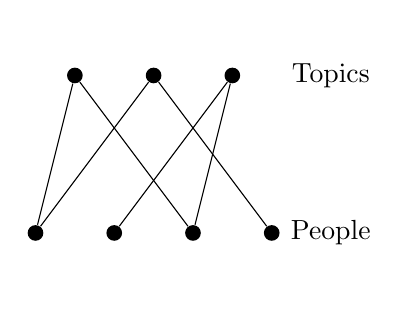
\begin{tikzpicture}[scale=1, every node/.style={circle, fill=black, inner sep=2pt}]

% Nodes: Topics (top row)
\node (t1) at (0.5,2) {};
\node (t2) at (1.5,2) {};
\node (t3) at (2.5,2) {};

% Nodes: People (bottom row)
\node (p1) at (0,0) {};
\node (p2) at (1,0) {};
\node (p3) at (2,0) {};
\node (p4) at (3,0) {};

% Edges
\draw (t1) -- (p1);
\draw (t1) -- (p3);
\draw (t2) -- (p1);
\draw (t2) -- (p4);
\draw (t3) -- (p2);
\draw (t3) -- (p3);

% Labels
\node[draw=none, fill=none] at (3.75,2) {Topics};
\node[draw=none, fill=none] at (3.75,0) {People};

\end{tikzpicture}
\caption{\label{fig:Relevance-Graph}Relevance Graph}
\end{figure}

Optionally, we can assign a weight $w_{ij} \in [0,1]$ to the edges of the graph to indicate the degree to which a person $j$ is affected by a topic $i$. A weight of $1$ could represent a life-or-death dependence, while a weight of $0$ would mean that the person is not affected at all. Figure \ref{fig:Relevance-Graph} shows an example of a relevance graph.

The relevance of a topic measures the extent to which it affects people. This can be assessed either by counting the number of affected individuals or by taking into account the magnitude of the effect.

\begin{definition}\index{Relevance}
\label{def:relevance}
Let $t \in \mathcal{T}$ be a topic, $\mathcal{P}_t \subseteq \mathcal{P}$ the set of people connected to $t$ in the relevance graph, and $w_{tp} \in [0,1]$ the weight of the edge between $t$ and $p \in \mathcal{P}_t$. We define the \emph{relevance} of $t$ as
\[
R(t) = \sum_{p : (t,p) \in E} w_{tp},
\]
\end{definition}

The unweighted relevance $R(t)$ (with $w_{tp} = 1$) counts the number of people affected by the topic, while the weighted relevance $R(t)$ reflects both the number of people and the severity of the effect. A higher relevance value indicates greater potential for generating important and impactful questions.

In practice it is useful to normalize the relevance of a topic so that the least relevant topic has a value of $0$, the most relevant has a value of $1$, and all others lie proportionally in between.

\begin{definition}\index{Normalized relevance}
\label{def:minmax_normalized_relevance}
Let $t \in \mathcal{T}$ be a topic. We define the \emph{min-max normalized relevance} of $t$ as
\[
\bar{R}(t) = \frac{R(t) - \min_{t' \in \mathcal{T}} R(t')}{\max_{t' \in \mathcal{T}} R(t') - \min_{t' \in \mathcal{T}} R(t')}
\]
\end{definition}

This transformation ensures that $\bar{R}(t) \in [0,1]$, with $0$ assigned to the least relevant topic and $1$ to the most relevant. In the degenerate case where all topics have the same relevance, all normalized values are set to $0$.

We could also compute the weighted degree of a person $p$, denoted $R(p)$, defined as the sum of the weights of the edges that link $p$ to topics in the relevance graph. This quantity measures the overall impact of all topics on a particular person. However, this measure is not used in the theory of nescience.

The relation between the weighted relevance of topics and the weighted degrees of people is given by the weighted degree sum formula:
\[
\sum_{t \in \mathcal{T}} R(t) \;=\; \sum_{p \in \mathcal{P}} R(p) \;=\; \sum_{(t,p) \in E} w_{tp}.
\]
In the unweighted case ($w_{tp} = 1$ for all edges), this formula reduces to the standard degree sum formula
\[
\sum_{t \in \mathcal{T}} \deg(t) \;=\; \sum_{p \in \mathcal{P}} \deg(p) \;=\; d(E).
\]

The next proposition shows that, in the weighted case, adding more topics to a research project can only increase its overall relevance. Of course, a research project dealing with "life, the universe, and everything" would be highly relevant, but also highly impractical. How to properly combine research topics will be described in Section \ref{sec:New_Research_Topics}.

\begin{proposition}
Let $S \subseteq \mathcal{T}$ be a finite set of topics and let $t' \in \mathcal{T} \setminus S$ be an additional topic. Then
\[
R(S \cup \{t'\}) \;\geq\; R(S),
\]
where the total weighted relevance of a set of topics $S$ is defined as
\[
R(S) = \sum_{\substack{t \in S \\ p \in \mathcal{P} \\ (t,p) \in E}} w_{tp}.
\]
\end{proposition}
\begin{proof}
We can write
\[
R(S \cup \{t'\}) = \sum_{\substack{t \in S \cup \{t'\} \\ p \in \mathcal{P} \\ (t,p) \in E}} w_{tp}
= R(S) + \sum_{\substack{p \in \mathcal{P} \\ (t',p) \in E}} w_{t'p}.
\]
Since all weights $w_{tp}$ are non-negative,
\[
\sum_{\substack{p \in \mathcal{P} \\ (t',p) \in E}} w_{t'p} \geq 0,
\]
which implies $R(S \cup \{t'\}) \geq R(S)$.
\end{proof}

This property shows that weighted relevance is monotone with respect to topic inclusion: if you enlarge the set of topics under consideration, the total weighted relevance can never decrease. In other words, adding topics can only maintain or increase the number (or severity) of connections to people in the relevance graph.

%
% Applicability
%

\section{Applicability}
\label{sec:applicability}

In this section, we introduce a new metric, applicability, which measures the potential of a research topic to serve as a tool for understanding or solving problems in other topics. The intuition is that some topics act as powerful enablers: mastering them allows progress to be made in many other areas.

From a formal standpoint, we say that a topic $t_j$ can be applied to a topic $t_i$ if the conditional nescience of $t_i$ given $t_j$ is smaller than the unconditional nescience of $t_i$ (see Section \ref{sec:conditional_nescience}).

Before defining applicability formally, we introduce the applicability graph, which encodes which topics have been successfully applied to others. This is a directed graph whose nodes are research topics, and where an arc from $t_j$ to $t_i$ indicates that $t_j$ has been successfully applied to explain or solve $t_i$.

\begin{definition}\index{Applicability graph}
\label{def:applicability-graph}
We define the \emph{applicability graph}, denoted by $AG$, as the directed graph $AG = (\mathcal{T}, E)$, where $\mathcal{T}$ is the set of research topics, and $E \subseteq \{ (i,j) : i,j \in \mathcal{T} \}$ is the set of arcs. An arc $(i,j)$ belongs to $E$ if $N(t_i \mid t_j) < N(t_i)$, that is, knowing $t_j$ reduces the nescience of $t_i$. The weight of the arc $(i,j)$ is defined as $w_{ij} = N(t_i) - N(t_i \mid t_j)$, representing the reduction in nescience obtained by applying $t_j$ to $t_i$.
\end{definition}

\begin{figure}[t]
\centering
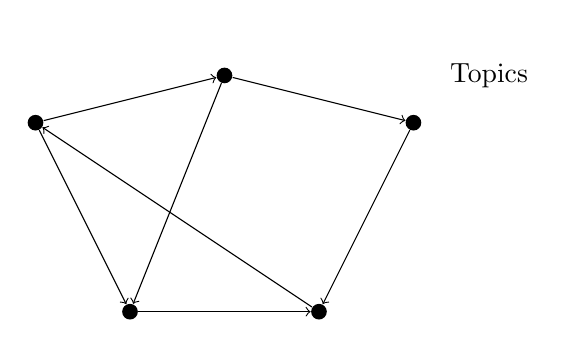
\begin{tikzpicture}[scale=1.2, every node/.style={circle, fill=black, inner sep=2pt}]

% Nodes (topics)
\node (t1) at (0,2) {};
\node (t2) at (2,2.5) {};
\node (t3) at (4,2) {};
\node (t4) at (1,0) {};
\node (t5) at (3,0) {};

% Directed edges
\draw[->] (t1) -- (t4);
\draw[->] (t1) -- (t2);
\draw[->] (t2) -- (t3);
\draw[->] (t2) -- (t4);
\draw[->] (t3) -- (t5);
\draw[->] (t4) -- (t5);
\draw[->] (t5) -- (t1);

% Labels
\node[draw=none, fill=none] at (4.8,2.5) {Topics};

\end{tikzpicture}
\caption{\label{fig:ApplicabilityGraph}Example of an applicability graph.}
\end{figure}

The applicability of a topic measures the total reduction in nescience it has produced when applied to other topics.

\begin{definition}\index{Applicability}
\label{def:applicability}
Given the applicability graph $AG = (\mathcal{T}, E)$, the \emph{applicability} of a topic $t_i \in \mathcal{T}$, denoted $A(t_i)$, is defined as
\[
A(t_i) = \sum_{(i,j) \in E} w_{ij},
\]
where the sum is over all arcs leaving $t_i$.
\end{definition}

A topic with high applicability is a versatile tool, capable of contributing to the understanding of many other topics. Intuitively, if a tool has been successfully applied multiple times in the past, it is more likely to be useful for solving new problems in the future.

As with relevance, applicability is monotone with respect to topic inclusion: combining topics can only increase their total applicability.

\begin{proposition}
\label{prop:nondecreasing_applicability}
Let $S \subseteq \mathcal{T}$ be a finite set of topics and $t' \in \mathcal{T} \setminus S$ an additional topic. Then
\[
A(S \cup \{t'\}) \geq A(S),
\]
where
\[
A(S) = \sum_{\substack{t \in S \\ (t,j) \in E}} w_{tj}.
\]
\end{proposition}
\begin{proof}
We can write
\[
A(S \cup \{t'\}) = A(S) + \sum_{(t',j) \in E} w_{t'j}.
\]
Since all weights $w_{ij}$ are non-negative,
\[
\sum_{(t',j) \in E} w_{t'j} \geq 0,
\]
which implies $A(S \cup \{t'\}) \geq A(S)$.
\end{proof}

This property ensures that adding more tools to a research effort can only maintain or increase its applicability.

To compare applicability values across topics on a standard scale, we define a normalized measure using min-max normalization.

\begin{definition}\index{Normalized applicability}
\label{def:normalized-applicability}
Given the applicability graph $AG = (\mathcal{T}, E)$, we define the \emph{min–max normalized applicability} of a topic $t_i \in \mathcal{T}$, denoted $\tilde{A}(t_i)$, as
\[
\tilde{A}(t_i) =
\frac{A(t_i) - \min_{t_k \in \mathcal{T}} A(t_k)}
     {\max_{t_k \in \mathcal{T}} A(t_k) - \min_{t_k \in \mathcal{T}} A(t_k)}
\]
where $A(t_i)$ is the applicability of $t_i$ as in Definition \ref{def:applicability}.
\end{definition}

This normalization ensures that $\tilde{A}(t_i) \in [0,1]$, with $0$ assigned to the least applicable topic and $1$ to the most applicable. In the degenerate case where all topics have the same applicability, all normalized values are set to 0. Note that min-max normalization can be sensitive to extreme values: if a single topic has exceptionally high applicability, the normalized scores of all other topics will be compressed toward zero.

In practice, computing the exact applicability graph is difficult because, for most topics, $N(t_i \mid t_j)$ is not known. We can approximate it by using a \emph{simplified applicability graph}, where arcs are unweighted and represent known instances of one topic being applied to another.

\begin{definition}\index{Simplified applicability graph}
\label{def:simplified-applicability-graph}
We define the \emph{simplified applicability graph}, denoted $SAG$, as the directed graph $SAG = (\mathcal{T}, E)$,
where $\mathcal{T}$ is the set of research topics, and $E \subseteq \{ (i,j) : i,j \in \mathcal{T} \}$ contains an arc $(i,j)$ if topic $j$ has been used to understand topic $i$.
\end{definition}

Using the simplified applicability graph, we can define an unweighted applicability measure.

\begin{definition}\index{Simplified applicability}
\label{def:simplified-applicability}
Given $SAG = (\mathcal{T}, E)$, the \emph{simplified applicability} of a topic $t \in \mathcal{T}$, denoted $SA(t)$, is the outdegree of $t$ in $SAG$, $SA(t) = \mathrm{outdeg}(t)$.
\end{definition}

Finally, we normalize simplified applicability to the range $[0,1]$:

\begin{definition}\index{Normalized simplified applicability}
\label{def:normalized-simplified-applicability}
Given the simplified applicability graph $SAG = (\mathcal{T}, E)$, we define the \emph{min–max normalized simplified applicability} of a topic $t_i \in \mathcal{T}$, denoted $SA_n(t_i)$, as
\[
SA_n(t_i) =
\frac{SA(t_i) - \min_{t_k \in \mathcal{T}} SA(t_k)}
     {\max_{t_k \in \mathcal{T}} SA(t_k) - \min_{t_k \in \mathcal{T}} SA(t_k)}
\]
where $SA(t_i)$ is the simplified applicability of $t_i$ as in Definition \ref{def:simplified-applicability}.
\end{definition}

This normalization ensures that $SA_n(t_i) \in [0,1]$, with $0$ assigned to the least applicable topic and $1$ to the most applicable. In the degenerate case where all topics have the same applicability, all normalized values are set to 0. As with the weighted case, min-max normalization may be sensitive to extreme values.

%
% Section: Maturity
%

\section{Maturity}
\label{sec:intro_maturity}

When selecting topics to use as tools, we are primarily interested in those that are well understood. Relying on background knowledge that is poorly understood is generally unwise, even if it appears to significantly reduce the conditional nescience of our main problem.

We therefore introduce the concept of the maturity of a topic, which measures the degree to which a topic is understood. Maturity is defined as the inverse of the nescience of the topic: the lower the nescience, the higher the maturity.

\begin{definition}\index{Maturity}
\label{def:maturity}
Let $t \in \mathcal{T}$ be a topic, and let $N(t)$ denote its nescience.
The \emph{maturity} of $t$, denoted $M(t)$, is defined as $M(t) = \frac{1}{N(t)}$.
\end{definition}

A higher maturity value indicates that the topic is better understood, and thus more suitable to be used as a tool in solving other problems. Conversely, highly immature topics (low $M(t)$) should be avoided as tools, since applying them would risk transferring our lack of understanding from one domain to another.

\begin{example}
Linear regression is a highly mature topic, since its nescience is very small, and so, its maturity is large.
\end{example}

To compare maturity values across topics on a standard scale, we define a min-max normalized version. This transformation assigns $0$ to the least mature topic, $1$ to the most mature, and scales all others proportionally.

\begin{definition}\index{Normalized maturity}
\label{def:normalized-maturity}
Given the set of topics $\mathcal{T}$, the \emph{min-max normalized maturity} of a topic $t \in \mathcal{T}$, denoted $\tilde{M}(t)$, is
\[
\tilde{M}(t) =
\frac{M(t) - \min_{t' \in \mathcal{T}} M(t')}
     {\max_{t' \in \mathcal{T}} M(t') - \min_{t' \in \mathcal{T}} M(t')}
\]
where $M(t)$ is the maturity of $t$ as in Definition \ref{def:maturity}.
\end{definition}

Min-max normalization ensures $\tilde{M}(t) \in [0,1]$, facilitating direct comparison between topics. However, as with other metrics, extreme outliers in maturity can compress the normalized values of the remaining topics toward zero.

%
% Section: Interestingness
%

\section{Interestingness}
\label{sec:interestingness-metrics}

We measure the interest of a topic in two complementary ways: as a tool, based on its usefulness in solving other problems; and as a problem, by studying its intrinsic research value.

The interestingness of a topic as a tool reflects how likely it is that the topic can be successfully applied to solve new problems. This likelihood depends on two key factors: maturity, or how well the topic is understood; and applicability, how widely it has been applied to other problems. We combine normalized measures of these two quantities into a single score:

\begin{definition}\index{Interestingness of a topic as a tool}
We define the \emph{interestingness as a tool} of $t$ as
\[
IT(t)=\frac{\sqrt{\,\tilde{M}(t)^2+\tilde{A}(t)^2\,}}{\sqrt{2}}
\]
\end{definition}

A topic will have a high $IT_n(t)$ value when it is both well understood ($\tilde{M}(t)$ close to $1$) and widely applicable ($\tilde{A}(t)$ close to $1$). In other words, the most interesting tools are those that combine deep understanding with broad utility in solving other problems.

\begin{example}
The Pythagorean theorem\index{Pythagorean theorem} (in a right-angled triangle, the square of the length of the hypotenuse is equal to the sum of the squares of the other two sides) is undoubtedly one of the most widely used and applied theorems in various fields and practical situations, including but not limited to: engineering (calculating distances, angles, and forces in structures and mechanical systems), architecture (determining lengths and angles in building design and construction projects), land surveying (measuring distances and calculating areas of land parcels), physics (analyzing problems in mechanics, optics, and electromagnetism), computer graphics and game development (calculating distances and angles in 2D and 3D spaces) or trigonometry(serving as a foundation for the study of trigonometric functions and their applications).
\end{example}

Some topics may have little utility as tools but are nonetheless highly valuable as research problems in their own right. To capture this idea, we define the interestingness of a topic as a problem, which reflects how compelling it is to investigate the topic itself. This depends on two main factors: relevance, or the degree to which the topic impacts people's lives; and nescience, as a measure of the extent to which the topic is not yet well understood.

\begin{definition}\index{Interestingness of a topic as a problem}
The \emph{interestingness as a problem} of $t$ is
\[
IP(t)=\frac{\sqrt{\,\tilde{N}(t)^2+\bar{R}(t)^2\,}}{\sqrt{2}}
\]
\end{definition}

Intuitively, a topic is interesting as a problem worth investigating if it has a large relevance (it has high impact in people's life) and a large nescience (it is not very well understood). In this sense, we are borrowing ideas from Popper's falsificationism: the more risky is a conjecture, the higher the advance achieved in science given its confirmation.

\begin{example}
World War I is a very relevant topic, because it had a huge impact on many people's life, and also it is not very well understood topic, since it takes hundreds of pages to explain its causes, and there is no general agreement among the specialists. So, according to our definition, it is a very interesting research problem.
\end{example}

%
% Section: Interesting Questions
%

\section{Interesting Questions}
\label{sec:interestingness-metrics}

In the theory of nescience we distinguish two kinds of unknowns, the known unknown and the unknown unknown. By known unknown we mean all those already known problems for which we do not know their solutions, for example, nobody knows how to cure diabetes, but we know what diabetes is and we are aware that nobody knows how to cure it. By unknown unknown we mean the collection of unknown problems, that is, all those problems that have not been found yet. In this section we focus on tools to takcle known unknown.

In our methodology, an interesting question emerges from the combination of two pre-existing topics. An interesting question is an ordered pair of topics $t$ and $p$, where $t$ has high interestingness as a tool, and $p$ has high interestingness as a problem.

\begin{definition}\index{Question}
Given $t, p\in\mathcal{T}$, we call \emph{question}\index{Question} the ordered pair $Q_{t\to p}=(t,p)$.
\end{definition}

Given a pair of a topics in $t_1, t_2 \in \mathcal{T}$, the question can be framed as "can we apply the tool described by topic $t_1$ to solve the problem described by topic $t_2$?".

The most interesting questions arise when topic $t_1$ exhibits high interestingness as a tool, and topic $t_2$ exhibits high interestingness as a problem. We define the interestingness of a question using the Euclidean distance, considering the interestingness of topics $t_1$ and $t_2$ as points in a two-dimensional space. The coordinates of these points are $(A_{t_1}, M_{t_1})$ for the tool and $(R_{t_2}, N_{t_2})$ for the problem. The distance between these points reflects how promising the combination of $t_1$ as a tool and $t_2$ as a problem is.

\begin{definition}\index{Interestingness of a question}
We define the interestingness of $Q_{t\to p}$ as
\[
IQ(t\to p)=\frac{\sqrt{\,IT(t)^2+IP(p)^2\,}}{\sqrt{2}}
\]
\end{definition}

Using the Euclidean distance in this way provides a clear geometric interpretation of a question's interestingness in the two-dimensional interestingness space. The greater the magnitude of the resulting vector, the more interesting the question is likely to be.

\begin{figure}[t]
\centering
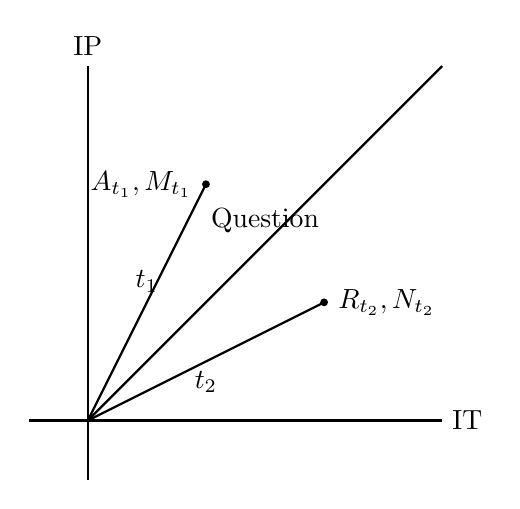
\begin{tikzpicture}[scale=1.5, axis/.style={thick}, vector/.style={thick},
                    point/.style={circle, inner sep=1pt, fill, color=black}
]

% Coordinate axes
\draw[axis] (-0.5, 0) -- (3, 0) node[right] {IT};
\draw[axis] (0, -0.5) -- (0, 3) node[above] {IP};

% Points for t1 and t2
\coordinate (t1) at (1, 2);
\coordinate (t2) at (2, 1);
\coordinate (iq) at (3, 3);

% Vectors for t1, t2, and the sum
\draw[vector] (0, 0) -- node[pos=0.5, above] {$t_1$} (t1);
\draw[vector] (0, 0) -- node[pos=0.5, below] {$t_2$} (t2);
\draw[vector] (0, 0) -- node[pos=0.5, above] {Question} (iq);

% Points and labels for t1 and t2
\node[point, label={left:$A_{t_1}, M_{t_1}$}] at (t1) {};
\node[point, label={right:$R_{t_2}, N_{t_2}$}] at (t2) {};

\end{tikzpicture}
\caption{\label{fig:InterestingQuestion}Example of an interesting quetion.}
\end{figure}

In practice, we must calculate all possible combinations of topics with high interestingness as tools and those with high interestingness as problems. We then select the combinations with the highest interestingness as questions. Naturally, most questions generated using this approach will be meaningless, much like those arising during brainstorming sessions when researchers attempt to identify new tools for tackling difficult problems.

This methodology can be applied in other scenarios as well. For instance, a researcher familiar with problem $p$ might be interested in finding applicable tools to solve it. Similarly, a researcher specializing in tool $t$ may be interested in discovering open problems where his expertise can be applied.

The above procedure can be easily generalized to encompass multiple tools and possibly multiple problems. This leads to the application of two tools to a given problem ($ t_1 + t_2 \rightarrow p$), the application of a single tool to the combination of two problems ($t \rightarrow p_1 + p_2$), and so on. The exact meaning of these tool and problem combinations depends on the topics themselves.

An interesting question is intradisciplinary if it combines two topics that are studied in the framework of the same research area (e.g., computer science). An interesting question is interdisciplinary if it combines two topics of different research areas (e.g., computer science and philosophy). In principle, the most innovative questions would be interdisciplinary questions, because the probability that somebody has thought about them is lower, since it requires specialists in both research areas working together to come up with that particular question.

\begin{definition}\index{Intradisciplinary question}\index{Interdisciplinary question}
Let $\mathcal{A}\subseteq\mathcal{T}$ be a research area. The question $Q_{t\to p}$ is \emph{intradisciplinary}\index{Intradisciplinary question} if $t,p\in\mathcal{A}$; otherwise it is \emph{interdisciplinary}\index{Interdisciplinary question}.
\end{definition}

\begin{example}
We could combine the topics with high interestingness as tools found in the area of "computer science" with those topics with high interestingness as problems found in the area of "biochemistry" in order to find new interesting interdisciplinary questions. Some examples of the kind of questions we can find with this approach include: "can we use regular expressions to identify DNA genes?" or "can we use a recursive algorithm to characterize proteins tertiary structure?"
\end{example}

The most innovative questions tend to be interdisciplinary, as they have a lower likelihood of having been considered previously. This is because they require collaboration between specialists from different research areas. 

%
% Section: New Research Topics
%
\section{New Topics}
\label{sec:new-topics}

The area composed by the unknown unknown problems is a highly interesting one, since it contains those research topics that will be addressed in the future. One of the main goals of this book is to help scientists discover the topics that lay in this unknown unknown area, since that would bring to the present the research problems of the future. In this section we focus on how to indentify the topics hidden in the unknown unknown area.

\begin{definition}\index{New topic}
Given $t_1,t_2\in T'$, a (candidate) \emph{new topic} from their combination is the unordered pair
\[
S_{\{t_1,t_2\}}=\{t_1,t_2\}.
\]
Associate $v(t)=(\tilde{N}(t),\bar{R}(t))$ and define the combination vector $v^\oplus(t_1,t_2)=v(t_1)+v(t_2)$.
\end{definition}

The exact meaning of the new topic that results as the combination of topics $t_{1}$ and $t_{2}$ is left to the creative interpretation of the researcher.

\begin{definition}\index{Interestingness of a new topic}
We define the interestingness of $S_{\{t_1,t_2\}}$ as
\[
IS(\{t_1,t_2\})=\frac{\sqrt{\,IT(t_1)^2+IT(t_2)^2\,}}{\sqrt{2}}
\]

\end{definition}

In practice, what we have to do is to compute all possible combination of those topics with very large interestingness as problems $IP_{t}$ with themselves, and select the combinations with higher $IS$. Of course, some of the combinations generated would be totally meaningless. Advanced techniques from the area of natural language processing or machine learning could be used to try filter out those nonsense combinations.

\begin{definition}\index{Intradisciplinary new topic}\index{Interdisciplinary new topic}
Let $\mathcal{A}\subseteq\mathcal{T}$. The new topic $S_{\{t_1,t_2\}}$ is \emph{intradisciplinary} if $t_1,t_2\in\mathcal{A}$; otherwise it is \emph{interdisciplinary}.
\end{definition}

Again, the most innovative new topics would be by the combination of interdisciplinary topics, because the probability that somebody has already though about them is lower.

%
% References
%

\section*{References}

The following works provide theoretical and philosophical foundations for the concepts of interestingness, maturity, and the combination of topics as tools and problems.

\cite{chalmers2013thing} An accessible introduction to the philosophy of science, addressing how scientific questions are formulated, evaluated, and justified.

\cite{pearl2019book} Introduces the principles of causal reasoning, crucial for determining whether applying one topic as a tool can effectively address another as a problem.

\cite{popper2014conjectures} Discusses falsifiability, novelty, and the importance of bold conjectures—foundational ideas for the “new and original” criterion.

\cite{shmueli2010explain} Clarifies the distinction between explanatory and predictive goals, helping to differentiate between topics valuable as problems versus tools.

\cite{van1980scientific} Explores the aims of science, model construction, and empirical adequacy, offering a philosophical context for defining “interesting” research.


%
%
% PART 2.- APPLICATIONS
%
%

\part{Part 2: Applications}
\label{part:Applications}

%
% CHAPTER: Machine Learning
%

%
% CHAPTER: Machine Learning
%

\chapterimage{Capek_play.pdf}

\chapter{Machine Learning}
\label{chap:Machine-Learning}

\begin{quote}
\begin{flushright}
\emph{There are no difficult problems,\\
only lack of imagination.}\\
Antonio García \\
\end{flushright}
\end{quote}
\bigskip

We have seen that the most difficult problems to which we can apply the results of the theory of nescience arise when set of entities $\mathcal{E}$ under study is composed by abstract elements. The difficulty with abstract entities is that it does not exits a way to encode them as strings of symbols so we can effectively reconstruct them. In practice, a possible approach to deal with this problem is to run an experiment and collect the results, as we do in case of physics. An alternative approach would be to take a collection of measurements, like for example, by means of observing the behavior of users in an online social network.

This chapter is devoted to how to apply the concept of minimum nescience to the area of machine learning. We assume that the entities under study are encoded as a dataset $\mathbb{X}$ composed by $n$ training vectors of $p$ predictors and a response variable $\bold{y}$ (see Section \ref{sec:machine_learning}).

We will start by providing practical approximations for the concepts of miscoding, inaccuracy and surfeit when the entities are encoded as datasets, and then we will show how to combine them in the single quantity of nescience. These approximations will allow us to introduce the \emph{minimum nescience principle}, a technique designed to automate the process of finding optimal models in machine learning (auto-machine learning). 

Besides introducing these approximations, we will show how to apply them to solve practical problems. The examples will be based on the \texttt{fastautoml} library, an open source python library that provides an implementation of the ideas included in this chapter.

%
% Section: Nescience Library
%

\section{Nescience Python Library}

The \texttt{fastautoml} library is an open source Python library that provides an implementation of the ideas included in this book applied to the area of machine learning. The library follows the API and conventions of the highly popular \texttt{scikit-learn} machine learning tool suite, and so, it can be combined with the methods provided by this package.

The \texttt{fastautoml} library can be installed with the \texttt{pip} utility:

\begin{sourcecode}
{\scriptsize \begin{verbatim}
pip install fastautoml
\end{verbatim}}
\end{sourcecode}

In the web page that accompanies this book, the reader can find a collection of notebooks for the \texttt{jupyter-lab} environment describing how the library works. For each subsection of this chapter, there is a notebook that implements all the examples included, so that the reader can repeat and play with them. Additional information about the \texttt{fastautoml} library, and a reference of the API provided, can be also found in the web page of the book.

%
% Section: Inaccuracy
%

\section{Inaccuracy}
\label{sec:machine_learning:inaccuracy}

In Section \ref{sec:inaccuracy:inaccuracy} we defined the inaccuracy of a description $d \in \mathcal{D}$ for a representation $r \in \mathcal{R}$ as the normalized information distance between the representation $r$ and the string $\Gamma(d)$ printed out by a universal Turing machine when given the description as input:
\[
\iota(d, r) = \frac{ \max\{ K \left(r \mid \Gamma(d) \right), K \left( \Gamma(d) \mid r \right) \} } { \max\{ K(r), K \left(\Gamma(d) \right) \} }
\]

Inaccuracy, being based in Kolmogorov complexity, is not computable for the general case, and so, it has to be approximated in practice. In this section we are going to see how this concept can be estimated in case of a model trained using a dataset. The approach will be similar to the one used in case of miscoding (see Section \ref{sec:approx-miscoding} for more information).

Given a training dataset $\mathbb{X}$ and a target variable $\mathbf{y}$, we can approximate the inaccuracy of a model $m$ as a predictor of $\mathbf{y}$ by means of computing the normalized compression distance between the predicted values $\mathbf{\hat{y}} = m(\mathbb{X})$ and the observed values $\mathbf{y}$. The Kolmogorov complexity $K(\mathbf{v})$ of a vector $\mathbf{v}$ will be approximated by the length of the compressed version of that vector $\hat{K}_C(\mathbf{v})$ using as compressor a minimal length code $C$, computed given the relative frequencies of the values observed in the vector $\mathbf{v}$ (see Section \ref{sec:approx-miscoding}).

{\color{red} TODO: This definition correspond to the discriminative case. Introduce the generative case as well.}

\begin{definition}
Let $\mathbb{X}$ be a dataset, $\mathbf{y}$ a response variable, $m$ a model, and $\mathbf{\hat{y}} = m(\mathbb{X})$ the predicted values by $m$ given $\mathbb{X}$. We define the \emph{inaccuracy}\index{Inaccuracy} of the model $m$ for the target values $\mathbf{y}$, denoted by $\hat\iota(\mathbf{\hat{y}}, \mathbf{y})$, as:
\[
\hat\iota(\mathbf{\hat{y}}, \mathbf{y}) = \frac{ \hat{K}_C(\mathbf{\hat{y}}, \mathbf{y}) - \min\{ \hat{K}_C(\mathbf{\hat{y}}), \hat{K}_C(\mathbf{y}) \} } { \max\{ \hat{K}_C(\mathbf{\hat{y}}), \hat{K}_C(\mathbf{y}) \} }
\]\end{definition}

Intuitively, the quantity $\hat\iota(\mathbf{\hat{y}}, \mathbf{y})$ is a measure of how far are the predicted values from real values. The lower this quantity, the better is the quality of $m$ as a predictor for $\mathbf{y}$. With our new inaccuracy metric we are measuring not only how difficult is to reconstruct the original target vector $\mathbf{y}$ given the predicted values $\mathbf{\hat{y}}$, but also how much additional information $\mathbf{\hat{y}}$ contains that is not related to $\mathbf{y}$, being the latter a novelty with respect to other metrics used in machine learning to measure the accuracy of a model.

\begin{example}
\label{ex:machine_learning:inaccuracy:inaccuracy_DT}
Inaccuracy, according to the minimum nescience principle, is given by the normalized compression distance between the actual targets $\mathbf{y}$ and the predicted targets $\mathbf{\hat{y}}$ by the model. In the following example we are going to compare the behavior of our new inaccuracy metric with a classical score metric. The experiment will be based on the MNIST\index{MNIST} dataset (hand written digits recognition) provided by scikit-learn.

\begin{sourcecode}
{\scriptsize \begin{verbatim}
from fastautoml.fastautoml import Inaccuracy
from sklearn.datasets import load_digits

X, y = load_digits(return_X_y=True)

inacc = Inaccuracy()
inacc.fit(X, y)
\end{verbatim}}
\end{sourcecode}

For this example we will train a decision tree classifier up to a pre-determined tree depth of $i$, where $i$ goes from $1$ to $20$.

\begin{sourcecode}
{\scriptsize \begin{verbatim}
from sklearn.tree import DecisionTreeClassifier

scores       = list()
inaccuracies = list()

for i in range(20):
    
    tree = DecisionTreeClassifier(max_depth=i, random_state=42)
    tree.fit(X, y)
    
    scores.append(1 - tree.score(X, y))
    inaccuracies.append(inacc.inaccuracy_model(tree))
\end{verbatim}}
\end{sourcecode}

We are interested to compare the behavior of score (actually we are comparing against one minus score) and inaccuracy metrics. As we can see in Figure \ref{figure:machine_learning:inaccuracy:inaccuracy_DT}, both metrics present a similar behavior, having inaccuracy a larger value, due to a stronger emphasis in incorrectly predicted values.

\begin{figure}[h]
\centering
\includegraphics[width=0.6\textwidth]{inaccuracy_DT.png}
\caption{Inaccuracy vs. Score of Decison Trees}
\label{figure:machine_learning:inaccuracy:inaccuracy_DT}
\end{figure}

\end{example}

In Example \ref{ex:machine_learning:inaccuracy:inaccuracy_DT} we have seen that the deeper the tree, the smaller is the training error. Of course, the higher the value of $i$, the higher the risk of overfitting\index{Overfitting} the data. However, in case of inaccuracy we are not interested in avoiding overfitting, since overfitting is controlled by the metric of surfeit (see Section \ref{sec:machine_learning:surfeit}).

We can see inaccuracy as the effort, measured as the length of a computer program, required to fix the predictions made by a model. In this sense, according to the minimum nescience principle, it is not the same a model that makes one hundred times the same error than a model that makes one hundred different errors, since it should be easier to fix the former than the later (see Example \ref{ex:machine_learning:inaccuracy:one_hundred_errors}).

\begin{example}
\label{ex:machine_learning:inaccuracy:one_hundred_errors}
In this example we are going to use again a decision tree classifier, but this time it will be trained with the hyperparameter minimum number of samples per leaf node set to 5 (a common approach used in practice to avoid decision trees to overfit).

\begin{sourcecode}
{\scriptsize \begin{verbatim}
tree = DecisionTreeClassifier(min_samples_leaf=5)
tree.fit(X, y)
\end{verbatim}}
\end{sourcecode}

The inaccuracy of this new trained model is $0.17$, and its score $0.08$. Next we will artificially introduce one hundred errors in the dataset, simulating the case that the tree is not able to model correctly these data points. In this particular case all the errors are exactly the same.

\begin{sourcecode}
{\scriptsize \begin{verbatim}
X2 = X.copy()
y2 = y.copy()
for i in range(100):
    X2 = np.append(X2, [X[0]], axis=0)
    y2 = np.append(y2, (y[0]+1) % 10)
\end{verbatim}}
\end{sourcecode}

The inaccuracy of the decision tree, given this new dataset, has increased\footnote{Note that we had to \texttt{fit()} again the class Inaccuracy in order to use the new dataset. Normally this is not the way we use this class; instead what we should do is to fit once a dataset, and then compute the inaccuracy of different models. We are doing here in this way to demonstrate an interesting property of the concept of inaccuracy.} from $0.17$ to $0.21$.

\begin{sourcecode}
{\scriptsize \begin{verbatim}
inacc.fit(X2, y2)
inacc.inaccuracy_predictions(pred)
\end{verbatim}}
\end{sourcecode}

Score has also increased, in this case from $0.08$ to $0.13$.

\begin{sourcecode}
{\scriptsize \begin{verbatim}
1 - tree.score(X2, y2)
\end{verbatim}}
\end{sourcecode}

Finally, we are going to repeat exactly the same experiment, but this time instead of adding one hundred times the same error, adding one hundred different errors.

\begin{sourcecode}
{\scriptsize \begin{verbatim}
X3 = X.copy()
y3 = y.copy()
for i in arange(100):
    index = np.random.randint(X.shape[0])
    X3    = np.append(X3, [X[index]], axis=0)
    y3    = np.append(y3, (y[index]+1) % 10)
\end{verbatim}}
\end{sourcecode}

In this last case the inaccuracy of the model has increased up to $0.25$, meanwhile score remained the same.
\end{example}

In line with Example \ref{ex:machine_learning:inaccuracy:one_hundred_errors}, an extreme case would be a model for a target binary variable (True and False) that always fails with its predictions, that is, if the value of the target is True, the model will predict False, and if it is False, it will predict True. The classical evaluation metrics would say that this model is the worst possible model, but our inaccuracy would claim that the model is perfect. We might be wondering what it is the value of a model that always fails to predict the correct target. But if we are the managers of an edge fund investing in the stock market\index{Stock market}, we will very happy to pay a huge amount of money for a model that predicts that the shares of IBM will go down whenever they go up, and the other way around.

In case of having a highly unbalanced dataset\index{Unbalance dataset}, that is, when some categories have a lot of more training data than others, the classical score metric can provide a misleading result, since a good score does not necessarily mean a good model, it might happen that the model is simply properly classifying the samples of the category with the higher number of training samples, and misclassifying the others. In practice, we solve this problem by using metrics specifically designed to deal with unbalanced datasets. In case of the new metric of inaccuracy, as Example \ref{ex:machine_learning:inaccuracy:unbalanced_dataset} shows, a model that can not properly classify one of the categories is considered a bad model, even if this category has only a few points in the training dataset.

\begin{example}
\label{ex:machine_learning:inaccuracy:unbalanced_dataset}
For this example, we will create a synthetic dataset using the \texttt{make\_classification} utility of scikit-learn, with two classes in which one of then has 95\% of the samples, and the other 5\%.

\begin{sourcecode}
{\scriptsize \begin{verbatim}
from sklearn.datasets import make_classification

depth = list()
score = list()
inacc = list()

inaccuracy = Inaccuracy()

for i in np.arange(1, 100):
                    
    X, y = make_classification(n_samples=1000, n_features=2,
                               n_informative=2, n_redundant=0,
                               class_sep=2, flip_y=0, weights=[0.95,0.05])

    inaccuracy.fit(X, y)
        
    tree = DecisionTreeClassifier(min_samples_leaf=i)
    tree.fit(X, y)

    depth.append(i)        
    score.append(1 - tree.score(X, y))
    inacc.append(inaccuracy.inaccuracy_model(tree))
\end{verbatim}}
\end{sourcecode}

The experiment consists in training a decision tree classifier with a minimum number of samples per leaf of $i$, where $i$ goes from 1 to 100. In Figure \ref{figure:machine_learning:inaccuracy:inaccuracy_DT2} we can see the behavior of inaccuracy and score. In case of large values of $i$, the score metric tell us that no more than a 5\% of the samples is misclassified, however, the inaccuracy says that even if the total number of misclassified points is low, the inaccuracy of the model is very bad.

\begin{figure}[h]
\centering
\includegraphics[width=0.6\textwidth]{inaccuracy_DT2.png}
\caption{Inaccuracy of Decision Tree.}
\label{figure:machine_learning:inaccuracy:inaccuracy_DT2}
\end{figure}

\end{example}


%
% Section: Miscoding
%

\section{Miscoding}
\label{sec:approx-miscoding}

In Section \ref{def:miscoding} we introduced the concept of miscoding as a quantitative measure of how well a string based encoding $r \in \mathcal{R}$ represents a research entity from $\mathcal{E}$. The miscoding of a representation $r$ was defined as:
\[
\mu(r) = \overset{o}{ \underset{s \in \mathcal{R}_\mathcal{E}} \min} \frac{ \max\{ K(s \mid r), K(r \mid s) \} } { \max\{ K(s), K(r) \} }
\]
and we saw that this quantity cannot be computed in practice for the general case. First of all because it requires a computation from an abstract oracle machine, second because it is based on the uncomputable Kolmogorov complexity, and third because it does not take into account the entity $e$ in which we are interested. 

In this section we are going to see how this concept can be adapted in practice to compute the error made by using a dataset $\mathbb{X}$ as a representation of a response variable $\mathbf{y}$ (see Section \ref{sec:machine_learning}). Our goal is double, in one hand we are interested to measure the quality of the dataset $\mathbb{X}$ as a predictor of the variable $\mathbf{y}$, and in the other we want to identify those features $\mathbf{x}_j$ of $\mathbb{X}$ that have the higher predictive power for $\mathbf{y}$. In this context, the target variable $\mathbf{y}$ would play the role of the entity, and the dataset $\mathbb{X}$ the role of representation, so to speak.

Given a training dataset $\mathbb{X}$ composed by $n$ vectors with $p$ features, we can approximate the miscoding of a feature $\mathbf{x}_j$ for the target variable $\mathbf{y}$ by computing the normalized information distance between $\mathbf{x}_j$ and $\mathbf{y}$ (see Section \ref{sec:information_distance}):
\[
E(\mathbf{x}_j, \mathbf{y}) = \frac{\max\{ K(\mathbf{x}_j \mid \mathbf{y}), K(\mathbf{y} \mid \mathbf{x}_j) \}}{\max \{ K(\mathbf{x}_j), K(\mathbf{y}) \} }
\]
As it is customary, the Kolmogorov complexity $K(s)$ of a string $s$ will be approximated by the length of the compressed version of that string using a standard compressor, that is, we will use the normalized compression distance:
\[
E_Z(\mathbf{x}_j, \mathbf{y}) = \frac{\max\{ \hat{K}_Z(\mathbf{x}_j \mid \mathbf{y}), \hat{K}_Z(\mathbf{y} \mid \mathbf{x}_j) \}}{\max \{ \hat{K}_Z(\mathbf{x}_j), \hat{K}_Z(\mathbf{y}) \} }
\]
where $\hat{K}_Z(s)$ denotes the length of the compressed version of the string $s$ using the compressor $Z$. In the particular case of having a vector $\mathbf{x} = \{ x_1, \ldots, x_n \}$ of measurements, the string $s$ to be compressed will be the concatenation of the encoded values $s = \langle x_1, \ldots, x_n \rangle$. We prefer the following equivalent definition of normalized compression dinstance, since in practice it is easier to compute the joint distribution of two vectors than the conditional distribution:
\[
E_Z(\mathbf{x}_j, \mathbf{y}) = \frac{ \hat{K}_Z(\mathbf{x}_j, \mathbf{y}) - \min\{ \hat{K}_Z(\mathbf{x}_j), \hat{K}_Z(\mathbf{y}) \} } { \max\{ \hat{K}_Z(\mathbf{x}_j), \hat{K}_Z(\mathbf{y}) \} }
\]
As compression technique we will use a code $C$ with minimal length, given the relative frequencies of the different observed values (see Section \ref{sec:Optimal-Codes}). If $\mathbf{x}$ is a qualitative vector (either a feature or the target variable) taking values from a set labels $\mathcal{G} = \{g_1, \ldots, g_\ell\}$, that is $\mathbf{x} \in \mathcal{G}^n$, the quantity $\hat{K}_C(\mathbf{x})$ can be computed as:
\[
\hat{K}_C(\mathbf{x}) = - \sum_{i=1}^l \log_2{ \frac{ \sum_{j=1}^n I(x_j = g_i)} {n} } 
\]
If the case of $\mathbf{x}$ being based on a continuous random variable, we cannot calculate the probability of $x_j$ since, in general, the underline probability distribution of $\mathbf{x}$ is unknown. Moreover, we have that $P(x_j)=0$ for all $j$. In order to approximate the value $K(\mathbf{x})$ using a minimal length code $C$, we have to discretize first the vector $\mathbf{x}$ into a collection of intervals.

Given a continuous feature $\bold{x}_j$ composed by $n$ samples $\{x_{1j}, \ldots, x_{nj}\}$, a discretization algorithm will produce a finite non-overlapping partition of $m$ discrete intervals $D=\{ [d_o, d_1], (d_1, d_2], \ldots, (d_{m-1}, d_m] \}$, where $d_o = \min{\bold{x}_j}$, and $d_m = \max{\bold{x}_j}$, and $d_i < d_{i+1}$ for $i = 0, 1, \ldots, m-1$, and then it assigns a categorical value to each interval. We will use discretization to estimate the probability of a particular observation.

A discretization algorithm is a mapping between a (possibly huge) number of numeric values and a reduced set of discrete values, and so, it is a process in which some information is potentially lost. The choice of discretization algorithm is something that could have a high impact in the practical computation of the nescience. We are interested in a discretization algorithm that produces a large number of intervals (low bias), with a large number of number of observations per interval (low variance). Common techniques include \emph{equal width discretization}, \emph{equal frequency discretization} and \emph{fixed frequency discretization}. However, these techniques require the optimization of an hyperparameter, and so, they are not suitable for our purposes.

In the \texttt{fastautoml} library we use a \emph{proportional discretization approach}, where the number of intervals $m$ and the number of observations per interval $s$ are equally proportional to the number of observations $n$. The algorithm starts by sorting the values of $\bold{x}_j$ in ascending order and then discretizing them into $m$ intervals of approximately $s$ (possibly identical) values each. In this way, as the number of training observations increases, both interval frequency and number of intervals increases, taking advantage of the larger number of observations. In the same way, when the number of observations decreases, we reduce both. In particular, in the nescience library we set $s = m = \sqrt{n}$

The same procedure can be applied in case of having a discrete feature with too many labels compared with the number of samples.

Using this discretization procedure, we can approximate the Kolmogorov complexity of a vector $\mathbf{x}$ by:
\[
\hat{K}_C(\mathbf{x}) = - \sum_{i=1}^m \log_2{ \frac{ \sum_{j=1}^n I(x_j \in D_i)} {n} } 
\]
where $D_i$ is the interval defined by the end points $(i-1, i)$.

The quantity $\hat{K}_C$ can be generalized to the an arbitrary number of $m$ vectors $\hat{K}_C(\mathbf{x_1}, \ldots, \mathbf{x_m})$ composed by $n$ samples each, by considering the joint encoded vector
\[
\langle \mathbf{x_1}, \mathbf{x_2}, \ldots, \mathbf{x_m} \rangle = \{ \langle x_{11}, x_{12}, \ldots, x_{1m} \rangle, \ldots, \langle x_{n1}, x_{n2}, \ldots, x_{nm} \rangle \}
\]

Given the above considerations, we can provide the following approximation for the concept of miscoding for representations based on datasets.

\begin{definition}
Let $\mathbf{y}$ be a response variable, $\mathbb{X}$ a dataset composed by $p$ features, and $\mathbf{x}_j$ the $j-th$ feature. We define the feature miscoding of $\mathbf{x}_j$ as a representation of $\mathbf{y}$, denoted by $\hat\mu(\mathbf{x}_j, \mathbf{y})$, as:
\[
\hat\mu(\mathbf{x}_j, \mathbf{y}) = \frac{ \hat{K}_C(\mathbf{x}_j, \mathbf{y}) - \min\{ \hat{K}_C(\mathbf{x}_j), \hat{K}_C(\mathbf{y}) \} } { \max\{ \hat{K}_C(\mathbf{x}_j), \hat{K}_C(\mathbf{y}) \} }
\]\end{definition}

Intuitively, the quantity $\hat\mu(\mathbf{x}_j, \mathbf{y})$ is a measure of the effort, in relative terms, required to fully encode $\mathbf{y}$ assuming a knowledge of $\mathbf{x}_j$, and the other way around. The lower this value, the better is the quality of $\mathbf{x}_j$ as a predictor for $\mathbf{y}$.

\begin{example}

Let's $\mathbf{y}$ be a target variable composed by $1.000$ random samples that follows a normal distribution $N(3,1)$ with mean $\mu = 3$ and standard deviation $\sigma = 1$, $\mathbf{x}_1$ be a predictor feature that is equal to $\mathbf{y}$ with some random noise, that is $\mathbf{x}_1 = \mathbf{y} + N(0, 1)$, and $\mathbf{x}_2$ be a second predictor based on random samples from a exponential distribution with a rate of $\lambda = 1$.

\begin{sourcecode}
{\scriptsize \begin{verbatim}
from scipy.stats import norm, expon

y  = norm.rvs(loc=3, size=1000)
x1 = y + np.random.randn()
x2 = expon.rvs(size=1000)
\end{verbatim}}
\end{sourcecode}

We can use the Nescience library to compute the miscoding of the features $\mathbf{x}_1$ and $\mathbf{x}_2$ when they encode the target variable $\mathbf{y}$.

\begin{sourcecode}
{\scriptsize \begin{verbatim}
from Nescience.Nescience import Miscoding
import numpy as np

X = np.column_stack((x1, x2))

miscoding = Miscoding()
miscoding.fit(X, y)
miscoding.miscoding_features(type='regular')
\end{verbatim}}
\end{sourcecode}

The output of the library would be something similar to the following\footnote{Since we are generating a list of $1.000$ random samples, the reader could get a slightly different result when running this example.}:

\begin{sourcecode}
{\scriptsize \begin{verbatim}
array([0.        , 0.84443761])
\end{verbatim}}
\end{sourcecode}

As it was expected the miscoding of $\hat\mu(\mathbf{x}_1, \mathbf{y})$ is almost zero, meanwhile the miscoding of $\hat\mu(\mathbf{x}_2, \mathbf{y})$ is much higher. In this case, we should prefer $\mathbf{x}_1$ over $\mathbf{x}_2$ as a predictor of $\mathbf{y}$.

\end{example}

Sometimes we will use the normalized version of the complements of the individual miscodings, that is $\frac{ 1 - \hat\mu(\mathbf{x}_i, \mathbf{y}) } { \sum_{i=j}^p 1 - \hat\mu(\mathbf{x}_j, \mathbf{y}) }$, instead of the regular ones $\hat\mu(\mathbf{x}_i, \mathbf{y})$, because they are easier to compare with other feature selection techniques, and because they have a visually appealing interpretation. We call this version of miscoding the adjusted feature miscoding.

\begin{example}
In this example we are going to generate a synthetic dataset where the target variable $\mathbf{y}$ is a collection of normally-distributed clusters of points, and the training set $\mathbb{X}$ is composed by both, relevant and irrelevant predictors. In particular we will generate $1.000$ samples composed by $10$ features that describe $10$ clusters; only $4$ of the features are relevant for prediction, and the other remaining $6$ are just random values.

\begin{sourcecode}
{\scriptsize \begin{verbatim}
from Nescience.Nescience import Miscoding
from sklearn.datasets.samples_generator import make_classification

X, y = make_classification(n_samples=1000, n_features=10, n_informative=4,
       n_redundant=0, n_classes=10, n_clusters_per_class=1, flip_y=0)

miscoding = Miscoding()
miscoding.fit(X, y)
msd = miscoding.miscoding_features(miscoding='adjusted')
\end{verbatim}}
\end{sourcecode}

We will use the adjusted version of the miscoding for an easier comparison with other feature selection techniques. If we plot the results (see Figure \ref{figure:miscoding_make_classification}) we will see that the library has successfully identified the four relevant predictors ($\mathbf{x}_3$, $\mathbf{x}_8$, $\mathbf{x}_{10}$ and $\mathbf{x}_{16}$). Since we are using the adjusted version of miscodings, the actual values have to be interpreted in relative terms. 

\begin{figure}[h]
\centering
\includegraphics[width=0.6\textwidth]{feature_miscoding.png}
\caption{Miscoding of a Synthetic Dataset.}
\label{figure:miscoding_make_classification}
\end{figure}

We can compare miscoding with correlation, a common technique used in machine learning to identify the most relevant features of a dataset. In Figure \ref{figure:correlation_make_classification} is shown correlation between the individual features that compose $\mathbb{X}$ and the target variable $\mathbf{y}$. As we can observe, correlation fails to properly identify one of the relevant features ($\mathbf{x}_3$).

\begin{sourcecode}
{\scriptsize \begin{verbatim}
np.corrcoef(X, y)
\end{verbatim}}
\end{sourcecode}

\begin{figure}[h]
\centering
\includegraphics[width=0.6\textwidth]{feature_correlation.png}
\caption{Correlation of a Synthetic Dataset.}
\label{figure:correlation_make_classification}
\end{figure}

\end{example}

Feature miscoding allow us to identify the most relevant features of a training dataset $\mathbb{X}$, but it cannot be used to compute the miscoding of the dataset itself. If we start with a miscoding of $1$ (full unknown), and subtract the miscodings of the individual features, we will end up with a negative miscoding, something that it is not allowed by our theory. If we use the adjusted version, the dataset miscoding will be $0$ for all datasets, which is against our intuition that not all possible datasets $\mathbb{X}$ represent equally well a target variable $\mathbf{y}$. According to the theory of nescience, we expect that non-relevant features add, instead of subtract, to the global miscoding of the dataset.

In order to address this problem, we have to introduce the concept of partial miscoding of a feature, as the difference between the adjusted and normalized miscodings.

\begin{definition}
Let $\mathbf{y}$ be a target variable, $\mathbb{X}$ a dataset composed by $p$ features, and $\mathbf{x}_j$ the $j-th$ feature. We define the partial miscoding of $\mathbf{x}_j$ as a representation of $\mathbf{y}$, denoted by $\tilde\mu(\mathbf{x}_j, \mathbf{y})$, as:
\[
\tilde\mu(\mathbf{x}_i, \mathbf{y}) = \frac{ 1 - \hat\mu(\mathbf{x}_i, \mathbf{y}) } { \sum_{j=1}^p 1 - \hat\mu(\mathbf{x}_j, \mathbf{y}) } - \frac{\hat\mu(\mathbf{x}_i, \mathbf{y}) } { \sum_{j=1}^p \hat\mu(\mathbf{x}_j, \mathbf{y}) }
\]
\end{definition}

A positive partial miscoding means that the feature contributes to describe the target variable, meanwhile a negative value means that the feature is not relevant.

\begin{example}
\label{example:partial_feature_miscoding}
In this example we will use again a synthetic dataset composed by a collection of normally-distributed clusters of points, but we will increase the number of features to $20$, from which $14$ are relevant. Then, we will compute the list of partial miscodings.

\begin{sourcecode}
{\scriptsize \begin{verbatim}
from Nescience.Nescience import Miscoding
from sklearn.datasets.samples_generator import make_classification

X, y = make_classification(n_samples=1000, n_features=20, n_informative=14,
       n_redundant=0, n_classes=10, n_clusters_per_class=1, flip_y=0)

miscoding = Miscoding()
miscoding.fit(X, y)
msd = miscoding.miscoding_features(miscoding="partial")
\end{verbatim}}
\end{sourcecode}

As we can see in Figure \ref{figure:partial_feature_miscoding}, not only the library has been able to correctly identify the relevant features, but also, non relevant features have now a negative contribution to the global miscoding.

\begin{figure}[h]
\centering
\includegraphics[width=0.6\textwidth]{partial_miscoding.png}
\caption{Partial Feature Miscoding.}
\label{figure:partial_feature_miscoding}
\end{figure}

\end{example}

Given the definition of partial feature miscoding we can provide a definition of the concept of miscoding of a target variable given a subset of predictors that it is closer to the original concept of miscoding defined by the theory of nescience.

\begin{definition}
Let $\mathbf{y}$ be a target variable, $\mathbb{X} = \{ \mathbf{x}_1, \ldots, \mathbf{x}_p \}$ a dataset composed by $p$ features, and $\mathbb{Z} = \{ \mathbf{z}_1, \ldots, \mathbf{z}_k \}$ a subset of features, that is, $\{ \mathbf{z}_1, \ldots, \mathbf{z}_k \} \subseteq \{ \mathbf{x}_1, \ldots, \mathbf{x}_p \}$. We define the miscoding of $\mathbb{Z}$ as a representation of $\mathbf{y}$, denoted by $\hat\mu(\mathbb{Z}, \mathbf{y})$, as:
\[
\hat\mu(\mathbb{Z}, \mathbf{y}) = \sum_{i=1}^k \tilde\mu (\mathbf{z}_i, \mathbf{y})
\]
\end{definition}

A sensible approach to use the concept of partial miscoding in machine learning would be to incrementally add to our model those features with higher partial miscoding, until all features with a positive partial miscoding have been added, or a optimality criterion has been reached (see Example \ref{example:accumulated_partial_feature_miscoding}).

{\color{red} TODO: Prove that this approach is (near) optimal compared to evaluating all the possible feature combinations.}

\begin{example}
\label{example:accumulated_partial_feature_miscoding}
Based on the dataset and the partial features miscoding computed in Example \ref{example:partial_feature_miscoding}, in Figure \ref{figure:accumulated_partial_feature_miscoding} we can see the evolution of the miscoding of the training subset $\mathbb{Z}$ as we add more features to the study.

\begin{figure}[h]
\centering
\includegraphics[width=0.6\textwidth]{accumulated_partial_miscoding.png}
\caption{Accumulated Partial Feature Miscoding.}
\label{figure:accumulated_partial_feature_miscoding}
\end{figure}

\end{example}

In the following final example we are going to compare the performance of a machine learning classifier when using a full dataset and a reduced version of the same dataset using only those features identified as relevant, i.e., with positive partial miscoding.

\begin{example}
In this example we will train a neural network with the standard MNIST dataset in order to classify hand written digits. The evaluation criteria will be the score of the classifier, that is, the percentage of digits correctly classified, applied over a test dataset different from the dataset used for training. The neural network will be trained and evaluated using all the features that compose the dataset, and with a reduced version of the dataset composed by only those features with a positive partial miscoding.

\begin{sourcecode}
{\scriptsize \begin{verbatim}
import numpy  as np
from sklearn.model_selection import train_test_split
from sklearn.neural_network import MLPClassifier
from sklearn.datasets import load_digits
from Nescience.Nescience import Miscoding

data = load_digits()
X_raw = data.data
y_raw = data.target

miscoding = Miscoding()
miscoding.fit(X_raw, y_raw)
mscd = miscoding.miscoding_features(miscoding='partial')
X_red = X_raw[:,np.where(mscd > 0)[0]]
y_red = y_raw

X_raw_train, X_raw_test, y_raw_train, y_raw_test = train_test_split(X_raw,
             y_raw, test_size=.3)
X_red_train, X_red_test, y_red_train, y_red_test = train_test_split(X_red,
             y_red, test_size=.3)

clf = MLPClassifier(alpha=1, max_iter=1000)

clf.fit(X_raw_train, y_raw_train)
score_raw = clf.score(X_raw_test, y_raw_test)
        
clf.fit(X_red_train, y_red_train)
score_red = clf.score(X_red_test, y_red_test)
        
reduction = 1 - X_red_train.shape[1] / X_raw_train.shape[1]

print("Score raw:", score_raw, " Score Miscoding:", score_red,
      " Reduction:", reduction)
\end{verbatim}}
\end{sourcecode}

If we run the above source code, we will see that the score of the neural network classifier is about the same for the two datasets, 98\% of the digits are correctly classified using the test data. However, the reduced dataset used for training based on the optimal miscoding is 43\% smaller than the original dataset. This size reduction could have a big impact in the training time of the neural network. Smaller datasets are also relevant when working with ensembles of models, like random forests, where hundreds or thousands of models have to be trained.

\end{example}

Intuitively, as Example \ref{example:accumulated_partial_feature_miscoding} shows, we should prefer the subset $\mathbb{Z}$ of $\mathbb{X}$ composed by all those features whose partial miscoding are greater than zero. However, as we will see in the following sections of this chapter, this might not be the case. Feature selection is only one of the criteria used in the process of finding an optimal model for an entity represented by a dataset. It might happen that other elements, like inaccuracy or surfeit, suggest to use a different subset of predictors. The global optimization criteria we should use is the concept of nescience.


%
% Section: Surfeit
%

\section{Surfeit}
\label{sec:machine_learning:surfeit}

In Section \ref{sec:Definition_redundancy} we defined the surfeit of the model $m \in \mathcal{M}$ for the representation $r \in \mathcal{R}$ as:
\[
\sigma (m, r) = 1 - \frac{K(r)}{l(m)}
\]
Since the length $K(r)$ of shortest possible model for the representation $r$ is in general unknown, we have to approximate this concept in practice. In case of having a training dataset $\mathbb{X}$ and a target variable $\mathbf{y}$, we can approximate the surfeit of a model $m$ for the representation $\mathbf{y}$ by means of computing:
\[
\hat\sigma(m, y) = 1 - \frac{\hat{K}_C(\mathbf{y})}{l(m)}
\]
Where $\hat{K}_C(\mathbf{y})$ is the length of the compressed version of the of the vector $\mathbf{y}$ using as compressor a minimal length code $C$, computed given the relative frequencies of the values observed in $\mathbf{y}$ (see Section \ref{sec:approx-miscoding}).

\begin{definition}
Let $\mathbf{y}$ be a response variable, $\mathbb{X}$ a dataset composed by $p$ features and $n$ samples. We define the surfeit of the model $m \in \mathcal{M}$ as a representation of $\mathbf{y}$, denoted by $\hat\sigma(m, \mathbf{y})$, as:
\[
\hat\sigma(m, \mathbf{y}) = 1 - \frac{\hat{K}_C(\mathbf{y})}{l(m)}
\]
\end{definition}

The definition of surfeit requires a method of encoding the models as a string of symbols, so we can compute their length. Ideally, we should use as encodings Turing machines, and agree upon an universal Turing machine to interpret those models. However, that would make very difficult to add new models to the nescience library. Instead, we have used for the encoding of models a simplified version of the Python language, where not all the constructions are allowed, and we do not allow the use of libraries.

Surfeit is a metric that can help us to avoid overfitted models. The higher is the surfeit of a model, the higher is the probability that the model is an overfit of the training dataset, as Example \ref{ex:surfeit_overfit} shows.

\begin{example}
\label{ex:surfeit_overfit}
In this example we are going to generate a dataset composed by $900$ samples of a sinusoidal curve, and we will fit the data using a $n$ degree polynomial, where $n$ goes form $1$ to $15$.

\begin{sourcecode}
{\scriptsize \begin{verbatim}
from sklearn.linear_model import LinearRegression
from sklearn.preprocessing import PolynomialFeatures

from Nescience.Nescience import Surfeit
from Nescience.Nescience import Inaccuracy

n_samples = 900
degrees = np.arange(1, 15)

X = np.sort(np.random.rand(n_samples) * 3)
y = np.cos(1.5 * np.pi * X)

linacc   = list()
lsurfeit = list()

for i in degrees:
        
    poly = PolynomialFeatures(degree=i, include_bias=False)
    newX = poly.fit_transform(X[:, np.newaxis])
    
    linear_regression = LinearRegression()
    linear_regression.fit(newX, y)

    inacc.fit(newX, y)
    inaccuracy = inacc.inaccuracy_model(linear_regression)
    
    sft.fit(newX, y)
    surfeit = sft.surfeit_model(linear_regression)
    
    linacc.append(inaccuracy)
    lsurfeit.append(surfeit)
\end{verbatim}}
\end{sourcecode}

In figure \ref{figure:surfeit_vs_inaccuracy} we can see the results of this experiment. As it was expected, the higher the degree of the polynomial, the smaller is the error of the model. However, at the same time we see that the higher the polynomial, the higher the surfeit of the model. The ideal model is that one that has a low inaccuracy and a low surfeit.

\begin{figure}[h]
\centering
\includegraphics[width=0.6\textwidth]{surfeit_vs_inaccuracy.png}
\caption{Surfeit vs Inaccuracy}
\label{figure:surfeit_vs_inaccuracy}
\end{figure}

\end{example}

Another advantage of the concept of surfeit is that it allows us to compare and decide between models that belong to different families. For example, in case of models having the same accuracy, shall we prefer a decision tree over a neural network, or a naive Bayes classifier over a support vector machine? Next example shows how we can decide about those questions.

\begin{example}
\label{ex:dt_vs_nn}

In this example we are going to compare a decision tree with a neural network. We will use a synthetic dataset composed by two isotropic Gaussian blobs, and we will train our models to split them apart. In the first part of the example we will use a standard deviation of $1$ and only two dimensions, so the two clusters are easy to classify (see figure on Table \ref{tab:isotropic_gaussian_blobs}, left side).

\begin{table}
\begin{center}

\begin{tabular}{ c c }

\includegraphics[scale=0.4]{blobs_easy_split} & \includegraphics[scale=0.4]{blobs_difficult_split}

\end{tabular}
\end{center}
\caption{\label{tab:isotropic_gaussian_blobs}Isotropic Gaussian blobs.}
\end{table}

% \raisebox{.4\height}{\includegraphics[scale=0.4]{blobs_difficult_split}}

\begin{sourcecode}
{\scriptsize \begin{verbatim}
from sklearn.tree import DecisionTreeClassifier
from sklearn.neural_network import MLPClassifier
from Nescience.Nescience import Surfeit
from Nescience.Nescience import Inaccuracy
from sklearn.datasets.samples_generator import make_blobs

X, y = make_blobs(n_samples=1000, centers=2, n_features=2, cluster_std=1)

tree = DecisionTreeClassifier()
tree.fit(X, y)
tree.score(X, y)

nn = MLPClassifier()
nn.fit(X, y)
nn.score(X, y)

sft = Surfeit()
sft.fit(X, y)

sft.surfeit_model(tree)
sft.surfeit_model(nn)

\end{verbatim}}
\end{sourcecode}

If we ran the above code we will see that both models have exactly the same accuracy of $1$, that is, they are perfect classifiers. However the surfeit of the decision tree is $0.25$, meanwhile the surfeit of the neural network is $0.73$. In this particular case we should prefer the decision tree over the neural network.

If we perform the same experiment using a standard deviation of $3$, so two clusters that are more difficult to split (see Table \ref{tab:isotropic_gaussian_blobs}, right side), the situation will change.

\begin{sourcecode}
{\scriptsize \begin{verbatim}
X, y = make_blobs(n_samples=10000, centers=2, n_features=8, cluster_std=3)
\end{verbatim}}
\end{sourcecode}

In this second case, again, both models have the same accuracy (we have increased the number of samples, and the number of dimensions, so the models can still perform a perfect classification), but the surfeit of the decision tree has increased to $0.82$, and the surfeit of the neural network is almost the same, $0.76$. For this second dataset we should prefer the neural network over the decision tree.

\end{example}

In example \ref{ex:dt_vs_nn} we have assumed that both models, decision tree and neural networks, have the same accuracy. When this is not the case, when the models do not have the same accuracy, we have to apply to the concept of nescience in order to decide between them. 

%
% Section: Nescience
%

\section{Nescience}

In Chapter \ref{chap:Nescience} we defined the concept of nescience as the solution to a non-linear multi-objective optimization problem, where we had to minimize the miscoding, inaccuracy and surfeit of representations and models. The solution to this problem is, in general, not unique, in the sense that we can find multiple pairs of representations and models that have the property that we can not improve one of these quantities without degrading the others (Pareto optimality). However, in practice, we expect that a machine learning library should provide a single solution when training a model over a dataset. In order to provide this unique solution, we have to resort to a utility function that selects one from the available solutions. The nescience library provide different alternatives of utility functions, being the default one the arithmetic mean the tree metrics.

\begin{remark}
The nescience library implements the following utility functions to approximate the concept of nescience, that is, to compute $\hat\nu\left(\mathbb{Z}, m, \mathbf{y} \right)$:

\begin{itemize}
\item Euclid distance: $\left( \hat\mu(\mathbb{Z}, \mathbf{y})^2 + \hat\iota(\hat{y}, \mathbf{y})^2  + \hat\sigma(m, \mathbf{y})^2 \right)^{1/2}$
\item Arithmetic mean: $\frac{\hat\mu(\mathbb{Z}, \mathbf{y}) + \hat\iota(\hat{y}, \mathbf{y}) + \hat\sigma(m, \mathbf{y})}{3}$
\item Geometric mean: $\left( \hat\mu(\mathbb{Z}, \mathbf{y}) \times \hat\iota(\hat{y}, \mathbf{y}) \times \hat\sigma(m, \mathbf{y}) \right)^{1/3}$
\item Product: $\hat\mu(\mathbb{Z}, \mathbf{y}) \times \hat\iota(\hat{y}, \mathbf{y}) \times \hat\sigma(m, \mathbf{y})$
\item Addition: $\hat\mu(\mathbb{Z}, \mathbf{y}) + \hat\iota(\hat{y}, \mathbf{y}) + \hat\sigma(m, \mathbf{y})$
\item Weighted mean: $w_\mu \hat\mu(\mathbb{Z}, \mathbf{y}) + w_\iota \hat\iota(\hat{y}, \mathbf{y}) + w_\sigma \hat\sigma(m, \mathbf{y})$
\item Harmonic mean: $\frac{3}{ \hat\mu(\mathbb{Z}, \mathbf{y})^{-1} + \hat\iota(\hat{y}, \mathbf{y})^{-1} + \hat\sigma(m, \mathbf{y})^{-1} }$
\end{itemize}

Euclid distance and addition have the drawback that they produce nescience values greater than one, something that it is against our theory. Geometric mean, product and harmonic mean have the problem that the nescience is zero, or not defined, if one of the three metrics (miscoding, inaccuracy or surfeit) is zero. And the weighted mean introduce three new hyperparameters that have to be optimized. It is still an open question which one is the best utility function to compute the nescience of a dataset and a model.
\end{remark}

Example \ref{ex:nescience_decisiontree} shows how we can use the \texttt{nescience} library to compute the nescience of a dataset and a model.

\begin{example}
\label{ex:nescience_decisiontree}

This example shows how to compute in practice the nescience of a dataset and a model. In particular, we are going to compute the nescience of a decision tree classifier applied over the dataset digits (MNIST hand written digits classification problem) included in the \texttt{sklearn} library.

\begin{sourcecode}
{\scriptsize \begin{verbatim}
from sklearn.tree import DecisionTreeClassifier
from sklearn.datasets import load_digits
from Nescience.Nescience import Nescience

data = load_digits()

tree = DecisionTreeClassifier()
tree.fit(data.data, data.target)
tree.score(data.data, data.target
[ ] 1

nescience = Nescience()
nescience.fit(data.data, data.target)

nescience.nescience(tree)
[ ] 0.5895603819965907
\end{verbatim}}
\end{sourcecode}

The score of the decision tree model is $1$, meaning that all the samples have been properly classified. Of course, what happened is that the decision tree is overfitting the dataset. In order to avoid this kind of problems we usually split the data in separate training and testing subsets, or we perform a more advanced cross-validation. However, if we compute the nescience, we will get a value of $0.59$, rising the flag that something is wrong with the model or the training dataset.

\end{example}

In Example \ref{ex:nescience_decisiontree} we have shown that one of the advantages of the concept of nescience is that we can evaluate the quality of a model without applying computationally expensive procedures like cross-validation, and without requiring to save part of the data as a test subset. Another advantage of the metric nescience is that it allows us to decide between competing models from different families of models, as it is shown in Example \ref{ex:nescience_comparison}.

\begin{example}
\label{ex:nescience_comparison}

In this example we are going to compare two models from two different families of models: decision trees and neural networks. Both models will be trained with the breast cancer dataset provided by the \texttt{sklearn} library.

\begin{sourcecode}
{\scriptsize \begin{verbatim}
from sklearn.tree import DecisionTreeClassifier
from sklearn.neural_network import MLPClassifier
from sklearn.datasets import load_breast_cancer
from Nescience.Nescience import Nescience

data = load_breast_cancer()
X = data.data
y = data.target

tree = DecisionTreeClassifier(max_depth=3)
tree.fit(X, y)
tree.score(X, y)
[ ] 0.9789103690685413

nescience = Nescience()
nescience.fit(X, y)
nescience.nescience(tree)
[ ] 0.5945936419010083

nn = MLPClassifier()
nn.fit(X, y)
nn.score(X, y)
[ ] 0.9261862917398945

nescience.nescience(nn)
[ ] 0.7860523786210711
\end{verbatim}}
\end{sourcecode}

Both models have a similar score. In this case, not only the decision tree provide a better score, but also, the nescience is much lower than in case of the multi-layer perceptron, and so, we should prefer the former over the later.

\end{example}

Nescience is a metric that can be used to optimize the hyperparameters that define a (parametric) family of models. The advantage of nescience is that we can use a greeedy approach to select the best value for an hypeparameter, saving a lot of computational time and resources during the search. That is, if we have a model controlled by an hyperparameter such that the higher the value the better the score, we should select that value in which the nescience stops decreasing and starts to increase, since this is the point in which we are not longer learning anything new from that dataset (see Example \ref{ex:nescence_hyperparameter}).

\begin{example}
\label{ex:nescence_hyperparameter}

For this example we will use again a decision tree classifier with the breast cancer dataset. We will train $10$ different trees, setting the hyperparameter \texttt{max\_depth} with values from $1$ to $10$. The \texttt{max\_depth} hyperparameter controls how deep we allow the tree to grow in order to classify the samples of the dataset. The deeper the tree the higher the score of the model, but also, the higher the risk of overfitting the training data. For each tree we will compute the nescience of the model, and we will compare it with a cross validation score. The results are shown in Figure \ref{figure:nescience_cancer}. As we can see in the figure, both, nescience and cross validation score, decrease are we increase the depth of the tree, until we reach a point in which it starts to increase. This inflection point is where the model begins to overfit the data. The nescience library suggests to use a tree with a maximum depth of $7$, meanwhile with the cross validation we got an optimal level of 6.

\begin{figure}[h]
\centering
\includegraphics[width=0.6\textwidth]{nescience_cancer.png}
\caption{Evolution of Nescience with Tree Depth.}
\label{figure:nescience_cancer}
\end{figure}

\end{example}

It is interesting to note the behavior of the three metrics that define the concept of nescience in Figure \ref{figure:nescience_cancer}. As it is expected the the deeper the tree the smaller is the inaccuracy of the model and the higher the surfeit. However, in case of miscoding, we have a sort of random evolution. This behavior is due to the fact that each candidate tree uses a different subset of features at the decision nodes. I would be very nice to have an decision tree building algorithm that takes into account miscoding in order to decide the best features for new branches. Such an algorithm is described in Section \ref{sec:decision_trees}.

Finally, we are going to see how to use nescience in case of hyperparameter searches where we cannot apply a greedy approach, for example when the search is performed over a collection of (usually conflicting) hyperparameters. Hyperparameter search is a computationally expensive approach, since the number of possible combinations to test could be very large. Moreover, if for each candidate set we have to cross-validate the result, the search becomes prohibitive. As we have seen, nescience do not requires the use of crossvalidation to detect a situation of overfiting, and so, it can significantly speed up the process of searching for optimal hyperparameters. In Example \ref{ex:hyper_search} it is show how we can do that with the \texttt{nescience} library.

\begin{example}
\label{ex:hyper_search}

In this example we are going to see how we can use the \texttt{nescience} library to find the optimal hyperparameters for a model using a grid search. In particular, we are going to select the best hyperparameters for a multilayer perceptron classifer, including the number of hidden layers, and the size of those layers (what it is called Neural Architecture Search). The procedure will be demonstrated using the \texttt{digits} dataset.

\begin{sourcecode}
{\scriptsize \begin{verbatim}
from Nescience.Nescience import Nescience
from sklearn.neural_network import MLPClassifier
from sklearn.model_selection import GridSearchCV
from sklearn.metrics import classification_report
from sklearn.model_selection import train_test_split
\end{verbatim}}
\end{sourcecode}

First of all we have to provide a custom loss function based on the concept of nescience to be integrated with the search procedure. The next code shows how to implement such a function.

\begin{sourcecode}
{\scriptsize \begin{verbatim}
def my_custom_loss_func(estimator, X, y):
    
    nsc = Nescience()
    nsc.fit(X, y)
    nescience = nsc.nescience(estimator)
    
    # scikit-learn expect that higher numbers are better
    score = -nescience
    
    return score
\end{verbatim}}
\end{sourcecode}

Second, we have to define the grid of hyperparameters over which we are going to do the search. The larger the grid, the better the result, but also, the more computer time is required to evaluate all possible combinations.

\begin{sourcecode}
{\scriptsize \begin{verbatim}
parameters = {'solver': ['lbfgs'],
              'max_iter': [1000, 1500, 2000 ], 
              'alpha': 10.0 ** -np.arange(1, 10, 3),
              'hidden_layer_sizes':[(60,), (100,), (60, 60,), (100, 100,), 
                                    (60, 60, 60,), (100, 100, 100,)]}
\end{verbatim}}
\end{sourcecode}

Next code show how to do a classical grid search using the score of the models. The search will be evaluated using a train/test split of the dataset.
 
\begin{sourcecode}
{\scriptsize \begin{verbatim}
clf_std = GridSearchCV(estimator=MLPClassifier(), param_grid=parameters,
                       cv=3, iid=True, n_jobs=-1)
clf_std.fit(X_train, y_train)
clf_std.best_params_

[] {'alpha': 0.1,
[]  'hidden_layer_sizes': (100,),
[]  'max_iter': 1000,
[]  'solver': 'lbfgs'}

y_true, y_pred = y_test, clf_std.predict(X_test)
print(classification_report(y_true, y_pred))

[] precision    recall  f1-score   support
[] avg / total       0.98      0.97      0.97       540
\end{verbatim}}
\end{sourcecode}

Next code show how to perform exactly the same search, but using the concept of nescience instead of the metric score.

\begin{sourcecode}
{\scriptsize \begin{verbatim}
clf_nsc = GridSearchCV(estimator=MLPClassifier(), param_grid=parameters,
                       cv=3, scoring=my_custom_loss_func, iid=True)
clf_nsc.fit(X_train, y_train)
clf_nsc.best_params_

{'alpha': 0.1,
 'hidden_layer_sizes': (60,),
 'max_iter': 1500,
 'solver': 'lbfgs'}

y_true, y_pred = y_test, clf_nsc.predict(X_test)
print(classification_report(y_true, y_pred))

                  precision    recall    f1-score    support
avg / total       0.98         0.98      0.98        540
\end{verbatim}}
\end{sourcecode}

As we can see, the results provided by the \texttt{nescience} library are slightly better in terms of train/test evaluations. However, what it is important is the library has opted for a smaller model (one layer of $60$ neurons instead of one layer of $100$ neurons) that provides a better result by increasing the maximum number of iterations (from $1000$ to $1500$). Nescience always select the smallest model that provides the best possible accuracy that does not overfit the training data.

\end{example}

%
% Section: Auto Classification
%

\section{Auto Machine Classification}

The nescience library also includes a module for auto-machine learning (both for classification and regression problems). The auto-machine learning module returns the model, from a collection of families of models, that provides the smalles nescience. For each family of models, the class perform a greedy search over the hyperparameters required for each family. In Appendix XX is described the detail for each family of models.

Next example shows how to apply the automachine learning tools.

\begin{example}
\label{ex:automl}

In this example we are going to see how to apply the nescience library to find the best model that describes the \texttt{digits} dataset.

\begin{sourcecode}
{\scriptsize \begin{verbatim}
from sklearn.datasets import load_digits
from sklearn.model_selection import train_test_split

from Nescience.Nescience import AutoClassifier

(X, y) = load_digits(return_X_y=True)
X_train, X_test, y_train, y_test = train_test_split(X, y, random_state=1)

model = AutoClassifier()
model.fit(X_train, y_train)

model.score(X_test, y_test)
[] 0.9622222222222222
\end{verbatim}}

If we write \texttt{type(model.model)} we will see that the library has selected a linear support vector machine as the best model for this dataset.

\end{sourcecode}
\end{example}

{\color{red} TODO: Compare with other automl tools.}

%
% Section: Auto Regression
%

\section{Auto Machine Regression}


%
% Section: Auto Time Series
%

\section{Auto Time Series}


%
% Section: Decision Trees
%

\section{Decision Trees}
\label{sec:decision_trees}

In the last sections we have seen how we can use the concepts of miscoding, inaccuracy, surfeit and nescience to evaluate the quality of datasets and models. In this section we are going to see how to apply the same concepts to find the best model, from a given family of models, and the best subset of the training data. In particular, we are going to propose a new algorithm to fit near optimal decision trees to a given dataset.

Let $f:\mathbb{R}^p \rightarrow \mathcal{G}$ be a classification function from the set of input vectors $\mathbb{R}^p$, where each vector $\textbf{x} = \{x_1, x_2, \ldots, x_p \}$ is composed by $p$ features, to the set of classification labels $\mathcal{G} = \{0, 1, \ldots, \ell\}$, and let $\mathbb{X} \subset \mathbb{R}^p$ be a subset of $n$ training vectors with their corresponding target vector $\textbf{y} \in \mathcal{G}^n$. We are interested in to find a model $\hat{f}$ from a family $\mathcal{F}$ of non-parametric models of binary decision trees, based on the training pair $\left( \mathbb{X}, \textbf{y} \right)$, such that $\hat{f}(\textbf{x})$ is as close as possible the real values $f(\textbf{x}) = y$. That is, we are interested in to solve a supervised classification problem (refer to Section \ref{sec:machine_learning} for more information about this kind of problems).

A decision tree is a mathematical model that predicts the value of a target variable by learning simple \texttt{if-else} decision rules inferred from the training set (see Example \ref{ex:example_tree}). The nodes of the tree contain pairs of values $(j, w)$, where $1 \leq j \leq p$ is a feature index and $w \in \mathbb{R}$ is a threshold, and the tree leafs contain values of $\mathcal{G}$. Given a vector $\textbf{x} \in \mathbb{R}^p$ we perform a tree traversal checking at each node if $x_j \leq w$ to decide if we continue with the left or right branch of the node, until a leaf is reached. We associate the value $\hat{y}$ of the reached leaf with the vector $\textbf{x}$. 

\begin{example}
\label{ex:example_tree}
In Figure \ref{tab:DecisionTreeExample}, left side, it is shown an example of a dataset composed by two classes, red dots and blue dots. We want to find a decision tree such that given the features $X1$ and $X2$, it returns if the corresponding dot is blue or red. A possible solution to this problem is depicted in the right side of the table. This decision tree can be also encoded as a function in a programming language, for example in Python, as next code shows.

\begin{sourcecode}
{\scriptsize \begin{verbatim}
def tree(X1, X2):
    if X1 < 50:
        if X2 < 20:
            return "red"
        else:
            return "blue"
    else:
        return "red"
\end{verbatim}}
\end{sourcecode}

\end{example}

\begin{table}
\begin{center}

\begin{tabular}{ c c }

\includegraphics[scale=0.4]{decision_tree_example_data} & \raisebox{.4\height}{\includegraphics[scale=0.4]{decision_tree_example}}

\end{tabular}
\end{center}
\caption{\label{tab:DecisionTreeExample}Example of Decision Tree}
\end{table}

The algorithms for the construction of decision trees usually work by recursively partitioning the training set $\mathbb{X}$ in such a way that the values of the target vector $\textbf{y}$ are grouped together, until all partitions are composed by a single label. The problem with these building methods is that they produce very complex trees that overfit the training data. Overfitted trees not only lead to poor predictive capabilities on non-training data, but also produce models that can be exceedingly difficult to interpret. A common approach to avoid overfitting in decision trees is to force an early stopping of the algorithm before the tree becomes too complex. Popular stopping criteria include limiting the maximum depth of the tree, requiring a minimum number of sample points at leaf nodes, or computing the accuracy gain yielded by adding new nodes. However, those heuristics demand the optimization of hyperparameters which makes the training process computationally expensive.

In this section, we are going to see how to apply the minimum nescience principle to the construction of decision trees that, by design, avoids the overfitting of the training data, without losing accuracy. The new algorithm proposed here does not require the optimization of hyperparameters, thus significantly reducing the training time. Moreover, the algorithm produces much smaller and more shallow trees than traditional algorithms, facilitating the interpretability of the resulting models.

\subsection{Algorithm Description}
\label{sub:tree_algorithm_description}

Next algorithm shows the pseudocode of the proposed procedure to build a decision tree given a training dataset $(\mathbb{X}, \textbf{y})$. The algorithm is based on a breadth first traversal of trees. The algorithm requires a function called \textsc{bestSplit()} that returns the best split of a given subset of the data into two subsets; and a second function, called \textsc{Nescience()} that provides an estimation of the nescience of the current tree. The algorithm is based on two nested loops: the external \textbf{while} loop keeps a list of the candidate nodes to grow, whereas the internal \textbf{for} loop finds the best node to grow the tree. The latter operation requires to check all possible options and select the one that minimizes the nescience. There are two exit points in the algorithm: the first one is when it is not possible to reduce more the nescience of the tree, and the second one is if there are no more nodes to grow.

\begin{sourcecode}
\label{algorithm:decision_tree}
{\scriptsize \begin{verbatim}

def BUILD_TREE(data)

    nodesList <- list()
    tree <- BESTSPLIT(data)
    bestNescience <- NESCIENCE(tree)
    nodesList.append(tree)

    while not nodesList.empty()
    
        nescience <- bestNescience
        bestNode <- None
        childNode <- None
        side <- None
        
        for i <- 1, nodesList.length()

            node <- nodesList[i]
            
            if node.left.empty()
            
                node.left <- BESTSPLIT(node.ldata)
                tmp <- NESCIENCE(tree)
                if tmp < nescience
                    nescience <- tmp
                    bestNode <- i
                    childNode <- node.left
                    side <- "left"
                
                node.left <- None

            if node.right.empty()
            
                node.right <- BESTSPLIT(node.rdata)
                tmp <- NESCIENCE(tree)
                if tmp < nescience
                    nescience <- tmp
                    bestNode <- i
                    childNode <- node.right
                    side <- "right"
                
                node.right <- None

        if nescience >= bestNescience
            return tree

        node <- nodeList[bestNode]
        bestNescience <- nescience
            
        if side == "left"
            node.left <- childNode
            nodesList.append(node.left)
        else
            node.right <- childNode
            nodesList.append(node.right)
            
        if not node.left.empty() and not node.right.empty()
            nodesList.remove(bestNode)
    
    return tree
\end{verbatim}}
\end{sourcecode}

The main difference of our algorithm from other decision tree building algorithms is in the \textbf{for} loop. In traditional algorithms, the order in which the branches are evaluated is irrelevant. However, since our algorithm could stop the growing process at any point, at each iteration we have to select the best branch candidate. A second difference it that our algorithm performs the growing process using internal nodes instead of leaves, unlike other algorithms. The reason is that at each step of the growing process we have to evaluate the current version of the tree, which requires to remove, or close, all the leaves that have not been evaluated yet. Keeping track of non-evaluated leaves, or copying the tree before closing it, is computationally expensive. Growing a tree from internal nodes requires to know which side of the branch, left of right, is the one we are going to extend.

\subsubsection*{Splitting Criteria}
\label{sub:splitting_criteria}

Given a subset $Q \subset \mathbb{X}$ we have to find an split for $Q$ such that the values $\textbf{y}$ are grouped together. A split is a pair $\theta = (j,w)$, were $1 \leq j \leq m$ is a feature index and $w \in \mathbb{R}$ a threshold. A split partitions the set $Q$ into two disjoint subsets $Q_l = \{x_i \in Q : x_{ij} \leq w\}$, and $Q_r = Q \backslash Q_l$. A common splitting criteria used in practice is to minimize the weighted entropy of the subsets $Q_l$ and $Q_r$. The weighted entropy of a split, denoted by $\tilde{H}$, is defined as:
\begin{equation}
\tilde{H}(Q, \theta) = \frac{d(Q_l)}{d(Q)} H(Q_l) + \frac{d(Q_r)}{d(Q)} H(Q_r)
\label{equation:weighted_entropy}
\end{equation}
where $d(S)$ is the number of elements (or diameter) of set $S$, and $H(S)$ is the entropy of $S$ (see Section \ref{sec:Entropy}). We are interested to find the optimal split $\theta^\star = \argmin_\theta \tilde{H}(Q,\theta)$. The function \textsc{bestSplit()} returns a new tree node with the best split $\theta^\star$ of a given subset of data $Q$.

\subsubsection*{Practical Implementation}

In the web page that accompanies this book\footnote{http://www.mathematicsunknown.com} we provide an open-source implementation of our algorithm in Python. Our software can be used in conjunction with other machine learning tools from the \texttt{scikit-learn} library, since we adhere to the their API guidelines. For example, our algorithm can be used as part of an ensemble of classifiers, like the \texttt{BaggingClassifier} meta-estimator, or the results of the classification could be cross-validated with tools like \texttt{cross\_val\_score}.

For the representation of a tree as a string we use the following template:

\begin{sourcecode}
{\scriptsize \begin{verbatim}
def tree{[attrs]}:
    if [attr] <= [thresh]:
        return [label] || [subtree]
    else:
        return [label] || [subtree]
\end{verbatim}}
\end{sourcecode}

Where \texttt{[attrs]} is the list of attributes used, and only those used in the model,%
\footnote{If the dataset contains many attributes, listing all of them when dealing with very short models would make the length of the model's header greater than the length of the body.}  \texttt{[attr]} is a single attribute represented by the letter \texttt{X} followed by a number (e.g. \texttt{X1}), \texttt{[thresh]} is the threshold used for the split, \texttt{[label]} is one of the valid labels from the set $\mathcal{G}$, and \texttt{|| [subtree]} means that the \texttt{return} statement can be replaced by another level of \texttt{[if - else]} conditions. We could have used a much shorter description of trees by replacing word tokens with symbols, e.g., by the ternary conditional operators \texttt{?} and \texttt{:} used in modern programming languages, or by dropping the \texttt{return} statement. This would produce shorter trees, but the complexity of the models would remain the same, up to an additive constant that does not depend on the model itself. Since the harmonic mean compares relative values instead of absolute ones, this additive constant can be safely ignored.

\subsection{Algorithm Evaluation}
\label{sub:algorithm_evaluation}

In the web page that accompanies this book we provide an open-source implementation of our algorithm in Python. Our software can be used in conjunction with other machine learning tools from the \texttt{scikit-learn} library, since we adhere to the library API guidelines. For example, to provide a model for the breast cancer dataset, we could do something like the following:

\begin{sourcecode}
{\scriptsize \begin{verbatim}
from Nescience.NescienceDecisionTree import NescienceDecisionTreeClassifier
form sklearn.datasets import load_breast_cancer

data = load_breast_cancer()

model = NescienceDecisionTreeClassifier()
model.fit(data.data, data.target)
print("Score: ", model.score(data.data, data.target))
\end{verbatim}}
\end{sourcecode}

In this section we are going to evaluate our new algorithm, and compare its performance against the well-known algorithm CART. CART, \emph{Classification and Regression Trees}, is the de-facto standard algorithm used in the machine learning industry for the derivation of decision trees. For this particular experiment we have used the CART implementation provided by \texttt{scikit-learn}.

Figure \ref{figure:data_error_cart} shows a synthetic dataset consisting of $1000$ random points lying on a two dimensional plane, where all the points with an $X1$ attribute less than $50$ are colored blue, and the rest as red. We have artificially introduced a red point, simulating a measurement error, in the blue area. The black lines correspond to the decisions performed by CART. Since the CART algorithm will not stop until all the points have been properly classified, we have to specify an expected count condition to limit the number of splits. The figure correspond to the tree generated by CART setting the \texttt{min\_samples\_leaf} hyperparameter to $5$.

\begin{figure}[h]
\centering
\includegraphics[width=0.6\textwidth]{data_error_cart.jpg}
\caption{Synthetic dataset with CART algorithm splits.}
\label{figure:data_error_cart}
\end{figure}

The tree obtained by applying our algorithm to the dataset of Figigure \ref{figure:data_error_cart} can be seen in Figure \ref{figure:data_error_nes}. The nescience based algorithm does not try to model the error point, since the gain due to an increment in the accuracy does not compensate the surfeit introduced in the model. Recall that the algorithm stops when the total nescience of the tree, based on the measures of miscoding, inaccuracy and surfeit, does not decrease when adding new nodes to the tree. Our algorithm presents a lower sensitivity to the errors found in datasets, at least if the number of errors is small compared with the number of valid points.

\begin{figure}[h]
\centering
\includegraphics[width=0.4\textwidth]{small_error.jpg}
\caption{Decision tree obtained by the nescience algorithm.}
\label{figure:data_error_nes}
\end{figure}

Our second experiment, again with synthetic dataset, is depicted in Figure \ref{figure:blobs}. There, we create two isotropic Gaussian blobs that partially overlap. We start with a standard deviation of $2.5$ for each cluster, so they are easy to separate, and we increase the standard deviation in increments of $0.01$, until we reach $4.5$, which causes significant overlaps. For each value of the standard deviation, we run the experiment $100$ times and we compute the average accuracy for the two algorithms using different datasets for training (70\% of the data) and testing (30\% of the data). The results of this experiment are shown in Figure \ref{figure:accuracy_blobs}.

\begin{figure}[h]
\centering
\includegraphics[width=0.6\textwidth]{blobs.png}
\caption{Isotropic Gaussian Blobs.}
\label{figure:blobs}
\end{figure}

As we can see, the performance of both algorithms, in terms of accuracy, is similar. However we should note that the hyperparameter \texttt{minimum\_leaf\_size} of the CART algorithm has been optimized to achieve the best accuracy. For this particular experiment, the best value was achieved with a minimum leaf size of 26 points. By definition, given the fact that CART has one degree of freedom more than the nescicence algorithm, it should produce better accuracy; something that it is not observed (both algorithms have a mean accuracy of $0.87$.

\begin{figure}[h]
\centering
\includegraphics[width=0.6\textwidth]{accuracy_blobs.png}
\caption{Accuracy of Isotropic Gaussian Blobs.}
\label{figure:accuracy_blobs}
\end{figure}

For each iteration of the experiment, we have also computed the average number of nodes, including internal and leaf nodes, required by the models to properly classify the clouds in the dataset. The results of this measurement are show in Figure \ref{figure:length_nodes}. Our algorithm requires an average of $4$ nodes compared to $23$ nodes for the CART algorithm. Moreover, our algorithm is more stable than CART, in the sense that it produces models of similar complexity when it gets similar input datasets (a standard deviation of $0.31$ compared to $3.77$ for CART).

\begin{figure}[h]
\centering
\includegraphics[width=0.6\textwidth]{nodes_blobs.png}
\caption{Number of Nodes.}
\label{figure:length_nodes}
\end{figure}

In Figure \ref{figure:blob_max_depth} we show the maximum depth of the tree, defined as the longest path from the root of the tree to any of its leaves. The maximum depth of the tree is a good measure of the average time it will require for the model to provide a classification. The nescience algorithm has an average depth of $1.6$ nodes, whereas the average depth yielded by the CART algorithm is $4.8$ nodes.

\begin{figure}[h]
\centering
\includegraphics[width=0.6\textwidth]{max_depth.png}
\caption{Maximum depth of the model.}
\label{figure:blob_max_depth}
\end{figure}

The last part of the evaluation consists in comparing the performance of our algorithm and CART with a collection real datasets. More specifically, we have selected $12$ well known datasets from the UCI Machine Learning Repository. The selected datasets are: diagnosis of breast cancer (\texttt{cancer}), optical recognition of handwritten digits (\texttt{digits}), predicting protein localization sites in gram-negative bacteria (\texttt{yeast}), classification of NASA space shuttle data (\texttt{shuttle}), classification of blocks in web pages (\texttt{page}), segmentation of outdoor images (\texttt{image}), predicting the age of abalones from physical measurements (\texttt{abalone}), predicting the quality of red and white variants of Portuguese wine (\texttt{wine}), filter spam emails (\texttt{spam}), wall-following robot navigation (\texttt{wall}), classification of land use based on Landsat satellite images (\texttt{landsat}), and distinguishing signals from background noise in the MAGIC gamma telescope images (\texttt{magic}). For each dataset, we have repeated the experiment 100 times, by randomly selecting the training (70\%) and testing (30\%) subsets at each iteration.

\begin{figure}[h]
\centering
\includegraphics[width=0.6\textwidth]{cart_nescience_accuracy.png}
\caption{Maximum depth of the model.}
\label{figure:cart_nescience_accuracy}
\end{figure}

In Figure \ref{figure:cart_nescience_accuracy} we compare the accuracy of the resulting models obtained by applying the CART algorithm and the nescience algorithm to the above datasets. In $4$ of the $12$ datasets, our algorithm provides better accuracy than CART. In the remaining $8$ cases, the accuracy is, on average, less than $1\%$ smaller.

\begin{figure}[h]
\centering
\includegraphics[width=0.6\textwidth]{cart_nescience_nodes.png}
\caption{Maximum depth of the model.}
\label{figure:cart_nescience_nodes}
\end{figure}

In Figure \ref{figure:cart_nescience_nodes} it is shown a comparison of the total number nodes (internal nodes plus leaf nodes) of the resulting models. Only for one of the datasets (\texttt{digits}), our model produces a slightly more complex tree that those generated by CART. In the rest of the cases, the number of nodes in the trees generated by the nescience algorithm have between two and three orders of magnitude fewer nodes (in this figure the $y$ axis is in logarithmic scale).

\begin{figure}[h]
\centering
\includegraphics[width=0.6\textwidth]{cart_nescience_depth.png}
\caption{Maximum depth of the model.}
\label{figure:cart_nescience_depth}
\end{figure}

Finally, in Figure \ref{figure:cart_nescience_depth} we provide a comparison of the depth of the tree of the resulting models. Our algorithm always yields a shallower tree than the CART algorithm.

We would like to mention that the nescience algorithm is hihgly robust with respect to the compressor selected or the nescience function implemented. In Table \ref{table:nescience_functions}, we have apply the nescience algorithm to the datasets described above, and evaluate different alternatives for the definition of the nescience function $N (X , M )$: arithmetic mean $(\mu(M , D) + \iota(X , M ) + \sigma(M, D))/3$, geometric mean $(\mu(M , D) + \iota(X , M ) + \sigma(M, D)) 1/3$ , harmonic mean $3 / (\mu(M , D) + \iota(X , M ) + \sigma(M, D)) -1 )$, Euclidean distance $(\mu(M , D) + \iota(X , M ) + \sigma(M, D)) 1/3$, sum $\mu(M , D) + \iota(X , M ) + \sigma(M, D)$, and product $\mu(M , D) + \iota(X , M ) + \sigma(M, D)$. The table shows limited difference between the different functions. 

\begin{table}[h]
\label{table:nescience_functions}
\centering
\begin{tabular}{l l l l l l l l}
\toprule
 & \textbf{Euclid} & \textbf{Arithmetic} & \textbf{Geometric} & \textbf{Product} & \textbf{Addition} & \textbf{Harmonic} \\
\midrule
Accuracy & 0.758 & 0.784 & 0.803 & 0.803 & 0.784 & 0.81 \\
Stdev & 0.051 & 0.041 & 0.033 & 0.033 & 0.041 & 0.038 \\
\bottomrule
\end{tabular}
\caption{Comparison of nescience functions}
\end{table}

Similarly, Table \ref{table:compressor} shows the performance of our algorithm when using the LZMA, zlib, and bz2 compressors. We observe that all of them yield similar performance. The above results suggest that the performance our algorithm is independent of the specific choice made for either implementation aspect.

\begin{table}[h]
\label{table:compressor}
\centering
\begin{tabular}{l l l l}
\toprule
 & \textbf{bz2} & \textbf{lzma} & \textbf{zlib} \\
\midrule
Accuracy & 0.813 & 0.804 & 0.81 \\
Stdev & 0.03 & 0.045 & 0.038 \\
\bottomrule
\end{tabular}
\caption{Comparison of compressors}
\end{table}

We emphasize that the CART algorithm requires to optimize a configuration hyperparameter in order to obtain good results, whereas the algorithm proposed in this book does not require from this optimization.

Shallower trees means faster forecasting times when the models used in production, since the number of \texttt{if-else} conditions to be evaluated is smaller. Moreover, smaller trees makes easier to interpret the results by human analysts. and much shorter training times, something very relevant in case of training ensembles of trees, like random forest or boosted trees (although the use of ensembles of models is highly discouraged by the theory of nescience, given their high surfeit).

%
% Section: Algebraic Model Selection
%

\section{Algebraic Model Selection}

As it was the case for the definition of nescience based on the encyclopedic description of research topics, the nescience of structured datasets can be used to evaluate alternative descriptions of research topics (mathematical models), and to identify how far these descriptions are from an ideal perfect knowledge. This evaluation could be used to identify those topics which require further research. Moreover, the same methodology could be applied to collections of datasets to identify our current knowledge of research areas (collections of topics).

If we combine the concept of nescience of a model, with our concepts of relevance and applicability of research topics, we could apply our methodology for the assisted discovery of interesting questions to collections of datasets; a very useful methodology now that big datasets are becoming widely available.

In order to evaluate the methodology developed, we are going to apply it to a particular research topic: \emph{Multipath Wave Propagation and Fading}. The problem at hand is to understand the effect of a propagation environment on a radio signal, such as the one used by wireless devices. The signals reaching the receiving antenna could follow multiple paths, due to atmospheric reflection and refraction, and reflection from water and objects such as buildings. The effects of these multiple wave paths include constructive and destructive interference (fading), and phase shifting of the original signal, resulting a highly complex received signal (see Figure \ref{fig:Multipath-Signal-Propagation}).

\begin{figure}[h]
\centering\includegraphics[scale=0.5]{fading}
\caption{\label{fig:Multipath-Signal-Propagation}Multipath Signal Propagation}
\end{figure}

In many circumstances, it is too complicated to describe all reflection, diffraction and scattering processes that determine the different paths the signal will follow. Rather, it is preferable to describe the probability (stochastic model) that the received signal attains a certain value. We are interested in to analyze how well these stochastic models (our current knowledge) are able to describe what happen in reality.

The \emph{Rayleigh fading model} assumes that the magnitude of a signal will vary randomly, or fade, according to a Rayleigh distribution (the radial component of the sum of two uncorrelated Gaussian random variables). The Rayleigh probability density function of the power signal is given by:

\[
P_{\sigma}\left(x\right)=\frac{1}{\sigma}\exp\left[-\frac{x}{\sigma}\right]
\]

where $\sigma$ is the mean of the received signals. Rayleigh fading is viewed as a reasonable model for the effect of heavily built-up urban environments, when there is no dominant propagation along a line of sight between the transmitter and receiver.

The Rice or \emph{Rician distribution} describes the power of the received signal when the target consists in many small scatterers of approximately equal strength, plus one dominant scatterer whose individual received signal equals all that of all the small scatterers combined (there is a dominant line of sight). The probability density function of the power of the received signal is given by:

\[
P(x)=\frac{1}{\bar{\sigma}}\left(1+a^{2}\right)\exp\left[-a^{2}-\frac{x}{\bar{\sigma}}\left(1+a^{2}\right)\right]I_{0}\left[2a\sqrt{\left(1+a^{2}\right)\frac{x}{\bar{\sigma}}}\right]
\]


where $\bar{\sigma}$ is the mean of the received signals, and it is equal to $\bar{\sigma}=\left(1+a^{2}\right)\bar{\sigma}_{R}$, being $a^{2}\bar{\sigma}_{R}$ the power of the dominant scatterer, and $I_{0}$ is the modified zeroth order Bessel function of the first kind.

An experiment (see Figure \ref{fig:Experimental-Set-Up}) was set up to collect a real dataset to analyze. The experiment was run on a $135 m^2$ office full of obstacles (interacting objects). The transmitter was an Odroid C1 Linux computer with a Ralink RT5370 USB Wifi adapter. The receiver was a (fixed in space) Motorla Moto G mobile phone. Data was collected using the Kismet \footnote{https://www.kismetwireless.net/index.shtml} platform (an 802.11 layer2 wireless network detector, sniffer, and intrusion detection system), with some ad hoc, home made, software extensions, mostly for data aggregation. A total of 3,177 samples (power level measured in dBm) were collected during one hour experiment.

\begin{figure}[h]
\centering\includegraphics[scale=0.2]{experiment}
\caption{\label{fig:Experimental-Set-Up}Experimental Set Up}
\end{figure}

Next table summarizes the results of applying the three considered models (uniform, Raylegh and Rice) and the optimal encoding using a Huffman code:

\begin{table}[h]
\centering
\begin{tabular}{l l l}
\toprule
\textbf{Model} & \textbf{LDM} & \textbf{Nescience} \\
\midrule
Uniform & 17,351 & 1.30 \\
Rayleigh & 13,229 & 0.75 \\
Rice & 11,118 & 0.47 \\
Huffman & 7,541 & - \\
\bottomrule
\end{tabular}
\caption{Nescience of Models}
\end{table}

The uniform model, that is, assuming zero knowledge about the topic covered by the dataset, has a nescience of 1.30. This value is a kind of upper level for the nescience associated with that particular topic and dataset; any model with a higher nescience should be classified as zero knowledge model. If we introduce the knowledge that in a environment with multiple obstacles the signal propagation can be described as a Gaussian process (Rayleigh distribution), we are able to decrease our nescience to 0.75, that is, there were a 43\% improvement in our understanding of the topic. If we add the knowledge that there is usually a strongly dominant signal seen at the receiver caused by a line of sight between the antenna and the mobile phone (Rician distribution), the nescience decreases to 0.47, and so, we have achieved an additional 23\% gain in our understanding. Given that numbers we can conclude that the Rayleigh model increases our knowledge with respect to the uniform model, and that the Rice model does so with respect to Rayleigh. However, the nescience of this last model is 0.47. That means that there still patterns in the dataset that are not explained by the Rice model, or what it is equivalent according to our methodology, there is still some knowledge to discover and learn.

The methodology has been applied to a dataset gathered in a single experiment under a controlled environment, since the goal of this Chapter was to provide a methodology to quantify the nescience of structured datasets, not to evaluate models for signal propagation and fading. In order to to conclude that, in general, the Rice model is an improvement over Rayleigh, a more realistic experiment is required, with multiple datasets gathered in real environments.

%
% Section: The Analysis of the Incompressible
%

\section{The Analysis of the Incompressible}

As we have said in Chapter {chap:Introduction}, one of the reasons to understand how things work is to understand the cause-effect relation in systems. We are interested in this cause/effect relation in two ways. That is, if we want to see an effect in a system, we want to understand wich causes trigger that effect. Also, and perhaps more interesting, if we have observed an (probably undesired effect) in a system we would like to discover what has caused that effect, so we can fix it, and revert the normal situation.

We could use the theory of nescience to model, and modify, those uncommon effect, by means of training a model and looking at the incompressible part of the data.


A model $\mathcal{M}$ for a dataset $\mathcal{D} = (X, y)$ is a compressed version of that dataset, since the length of the dataset given the model $l(\mathcal{D} \mid \mathcal{M})$ is smaller that then length of the original dataset $l(\mathcal{D})$. The model $\mathcal{M}$ is composed by the regularities found in the dataset (subject to the algorithm used and the families of models considered). What it is left, $\mathcal{D} \mid \mathcal{M}$ is the incompressible part of the dataset, that is, those samples that have no regularity at all, or present a regularity that requires a description longer than the length of the raw data.

In this section we are going to show the practical applications of analyzing what it is left, that is, the incrompressible samples of a dataset. An element that is incompressible represents a very unlikely, or uncommon, situation of the entity being studied. A incompressible element does not necessarily means a problem, since if a problem is sufficiently common, it can be compressed. An incompressible element is something than cannot be explained given the normal behaviour of the system. Of course, all of this is assuming that our dataset has no errors.

Once we have found a model that has the lowest possible nescience for a dataset, we could separate those elements that have not been compresed, denoted by XX, and fit a second model. We could argue that it does not make any sense to model the incompressible part, since, it is incompressible. However, the incompressible part is incompressible with respect to the original entity under study, that is, the global systen. And in this new case, we are studying a different entity, namely, the uncommon parts of an entity. It might happen that we can find regularities in this new entity.



%
% Section: References
%

\section*{References}
\label{sec:ML_references}

A insightful description of the differences between explanation models and predictive models, how these models are used in different scientific disciplines, and what are the implications for the process of statistical modeling can be found in \cite{shmueli2010explain}.

The application of the minimum description length principle to the identification of optimal decision trees have been proposed in \cite{quinlan1989inferring}, further refined and clarified in \cite{wallace1993coding}; however the coding method proposed by those authors is different from the one used in this book.

In our web page can be found an implementation of the decision tree following the guidelines defined in []. 


The Minimum Description Length \cite{grunwald2007minimum} and the Minimum Message Length \cite{wallace2005statistical} techniques have been applied to the problem of inferring decision trees in \cite{quinlan1989inferring}, later on clarified and extended in~\cite{wallace1993coding}, in \cite{mehta1995mdl} as a technique for pruning, and in \cite{rastogi1998public}, among others. Although the underlining concepts behind the cost function proposed in this chapter are the same (namely, that learning is equivalent to the capability to compress), our approach is very different from the ones described in these works.

An excellent survey of the available discretization methods can be found in~\cite{garcia2013survey}; in the paper the authors also propose a taxonomy to classify existing methods based in their properties and they conduct an extensive comparative experimental study. The proportional discretization method used to compute miscoding is introduced in~\cite{yang2009discretization}, where there is also a theoretical justification of why this method reduces the bias and the variance of the discretized variable.





%
% CHAPTER: Philosopy of Science
%

%
% CHAPTER - Philosophy of Science
%

\chapterimage{LHC.pdf} % Chapter heading image

\chapter{Analysis of Science}
\label{chap:philosophy-science}

\begin{quote}
\begin{flushright}
\emph{Science may be regarded as the art of data compression.}\\
Li \& Vitányi
\end{flushright}
\end{quote}
\bigskip

{\color{red} TODO: Write this introduction}

In this chapter we will use our theory of nescience to study our current scientific knowledge

We will see how he can approximate the concept of nescience in practice. The concept of surfeit will be based, as it was described in Chaper XX, on the concept of redundancy, and redundancy will be computed in practice based on starndar text compressors.

A historical analyis of the evolution of nescience is also covered in the chapter.

At the end of the chapter we will extend the analysis from individual research topic to research areas, in order to understand 

%
% Section: Describing Current Knowledge
%
\section{Existing Knowledge}

According to the theory of nescience, the evaluation of human knowledge begins by selecting a specific set of entities we want to understand. Within our theory, we cannot use universal sets that include every possible entity, whether known or unknown. This is because universal sets lead to logical paradoxes, such as Cantor's theorem, which shows that the set of all possible subsets of a set has a strictly greater cardinality than the set itself, and Russell's paradox, which concerns sets that are not members of themselves (see Section XX). Therefore, in this chapter, since our aim is to assess the current state of human knowledge, we will focus on the set of all entities that are already known and have been studied by science. These are the entities about which humanity has at least some information, making them suitable for analysis, as the set is finite.

The next step is to identify the best available encoding of the selected entities as representations, composed by data or facts, followed by determining the most accurate descriptions we have about them, such as models, theories, and laws. In the theory of nescience, we make a clear distinction between representations and descriptions because this separation helps us discover new knowledge—either by improving the representation or by finding a better description. However, when assessing the current state of our knowledge, we simplify the process by using only descriptions, allowing them to serve both as the description and the representation of an entity (see Section XX, which explains why descriptions can also serve as representations). This approach is appropriate because our goal is not to increase our knowledge but to evaluate its current status.

The descriptions used for the analysis of knowledge will be based on the collection of scientific pages from Wikipedia\index{Wikipedia}. Wikipedia is a free, collaborative online encyclopedia that allows anyone with internet access to create, edit, and update articles on a wide range of topics.  Launched in 2001, it aims to provide reliable, neutral, and verifiable information to the public, maintained by a global community of volunteer contributors. Several features make Wikipedia particularly suitable for our analysis of scientific knowledge: it maintains a transparent version history that tracks the evolution of content over time, supports collaborative validation through contributions from a global community which helps reduce individual bias, enforces citation requirements to ensure information is verifiable and sourced from authoritative references, offers broad and consistent coverage across scientific domains, and benefits from dynamic updating to incorporate new findings and corrections.

Wikipedia pages are written in the MediaWiki Markup Language, a simplified system for formatting text that allows users without technical knowledge of XHTML or CSS to easily edit articles. Before we can analyze the content of a scientific page, it is essential to remove all markup tags and formatting elements to isolate only the meaningful textual information. To achieve this, we employed an advanced Wikipedia Extractor utility that processes the articles and extracts the relevant text. In addition to stripping out the markup, the extractor was configured to eliminate other non-relevant elements, such as images, references, and lists, which do not contribute directly to our analysis of knowledge. A detailed explanation of the entire extraction and preparation process can be found in Appendix XXX, allowing any interested reader to reproduce the steps and ensure the consistency of the analysis.

{\color{red} Explain which articles have been removed and why.}

%
% Section: Measuring Knowledge
%
\section{Measuring Knowledge}

As we said in the previous section, for the purpose of evaluating our current knowledge in practice, we usually to use as encoding of a entity our current best description (recall Section XX that said that descritions are also representations). In this sense, since representation and descriptions are the same, inaccuracy would be zero, remaining miscoding and sufeit as our metrics of interest.

In order to evaluate the classification metrics proposed we have used the set of topics corresponding to the discipline of \emph{theory of computation}.

{\color{red} TODO: Repeat this analysis for all scientific topics, and then particularize for a cuple of scientific areas relevant for this book (e.g. theoretical computer science, philosophy of science.}

Also, and since these studied quantities, relevance, applicability, nescience and maturity, do not have the same scale, it is highly convenient to apply the following additional transformation: ???

\[
\mu_{t}^{,}=\frac{\mu_{t}-\min(\mu)}{\max(\mu)-\min(\mu)}
\]

where $\mu_t$ refers to the considered metric (nescience, relevance, ...). 

% Surfeit
\subsection{Surfeit}

{\color{red} TODO: briefly recall the concept of surfeit, our inability to compute it in practice, and the approximation of redundancy.}

As it was the case in Capter {\color{red} XXX} the Kolmogorov complexity of a page was estimated using the compressed version of the text. As compressed tool we have used the Unix \texttt{gzip}
utility, that it is based on a combination of the Lempel-Ziv LZ77 algorithm {\color{red} ref} and Huffman coding {\color{red} ref}. Figure \ref{fig:Nescience-of-Topics} shows a plot of nescience for all the topics after normalization.

{\color{red} TODO: This fugure is useless. Better use an histogram or a boxplot, or violin plot.}

{\color{red} TODO: Say something ingelligent based on what it is depicted in the figure.}

\begin{figure}[h]
\centering\includegraphics[scale=0.5]{NescienceTopics}
\caption{\label{fig:Nescience-of-Topics}Nescience of topics}
\end{figure}

{\color{red} Table \ref{tab:Nescience-of-topics} contain the ten topics with highest redundancy, and the normalized version of this number. The identification of the topics with highest nescience is even more controversial. Some authors would argue that the topics listed in the table are the least known topics in the area of theory of computation, like for example \emph{UML state machine} or \emph{Kleene's recursion theorem}. However the list includes very difficult to address topics, \emph{computability} and \emph{computability theory}, and hot research topics like the \emph{Kolmogorov structure function}. It is also remarkable that the list contains three related topics, \emph{analytical hierarchy}, \emph{arithmetical hierarchy} and \emph{hyperarithmetical theory}, suggesting that this is a highly unknown area of knowledge. An important point to mention is that our computed nescience is not directly proportional to the length of the article, and so, the list of the topics with the higher nescience does not mimic the list of the lengthiest articles.}

\begin{table}
\begin{centering}
\begin{tabular}{|c|c|c|}
\hline 
Topic & Nescience & Norm.\tabularnewline
\hline 
\hline 
Arithmetical hierarchy & 2.28 & 1.00\tabularnewline
\hline 
Analytical hierarchy & 2.28 & 1.00\tabularnewline
\hline 
Hyperarithmetical theory & 2.13 & 0.90\tabularnewline
\hline 
Kolmogorov struct. funct. & 2.08 & 0.87\tabularnewline
\hline 
Behavior of DEVS & 2.06 & 0.86\tabularnewline
\hline 
UML state machine & 2.05 & 0.85\tabularnewline
\hline 
Computability & 2.05 & 0.85\tabularnewline
\hline 
Kleene's recursion th. & 2.05 & 0.85\tabularnewline
\hline 
Computability theory & 2.04 & 0.84\tabularnewline
\hline 
Computation in the limit & 2.00 & 0.82\tabularnewline
\hline 
\end{tabular}
\par\end{centering}

\caption{\label{tab:Nescience-of-topics}Nescience of topics}
\end{table}

In practice, our definition of redundancy is problematic when we work with very short descriptions, since the compressed version of the text could be larger than the uncompressed version, given an negative nescience. This is still an open problem that must be addressed, perhaps by borrowing some techniques from the minimum description length principle.

The maturity of a topic is estimated based on the length of the Wikipedia article (only the text), and the length of the compressed version. Figure \ref{fig:Maturity-of-Topics} shows a plot of the maturity of the selected set of topics after the normalization process.

\begin{figure}[h]
\centering\includegraphics[scale=0.5]{MaturityTopics}
\caption{\label{fig:Maturity-of-Topics}Maturity of topics}
\end{figure}

Table \ref{tab:Maturity-of-Topics} contains the ten most relevant topics according to its maturity. For each topic it is shown the maturity and the normalized version of this number. Well classified topics, that is, topics that our intuition tell us that are well understood, could include \emph{Read-only right moving Turing machines}, \emph{Crossing sequence (Turing machines)}, and perhaps the \emph{P'' language}. Other topics that perhaps are misclassified include \emph{communication X-Machine}, \emph{Power DEVS}, \emph{MIPR}, and \emph{constraint automaton}.

\begin{table}
\begin{centering}
\begin{tabular}{|c|c|c|}
\hline 
Topic & Maturity & Norm.\tabularnewline
\hline 
\hline 
Carry operator & 5.34 & 1.00\tabularnewline
\hline 
Binade & 4.54 & 0.99\tabularnewline
\hline 
Comm. X-Machine & 3.01 & 0.97\tabularnewline
\hline 
PowerDEVS & 2.35 & 0.94\tabularnewline
\hline 
MPIR & 2.00 & 0.92\tabularnewline
\hline 
Constraint automaton & 1.84 & 0.90\tabularnewline
\hline 
RO right moving TM & 1.73 & 0.89\tabularnewline
\hline 
P'' & 1.71 & 0.89\tabularnewline
\hline 
Crossing sequence (TM) & 1.63 & 0.88\tabularnewline
\hline 
Microsoft Binary Format & 1.53 & 0.86\tabularnewline
\hline 
\end{tabular}
\par\end{centering}

\caption{\label{tab:Maturity-of-Topics}Maturity of topics}
\end{table}

% Subsection: Miscoding
\subsection{Miscoding}

%
% Section: Measuring Resarch Areas
%
\section{Measuring Research Areas}

Wikipedia's category system organizes articles into groups based on similar topics, facilitating navigation and information retrieval. Categories are interconnected, forming a flexible and overlapping structure rather than a strict hierarchy. Each category can contain multiple subcategories, and a subcategory may have multiple parent categories, allowing diverse classification schemes to coexist. However, care must be taken to avoid circular relationships, where a category indirectly becomes its own subcategory. This structure resembles a partially ordered set in mathematics and computer science. 

Articles are not typically placed in every logically relevant category; instead, they are categorized within the most specific applicable subcategory to maintain clarity. If membership in one category implies membership in another, the first should be designated as a subcategory of the second, ensuring a logical "is-a" relationship.

Category:Contents - This is the top level of Wikipedia's category system (it has no parent category).

Contents - Articles - Main topic classification - Academic disciplines - Science - Branches of science


In this section we analyze the interests of the different research areas, instead of the interest of individual topics. The areas analyzed are \emph{sociology} (Level 1 \emph{social sciences}, 6,004 topics),
\emph{biology} (Level 1 \emph{natural sciences}, 6,989 topics), \emph{computer science} (Level 1 \emph{applied sciences}, 1,331 topics), \emph{epistemology} (Level 1 \emph{cognitive science}, 4,268 topics), \emph{psychology} (Level 1 \emph{behavioral science}, 7,905 topics), \emph{chemistry} (Level 1 \emph{physical sciences}, 11,589 topics), and \emph{mathematics} (Level 1 \emph{formal sciences}, 4,688 topics).

Table \ref{tab:Interestingness-of-Areas-as-Tools} shows the average applicability and average maturity of each of the selected areas, and the average interestingness of each area as a source of interesting tools. The table largely fits our intuitive idea of which areas are more important as a source of tools: computer science is the area of highest interest, and sociology is the area with less interest. The only extrange elements is that epistemology appears as a source of very interesting tools, even more interesting, on average, than topics from mathematics (probably because it contains a large ratio of poorly written articles).

\begin{table*}
\begin{centering}
\begin{tabular}{|c|c|c|c|}
\hline 
Research Area & Applicability & Maturity & Tools\tabularnewline
\hline 
\hline 
Sociology & $1.00\times10^{-3}$ & $2.93\times10^{-3}$ & $3.09\times10^{-3}$\tabularnewline
\hline 
Biology & $9.20\times10^{-4}$ & $4.65\times10^{-3}$ & $4.74\times10^{-3}$\tabularnewline
\hline 
Chemistry & $3.11\times10^{-3}$ & $5.01\times10^{-3}$ & $5.90\times10^{-3}$\tabularnewline
\hline 
Psychology & $1.14\times10^{-3}$ & $6.91\times10^{-3}$ & $7.00\times10^{-3}$\tabularnewline
\hline 
Mathematics & $9.32\times10^{-3}$ & $9.47\times10^{-3}$ & $1.32\times10^{-2}$\tabularnewline
\hline 
Epistemology & $1.55\times10^{-3}$ & $1.75\times10^{-2}$ & $1.76\times10^{-2}$\tabularnewline
\hline 
Computer\_science & $9.93\times10^{-3}$ & $1.90\times10^{-2}$ & $2.15\times10^{-2}$\tabularnewline
\hline 
\end{tabular}
\par\end{centering}

\caption{\label{tab:Interestingness-of-Areas-as-Tools}Interestingness of Areas
as Tools}
\end{table*}

Finally, Table \ref{tab:Interestingness-of-Areas-as-Problems} shows the relevance and nescience of the selected areas, and their interest as a source of interesting problems. Again, the results largely match
our intuitive idea of which areas are less understood: sociology is the area with the highest number of interesting problems, and mathematics is the area with the lower number of problems.

\begin{table*}
\begin{centering}
\begin{tabular}{|c|c|c|c|}
\hline 
 & Relevance & Nescience & Problems\tabularnewline
\hline 
\hline 
Mathematics & $4.22\times10^{-2}$ & $3.51\times10^{-1}$ & $3.53\times10^{-1}$\tabularnewline
\hline 
Computer\_science & $2.35\times10^{-2}$ & $4.43\times10^{-1}$ & $4.44\times10^{-1}$\tabularnewline
\hline 
Chemistry & $5.95\times10^{-2}$ & $4.66\times10^{-1}$ & $4.70\times10^{-1}$\tabularnewline
\hline 
Biology & $3.85\times10^{-2}$ & $4.75\times10^{-1}$ & $4.77\times10^{-1}$\tabularnewline
\hline 
Psychology & $5.06\times10^{-2}$ & $5.28\times10^{-1}$ & $5.31\times10^{-1}$\tabularnewline
\hline 
Epistemology & $4.54\times10^{-2}$ & $5.30\times10^{-1}$ & $5.32\times10^{-1}$\tabularnewline
\hline 
Sociology & $4.21\times10^{-2}$ & $5.43\times10^{-1}$ & $5.44\times10^{-1}$\tabularnewline
\hline 
\end{tabular}
\par\end{centering}

\caption{\label{tab:Interestingness-of-Areas-as-Problems}Interestingness of Areas as Problems}
\end{table*}

%
% Section: The Evolution of Knowledge
%
\section{The Evolution of Knowledge}

{\color{red} TODO: Show the evolution of a research topic, preferably by using historical data from centuries ago, if not possible, using the evolution of a tipic given wikipedia.}

\begin{example}
In Figure \ref{fig:TheoreticalPerfectKnowledge} is depicted the evolution of a hypothetical research topic. Every point in the graph represents a new current best description for that topic (descriptions are ordered with respect to time). New descriptions could be based on novel theories that explain the topic, refinements over already existing ones, or on a reduction of the number of assumptions. In general, each new description should be shorter than the previous one. However, as we can see in the figure, it might happen that some descriptions are longer than its previous. That could be the case, for example, when we discover new facts that have to be taken into account by the theory. But the important thing is that nescience should decrease, in average, with time.
\end{example}

\begin{figure}[h]
\centering\includegraphics[scale=0.5]{TheoreticalPerfectKnowledge}
\caption{\label{fig:TheoreticalPerfectKnowledge}Evolution of Nescience}
\end{figure}

My hypothesis is that the nescience of topic descriptions decrease with time. On the contrary, the description of topics from pseudocience or religion does not decrease with time. This property, decrease with time is what distinguish science with respect other pseudosiences. I totally disagree with Feyerabend when he states that \emph{sicence has no special features that render it intrinsically superior to other kinds of knowledge such as ancient myths or voodoo}.

How does my view differ with respect to the point of view that states that "science is derived from facts"? Perhaps facts is what allow us to make shorter descriptions. But facts also can increase the length of a description.

Here I have to be very careful, becase if the description lenght of topics in phylosophy does not decrease with time, we should conclude that phylosophy is a pseudocience.

In order to understand a theory a background knowledge is assumed. What it is exactly that background is something that depends on the theory and the current undertanding of the theory.

\begin{example}
Suppose that the topic $t$ being studied is the concept of \emph{limit of a function}. The standard \emph{$\left(\epsilon,\delta\right)$-definition} of limit provided by Karl Weierstrass is:

\begin{eqnarray*}
\lim_{x\rightarrow c}f(x) & = & L\Leftrightarrow\forall\epsilon>0\:\exists\,\delta>0\,:\,\\
 &  & \forall x\,\left(0<\left|x-c\right|<\delta\Rightarrow\left|f(x)-L\right|<\epsilon\right)
\end{eqnarray*}


This definition has a length of 46 symbols, spaces not included\footnote{
For the sake of simplicity, we have computed the complexity of the
topic given the number of symbols, not the the length of its binary
representation, as it is required by our definition.}. The alternative \emph{infinitesimal definition} of limit, based
on non-standard calculus, is:

\[
\lim_{x\rightarrow c}f(x)=L\Leftrightarrow st(x)=c\Rightarrow st(f(x))=L
\]

where $st(\cdot)$ denotes the \emph{standard part function}, which \textquotedbl{}rounds off\textquotedbl{} each finite hyperreal%
\footnote{Nonstandard analysis deals primarily with the pair $\mathbb{R\subset^{\star}\mathbb{R}}$,
where hyperreals $^{\star}\mathbb{R}$ are an ordered field extension
of the reals $\mathbb{R}$, that contains infinitesimals in addition
to reals.%
} number to the nearest real. This second definition has a length of 31 symbols, and so, we say that our nescience of the concept of limit has decreased, since we were able to simplify the definition from a three quantifier block to a just one quantifier statement.

If the complexity $C_{t}$ of the concept of limit is less that 31 characters, then there must be possible to come up with a even shorter definition.\hfill{}$\square$
\end{example}

%
% Section: Knowledge by Category
%
\section{Knowledge by Category}

%
% Section: The Demarcation Problem
%
\section{The Demarcation Problem}

In this section, we propose a practical method, based on the theory of nescience, to address the demarcation problem\index{Demarcation problem}, specifically, the challenge of distinguishing scientific from non-scientific knowledge in real-world contexts. Although demarcation is a longstanding philosophical issue, our aim is not to conclusively solve this complex problem but rather to provide insights into its nature and outline potential paths toward future solutions through practical and operational methods.

For our experiments and analysis, we have selected six scientific topics and six pseudoscientific topics to evaluate our approach to the demarcation problem. Our analysis is based on the descriptions of these topics provided by Wikipedia and their associated \texttt{Talk} pages. As in previous analyses conducted in this chapter, we have preprocessed the Wikipedia pages by using the \texttt{wikitextparser} Python library to remove Wikimedia tags and other irrelevant elements such as tables and images.

The six scientific topics selected are: Climate Change (the long-term alteration of temperature and weather patterns), Graphene (a single-layer carbon material with extraordinary physical properties), Dark Matter (a hypothesized form of matter making up approximately 85\% of the universe), Deep Learning (a subset of machine learning using neural networks with multiple layers), Lithium-ion Battery (a type of rechargeable battery widely used for portable electronics and electric vehicles), and Brain–Computer Interface (a technology enabling direct communication between the brain and external devices). These scientific topics have been selected due to their intensive research activity over the past 20 years.

\begin{figure}[H]
\centering\includegraphics[scale=0.3]{RedundancySixScientific}
\caption{\label{fig:redundancy_six_scientific}Evolution of Redundancy in Scientific Topics}
\end{figure}

Redundancy, as an approximation of the concept of surfeit, is computed, as in the previous case, by comparing the ratio of the length of a text to its compressed version. Figure \ref{fig:redundancy_six_scientific} shows the evolution of redundancy for these selected scientific topics over the past 20 years. As observed, redundancy for these topics demonstrates an increasing trend, as confirmed by the computed regression line. Although one might generally expect redundancy to decrease as our understanding improves, new discoveries and emerging knowledge frequently necessitate additional details and explanations, thus increasing redundancy in descriptions.

\begin{figure}[H]
\centering\includegraphics[scale=0.3]{InaccuracySixScientific}
\caption{\label{fig:inaccuracy_six_scientific}Evolution of Inaccuracy in Scientific Topics}
\end{figure}

Inaccuracy is computed based on the ratio length\_talk / (length\_talk + length\_article), where length\_talk represents the length of the Talk page for each topic, and length\_article is the length of the corresponding Wikipedia article, as done in the previous sections. Utilizing Talk pages is an effective method for approximating article inaccuracy since these pages typically contain discussions, disputes, and clarifications regarding inaccuracies or controversies in the articles. Figure \ref{fig:inaccuracy_six_scientific} illustrates the evolution of inaccuracies for the selected scientific topics, showing a clear decreasing trend across all topics.

\begin{figure}[H]
\centering\includegraphics[scale=0.3]{NescienceSixScientific}
\caption{\label{fig:nescience_six_scientific}Evolution of Nescience in Scientific Topics}
\end{figure}

Finally, Figure \ref{fig:nescience_six_scientific} shows the evolution of nescience for all selected scientific topics, where nescience is estimated as the harmonic mean of the metrics of redundancy and inaccuracy. As depicted, despite the positive trend in redundancy, nescience exhibits a decreasing trend, suggesting our overall understanding of these topics improves over time.

Additionally, we have selected six pseudoscientific topics to further evaluate our demarcation method: Lunar Effect (the belief that lunar cycles influence human behavior), Water Memory (the claim that water retains a memory of substances previously dissolved in it), Astral Projection (the claimed ability of consciousness to leave the physical body and travel in the astral plane), Enneagram of Personality (a model describing personality types based on a geometric figure with nine interconnected points), Perpetual Motion (the hypothetical concept of a machine that operates indefinitely without energy input), and Dowsing (a technique claiming the ability to locate water, minerals, or other hidden substances through intuitive means). These topics represent different pseudoscientific categories—Lunar Effect (Astrology), Water Memory (Homeopathy), Astral Projection (Parapsychology), Enneagram of Personality (Numerology), Perpetual Motion (Physics-related pseudoscience), and Dowsing (Divination)—and were selected based on classifications from Wikipedia itself as pseudoscience.

\begin{figure}[H]
\centering\includegraphics[scale=0.3]{RedundancySixPseudoscientific}
\caption{\label{fig:redundancy_six_pseudoscientific}Evolution of Redundancy in Pseudoscientific Topics}
\end{figure}

Figure \ref{fig:redundancy_six_pseudoscientific} shows the evolution of redundancy for these selected pseudoscientific topics over the past 20 years. As it was the case of scientific topics, redundancy for these topics demonstrates an increasing trend for "Lunar Effect", "Water Memory", "Perpetual Motion", and "Dowsing", and a rather surprising non-increasing trend for "Astral Projection" and "Enneagram of Personality". This decrease in redundancy for the latter two topics may indicate that their Wikipedia articles have undergone substantial editing aimed at streamlining or simplifying the content.

\begin{figure}[H]
\centering\includegraphics[scale=0.3]{InaccuracySixPseudoscientific}
\caption{\label{fig:inaccuracy_six_pseudoscientific}Evolution of Inaccuracy in Pseudoscientific Topics}
\end{figure}

Figure \ref{fig:inaccuracy_six_pseudoscientific} illustrates the evolution of the estimated inaccuracies for the same pseudoscientific topics. A clear decreasing trend in inaccuracies is observable across most topics, suggesting, somewhat unexpectedly, that controversies regarding these topics have started to settle down. 

\begin{figure}[H]
\centering\includegraphics[scale=0.3]{NescienceSixPseudoscientific}
\caption{\label{fig:nescience_six_pseudoscientific}Evolution of Nescience in Pseudoscientific Topics}
\end{figure}

Finally, Figure \ref{fig:nescience_six_pseudoscientific} shows the evolution of the estimated nescience for all selected pseudoscientific topics. As expected, given the previous figures for redundancy and inaccuracy, a decreasing trend is observed for most topics, suggesting that our knowledge about this topics has, in fact, decreased with time.

Our preliminary analysis is too superficial to draw definitive conclusions. A more detailed analysis, employing randomized controlled experiments and rigorous hypothesis testing, needs to be conducted. Additionally, the approximations for redundancy and inaccuracy could be refined further (e.g., citation analysis, scientific community surveys, bibliometric analysis). Based on our initial findings, there appear to be no significant practical differences between science and pseudoscience—both communities seem capable of increasing our knowledge about their respective topics. The essential distinction between science and pseudoscience may lie in the validity and truthfulness of claims, rather than in their methodologies. Alternatively, demarcation could also be based on science's demonstrated capability to transform theoretical results into practical, real-world applications—a capability generally lacking in pseudoscience.

%
% Section: Difficult Research Areas
%
\section{Difficult Research Areas}

In Section {\color{red} ref?} we saw a masure of how difficult is to grasp a research area. In this section we are going to see a measure of how difficult is to grap a individual research topic.

{\color{red} TODO: Study the graspness of a research topic difficult to understand, and the graspness of a easy to understand topic}

%
% Section: Bayesian Approach
%
\section{Bayesian Apprach}

Here I should mention the work of Solomonof with respect to assign a prior probability to theories. I what Solomonof proposed was to use the shortest lenght of programs, what I propose is essentially different, since what I use is lengths of descriptions.


{\color{red} TODO: Study the probability of being true, based on Kolmogorov complexity and unversal probability distributions. Compute the probability of scientific topcis based on the compressed leght of their descriptions.}

{\color{red} TODO: If the acceptability of experimental results is theory-dependent, how can we change the probability of being true of a theory in the presense of new experimental results? There is a high risk of circular argument in the bayesian interpretation of science.}

The Bayesian interpretation of science, based on the Bayes theorem of conditional probabilities, states that the probability that an hypothesis $H$ is true given that an experiment $E$ has been sucessfull, $P(H|E)$, is given by:
\[
P(H|E) = P(H) \frac{ P(E|H) }{ P(E) }
\]
where $P(H)$ is the prior probability of $H$, $P(E|H)$ is the probability of being the experiment sucessfull given that the hypothesis is true, and $P(E)$ is the probability of being true the experiment. In this way, Bayes is a continuous proces in which every sucessfull experiment will increase the probability of $H$ being true, and a failed experiment ({\color{red} How?}) will decrease the probability. The very initian probability $P(H)$, prior to any experiment, is given by the length of its description:
\[
P(H) = r^{l(H)}
\]

\begin{example}
{\color{red} TODO: A real example, with data}
\end{example}

{\color{red} TODO: How my theory of nescience integrates with this?}

{\color{red} TODO: How the base knowledge $a$ affect the probability of the hypothesis $H$?}

{\color{red} TODO: How can we use Bayes and what-if scenaries to improve an hypothesis?}

%
% Section: Inaccuracy-surfeit tradeoff
%
\section{Inaccuracy-sufeit tradeoff}

%
% Section: Effort
%
\section{Effort}

%
% Section: Areas in Decay
%
\section{Areas in Decay}

%
% Section: Perfect Knowledge
%
\section{Perfect knowledge}

Philosophers of science deal with the problem of how knowledge about our world is gathered trough our senses, and if we can trust our perceptions. Also, they address the difficult issue of how knowledge is derived from facts (for example, by means of applying the principle of induction), and if it is sound, from a logic point of view, to make those derivations. Finally, philosophers are interested in how scientific theories are generated based in this knowledge. Any of these problems is covered by the theory of nescience, since we assume that theories (or descriptions in our own terminology) are already known. We do not provide any method to create those theories. What the theory of nescience provides is a set of metrics to quantitatively evaluate, and compare, existing scientific theories. 

It might appear that the descriptions in which the theory of nescience is based are truly objective, in the sense that they must be so clear and well stated that even a computer can reconstruct the original topic given its description. Although this point is true, the problem that prevents the theory to provide an absolute knowledge about our world is the way we choose the entities to study, and how we encode as strings those entities. As we have seen (see Chapter \ref{cha:Topics-and-Descriptions}), the accuracy of our descriptions depend on how good is our encoding of the abstract entities we are studying. Unless the entities are strings themselves, we must assume that our encoding could not be perfect. Moreover, we could be wrong about our assumption that the selected set of entities covers all possible entities of that kind. That is, the set of entities are subject to change as our scientific understanding about them develops. {\color{red} The same might happen in case of encodings.}

Although the theory of nescience does not say anything about how we can reach an absolute knowledge about an entity, it can tell us if we have reached a perfect description (that we make equal to a perfect knowledge). That is, the theory of nescience can answer the question if we have reached a perfect knowledge about a topic, subject that the the entity under study has been properly identified, and the encoding of this entity has no errors.

%
% Section: Unknown Unknown
%
\section{Uknown-unknown}

%
% Section: The Limits of Human Understanding
%
\section{The limits of human understanding}

%
% Section: The Scientific Method
%
\section{The Scientific Method}

The same that we do not try to define what it is a research topic, I do not try to provide an explanation of from where scientific theories come from. According to my interpretation, anything could be a theory, with a initial probability of being true. However, we, as scientists, could clean-up those very unlikely of being true theories.

Although we provide a methodology for the discover of interesting questions, a method to discover what it is hidden in the unknown area, the theory of nescience does not, and does not intend, to be a method (or methodology) for the development of new science. However, in the framework provided by the theory of nescience we could address the problem of which one of the scientific methods proposed so far is more effective to discover new theories. By means of an historical analysis, and by means of analyzing how well the evolution of error and redundancy is covered by the method.

{\color{red} TODO: How non-falsifiable theories are managed by the theory of nescience? What about the desirable property of being as much falsifiable as possible?}

Nescience provides a tool that can be applied to all disciplines. 

Feyerabend aregues that there is no such method, he proposes the principle that "anything goes". anarchistic account of science [...] "increases the freedom of scientists by removing them from methodological constraints"

\emph{Q: How do we evaluate competing scientific theories?}

There exists multiple methods for the comparison of competing scientific theories. Karl Popper's falsificationism is a well known one. According to Popper, scientific theories must be falsifiable, that is, they must be so clearly stated and precise that we can validate them by means of performing an experiment. The more precisely a theory is formulated, and the more accurate its predictions, the better, since that increases the chances of being falsified. As long as the experiments confirm the theory we keep it as valid. However, if a single experiment fails, the theory should be rejected. The main problem of falsificationism is that, in practice, if a experiment fails to confirm a theory, we can not be sure about what went wrong, the experiment or the theory. In the theory of nescience we completely agree with Popper's idea that theories must be clearly stated. In fact, our theories, being Turing machines, are as clearly stated as possible. But, on the contrary of what falsificationism proposes, we do not reject a theory because it has been falsified with an experiment, instead what we propose is to measure the error produced, and take that error into account in our measure of how good is the theory, that is, the nescience of our current best description. Another difference is that, in principle, a theory that makes better prediction is not automatically preferred to another one with less predictability, since we have to take into account not only the error, but also the redundancy of the theory. Unfortunately, in practice, the theory of nescience suffers the same problem than falsificationism, since given that the error of a description must be estimated in practice, usually by means of performing an experiment, we can not be sure if the error is due to the incorrectness of the theory, or due to a wrong designed experiment.

Other alternative interpretations of science, with a stronger orientation towards the theoretical frameworks in which scientific activities take place, like Kuhn's scientific paradigms or Lakatos' research programs, do not have a clear interpretation in the context of the theory of nescience. The same happens when we take into account the social or political aspects of science. Please mind that we are not saying that these possible explanations of science are incorrect. In fact, we have taken seriously the recommendations of Popper, Kuhn, Lakatos and many other philosophers of science during the development of our own theory of nescience.


%
% Section: References
%
\section*{References}

{\color{red} Provide a reference to Wikpedia}

The behavior of compressors depending of the size of objects and window (buffer) size is studied in detail in \cite{cebrian2005common} with applications to the normalized compression distance (a measure of similarity between objects proposed in \cite{li2004similarity}).




%
% CHAPTER: Computational Creativity
%

%
% CHAPTER: Interesting Research Questions
%

\chapterimage{Wikipedia_Monument_2.pdf}

\chapter{Computational Creativity}
\label{chap:computational-creativity}

\begin{quote}
\begin{flushright}
\emph{To be surprised, to wonder, \\
is to begin to understand.}\\
José Ortega y Gasset \\
\end{flushright}
\end{quote}
\bigskip

In this Chapter we are going to see how to apply in practice our methodology for the assisted discovery of interesting research questions. As it was the case of previous chapter, in which we studied the concept of nescience from a practical point of view, ...

In the first part of this chapter we will see how to approximate the new metrics introduced: relevance and applicability. The relevance of a topic will be based on the number of web pages on Internet that link to the topic's page on Wikipedia (external links), and applicability will be estimated by the number of links from the Wikipedia's scientific pages to themselves (internal links). We will provide some practical examples of both quantities for the set of topics that compose the research area of theoretical computer science. Then, we will describe how to apply in practice our methodology for the discovery of interesting questions, and we will come up with some examples of new research questions that, in principle, could be addressed by science. The new questions proposed will be both, intradisciplinary, coming from the area of theoretical computer science, and interdisciplinary, by means of combining the area of theoretical computer science with the area of philosophy and the area of biochemistry. Finally, we will derive some new interesting research topics, according to our subjective interpretation of the combinations found, that are enough interesting to deserve to be the subject of new research activities. We will also evaluate if the proposed topics fulfill the requirements that we proposed in Chapter \ref{chap:Interesting-Research-Questions} for a question to be classified as interesting.

In the last part of the chapter, we will apply the set of metrics defined for the classification of individual research topics to full research areas. In this way, we will compute the interestingness of the different research disciplines as source of new problems, and their interestingness as a source of useful tools to solve open problems. These metrics will allow us to compare the relative merits of different knowledge disciplines. Some examples of research areas in decay will be shown as well.

\section{Classification of Research Topics}

In order to evaluate the classification metrics proposed we have used the set of topics corresponding to all the categories at Level 4, from the category Level 3 \emph{theory of computation} (included in category Level 2 \emph{theoretical computer science} and category Level 1 \emph{formal sciences}).

Before to compute the new interesting questions, it is highly convenient to normalize the metrics of the topics involved in the study, otherwise, a very reduced set of topics could dominate all the questions. For the normalization process we have used the BoxCox method, that it is based on the identification of the best transformation from a family of power transformations.

{\color{red} TODO: Explain the BoxCox method} 

Also, and since these studied quantities, relevance, applicability, nescience and maturity, do not have the same scale, it is highly convenient to apply the following additional transformation:

\[
\mu_{t}^{,}=\frac{\mu_{t}-\min(\mu)}{\max(\mu)-\min(\mu)}
\]

where $\mu_t$ refers to the considered metric (nescience, relevance, ...). 

\subsection{Relevance}

In Definition \ref{def:relevance} we introduced the concept of relevance of a research topic as a measure of the impact that this topic could have in people's life. The idea was that the higher the relevance, the higher its potential as a source of interesting questions, since we would be addressing a problem that affects many people. Relevance was defined as the degree of the research topic in the relevance graph, a bipartite graph connecting topics and people (see Definition \ref{def:relevance-graph}). Of course, this relevance graph is a mathematical abstraction that it is very difficult to compute in practice, since we do not have information about how people is affected by each topic.

As an approximation of the relevance of a topic we have used the number of links (URLs) from external web pages on the whole Internet that point to the topic's web page on Wikipedia. The rationale is that the more relevant is a topic, the more people will be talking about it on Internet, and the more URLs there will be linking to Wikipedia, since Wikipedia is a well known source of information to which many people refer. In fact, we are not interested in knowing the absolute relevance of research topics, since what we need is a measure of relative relevance between different topics. An underestimate of the relevance is not harmful as long this underestimation is equally distributed among all the topics. It requires further research to fully understand how well the the theoretical concept of relevance is approximated by this URLs counting procedure. 

Another problem is that we do not know the number of links to a web page on Internet, and so, we have to apply a second approximation. In this case, the number of links was estimated using Google's \texttt{link:} facility in searches. Google's \texttt{link:} lists the links that Googlebot discovered during its crawling and indexing process of Internet. For example, the number of external pages that link to the \emph{Computer Science} article in Wikipedia is given by:

\smallskip

\texttt{
link:http://en.wikipedia.org/wiki/Computer\_science
}

\smallskip

As Google recognizes in its web page, not all links to a site may be listed. The number of links could vary due to redirections, crawling errors, and other problems. How these errors affect to the accuracy of the links counting is not clear, since the details of the Google's crawling algorithm are not public.

Figure \ref{fig:Relevance-of-Topics} shows a plot of the relevance of the set of topics after the application of the normalization process described in {\color{red} XXX}. A practical problem is that there are too many topics with a very low number of links (as indexed by Google). That should not be a problem since we are not using at any moment those topics with very low relevance.

\begin{figure}[h]
\centering\includegraphics[scale=0.5]{RelevanceTopics}
\caption{\label{fig:Relevance-of-Topics}Relevance of topics}
\end{figure}

Table \ref{tab:Relevance-of-Topics} contains the ten most relevant topics according to its relevance. For each topic it is shown it relevance (number or external links) and the normalized version of this number. The list includes basic concepts (\emph{binary number,} \emph{floating point}), advanced concepts (\emph{Turing machine}, \emph{finite-state machine, cellular automaton, lambda calculus}, \emph{Turing completeness}), highly popular tools (\emph{recursion}, \emph{regular expression}) and classical problems (\emph{halting problem}). All those topics could fit into our intuitive idea of highly relevant, although some authors could perfectly disagree that some of them are the most relevant ones in the area of theory of computation (for example, \emph{floating point}).

\begin{table}
\begin{centering}
\begin{tabular}{|c|c|c|}
\hline 
Topic & Relevance & Norm.\tabularnewline
\hline 
\hline 
Regular expression & 409 & 1.00\tabularnewline
\hline 
Turing machine & 159 & 0.90\tabularnewline
\hline 
Binary number & 141 & 0.89\tabularnewline
\hline 
Recursion & 133 & 0.88\tabularnewline
\hline 
Finite-state machine & 118 & 0.86\tabularnewline
\hline 
Halting problem & 108 & 0.85\tabularnewline
\hline 
Cellular automaton & 104 & 0.85\tabularnewline
\hline 
Floating point & 99 & 0.84\tabularnewline
\hline 
Lambda calculus & 95 & 0.84\tabularnewline
\hline 
Turing completeness & 93 & 0.83\tabularnewline
\hline 
\end{tabular}
\par\end{centering}

\caption{\label{tab:Relevance-of-Topics}Relevance of topics}
\end{table}

\subsection{Applicability}

Applicability measures how likely is that a research topic can be applied to solve open problems. If a tool has been already applied to solve multiple problems, then there is a high probability that it can be used again to solve new problems. The number of problems in which a tool has been applied is computed with the aid of the applicability graph (see Definiton \ref{def:applicability-graph}), and applicability is formally defined as the out-degree of the topic in this graph (see Definiton \ref{def:applicability}). We have approximated the applicability graph by means of using the graph of internal links between the scientific pages of Wikpiedia. That is, we approximate the applicability of a topic by counting the number of pages from Wikipedia domain that links to the topic's page (we have used the \emph{``What links here''} facility from Wikipedia, a tool to see the list of the pages that link to, or redirect to, the current page). As it was the case of the relevance of a topic, we are not intersted in the absolute value of the applicability of topics. What it is important for us is the relative ordering of topics based on their applicability. Perhaps, a better approach to approximate the applicability of a topic would be to analyze the graph of citations from academic research papers, combined with the automatic identification of the topics addressed in those papers.

% TODO: Perhaps we could include a nice picture of the graph of Wikipedia internal links

The applicability of a topic Figure \ref{fig:Applicability-of-Topics} shows a plot of the applicability of the selected set of topics after the normalization process, and Table \ref{tab:Applicability-of-Topics} contains the ten most relevant topics according to its applicability. For each topic it is shown the number or internal links and the normalized version of this number. In the list we can find topics like \emph{regular expression}, \emph{recursion}, \emph{Turing machine}, or \emph{cellular automaton} that perfectly fits our intuitive idea of tools that can be applied to solve other problems. However, we can also find in the list the topic \emph{quantum computer} that is not very applicable, but since it is a highly popular research topic it is mentioned in many different Wikipedia's pages. Other pages like \emph{division by zero}, \emph{floating point}, or \emph{binary number}, do not seems to be good tools either. The final topic, \emph{computatibility theory}, shows that, even at the fourth level, we still can find too broad topics.

\begin{figure}[h]
\centering\includegraphics[scale=0.5]{ApplicabilityTopics}
\caption{\label{fig:Applicability-of-Topics}Applicability of topics}
\end{figure}

\begin{table}
\begin{centering}
\begin{tabular}{|c|c|c|}
\hline 
Topic & Applicab. & Norm.\tabularnewline
\hline 
\hline 
Regular expression & 1971 & 1.00\tabularnewline
\hline 
Recursion & 1227 & 0.91\tabularnewline
\hline 
Quantum computer & 1197 & 0.91\tabularnewline
\hline 
Division by zero & 998 & 0.88\tabularnewline
\hline 
Floating point & 992 & 0.88\tabularnewline
\hline 
Turing machine & 748 & 0.83\tabularnewline
\hline 
Binary number & 710 & 0.82\tabularnewline
\hline 
Ternary num. sys. & 670 & 0.80\tabularnewline
\hline 
Cellular automaton & 433 & 0.74\tabularnewline
\hline 
Computability theory & 430 & 0.73\tabularnewline
\hline 
\end{tabular}
\par\end{centering}

\caption{\label{tab:Applicability-of-Topics}Applicability of topics}
\end{table}

\subsection{Maturity}

\section{Interesting Research Questions}

\subsection{Intradisciplinary Questions}

\subsection{Interdisciplinary Questions}

\section{New Research Topics}

\section{Classification of Research Areas}

\section{References}

Papers about the BoxCox method ...

\section{Future Work}




%
% CHAPTER: Software Engineering
%
 
% %
% CHAPTER 9.- Software Engineering
%

\chapterimage{AnalyticalEngine.pdf}

\chapter{Software Engineering}
\label{chap:Software-Engineering}

{\color{red} TODO: Change chapter image}

{\color{red} TODO: Rewrite this introduction}

Our final example of how to apply the theory of nescience in practice comes from the area of software engineering. The goal of this example is to show how we can apply the concept of nescience to a problem where there are no descriptions. As I have said, what it is a description depends on the particular application at hand.

In the particular case of software engineering we want to solve two related problems. The fist one is to quantitatively measure how mature is a particular software platform. The second one is how to discover new software tests, that have not been considered by the programmers, in that way we could increase the quality of the software.

The relevance will be based on software modules and data flow, and the nescience will be based on the number of lines of code for these modules. The rationale is that very well understood task are usually coded in libraries, meanwhile not very well understood problems are usually resolved ad-hoc.

Of course, the above statement is just conjectures that need more research to be confirmed, perhaps analyzind hunderd of software project, and perhaps, performing some experiments. The goal of this chapter is to show how the theory of nescience can be applied to other areas than scientific research, not to provide a quantitative measure of software quality.

\section{Redundancy of Software}

The concept of nescience applied to software engineering allow us to measure how immature is a particular software application or platform. As it was the case for scientific research topics, if we can compress a source code, probably we do not fully understand how to solve the problem at hand. The rationale is that immature software usually contains a lot of duplicated, redundant, code; meanwhile mature software it is usually composed of generic functions and libraries that provide near optimal solutions to common problems. As a consequence, if a code contains redundant elements there must exists a better way to solve the problem.

In this section we are going to study and compare the nescience of three software platforms in the area of database management systems: SQLite, PostgreSQL and Cassandra. The first two, SQLite and PostgreSQL, are relational database management systems based on SQL, and the third one, Cassandra, is a noSQL database (knowledge of relational databases or SQL is not required to understand this chapter). SQLite and PostgreSQL platforms are based on the C programming language, meanwhile Cassandra is written in Java. The three platforms are publicly available open source software, so the reader can repeat the experiments himself.

\subsubsection*{SQLite}

SQLite\footnote{http://www.sqlite.org}, according to the description from its web home page, \emph{is an in-process library that implements a self-contained, serverless, zero-configuration, transactional SQL database engine}. Unlike other relational databases, SQLite is not based on a client-server model, instead it is composed by a highly compact library (usually less than 500 KiB) that reads and writes directly to ordinary disk files. In fact, in SQLite a complete database with its multiple tables, indices, triggers, and views, is contained in a single disk file.

Table \ref{tab:Nescience-SQLite} provides a compilation of the results of the analysis of a selection of versions of SQLite along 15 years of continuous development (first release was published in August 2000). The columns of the table represent: the version number, the number of source code lines, the size (number of bytes) of the source code, and the size (number of bytes) of the compressed version of the source code (using the Linux tool {\tt gzip}). The final column contains the nescience associated to each version.

The analysis was performed in a Linux-based machine. The command issued to compute the number of source lines of each version was:

\begin{verbatim}
# find SQLite-1_0/src -name '*.[chyl]' -exec cat {} \; > total-1.0
\end{verbatim}

\begin{table}
\begin{centering}
\begin{tabular}{|c|c|c|c|c|}
\hline 
Version & Lines & Size & Compressed & Nescience\tabularnewline
\hline
\hline
1.0 & 11,668 & 363,025 & 84,317 & 3.31 \tabularnewline
\hline
2.0 & 20,629 & 623,058 & 151,382 & 3.12 \tabularnewline
\hline
2.1 & 22,389 & 681,026 & 165,631 & 3.11 \tabularnewline
\hline
2.2 & 22,829 & 695,475 & 169,191 & 3.11 \tabularnewline
\hline
2.3 & 24,246 & 745,092 & 181,251 & 3.11 \tabularnewline
\hline
2.4 & 26,574 & 822,638 & 201,335 & 3.09 \tabularnewline
\hline
2.5 & 30,110 & 943,328 & 231,555 & 3.07 \tabularnewline
\hline
2.6 & 31,154 & 977,407 & 238,490 & 3.10 \tabularnewline
\hline
2.7 & 31,667 & 995,136 & 243,210 & 3.09 \tabularnewline
\hline
2.8 & 35,357 & 1,117,115 & 274,299 & 3.07 \tabularnewline
\hline
3.0 & 49,197 & 1,547,363 & 390,292 & 2.96 \tabularnewline
\hline
3.1 & 54,646 & 1,722,646 & 437,335 & 2.94 \tabularnewline
\hline
3.2 & 55,940 & 1,763,913 & 449,046 & 2.93 \tabularnewline
\hline
3.3 & 65,498 & 2,070,135 & 529,485 & 2.91 \tabularnewline
\hline
3.4 & 82,288 & 2,606,260 & 666,321 & 2.91 \tabularnewline
\hline
3.5 & 86,369 & 2,737,174 & 700,228 & 2.91 \tabularnewline
\hline
3.6 & 97,864 & 3,093,778 & 790,732 & 2.91 \tabularnewline
\hline
3.7 & 126,341 & 4,158,239 & 1,080,647 & 2.85 \tabularnewline
\hline
3.8 & 148,506 & 4,923,732 & 1,274,720 & 2.86 \tabularnewline
\hline
3.9 & 166,744 & 5,583,265 & 1,446,884 & 2.86 \tabularnewline
\hline
3.10 & 168,451 & 5,636,155 & 1,458,698 & 2.86 \tabularnewline
\hline
\end{tabular}
\par\end{centering}
\caption{Nescience of SQLite}
\label{tab:Nescience-SQLite}
\end{table}

Figure \ref{fig:Nescience-of-SQLite} depicts the evolution of the nescience of the SQLite platform along the different versions analyzed. As it can be observed, in general, the nescience decrease for each new release: from a nescience of 3.23 for the first, initial release, to a nescience of 2.86 in the latest published version. This behavior of nescience in SQLite is the expected behavior of a software platform that has been designed with a highly targeted goal in mind. Each new release of SQLite is focused in doing better what the software already does, instead of adding a lot of new functionality. Given the evolution of the nescience, we could say that SQLite is a software where for every new release we know better how it manage small restational databases.

\begin{figure}[h]
\centering\includegraphics[scale=0.5]{SQLite_nescience}
\caption{\label{fig:Nescience-of-SQLite}Nescience of SQLite}
\end{figure}

\subsubsection*{PostgeSQL}

PostgreSQL\footnote{http://www.postgresql.org} is a full-featured open source object-relational database system, with a strong emphasis in reliability, data integrity, and correctness. PostgreSQL provides advanced database management capabilities, like tablespaces, data replication, fault tolerance, hot backups, and many others. PostgreSQL evolved from another database, the Ingres project, at the University of California, Berkeley. The team released version 1 of the new database to a small number of users in 1989, version 2 with a re-written rules system in 1990, and version 3 in 1991. After releasing version 4.2 in 1994 the project ended. All those initial releases of PostgreSQL were not included in the analysis because they are not open source. In 1996, the project was renamed to its current name PostgreSQL to reflect its support for the language SQL, and moved to an open source MIT-style license, which enabled other developers to modify and extend the source code. The first open source PostgreSQL release was version 6.0 from 1997. Currently, PostgreSQL is developed and maintained by the \emph{PostgreSQL Global Development Group}, that comprises companies and individual contributors.

Table \ref{tab:Nescience-PostgreSQL} provides a compilation of the results of the analysis of a selection of versions of PostgreSQL along 25 years of development. The columns in table have the same meaning than in Table \ref{tab:Nescience-SQLite}. The command issued to compute the number of source lines was:

\begin{verbatim}
# find postgresql-1_0/src -name '*.[chyl]' -exec cat {} \; > total-1.0
\end{verbatim}

\begin{table}
\begin{centering}
\begin{tabular}{|c|c|c|c|c|}
\hline 
Version & Lines & Size & Compressed & Nescience\tabularnewline
\hline
\hline
1.09 & 178,538 & 4,857,018 & 1,128,931 & 3.30 \tabularnewline
\hline
1.09 & 178,976 & 4,869,670 & 1,132,454 & 3.30 \tabularnewline
\hline
6.0 & 187,950 & 5,190,331 & 1,219,104 & 3.26 \tabularnewline
\hline
6.1 & 200,488 & 5,541,679 & 1,287,908 & 3.30 \tabularnewline
\hline
6.2 & 222,602 & 5,559,815 & 1,298,418 & 3.28 \tabularnewline
\hline
6.3.2 & 260,809 & 6,715,908 & 1,531,409 & 3.39 \tabularnewline
\hline
6.4.2 & 297,918 & 7,711,626 & 1,759,091 & 3.38 \tabularnewline
\hline
6.5 & 330,540 & 8,933,109 & 1,959,557 & 3.56 \tabularnewline
\hline
7.0 & 376,445 & 10,133,053 & 2,298,580 & 3.41 \tabularnewline
\hline
7.1 & 409,314 & 11,156,575 & 2,557,159 & 3.36 \tabularnewline
\hline
7.2 & 443,499 & 12,189,722 & 2,804,470 & 3.35 \tabularnewline
\hline
7.3 & 461,091 & 13,095,834 & 2,935,691 & 3.46 \tabularnewline
\hline
7.4 & 525,512 & 14,938,894 & 3,371,228 & 3.43 \tabularnewline
\hline
8.0 & 586,198 & 16,735,624 & 3,797,590 & 3.41 \tabularnewline
\hline
8.1 & 628,324 & 18,149,522 & 4,105,712 & 3.42 \tabularnewline
\hline
8.2 & 676,591 & 19,608,764 & 4,409,352 & 3.45 \tabularnewline
\hline
8.3 & 780,706 & 22,969,821 & 5,056,367 & 3.54 \tabularnewline
\hline
8.4 & 862,793 & 25,819,421 & 5,619,089 & 3.59 \tabularnewline
\hline
9.0 & 927,850 & 27,947,706 & 6,016,580 & 3.65 \tabularnewline
\hline
9.1 & 992,814 & 29,922,940 & 6,464,460 & 3.63 \tabularnewline
\hline
9.2 & 1,054,939 & 31,889,273 & 6,921,880 & 3.61 \tabularnewline
\hline
9.3 & 1,090,891 & 32,824,041 & 7,146,213 & 3.59 \tabularnewline
\hline
9.4 & 1,149,347 & 34,698,419 & 7,576,636 & 3.58 \tabularnewline
\hline
9.5 & 1,247,679 & 37,834,424 & 8,300,979 & 3.56 \tabularnewline
\hline
\end{tabular}
\par\end{centering}
\caption{\label{tab:Nescience-PostgreSQL}Nescience of PostgreSQL}
\end{table}

Figure \ref{fig:Nescience-of-PostgreSQL} depicts the evolution of the nescience of the PostgreSQL database engine along the different versions that have been published. As it can be observed, in general, the nescience increase for each new release: from a nescience of 3.30 for the first version analyzed to a nescience of 3.56 in the latest published version. This behavior of nescience in PostgreSQL is the expected behavior for a software platform that has the goal of provide as much new functionality as possible in every new release. Even if the developers have improved the already existing code, the immaturity of the new code produces an increment of the nescience of the platform. Given the evolution of the nescience, we could say that PostgreSQL is a software where for every new release it does more things but we know less about how it does them.

\begin{figure}[h]
\centering\includegraphics[scale=0.5]{PostgreSQL_nescience}
\caption{\label{fig:Nescience-of-PostgreSQL}Nescience of PostgreSQL}
\end{figure}

\subsubsection*{Cassandra}

Apache Cassandra\footnote{http://cassandra.apache.org} is an open source distributed database management system focused in scalability and high availability of data. Cassandra can provide near linear data scalability and fault-tolerance on commodity hardware. Cassandra data model is based on column indexes instead of the normalized tables of relational (SQL based) models. Cassandra was initially developed at Facebook to power their search feature, and it was released as an open source project on Google code in 2008. In 2009, it became an Apache Incubator project, and in 2010 it become a to a top-level project.

Table \ref{tab:Nescience-Cassandra} provides a compilation of the results of the analysis of a selection of version of Cassandar along 7 years of development. The columns in table have the same meaning than in Table \ref{tab:Nescience-SQLite} and Table \ref{tab:Nescience-PostgreSQL}, so the nescience of the three projects can be compared. The command issued to compute the number of source lines was:

\begin{verbatim}
# find cassandra-0.3.0/src/ -name "*.java" -exec cat {} \; > total-0.3.0
\end{verbatim}

\begin{table}
\begin{centering}
\begin{tabular}{|c|c|c|c|c|}
\hline 
Version & Lines & Size & Compressed & Nescience\tabularnewline
\hline 
\hline
0.3.0 & 50,370 & 1,747,132 & 296,565 & 4.89 \tabularnewline
\hline
0.4.2 & 35,386 & 1,217,575 & 214,303 & 4.68 \tabularnewline
\hline
0.5.1 & 36,823 & 1,286,675 & 231,918 & 4.55 \tabularnewline
\hline
0.6.13 & 39,740 & 1,402,412 & 251,556 & 4.57 \tabularnewline
\hline
0.7.10 & 64,279 & 2,321,786 & 419,346 & 4.54 \tabularnewline
\hline
0.8.10 & 77,331 & 2,764,743 & 503,978 & 4.49 \tabularnewline
\hline
1.0.12 & 88,479 & 3,152,422 & 575,984 & 4.47 \tabularnewline
\hline
1.1.12 & 106,441 & 3,857,420 & 712,932 & 4.41 \tabularnewline
\hline
1.2.19 & 142,775 & 5,240,648 & 942,257 & 4.56 \tabularnewline
\hline
2.0.16 & 165,593 & 6,177,890 & 1,105,372 & 4.59 \tabularnewline
\hline
2.1.9 & 195,424 & 7,315,659 & 1,316,190 & 4.56 \tabularnewline
\hline
2.2.1 & 212,249 & 7,928,612 & 1,399,814 & 4.66 \tabularnewline
\hline
3.0.0 & 242,320 & 9,083,317 & 1,617,120 & 4.62 \tabularnewline
\hline
\end{tabular}
\par\end{centering}
\caption{\label{tab:Nescience-Cassandra}Nescience of Cassandra}
\end{table}

Figure \ref{fig:Nescience-of-Cassandra} depicts the evolution of the nescience of the Cassandra platform along the different versions that have been analyzed. As it can be observed, the nescience presents a first period in which it clearly decreased for every release, and a second period where it increases again. A possible explanation of this behavior could be that Cassandra was a highly immature project at its initial releases (a nescience of 4.89) and during these first versions the developers improved the quality of the source code, and during the second period the developers focused more in to add new functionality.

\begin{figure}[h]
\centering\includegraphics[scale=0.5]{Cassandra_nescience}
\caption{\label{fig:Nescience-of-Cassandra}Nescience of Cassandra}
\end{figure}

\section{Quality Assurance}

Table \ref{tab:Top-Relevance-SQLite} shows the ten most relevant functions of SQLite. The functions call graph has been computed with the aid of the cflow utility. cflow is a program that analyzes source files written in the C programming language and outputs the call graph between various functions. {\color{red} TODO: explain}

\begin{table}
\begin{centering}
\begin{tabular}{|c|c|}
\hline 
Function & Relevance \tabularnewline
\hline 
\hline
sqlite3\_free & 203 \tabularnewline
sqlite3\_malloc & 87 \tabularnewline
sqlite3\_mprintf & 69 \tabularnewline
sqlite3\_mutex\_leave & 59 \tabularnewline
sqlite3\_mutex\_enter & 57 \tabularnewline
sqlite3SafetyCheckOk & 36 \tabularnewline
fts3SqlStmt & 35 \tabularnewline
sqlite3\_realloc & 32 \tabularnewline
sqlite3\_mutex\_held & 29 \tabularnewline
sqlite3Fts3GetVarint & 20 \tabularnewline
\hline
\end{tabular}
\par\end{centering}
\caption{\label{tab:Top-Relevance-SQLite}Most relevant functions of SQLite}
\end{table}

Table \ref{tab:Top-Nescience-SQLite} shows the ten functions with higher nescience. {\color{red} TODO: explain}

\begin{table}
\begin{centering}
\begin{tabular}{|c|c|c|c|}
\hline 
Function & Description & Complexity & Nescience \tabularnewline
\hline 
\hline
fts5PorterStep4 & 3,012 & 429 & 6.02 \tabularnewline
fts5PorterStep2 & 4,101 & 600 & 5.83 \tabularnewline
sqlite3ErrName & 6,424 & 1,049 & 5.12 \tabularnewline
sqlite3ExprIfTrue & 4,015 & 988 & 3.06 \tabularnewline
winFullPathname & 5,976 & 1,475 & 3.05 \tabularnewline
unixSectorSize & 2,795 & 697 & 3.01 \tabularnewline
sqlite3GetToken & 5,967 & 1,490 & 3.00 \tabularnewline
jsonParseValue & 3,856 & 968 & 2.98 \tabularnewline
sqlite3ExprIfFalse & 5,180 & 1,301 & 2.98 \tabularnewline
sqlite3TreeViewExpr & 6,789 & 1,731 & 2.92 \tabularnewline
\hline
\end{tabular}
\par\end{centering}
\caption{\label{tab:Top-Nescience-SQLite}Highest nescience in SQLite functions}
\end{table}

Finally, Table \ref{tab:Interestingness-SQLite} shows the ten most interesting functions from the point of view of testing. {\color{red} TODO: explain}

\begin{table}
\begin{centering}
\begin{tabular}{|c|c|}
\hline 
Function & Interestingness \tabularnewline
\hline 
\hline
fts3SqlStmt & 0.55 \tabularnewline
sqlite3\_free & 0.54 \tabularnewline
sqlite3\_initialize & 0.47 \tabularnewline
sqlite3VXPrintf & 0.46 \tabularnewline
fts5CheckTransactionState & 0.43 \tabularnewline
fts5StorageGetStmt & 0.43 \tabularnewline
sqlite3Fts5GetVarint & 0.41 \tabularnewline
sqlite3TreeViewExpr & 0.38 \tabularnewline
fts5DataRead & 0.38 \tabularnewline
sqlite3Fts3SegReaderStep & 0.38 \tabularnewline
\hline
\end{tabular}
\par\end{centering}
\caption{\label{tab:Interestingness-SQLite}Interestingness of SQLite functions}
\end{table}

%
% Forex Trading Robots
%

\section{Forex Trading Robots}
\label{sec:trading}

Open source mql4 robots evaluated with metatrader4 in the EUR/USD exchange over a period of one year (2016), at intervals of five minutes, and with a fixed spread of 2 pips.


%
% CHAPTER: Business Ideas
%
 
% %
% CHAPTER 8.- New Business Opportunities
%

%
%  Section 1:
%    - (TODO) Pending
%  Section 2:
%    - (TODO) Pending
%  Section 3:
%    - (TODO) Pending
%  Section 4:
%    - (TODO) Pending
%  Section 5:
%    - (TODO) Pending

\chapterimage{business.pdf}

\chapter{New Business Opportunities}
\label{chap:business-opportunities}

All entrepreneurs (should) know that in order to start a successful business one has to satisfy at least four requirements:

\bigskip

\begin{enumerate}
\item Find a product that people need, want and is willing to pay for it.
\item Select a growing market, where there is almost no competition, and there are no major barriers (legal, technological, ...) that prevent you to enter.
\item Gather the money, tools and knowledge necessary to produce this product at a cost lower than what people is willing to pay.
\item Hire a team of highly motivated, skilled and healthy employees.
\end{enumerate}

\bigskip

Point 2 is covered by the area of Market Analysis, point 3 by Project Management, and point 4 by Team Management. Unfortunately, there is no discipline that explicitly address point 1. Here it is where our theory of nescience can help. In this chapter we will propose a methodology for the identification of new \emph{interesting business opportunities} based on the analysis of those people's needs that are not covered, or they are badly covered, by current existing products. 

How well are people's needs satisfied by current products is estimated using our theory of nescience; the higher the nescience associated to a product, the worse the product covers a need. What people want will be estimated using a relevance graph, based on people's purchases of products; moreover, in this particular case the graph will be a labeled one in order to estimate how much people is willing to pay. The combination of highly mature products with unsolved needs could help us to identify interesting ideas for the development of new products. Finally, we will show how we can identify new needs that people was not aware they had, reaching the area of the unknown people's needs.

The proposed methodology will be evaluated using data from real products, purchases and prices.

%
% Section: People's Needs
%

\section{Identification of People's Needs}

{\color{red} PENDING}

%
% Section: Wanted Products
%

\section{Most Wanted Products}

{\color{red} PENDING}

%
% Section: Estimating the Willingness to Pay
%

\section{Estimating the Willingness to Pay}

{\color{red} PENDING}

%
% Section: Turing Machines
%

\section{Proposing New Products}

{\color{red} PENDING}

%
% Section: The Discovery of Unknown Needs
%

\section{The Discovery of Unknown Needs}

{\color{red} PENDING}


%
%
% PART 3.- Mathematical Prerequisites
%
%

% \part{\label{part:Background}Part 3: Mathematical Prerequisites}

%
%
% Apendix
%
%

\appendix

\part{Apendix}
\label{part:Apendix}

%
% CHAPTER: Preliminaries
%

%
% CHAPTER: Preliminaries
%

\chapterimage{Koenigsberg_Map_by_Bering_1613.pdf} % Chapter heading image

\chapter{Discrete Mathematics}
\label{chap:Discrete_Mathematics}

\begin{quote}
\begin{flushright}
\emph{Mathematics may be defined as the subject in which\\
we never know what we are talking about,\\
nor whether what we are saying is true.}\\
Bertrand Russell
\end{flushright}
\end{quote}
\bigskip

The majority of mathematical concepts used throughout this book belong to the domain of \emph{discrete mathematics}. This field focuses on mathematical objects that take on distinct, separate values, as opposed to continuous ones. In this book, we make use of various discrete structures, including integers, strings, graphs, and computer programs. A key feature of discrete sets is their countability, meaning they can be put into one-to-one correspondence with the natural numbers. By contrast, continuous mathematics, such as calculus, will play only a minimal role in the theoretical development of the theory of nescience.

Our primary interest in discrete mathematics arises from its direct relevance to computation. The theory of nescience draws upon various aspects of computer science, including algorithms, coding, and string complexity. Computers operate in discrete steps and manipulate information stored in discrete memory units. Our interest in computers stems from the aspiration to apply our theoretical framework to a broad range of real-world entities. We consider computers to be the most suitable tools for modeling the world around us. While pure mathematics often engages with abstract objects independent of their representations, the theory of nescience places significant emphasis on the representation (or encoding) of objects.

This chapter provides a brief overview of the fundamental concepts of discrete mathematics, introducing topics such as sets, strings and languages, counting methods, matrices, and graphs. While we do not present formal definitions or prove theorems in this overview, these subjects lay the groundwork for the theories and ideas explored in later sections. Discrete mathematics is a broad and diverse field; here, we focus only on those elements essential for understanding the theory of nescience. More advanced topics (such as computability, information theory, and complexity) require a deeper treatment and are addressed in dedicated chapters.

The References section provides a list of recommended books that explore the topics introduced in this chapter in greater depth. Readers interested in further developing their understanding can use this list to delve more deeply into each subject, thereby complementing the foundational overview presented here.

%
% Section: Sets
%

\section{Sets, Relations and Functions}
\label{sec:sets}

The sets of \emph{natural}\index{Set of natural numbers}, \emph{integer}\index{Set of integers}, \emph{rational}\index{Set of rationals}, and \emph{real}\index{Set of real numbers} numbers are denoted by $\mathbb{N}$, $\mathbb{Z}$, $\mathbb{Q}$, and $\mathbb{R}$, respectively. Each of these sets includes the number $0$. The \emph{positive integers}\index{Set of positive integers} are represented by $\mathbb{Z}^+$, and the \emph{positive reals}\index{Set of positive reals} by $\mathbb{R}^+$; both sets also include $0$. Let $A$ be a \emph{set}\index{Set}. We indicate that $x$ is an \emph{element}\index{Element of a set} of $A$ using the notation $x \in A$, and that $x$ is not an element of $A$ with $x \notin A$. Elements of a set can be listed explicitly using braces, as in $A = \{0, 1, 2, 3\}$, or defined by a condition using \emph{set-builder}\index{Set formation notation} notation, for example, $A = \{x \in \mathbb{N} : x < 4\}$, provided that the \emph{universe}\index{Universe of a set} of discourse is clearly specified.

Suppose $A$ and $B$ are two sets. We use the notation $A = B$ to indicate that the sets are \emph{equal}\index{Equal sets}. The expression $A \subseteq B$ signifies that $A$ is a \emph{subset or equal}\index{Subset} to $B$, while $A \subset B$ denotes that $A$ is a \emph{proper subset}\index{Proper subset} of $B$ (meaning that $A$ is contained in $B$ but is not equal to $B$). The condition $A = B$ holds if and only if both $A \subseteq B$ and $B \subseteq A$ are true. The symbol $\varnothing$ denotes the \emph{empty set}\index{Empty set}, which is the set containing no elements.

\begin{example}
For every set $A$, we have that $\varnothing \subseteq A$ and $A \subseteq A$.
\end{example}

The term \emph{cardinality}\index{Cardinality of a set} refers to the number of elements in a finite set $A$, denoted by $d(A)$. Accordingly, the cardinality of the empty set $\varnothing$ is 0, since it contains no elements. For any two sets $A$ and $B$, the notation $A \cup B$ denotes the \emph{union}\index{Union of sets} of $A$ and $B$, while $A \cap B$ represents their \emph{intersection}\index{Intersection of sets}. For a collection of $n$ sets $A_1, A_2, \ldots, A_n$, we write their union and intersection as $\cup_{i=1}^n A_i$ and $\cap_{i=1}^n A_i$, respectively. For an arbitrary collection of sets indexed by a set $I$, we use the notations $\cup_{i \in I} A_i$ and $\cap_{i \in I} A_i$. When dealing with an infinite collection of sets, we may use the shorthand $\cup_{i=1}^{\infty} A_i$ and $\cap_{i=1}^{\infty} A_i$. Occasionally, we will make use of \emph{Venn diagrams}\index{Venn diagram} to visually represent set operations, as illustrated in Figure \ref{fig:Venn-diagram}.

\begin{figure}[t]
\centering
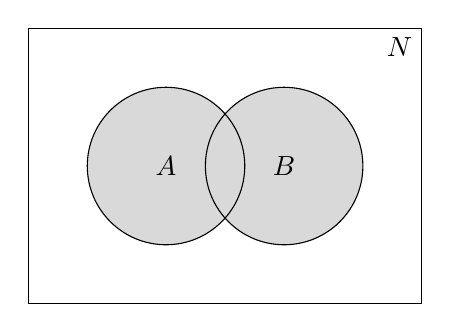
\begin{tikzpicture}

    % Rectangle with label
    \draw (0,0) rectangle (5,3.5) node[below left] {$\mathbb{N}$};
    
    \fill[gray!30] (1.75,1.75) circle (1);
    \fill[gray!30] (3.25,1.75) circle (1);

    \node[draw, circle, minimum width=2cm, label=center:{$A$}] at (1.75, 1.75) {};
    \node[draw, circle, minimum width=2cm, label=center:{$B$}] at (3.25, 1.75) {};

\end{tikzpicture}
\caption{\label{fig:Venn-diagram}Representation of $A \cup B$ as a Venn Diagram}
\end{figure}

Given any two sets $A$ and $B$, the \emph{set difference}\index{Set difference} is denoted by $A \backslash B$, and the \emph{complement}\index{Complement of a set} of the set $A$ is written as $A^c$. \emph{De Morgan's laws}\index{De Morgan's laws} state that for any sets $A$ and $B$, we have $\left( A \cup B \right)^c = A^c \cap B^c$ and $\left( A \cap B \right)^c = A^c \cup B^c$.

Two sets $A$ and $B$ are said to be \emph{disjoint}\index{Disjoint sets} if their intersection is empty, i.e., $A \cap B = \varnothing$. A collection of sets $A_1, A_2, \ldots, A_n$ is disjoint if $A_i \cap A_j = \varnothing$ for all $i \neq j$. A \emph{partition}\index{Partition of a set} of a set $A$ is a collection of nonempty, pairwise disjoint subsets $A_1, A_2, \ldots, A_n$ such that $A = \cup_{i=1}^n A_i$. The \emph{power set}\index{Power set} of $A$, denoted by $\mathcal{P}(A)$, is the set of all possible subsets of $A$. If the cardinality of $A$ is $n$, i.e., $d(A) = n$, then the cardinality of its power set is $2^n$, so $d\left( \mathcal{P}(A) \right) = 2^n$.

\begin{example}
Given the set $A = \{1, 2, 3\}$, its power set is:
\[
\mathcal{P}(A) = \{\varnothing, \{1\}, \{2\}, \{3\}, \{1,2\}, \{1,3\}, \{2,3\}, A\}
\]
\end{example}

Consider a non-empty set $A$ and a collection $\mathcal{F}$ of subsets of $A$. The pair $\left( A, \mathcal{F} \right)$ is called a \emph{field}\index{Field of sets} over $A$ if it satisfies the following conditions: it contains the empty set, that is, $\varnothing \in \mathcal{F}$; it is closed under complementation, meaning that for every $F \in \mathcal{F}$, the complement $F^c$ also belongs to $\mathcal{F}$; and it is closed under finite unions, meaning that for any subsets $F_1, \ldots, F_n \in \mathcal{F}$, the union $F_1 \cup \ldots \cup F_n$ is also in $\mathcal{F}$. Additionally, it can be shown that a field also satisfies two further properties: the universal set $A$ itself belongs to $\mathcal{F}$, and it is closed under finite intersections, so that $F_1 \cap \ldots \cap F_n \in \mathcal{F}$ for all subsets $F_1, \ldots, F_n \in \mathcal{F}$.

% Relations

Consider two elements, $x$ and $y$. An \emph{ordered pair}\index{Ordered pair}, denoted as $(x, y)$, is a pairing in which the order of the elements matters. Generalizing this idea, an \emph{n-tuple}\index{n-tuple} is an ordered sequence of $n$ elements, written as $(x_1, \ldots, x_n)$. The \emph{Cartesian product}\index{Cartesian product} of two sets $A$ and $B$, denoted by $A \times B$, is the set of all ordered pairs $(x, y)$ such that $x \in A$ and $y \in B$. This concept extends naturally to $n$ sets $A_1, A_2, \dots, A_n$, where the Cartesian product is expressed as $A_1 \times A_2 \times \dots \times A_n$. Additionally, the \emph{n-fold Cartesian product} of a set $A$ with itself is denoted as $A^n$.

Let $R$ be a subset of the Cartesian product of a set $A$ with itself, i.e., $R \subseteq A \times A$. Such a subset is called a \emph{binary relation}\index{Binary relation}. We write $aRb$ to indicate that the ordered pair $(a, b)$ belongs to $R$. A binary relation is said to be \emph{reflexive}\index{Reflexive relation} if, for every element $a \in A$, it holds that $aRa$. It is called \emph{symmetric}\index{Symmetric relation} if, for all $a, b \in A$, the condition $aRb$ implies $bRa$. A relation is \emph{antisymmetric}\index{Antisymmetric relation} if, for all $a, b \in A$, the coexistence of $aRb$ and $bRa$ implies $a = b$. It is \emph{transitive}\index{Transitive relation} if, for all $a, b, c \in A$, the conditions $aRb$ and $bRc$ together imply $aRc$. A relation is \emph{total}\index{Total relation} if, for every pair $a, b \in A$, either $aRb$ or $bRa$ holds. Binary relations can also be defined between two different sets $A$ and $B$, in which case $R$ is a subset of $A \times B$. Furthermore, the concept can be generalized to \emph{n-ary} relations, represented as $R \subseteq A_1 \times A_2 \times \dots \times A_n$.

Let $R$ be a binary relation that is a subset of the Cartesian product $A \times A$, i.e., $R \subseteq A \times A$. If this relation is reflexive, symmetric, and transitive, it is called an \emph{equivalence relation}\index{Equivalence relation}, typically denoted by the symbol $\sim$. Under an equivalence relation, two elements $a, b \in A$ are said to be \emph{equivalent}\index{Equivalent elements} if $a \sim b$. The \emph{equivalence class}\index{Equivalence class} of an element $a$, denoted by $[a]$, is the set of all elements in $A$ that are equivalent to $a$. That is, the equivalence class of $a$ is defined as $[a] := \{ b \in A : a \sim b \}$. An equivalence relation partitions the set $A$ into disjoint subsets known as \emph{equivalence classes}, collectively forming what is called the \emph{quotient set}\index{Quotient set}. The quotient set is denoted by $A / {\mathord {\sim }}$ and is defined as the set of all equivalence classes: $A / {\mathord {\sim }} := { [a] : a \in A }$.

A binary relation that is reflexive, transitive, and antisymmetric is known as a \emph{partial order}\index{Partial order}, typically denoted by the symbol $\preceq$. A set equipped with a partial order is called a \emph{partially ordered set}\index{Partially ordered set}, or \emph{poset}\index{poset} for short. In a poset, an element $a \in A$ is considered \emph{minimal}\index{Minimal element} if there is no element $b \in A$ such that $b \preceq a$ and $b \neq a$. Similarly, an element $a$ is said to be \emph{maximal}\index{Maximal element} if there is no element $b \in A$ such that $a \preceq b$ and $b \neq a$. A relation that is reflexive, transitive, antisymmetric, and total is called a \emph{total order}\index{Total order}, often denoted by the symbol $\leq$. A set endowed with a total order is referred to as a \emph{totally ordered set}\index{Totally ordered set}. In such a set $A$, the \emph{maximum element}\index{Maximum element}, denoted by $\max(A)$, satisfies $\max(A) \geq x$ for all $x \in A$, and the \emph{minimum element}\index{Minimum element}, denoted by $\min(A)$, satisfies $\min(A) \leq x$ for all $x \in A$.

\begin{example}
Let $R$ be a relation that is a subset of the Cartesian product of the set of natural numbers $\mathbb{N}$ with itself, i.e., $R \subset \mathbb{N} \times \mathbb{N}$. In this relation, an ordered pair $(a, b)$ belongs to $R$ if and only if $a$ is a divisor of $b$. The set $\mathbb{N}$, together with the relation $R$, forms a partially ordered set. In this context, 1 is the unique minimal element, and every prime (e.g. 11) is maximal.
\end{example}

% Functions

A \emph{function}\index{Function} is defined as a binary relation $f \subseteq A \times B$ such that for each element $x \in A$, there exists at most one $y \in B$ for which $\left(x, y\right) \in f$. In this context, elements $\left(x, y\right) \in f$ are written as $f(x) = y$, and the function is denoted by $f : A \rightarrow B$. The set $A$ is called the \emph{domain}\index{Domain} of $f$, and $B$ is the \emph{codomain}\index{Codomain}. The set ${ y \in B : \exists x \in A \text{ such that } f(x) = y }$ is known as the \emph{range}\index{Range} of $f$. If the relation is not defined for every $x \in A$, the function is called a \emph{partial function}\index{Partial function}, and we write $f(x) \uparrow$ to indicate that $f$ is undefined at $x$.

A function is said to be \emph{injective}\index{Injective function} if, for all elements $x$ and $y$, the condition $f(x) = f(y)$ implies that $x = y$. A function is \emph{surjective}\index{Surjective function} if, for every $y$ in the codomain, there exists at least one $x$ in the domain such that $f(x) = y$. A function is described as \emph{bijective}\index{Bijective function} if it is both injective and surjective. The \emph{identity}\index{Identity function} function $I_A : A \rightarrow A$, defined by $I_A(a) = a$ for all $a \in A$, is an example of a bijective function. These concepts (function, partial function, injective, surjective, and bijective) can be extended to $n$-ary functions, which are functions of the form $f: A_1 \times A_2 \times \dots \times A_n \rightarrow B$.

The \emph{inverse}\index{Inverse function} of a bijective function $f$, denoted by $f^{-1}$, is defined as $f(f^{-1}(x)) = f^{-1}(f(x)) = x$, for all $x$ in the domain of $f^{-1}$ and the range of $f$, respectively. Given two functions $f$ and $g$, where the domain of $f$ includes the range of $g$, the \emph{composition}\index{Composition} of $f$ with $g$, denoted by $f \circ g$, is defined as $(f \circ g)(x) = f(g(x))$.

\begin{example}
In Section \ref{sec:computable_functions}, we will explore an alternative interpretation of a function as a procedure or algorithm that assigns an element of $B$ to each element of $A$. For example, the following C code defines a partial function from $\mathbb{R}$ to $\mathbb{R}$, which is partial because $inv(0) \uparrow$:
\begin{verbatim}
    double inv(double x) {
        return 1 / x;
    }
\end{verbatim}
\end{example}

The \emph{characteristic function}\index{Characteristic function} of a set $A$ is denoted by $1_A : A \rightarrow \{1, 0\}$, where $1_A(x) = 1$ if $x \in A$ and $1_A(x) = 0$ otherwise.

An infinite set $A$ is said to be \emph{countable}\index{Countable set} if there exists a bijective function that maps the elements of $A$ onto the set of natural numbers $\mathbb{N}$. In contrast, a set is considered \emph{uncountable}\index{Uncountable set} if it is neither finite nor countable. A set is said to have \emph{countably many}\index{Countably many set} elements if it is either finite or countably infinite.

\begin{example}
The sets $\mathbb{N}$, $\mathbb{Z}$, and $\mathbb{Q}$ are countable, whereas $\mathbb{R}$ is uncountable.
\end{example}

Considering a real number $x \in \mathbb{R}$, its \emph{absolute value}\index{Absolute value}, denoted by $\mid x \mid$, is defined as $x$ if $x \geq 0$ and $-x$ if $x < 0$. The \emph{ceiling}\index{Ceil} function of $x$, written as $\lceil x \rceil$, is the smallest integer greater than or equal to $x$. The \emph{floor}\index{Floor} function of $x$, denoted by $\lfloor x \rfloor$, is the largest integer less than or equal to $x$. Given two positive integers $a$ and $b$, the \emph{modulo}\index{Modulo} operation, written as $a \bmod b$, yields the remainder when $a$ is divided by $b$.

For two functions $f$ and $g$ defined as $f, g : \mathbb{N} \rightarrow \mathbb{R}^{+}$, we say that $f(n)$ is of the \emph{order of}\index{Order of a function} $g(n)$, denoted $f(n) = O(g(n))$, if there exist positive constants $c > 0$ and $m$ such that $f(n) \leq c g(n)$ for all integers $n \geq m$. In this context, $g$ is called an \emph{upper bound}\index{Upper bound of a function} for $f$.

%
% Section: Strings and Languages
%

\section{Strings and Languages}
\label{sec:strings}

Consider a non-empty finite set $\mathcal{S} = \{ s_1, s_2, \ldots, s_q \}$, referred to as the \emph{alphabet}\index{Alphabet}. The elements of this set are called \emph{symbols}\index{Symbols}. A \emph{sequence}\index{Sequence of symbols} over $\mathcal{S}$ is defined as an ordered arrangement of symbols $x_1 x_2 \dots x_n$, where each $x_i$ belongs to $\mathcal{S}$. In the special case where the alphabet is $\mathcal{B} = \{0, 1\}$, such sequences are known as \emph{binary sequences}\index{Binary sequence}. We use the term \emph{string}\index{String} to denote a finite sequence. This book primarily focuses on binary strings.

The \emph{length}\index{Length of a string} of a string $s$, denoted by $l(s)$, refers to the total number of symbols contained in $s$. The symbol $\lambda$ is used to denote the \emph{empty string}\index{Empty string}, which is defined as the unique string over $\mathcal{S}$ with length 0. Given a symbol $x \in \mathcal{S}$, the string consisting of $x$ repeated $n$ times is denoted by $x^n$. If $s = x_1 x_2 \dots x_n$ is a string, its \emph{reverse}\index{Reverse string}, denoted by $s^R$, is given by $x_n x_{n-1} \dots x_1$.

The set of all strings $s\_{1}s\_{2}\ldots s\_{n}$ of length $n$ over the alphabet $\mathcal{S}$ is denoted by $\mathcal{S}^{n}$\footnote{It is important to avoid confusing the set of strings of length $n$ over an alphabet, $\mathcal{S}^n$, with the $n$-fold Cartesian product of a set, $S^n$. The use of calligraphic fonts helps distinguish between alphabets and other sets.}. We denote by $\mathcal{S}^{+}$ the union of all $\mathcal{S}^{n}$ for $n \geq 1$, and by $\mathcal{S}^{\ast}$ the set $\mathcal{S}^{+} \cup {\lambda}$. Note that all strings in $\mathcal{S}^{\ast}$ have finite length. The term \emph{Kleene closure}\index{Kleene closure} refers to $\mathcal{S}^{\ast}$.

\begin{example}
The following relations hold: the cardinality of the set of binary strings of length $n$ is $d \left( \left\{ s \in \mathcal{B}^{\ast} : l(s) = n \right\} \right) = 2^n$, and the cardinality of the set of binary strings of length up to $n$ is $d \left( \left\{ s \in \mathcal{B}^{\ast} : l(s) \leq n \right\} \right) = 2^{n+1}-1$.
\end{example}

Given two strings $s$ and $t$ from $\mathcal{S}^{\ast}$, the \emph{concatenation}\index{String concatenation} of $s$ and $t$, denoted as $st$, is the sequence obtained by placing the sequence of symbols in $t$ immediately after the sequence in $s$. Consequently, the length of the concatenated string, $l(st)$, is the sum of the lengths of $s$ and $t$. This indicates that $\mathcal{S}^\ast$ is closed under the operation of concatenation. Moreover, the set $\mathcal{S}^\ast$, together with concatenation, forms a \emph{free monoid}\index{Free monoid}. This means that concatenation is associative ($s(tr) = (st)r$), and that there exists an identity element, specifically, the empty string $\lambda$, for which $\lambda a = a \lambda = a$ holds for any string $a$.

A string $s$ is called a \emph{substring}\index{Substring} of a string $t$ if there exist strings $u$ and $v$ (possibly empty) such that $t = usv$. If there exists a string $u$ such that $t = su$, then $s$ is said to be a \emph{prefix}\index{Prefix string} of $t$, denoted by $s <_p t$. A subset $S \subset \mathcal{S}^{\ast}$ is described as \emph{prefix-free}\index{Prefix free set} if, for any $s, t \in S$, the condition $s <_p t$ implies $s = t$. Given two sets of strings $S, T \subset \mathcal{S}^{\ast}$, the (left) \emph{quotient}\index{String quotient} $S^{-1}T$ is defined as the set of residual strings obtained from $T$ by removing a prefix in $S$; formally, $S^{-1}T = \{\, t \mid st \in T \land s \in S \,\}$.

We denote the \emph{self-delimited}\index{Self delimited string} form of a string $s \in \mathcal{S}^{\ast}$ by $\bar{s}$, and define it as $\bar{s} = 1^{l(s)}0s$. Consequently, the length of $\bar{s}$, denoted $l(\bar{s})$, is given by $l(\bar{s}) = 2l(s) + 1$, meaning it is twice the length of $s$ plus one.

\begin{example}
The set $\bar{\mathcal{S}^{\ast}}$, consisting of all self-delimited strings from $\mathcal{S}^{\ast}$, is prefix-free.
\end{example}

In cases where $\mathcal{S}$ is a totally ordered set, we can define a total order on $\mathcal{S}^{\ast}$. This ordering, known as \emph{shortlex ordering}\index{Shortlex ordering}, arranges sequences primarily by length, with shorter sequences appearing first. Among sequences of the same length, lexicographical order is used to break ties.

\begin{example}
Given $\mathcal{S} = {a, b, c}$ with $a < b < c$, the shortlex order on $\mathcal{S}^{\ast}$ produces the sequence $\lambda < a < b < c < aa < ab < \ldots < cc < aaa < aab < \ldots < ccc < \ldots$
\end{example}

For any arbitrary object $O$, we use the notation $\left\langle O \right\rangle$ to denote its string based representation, assuming the existence of a standard encoding scheme. For objects $O_{1}, O_{2}, \ldots, O_{k}$, the expression $\left\langle O_1 O_2 \ldots O_k \right\rangle$ refers to the plain concatenation of their string representations: $\left\langle O_1 \right\rangle \left\langle O_2 \right\rangle \ldots \left\langle O_k \right\rangle$. By contrast, the notation $\left\langle O_1, O_2, \ldots, O_k \right\rangle$ indicates a structured concatenation that allows for the decoding and unique identification of each individual object. For example, this may be implemented as $\bar{\left\langle O_1 \right\rangle} \bar{\left\langle O_2 \right\rangle} \ldots \bar{\left\langle O_k \right\rangle}$.

\begin{example}
Natural numbers can be represented by binary strings via the following encoding method: $\langle 0 \rangle = \lambda$, $\langle 1 \rangle \rightarrow 0$, $\langle 2 \rangle \rightarrow 1$, $\langle 3 \rangle \rightarrow 00$, $\langle 4 \rangle \rightarrow 01$, $\langle 5 \rangle \rightarrow 10$, $\langle 6 \rangle \rightarrow 11$, $7 \rightarrow 000$, and so on. Therefore, the pair of numbers $\left\langle 3, 7 \right\rangle$ would be represented as $110001110000$. Given this particular encoding, it follows that $l \left( \langle n \rangle \right) = \lfloor \log_2 (n + 1) \rfloor$.
\end{example}

A \emph{language}\index{Language}, denoted by $L$, over an alphabet $\mathcal{S}$, is defined as a subset of strings, that is, $L \subseteq \mathcal{S}^{\ast}$. The individual elements of $L$ are called \emph{words}\index{Words of a language}. The unique language that contains no words is referred to as the \emph{empty language}\index{Empty language}, and is denoted by $L = \varnothing$.

Consider two languages $L_1$ and $L_2$ over a common alphabet $\mathcal{S}$. Several standard operations can be applied to these languages. The \emph{union} of $L_1$ and $L_2$ is defined as $L_1 \cup L_2 = { w \in \mathcal{S}^{\ast} \mid w \in L_1 \text{ or } w \in L_2 }$. The \emph{intersection} of $L_1$ and $L_2$ is given by $L_1 \cap L_2 = { w \in \mathcal{S}^{\ast} \mid w \in L_1 \text{ and } w \in L_2 }$. The \emph{complement} of $L_1$ is defined as $\overline{L_1} = { w \in \mathcal{S}^{\ast} \mid w \notin L_1 }$. Finally, the \emph{Kleene closure} of $L_1$, denoted $L_1^\ast$, is defined as $L_1^\ast = { \lambda } \cup { wz \mid w \in L_1 \text{ and } z \in L_1^\ast }$.

Languages can be systematically generated using a finite set of string rewriting rules, commonly referred to as grammars. A \emph{grammar}\index{Grammar}, denoted by $G$, is defined as a 4-tuple $(N, \Sigma, P, S)$, where: $N \subseteq \mathcal{S}$ is a finite set of \emph{nonterminal symbols}\index{Non-terminal symbol}; $\Sigma \subseteq \mathcal{S}$ is a finite set of \emph{terminal symbols}\index{Terminal symbol}; $P$ is a finite set of \emph{production rules}\index{Production rule} of the form $(\Sigma \cup N)^\ast N (\Sigma \cup N)^\ast \rightarrow (\Sigma \cup N)^\ast$; and $S \in N$ is a distinguished \emph{start symbol}\index{Start symbol}. Each production rule allows one string of symbols to be rewritten into another, beginning with the start symbol and proceeding through successive applications of the rules.

\begin{example}
\label{ex:context_free_grammar}
Consider the alphabet $\mathcal{S} = \{ S, a, b \}$, and define the grammar $(N, \Sigma, P, S)$ where $N = \{ S \}$, $\Sigma = \{ a, b \}$, $P = \{ S \rightarrow aSb, S \rightarrow ba \}$, and the start symbol is $S \in N$. This grammar generates the language $L = \{ a^nbab^n \mid n\geq0 \} = \{ ba, abab, aababb, aaababbb, \ldots \}$.
\end{example}

The \emph{Chomsky hierarchy}\index{Chomsky hierarchy} is a classification scheme for grammars, organized according to their expressive power, that is, the types of languages they are capable of generating. The hierarchy, arranged from the most to the least restrictive class of grammars, is described as follows (where $a$ denotes a terminal symbol; $A, B$ are nonterminal symbols; and $\alpha, \beta$, and $\gamma$ are strings composed of terminals and/or nonterminals):

\begin{description}
\item[Type-3] Known as \emph{regular grammars}\index{Regular grammar}. In these grammars, the left-hand side of each production rule consists of a single nonterminal symbol. The right-hand side must be either the empty string, a single terminal symbol, or a terminal symbol followed by a nonterminal symbol. Formally, the rules are of the form $A \rightarrow \lambda$, $A \rightarrow a$, or $A \rightarrow aB$.

\item[Type-2] Referred to as \emph{context-free grammars}\index{Context-free grammar}. In this class, the left-hand side of each production rule is exactly one nonterminal symbol. The general form of the rules is $A \rightarrow \alpha$.

\item[Type-1] These are \emph{context-sensitive grammars}\index{Context sensitive grammar}. Here, production rules allow a nonterminal to be replaced by a string in a specific context. The rules take the form $\alpha A \beta \rightarrow \alpha \gamma \beta$.

\item[Type-0] This category includes \emph{recursively enumerable grammars}\index{Recursively enumerable grammar}, which place no restrictions on the structure of production rules. These can be written in the general form $\gamma \rightarrow \alpha$.
\end{description}

\begin{example}
The grammar presented in Example \ref{ex:context_free_grammar} is a Type-2 grammar, that is, a context-free grammar.
\end{example}

The \emph{Backus-Naur form}\index{Backus-Naur form} (BNF) is a notation system specifically designed to describe context-free grammars. It is widely used in computer science to formally specify the syntax of programming languages and communication protocols. A BNF grammar consists of a set of production rules structured as follows:

\begin{verbatim}
    <symbol> ::= __expression__
\end{verbatim}

Here, \texttt{<symbol>} denotes a non-terminal symbol, \texttt{\_\_expression\_\_} represents a sequence of terminal and/or non-terminal symbols, and \texttt{::=} signifies that the symbol on the left-hand side can be replaced by the expression on the right. Multiple alternatives for the expression can be provided in a single rule by separating them with a vertical bar \texttt{|}, indicating that any one of the alternatives may be chosen during substitution. Symbols that never appear on the left-hand side of any production rule are considered terminal symbols. In contrast, those that do appear on the left-hand side are non-terminal symbols and are conventionally enclosed in angle brackets \texttt{<>}. The non-terminal symbol on the left-hand side of the first production rule is designated as the start symbol.

\begin{example}
The grammar introduced in Example \ref{ex:context_free_grammar} can be expressed in Backus-Naur form using the following production rule:
\begin{verbatim}
    <string> ::= a <string> b | ba
\end{verbatim}
\end{example}

%
% Section: Counting Methods
%

\section{Counting Methods}
\label{sec:counting}

\emph{Combinatorics}\index{Combinatorics}, a specialized branch of mathematics, is primarily concerned with the study of discrete objects and the relationships among them. Its central themes include the counting, arrangement, and selection of such objects, along with the methods used to carry out these tasks. Combinatorics provides a powerful set of tools for analyzing large collections of objects that satisfy specific properties. In this section, we revisit the most important results in combinatorics, focusing on their interpretation in terms of sets and ordered lists.

The \emph{multiplication rule}\index{Multiplication rule} is a fundamental principle that determines the number of possible outcomes in the Cartesian product of sets. According to this rule, if there are $k$ sets $A_1, A_2, \ldots, A_k$, and each set $A_i$ contains $n_i$ elements (for $i = 1, \ldots, k$), then the Cartesian product $A_1 \times A_2 \times \ldots \times A_k$ contains exactly $n_1 n_2 \ldots n_k$ elements. In particular, if a set $A$ has $n$ elements, then the $k$-fold Cartesian product $A^k$ contains $n^k$ elements.

The \emph{inclusion-exclusion principle}\index{Inclusion-exclusion principle} determines the cardinality of the union of multiple sets based on the sizes of the individual sets and all possible intersections among them. Given $k$ sets $A_1, A_2, \ldots, A_k$, the formula is:
\begin{equation*}
\begin{split}
d \left( \bigcup_{i=1}^k A_i \right) & = \sum_{i=1}^k d \left( A_i \right) - \sum_{i<j} d \left( A_i \cap A_j \right) + \sum_{i<j<l} d \left( A_i \cap A_j \cap A_l \right) - \\
& - \sum_{i<j<l<m} d \left( A_i \cap A_j \cap A_l \cap A_m \right) + \ldots +  (-1)^{k+1} d \left( A_1 \cap \ldots \cap A_k \right) 
\end{split}
\end{equation*}
\emph{Permutations}\index{Permutations} refer to the number of distinct ways in which the elements of a set can be arranged. Let $A$ be a set with $n$ elements. The number of ordered selections of $k$ elements from $n$ distinct elements without replacement, denoted by $P_{n,k}$, is given by $P_{n,k} = n \left( n-1 \right) \ldots \left( n-k+1 \right)$. In the case where $k = n$, the total number of permutations is $P_{n,n} = n \left( n-1 \right) \cdots 1 = n!$ where $n!$ is read as "$n$ factorial".

\begin{example}
Consider the set $\{a, b, c\}$. There are six distinct permutations of its elements: $\{a, b, c\}$, $\{a, c, b\}$, $\{b, a, c\}$, $\{b, c, a\}$, $\{c, a, b\}$, and $\{c, b, a\}$. Each permutation represents a unique ordering of the elements in the original set.
\end{example}

The \emph{pigeonhole principle}\index{Pigeonhole principle} is a simple yet powerful concept. It asserts that if there are more pigeons than pigeonholes, then at least one pigeonhole must contain more than one pigeon. More formally, if $n$ items are distributed among $m$ containers and $n > m$, then at least one container must hold more than one item.

The logarithmic form of \emph{Stirling's}\index{Stirling's formula} approximation is particularly effective for estimating large factorials:
\[
\log\left(n!\right) \approx \frac{1}{2}\log\left(2\pi\right)+\left(n+\frac{1}{2}\right)\log\left(n\right)-n
\]

Numerous counting problems involve determining the number of subsets of a specific size within a given set. For a set with $n$ elements, the total number of possible subsets is $2^n$, including both the empty set and the set itself. The number of subsets of size $k$, also known as the number of \emph{combinations}\index{Combinations} of $k$ elements from a set of $n$, is denoted by $C_{n,k}$ and computed using the formula $C_{n,k} = \frac{P_{n,k}}{k!} = \frac{n!}{k!(n-k)!}
$. The symbol ${n \choose k}$ also represents the value $C_{n,k}$, which is known as the \emph{binomial coefficient}\index{Binomial coefficient}. It is known that ${n \choose 0} = {n \choose n} = 1$ for all $n$, and ${n \choose k} = {n \choose n-k}$ for all $k = 0, 1, \ldots, n$. Additionally, ${n \choose k} = 0$ whenever $k > n$.

\begin{example}
Consider the set $\{a, b, c, d\}$. There are 4 combinations of size 3: $[a, b, c]$, $[a, b, d]$, $[a, c, d]$, and $[b, c, d]$. Since combinations disregard order, $[a, c, d]$ and $[d, c, a]$ represent the same combination.
\end{example}

The \emph{multinomial coefficient}\index{Multinomial coefficient}, a generalization of the binomial coefficient to more than two categories, represents the number of ways to partition a set of objects into a fixed number of subsets, each containing a specified number of elements. Suppose we have a set with $n$ elements that is to be divided into $k$ subsets of sizes $n_1, n_2, \ldots, n_k$, respectively. The multinomial coefficient, denoted as ${n \choose n_{1}, n_{2},\ldots, n_{k}}$, gives the number of such possible partitions and is calculated by the formula:
\[
{n \choose n_{1},n_{2},\ldots,n_{k}} = \frac{n!}{n_{1}!n_{2}!\ldots n_{k}!}
\]
where $n_1 + n_2 + \cdots + n_k = n$.

The different combinations of replacement and ordering lead to four distinct counting scenarios, as summarized below. These conditions depend on whether the order of selection matters and whether elements can be selected more than once.
\begin{center}
\begin{tabular}{ c c c }
& Without replacement & With replacement \\
Ordered    & $\frac{n!}{(n-r)!}$ & $n^r$ \\
Unordered  & $\binom{n}{r}$      & $\binom{n+r-1}{r}$
\end{tabular}
\end{center}
In the first row, we consider ordered selections: without replacement, the number of ways corresponds to the number of permutations of $r$ elements from a set of $n$; with replacement, each of the $r$ positions can independently be filled with any of the $n$ elements. In the second row, we consider unordered selections: without replacement, the count is given by the standard binomial coefficient; with replacement, the result corresponds to the number of multisets of size $r$ formed from $n$ distinct elements.

%
% Section: Matrices
%

\section{Matrices}

A \emph{matrix}\index{Matrix}, denoted by $A$, of order $m \times n$ is a rectangular array consisting of $m$ \emph{rows} and $n$ \emph{columns}, filled with a sequence of $mn$ scalars. It is typically written as:
\[
A = 
 \begin{pmatrix}
  a_{1,1} & a_{1,2} & \cdots & a_{1,n} \\
  a_{2,1} & a_{2,2} & \cdots & a_{2,n} \\
  \vdots  & \vdots  & \ddots & \vdots  \\
  a_{m,1} & a_{m,2} & \cdots & a_{m,n} 
 \end{pmatrix}
\]

The \emph{entry} $a_{ij}$ denotes the element located at the $i$-th row and $j$-th column of the matrix $A$. The \emph{set of all matrices} of order $m \times n$ is denoted by $\mathcal{M}_{m \times n}$. A \emph{row matrix}\index{Row matrix} is any matrix in the set $\mathcal{M}_{1 \times n}$, while a \emph{column matrix}\index{Column matrix} belongs to $\mathcal{M}_{m \times 1}$. A \emph{square matrix}\index{Square matrix} is an element of $\mathcal{M}_{n \times n}$. The entries $a_{ii}$ of a square matrix form its \emph{main diagonal}\index{Matrix main diagonal}. A \emph{diagonal matrix}\index{Diagonal matrix} is a square matrix in which all entries outside the main diagonal are zero. The \emph{identity matrix}\index{Identity matrix}, denoted by $I$, is a special diagonal matrix with all diagonal entries equal to 1.

The \emph{transpose}\index{Matrix transpose} of a matrix $A \in \mathcal{M}_{m \times n}$ is defined as the matrix $A^T \in \mathcal{M}_{n \times m}$, whose entry at position $(i,j)$ is equal to the entry at position $(j,i)$ in $A$. If $A = A^T$, then $A$ is called a \emph{symmetric matrix}\index{Symmetric matrix}. A \emph{submatrix}\index{Submatrix} of a matrix is obtained by deleting one or more rows and/or columns.

\begin{example}
Consider the square matrix $A = \left( \begin{smallmatrix} 1 & 2 & 3 \\ 4 & 5 & 6 \\ 7 & 8 & 9 \end{smallmatrix} \right)$. The entry in position $(2, 3)$ is $6$, and the main diagonal consists of the elements $1$, $5$, and $9$. The transpose of $A$ is $A^T = \left( \begin{smallmatrix} 1 & 4 & 7 \\ 2 & 5 & 8 \\ 3 & 6 & 9 \end{smallmatrix} \right)$. The matrix $B = \left( \begin{smallmatrix} 1 & 3 \\ 4 & 6 \end{smallmatrix} \right)$ is a submatrix of \$A\$.
\end{example}

The addition of two matrices $A$ and $B$ of the same size produces a new matrix $A + B$, where each entry at position $(i, j)$ is defined as $(A + B)_{ij} = a_{ij} + b_{ij}$. Matrix addition is associative, i.e., $(A + B) + C = A + (B + C)$, and commutative, i.e., $A + B = B + A$. It has a neutral element, the zero matrix, such that $A + 0_{m \times n} = A$, and each matrix has an additive inverse, since $A + (-A) = 0_{m \times n}$.

The product of a scalar $\lambda$ and a matrix $A$ yields another matrix, denoted by $\lambda A$, in which each entry at position $(i, j)$ is given by $(\lambda A)_{ij} = \lambda a_{ij}$. Scalar multiplication is distributive over matrix addition, i.e., $\lambda (A + B) = \lambda A + \lambda B$, and over scalar addition, i.e., $(\alpha + \beta) A = \alpha A + \beta A$. It is also associative with respect to scalar multiplication, i.e., $(\alpha \beta) A = \alpha (\beta A)$, and has a multiplicative identity, since $1 A = A$.

The product of two matrices $A_{m \times n}$ and $B_{n \times p}$ results in a matrix $AB_{m \times p}$, where each entry at position $(i, j)$ is given by $(AB)_{ij} = \sum_{k=1}^n a_{ik} b_{kj}$. Matrix multiplication is associative, meaning that $(AB)D = A(BD)$. It has a left identity element: $AI_n = A$, and a right identity element: $I_mA = A$. It is also compatible with scalar multiplication, so that $\alpha(AB) = (\alpha A)B = A(\alpha B)$. Furthermore, matrix multiplication is distributive over addition: from the right, $A(B + C) = AB + AC$, and from the left, $(B + C)D = BD + CD$.

The transpose operation satisfies the following properties: $(A + B)^T = A^T + B^T$, $(\lambda A)^T = \lambda A^T$, and $(AB)^T = B^T A^T$.

\begin{example}
Given the matrices $A = \left( \begin{smallmatrix} 1 & 2 \\ 3 & 5 \end{smallmatrix} \right)$ and $B = \left( \begin{smallmatrix} 5 & 6 \\ 7 & 8 \end{smallmatrix} \right)$ we have that $A + B = \left( \begin{smallmatrix} 6 & 8 \\ 10 & 13 \end{smallmatrix} \right)$, $2 A = \left( \begin{smallmatrix} 2 & 4 \\ 6 & 10 \end{smallmatrix} \right)$ and $A B = \left( \begin{smallmatrix} 19 & 22 \\ 50 & 58 \end{smallmatrix} \right)$.
\end{example}

A square matrix $A$ is said to be \emph{invertible} or \emph{non-singular}\index{Non-singular matrix} if there exists a matrix $B$ such that $AB = BA = I$. If $A$ is non-singular, the matrix $B$ is unique and is called the \emph{inverse} of $A$, denoted by $A^{-1}$. A matrix $A$ is called \emph{orthogonal}\index{Orthogonal matrix} if its transpose is equal to its inverse, that is, $A^T = A^{-1}$. The columns and rows of an orthogonal matrix are referred to as \emph{orthonormal vectors}\index{Orthonormal vector}.

The \emph{determinant}\index{Matrix determinant} is a special scalar value that can be computed from the elements of a square matrix. For a matrix $A$, the determinant is denoted by $\det(A)$. It can be calculated using the Leibniz formula:
\[
\det(A) = \sum_{\sigma \in S_n} \operatorname{sgn}(\sigma) \cdot a_{1,\sigma(1)} \cdot a_{2,\sigma(2)} \cdots a_{n,\sigma(n)}
\]
where $S_n$ denotes the set of all permutations of the integers $1$ to $n$, and $\operatorname{sgn}(\sigma)$ is the sign of the permutation $\sigma$, equal to $+1$ for even permutations and $-1$ for odd permutations. A matrix is invertible if and only if its determinant is nonzero.

\begin{example}
The determinant of a $3 \times 3$ matrix $A = \left( \begin{smallmatrix} a & b & c \\ d & e & f \\ g & h & i \end{smallmatrix} \right)$ is computed as:
\[
\det(A) = aei + bfg + cdh - ceg - bdi - afh
\]
\end{example}

For a given matrix $A$, the \emph{rank}\index{Matrix rank}, denoted as $\operatorname{rank}(A)$, is the maximum number of linearly independent rows or columns in the matrix.

A number $\lambda$ and a nonzero vector $\mathbf{v}$ such that $A \mathbf{v} = \lambda \mathbf{v}$ are called an \emph{eigenvalue}\index{Eigenvalue} and an \emph{eigenvector}\index{Eigenvector} of $A$, respectively.

Matrix decomposition is the process of transforming a matrix into a more tractable form while preserving certain properties, such as the determinant or rank. The \emph{singular value decomposition}\index{Singular value decomposition} (SVD) of a matrix $A$ of order $m \times n$ is a factorization of the form $A = U \Sigma V^T$, where $U$ is an $m \times m$ orthogonal matrix, $\Sigma$ is an $m \times n$ diagonal matrix with nonnegative entries, and $V^T$ is the transpose of an $n \times n$ orthogonal matrix.

%
% Section: Graphs
%

\section{Graphs}
\label{sec:Graphs}

A \emph{graph}\index{Graph}\footnote{The definition of a graph stated here corresponds to the definition of a \emph{simple graph} as found in typical discrete mathematics literature.} $G$ is represented as an ordered pair $(V,E)$, comprising a set $V$, referred to as \emph{vertices}\index{Vertices of a graph}, and a set $E$, denoted as \emph{edges}\index{Edges of a graph}. The members of $E$ take the form of unordered pairs $\left\{ u,v\right\}$, constituting distinct vertices $u,v\in V$ (loops are not permitted). Vertices $u$ and $v$ are described as \emph{adjacent}\index{Adjacent vertices} when an edge $\left\{ u,v\right\} \in E$ exists, consequently, they are termed the \emph{endpoints}\index{Endpoints of an edge} of that edge. If the set $V$ is infinite, the graph is classified as an \emph{infinite graph}\index{Infinite graph}. This book, however, focuses exclusively on finite graphs. Given that $G = (V,E)$ is a graph, its \emph{adjacency matrix}\index{Adjacency matrix} is a square $d(V) \times d(V)$ matrix $A$ whereby element $A_{uv}$ equals 1 if $\left\{ u,v\right\} \in E$ and 0 otherwise.

Graphs are typically illustrated as a collection of dots representing vertices, linked by lines denoting edges.

\begin{example}
\label{ex:binary_tree}
If $V=\{a, b, c, d\}$ and $E=\{ \{a,b\}, \{a,c\}, \{a,d\}, \{b,c\} \}$, the graph $G=(V,E)$ is represented in Figure \ref{fig:Graph-Example}.
\end{example}

\begin{figure}[t]
\centering
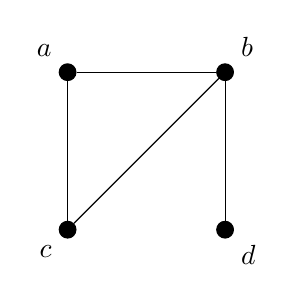
\begin{tikzpicture}

  % Small circles
  \node[draw, fill=black, circle, inner sep=0.075cm, label=above left:{$a$}] (circlea) at (0, 0) {};
  \node[draw, fill=black, circle, inner sep=0.075cm, label=above right:{$b$}] (circleb) at (2, 0) {};
  \node[draw, fill=black, circle, inner sep=0.075cm, label=below left:{$c$}] (circlec) at (0, -2) {};
  \node[draw, fill=black, circle, inner sep=0.075cm, label=below right:{$d$}] (circled) at (2, -2) {};

  % Arrows
  \draw[-] (circlea) to (circleb);
  \draw[-] (circlea) to (circlec);
  \draw[-] (circleb) to (circled);
  \draw[-] (circleb) to (circlec);

\end{tikzpicture}
\caption{\label{fig:Graph-Example}An Example of Graph}
\end{figure}

When a vertex $v$ serves as an endpoint of an edge $e$, it is said that $e$ is \emph{incident}\index{Incident edge} upon $v$. The \emph{degree}\index{Degree of a vertex} of a vertex $v$, notated as $\deg(v)$, corresponds to the count of edges incident on $v$. A vertex with degree zero is labeled as \emph{isolated}\index{Isolated vertex}, while a vertex with degree one is termed \emph{pendant}\index{Pendant vertex}. The \emph{neighborhood}\index{Neighborhood of a vertex} of a vertex $v$, signified by $N(v)$, includes all vertices that are adjacent to $v$. If $A \subset V$, the neighborhood of $A$ is given by $N(A) = \cup_{v \in A} N(v)$. A \emph{path}\index{Path} in a graph consists of a series of unique vertices $\{v_{0}, v_{1}, \ldots ,v_{k}\}$ such that $v_{i}$ and $v_{i+1}$ are adjacent for each $1 \leq i < k$. A path is known as a \emph{simple path}\index{Simple path} if no vertex is repeated. A graph is considered \emph{connected}\index{Connected graph} when a path exists between any two vertices. If $v_{0} = v_{k}$, the path is defined as a \emph{cycle}\index{Cycle}. A cycle is called a \emph{simple cycle}\index{Simple cycle} if it consists of at least three vertices and only the first and last vertices are repeated. 

\begin{example}
In a given graph $G=(V,E)$, the \emph{handshaking theorem}\index{Handshaking theorem} posits that $\sum_{v \in V} \deg(v) = 2m$, where $m = d(E)$, given that each edge has two endpoints.
\end{example}

If the vertex pairs $u, v$ are arranged in ordered pairs, the graph is termed a \emph{directed graph}\index{Directed graph}. In this case, $u$ is referred to as the \emph{initial vertex}\index{Initial vertex}, while $v$ is known as the \emph{terminal vertex}\index{Terminal vertex}. Given that $G$ is a directed graph, the \emph{in-degree}\index{In-degree of a vertex} of a vertex $v$, signified by $indeg(v)$, corresponds to the count of edges in which $v$ serves as a terminal vertex. The \emph{out-degree}\index{Out-degree of a vertex}, denoted by $outdeg(v)$, refers to the number of edges where $v$ is the initial vertex. A directed graph is \emph{strongly connected}\index{Strongly connected graph} if a directed path connects each pair of vertices. Directed graphs are typically illustrated with arrows, rather than lines, to represent edges.

A graph $G$ is classified as \emph{bipartite}\index{Bipartite graph} if the vertex set $V$ can be partitioned into two subsets $V_1$ and $V_2$ such that every edge of $G$ links a vertex from $V_1$ to one from $V_2$. Bipartite graphs are usually denoted as $G=(V_1, V_2, E)$. The degree of vertices in a bipartite graph adheres to the \emph{degree sum formula}\index{Degree sum formula}, $\sum_{u \in V_1} \deg(u) = \sum_{v \in V_2} \deg(v) = d(E)$.

A graph $G(V',E')$ is a \emph{subgraph}\index{Subgraph} of $G(V,E)$ if $V'$ is a subset of $V$ and $E'$ is a subset of $E$ with endpoints that belong to $V'$. A graph $G$ is termed a \emph{labeled graph}\index{Labeled graph} if its edges and/or vertices are assigned specific data. Specifically, if each edge $e$ of $G$ is allocated a nonnegative number $w(e)$, then $w(e)$ is referred to as the \emph{weight}\index{Weight of an edge} of $e$.

A specific type of graph that plays a fundamental role in this book is the \emph{tree}\index{Tree}. Defined as a non-empty graph, a tree ensures any pair of vertices are interconnected by a singular, unique path. A tree always includes a specially designated vertex termed the \emph{root}\index{Root of a tree}, and every edge of the tree is oriented away from the root.

\begin{example}
An alternative definition of trees, based on set theory, posits that a tree is a partially ordered set $(T, <)$ such that for each $t \in T$, the set $S = \{ s \in T : s < t \}$ possesses a least element – an element smaller than all other elements in $S$.
\end{example}

Given a tree $T$, for any vertex $v$ other than the root, the \emph{parent}\index{Parent of a vertex} of $v$ is the single, unique vertex $u$ such that an edge directly links $u$ to $v$. Conversely, if $u$ is the parent of $v$, $v$ is then identified as a \emph{child}\index{Child of a vertex} of $u$. Any other vertex within the tree sharing the same parent as $v$ is considered a \emph{sibling}\index{Sibling to a vertex} of $v$. The \emph{ancestors}\index{Ancestors of a vertex} of a vertex encompass all vertices along the path from the root to the given vertex, excluding the vertex itself but including the root. The \emph{descendants}\index{Descendant of a vertex} of a vertex $v$ include those vertices that count $v$ as an ancestor. A vertex with no children is labeled as a \emph{leaf}\index{Leaf vertex}, whereas vertices possessing children are referred to as \emph{branches}\index{Branches of a tree}. The \emph{depth}\index{Depth of a vertex} of a vertex $v$ is determined by the length of the unique path leading from the root to $v$. The \emph{height}\index{Height of a tree} of a tree is the maximum among the depths of all its vertices.

\begin{example}
For the tree illustrated in Figure \ref{fig:BinaryTree-Example}, the root vertex is $a$; $c$ serves as a parent of $d$, making $d$ a child of $c$; $d$ and $g$ are siblings; the ancestors of $d$ include $a$ and $c$; the descendants of $c$ comprise $d$, $e$, and $f$; leaf nodes in the tree are $b$, $e$, $f$, and $g$; $a$ and $c$ are branches; the depth of $d$ is 3; the height of the tree is 4.
\end{example}

\begin{figure}[t]
\centering
\begin{tikzpicture}

  % Small circles
  \node[draw, circle, inner sep=0.2cm, label=center:{$a$}] (circlea) at (0, 0) {};
  \node[draw, circle, inner sep=0.2cm, label=center:{$b$}] (circleb) at (-2, -2) {};
  \node[draw, circle, inner sep=0.2cm, label=center:{$c$}] (circlec) at (2, -2) {};
  \node[draw, circle, inner sep=0.2cm, label=center:{$d$}] (circled) at (0, -4) {};
  \node[draw, circle, inner sep=0.2cm, label=center:{$g$}] (circleg) at (4, -4) {};
  \node[draw, circle, inner sep=0.2cm, label=center:{$e$}] (circlee) at (-2, -6) {};
  \node[draw, circle, inner sep=0.2cm, label=center:{$f$}] (circlef) at (2, -6) {};


  % Arrows
  \draw[-] (circlea) to (circleb);
  \draw[-] (circlea) to (circlec);
  \draw[-] (circlec) to (circled);
  \draw[-] (circlec) to (circleg);
  \draw[-] (circled) to (circlee);
  \draw[-] (circled) to (circlef);

\end{tikzpicture}
\caption{\label{fig:BinaryTree-Example}An Example of a Tree}
\end{figure}

Given a vertex $v$ in a tree, the \emph{subtree}\index{Subtree} with $v$ as its root is the subgraph within the tree that includes $v$, its descendants, and all edges connected to these descendants. A tree is termed a \emph{k-ary tree}\index{k-ary tree} if each branch houses no more than $k$ children. If every branch comprises exactly $k$ children, the tree is then labeled a \emph{full k-ary tree}\index{full k-ary tree}. A \emph{k-ary} tree where $k=2$ is specifically referred to as a \emph{binary tree}\index{Binary tree}. A $k$-ary tree of height $h$ is deemed \emph{balanced}\index{Balanced tree} if all its leaves are located at a depth of $h$ or $h-1$.

\begin{example}
A tree composed of $n$ vertices includes $n-1$ edges. A full $k$-ary tree featuring $i$ branches hosts $m=ki+1$ vertices.
\end{example}

The procedure of visiting each node in a tree exactly once is defined as \emph{tree traversal}\index{Tree traversal}. The classifications of tree traversals are determined by the order of node visits, namely, \emph{depth-first} and \emph{breadth-first} order. In a depth-first traversal\index{Depth-first tree traversal}, the algorithm initiates at the root node and ventures as far as possible along each branch before transitioning to the next sibling. There are three standard strategies for processing nodes within the tree: \emph{in-order}\index{In-order tree traversal}, \emph{pre-order}\index{Pre-order tree traversal}, and \emph{post-order}\index{Post-order tree traversal}.

The following snippet of code, resembling C language syntax, demonstrates the usage of a recursive pre-order depth-first traversal algorithm to print a binary tree:

\begin{verbatim}
    void print_tree(binary_tree *tree) {
        if (!is_empty(tree)) {
            printf("%c\n",tree->node); /* print node */
            print_tree(tree->left_branch); /* process left branch */
            print_tree(tree->right_branch); /* process right branch */
        }
    }
\end{verbatim}

Conversely, in a breadth-first traversal\index{Breadth-first tree traversal}, the algorithm commences at the tree root and explores all nodes at the current depth before progressing to nodes at the subsequent depth level. Implementing depth-first tree traversal algorithms necessitates the employment of sophisticated data structures. For an example of such algorithms, please consult the references section.

\begin{example}
In the case of the tree delineated in Example \ref{ex:binary_tree}, a pre-order depth-first traversal would yield the string "abcdefg". Conversely, a pre-order breadth-first traversal would generate the string "abcdgef".
\end{example}

%
% Section: References
%

\section*{References}

The book "Discrete Mathematics" by Johnsonbaugh \cite{johnsonbaugh2009discrete} is tailored for undergraduate students taking a one- or two-semester course in discrete mathematics, thoroughly covering key topics in the field. "Introduction to the Theory of Computation" by Sipser \cite{sipser2012introduction} offers a comprehensive, clear, and student-centric introduction to the latest computational theory topics and methodologies. It is highly acclaimed for its in-depth exploration of automata, formal languages, and complexity theory. "Introduction to Algorithms" by Cormen et al. \cite{cormen1990introduction}, commonly known by the acronym "CLRS" derived from the authors' initials, is a seminal work in the algorithms field, encompassing a broad spectrum of topics, including graph algorithms. This book is both extensive and rigorous. Finally, "Matrix Computations" by Golub and Van Loan \cite{golub2013matrix} delves into various topics related to matrices, with an emphasis on matrix computations - an area of particular interest to those engaged in computational studies.








%
% CHAPTER: Descriptive Statistics
%

% %
% CHAPTER: Probability Theory
%

\chapterimage{owl} % Chapter heading image

\chapter{Descriptive Statistics}
\label{chap:descriptive_statistics}

\begin{quote}
\begin{flushright}
\emph{Pending}\\
Thomas Bayes
\end{flushright}
\end{quote}
\bigskip


Statistics involves the methods used for collecting, organizing, summarizing, presenting, and analyzing data. It also focuses on drawing valid conclusions and making informed decisions based on this analysis. Statistics typically does not deals with unusual or rare cases.

Rather than studying an entire population, statistics examines a smaller subset known as a sample. When a sample accurately represents a population, significant insights about the population can often be deduced from the sample analysis. The branch of statistics that addresses the conditions under which such deductions are valid is known as inductive statistics, or statistical inference. Since these inferences are not completely certain, probabilistic language is commonly employed when presenting conclusions. Conversely, the branch of statistics that solely aims to describe and analyze a specific group, without making any broader conclusions or inferences, is referred to as descriptive statistics.

{\color{red} TODO: Extend}

%
% Section: Descriptive Statistics
%

\section{Descriptive Statistics}

Statistics is a field that revolves around the collection, analysis, and interpretation of data. At the heart of statistical analysis is the concept of a population, which is fundamental in understanding how data reflects a group of interest. 

\begin{definition}
Let $\mathcal{S}$ be a set referred to as the \emph{population}\index{Population}. Its constituents are termed \emph{individuals}\index{Individual}.
\end{definition}

The set $\mathcal{S}$ must be well-defined, non-empty, and it can be either finite or infinite. 

A variable is a symbol used to represent the characteristics or attributes of individuals within a population. It is called 'variable' because these attributes can vary from one individual to another, although from a pure mathematical perpective the term function might have been more appropriate.

\begin{definition}
Let $\mathcal{S}$ be a population, and let $\mathcal{D}$ be the set containing all possible values that the individuals of $\mathcal{S}$ can assume. A variable $X$ is a function $X: \mathcal{S} \rightarrow \mathcal{D}$ that maps individuals from the population $\mathcal{S}$ to the values in $\mathcal{D}$.
\end{definition}

The set $\mathcal{D}$ can be any set, such as the real numbers, a set of integers, or a set of categorical labels. A variable is called a \emph{quantitative variable}\index{Quantitative variable} if it the elements of $\mathcal{S}$ can be measured numerically. These can be further classified as \emph{discrete variables}\index{Discrete variable} if they can take a countable number of distinct values, and \emph{continuous variables}\index{Continuous variable} if they can take any value within a given range or interval. A variable is called a \emph{qualitative}\index{Qualitative variable} or \emph{categorical variable}\index{Categorical variable} if it represents quantities that cannot be measured numerically. A qualitative variable can be a \emph{nominal variable}\index{Nominal variable} if no natural order exists among the categories, or an \emph{ordinal variable}\index{Ordinal variable} if a natural order exists among the categories.

\begin{example}
Consider a population consisting of the inhabitants of a small village, where we are interested in studying three attributes of these individuals: age, gender, and daily water consumption. The variable representing age, mapping individuals to their ages in years, is a quantitative discrete variable because it can be counted precisely in integer values. Gender, mapping individuals to categories like "Male" or "Female," is a qualitative nominal variable because the categories have no inherent order. Finally, daily water consumption, mapping individuals to the amount of water they drink in liters, is a quantitative continuous variable as it can take any real number within a range, reflecting precise measurements.
\end{example}

% Frequency distributions

\section{Frequency Distributions}

When summarizing large masses of raw data, it is often useful to distribute the data into classes, or categories, and to determine the number of individuals belonging to each class, called absolute frequency. The following definition formally introduces this concept.

\begin{definition}
Let $\mathcal{S}$ be a population consisting of $n$ individuals, and let a variable $X: \mathcal{S} \rightarrow \mathcal{D}$ represent the mapping of individuals in $\mathcal{S}$ to values in the set $\mathcal{D}$, where $k$ is the cardinality of $\mathcal{D}$. The \emph{absolute frequency}\index{Absolute frequency}, also known simply as \emph{frequency}, denoted by $n_i$ for $1 \leq i \leq k$, quantifies the number of individuals in $\mathcal{S}$ for which $X$ assigns the value corresponding to the $i$-th category of $\mathcal{D}$.
\end{definition}

The sum of the frequencies must be equal to population size, that is, $\sum_{i=1}^k n_i = n$.

If the variable $X$ is continuous, the elements of $\mathcal{D}$ are referred to as \emph{class intervals}\index{Class interval}. The endpoints of these intervals are known as \emph{class limits}\index{Class limits}; the smaller number is termed the \emph{lower class limit}\index{Lower class limit}, and the larger number, the \emph{upper class limit}\index{Upper class limit}. A \emph{class interval}\index{Class interval} that lacks either an upper or a lower class limit is known as an \emph{open class interval}\index{Open class interval}. The \emph{width}\index{Class interval width} of a class interval is defined as the difference between the upper and lower class boundaries, denoted by $a_i = e_i - e_{i-1}$. The \emph{class mark}\index{Class mark}, or the midpoint of a class interval, is calculated as $a_i = \frac{e_i + e_{i-1}}{2}$. It is assumed that all observations within a specific class interval are equivalent concerning their categorical assignment. Refer to Section \ref{sec:discretization_algorithms} for more information about how to discretize a continous variable into discrete intervals.

\begin{example}
In a study measuring adult heights within a community, researchers record heights ranging from 150 cm to 200 cm and organize them into 10 cm class intervals: 150-159 cm, 160-169 cm, 170-179 cm, 180-189 cm, and 190-199 cm. Each interval's lower and upper class limits are respectively the start and end points, such as 150 cm and 159 cm for the first interval. If the last interval had no specified upper limit, it would be considered an open class interval. The class width, typically 10 cm, is the operational span between boundaries, and the class mark, calculated as the midpoint of each interval (e.g., 154.5 cm for the first interval), provides a central value for summarizing data within that range.
\end{example}

A tabular arrangement of data by classes together with the corresponding class frequencies is called a frequency distribution, or frequency table.

\begin{definition}
Let $\mathcal{S}$ be a population consisting of $n$ individuals, and let $X: \mathcal{S} \rightarrow \mathcal{D}$ be a variable that maps individuals in $\mathcal{S}$ to $k$ distinct values of the set $\mathcal{D}$. A \emph{frequency distribution}\index{Frequency distribution} is represented the set of pairs $\{(d_i, n_i) : 1 \leq i \leq k\}$, where $d_i$ denotes the $i$-th interval and $n_i$ represents the number of individuals from $\mathcal{S}$ whose value under $X$ falls within the interval $d_i$.
\end{definition}

Frequency distributions are useful for statistical analysis and helps in visualizing data by grouping values, which simplifies the understanding of distribution and central tendencies within the data.

The relative frequency of a class is the frequency of the class divided by the total frequency of all classes

\begin{definition}
Let $\mathcal{S}$ be a population consisting of $n$ individuals, and let a variable $X: \mathcal{S} \rightarrow \mathcal{D}$ represent the mapping of individuals in $\mathcal{S}$ to values in the set $\mathcal{D}$, where $k$ is the cardinality of $\mathcal{D}$. The \emph{relative frequency}\index{Relative frequency}, denoted by $f_i$, is the ratio $f_i = \frac{n_i}{n}$ for $1 \leq i \leq k$.
\end{definition}

The sum of the relative frequencies is equal to one, that is, $\sum_{i=1}^k f_i = 1$.

The total frequency of all values less than the upper class boundary of a given class interval is called the cumulative frequency up to and including that class interval.

\begin{definition}
Let $\mathcal{S}$ be a population consisting of $n$ individuals, and let a variable $X: \mathcal{S} \rightarrow \mathcal{D}$ represent the mapping of individuals in $\mathcal{S}$ to values in the set $\mathcal{D}$, where $k$ is the cardinality of $\mathcal{D}$. The \emph{cumulative frequency}\index{Cumulative frequency}, denoted by $N_i$ for $1 \leq i \leq k$, represents the total number of individuals in $\mathcal{S}$ for which $X$ assigns a value less than or equal to the upper limit of the $i$-th category of $\mathcal{D}$. This is mathematically expressed as $N_i = \sum_{j=1}^i n_j$, where $n_j$ is the absolute frequency of the $j$-th category.
\end{definition}

By accumulating the frequencies up to each category or interval, cumulative frequencies provides a running total that shows how many data points fall below a certain value.

%
% Section: Characterizing Distributions
%

\section{Characterizing Distributions}
\label{sec:measures_central_tendency}

A \emph{measure of central tendency} is a number derived from a population, intended as a summary of that population. The most common measures of central tendency in use are the mode, the median and the mean. Each of these measures provides a different approach to characterize populations. It is also common to use \emph{metrics of dispersion} to describe the variability of a frequency distribution around the measures of centrality. We will review two metrics of dispersion, the variance and the standard deviation. All these measures allow us to summarize and compare populations.

% The Mean

\subsection*{Mean}

The most commonly used measure of central tendency is the \emph{mean}. The mean of a population is the weighted average of the distinct values of the individuals in the population, where weights are given by the frequencies.

\begin{definition}
\label{def:mean}
Let $X$ be a variable representing the mapping of the $N$ individuals of a population $\mathcal{S}$ to the set of possible values $\mathcal{D} = \{x_1, x_2, \dots, x_k\}$, each occurring with frequency $\{n_1, n_2, \dots, n_k\}$ and relative frequency $\{f_1, f_2, \dots, f_k\}$. The \emph{mean}\index{mean} of $X$, denoted by $\overline{X}$, is defined as:
\[
\overline{X} = \frac{1}{N} \sum_{i=1}^k n_i x_i = \sum_{i=1}^k f_i x_i
\]
\end{definition}

Definition \ref{def:mean} can be directly applied to the case of quantitative discrete variables, but it requires some considerations in the case of continuous variables. For continuous cases, we could use the average of the observed values. That is, if for individuals $s_1, \ldots, s_N$ we have observed the values $y_1, \ldots, y_N$ for the characteristic of interest, the mean would be given by:
\[
\overline{X} = \frac{1}{N} \sum_{i=1}^N y_i 
\]
Alternatively, we could group the observed values into a reduced number of intervals. In that case, the mean could be computed as the weighted average of the class marks $a_1, \ldots, a_k$:
\[
\overline{X} = \frac{1}{N} \sum_{i=1}^k n_i a_i
\]
We must be careful about the number of intervals, as it is described in Section \ref{sec:discretization_algorithms}.

The mean, while widely used as a measure of central tendency, has several notable limitations. First and foremost, it is not suitable for categorical variables, where numerical operations such as averaging are not meaningful. In such cases, the mode is typically used as a more appropriate measure of central tendency. Another limitation of the mean is that it may not correspond to an actual value observed in the dataset, particularly in datasets with wide ranges or unusual distributions. This can make the mean less representative of typical values in the dataset. Furthermore, the mean is sensitive to outliers or extreme values; even a small change in the frequency of a large number in the set $\mathcal{D}$ can disproportionately affect the mean, potentially skewing analysis. This sensitivity makes the mean less robust compared to other measures, such as the median, which is less influenced by outliers and extreme data points.

\begin{example}
Consider a small company with a population of 10 employees, and that th characteristic in which we are interetes is their salaries. Let's $\mathcal{D} = \{50, 300\}$ with  frequencies of $9$ and $1$ respectively. The mean salary is calculated as:
\[ 
\overline{X} = \frac{(50 \times 9) + (300 \times 1)}{10} = \frac{450 + 300}{10} = 75
\]
Now, suppose the executive receives a raise or another executive with the same high salary joins the company, making two employees earning \$300,000. The recalculated mean salary would be:
\[
\overline{X} = \frac{(50 \times 8) + (300 \times 2)}{10} = \frac{400 + 600}{10} = 100
\]
This example shows how just a small change, a single additional person earning a significantly higher salary, can substantially increase the mean salary from \$75,000 to \$100,000.
\end{example}

The preference for the mean over other measures of central tendency such as the median or mode is primarily due to its mathematical properties that facilitate algebraic manipulations and further statistical analysis. For example, the mean is linear, which means that the mean of a linear transformation of a variable is the same transformation applied to the mean of the variable.

\begin{proposition}
Let $X_1, \ldots, X_n$ be $n$ variables with means $\overline{X}_1, \ldots, \overline{X}_n$, and let $a_1, \ldots, a_n$ and $b$ constants. The mean of a linear combination of the variables $X' = a_1 X_1 + \ldots + a_n X_n + b$ is given by
\[
\overline{X}' = a_1 \overline{X}_1 + \ldots + a_n \overline{X}_n + b
\]
\end{proposition}
\begin{proof}
{\color{red} TODO: Review}
We have that
\begin{multline}
\overline{X}' = \sum_{x_1} \ldots \sum_{x_n} \left(a_ 1 x_1 + \ldots + a_n x_n + b  \right) f\left(x_1, \ldots, x_n \right) = \\
\sum_{x_1} \ldots \sum_{x_n} a_1 x_1 f\left(x_1, \ldots, x_n \right) + \ldots + \sum_{x_1} \ldots \sum_{x_n} a_n x_n f\left(x_1, \ldots, x_n \right) + \sum_{x_1} \ldots \sum_{x_n} b f\left(x_1, \ldots, x_n \right) = \\
\sum_{x_1} a_1 x_1 f\left(x_1\right) + \ldots + \sum_{x_n} a_n x_n f\left( x_n \right) + b = 
a_1 \sum_{x_1} x_1 f\left(x_1\right) + \ldots + a_n \sum_{x_n} x_n f\left( x_n \right) + b = \\
a_1 \overline{X}_1 + \ldots + a_n \overline{X}_n + b
\end{multline}
\end{proof}

% The Median

\subsubsection*{The Median}
\label{sec:median}

The median represents the middle value in a population when the individuals are arranged in order given a characteristic. This measure is particularly valuable because it provides a clear indication of the central location of the data, especially in cases where the population may be skewed or contain outliers. The median is often favored over the mean in these situations because it is less sensitive to extreme values, making it a more robust indicator of the population's typical value.

The formal definition of the median in statistics can be articulated as follows:

\begin{definition}
The \emph{median} of a dataset is the value that separates the higher half of the data from the lower half. For a dataset \( X = \{x_1, x_2, \dots, x_n\} \) sorted in ascending order, the median \( M \) is defined as:
\[
M = \begin{cases} 
x_{\left(\frac{n+1}{2}\right)} & \text{if } n \text{ is odd} \\
\frac{x_{\left(\frac{n}{2}\right)} + x_{\left(\frac{n}{2}+1\right)}}{2} & \text{if } n \text{ is even}
\end{cases}
\]
\end{definition}

The advantages of the meadian are: robustness against outliers, unlike the mean, the median is not significantly affected by extreme values or skewed data, providing a more accurate reflection of the typical value; useful for ordinal data, the median can be calculated for ordinal data where the mean cannot be meaningfully computed. Its disadvantages include: limited sensitivity to data changes, small changes in data near the median do not affect its value, while changes at the ends of the dataset might not have any effect unless they shift the median position; more complex calculation for large datasets, unlike the mode, which is simply the most frequent value, calculating the median involves sorting the data, which can be computationally intensive for large datasets.

\begin{example}
Consider a real estate agent analyzing home prices in a neighborhood where the prices are: \$100,000, \$150,000, \$160,000, \$170,000, \$200,000, \$600,000, \$900,000. Sorting the prices in ascending order gives: \$100,000, \$150,000, \$160,000, \$170,000, \$200,000, \$600,000, \$900,000. Since there are seven data points, the median (middle value) is \$170,000. This median price gives a more accurate reflection of the typical home price than the mean, which is skewed by the two high prices.
\end{example}

The median of a population remains invariant under any monotonic transformation, meaning if the population undergoes a transformation that preserves the order of data points, the position of the median remains unchanged.

\begin{proposition}
Let \( X = \{x_1, x_2, \dots, x_n\} \) be a dataset with median \( M \). For any monotonically increasing function \( f \), the dataset \( Y = \{f(x_1), f(x_2), \dots, f(x_n)\} \) has the median \( f(M) \).
\end{proposition}
\begin{proof}
Given that \( f \) is monotonically increasing, the order of the data points is preserved. Therefore, the middle value of \( Y \) after applying \( f \) is simply \( f \) applied to the median of \( X \), which is \( f(M) \).
\end{proof}

% The Mode

\subsubsection*{The Mode}
\label{sec:mode}

The mode is a measure of central tendency often described as the most frequently occurring value in a population. It is particularly significant because it provides a direct indication of the most common category or value in a population. This makes the mode especially useful in analyzing categorical data where numerical measures like mean and median are not applicable.

The formal definition of mode in statistics can be expressed as follows:

\begin{definition}
The \emph{mode} of a dataset is the value that appears most frequently in the dataset. For a dataset \( X = \{x_1, x_2, \dots, x_n\} \), the mode \( M \) is defined such that the frequency of \( M \) is greater than the frequency of any other value in \( X \).
\end{definition}

The most relevant advantages of the mod are: it is simple to understand and easy to compute, it is useful for categorical data where numerical averages cannot be computed, and it is insensitive to extreme values, unlike the mean, which makes it stable in the presence of outliers. However, it also present some disadvantages, including that it is not uniquely defined, if two or more values appear with the same highest frequency, leading to a dataset having multiple modes or being bimodal or multimodal, and it is less informative, about the dataset as a whole compared to the mean or median, especially in numeric data.

\begin{example}
Suppose a teacher wants to determine the most common score on a test where the grades are: 85, 92, 85, 97, 85, 92, 92, 84. The score 85 occurs three times, and the score 92 also occurs three times. Hence, this dataset is bimodal with modes at 85 and 92, indicating these scores were the most common.
\end{example}

The mode is invariant under scale transformations.

\begin{proposition}
Let \( X = \{x_1, x_2, \dots, x_n\} \) be a dataset with mode \( M \). For any real number \( a \neq 0 \) and \( b \), the dataset \( Y = \{a x_1 + b, a x_2 + b, \dots, a x_n + b\} \) has the mode \( aM + b \).
\end{proposition}
\begin{proof}
Since multiplying and adding constants to each element in \( X \) maintains the relative frequency of the values, the transformed version of \( M \) will appear with the same frequency in dataset \( Y \), thus, \( aM + b \) is the mode of \( Y \).
\end{proof}

%
% Measures of Dispersion
%
\subsection{Measures of Dispersion}

Definitions of the Variance and the Standard Deviation

\begin{definition}
Let X be a random variable with finite mean and $\mu=E\left(X\right)$. The variance of X, denoted by $Var\left(X\right)$, is defined as follows: $Var\left(X\right)=E\left[\left(X-\mu^{2}\right)\right]$
\end{definition}

{\color{red} If X has infinite mean or if the mean of X does not exist, we say that $Var\left(X\right)$ does not exist. The standard deviation of X is the nonnegative square root of $Var\left(X\right)$ if the variance exists. It is common to denote the standard deviation by the symbol $\sigma$, and the variance by $\sigma^{2}$. Variance depeds only on the distribution.}

\begin{proposition}
For every random variable X, $Var\left(X\right)=E\left(X^{2}\right)-\left[E\left(X\right)\right]^{2}$.
\end{proposition}
\begin{proof}
\end{proof}

{\color{red} The variance (as well as the standard deviation) of a distribution provides a measure of the spread or dispersion of the distribution around its mean $\mu$. The variance of a distribution, as well as its mean, can be made arbitrarily large by placing even a very small but positive amount of probability far enough from the origin on the real line.}

Properties of the Variance

\begin{proposition}
For constants a and b, let $Y=aX+b$, then $Var\left(Y\right)=a^{2}Var\left(X\right)$
and $\sigma_{Y}=\left|a\right|\sigma_{X}$.
\end{proposition}
\begin{proof}
\end{proof}

{\color{red} If $X_{\text{1}},\ldots,X_{n}$ are independent random variables with finite means, and if $a_{1},\ldots,a_{n}$ and b are arbitrary constants, then $Var\left(a_{1}X_{1}+\ldots+a_{n}X_{n}+b\right)=a_{1}^{2}Var\left(X_{1}\right)+\ldots+a_{n}^{2}Var\left(X_{n}\right)$}

\begin{example}
The Variance of a Binomial Distribution

The variance of a random variable X with a binomial distribution of n samples with probability p is $Var\left(X\right)=np\left(1-p\right)$
\end{example}


%
% Measures fo Statistical Relationship
%

\section{Measures of Statistical Relationship}
\label{sec:measures_statistical_relationship}

The metrics of disperson can also be used in case of bivariate distributions, under the names of covariance and correlation, to measure the \emph{statistical relationship} between two random variables.

Covariance and correlation are attempst to measure the linear dependence between to random variables.

Covarance

\begin{definition}
Definition 183. Let X and Y be random variables having finite means. Let $E\left(X\right)=\mu_{X}$ and $E\left(Y\right)=\mu_{Y}$. The covariance of X and Y, which is denoted by $Cov\left(X,Y\right)$ is defined as $Cov\left(X,Y\right)=E\left[\left(X-\mu_{X}\right)\left(Y-\mu_{Y}\right)\right]$
\end{definition}

if the expectation exists.

The covariance between X and Y is intended to measre the degree to which X and Y tend to be large at the same time or the degree to which one tends to be large while the other is small.

\begin{proposition}
For all random variables X and Y such that $\sigma_{X}^{2}<\infty$ and $\sigma_{Y}^{2}<\infty Cov\left(X,Y\right)=E\left(XY\right)-E\left(X\right)E\left(Y\right)$
\end{proposition}
\begin{proof}
\end{proof}

Correlation

Correlation is a measure of association between two random variables that is not driven by arbitrary changes in the scales.

\begin{definition}
Let X and Y be random variables with finite variances $\sigma_{X}^{2}$ and $\sigma_{Y}^{2}$ respectively. Then the correlation of X and Y, which is denoted by $\rho\left(X,Y\right)$, is defined as follows $\rho\left(X,Y\right)=\frac{Cov\left(X,Y\right)}{\sigma_{X}\sigma_{Y}}$
\end{definition}

XX

\begin{definition}
It is said that X and Y are positively correlated if $\rho\left(X,Y\right)>0$, that X and Y are negatively correlated if $\rho\left(X,Y\right)<0$ and that X and Yare uncorrelated if $\rho\left(X,Y\right)=0$.
\end{definition}

Properties of Covariance and Correlation

\begin{proposition}
Moreover $-1 \leq \rho\left(X,Y\right) \leq 1$
\end{proposition}
\begin{proof}
\end{proof}

\begin{proposition}
If X and Y are independent random variables with $0<\text{\ensuremath{\sigma_{X}^{2}}}<\infty$ and $0<\text{\ensuremath{\sigma_{Y}^{2}}}<\infty$ then $Cov\left(X,Y\right)=\rho\left(X,Y\right)=0$
\end{proposition}
\begin{proof}
\end{proof}

The converse is not true as a general rule. Two dependent random variables can be uncorrelated.

\begin{proposition}
Suppose that X is a random variable such that $0<\sigma_{X}^{2}\infty$ and $Y=aX+b$ for some constants a and b, where $a\neq0$. If $a>0$ then $\rho\left(X,Y\right)=1$. If $a<0$, then $\rho\left(X,Y\right)=-1$.
\end{proposition}
\begin{proof}
\end{proof}

The converse is also true, that is, if $\left|\rho\left(X,Y\right)\right|=1$ implies that X and Y are linearly related.

\begin{proposition}
If X and Y are random variables such that $Var\left(X\right)<\infty$ and $Var\left(Y\right)<\infty$, then $Var\left(X+Y\right)=Var\left(X\right)+Var\left(Y\right)+2Cov\left(X,Y\right)$
\end{proposition}
\begin{proof}
\end{proof}

For all constants a and b, it can be shown that $Cov\left(aX,bY\right)=abCov\left(X,Y\right)$.

\begin{proposition}
Let X and Y are random variables such that $Var\left(X\right)<\infty$ and $Var\left(Y\right)<\infty$, and let a, b and c be constants, then $Var\left(aX+bY+c\right)=a^{2}Var\left(X\right)+b^{2}Var\left(Y\right)+2abCov\left(X,Y\right)$
\end{proposition}
\begin{proof}
\end{proof}

A special case is $Var\left(X-Y\right)=Var\left(X\right)+Var\left(Y\right)-2Cov\left(X,Y\right)$

\begin{proposition}
If $X_{1},\ldots,X_{n}$ are random variables such that $Var\left(X_{i}\right)<\infty for i=1,\ldots,n$, then $Var\left(\sum_{i=1}^{n}X_{i}\right)=\sum_{i=1}^{n}Var\left(X_{i}\right)+2\sum\sum Cov\left(X_{i},X_{j}\right)$
\end{proposition}
\begin{proof}
\end{proof}

\begin{proposition}
If $X_{1},\ldots,X_{n}$ are uncorrelated random variables, then $Var\left(\sum_{i=1}^{n}X_{i}\right)=\sum_{i=1}^{n}Var\left(X_{i}\right)$
\end{proposition}
\begin{proof}
\end{proof}


%
% Section: Common Distribution
%

\section{Common Distributions}
\label{sec:probability_distributions}


\subsection{Uniform Distribution}

\begin{definition}
Let $a \leq b$ be integers. Suppose that the value of a random variable $X$ is equally likely to be each of the integers $a, \ldots, b$. Then we say that $X$ has the uniform distribution on the integers $a, \ldots, b$.
\end{definition}

{\color{red} Introduce the following propostion}

\begin{proposition}
If $X$ has the uniform distribution on the integers $a,\ldots,b$, the p.f. of $X$ is $f\left(x\right)=\begin{cases}
\frac{1}{b-a+1} & for\,x=a,\ldots,b\\
0 & otherwise
\end{cases}$
\end{proposition}
\begin{proof}
\end{proof}

{\color{red} The uniform distribution on the integers $a, \ldots, b$ represents the outcome of an experiment that is often described by saying that one of the integers $a, \ldots, b$ is chosen at random. A uniform distribution cannot be assigned to an infinite sequence of possible values}


\subsection{Bernoulli Distributions}

\begin{example}
A random variable $Z$ that takes only two values $0$ and $1$ with $P\left(Z=1\right)=p$ has the Bernoulli distribution with parameter $p$. We also say that $Z$ is a Bernoulli random variable with parameter $p$.
\end{example}

\subsection{Binomial Distributions}

\begin{example}
Suppose we perform $N$ independent trials where each trial either succeeds or fails with probability of success $p$, and let $X$ the random variable defined by the number of successes. The probability of having exactly $n$ successes $P(X=n)$ follows a \emph{binomial distribution} with parameters $N, p$, defined by:
\[
f(n\mid N, p) = \binom{N}{n} p^n (1-p)^{(N-n)}
\]
\end{example}

\begin{definition}
The discrete distribution represented by the p.f.f $\left(x\right)=\begin{cases}
{n \choose x}p^{x}\left(1-p\right)^{n-x} & for\,x=0,1,\ldots,n\\
0 & otherwise
\end{cases}$
\end{definition}

{\color{red} is called the binomial distribution with parameters $n$ and $p$.}

{\color{red} Consider a general experiment that consists of observing $n$ independent trials with only two possible results for each trial: success and failure. Then the distribution of the number of trials that result in success will be binomial with parameters $n$ and $p$, where $p$ is the probability of success on each trial.} 

%
% Section: Discretization of Continuous Data
%

\section{Discretization of Continuous Variables}
\label{sec:discretization_algorithms}

{\color{red} TODO: Rewrite this section.}

Let $\mathcal{X}$ a continuous random variable that follows a probability density function $P_\mathcal{X}$, and assume we have collected $n$ independent and identically distributed samples $\bold{x} = \{x_1, \ldots, x_n\}$ from $\mathcal{X}$. We are interested in computing the length of a compressed version of $\bold{x}$ using an optimal compressor. Unfortunately, and except for some degenerate distributions, there is no lossless compression algorithm that produces a string with fewer bits than encoding directly the elements $\bold{x}$. Compression algorithms for continuous data only work in case that the elements of $\bold{x}$ are not independent, as it is the case with images or sound. But, if this is not the case, the only option available to compress $\bold{x}$ is to use a lossy compression algorithm, where some information is lost.

We are looking for an algorithm to produce a finite non-overlapping partition of $m$ discrete intervals $D=\{ [d_o, d_1], (d_1, d_2], \ldots, (d_{m-1}, d_m] \}$, where $d_o = \min{\bold{x}_j}$, and $d_m = \max{\bold{x}_j}$, and $d_i < d_{i+1}$ for $i = 0, 1, \ldots, m-1$, assign a unique label to each interval, and encode the elements of $\bold{x}$ using this labeling schema. As compression algorithm we will use an optimal length code given the relative frequencies of the labels in the encoded vector. In this sense, our goal is to have a collection of intervals with sufficiently number of samples (so they are statistically significant) and that the distribution of frequencies resembles the original probability distribution $P_\mathcal{X}$.

A discretization algorithm is a mapping between a (possibly huge) number of numeric values and a reduced set of discrete values, and so, it is a process in which some information is potentially lost. The choice of discretization algorithm is something that could have a high impact in the practical computation of the nescience. We are interested in a discretization algorithm that produces a large number of intervals (low bias), with a large number of number of observations per interval (low variance). Common techniques include \emph{equal width discretization}, \emph{equal frequency discretization} and \emph{fixed frequency discretization}. However, these techniques require the optimization of an hyperparameter, and so, they are not suitable for our purposes.

In a \emph{proportional discretization approach} the number of intervals $m$ and the number of observations per interval $s$ are equally proportional to the number of observations $n$. The algorithm starts by sorting the values of $\bold{x}_j$ in ascending order and then discretizing them into $m$ intervals of approximately $s$ (possibly identical) values each. In this way, as the number of training observations increases, both interval frequency and number of intervals increases, taking advantage of the larger number of observations. In the same way, when the number of observations decreases, we reduce both.

\subsection{k-means Clustering}
\label{sec:kmeans_clustering}

K-means clustering is an algorithms that partitions n observations into k clusters in such a way that each observation belongs to the cluster with the nearest mean. In this way, we can replace the observation that belong to a cluster by its means, as a discretization. The optimization criteria in k-means is to minize the within-cluster variance. Given the fact that the problem is NP-Complete, some approximation algorithms are used instead.

{\color{red} TODO: Define the concept of Voronoi diagram / Voronoi cell}


%
% Section: References
%
\section*{References}

{\color{red} TODO: Pending}




%
% CHAPTER: Probability Theory
%

%
% CHAPTER: Probability Theory
%

\chapterimage{Galton_box} % Chapter heading image

\chapter{Discrete Probability}
\label{chap:Probability Theory}

\begin{quote}
\begin{flushright}
\emph{The purpose of models is not to fit the data\\
but to sharpen the questions.}\\
Samuel Karlin
\end{flushright}
\end{quote}
\bigskip

Probability theory is the branch of mathematics that studies random experiments and random phenomena. Probability assigns a numerical description to all the possible outcomes of an experiment based on how likely these outcomes are to occur. Even if the outcome of an experiment cannot be determined in advance, we can study its properties with probability theory and draw relevant results and conclusions. For example, while we cannot predict the next number that will appear in a lottery game, probability theory can help us understand why it is not a good strategy to spend all our savings on lottery tickets with the goal of becoming rich.

The importance of probability theory extends far beyond games of chance. It provides the mathematical foundation for statistical inference, enabling us to draw conclusions from data, and for machine learning, where it underpins algorithms used for classification and forecasting based on large datasets. Additionally, probability theory plays a crucial role in fields such as finance, risk management, and the natural sciences, where understanding uncertainty and variability is essential.

In this chapter, we are going to focus on the area of discrete probability. In this version of the theory, the possible outcomes of an event are finite or, at most, countably infinite. We are interested in discrete probability, first because of its practical applications in the area of learning from data, and second, because discrete probability has some very interesting connections to theories used in this book: the length of optimal codes, the probability that a random machine will halt, and the derivation of universal distributions based on Kolmogorov complexity. All of these connections are relevant to our theory of nescience.

We will cover only the most important concepts and results of probability theory. The contents have been selected based on their applicability to the theory of nescience. For example, moment-generating functions are not covered. For a more comprehensive introduction to probability theory, see the References section at the end of the chapter.

We are going to study probability theory from a formal, axiomatic point of view. We will start by formulating a basic collection of fundamental axioms and then derive the major results and properties from them. Axioms are crucial in mathematical theory because they provide the foundation for constructing a consistent, universal, and rigorous framework. In probability theory, they allow us to define and manipulate the elusive concept of probability in a way that is both precise and broadly applicable.

%
% Section: Foundations of Probability Theory
%

\section{Foundations of Probability Theory}
\label{sec:probability_foundations}

The concept of \emph{probability} represents a profound intellectual challenge. Let us consider an instance where a dice is rolled and the objective is to compute the probability of an even number being the outcome. The dice comprises six distinct outcomes, and given that half of these are even numbers, we posit that the probability of yielding an even number is $3/6$ or equivalently $1/2$. This embodies the \emph{classical interpretation}\index{Classical interpretation of probability} of probability which asserts that in an experiment where all finite potential outcomes possess an equal likelihood of occurrence, the probability of an event equates to the count of favorable instances over the total number of instances. This interpretation, however, confronts the issue of circularity in its definition as "equally likely" essentially amounts to "possessing the same probability". An alternative method for probability assignment might be the implementation of the \emph{principle of indifference}\index{Principle of indifference}, which postulates that in the absence of any relevant evidence, all potential outcomes should possess identical probability. This principle, however, encounters a predicament when there exists evidence that contradicts the presumption of equivalence amongst all outcomes. For instance, how should probability be assigned when knowledge of a loaded dice suggests that not all sides possess an equal likelihood of occurrence?

The \emph{frequentist interpretation}\index{Frequentist interpretation of probability} of probability posits that one should roll the dice multiple times and contrast the frequency of even numbers with the total number of rolls. The fundamental notion is to execute the experiments repeatedly under similar conditions and assign the relative frequency of each outcome as its probability. This interpretation, however, faces two primary limitations. Firstly, the definition of repeating an experiment under "similar conditions" remains vague; if the conditions were truly identical, the results across all trials would invariably be the same. Secondly, the notion of a "large number of times" is undefined (technically, the experiment should be executed an infinite number of times). From a practical standpoint, implementing the frequentist interpretation is fraught with challenges. Some experiments, such as predicting the probability of a candidate winning an election, cannot be repeated multiple times. Furthermore, probability is defined in the context of a sequence of experiments, hence precluding the computation of the probability of a solitary outcome. Lastly, this interpretation necessitates the existence of a relative frequency limit, a condition which is not always satisfied, as illustrated by financial time series.

The \emph{subjective interpretation}\index{Subjective interpretation of probability}, representing a third approach to the concept of probability, suggests assigning probabilities to each event that reflect our degree of belief: the higher our conviction in the event's occurrence, the greater its assigned probability. However, it's important to note that not all potential probability allocations are viable; certain coherence rules need to be satisfied. For instance, when placing bets on the outcome of a dice roll, an assignment of probabilities that ensures a complete loss of money - a scenario known as a \emph{dutch book}\index{Dutch book} - would contravene the conditions of the subjective interpretation. It transpires that the conditions both necessary and sufficient to ensure a fair bet align with the axioms of probability introduced subsequently. Hence, we are free to assign any probabilities we desire to events, provided they remain consistent with the axioms of probability. A key drawback of the subjective interpretation is the inherent variability in individuals' degrees of belief. The \emph{Bayesian interpretation}\index{Bayesian interpretation of probability} of probability offers a solution: we commence with a provisional assignment of probabilities and, upon accruing further evidence, adjust our degree of belief or probability accordingly. With the accumulation of more evidence, estimated probabilities will converge to the true probabilities. Regardless, the task of assigning probabilities to an infinite number of events is typically unattainable for humans in general.

Currently, the notion of probability is defined axiomatically via the \emph{axiomatic interpretation}\index{Axiomatic interpretation of probability}. This implies that we abandon attempts to explicitly define the concept of probability and instead accept some of its properties as inherently true. Intuitively, a probability should be a value between $0$ and $1$, wherein an event with a zero probability is deemed impossible, and an event with a probability of one is certain to occur. Additional properties are required of probabilities. For instance, should two events $A$ and $B$ with probabilities $P \left( A \right)$ and $P \left( B \right)$ respectively, be disjoint, the probability of either $A$ or $B$ occurring should be $P \left( A \right) + P \left( B \right)$. If $A$ and $B$ could occur simultaneously and are independent (however that is defined), the probability of both events occurring concurrently should be $P \left( A \right) P \left( B \right)$. Moreover, the probability of $A$ occurring given that $B$ has already happened should be the fraction of the probability of $A$ that intersects with $B$. Anything that satisfies these properties could be considered a probability.

Probability theory is fundamentally concerned with the task of assigning a numerical value to specific events drawn from a sample space. The term "event" in this context may be somewhat counterintuitive, as it suggest the occurrence of something, which is not always applicable. For instance, consider the sample space of all possible outcomes when tossing a fair coin. A subset of this sample space could be the empty set, which represents no coin toss happening at all. In the conventional understanding of an "event", this scenario may confuse people who aren’t familiar with the mathematical meaning, as it does not correspond to something "happening". Nonetheless, for the sake of clarity, we will continue to employ the term "events" to designate what essentially are subsets.

\begin{definition}
Given $\left( \Omega, \mathcal{A} \right)$ as a field over a non-empty discrete set, $\Omega$ is referred to as the \emph{sample space}\index{Sample space}, its constituents are termed \emph{outcomes}\index{Outcome}, and the components of $\mathcal{A}$ are referred to as \emph{events}\index{Event}. Specifically, $\Omega$ is designated the \emph{certain event}\index{Certain event}, while the empty set $\varnothing$ is deemed the \emph{impossible event}\index{Impossible event}.
\end{definition}

As previously discussed in Section \ref{sec:sets}, given that $\left( \Omega, \mathcal{A} \right)$ is a field, we can deduce that $\Omega \in \mathcal{A}$ and that $\varnothing \in \mathcal{A}$. Additionally, the union of a finite collection of events constitutes an event $A_1 \cup A_2 \cup \ldots \cup A_n \in \mathcal{A}$, and the intersection of a finite collection of events is likewise deemed an event $A_1 \cap A_2 \cap \ldots \cap A_n \in \mathcal{A}$.

As alluded to in the introduction of this chapter, our principal interest lies in discrete mathematics, and hence, we will largely focus on probabilities pertaining to discrete sets (be they finite or countably infinite). An extension of the concept of probability to continuous sets would necessitate the utilization of $\sigma$-algebras\index{$\sigma$-algebra} of sets instead of fields and the application of measure theory. For example, consider a scenario where we measure the electric current in a circuit, which can take any value between -5 and 5 volts. Unlike a discrete set of outcomes, such as specific whole numbers, here we have infinitely many possible values within this interval. In this case, it doesn't make sense to talk about the probability of the current being exactly 2.5 volts (or any other specific real number), as there are infinitely many possible outcomes. Instead, we would talk about the probability of the current falling within a certain range, such as between 2 and 3 volts.

The prevailing axiomatization utilized in the realm of probability theory is encapsulated within the framework of the \emph{Kolmogorov axioms}\footnote{In discrete probability theory, the sample space consists of a finite or countably infinite set of distinct outcomes, which means events are typically composed of individual, separable outcomes. Since probabilities are assigned directly to these discrete events, only finite unions of disjoint events need to be considered in Axiom 3 to cover all practical cases.}.

\begin{definition} (\emph{Kolmogorov's Axioms})\index{Kolmogorov's axioms}\label{Kolmogorov_axioms}
A \emph{probability}\index{Probability} is a real number $P(A) \in \mathbb{R}$ allocated to each event $A \in \mathcal{A}$ in the field $\left( \Omega, \mathcal{A} \right)$. This allocation adheres to the following axioms:

\medskip

\begin{description}
\item [Axiom 1] Each probability is nonnegative: $P(A) \geq 0$.
\item [Axiom 2] The probability of the certain event is one: $P(\Omega) = 1$.
\item [Axiom 3] For any finite sequence of disjoint events $A_1, A_2, \ldots, A_n$, the probability of the union of these events is the sum of their probabilities: $P(\cup_{i=1}^n A_i) = \sum_{i=1}^n P(A_i)$.
\end{description}

The triplet $\left( \Omega, \mathcal{A}, P \right)$ constitutes what is known as a \emph{probability space}\index{Probability space}.
\end{definition}

Despite their significance, the Kolmogorov axioms encounter certain complexities. While they provide the foundational principles that probabilities must conform to, such as non-negativity, normalization, and additivity, they do not offer explicit guidance on how to assign probabilities to specific events. Essentially, the axioms define the rules that probability must follow but leave the determination of those probabilities open. This stems from the fact that Kolmogorov's axioms are highly general and abstract, designed to apply to any measure-theoretic structure. This level of generality means they can accommodate a wide range of constructs beyond probability, such as normalized mass, volume, or other physical quantities. Finally, the connection between model theory (as discussed in Appendix \ref{apx:foundations_mathematics}) and probability theory through the Kolmogorov axioms is not straightforward. Model theory primarily deals with first-order logic, which can express basic properties like non-negativity and finite additivity of sets. However, when it comes to formally defining a continuous quantity, such as probability as a real number, it fails because first-order logic cannot fully capture the complexity of real numbers and continuous structures.

\begin{example}
\label{ex:discrete_sample_space}
Consider a sample space $\Omega$ composed of $n$ equally probable elements. If we have an event $A \subset \Omega$ comprised of $d(A) = m$ elements, then the probability of event $A$ can be represented as $P(A) = m/n$.
\end{example}

We now venture to establish certain fundamental theorems concerning probabilities, beginning with the calculation of the complement of an event, which represents the probability of an event not occurring.

\begin{proposition}
For each event $A$, it holds true that $P \left( A^{c} \right) = 1 - P \left( A \right)$.
\end{proposition}
\begin{proof}
Sets $A$ and $A^c$ are disjoint, and their union $A \cup A^c$ equals $\Omega$. By applying Axiom 3, we infer that $P \left( A \cup A^c \right) = P \left( A \right) + P \left( A^c \right)$, and by applying Axiom 2, we conclude that $P \left( A \cup A^c \right) = P(\Omega) = 1$. Therefore, we can assert that $P \left( A \right) + P \left( A^c \right) = 1$.
\end{proof}

As a direct consequence of the aforementioned proposition, we can deduce the probability of the impossible event.

\begin{proposition}
The probability of the impossible event equals zero, that is, $P \left( \varnothing \right) = 0$.
\end{proposition}
\begin{proof}
Since $P \left( \varnothing \right) = 1 - P \left( \Omega \right) = 0$.
\end{proof}

As anticipated, sub-events (subsets) are associated with smaller probabilities than their corresponding events.

\begin{proposition}
Given that $A\subset B$, it follows that $P \left( A \right) \leq P \left( B \right)$.
\end{proposition}
\begin{proof}
The event $B$ can be dissected into the union of two disjoint events $A$ and $A^c \cap B$. Consequently, $P \left( B \right) = P \left( A \right) + P \left( A^c \cap B \right)$, which combined with the notion that  $P \left( A^c \cap B \right) \geq 0$, substantiates the proposition.
\end{proof}

With these fundamental elements established, we can demonstrate that probabilities range between zero and one.

\begin{proposition}
For each event $A$, $0 \leq P \left( A \right) \leq 1$.
\end{proposition}
\begin{proof}
By virtue of Axiom 1 and the consideration that $A \subset \Omega$ and consequently $P \left( A \right) \leq P \left( \Omega \right) = 1$.
\end{proof}

Axiom 3 provides the means to compute the probability of the union of disjoint events, however, it does not extend to scenarios involving non-disjoint events. The succeeding proposition illustrates the method for computing the probability of the union of non-disjoint events.

\begin{proposition}
For any two events $A$ and $B$, it follows that $P\left(A\cup B\right)=Pr\left(A\right)+Pr\left(B\right)-Pr\left(A\cap B\right)$.
\end{proposition}
\begin{proof}
The union of sets $A$ and $B$ can be represented as the union of two disjoint sets $A \cup B = B \cup \left( A \cap B^c \right)$. Given Axiom 3, we ascertain that
\[
P \left( A \cup B \right) = P \left( B \right) + P \left( A \cap B^c \right)
\]
Similarly, the set $A$ can be deconstructed as the union of the disjoint sets $A = \left( A \cap B \right) \cup \left( A \cap B^c \right)$. As a result, we get
\[
P \left( A \cup B^c \right) = P \left( A \right) - P \left( A \cap B \right)
\]
The combination of both expressions yields the desired result.
\end{proof}

The following equation extends to the scenario of $n$ events $A_1, \ldots, A_n$, employing the principle of inclusion-exclusion\index{Inclusion-exclusion principle} (see Section \ref{sec:counting}):
\begin{equation*}
\begin{split}
P \left( \bigcup_{i=1}^n A_i \right) & = \sum_{i=1}^n P \left( A_i \right) - \sum_{i<j} P \left( A_i \cap A_j \right) + \sum_{i<j<k} P \left( A_i \cap A_j \cap A_k \right) - \\
&  - \sum_{i<j<k<l} P \left( A_i \cap A_j \cap A_k \cap A_l \right) + \ldots +  (-1)^{n+1} P \left( A_1 \cap A_2 \cap \ldots \cap A_n \right) 
\end{split}
\end{equation*}

A probability function is characterized as a function that assigns to every possible event within a sample space its corresponding probability.

\begin{definition}
\label{def:probability_function}
Suppose $\left( \Omega, \mathcal{A} , P \right)$ denotes a probability space. A \emph{probability function}\index{Probability function} is a real-valued function $f : \mathcal{A} \rightarrow [0, 1]$ such that for every $A \in \mathcal{A}$, $f \left( A \right) = P \left( A \right)$ holds true.
\end{definition}

In Example \ref{ex:discrete_sample_space}, we introduced a probability space $\left( \Omega, \mathcal{A}, P \right)$ comprising $n$ equally probable elements. The probability function associated with this experiment is defined as $f : \mathcal{A} \rightarrow [0, 1]$, such that $f \left( A \right) = d\left( A \right)/n$ for all $A \in \mathcal{A}$.

%
% Section: Conditional Probability
%

\section{Conditional Probability}
\label{sec:probability_conditional}

The principle of conditional probability is a cornerstone within the discipline of statistical learning. The conventional interpretation of conditional probability posits it as the recalibrated probability of event $A$ following the occurrence of event $B$. This perspective, however, potentially implies a sequential or even causative linkage between events $B$ and $A$, a suggestion which may not necessarily hold validity.

\begin{example}
\label{ex:concurrent_events}
Suppose we are playing a game with a standard deck of 52 cards, and we draw two cards. Let event A be "drawing at least one heart" and event B be "drawing at least one queen". These two events are dependent since the occurrence of event B affects the probability of event A. However, these two events are not temporally related because the draw of the card happens at the same time - one event does not occur before the other. This example showcases the essence of dependency in probability theory without any temporal association between the events involved.
\end{example}

With reference to the axiomatization prescribed by Kolmogorov, conditional probability is initially introduced as a definitive construct. Certain scholars posit that, given its pivotal role within probability theory, conditional probability ought to be an attribute that is logically deduced from the foundational axioms. This perspective, naturally, necessitates an augmentation of Definition \ref{Kolmogorov_axioms}\index{Kolmogorov's axioms} with supplementary properties. Regrettably, there exists no agreed-upon method among mathematicians and philosophers regarding the manner in which this augmentation should be conducted.

\begin{definition}
Let $A$ and $B$ be two events such that $P \left( B \right) \neq 0$. The \emph{conditional probability}\index{Conditional probability} of $A$ given $B$, symbolized as $P \left( A \mid B \right)$, is elucidated as follows:
\[
P\left(A\mid B\right) = \frac{P\left(A\cap B\right)}{P\left(B\right)}
\]
\end{definition}

By virtue of satisfying the axioms, a conditional probability is, in itself, a probability. The conditional probability $P\left(A\mid B\right)$ is undefined in instances where $P\left(B\right)=0$.

The probability of two events transpiring concurrently (although not necessarily contemporaneously, as previously discussed in Example \ref{ex:concurrent_events}), given their respective conditional probabilities, is encapsulated by the formula $P \left( A \cap B \right) = P \left( A \mid B \right) P \left( B \right)$. This equation offers perhaps a more intuitive comprehension of the conditional probability concept. Indeed, there exist a number of authors who advocate for this interpretation to form the basis of the definition of conditional probability, as opposed to the quotient method.

The extension of this formula to accommodate $n$ events, termed the \emph{multiplication rule}\index{Multiplication rule}, is expressed as follows:
\begin{equation}\label{eq:multiplication_rule}
P \left( A_{1} \cap A_{2} \cap \ldots \cap A_{n} \right) = P \left( A_{1} \right) P \left( A_{2} \mid A_{1}\right) \ldots  P \left( A_{n} \mid A_{1}\cap A_{2} \cap \ldots \cap A_{n-1} \right)
\end{equation}

The notion of event independence holds significant importance in the realm of probability theory and statistical learning. 

\begin{definition}\label{independent_events}\index{Independent events}
Two events $A$ and $B$ are declared to be \emph{independent} if $P \left( A \cap B \right) = P \left( A \right) P \left(B \right)$.
\end{definition}

From an intuitive perspective, the events $A$ and $B$ are considered independent if witnessing the occurrence of event B does not influence the probability of event A. This characteristic can be logically inferred from the definition of independence.

\begin{proposition}
Given two events $A$ and $B$ such that $P \left( A \right) > 0$ and $P \left( B \right)>0$, $A$ and $B$ are independent if and only if $P \left( A \mid B\right) = P \left( A \right)$ and $P \left( B \mid  A \right) = P \left( B \right)$.
\end{proposition}
\begin{proof}
Assume $A$ and $B$ are independent, implying that $P \left( A \cap B \right) = P \left( A \right) P \left(B \right)$. Then,
\[
P \left( A \mid B \right) = \frac{P\left(A\cap B\right)}{P\left(B\right)} = \frac{P \left( A \right) P \left(B \right)}{P\left(B\right)} = P \left( A \right)
\]
Proceeding from the assumption that $P \left( A \mid B \right) = P \left( A \right)$, and utilizing the multiplication rule, it follows that
\[
P \left( A \cap B \right) =  P \left( A \mid B \right) P \left( B \right) = P \left( A \right) P \left( B \right)
\] 
The same conclusion is drawn if the roles of $A$ and $B$ are interchanged.
\end{proof}

Similar to the case of conditional probability, certain authors posit that independence, as a foundational concept in probability theory, ought to be a logical extension of the axioms, rather than being imposed as a definition.

The principle of independence can be expanded to accommodate multiple events: the events $A_{1}, \ldots, A_{n}$ are deemed to be independent (or mutually independent) if for every subset $A_{i_1}, \ldots, A_{i_j}$ comprising $j$ events $\left( j = 2, 3, \ldots, n \right)$, it holds true that $P \left( A_{i_1} \cap \ldots \cap A_{i_j} \right) = P \left( A_{i_1} \right) \ldots P \left( A_{i_j}\right)$.

\begin{example}
A degree of confusion often arises regarding the distinction between mutually exclusive (or disjoint) events and independent events. For two mutually exclusive events $A$ and $B$, the computation of the probability that $A$ will transpire given $B$ is somewhat nonsensical, since if $B$ occurs, $A$ is inherently impossible; analogously, discussing the conditional probability that $A$ will occur given $B$ when the probability of $B$ is zero is likewise flawed. However, as Definition \ref{independent_events} does not explicitly exclude the instance of $A$ and $B$ being mutually exclusive, we are compelled to conclude that two mutually exclusive events are independent if, and only if, the probability of at least one (or both) of them is zero.
\end{example}

An intriguing scenario arises when events $A$ and $B$ are not independent, yet attain independence contingent on the occurrence of another event $C$.

\begin{definition}
Consider $A$, $B$ and $C$ as events such that $P\left( B \cap C \right)>0$. $A$ and $B$ are considered \emph{conditionally independent}\index{Conditionally independent} given $C$ if $P\left(A \mid B \cap C \right) = P\left( A \mid C \right)$.
\end{definition}

\begin{example}
Consider the act of rolling two dice; it is reasonable to assert that the outcomes of the two dice are independent from each other. That is, observing the outcome of one die provides no insight into the outcome of the other die. However, suppose the first die results in a four, and a third event is introduced - that the sum of the outcomes is an odd number - then this additional piece of information narrows the potential outcomes for the second die to only odd numbers. This illustrates the point that two events can be independent, yet fail to maintain conditional independence.
\end{example}

The ensuing theorem presents Bayes' rule, a fundamental principle underpinning a significant statistical learning technique known as Bayesian inference (see Section \ref{sec:bayesian_inference}). 

\begin{theorem} (Bayes' Theorem)\index{Bayes' theorem} Let $A$ and $B$ represent two events with the condition that $P\left( B \right) \neq 0$. Consequently, we obtain that
\[
P \left( A \mid B \right) = \frac{P \left( B \mid A \right) P \left( A \right)}{P \left( B \right)}
\]
In this context, $P\left( A \right)$ is referred to as the \emph{prior probability}\index{Prior probability}, while $P\left( A \mid B \right)$ is deemed the \emph{posterior probability}\index{Posterior probability}.
\end{theorem}
\begin{proof}
As per the definition of conditional probability, $P \left( A \mid B \right) = P \left( A \cap B \right) / P \left( B \right)$ (given $P \left( B \right) \neq 0$) and $P \left( B \mid A \right) = P \left( A \cap B \right) / P \left( A \right)$ (provided $P \left( A \right) \neq 0$). By solving for $P(A\cap B)$ and substituting into the previous expressions for $P(A\mid B)$, we arrive at the theorem.
\end{proof}

As evident in the proof, Bayes' theorem is a direct derivative of the definition of conditional probability, notwithstanding our misgivings about conditional probability being a definition.

According to Bayesian inference, it facilitates the computation of how our degree of certainty about event $A$ (the prior probability $P\left( A \right)$) evolves when we acquire supplementary evidence via the occurrence of event $B$ (transforming into the posterior probability $P\left( A \mid B \right)$).

\begin{example}
Consider $E$ to be a disease affecting one in every million people, $P(E) = 1 \times 10^{-6}$, and let $+$ represent a test devised to detect the disease, with a failure rate of one in every thousand applications, $P(+ \mid E) = 999/1000$. We aim to determine the probability of disease presence if the test is positive $P(E \mid +)$. Upon employing Bayes' theorem, we find that:
\[
P(E \mid +) = \frac{P(+ \mid E) P(E)}{P(+)} = \frac{P(+ \mid E) P(E)}{P(+ \mid E) P(E) + P(+ \mid E^c) P(E^c)} = 0.001
\]
This implies that despite the test only failing once per thousand applications, it remains highly improbable that we have the disease following a positive result. This paradoxical outcome can be attributed to the higher probability of test failure $10^{-3}$ compared to the likelihood of disease occurrence $10^{-6}$. Practically, this issue is circumvented by applying a second test to individuals who received a positive result, as the probability of disease presence following two positive results is $0.5$ (under the assumption that the successive test repetitions are independent).
\end{example}

Bayes' theorem is most useful when the events involved are dependent and when new information about one event can update our understanding of the other event's probability.

\begin{example}
Suppose you're drawing a single card from a standard deck of 52 playing cards. Let Event $A$ be "drawing a red card" and Event $B$ be "drawing a queen". In this context, the use of Bayes' theorem to compute $P(A \mid B)$, the probability of drawing a red card given that a queen has been drawn, would not yield a meaningful result because the event $B$ provides no new information that would affect the probability of event $A$.
\end{example}

Bayes' theorem can indeed be extended to accommodate multiple events. Consider a set of events $A_{1}, \ldots, A_{k}$ such that $P\left( A_{j} \right)>0$ for all $j$ in the range of 1 to $k$. Suppose these events constitute a partition of the sample space $\Omega$. Now, let $B$ denote an event with the property that $P\left(B\right)>0$. In such a context, it can be deduced for each $i$ in the range of 1 to $k$ that the conditional probability $P\left(A_{i}\mid B\right)$ is given by the formula
\[
P\left(A_{i}\mid B\right)=\frac{P\left(B\mid A_{i}\right) P\left(A_{i}\right)}{\sum_{j=1}^{k} P\left(B \mid A_{j}\right) P\left(A_{j}\right)}
\]
This illustrates the capacity of Bayes' theorem to apply to a broader set of scenarios involving multiple events.

%
% Section: Random Variables
%

\section{Random Variables}
\label{sec:probability_random_variables}

A random variable is a function that assigns a real number to each possible outcome of an experiment. Therefore, it serves as a quantitative representation of the results of the experiment. Random variables are very useful since they offer a quantifiable means to examine the outcomes of the experiments and to discover their analytical properties. Such is the efficacy of random variables that a majority of statisticians primarily consider their investigations within the framework of random variables as opposed to probability spaces.

\begin{definition}
Let $\left( \Omega, \mathcal{A} , P \right)$ be a discrete probability space. A \emph{discrete random variable}\index{Discrete random variable}\index{Random variable} is a function $X : \Omega \rightarrow \mathbb{R}$ mapping from the sample space $\Omega$ to the real numbers.
\end{definition}

The terminology "random variable" might potentially lead to some confusion. Firstly, these are not variables in the conventional algebraic sense, but rather, they are functions. Secondly, they are not inherently random; it is the experiment that they represent which possesses randomness. Despite these points of potential confusion, we adhere to the established terminology.

Random variables hold increased utility when they encapsulate properties of the experiment. For instance, if the sample space consists of a school's student body, a random variable could associate each student with their respective height. Random variables also enable us to redistribute elements of the sample space into new events. For example, if two dice are rolled, a random variable could represent the sum of the dice's outcomes.

It is crucial to remember that we possess the liberty to assign a random variable to any sample space, even when the assignment might not seem intuitively meaningful. As an illustration, one could assign a numerical value to each possible color in a deck of cards, draw two cards randomly, and sum the assigned numbers of these two cards. Although such a setup may not yield a significant interpretation, it is nonetheless possible to calculate an array of probabilities based on this setup.

\begin{definition}
Let $X : \Omega \rightarrow \mathbb{R}$ be a discrete random variable, and let $\{ x_1, x_2, \ldots, x_i, \ldots \}$ be the range of $X$. The probability of $X$ being equal to $x_i$, expressed as $P\left(X = x_i \right)$, is given by $P\left( X = x_i \right)=P \left( \left\{ \omega \in \Omega \,:\, X \left( \omega \right) = x_i\right\} \right)$. Let $C \subset \mathbb{R}$ be a subset such that the set $\{ \omega \in \Omega \,:\, X \left( \omega \right) \in C\}$ constitutes an event. The probability of $X$ belonging to $C$, expressed as $P\left(X \in C \right)$, is given by $P\left( X \in C \right)=P \left( \left\{ \omega \in \Omega \,:\, X \left( \omega \right) \in C\right\} \right)$.
\end{definition}

The probability of a random variable $X$ essentially configures a probability space over the line of real numbers, specifically over the range of $X$. 

\begin{example}
\label{ex:probability_distribution_real_line}
Let $\Omega = \{1, 2, 3, 4, 5, 6\}$ be the sample space of possible outcomes when tossing a die, $\mathcal{A} = \mathcal{P} \left( \Omega \right)$ be all possible events of $\Omega$, and $P$ a probability that assigns $1/6$ to each single outcome in $\Omega$. Let $X: \Omega \rightarrow \mathbb{R}$ be a random variable defined as:
    \[
    X(\omega) = 
    \begin{cases} 
      0 & \text{if } \omega \text{ is even (2, 4, 6)}, \\
      1 & \text{if } \omega \text{ is odd (1, 3, 5)}.
    \end{cases}
    \]
This random variable maps the outcomes of the die toss to either 0 (if the outcome is even) or 1 (if the outcome is odd). For $C = \{0\}$, the probability $P(X \in C) = P(X = 0) = P(\{2, 4, 6\}) = 1/2$. For $C = \{1\}$ the probability $P(X \in C) = P(X = 1) = P(\{1, 3, 5\}) = 1/2$. Through this transformation, the original probability space has been mapped to the real numbers using the random variable $X$, establishing a new probability over $X$'s range.
\end{example}

Definition \ref{def:probability_function} introduced the concept of probability function for discrete probability spaces based on the probabilities of the events. Next definition extends the concept of probability function to discrete random variables.

\begin{definition}
Let $X$ be a random variable over a discrete probability space, and let $\{ x_1, x_2, \ldots \}$ be the range of $X$. The \emph{probability function}\index{Probability function} of the random variable $X$, abbreviated as p.f., is defined as the function $f : range \left( X \right) \rightarrow [0, 1]$ such that $f \left( x_i \right) = P \left( X = x_i \right)$.
\end{definition}

Of course, the probability function is defined only if $\{ \omega \in \Omega \,:\, X \left( \omega \right) = x_i\}$ is an event. Unless we say the contrary, and since we are dealing mostly with discrete probability spaces, we will assume that $\{ \omega \in \Omega \,:\, X \left( \omega \right) = x_i\}$ is an event for all the points that compose the range of $X$. The set of points for which the probability function is greater than zero, that is $\left\{ x \, : \, f \left( x \right) > 0 \right\}$, is called the \emph{support} of the distribution of $X$.

It is possible for two random variables to have identical probability functions but to differ in significant ways.

\begin{example}
Let $\Omega = \{H, T\}$ be the sample space of possible outcomes when tossing a coin, and $P$ a probability that assigns $1/2$ to each single outcome in $\Omega$. Let $X: \Omega \rightarrow \mathbb{R}$ be a random variable defined as: $X$ such that $X = 1$ if the coin shows Head and $X = 0$ if coin shows Tail. The individual probability distributions of $X$ is $P(X = 1) = P(Y = 1) = 0.5$. The random variables of this example and Example \ref{ex:probability_distribution_real_line} have same probability distribution even if they are different random variables.
\end{example}

Given the probability function of a random variable, we can derive the probabilty of any subset of the real line.

\begin{proposition}
Let $X$ be a discrete random variable with probability function $f$. The probability of each subset $C$ of the real line can be determined from the relation $P\left(X\in C\right)=\sum_{x_{i}\in C}f\left(x_{i}\right)$
\end{proposition}
\begin{proof}
Considering that each outcome in the sample space is associated with exactly one value in the range $\{ x_1, x_2, \ldots, x_i, \ldots \}$ of $X$, we have that:
\[
P\left(X\in C\right) = P \left( \left\{ \omega \in \Omega \,:\, X \left( \omega \right) \in C\right\} \right) = \sum_{x_{i}\in C} P\left( X = x_i \right) = \sum_{x_{i}\in C}f\left(x_{i}\right)
\]
\end{proof}

Next proposition outlines a fundamental property, that the total sum of probabilities across all possible outcomes of a discrete random variable is 1.

\begin{proposition}
Let $X$ be a discrete random variable with probability function $f$. If $\{ x_1, x_2, \ldots, \}$ is the range of $X$, then $\sum_{i=1}^{\infty}f\left(x_{i}\right)=1$.
\end{proposition}
\begin{proof}
Considering that $X$ is a total function, that each outcome in the sample space is associated with exactly one value in the range $\{ x_1, x_2, \ldots \}$, and given the axiomatic definition of probability we have that:
\begin{equation*}
\begin{split}
\sum_{i=1}^{\infty} f(x_i) & = f(x_1) + f(x_2) + \ldots = P\left( X = x_1 \right) + P\left( X = x_2 \right) + \ldots = \\
&  = P \left( \left\{ \omega \in \Omega \,:\, X \left( \omega \right) = x_1 \right\} \right) + P \left( \left\{ \omega \in \Omega \,:\, X \left( \omega \right) = x_2 \right\} \right) + \ldots = 1 
\end{split}
\end{equation*}
\end{proof}

The cumulative distribution function represents the probability that a random variable takes on a value less than or equal to a specific point.

\begin{definition}
The \emph{cumulative distribution function} (abbreviated c.d.f.) $F$ of a random variable $X$ is the function $F(x)=Pr(X\leq x)$ for all $-\infty < x < \infty$
\end{definition}

If $X$ follows a discrete distribution characterized by the probability function $f(x)$, its cumulative distribution function $F(x)$ will exhibit the following behavior: at each distinct value $x_i$ of $X$, $F(x)$ will display a jump equal to $f(x_i)$; between these distinct values, $F(x)$ remains unchanged.

The cumulative distribution function allows us to see how probabilities accumulate over the range of a random variable, offering insights into the overall distribution of the data.

\begin{example}
Let's $X$ be a discrete random variable that represents the grades of students in a class. Each grade is between 0 and 10. The probability that a student receives a grade of $x$ is given by the probability mass function $p(x)$. The cumulative distribution function represents the probability that a randomly selected student scores $x$ or less. For example, a value of $F(7) =
0.6$ would mean that there's a 60\% chance a student picked at random scored 7 or below.
\end{example}

The cumulative distribution function of a random variable is non-decreasing. 

\begin{proposition}
Let $F(X)$ be the cumulative distribution function of a random variable $X$. Then, if $x_{1}<x_{2}$ we have that $F\left(x_{1}\right)\leq F\left(x_{2}\right)$.
\end{proposition}
\begin{proof}
Given two values $x_1$ and $x_2$ where $x_1 < x_2$, the set of outcomes where $X \leq x_1$ is a subset of the outcomes where $X \leq x_2$.  Therefore, the probability of $X$ taking a value less than or equal to $x_1$ will be less than or equal to the probability of $X$ taking a value less than or equal to $x_2$. Then $F(x_1) \leq F(x_2)$.
\end{proof}

Next proposition delineates the asymptotic properties of the cumulative distribution function of a random variable, showcasing its bounds as we approach negative and positive infinity.

\begin{proposition}
Let $F(X)$ be the cumulative distribution function of a random variable $X$. Then, we have that $\lim_{x\rightarrow-\infty}F\left(x\right)=0$ and that $\lim_{x\rightarrow\infty}F\left(x\right)=1$.
\end{proposition}
\begin{proof}
As $x$ tends to negative infinity, the probability that the random variable $X$ takes on a value less than or equal to this increasingly smaller $x$ tends to zero. This is because there are fewer and fewer values (or none, depending on the specifics of the distribution) that $X$ can assume which are less than this increasingly negative $x$. Therefore:
\[
\lim_{x \rightarrow -\infty} F(x) = \lim_{x \rightarrow -\infty} P(X \leq x) = 0 
\]
As $x$ tends to positive infinity, the probability that the random variable $X$ takes on a value less than or equal to this increasingly larger $x$ approaches 1. This is because, given the unbounded increase of $x$, it encapsulates all possible values that $X$ can take on. Therefore:
\[
\lim_{x \rightarrow \infty} F(x) = \lim_{x \rightarrow \infty} P(X \leq x) = 1
\]
\end{proof}

The probability of $X$ exceeding $x$ is given by the complement of the cumulative distribution function at that point.

\begin{proposition}
Let $F(X)$ be the cumulative distribution function of a random variable $X$. Then, for every $x \in X$ we have that $P\left(X>x\right)=1-F\left(x\right)$.
\end{proposition}
\begin{proof}
The probability that $X$ takes on a value greater than $x$ plus the probability that $X$ takes on a value less than or equal to $x$ should sum up to 1. Given this, the probability that $X$ takes a value greater than $x$ is:
\[
P(X > x) = 1 - P(X \leq x)
\]
Using the definition of the cumulative distribution function, we get:
\[
P(X > x) = 1 - F(x) 
\]
\end{proof}

The following proposition establishes a relationship between the probabilities of a random variable \( X \) falling between two specific values and the corresponding differences in its cumulative distribution function values at those points.

\begin{proposition}
Let $F(X)$ be the cumulative distribution function of a random variable $X$. Then, for all values $x_1, x_2 \in X$ such that $x_1 < x_2$ we have that $P\left(x_1 < X \leq x_2 \right) = F\left(x_2\right) - F\left(x_1\right)$
\end{proposition}
 \begin{proof}
The probability that $X$ is less than or equal to $x_2$ is $F(x_2)$. From this, if we subtract the probability that $X$ is less than or equal to $x_1$, which is $F(x_1)$, we'll get the probability that $X$ falls strictly between $x_1$ and $x_2$:
\[
P(x_1 < X \leq x_2) = F(x_2) - F(x_1)
\]
\end{proof}

% Multivariate Distributions

\subsection*{Multivariate Distributions}

A multivariate probability distribution extends the concept of a probability distribution across multiple random variables, each with its own set of possible outcomes. Unlike univariate distributions that describe phenomena with a single random variable, multivariate distributions capture the relationships and dependencies between two or more variables. This allows for the exploration of complex phenomena where the outcome of interest is influenced by multiple factors simultaneously, providing insights into how these variables interact and impact the probability of various outcomes.

\begin{definition}
Let $X_1, X_2, \ldots, X_n$ be $n$ random variables, where $X_i : \Omega_i \rightarrow \mathbb{R}$ for all $i=1, \ldots, n$. The \emph{joint probability distribution}\index{Joint probability distribution} of $X_1, X_2, \ldots, X_n$ is defined as the collection of all probabilities of the form $P\left( \left( X_1, X_2, \ldots, X_n \right) \in C \right)$ for all sets $C \subset \mathbb{R}^n$ of real numbers such that $\left\{ \left( \omega_1, \omega_2, \ldots, \omega_n \right) \in \Omega_1 \times \ldots \times \Omega_n : \left( X_1 \left( \omega_1 \right), X_2 \left( \omega_2 \right), \ldots, X_n \left( \omega_n \right) \right) \in C \right\}$ is an event.
\end{definition}

The joint probability distribution of the random variables $X_1, X_2, \ldots, X_n$ defines a probability space in $\mathbb{R}^n$. If the random variables $X_1, X_2, \ldots, X_n$ each have a discrete distribution, then the joint distribution is also a discrete distribution.

\begin{definition}
Let $X_1, X_2, \ldots, X_n$ be $n$ random variables over discrete probability spaces. The \emph{joint probability mass function}\index{Joint probability mass function} of the random variables $X_1, X_2, \ldots, X_n$ is defined as the function $f : \text{range} \left( X_1 \right) \times \ldots \times \text{range} \left( X_n \right) \rightarrow [0, 1]$ such that $f \left( x_1, \ldots, x_n \right) = P \left( X_1 = x_1, \ldots, X_n = x_n \right)$.
\end{definition}

\begin{example}
A classic example of a bivariate discrete joint distribution involves rolling two six-sided dice. Let's define two random variables: $X_1$ is the outcome of the first die, and $X_2$ is the outcome of the second die. Both $X_1$ and $X_2$ have a discrete uniform distribution over the set $\{1, 2, 3, 4, 5, 6\}$. The joint distribution of $X_1$ and $X_2$ describes the probability of each possible pair of outcomes when the two dice are rolled. The joint probability mass function $f(x_1, x_2)$ for $X_1$ and $X_2$ can be expressed as:
\[
f(x_1, x_2) = P(X_1 = x_1, X_2 = x_2) = \frac{1}{36}, \quad \text{for} \ x_1, x_2 \in \{1, 2, 3, 4, 5, 6\}
\]
The joint distribution allows us to analyze the relationship between $X_1$ and $X_2$. For instance, we can compute the probability that the sum of the two dice is equal to a certain number, or that one die shows a higher number than the other.
\end{example}

Before exploring the properties of multivariate random variables, we will introduce the concept of a random vector. This concept simplifies notation and enhances clarity by grouping multiple random variables into a single entity.

\begin{definition}
A \emph{random vector}\index{Random vector} $\mathbf{X}$ is an ordered collection of $n$ random variables $X_1, X_2, \ldots, X_n$, where $X_i : \Omega_i \rightarrow \mathbb{R}$ for all $i=1, \ldots, n$. If the $n$ random variables are discrete, the random vector is called discrete random vector.
\end{definition}

Given the joint probability function of a vector of random variables, we can derive the probability of any subset within the multidimensional real space.

\begin{proposition}
Let $\mathbf{X}=\left(X_{1}, \ldots, X_{n}\right)$ be a discrete random vector with a joint probability function $f$. The probability of each subset $C$ of the $n$-dimensional real space can be determined from the relation $P\left(\mathbf{X} \in C\right)=\sum_{\mathbf{x} \in C}f\left(\mathbf{x}\right)$, where $\mathbf{x} = (x_{1}, \ldots, x_{n})$.
\end{proposition}
\begin{proof}
Considering that each outcome in the sample space is associated with exactly one value in the range of $\mathbf{X}$, we have that:
\[
P\left(\mathbf{X} \in C\right) = P \left( \left\{ \omega \in \Omega \,:\, \mathbf{X}(\omega) \in C\right\} \right) = \sum_{\mathbf{x}\in C} P\left( \mathbf{X} = \mathbf{x} \right) = \sum_{\mathbf{x}\in C}f\left(\mathbf{x}\right)
\]
\end{proof}

The next proposition outlines a fundamental property, that the total sum of probabilities across all possible outcomes of a vector of discrete random variables is 1.

\begin{proposition}
Let $\mathbf{X}=\left(X_{1}, \ldots, X_{n}\right)$ be a discrete random vector with a joint probability function $f$. If the range of $\mathbf{X}$ is represented as a set of vectors $\mathbf{x} = (x_{1}, \ldots, x_{n})$, then $\sum_{\mathbf{x}}f\left(\mathbf{x}\right)=1$.
\end{proposition}
\begin{proof}
Considering that $\mathbf{X}$ is a total function, that each outcome in the sample space is associated with exactly one value in the range of $\mathbf{X}$, and given the axiomatic definition of probability we have that:
\[
\sum_{\mathbf{x}} f(\mathbf{x}) = \sum_{\mathbf{x}} P\left( \mathbf{X} = \mathbf{x} \right) = P \left( \left\{ \omega \in \Omega_1 \,:\, \mathbf{X}_1(\omega) = \mathbf{x_1} \right\} \right) + P \left( \left\{ \omega \in \Omega_2 \,:\, \mathbf{X}_2(\omega) = \mathbf{x_2} \right\} \right) + \ldots = 1 
\]
\end{proof}

A particular interesting case of multivariate distribution is given by the sum of $n$ random variables. This is a highly confusing scenario, since we are not adding $n$ probability distributions, as the notation $X_1 + \ldots + X_n$ might suggest. Instead, we are defining a new random variable over the cartesian product of the original sample spaces.

\begin{definition}
Let $X_1, X_2, \ldots, X_n$ be $n$ random variables, where $X_i : \Omega_i \rightarrow \mathbb{R}$ for all $i=1, \ldots, n$ The sum distribution of $X_1, X_2, \ldots, X_n$, denoted by $X_1 + \ldots + X_n$, is defined as the random variable $X + \ldots + X_n : \Omega_1 \times \ldots \times \Omega_n \rightarrow \mathbb{R}$ that assigns to each $\left( \omega_1, \omega_2, \ldots, \omega_n \right) \in \Omega_1 \times \ldots \Omega_n$ the number $X_1 \left( \omega_1 \right) + X_2 \left( \omega_2 \right) + \ldots + X_n \left( \omega_n \right)$.
\end{definition}

The concept of sum of $n$ randon variables will be applied in the law of large numbers (see Theorem \ref{th:law_large_numbers}), one of the most important theorems in probability theory.

\begin{example}
Let $X: \Omega \rightarrow \mathbb{R}$ be the random variable representing the outcome of rolling a six-sided dice. The sum distribution corresponding to rolling three times a dice, denoted by $S = X + X + X$, is defined as the random variable $S: \Omega \times \Omega \times \Omega \rightarrow \mathbb{R}$ that assigns to each $\left( \omega_1, \omega_2, \omega_3 \right) \in \Omega \times \Omega \times \Omega$ the number $X \left( \omega_1 \right) + X \left( \omega_2 \right) + X \left( \omega_3 \right)$.
\end{example}

% Marginal Distribution

\subsection*{Marginal Probability Mass Function}

Given a multivariate discrete PMF, the marginal PMF of a subset of variables is derived by summing the joint PMF over all possible values of the other variables. This process essentially "marginalizes" out the variables not of interest, allowing focus on the PMF of a single variable or a subset of variables within the multivariate context.

\begin{definition}
Let $\mathbf{X}$ be an $n$-dimensional discrete random vector with a joint probability mass function $f_\mathbf{X}$. The \emph{marginal probability mass function}\index{Marginal probability mass function} of a subset of these variables, say $(X_1, X_2, \ldots, X_k)$ where $k \leq n$, is obtained by summing over the probabilities of the other variables $(X_{k+1}, \ldots, X_n)$. That is, for any subset of values $(x_1, x_2, \ldots, x_k)$ in the respective domains of $(X_1, X_2, \ldots, X_k)$,
\[
f_{X_1, X_2, \ldots, X_k}(x_1, x_2, \ldots, x_k) = \sum_{x_{k+1}} \sum_{x_{k+2}} \ldots \sum_{x_n} f_\mathbf{X}(x_1, x_2, \ldots, x_n)
\]
where $f_{X_1, X_2, \ldots, X_k}$ is the marginal probability mass function of the variables $(X_1, X_2, \ldots, X_k)$.
\end{definition}

This definition underscores the process of marginalization in a discrete setting, which is key to understanding and analyzing the behavior of specific variables within a larger multivariate framework.

\begin{example}
{\color{red} TODO: Provide an example based on random variables.}
\end{example}

While the marginal PMF of the random variables $X_1, \ldots, X_n$ can be obtained from their joint PMF by summing over the range of the other variables, the reverse process is not straightforward. Specifically, reconstructing the joint PMF of $X_1, \ldots, X_n$ from their marginal PMF alone is not feasible without extra information about the dependence between $X_1, \ldots, X_n$. This limitation arises because marginal PMF encapsulate only the individual behavior of each variable, omitting details about how the variables interact or are related.

\begin{example}
{\color{red} TODO: Provide an example based on random variables.}
\end{example}

A set of $n$ random variables $X_1, X_2, \ldots, X_n$ are considered independent if the occurrence of an event associated with any one of these variables does not influence the probability of an event associated with any other variable in the set. Independence among these variables indicates that there is no association or correlation among them, implying that knowing the outcome of one provides no information about the outcomes of the others.

\begin{definition}
A set of random variables $X_1, X_2, \ldots, X_n$ are said to be independent if, for every choice of sets $A_1, A_2, \ldots, A_n$ of real numbers such that each $\left\{ X_i \in A_i \right\}$ is an event, the joint probability of these events can be expressed as the product of their individual probabilities:
\[
P\left(X_1 \in A_1 \text{ and } X_2 \in A_2 \text{ and } \ldots \text{ and } X_n \in A_n\right) = P\left(X_1 \in A_1\right)P\left(X_2 \in A_2\right)\ldots P\left(X_n \in A_n\right)
\]
\end{definition}

The concept of independence for a random vector $\mathbf{X}$ simplifies the computation and understanding of joint probability distributions, particularly in complex problems involving multiple variables. It allows the joint probability distribution of the vector $\mathbf{X}$ to be expressed as the product of the individual marginal distributions of $X_1, X_2, \ldots, X_n$. 

\begin{proposition}
A set of random variables \(X_1, X_2, \ldots, X_n\) forming a random vector \(\mathbf{X}\) are independent if and only if the following is satisfied for all real numbers \(x_1, x_2, \ldots, x_n\): 
\[
f\left(x_1, x_2, \ldots, x_n\right) = f_1\left(x_1\right) f_2\left(x_2\right) \ldots f_n\left(x_n\right)
\]
where \(f\) is the joint probability mass function (PMF) or probability density function (PDF) of \(\mathbf{X}\), and \(f_i(x_i)\) is the marginal PMF or PDF of \(X_i\).
\end{proposition}

\begin{proof}
Assuming \(X_1, X_2, \ldots, X_n\) are independent, by definition, for any sets \(A_1, A_2, \ldots, A_n\) of real numbers, we have that 
\[
P(X_1 \in A_1 \text{ and } X_2 \in A_2 \text{ and } \ldots \text{ and } X_n \in A_n) = P(X_1 \in A_1)P(X_2 \in A_2)\ldots P(X_n \in A_n).
\]
Applying this definition to the PMFs or PDFs, for all \(x_1, x_2, \ldots, x_n\), the independence of \(X_1, X_2, \ldots, X_n\) implies 
\[
P(X_1 = x_1 \text{ and } X_2 = x_2 \text{ and } \ldots \text{ and } X_n = x_n) = P(X_1 = x_1)P(X_2 = x_2)\ldots P(X_n = x_n).
\]
Since \(P(X_1 = x_1 \text{ and } X_2 = x_2 \text{ and } \ldots \text{ and } X_n = x_n) = f(x_1, x_2, \ldots, x_n)\), and the marginal probabilities \(P(X_i = x_i)\) are given by \(f_i(x_i)\) respectively, we get 
\[
f(x_1, x_2, \ldots, x_n) = f_1(x_1) f_2(x_2) \ldots f_n(x_n).
\]

Conversely, assume that for all \(x_1, x_2, \ldots, x_n\), the joint PMF or PDF of \(\mathbf{X}\) can be expressed as 
\[
f(x_1, x_2, \ldots, x_n) = f_1(x_1) f_2(x_2) \ldots f_n(x_n),
\]
where \(f_i(x_i)\) are the marginal PMFs or PDFs of \(X_i\) respectively. We need to show that this implies \(X_1, X_2, \ldots, X_n\) are independent. The probability that \(X_1, X_2, \ldots, X_n\) simultaneously take on values \(x_1, x_2, \ldots, x_n\) is given by 
\[
P(X_1 = x_1 \text{ and } X_2 = x_2 \text{ and } \ldots \text{ and } X_n = x_n) = f(x_1, x_2, \ldots, x_n).
\]
Substituting the given condition into this expression yields 
\[
P(X_1 = x_1 \text{ and } X_2 = x_2 \text{ and } \ldots \text{ and } X_n = x_n) = f_1(x_1) f_2(x_2) \ldots f_n(x_n).
\]
By the definition of independence, if the joint probability of any \(x_1, x_2, \ldots, x_n\) equals the product of their individual probabilities for all possible values of \(x_1, x_2, \ldots, x_n\), then \(X_1, X_2, \ldots, X_n\) must be independent.
\end{proof}

\begin{example}
{\color{red} TODO: Provide an example based on random variables.}
\end{example}

% Conditional Distributions

\subsection*{Conditional Probability Mass Function}

The concept of conditional PMF offers a way to understand the probability of an event given that another event has occurred. Specifically, in the context of random variables, the conditional PMF of $Y$ given $X=x$ describes the PMF of $Y$ under the condition that $X$ takes a specific value $x$. This concept is pivotal for dissecting the interdependencies between random variables, allowing us to refine our probability assessments based on new information.

\begin{definition}
\label{def:conditional_probability_function}
Let $\mathbf{X}=\left(X_{1},\ldots,X_{n}\right)$ be an $n$-dimensional random vector, which is partitioned into two subvectors: $\mathbf{Y}$, a $k$-dimensional random vector consisting of $k$ random variables from $\mathbf{X}$, and $\mathbf{Z}$, an $(n-k)$-dimensional random vector containing the remaining $n-k$ random variables of $\mathbf{X}$. Let $f$ denote the joint probability mass function of the combined random vectors $\mathbf{Y}$ and $\mathbf{Z}$, and let $f_\mathbf{Z}$ represent the marginal probability mass function of $\mathbf{Z}$ across its $(n-k)$ dimensions. Provided that for any vector $\mathbf{z} \in \mathbb{R}^{n-k}$ the condition $f_\mathbf{Z}(\mathbf{z})>0$ holds, the \emph{conditional probability mass function} $g$ for $\mathbf{Y}$ given $\mathbf{Z}=\mathbf{z}$ is defined as:
\[
g_{\mathbf{Y}|\mathbf{Z}} \left(\mathbf{y}\mid\mathbf{z}\right)=\frac{f\left(\mathbf{y},\mathbf{z}\right)}{f_\mathbf{Z} \left(\mathbf{z}\right)}
\]
\end{definition}

\begin{example}
{\color{red} TODO: Provide an example based on random variables.}
\end{example}

Next proposition generalizes the multiplication rule (see Equation \ref{eq:multiplication_rule}) by combining marginal and conditional PMFs to derive the joint PMF for any configuration of random variables within a random vector, accounting for the complex dependencies and interactions among multiple variables.

\begin{proposition}
Let $\mathbf{X}$, $\mathbf{Y}$, $\mathbf{Z}$, $f_{\mathbf{Z}}(\mathbf{z})$ and $g_{\mathbf{Y}|\mathbf{Z}}(\mathbf{y}|\mathbf{z})$ be defined as in Definiton \ref{def:conditional_probability_function}. Then, for each $\mathbf{z} \in \mathbf{Z}$ such that $f_{\mathbf{Z}}(\mathbf{z})>0$ and each possible value of $\mathbf{y} \in \mathbf{Y}$, the joint probability mass function is given by:
\[
f(\mathbf{x}) = g_{\mathbf{Y}|\mathbf{Z}}(\mathbf{y}|\mathbf{z})f_{\mathbf{Z}}(\mathbf{z})
\]
where $\mathbf{x} $ represents a specific instantiation of the random vector $\mathbf{X}$.
\end{proposition}
\begin{proof}
The proposition essentially follows from the definition of conditional probability and the properties of joint and marginal probabilities. By the definition of conditional probability:
\[
P(\mathbf{Y}=\mathbf{y} \mid \mathbf{Z}=\mathbf{z}) = \frac{P(\mathbf{Y}=\mathbf{y}, \mathbf{Z}=\mathbf{z})}{P(\mathbf{Z}=\mathbf{z})}
\]
Rearranging this equation gives us the joint probability function in terms of the conditional and marginal probability functions:
\[
P(\mathbf{Y}=\mathbf{y}, \mathbf{Z}=\mathbf{z}) = P(\mathbf{Y}=\mathbf{y} \mid \mathbf{Z}=\mathbf{z}) P(\mathbf{Z}=\mathbf{z})
 \]
Or equivalently, in terms of the function notation:
\[
f(\mathbf{x}) = g_{\mathbf{Y}|\mathbf{Z}}(\mathbf{y}|\mathbf{z}) f_{\mathbf{Z}}(\mathbf{z})
\]
\end{proof}

Similarly, the conditional PMF of $\mathbf{Z}$ given $\mathbf{Y}=\mathbf{y}$, denoted as $g_{\mathbf{Z}|\mathbf{Y}}(\mathbf{z}|\mathbf{y})$, can be combined with the marginal PMF of $\mathbf{Y}$, $f_{\mathbf{Y}}(\mathbf{y})$, to yield the same joint probability mass function of $\mathbf{X}$:
\[
f(\mathbf{x}) = g_{\mathbf{Z}|\mathbf{Y}}(\mathbf{z}|\mathbf{y}) f_{\mathbf{Y}}(\mathbf{y})
\]

Next proposition provides a generalization of the law of total probability (see {\color{red} XXX }) to random variables. The law of total probability is used to calculate the probability of a single event based on a partition of the sample space into mutually exclusive events.

\begin{proposition}
Given a random vector $\mathbf{X} = (X_1, X_2, \ldots, X_n)$ where each $X_i$ for $i = 1, 2, \ldots, n$ is a discrete random variable, let $f_{X_i}(x_i)$ denote the marginal probability mass function of the variable $X_i$. If $g_{X_i|\mathbf{X}_{-i}}(x_i|\mathbf{x}_{-i})$ represents the conditional probability mass function of $X_i$ given the values of all other variables in the vector $\mathbf{X}$ except $X_i$ (denoted as $\mathbf{X}_{-i}$), then the marginal probability mass function of $X_i$ can be expressed as:
\[ f_{X_i}(x_i) = \sum_{\mathbf{x}_{-i}} g_{X_i|\mathbf{X}_{-i}}(x_i|\mathbf{x}_{-i}) \prod_{j \neq i} f_{X_j}(x_j) \]
where the summation $\sum_{\mathbf{x}_{-i}}$ is over all possible combinations of values for the random variables in $\mathbf{X}_{-i}$, and the product $\prod_{j \neq i} f_{X_j}(x_j)$ represents the multiplication of the marginal probability mass functionss of all other variables except $X_i$.
\end{proposition}
\begin{proof}
The marginal probability mass function of a random variable $X_i$ within the vector $\mathbf{X}$ is defined as the probability of $X_i$ assuming a particular value $x_i$, regardless of the specific values assumed by the other variables in $\mathbf{X}$. Mathematically, this can be expressed as:
\[
f_{X_i}(x_i) = P(X_i = x_i)
\]
To compute this probability, we consider all possible combinations of values for the variables in $\mathbf{X}_{-i}$, which represents the set of all variables in $\mathbf{X}$ excluding $X_i$. The joint probability mass function of the entire random vector $\mathbf{X}$, which includes both $X_i$ and $\mathbf{X}_{-i}$, can be expressed in terms of conditional probability mass functions as follows:
\[
f_{\mathbf{X}}(x_1, x_2, \ldots, x_n) = g_{X_i|\mathbf{X}_{-i}}(x_i|\mathbf{x}_{-i}) \cdot f_{\mathbf{X}_{-i}}(\mathbf{x}_{-i})
\]
Here, $g_{X_i|\mathbf{X}_{-i}}(x_i|\mathbf{x}_{-i})$ is the conditional probability mass function of $X_i$ given the specific values of $\mathbf{X}_{-i}$, and $f_{\mathbf{X}_{-i}}(\mathbf{x}_{-i})$ is the joint probability mass function of the variables in $\mathbf{X}_{-i}$.

To isolate the marginal PMF of $X_i$, we sum over all possible values of $\mathbf{x}_{-i}$, leveraging the law of total probability:
\[
f_{X_i}(x_i) = \sum_{\mathbf{x}_{-i}} f_{\mathbf{X}}(x_i, \mathbf{x}_{-i}) 
\]
\[
= \sum_{\mathbf{x}_{-i}} g_{X_i|\mathbf{X}_{-i}}(x_i|\mathbf{x}_{-i}) \cdot f_{\mathbf{X}_{-i}}(\mathbf{x}_{-i}) 
\]
Recognizing that $f_{\mathbf{X}_{-i}}(\mathbf{x}_{-i})$ can be further decomposed into the product of the marginal probability mass functions of the individual variables in $\mathbf{X}_{-i}$ (assuming independence for simplicity), we can write:
\[
f_{X_i}(x_i) = \sum_{\mathbf{x}_{-i}} g_{X_i|\mathbf{X}_{-i}}(x_i|\mathbf{x}_{-i}) \cdot \prod_{j \neq i} f_{X_j}(x_j)
\]
This equation illustrates that the marginal probability mass funcion of $X_i$ is a summation over all possible combinations of values for the variables excluding $X_i$, weighted by the conditional probability of $X_i$ given those values and the joint probabilities of those values.
\end{proof}

The law of total probability is utilized to decompose the probability of an event into a sum of probabilities conditional on a partition of the sample space, making it useful for problems where direct calculation is impractical.

\begin{example}
{\color{red} TODO: Provide an example based on random variables}
\end{example}

Bayes' theorem (see {\color{red} XXX}) provides a way to update our probability estimates for a hypothesis given new evidence. For random vectors, the theorem can be generalized to accommodate the multi-dimensional nature of the variables involved. 

\begin{theorem}
Let $\mathbf{X} = (X_1, X_2, \ldots, X_n)$ and $\mathbf{Y} = (Y_1, Y_2, \ldots, Y_m)$ be two random vectors representing different sets of random variables. Suppose we are interested in the conditional probability distribution of $\mathbf{X}$ given observed values of $\mathbf{Y}$, denoted as $\mathbf{y} = (y_1, y_2, \ldots, y_m)$. The generalized Bayes' theorem for random vectors can be stated as:
\[
P(\mathbf{X}=\mathbf{x}|\mathbf{Y}=\mathbf{y}) = \frac{P(\mathbf{Y}=\mathbf{y}|\mathbf{X}=\mathbf{x})P(\mathbf{X}=\mathbf{x})}{P(\mathbf{Y}=\mathbf{y})}
\]
where $P(\mathbf{X}=\mathbf{x}|\mathbf{Y}=\mathbf{y})$ is the conditional probability of $\mathbf{X}$ given $\mathbf{Y}=\mathbf{y}$, $P(\mathbf{Y}=\mathbf{y}|\mathbf{X}=\mathbf{x})$ is the conditional probability of $\mathbf{Y}$ given $\mathbf{X}=\mathbf{x}$,  $P(\mathbf{X}=\mathbf{x})$ is the prior probability of $\mathbf{X}$, and $P(\mathbf{Y}=\mathbf{y})$ is the marginal probability of $\mathbf{Y}$, which can also be expressed using the law of total probability as:
\[
P(\mathbf{Y}=\mathbf{y}) = \sum_{\mathbf{x}} P(\mathbf{Y}=\mathbf{y}|\mathbf{X}=\mathbf{x})P(\mathbf{X}=\mathbf{x})
\]
for discrete random vectors.
\end{theorem}
\begin{proof}
{\color{red} TODO}
\end{proof}

This generalized form of Bayes' theorem allows us to update our belief about the probability distribution of a set of random variables $\mathbf{X}$ based on new information encapsulated in another set of random variables $\mathbf{Y}$. It emphasizes the interplay between the prior information we have about $\mathbf{X}$, the likelihood of observing $\mathbf{Y}=\mathbf{y}$ given $\mathbf{X}$, and the evidence provided by the actual observation of $\mathbf{Y}=\mathbf{y}$.

\begin{example}
{\color{red} TODO: Provide an example based on random variables}
\end{example}

Building on the familiar concept of independence between random variables (see {\color{red} XXX}), an important extension is the idea of conditional independence. This concept comes into play when the independence of a set of random variables is considered in the context of being conditioned on another set of variables.

\begin{definition}
Let $\mathbf{Z}$ be a random vector with joint probability function $f_\mathbf{Z} \left( \mathbf{z} \right)$. The variables of the random vector $\mathbf{X} = \left( X_{1}, \ldots, X_{n} \right)$ are \emph{conditionally independent}\index{Conditional independence} given $\mathbf{Z}$ if, for all $\mathbf{z}$ such that $f_\mathbf{Z}\left(\mathbf{z}\right)>0$, we have $g_{\mathbf{X} \mid \mathbf{Z}} \left(\mathbf{x}\mid\mathbf{z}\right)=\prod_{i=1}^{n}g_{X_i}\left(x_{i}\mid\mathbf{z}\right)$ where $g_{\mathbf{X} \mid \mathbf{Z}} \left( \mathbf{x} \mid \mathbf{z} \right)$ stands for the conditional probability mass function of $\mathbf{X}$ given $\mathbf{Z}=\mathbf{z}$ and $g_{X_i}\left(x_{i}\mid\mathbf{z}\right)$ stands for the conditional probability mass function of $X_{i}$ given $\mathbf{Z}=\mathbf{z}$.
\end{definition}

Let's consider a practical example involving three discrete random variables $X$, $Y$, and $Z$, where $X$ and $Y$ are not independent, but they become conditionally independent given the third random variable $Z$.

\begin{example}
{\color{red} TODO: Provide a practical example involving three discrete random variables $X$, $Y$ , and $Z$. The domain of $X$, $Y$ and $Z$ must be infinitely countable. $X$ and $Y$ must be dependent, and they become conditionally independent given $Z$.}
\end{example}


%
% Section: Characterizing Distributions
%

\section{Characterizing Distributions}
\label{sec:probability_expectation}

A \emph{measure of central tendency} is a number derived from a probability distribution, intended as a summary of that distribution. The most common measures of central tendency in use are the expected value and the median. Each of these measures provides a different approach to characterize distributions. It is also common to use \emph{metrics of dispersion} to describe the variability of a distribution around the measures of centrality. We will review two metrics of dispersion, the variance and the standard deviation. The metrics of disperson can also be used in case of bivariate distributions, under the names of covariance and correlation, to measure the \emph{statistical relationship} between two random variables. All these measures allow us to summarize and compare distributions.

%
% Subsection: Measures of Central Tendency
%

\subsection{Measures of Central Tendency}

The most common measures of central tendency in use to characterize probability distributions are the expected value and the median.

% Expected Value

\subsubsection*{Expeced Value}

The expected value of a discrete random variable is computed as the weighted average of all possible values of the variable, where weights are given by the probabilities of the outcomes.

\begin{definition}\label{probability:expectation}
Let $X$ be a discrete random variable whose probability mass function is $f$. The \emph{expected value}\index{Expected value} of $X$, denoted by $E\left(X\right)$, is defined as:
\[
E\left(X\right)=\sum_{x}xf\left(x\right)
\]
\end{definition}

The definition of expected value considers only the distribution of the random variable, not the original outcomes. Thus, two different random variables with the same distribution will have equal expected values, even if the underlying probability spaces are different.

The term "expected value" can be somewhat misleading because, for many discrete distributions, the expected value is not necessarily one of the possible values. For instance, when rolling a six-sided die, the expected value is \(3.5\), which is not an actual outcome of the roll. This counterintuitive aspect of the concept of expected value has led to considerable confusion in scientific research.

A drawback of the expected value is that it can be greatly affected by a small change in the probability assigned to a large value of $X$.

\begin{example}\label{ex:expected_salary}
Consider a company with a population of 100 employees, and we define a random variable based on their salaries. Let's $X = \{300, 6000\}$ with probabilities of $99/100$ and $1/100$ respectively. The expected salary is calculated as:
\[ 
E\left(X\right) = (300 \times 99/100) + (6000 \times 1/100) = 357
\]
Now, suppose that one of the base employees is promoted to the executive level with the same salary of \$6000. The recalculated expected salary would be:
\[
E\left(X\right) = (300 \times 98/10) + (6000 \times 2/100) = 414
\]
This example shows how just changing the salary of one single person can increase the expected salary of the company by more than $13\%$.
\end{example}

The expected value of the linear combination of $n$ random variables is the linear combination of their respective expected values.

\begin{proposition}
Let $X_{1}, \ldots, X_{n}$ be $n$ independent discrete random variables with expectations $E\left(X_{i}\right)$, and let $a_1, \ldots, a_n$ and $b$ constants, then
\[
E\left(a_{1}X_{1}+\ldots+a_{n}X_{n}+b\right)=a_{1}E\left(X_{1}\right)+\ldots+a_{n}E\left(X_{n}\right)+b
\]
\end{proposition}
\begin{proof}
We have that
\begin{multline}
E \left(a_1 X_1 + \ldots + a_n X_n +b \right) = 
\sum_{x_1} \ldots \sum_{x_n} \left(a_ 1 x_1 + \ldots + a_n x_n + b  \right) f\left(x_1, \ldots, x_n \right) = \\
\sum_{x_1} \ldots \sum_{x_n} a_1 x_1 f\left(x_1, \ldots, x_n \right) + \ldots + \sum_{x_1} \ldots \sum_{x_n} a_n x_n f\left(x_1, \ldots, x_n \right) + \sum_{x_1} \ldots \sum_{x_n} b f\left(x_1, \ldots, x_n \right) = \\
\sum_{x_1} a_1 x_1 f\left(x_1\right) + \ldots + \sum_{x_n} a_n x_n f\left( x_n \right) + b = 
a_1 \sum_{x_1} x_1 f\left(x_1\right) + \ldots + a_n \sum_{x_n} x_n f\left( x_n \right) + b = \\
a_1 E\left(X_1\right) + \ldots + a_n E\left(X_n\right) + b
\end{multline}
\end{proof}

The expected value of the product of $n$ independent random variables is equal to the product of the individual expected values.

\begin{proposition}
Let $X_{1}, \ldots, X_{n}$ be $n$ independent discrete random variables with expectations $E\left(X_{i}\right)$, then:
\[
E\left(\prod_{i=1}^{n}X_{i}\right)=\prod_{i=1}^{n}E\left(X_{i}\right)
\]
\end{proposition}
\begin{proof}
We have that
\begin{multline}
E \left(X_1  \cdot \ldots \cdot X_n  \right) = 
\sum_{x_1} \ldots \sum_{x_n} \left(x_1 \cdot \ldots \cdot x_n  \right) f\left(x_1, \ldots, x_n \right) = \\
\sum_{x_1} \ldots \sum_{x_n} x_1 f\left(x_1, \ldots, x_n \right) \cdot \ldots \cdot \sum_{x_1} \ldots \sum_{x_n} x_n f\left(x_1, \ldots, x_n \right) = \\
\sum_{x_1} x_1 f\left(x_1\right) \cdot \ldots \cdot \sum_{x_n} x_n f\left( x_n \right) = 
E \left( X_1 \right) \cdot \ldots \cdot E \left( X_n \right)
\end{multline}
\end{proof}

The expected value of the product of non-independent random variables is not necesarily equal to the product of their individual expected values.

% The Median

\subsubsection*{The Median}

The median of a discrete random variable is a measure of central tendency that represents the point that separates the higher half from the lower half of a probability distribution.

\begin{definition}
Let $X$ be a discrete random variable. The \emph{median}\index{Median} of $X$, denoted by $m$, is the value that satisfies:
\[
Pr\left(X\leq m\right)\geq \frac{1}{2} \quad \text{and} \quad Pr\left(X\geq m\right)\geq \frac{1}{2}
\]
\end{definition}

The definition of the median considers the distribution of the random variable, ensuring that at least half of the probability mass lies on either side of the median.

The term "median" is often more intuitive than "expected value" because it is always one of the possible values, although in the case of an even number of outcomes it is customary to use the average of the two middle values.

The median is a robust measure of central tendency, especially useful when the data has outliers or is skewed.

\begin{example}
Consider the company from Example \ref{ex:expected_salary}. The median of the salaries is calculated as the value $m$ for which $Pr\left(X\leq m\right)\geq \frac{1}{2}$. In this case, $m=300$. Now, suppose that one of the base employees is promoted to the executive level with the same salary of \$6000. The recalculated median would still be $m=300$. This example shows that the median is a more robust measure than the expected value in the presence of outliers.
\end{example}

%
% subsection: Measures of Dispersion
%

\subsection{Measures of Dispersion}

The most common measures of dispersion in use to characterize probability distributions are the variance and its squared root, called standard deviation.

% The Variance

\subsubsection*{The Variance}

The variance of a discrete random variable is a measure of the spread or dispersion of the possible values of the variable around the expected value.

\begin{definition}
Let $X$ be a discrete random variable with expected value $E(X)$ and probability mass function $f$. The \emph{variance}\index{Variance} of $X$, denoted by $Var(X)$, is defined as:
\[
Var(X) = E[(X - E(X))^2] = \sum_{x} (x - E(X))^2 f(x)
\]
\end{definition}

Variance considers the distribution of the random variable and provides a measure of how much the values differ from the expected value. For instance, if all possible values of a random variable are the same, the variance is zero.

As it was the case of the expected value, a drawback of the variance is that it can be influenced significantly by outliers because it involves squaring the deviations from the mean.

\begin{example}
Consider the company from Example \ref{ex:expected_salary}, with an expected salary of $E(X) = 357$: We calculate the variance as:
\[
Var(X) = (300 - 357)^2 \times 99/100 + (6000 - 357)^2 \times 1/100 = 3218250
\]
\end{example}

Next proposition states that for a linear combination of independent random variables, the variance of the combination is the weighted sum of the variances of the individual variables, where the weights are the squares of the coefficients in the linear combination.

\begin{proposition}
Let \(X_{1}, \ldots, X_{n}\) be $n$ independent random variables with finite expected values, and \(a_{1},\ldots,a_{n}\) and \(b\) be arbitrary constants, then:
\[
Var\left(a_{1}X_{1}+\ldots+a_{n}X_{n}+b\right)=a_{1}^{2}Var\left(X_{1}\right)+\ldots+a_{n}^{2}Var\left(X_{n}\right)
\]
\end{proposition}
\begin{proof}
Let \(Y = a_{1}X_{1} + \ldots + a_{n}X_{n} + b\). The variance of \(Y\) is given by:
\[
Var(Y) = Var(a_{1}X_{1} + \ldots + a_{n}X_{n} + b)
\]
Since variance is unaffected by the addition of a constant, we can ignore \(b\):
\[
Var(Y) = Var(a_{1}X_{1} + \ldots + a_{n}X_{n})
\]
Now, using the linearity of variance for independent random variables, we have:
\[
Var(a_{1}X_{1} + \ldots + a_{n}X_{n}) = Var(a_{1}X_{1}) + \ldots + Var(a_{n}X_{n})
\]
Next, we use the property that for any random variable \(X_i\) and constant \(a_i\), \(Var(a_i X_i) = a_i^2 Var(X_i)\):
\[
Var(a_{1}X_{1}) + \ldots + Var(a_{n}X_{n}) = a_{1}^2 Var(X_{1}) + \ldots + a_{n}^2 Var(X_{n})
\]
Therefore, we have:
\[
Var(a_{1}X_{1} + \ldots + a_{n}X_{n} + b) = a_{1}^{2}Var(X_{1}) + \ldots + a_{n}^{2}Var(X_{n})
\]
\end{proof}

A key relationship in probability theory is the formula that expresses variance in terms of expected values. This relationship not only simplifies calculations but also provides deeper insight into the nature of variance as a measure of risk and variability.

\begin{proposition}
Let $X$ be a discrete random variable with expected value $E(X)$. Then, the variance of $X$ is given by:
\[
Var(X) = E(X^2) - [E(X)]^2
\]
\end{proposition}
\begin{proof}
To prove this proposition, we start from the definition of variance:
\[
Var(X) = E[(X - E(X))^2]
\]
Expanding the square inside the expectation yields:
\[
Var(X) = E[X^2 - 2X \cdot E(X) + (E(X))^2]
\]
Applying the linearity of expectation, this becomes:
\[
Var(X) = E(X^2) - 2E(X)E(X) + E((E(X))^2)
\]
Since \(E(X)\) is a constant, the expectation of a constant is the constant itself, so:
\[
E((E(X))^2) = (E(X))^2
\]
Thus, the expression simplifies to:
\[
Var(X) = E(X^2) - 2(E(X))^2 + (E(X))^2
\]
Simplifying further, we cancel out terms:
\[
Var(X) = E(X^2) - (E(X))^2
\]
\end{proof}

In the area of statistical inference, it is also highly convenient to compute the sample variance as a measure of the dispersion of $n$ random variables. In particular, we will compute the sample variance of random samples.

\begin{definition}
Let $X_1, X_2, \ldots, X_n$ be $n$ random variables with sample mean $\bar{X}_n$. The \emph{sample variance}\index{Sample variance} of $X_1, X_2, \ldots, X_n$, denoted by $S^2$, is defined as:
\[
S^2 = \frac{1}{n-1} \sum_{i=1}^n (X_i - \bar{X}_n)^2
\]
\end{definition}

Do not confuse the sample variance, which is a statistic based on observed values, with the theoretical variance of the distribution. We will study some important properties of the variance of large random samples in Section \ref{sec:probability_random_samples}.

% Standard Deviation

\subsubsection*{Standard Deviation}

The standard deviation is also a statistical measure that quantifies the dispersion or variability in a set of data values. However, unlike variance, which squares the differences from the mean, resulting in units that are the square of the original data units, the standard deviation is the square root of the variance. This adjustment is crucial because it brings the units back to the original units of the data, making the measure more intuitive and directly interpretable.

\begin{definition}
Let $X$ be a discrete random variable with expected value $E(X)$,  variance $Var(X)$ and probability mass function $f$. The \emph{standard deviation}\index{Standar deviation} of $X$, denoted by $\sigma$, is defined as:
\[
\sigma = \sqrt{Var(X)} = \sqrt{\sum_{x} (x - E(X))^2 f(x)}
\]
\end{definition}

The standard deviation provides a numerical summary of how scattered the values of $X$ are around the mean. A smaller standard deviation indicates that the values tend to be closer to the mean (less spread out), whereas a larger standard deviation indicates that the values are more spread out from the mean.

\begin{proposition}
Let $X$ be a random variable with standard deviation $\sigma_X$, and $a$ and $b$ be arbitrary constants, then the standard deviation $\sigma_Y$ of the random variable $Y = aX + b$ is $|a|$ times the standard deviation of $X$, i.e., $\sigma_Y = |a| \sigma_X$.
\end{proposition}
\begin{proof}
The variance of $Y$ can be calculated as:
\[
\sigma_Y^2 = \sum_{x} (a x + b - (a E(X) + b))^2 f(x) = a^2 \sum_{x} (x - E(X))^2 f(x) = a^2 \sigma_X^2
\]
Taking the square root of both sides, we get:
\[
\sigma_Y = \sqrt{a^2 \sigma_X^2} = |a| \sigma_X.
\]
\end{proof}

The sample standard deviation is used to estimate the standard deviation of a population based on a sample taken from it. Unlike the population standard deviation, which uses the true mean of the entire population, the sample standard deviation uses the mean of the sample as an estimate of the true mean.

\begin{definition}
Let $X_1, X_2, \ldots, X_n$ be $n$ random variables with sample mean $\bar{X}_n$ and sample variance $S^2$. The \emph{sample standard deviation}\index{Sample standard deviation} of $X_1, X_2, \ldots, X_n$, denoted by $S$, is defined as:
\[
S = \sqrt{S^2} = \sqrt{\frac{1}{n-1} \sum_{x} (X - \bar{X})^2}
\]
\end{definition}

%
% Measures of Statistical Relationship
%

\subsection{Measures of Statistical Relationship}

{\color{red} Covariance and correlation are attempst to measure the linear dependence between to random variables.}

% Covariance

\subsubsection*{Covariance}

Covariance is a measure used to determine the degree to which two random variables \(X\) and \(Y\) vary together. It gives an indication of the direction of the linear relationship between the variables.

\begin{definition}
Let $X$ and $Y$ be two random variables with finite means $E(X)$ and $E(Y)$ respectively. The \emph{covariance}\index{Covariance} of $X$ and $Y$, denoted by $Cov\left(X, Y\right)$ is defined as $Cov\left(X, Y\right) = E\left[\left(X- E(X) \right) \left(Y - E(Y) \right) \right]$
\end{definition}

The sign of the covariance indicates the direction of the relationship. A positive covariance indicates that as \(X\) increases, \(Y\) tends to increase. A negative covariance indicates that as \(X\) increases, \(Y\) tends to decrease. A covariance of zero suggests no linear relationship between the variables. However, it is crucial to note that zero covariance does not preclude the existence of a non-linear relationship between \(X\) and \(Y\). Variables can still be related in complex, non-linear ways that are not captured by covariance.

Next proposition represents a fundamental way to calculate covariance, showing how it measures the degree to which two variables vary together in relation to their individual means. 

\begin{proposition}
Let $X$ and $Y$ be two random variables with finite means $E(X)$ and $E(Y)$ respectively. We have that $Cov\left(X,Y\right)=E\left(XY\right)-E\left(X\right)E\left(Y\right)$.
\end{proposition}
\begin{proof}
The covariance of \(X\) and \(Y\) is defined as the expected value of the product of their deviations from their respective means. Expanding the product within the expectation gives:
\[
\operatorname{Cov}(X, Y) = \mathrm{E}[(X - \mathrm{E}(X))(Y - \mathrm{E}(Y))] = \mathrm{E}[XY - X\mathrm{E}(Y) - Y\mathrm{E}(X) + \mathrm{E}(X)\mathrm{E}(Y)]
\]
Using the linearity of expectation, this expression can be simplified as:
\[
\mathrm{E}[XY - X\mathrm{E}(Y) - Y\mathrm{E}(X) + \mathrm{E}(X)\mathrm{E}(Y)] = \mathrm{E}(XY) - \mathrm{E}(X\mathrm{E}(Y)) - \mathrm{E}(Y\mathrm{E}(X)) + \mathrm{E}(\mathrm{E}(X)\mathrm{E}(Y))
\]
And since \(\mathrm{E}(Y)\) and \(\mathrm{E}(X)\) are constants:
\[
\mathrm{E}(X\mathrm{E}(Y)) = \mathrm{E}(X)\mathrm{E}(Y) \quad \text{and} \quad \mathrm{E}(Y\mathrm{E}(X)) = \mathrm{E}(Y)\mathrm{E}(X)
\]
Hence, the expression further simplifies to:
\[
\mathrm{E}(XY) - \mathrm{E}(X)\mathrm{E}(Y) - \mathrm{E}(Y)\mathrm{E}(X) + \mathrm{E}(X)\mathrm{E}(Y) = \mathrm{E}(XY) - \mathrm{E}(X)\mathrm{E}(Y)
\]
Thus, the covariance of \(X\) and \(Y\) is proved to be:
\[
\operatorname{Cov}(X, Y) = \mathrm{E}(XY) - \mathrm{E}(X)\mathrm{E}(Y)
\]
\end{proof}

The sample covariance is used to estimate the covarianze of two populations based on a sample taken from them.

\begin{definition}
Let \(X_1, X_2, \ldots, X_n\) and \(Y_1, Y_2, \ldots, Y_n\) be two sets of random variables with sample means $\bar{X}$ and $\bar{Y}$ respectively. The \emph{sample covariance}\index{Sample covariance} between \(X\) and \(Y\) is defined as follows:
\[
s_{XY} = \frac{1}{n-1} \sum_{i=1}^n (X_i - \bar{X})(Y_i - \bar{Y})
\]
\end{definition}

% Correlation

\subsubsection*{Correlation}

The magnitude of the covariance is not standardized, meaning that it can be difficult to interpret the strength of the relationship without context. This is why correlation, which normalizes covariance, is often used to measure the strength of the linear relationship between two variables.

\begin{definition}
Let $X$ and $Y$ be two random variables with finite variances $Var(X)$ and $Var(Y)$ respectively. Then the \emph{correlation}\index{Correlation} of $X$ and $Y$, denoted by $Cor\left(X,Y\right)$, is defined as $Cor\left(X,Y\right)=\frac{Cov\left(X,Y\right)}{Var(X) Var(Y)}$
\end{definition}

Correlation is a statistical measure that quantifies the strength and direction of a linear relationship between two random variables. Unlike covariance, correlation is dimensionless and standardized, providing a value between -1 and 1.

\begin{proposition}
The correlation coefficient \(\rho_{X,Y}\) lies in the range \([-1, 1]\), where:
- \(+1\) indicates a perfect positive linear relationship,
- \(-1\) indicates a perfect negative linear relationship,
- \(0\) indicates no linear relationship (but not necessarily no relationship).
\end{proposition}
\begin{proof}
Correlation normalizes covariance by the product of the standard deviations of \(X\) and \(Y\), thus it is dimensionless:
\[
\rho_{X,Y} = \frac{\operatorname{Cov}(X, Y)}{\sigma_X \sigma_Y}
\]
where \(\sigma_X = \sqrt{\operatorname{Var}(X)}\) and \(\sigma_Y = \sqrt{\operatorname{Var}(Y)}\). By the Cauchy-Schwarz inequality, we have:
\[
(\mathrm{E}[XY])^2 \leq \mathrm{E}[X^2] \mathrm{E}[Y^2]
\]
Substituting for expectations from the definitions of variance and covariance, and rearranging terms, the absolute value of the covariance does not exceed the product of the standard deviations of \(X\) and \(Y\):
\[
|\operatorname{Cov}(X, Y)| \leq \sigma_X \sigma_Y
\]
This implies:
\[
-1 \leq \frac{\operatorname{Cov}(X, Y)}{\sigma_X \sigma_Y} \leq 1
\]
Thus:
\[
-1 \leq \rho_{X,Y} \leq 1
\]
\end{proof}

Correlation is a vital tool in statistics for assessing how strong a linear relationship exists between two variables. A correlation close to \(-1\) or \(+1\) indicates a strong linear relationship, whereas a correlation close to \(0\) suggests a weak linear relationship. This metric is particularly useful in fields such as finance, economics, and the natural sciences where understanding the relationship between variables is crucial for modeling and prediction.

\begin{proposition}
If X and Y are independent random variables with $0<\text{\ensuremath{\sigma_{X}^{2}}}<\infty$ and $0<\text{\ensuremath{\sigma_{Y}^{2}}}<\infty$ then $Cov\left(X,Y\right)=\rho\left(X,Y\right)=0$
\end{proposition}
\begin{proof}
\end{proof}

The converse is not true as a general rule. Two dependent random variables can be uncorrelated.

\begin{proposition}
Suppose that X is a random variable such that $0<\sigma_{X}^{2}\infty$ and $Y=aX+b$ for some constants a and b, where $a\neq0$. If $a>0$ then $\rho\left(X,Y\right)=1$. If $a<0$, then $\rho\left(X,Y\right)=-1$.
\end{proposition}
\begin{proof}
\end{proof}

The converse is also true, that is, if $\left|\rho\left(X,Y\right)\right|=1$ implies that X and Y are linearly related.

\begin{proposition}
If X and Y are random variables such that $Var\left(X\right)<\infty$ and $Var\left(Y\right)<\infty$, then $Var\left(X+Y\right)=Var\left(X\right)+Var\left(Y\right)+2Cov\left(X,Y\right)$
\end{proposition}
\begin{proof}
\end{proof}

For all constants a and b, it can be shown that $Cov\left(aX,bY\right)=abCov\left(X,Y\right)$.

\begin{proposition}
Let X and Y are random variables such that $Var\left(X\right)<\infty$ and $Var\left(Y\right)<\infty$, and let a, b and c be constants, then $Var\left(aX+bY+c\right)=a^{2}Var\left(X\right)+b^{2}Var\left(Y\right)+2abCov\left(X,Y\right)$
\end{proposition}
\begin{proof}
\end{proof}

A special case is $Var\left(X-Y\right)=Var\left(X\right)+Var\left(Y\right)-2Cov\left(X,Y\right)$

\begin{proposition}
If $X_{1},\ldots,X_{n}$ are random variables such that $Var\left(X_{i}\right)<\infty for i=1,\ldots,n$, then $Var\left(\sum_{i=1}^{n}X_{i}\right)=\sum_{i=1}^{n}Var\left(X_{i}\right)+2\sum\sum Cov\left(X_{i},X_{j}\right)$
\end{proposition}
\begin{proof}
\end{proof}

\begin{proposition}
If $X_{1},\ldots,X_{n}$ are uncorrelated random variables, then $Var\left(\sum_{i=1}^{n}X_{i}\right)=\sum_{i=1}^{n}Var\left(X_{i}\right)$
\end{proposition}
\begin{proof}
\end{proof}


%
% Section: Distribution
%

\section{Common Distributions}
\label{sec:probability_distributions}

{\color{red} In this section we are going to define and discuss serveral special families of distributions that are widely used in applications of probability theory. In particular, we will present the family of dicrete distributions uniform, bernioully, and binomial [...] we shall briefly describe how each of these families of distributions arise in applied problems and show why each might be an appropriate probability model for some experiment [...] For each family, we shall present the form of the probability mass function and disuss some of the basic properties of the distributions of the family} 

%
% Uniform Distribution
%

\subsection{Uniform Distribution}

The uniform distribution is the simplest probability distribution in probability theory. It models scenarios where all outcomes are equally likely.

\begin{definition}
A random variable $X$ is said to follow an \emph{uniform distribution}\index{Uniform distribution} if the probability of each value is the same. Specifically, if $X$ takes on values in the set $\{x_1, x_2, \ldots, x_n\}$, the probability mass function is given by:
\[
P(X = x_i) = \frac{1}{n} \quad \text{for } i = 1, 2, \ldots, n.
\]
\end{definition}

An example of the discrete uniform distribution would be throwing a fair die. In contrast to other distributions studied in this section, the uniform distribution is non-parametric, meaning it does not depend on a parameter to be fully specified. The expected value of a discrete uniform random variable $X$ that takes on values in $\{x_1, x_2, \ldots, x_n\}$ is $E(X) = \frac{x_1 + x_2 + \ldots + x_n}{n}$. The variance of a discrete uniform random variable $X$ that takes on values in $\{x_1, x_2, \ldots, x_n\}$ is $Var(X) = \frac{1}{n} \sum_{i=1}^n (x_i - E(X))^2$.

%
% Bernoulli Distribution
%

\subsection{Bernoulli Distribution}

The Bernoulli distribution is one of the simplest and most fundamental probability distributions in probability theory. It models scenarios where there are only two possible outcomes, often termed "success" and "failure."

\begin{definition}
A random variable $X$ is said to follow a \emph{Bernoulli distribution}\index{Bernoulli distribution} with parameter $p$, with $0 \leq p \leq 1$, if it takes the value 1 (representing "success") with probability $p$ and the value 0 (representing "failure") with probability $1-p$. The probability mass function is given by:
\[
P(X = x) = 
\begin{cases} 
p & \text{if } x = 1, \\
1 - p & \text{if } x = 0.
\end{cases}
\]
\end{definition}

The Bernoulli distribution arises naturally in many applied problems, especially those involving binary outcomes, in which the parameter $p$ represents the probability of success. For example, in medical studies, the outcome of a treatment can be a success (cure) or a failure (no cure), which can be modeled using a Bernoulli distribution.

The expected value of a Bernoulli random variable $X$ with parameter $p$ is $E(X) = p$. This makes intuitive sense, as the expected value represents the average outcome of many trials, which would tend toward the probability of success. The variance of a Bernoulli random variable is given by $\text{Var}(X) = p(1 - p)$. The variance measures the spread or dispersion of the distribution around the expected value. The product $p(1 - p)$ achieves its maximum value when $p = 0.5$, indicating maximum uncertainty when the probabilities of success and failure are equal.

\begin{definition}
Let $X_{1}, X_{2}, \ldots$ be a sequence of random variables that follows a Bernoulli distribution with parameter $p$, then it is said that $X_{1}, X_{2}, \ldots$ are \emph{Bernoulli trials}\index{Bernoulli trial} with parameter $p$. An infinite sequence of independent Bernoulli trials is called a \emph{Bernoulli process}\index{Bernoulli process}.
\end{definition}

The Bernoulli process serves as a foundation for more complex stochastic processes and is used in various applications, such as modeling binary events over time.

%
% Binomial Distribution
%

\subsection{Binomial Distribution}

The binomial distribution is a discrete probability distribution that models the number of successes in a fixed number of independent Bernoulli trials, each with the same probability of success. This distribution is widely used in probability theory for various applications involving binary outcomes.

\begin{definition}
A random variable $X$ is said to follow a \emph{binomial distribution}\index{Binomial distribution} with parameters $n$ and $p$ if it represents the number of successes in $n$ independent Bernoulli trials, each with success probability $p$. The probability mass function is given by:
\[
P(X = k) = \binom{n}{k} p^k (1 - p)^{n - k} \quad \text{for } k = 0, 1, 2, \ldots, n.
\]
\end{definition}

The parameter $n$ is the number of trials, and $p$ is the probability of success on each trial. The term $\binom{n}{k}$ is the binomial coefficient, representing the number of ways to choose $k$ successes out of $n$ trials.

The binomial distribution arises naturally in many applied problems where the outcomes are binary (success/failure).

\begin{example}
Suppose a company produces light bulbs, and historically, they know that 95\% of the bulbs they produce are functional (success) and 5\% are defective (failure). The company wants to check the quality of a batch of 20 light bulbs by randomly selecting and testing them. This problem can be modeled using the binomial distribution, where the number of trials is $n = 20$ and the probability of success is $p = 0.95$. For example, the probability of exactly 18 out of 20 light bulbs being functional is:
\[
P(X = 18) = \binom{20}{18} (0.95)^{18} (0.05)^2.
\]
\end{example}

The expected value of a binomial random variable $X$ with parameters $n$ and $p$ is $E(X) = np$. This represents the average number of successes in $n$ trials. The variance of a binomial random variable is $Var(X) = np(1 - p)$. The variance measures the spread or dispersion of the distribution around the expected value.

%
% Discrete Normal Distribution
%

\subsection{Discrete Normal Distribution}

The \textit{normal distribution} is a continuous probability distribution that frequently appears in natural and social sciences, primarily due to the Central Limit Theorem (see Theorem \ref{th:central_limit_theorem}). However, many real-world situations involve discrete outcomes, such as counts of events or integer-valued random variables. In these cases, a discrete analog to the normal distribution is required. This need does not represent a limitation, as continuous distributions often emerge as limiting abstractions of inherently discrete processes.

In this section, we introduce the \textit{discrete normal distribution}, derived as the limit of a binomial distribution. This distribution serves as an approximation of the normal distribution for integer-valued random variables. We also derive its key properties through formal definitions and propositions.

To define the discrete normal distribution as a limit of the binomial distribution, we first need to introduce the concept of a normalized version of a random variable.

\begin{definition}
Let $X$ be a discrete random variable with expected value $E(X)$ and variance $Var(X)$. The standardized random variable of $X$, denoted by $Z$, is defined as:
\[
Z = \frac{X - E(X)}{\sqrt{Var(X)}}
\]
\end{definition}

This normalization centers the distribution around 0 (the standardized mean) and scales it by the standard deviation. 

\begin{example}
If the random variable $X$ follows a binomial distribution with parameters $n$ and $p$, its standardized version $Z$ is given by:
\[
Z = \frac{X - np}{\sqrt{np(1-p)}}
\]
The probability mass function of $Z$ can be written as:
\[
P\left(Z = k\right) = P\left( Z = \frac{k - np}{\sqrt{np(1-p)}} \right) = \binom{n}{k} p^k (1-p)^{n-k}, \quad k = 0, 1, \dots, n.
\]
\end{example}

The \textit{discrete normal distribution} is defined as the limit of a normalized binomial distribution as $n \to \infty$.

\begin{definition}
A random variable $X$ is said to follow a \emph{discrete normal distribution}\index{Discrete normal distribution} with expected value 0 and variance 1 if it has the following probability mass function:
\[
P(X = k) = \lim_{n \to \infty} P\left( Z_n = \frac{k - np}{\sqrt{np(1-p)}} \right),
\]
where $Z_n$ is a normalized binomial variable with parameters $n$ and $p$.
\end{definition}

This distribution can be regarded as a fundamental model for systems where outcomes are inherently discrete, such as the distribution of counts or events.

In practice, this distribution retains the discrete nature of the binomial distribution while adopting the bell-shaped curve characteristic of the normal distribution. The discrete normal distribution thus encapsulates the essence of the normal distribution while remaining defined on the set of integers.

\begin{proposition}
As $\sigma$ becomes large, the closed-form expression for the probability mass function of the discrete normal distribution is:
\[
P(X = k) = \frac{1}{Z} \exp\left(-\frac{(k - \mu)^2}{2\sigma^2}\right),
\]
where $Z$ is the normalization constant.
\end{proposition}

\begin{proof}
As $\sigma \to \infty$, the difference between consecutive integer values $k$ becomes negligible compared to $\sigma$, causing the discrete distribution to behave like a continuous distribution. Formally, we compare the discrete normal PMF with the probability density function (PDF) of the continuous normal distribution:
\[
f(x) = \frac{1}{\sqrt{2\pi \sigma^2}} \exp\left(-\frac{(x - \mu)^2}{2\sigma^2}\right).
\]
For large $\sigma$, the normalization constant $Z$ of the discrete normal distribution approaches $\sqrt{2\pi \sigma^2}$, the normalization constant of the continuous normal distribution, and the PMF of the discrete normal distribution approaches the PDF of the continuous normal distribution evaluated at integer points.

Therefore, in the limit $\sigma \to \infty$, the discrete normal distribution converges to the continuous normal distribution.
\end{proof}

\begin{example}
Please insert a practical example here.
\end{example}

\begin{proposition}
The discrete normal distribution is symmetric about its mean $\mu$. Formally, for any integer $k$:
\[
P(X = \mu + k) = P(X = \mu - k).
\]
\end{proposition}

\begin{proof}
The symmetry follows directly from the functional form of the PMF:
\[
P(X = \mu + k) = \frac{1}{Z} \exp\left(-\frac{(\mu + k - \mu)^2}{2\sigma^2}\right) = \frac{1}{Z} \exp\left(-\frac{k^2}{2\sigma^2}\right).
\]
Similarly,
\[
P(X = \mu - k) = \frac{1}{Z} \exp\left(-\frac{(\mu - k - \mu)^2}{2\sigma^2}\right) = \frac{1}{Z} \exp\left(-\frac{k^2}{2\sigma^2}\right).
\]
Since both expressions are equal, the distribution is symmetric about $\mu$.
\end{proof}

The discrete normal distribution serves as a bridge between the discrete and continuous realms of probability distributions. It retains many key properties of the continuous normal distribution, such as symmetry, centrality, and the bell-shaped curve, while accommodating the discrete nature of certain random variables. By formally defining the distribution and studying its properties, we gain a powerful tool for modeling real-world phenomena where outcomes are discrete but exhibit normal-like behavior.

This distribution is especially useful in areas such as manufacturing, education, and epidemiology, where event counts or integer-valued outcomes naturally arise, and where the underlying variability can be captured using a normal-like distribution. The discrete normal distribution allows us to model these scenarios more precisely, ensuring that our probabilistic models align with the real-world structure of the data.

%
% Section: Large Random Samples
%

\section{Large Random Samples}
\label{sec:probability_random_samples}

A random sample is a collection of independent and identically distributed random variables. Random samples are fundamental in probability theory, providing a basis for making inferences about an unknown probability distribution. Two key results that arise from random samples are the law of large numbers, which ensures that the sample mean converges to the expected value of the distribution as the sample size increases, and the central limit theorem, which states that the distribution of the sample mean approaches a normal distribution as the sample size becomes large, regardless of the original population's distribution.

% Random Samples

\subsection{Random Samples}

The concept of a random sample is pivotal in the field of statistical learning, as assuming a set of random variables constitutes a random sample greatly simplifies the mathematical underpinnings of inferential methods. Nevertheless, the criteria for a collection of variables to be considered a random sample are not always met in real-world scenarios.

\begin{definition}
Let $f$ be a probability mass function, and let $X_1, X_2, \ldots, X_n$ a collection of random variables.  The variables $X_1, X_2, \ldots, X_n$ form a \emph{random sample}\index{Random sample} from the distribution $f$ if each random variable $X_i$ follows the probability mass function $f$, and the variables $X_1, X_2, \ldots, X_n$ are independent of each other. These random variables are also referred to as \emph{independent and identically distributed or i.i.d.}\index{Independent and identically distributed}. The number $n$ of random variables is referred to as the \emph{sample size}\index{Sample size}.
\end{definition}

The joint distribution $g$ of a random sample $X_1, X_2, \ldots, X_n$ is given by:
\[
g \left( x_1, x_2, \ldots, x_n \right) = f \left( x_1 \right) f \left( x_2 \right) \ldots f \left( x_n \right)
\]

\begin{example}
A factory produces light bulbs, and the quality control department is interested in determining the proportion of defective bulbs. The number of defective bulbs in a batch of 100 bulbs is modeled using a binomial distribution, where each bulb has a probability $p$ of being defective. The department randomly selects 5 batches, each containing 100 bulbs each. Let the random variables $X_1, X_2, X_3, X_4, X_5$ represent the number of defective bulbs in each of these 5 batches. Each $X_i$ follows the binomial distribution \( \text{Binomial}(100, p) \). The random variables $X_1, X_2, X_3, X_4, X_5$ are independent and identically distributed, and so, they form a random variable.
\end{example}

In the area of statistical inference, it is also highly convenient to compute the sample mean, as the average of $n$ random variables.
\begin{definition}
Let $X_1, X_2, \ldots, X_n$ be $n$ random variables. The \emph{sample mean}\index{Sample mean} of $X_1, X_2, \ldots, X_n$, denoted by $\bar{X}_n$, is defined as:
\[
\bar{X}_n = \frac{1}{n} \sum_{i=1}^n X_i
\]
\end{definition}

Do not confuse $\frac{1}{n} \left( X_1 + X_2 + \ldots + X_n \right)$, which is a random variable\footnote{recall that with $X_1 + \ldots + X_n$ we are defining a new random variable over the cartesian product of the original sample spaces, not adding $n$ probability distributions} with the expected value $E \left( X_1 + X_2 + \ldots + X_n \right)$, which is a real number.

As we will show in the next proposition, the concept of sample mean is particurlarly relevant for the case of $X_1, X_2, \ldots, X_n$ being a random sample.

\begin{proposition}\label{prop:sample_mean}
Let $X_1, \ldots, X_n$ be a random sample with finite mean $E \left( X_i \right) = \mu$ and finite variance $Var \left( X_i \right) = \sigma^2$, and let $\overline {X}_n = \frac {1}{n} \left( X_1 + \ldots + X_n \right)$ be the sample mean. Then we have that $E\left(\bar{X}_{n}\right)=E(X)$ and that $Var\left(\bar{X}_{n}\right)=Var(X)/n$.
\end{proposition}
\begin{proof}
Using the linearity of expectation, we have:
\[
E\left(\overline{X}_n\right) = E\left(\frac{1}{n} \sum_{i=1}^{n} X_i\right) = \frac{1}{n} \sum_{i=1}^{n} E(X_i) = \frac{1}{n} \cdot n \cdot \mu = \mu
\]
Using the properties of variance and the fact that the \(X_i\) are independent, we have:
\[
Var\left(\overline{X}_n\right) = Var\left(\frac{1}{n} \sum_{i=1}^{n} X_i\right)
\]
Since variance is homogeneous of degree 2, we can factor out the constant \( \frac{1}{n} \):
\[
Var\left(\overline{X}_n\right) = \frac{1}{n^2} Var\left(\sum_{i=1}^{n} X_i\right)
\]
For independent random variables, the variance of the sum is the sum of the variances:
\[
Var\left(\sum_{i=1}^{n} X_i\right) = \sum_{i=1}^{n} Var(X_i) = n \cdot \sigma^2
\]
Thus:
\[
Var\left(\overline{X}_n\right) = \frac{1}{n^2} \cdot n \cdot \sigma^2 = \frac{\sigma^2}{n}
\]
\end{proof}

The probability distribution of $\bar{X}_n$ will be more concentrated arount the mean value $\mu$ that was the original distribution. 

% Law of Large Numbers

\subsection{Law of Large Numbers}

The law of large numbers is a theorem that states that the sample mean of a large random sample, i.e. a large number of independent and identically distributed random variables, should be close to the expected value of the random variables, and that the more variables we add, the closer will be to that value. Before to prove this important theorem we have to prove two other related propostions: Markov's inequality and Chebyshev's inequality.

Markov's inequality provides a simple way to measure how unlikely it is for a random variable to take on large values, given its expected value. It leverages the fact that if the average value of random variable $X$ is small, then it is improbable for $X$ to take on a large value (recall Example \ref{ex:expected_salary}). Markov's inequality is particularly useful because it makes no assumptions about the distribution of the random variable, apart from it being non-negative and having a finite expected value.

\begin{proposition}[Markov's Inequality]\index{Markov's Inequality}
Let $X$ be a nonnegative random variable, i.e. $P\left( X \geq 0 \right) = 1$, with expected value $E(X)$. Then for every real number $t>0$ we have that 
\[
P \left( X \geq t \right) \leq \frac{E(X)}{t}
\]
\end{proposition}
\begin{proof}
Let $f$ be the probability mass function of $X$. Since $X$ is non-negative we have that $E(X) = \sum_{x>0} x f \left( x \right)$. Then
\[
E(X) = \sum_{x>0} x f \left( x \right) = \sum_{x=0}^{t} x f \left( x \right) + \sum_{x=t}^{\infty} x f \left( x \right) \geq
\sum_{x=t}^{\infty} x f \left( x \right) \geq \sum_{x=t}^{\infty} t f \left( x \right) = t \sum_{x=t}^{\infty} f \left( x \right) =
t P \left( X \geq t \right)
\]
that is, $E(X) \geq t P \left( X \geq t \right)$.
\end{proof}

For example, if the expected value of a random variable $X$ is $10$, and we are interested in the probability that $X$ is at least $50$, Markov's inequality tells us that $P(X \geq 50) \leq 10/50 = 0.2$. While Markov's inequality is very general and easy to use, it is often not tight (i.e., the bound is not very close to the true probability). This is because it does not use any other information about the distribution of $X$ other than its expectation.

Chebyshev's inequality provides a bound on the probability that a random variable deviates from its expected value by more than a specified number of standard deviations. Unlike Markov's inequality, which only requires non-negativity, Chebyshev's inequality does not require the random variable to be nonnegative, but it requires knowledge of both the mean and variance of the random variable. The inequality is applicable to any random variable with a finite mean and variance, regardless of the specific distribution.

\begin{corollary}[Chebyshev's inequality]\index{Chebyshev's inequality}
 Let $X$ be a random variable with expected value $E(X)$ and variance $Var(X)$. Then for every real number $t > 0$ we have that
\[
P \left( \left| X - E(X) \right| \geq t \right) \leq \frac{var(X)}{t^2}
\]
\end{corollary}
\begin{proof}
Applying Markov's inequality we have that
\[
P \left( \left| X - E(X) \right| \geq t \right) = P \left( \left( X - E(X) \right)^2 \geq t^2 \right) \leq \frac{E \left( \left( X - E(X) \right)^2 \right)}{t^2} = \frac{var(X)}{t^2}
\]
\end{proof}

Chebyshev's inequality provides insight into the concentration of a random variable around its mean. It quantifies the idea that most of the probability mass of a random variable lies within a certain range of its mean, with fewer values appearing further away. This concept is particularly useful in understanding the spread of a distribution and the likelihood of large deviations.

The last element we need to formally prove the law of large numbers is to introduce the concept of convergence in probability for random variables. Intuitively, a sequence of random variables converges in probability to a value $b$ if $X_n$ lies around $b$.

\begin{definition}
Let $X_{1}, X_{2}, \ldots$ be a sequence  of random variables. It is said that the sequence $X_{1}, X_{2}, \ldots$ \emph{converges in probability}\index{Convergence in probability} to $b$ , denoted by $X_{n} \overset{p}{\rightarrow}b$, if for every positive real number $\varepsilon>0$ we have that
\[
\lim_{n \rightarrow \infty} P \left( \left| X_{n} - b \right| < \varepsilon \right) = 1
\]
\end{definition}

Convergence in probability essentially means that as the sequence progresses (i.e., as $n$ increases), the random variables $X_n$ become arbitrarily close to the number $b$ with high probability. The distance between $X_n$ and $b$ can be made as small as desired, and the likelihood of $X_n$ being far from $b$ diminishes as $n$ increases.

Given the above definitions and partial results, we can now formally introduce and prove the law of large numbers.

\begin{theorem}[Law of Large Numbers]\index{Law of Large Numbers}
\label{th:law_large_numbers}
Let $X_1, \ldots, X_n$ be a random sample with finite expected value and finite variance, and let $\overline {X}_n = \frac {1}{n} \left( X_1 + \ldots + X_n \right)$ be the sample mean. Then we have that
\[
\overline {X}_n \overset{p}{\rightarrow} \mu
\]
\end{theorem}
\begin{proof}
Since the variables $X_1, \ldots, X_n$ are independent and identically distributed, we have that the variance of the sample mean is $Var \left( \overline {X}_n \right) = \frac{\sigma^2}{n}$ and that the mean is $E \left( \overline {X}_n \right) = \mu$ (see Proposition \ref{prop:sample_mean}). Applying the Chebyshev's inequality to the random variable $\overline {X}_n$ we have that
\[
P \left( \left| \overline {X}_n- \mu \right| \geq \varepsilon \right) \leq \frac{\sigma ^2}{n \varepsilon^2}.
\]
From there we can obtain
\[
P \left( \left| \overline {X}_n - \mu \right| < \varepsilon \right) = 1 - P \left( \left| \overline {X}_n - \mu \right| \geq \varepsilon \right) \geq 1 - \frac{\sigma ^2}{n \varepsilon^2}.
\]
As n approaches infinity, the above expression approaches 1. Aplying the definition of convergence in probability, we have that
\[
\overline{X}_n \overset{p}{\rightarrow} \mu
\]
\end{proof}

It is very important to note that the law of large numbers only works in case that the random variables are independent and identicaly distributed. Also, that the law is true only in the limit. If we have a finite number of random variables, the sample mean will be close to the distribution mean, but not necesarily equal.

Let's see an example of the use of the law of large numbers in practice.

\begin{example}
Consider the experiment of rolling a fair six-sided die $\Omega = \{1, 2, 3, 4, 5, 6\}$, being each side equally probable with $P(\omega)=1/6$ for $\omega \in \Omega$. Let $X:\Omega \rightarrow \mathbb{R}$ be a random variable that maps each side of the die with the number depicted on it. The probability mass function $f: range(X) \rightarrow [0, 1]$ of $X$ assigns $1/6$ to each value of $range(X)$. The expected value of $X$ is $E(X) = 3.5$.

Let's consider a random sample of size two, that is, trowing two dice (one after the other, so they are distinguishible), and call the corresponding random variables $X_1$ and $X_2$. The sample mean would be the random variable $\frac{X_1 + X_2}{2}: \Omega \times \Omega \rightarrow \mathbb{R}$ that maps each pair $(\omega_1, \omega_2) \in \Omega \times \Omega$ to the real value $X_1(\omega_1) + X_2(\omega_2) / 2$. 

The law of large numbers proposes to study the random variable $\frac{X_1 + X_2}{2} - E(X): \Omega \times \Omega \rightarrow \mathbb{R}$, whose probability mass function is depicted in Figure \ref{fig:law_large_numbers_1}. And lets, for example, compute the probability $P(  |\frac{X_1 + X_2}{2} - E(X)| < 1 )$ which is $0.444$.

\begin{figure}[t]
\centering
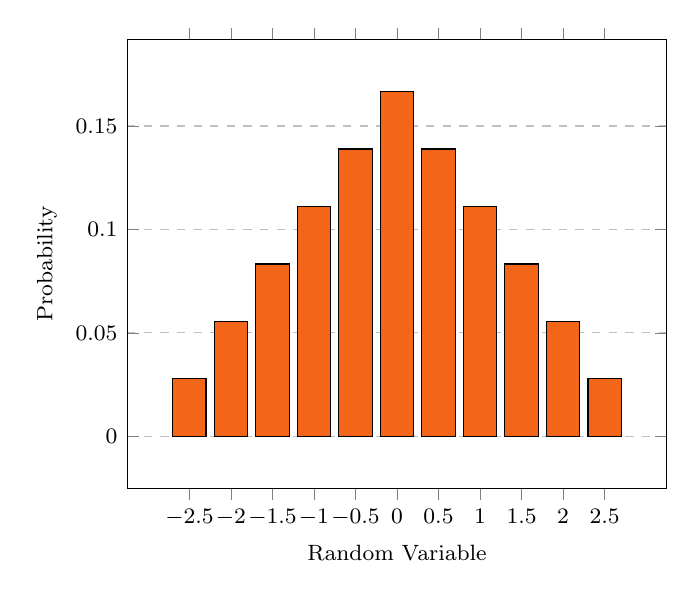
\begin{tikzpicture}
    \begin{axis}[
        ybar,
        bar width=12pt,
        ymin=0,
        xlabel={Random Variable},
        ylabel={Probability},
        xtick={-2.5,-2,...,2.5},
        xticklabel style={font=\footnotesize},
        yticklabel style={font=\footnotesize, /pgf/number format/fixed},
        xlabel style={font=\footnotesize},
        ylabel style={font=\footnotesize},
        xticklabel style={/pgf/number format/fixed},
        enlargelimits=0.15,
        ymajorgrids=true,
        grid style=dashed
    ]
    \addplot[fill={rgb,255:red,243;green,102;blue,25}] coordinates {
        (-2.5, 0.0278)
        (-2.0, 0.0556)
        (-1.5, 0.0833)
        (-1.0, 0.1111)
        (-0.5, 0.1389)
        (0.0, 0.1667)
        (0.5, 0.1389)
        (1.0, 0.1111)
        (1.5, 0.0833)
        (2.0, 0.0556)
        (2.5, 0.0278)
    };
    \end{axis}
\end{tikzpicture}
\caption{\label{fig:law_large_numbers_1}Probability mass function of the random variable $\frac{X_1 + X_2 }{2} - \mathbb{E}(X)$.}
\end{figure}

Now let's consider a random sample of size ten. In Figure \ref{fig:law_large_numbers_2} is depicted the probability mass function of the random variable $\frac{X_1 + X_2 + \ldots +  X_{10}}{10} - E(X): \Omega \times \ldots \times \Omega \rightarrow \mathbb{R}$. The probability $P(  |\frac{X_1 + X_2 + \ldots +  X_{10}}{10} - E(X)| < 1 )$ is $0.973$.

\begin{figure}[t]
\centering
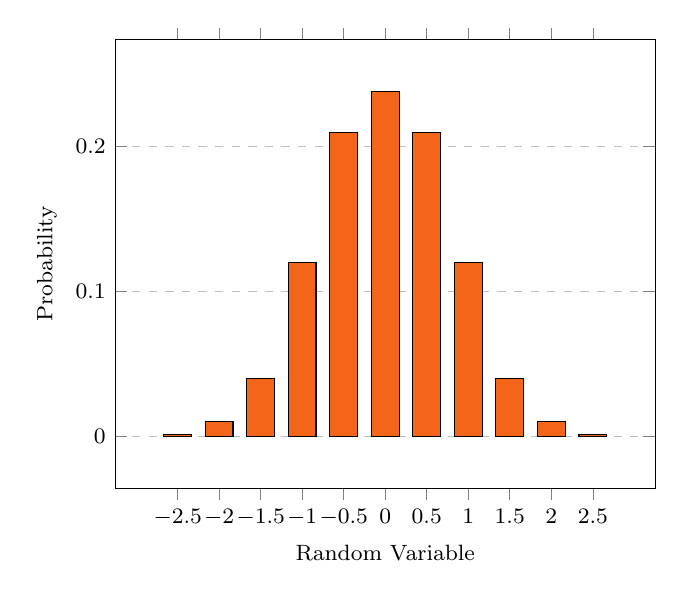
\begin{tikzpicture}
    \begin{axis}[
        ybar,
        bar width=10pt,
        ymin=0,
        xlabel={Random Variable},
        ylabel={Probability},
        xtick={-2.5,-2,-1.5,-1,-0.5,0,0.5,1,1.5,2,2.5},
        xticklabel style={font=\footnotesize},
        yticklabel style={font=\footnotesize},
        xlabel style={font=\footnotesize},
        ylabel style={font=\footnotesize},
        xticklabel style={/pgf/number format/fixed},
        enlargelimits=0.15,
        ymajorgrids=true,
        grid style=dashed
    ]
    \addplot[fill={rgb,255:red,243;green,102;blue,25}] coordinates {
        (-2.5, 0.0010)
        (-2.0, 0.0100)
        (-1.5, 0.0400)
        (-1.0, 0.1200)
        (-0.5, 0.2100)
        (0.0, 0.2380)
        (0.5, 0.2100)
        (1.0, 0.1200)
        (1.5, 0.0400)
        (2.0, 0.0100)
        (2.5, 0.0010)
    };
    \end{axis}
\end{tikzpicture}
\caption{\label{fig:law_large_numbers_2}Probability mass function of the random variable $\frac{X_1 + X_2 + \ldots +  X_{10}}{10} - E(X)$.}
\end{figure}

\end{example}

It is important to clarify that the law of large numbers refers to the sample mean, that is $\frac {1}{n} \sum_{i=1}^{n} X_{i}$, and it is not necesarily true for other formulas, like for example, the deviation from the theoretical expected value $\sum_{i=1}^{n} X_{i} - n \times E(X)$ which not only it does not converge, but inscreases in absolute value as $n$ increases (see Example \ref{ex:gambler's_fallacy}).

\begin{example}
\label{ex:gambler's_fallacy}
If we toss a fair coin, the probability that the outcome will be head is equal to $1/2$. According to the law of large numbers, the proportion of heads in a large number of coin tosses will be close to $1/2$. However, the difference between the number of heads and tails will not be close to zero. In fact, the larger the number of coin tosses, the larger will be this difference. This is a highly conterintuitive fact, since most of the people think that the more we toss the coin, the closer will be the number of heads to the number of tails, which is not true.
\end{example}

% Central Limit Theorem

\subsection{Central Limit Theorem}

Let $X_1, \ldots, X_n$ be a sample of $n$ independent and identically distributed random variables with mean $\mu$ and variance $\sigma^2$. As we saw in the previous section, the law of large numbers states that the sample average $\overline {X}_n$ converges in probability to $\mu$ as $n$ increases. The central limit theorem states that the distribution of the difference between the sample average $\overline {X}_n$ and the population mean $\mu$, when multiplied by the factor $\sqrt {n}$ approximates to the normal distribution with mean $0$ and variance $\sigma^2 / n$. The theorem is true regardless of the shape of the original random vairables.

\begin{theorem}[Central Limit Theorem]
\label{th:central_limit_theorem_pdf}\index{Central limit theorem}
Let $X_{1}, \ldots, X_{n}$ be a random sample of size $n$ from a distribution with mean $\mu$ and finite variance $\sigma^{2}$. Define the standardized sum as
\[
Z_n = \frac{\overline{X}_{n}-\mu}{\sigma/\sqrt{n}},
\]
where $\overline{X}_{n} = \frac{1}{n} \sum_{i=1}^{n} X_i$ is the sample mean. Then, as $n \rightarrow \infty$, the probability density function of $Z_n$ converges to the probability density function of the standard normal distribution $\phi(x)$, that is,
\[
\lim_{n \rightarrow \infty} f_{Z_n}(x) = \phi(x),
\]
where $f_{Z_n}(x)$ is the probability density function of $Z_n$, and $\phi(x)$ is the probability density function of the standard normal distribution, given by
\[
\phi(x) = \frac{1}{\sqrt{2\pi}} \exp\left(-\frac{x^2}{2}\right).
\]
\end{theorem}
\begin{proof}
Let $X_{1}, \ldots, X_{n}$ be independent and identically distributed (i.i.d.) random variables with mean $\mu$ and finite variance $\sigma^2$. Define the sample mean as
\[
\overline{X}_n = \frac{1}{n} \sum_{i=1}^{n} X_i.
\]
We are interested in the distribution of the standardized variable
\[
Z_n = \frac{\overline{X}_n - \mu}{\sigma / \sqrt{n}}.
\]

First, consider the sum of the $X_i$'s, which we write as
\[
S_n = \sum_{i=1}^{n} X_i.
\]
The sample mean can then be written as
\[
\overline{X}_n = \frac{S_n}{n}.
\]
Thus, the standardized variable $Z_n$ becomes
\[
Z_n = \frac{S_n - n\mu}{\sigma\sqrt{n}}.
\]

To analyze the behavior of $Z_n$ as $n \to \infty$, we consider the sum $S_n = \sum_{i=1}^{n} X_i$. According to the Law of Large Numbers, $S_n/n$ converges to $\mu$, and hence $Z_n$ should converge to a normal distribution due to the nature of sums of independent random variables.

For large $n$, $Z_n$ can be approximated by considering the Taylor expansion of the exponential function. Since the $X_i$'s are i.i.d., the distribution of $S_n$ can be approximated by a normal distribution with mean $n\mu$ and variance $n\sigma^2$. The key idea is that as $n$ increases, the distribution of $Z_n$ approaches a normal distribution because the sum of i.i.d. random variables tends to be normally distributed by the Central Limit Theorem.

Let us consider the moment generating function (MGF) of $Z_n$. The MGF of $Z_n$ is given by:
\[
M_{Z_n}(t) = \mathbb{E}\left[\exp\left(t Z_n\right)\right] = \mathbb{E}\left[\exp\left(t \frac{S_n - n\mu}{\sigma\sqrt{n}}\right)\right].
\]
For large $n$, by the Central Limit Theorem, the MGF of $Z_n$ approaches that of a standard normal variable $N(0,1)$:
\[
M_{Z_n}(t) \approx \exp\left(\frac{t^2}{2}\right),
\]
which implies that $Z_n$ converges in distribution to $N(0,1)$ as $n \to \infty$.

Since $Z_n$ converges in distribution to $N(0,1)$, the probability density function of $Z_n$, denoted by $f_{Z_n}(x)$, must converge to the probability density function of a standard normal distribution $\phi(x)$, given by:
\[
\phi(x) = \frac{1}{\sqrt{2\pi}} \exp\left(-\frac{x^2}{2}\right).
\]
Thus, we have
\[
\lim_{n \rightarrow \infty} f_{Z_n}(x) = \phi(x).
\]

Therefore, as $n \to \infty$, the distribution of the standardized sum $Z_n$ approaches the standard normal distribution, completing the proof.
\end{proof}

The Central Limit Theorem is a fundamental concept in probability theory used in statistical analysis and inference. It allows us to compute the probability that the sample average is close to the distribution mean. It is important to recall the conditons for the central limit theorem to be true: the samples must be independent and identically distributed, the original distribution has to have a finite variance, and the sample size must be sufficiently large.

\begin{example}
Suppose a factory produces light bulbs, and the lifespan of each light bulb is a random variable with a mean of $\mu = 1000$ hours and a standard deviation of $\sigma = 50$ hours. The factory tests a random sample of $n = 36$ light bulbs to estimate the average lifespan of the bulbs produced in a particular batch. What is the probability that the sample mean lifespan of these 36 bulbs is between 990 and 1010 hours?

We can apply the Central Limit Theorem to solve this problem because we are dealing with the sample mean of a large number of independent, identically distributed random variables (lifespans of light bulbs). First, define the sample mean $\overline{X}_n$ as:
\[
\overline{X}_n = \frac{1}{n} \sum_{i=1}^{n} X_i,
\]
where $X_i$ represents the lifespan of the $i$-th light bulb in the sample, and $n = 36$ is the sample size.

By the Central Limit Theorem, for sufficiently large $n$, the distribution of the sample mean $\overline{X}_n$ approaches a normal distribution with mean $\mu$ and standard deviation $\sigma/\sqrt{n}$:
\[
\overline{X}_n \sim N\left(\mu, \frac{\sigma}{\sqrt{n}}\right) = N\left(1000, \frac{50}{\sqrt{36}}\right) = N\left(1000, \frac{50}{6}\right) = N\left(1000, 8.33\right).
\]

Next, we calculate the z-scores corresponding to 990 hours and 1010 hours using the formula:
\[
z = \frac{X - \mu}{\sigma/\sqrt{n}},
\]
where $X$ is the value for which we want to find the z-score.

For $X = 990$:
\[
z_{990} = \frac{990 - 1000}{8.33} \approx \frac{-10}{8.33} \approx -1.20.
\]

For $X = 1010$:
\[
z_{1010} = \frac{1010 - 1000}{8.33} \approx \frac{10}{8.33} \approx 1.20.
\]

Now, we use the standard normal distribution table (or a calculator) to find the probabilities corresponding to these z-scores:
\[
P(z_{990} \leq Z \leq z_{1010}) = P(-1.20 \leq Z \leq 1.20).
\]

From the standard normal distribution table:
\[
P(Z \leq 1.20) \approx 0.8849,
\]
\[
P(Z \leq -1.20) \approx 0.1151.
\]

Thus, the probability that the sample mean lifespan of the 36 light bulbs is between 990 and 1010 hours is:
\[
P(990 \leq \overline{X}_n \leq 1010) = P(-1.20 \leq Z \leq 1.20) = 0.8849 - 0.1151 = 0.7698.
\]

The probability that the sample mean lifespan of the 36 light bulbs falls between 990 and 1010 hours is approximately 76.98\%. This result demonstrates how the Central Limit Theorem allows us to use the normal distribution to approximate the sampling distribution of the sample mean, even when the original data is not normally distributed, as long as the sample size is sufficiently large.
\end{example}

%
% Section: References
%
\section*{References}

\cite{degroot1986probability} is a widely respected textbook in the fields of statistics and probability theory. First published in 1975, this book is known for its clear exposition of the fundamental concepts of probability and statistics, making it suitable for both beginners and those with some background in the subject. The book's approach balances theory and application, making it useful both for learning theoretical underpinnings and for applying probability and statistics to real-world problems.

\cite{childers2013philosophy} offers a comprehensive introduction to the foundational aspects of probability, with a focus on the philosophical questions it raises. Childers explores various interpretations of probability, including frequentist, propensity, classical, Bayesian, and objective Bayesian, and presents these complex ideas in a way that is accessible even to those without a strong background in probability or mathematics.

An example of the problems associated with the misinterpretation of expected value is the St. Petersburg Paradox\index{St. Petersburg Paradox}. Introduced by Nicholas Bernoulli in 1713, this paradox involves a gambling game with an infinite expected payoff, yet no reasonable person would pay more than \$25 to play it. Despite being three centuries old, the paradox continues to inspire new arguments and solutions in recent years (see \cite{huang2013three} for a historical review of the main proposed solutions).


%
% CHAPTER: Computability
%

%
% CHAPTER.- Computability
%

\chapterimage{TuringMachine.pdf}

\chapter{Computability}
\label{chap:Computability}

\begin{quote}
\begin{flushright}
\emph{Caminante, no hay camino,\\
se hace camino al andar.\footnote{Wanderer, there is no road, the road is made by walking.}}\\
Antonio Machado
\end{flushright}
\end{quote}
\bigskip

We begin our review of the background required to understand the theory of nescience by providing a mathematical formalization of the concept of a \emph{computable procedure}\index{Computable procedure}. Intuitively, a computable procedure is a method consisting of a finite number of instructions that, when applied to a problem, produce the correct answer after a finite number of steps. The key point is that the instructions must be clear and precise enough for any human to follow without aid. We can even go a step further and requre that the instructions must be so straightforward that a machine could execute them. In 1936, British mathematician Alan Turing introduced a formal model for a family of hypothetical machines and posited that for every computable procedure (in its intuitive sense), there exists a \emph{Turing machine}\index{Turing machine} capable of computing it. The model was not only simple enough for precise mathematical analysis but also versatile and powerful.

Over the years, many alternative proposals have aimed to formalize the concept of computable procedure. Some have been very complicated, but all have proven equivalent to the concept of the Turing machine; that is, they solve the same set of problems. Two notable examples of alternative definitions are the \emph{lambda calculus}\index{Lambda calculus} by Alonzo Church and the \emph{theory of recursive functions}\index{Recursive function} by Kurt Gödel and Stephen Kleene. The \emph{Church-Turing thesis}\index{Church-Turing thesis} asserts that any formalization of the concept of a computable procedure, meeting some minimum requirements (such as performing a finite amount of work in a single step), is equivalent to a Turing machine. This thesis suggests an objective notion of a computable procedure that is independent of any specific formalization.

The concept of the Turing machine, initially referring to mechanical devices designed to solve individual problems, has been extended and universalized. A \emph{universal Turing machine}\index{Universal Turing machine} exists that can resolve all computable problems by simulating the behavior of other specific machines, akin to how modern computers run algorithms written in various programming languages. This concept raises a significant question: Are there problems that are not computable? We will see that the answer is affirmative, certain well-defined problems exceed the computational capabilities of computers, and such problems are more common than initially anticipated. The notion of uncomputable functions will be pivotal in our theory of nescience.

Given the abstract nature of most entities studied in science, we employ the concept of the \emph{oracle Turing machine}\index{Oracle Turing machine} to aptly formalize our theory. An oracle Turing machine resembles a regular Turing machine but is augmented with the capability to query an external oracle, whose workings are not fully understood, to aid in its computations. This oracle can address problems that are unresolvable by standard Turing machines—essentially, it can solve uncomputable problems. The oracle is a theoretical construct that represents a source of solutions or information that is not bound by the limitations of computability. It acts as a ‘black box’ that instantly provides answers to specific questions or problems, enabling the oracle Turing machine to transcend its computational boundaries. The oracle is an abstract and non-mechanical entity, a theoretical tool used to explore the bounds of computation, rather than a physical or concrete machine that can be built or observed.

Turing machines illuminate the inherent limitations of our computational capabilities. This exploration into the abstract and theoretical realms of computation is not just a philosophical endeavor; it also possesses practical applications in the field of \emph{computational complexity}\index{Computational complexity}. Located at the intersection of computer science and mathematics, computational complexity evaluates the challenges associated with solving problems, measured against the required resources, notably time and space. Problems are classified based on their intrinsic complexity and the computational effort required for their resolution. One of the key questions in this field is the elusive and yet unsolved $P\overset{?}{=}NP$\index{$P\overset{?}{=}NP$} question, which seeks to determine if the class $P$ of problems, those that are easy to solve, coincides with the class $NP$ of problems, whose solutions are easy to verify. In this book, our focus is not solely on the epistemological question of identifying which problems can be effectively solved given ample time and space, but also on those that can be resolved efficiently in time.

%
% Section: Turing Machines
%

\section{Turing Machines}\index{Turing Machine}
\label{sec:Turing-Machines}

A Turing machine is a extremely simplified model of a general purpose computer, but capable of solving any problem that real computers can solve. From an intuitive point of view, we could see the machine as composed of a head that operates on a two-way infinite striped tape of symbols; at every time step the machine reads the symbol under the head and decides whether to write a new symbol on the tape, move the head one square (left or right), or do both things; algorithms are implemented using an internal table of rules in the control head, and the actual input to the algorithm is codified on the tape; when the machine reaches the final state, the algorithm's output is on the tape. Figure \ref{fig:Turing-Machine} depicts an example of a machine in its initial state with the head located at the beginning of the input string.

\begin{figure}[h]
\centering\includegraphics[scale=0.5]{TM}
\caption{\label{fig:Turing-Machine}Turing Machine}
\end{figure}

\begin{definition}[Turing Machine]
\label{def:Turing-Machine}
A \emph{Turing machine} is a 7-tuple $\left(Q,\Gamma,\sqcup,\Sigma,q_{i},q_{f},\tau\right)$ where:
\begin{align*}
 & Q \quad \text{is a finite, non-empty, set of \emph{states},} \index{Machine State} \\
 & \Gamma \quad \text{is a finite, non-empty, set of \emph{tape symbols},} \index{Tape Symbol} \\
 & \sqcup\in\Gamma \quad \text{is the \emph{blank symbol},} \index{Blank Symbol} \\
 & \Sigma\subseteq\Gamma\setminus\sqcup \quad \text{is the set of \emph{input symbols},}  \index{Input Symbol} \\
 & q_{o}\in Q \quad \text{is the \emph{initial state},} \index{Initial State} \\
 & q_{f}\in Q \setminus \{q_o\} \quad \text{is the \emph{final state},} \index{Final State} \\ 
 & \tau:\left(Q\setminus \{q_{f}\}\right)\times\Gamma \rightarrow  Q\times\Gamma\times\left\{ L,R,S\right\} \quad\text{is a partial \emph{transition function}. \index{Transition Function} }
\end{align*}
\end{definition}

The algorithm implemented by the machine is given by the transition function $\tau$. This function specifies that given the current state of the machine and the tape symbol under the head, the machine will reach a new state, will write a new symbol on tape (or leave the old symbol unchanged), and will move the head to the left, to the right, or stay in place ($L$, $R$ or $S$ respectively). After a finite, uniquely determined, succession of steps, the machine will reach the final state $q_f$ and \emph{halts} (the machine does not make any further move after halting). The output of the algorithm is the unique string of symbols $s \in \Sigma^\ast$  that is left on the tape after halting. Eventually, some machines could iterate forever, never halting. If an undefined transition is reached, the machine will get stalled.

The input to the machine is a string of symbols, and we assume that in the initial state the head of the machine is located at the first symbol of the input string. If we want to solve a problem related to an object $O$ other than a string, fist we have to provide a method to encode that object using a string $\left\langle O \right\rangle$.

\begin{example}
\label{ex:Turing-Machine}
The following Turing machine solves the problem of adding two natural numbers: the set of states is $Q = \left\{q_{o}, q_{1}, q_{f}\right\}$, the set of tape symbols is $\Gamma = \left\{0, 1, \sqcup \right\}$, the set of input symbols is $\mathcal{B} = \left\{0, 1 \right\}$, and the transition function is given by the following table (rows are indexed by machine states, and columns by tape symbols):

\begin{table}[h]
\centering
\begin{tabular}{l l l l}
\toprule
 & 0 & 1 & $\sqcup$ \\
\midrule
$q_{o}$ & $\left(q_{f}, \sqcup, S\right)$ & $\left(q_{1}, \sqcup, R\right)$ & $\uparrow$ \\
$q_{1}$ & $\left(q_{f}, 1     , S\right)$ & $\left(q_{f}, 1     , R\right)$ & $\uparrow$ \\
\bottomrule
\end{tabular}
\caption{Transition Rules}
\end{table}

Given the natural numbers $n$ and $m$, the input string for this machine is $n$ 1's followed by a $0$ and followed by $m$ 1's. The output is a string of $n+m$ consecutive 1's. For example, if we want to add the numbers 2 and 3 the input string should be $\sqcup 1 1 0 1 1 1 \sqcup$, and the machine output string would be $\sqcup 1 1 1 1 1 \sqcup$.
\end{example}

A Turing machine can be also represented by a \emph{state diagram}\index{State diagram}. A state diagram is similar to a labeled directed graph\footnote{In this particular case we allow loops and multiple edges coming out from vertices.} where the vertices are the states of the machine, the edges represent a movement from one state to another state, and the edge labels shows the symbol under the head that yields to the new state, together with the symbol written down in the tape and the movement of the head. Under these conventions, the state diagram of the Turing machine of Example \ref{ex:Turing-Machine} is depicted in Figure \ref{fig:Example-Turing-Machine}.

\begin{figure}[h]
\centering\includegraphics[scale=0.5]{ETM}
\caption{\label{fig:Example-Turing-Machine}Example of Turing Machine}
\end{figure}

It is a remarkable fact that small changes to the actual definition of Turing machine do not alter its power. That is, it is a highly robust definition. In Example \ref{ex:multitape_turing_machine} it is shown that adding more tapes to the machines does not increase the number of problems that can be solved using this model. Similar proofs can be provided for the case of adding a finite storage to the control tape, allowing parallel processing with multiple control heads, and so on.

\begin{example}
\label{ex:multitape_turing_machine}
A \emph{multitape Turing machine}\index{Multitape Turing machine} is a Turing machine that has multiple heads with their corresponding tapes. At the starting configuration the input string is in tape 1 and all the others tapes are blank. The transition function of a multitape Turing machine is:
\[
\tau:\left(Q \setminus q_{f} \right) \times \Gamma^k \rightarrow  Q \times \Gamma^k \times \left\{L,R,S\right\}^k.
\]
where $k$ is the number of tapes. Multitape Turing machines are equivalent to regular Turing machines. We can prove this assertion by providing a mechanism in which a regular Turing machine can simulate the behavior of a multitape machine. In order to do that we have to encode the content of the multiple tapes into a single tape, introducing a new symbol that will act as tape separator, and to codify the location of the heads in all those tapes, by means of a new head location symbol. If the tape separation symbol is $|$ and the head location symbol is $h$, a simulation tape of a 3-tapes machine could looks something like $\sqcup01h00|000h1|h0101\sqcup$. The operation of the regular machine just scans one by one the subtapes locating the head position and performing the required transition. If the computation of one subtape requires to write a new symbol beyond it limits, we have to shift the rest of the symbols to make room to the new symbol. Of course, the operation of the simulation will be much slower than the original multitape machine, but the set of problems that can be solved with the two types of machines is exactly the same.
\end{example}

Without any loss of generality, for the rest of this book we will assume that the set of input symbols $\Sigma = \mathcal{B}$ and that the set of tape symbols $\Gamma = \left\{0, 1, \sqcup \right\}$.

\begin{definition}\index{Configuration}
A \emph{configuration} of a Turing machine $T$ is the 3-tuple $\left(q,s,i\right)$, where $q\in Q$ is an state of the machine, $s\in\Gamma^+$ is a string with the contents of the tape (excluding the blank symbols), and $1 \le i \le n$ is the index of the symbol $s_i$ under the head, where $s_1$ is the first non-blank symbol of the tape and $n=l(s)$. 
\end{definition}

Configurations allow us to losslessly describe the current state of a Turing machine. At any step of a computation we could stop the machine, write down its current configuration, and later on continue the computation at the same point where we left, just by reading its configuration.

\begin{definition}\index{Configuration yields configuration}
We say that configuration $C=\left(q,s,i\right)$ \emph{yields} configuration $C'=\left(r,s',j\right)$ if there exists a transition $\tau:\left(q, s_{i}\right) = \left(r, s'_{i}, a\right)$, where $s=s_{1} \dots s_{i-1}s_{i}s_{i+1} \dots s_{n}$, $s'=s_{1} \dots s_{i-1}s'_{i}s_{i+1} \dots s_{n}$, and
\begin{equation}
  j = \begin{cases}
        i+1 & \text{if $a=R$} \\
        i-1 & \text{if $a=L$} \\
        i   & \text{if $a=S$}
  \end{cases}
\end{equation}
\end{definition}

Given the concepts of configuration and configuration that yields a new configuration we can formally define what we mean by computation.

\begin{definition}[Computation]\index{Computation}
Let $T$ be a Turing machine, $C_{0}$ the starting configuration of the machine, and $C_n$ a configuration containing the final state $q_f$. A \emph{computation} under machine $T$ is a finite sequence of $n+1$ configurations $\left(C_{0},C_{1},\ldots,C_n\right)$ in which each configuration $C_{k}$ yields the configuration $C_{k+1}$, for all $0\leq k < n$.
\end{definition}

Computations are deterministic, that is, given a Turing machine $T$ and an input string $s$, the sequence of configurations is predetermined. If the machine $T$ does not halt, or it get stalled, on input $s$, we say that there was no computation.

\begin{example}
The computation of the Turing machine described in Example \ref{ex:Turing-Machine} with the input string $110111$ is the following sequence of configurations:

\begin{enumerate}
\item $(q_0, 110111, 1)$
\item $(q_1, 10111,  1)$
\item $(q_1, 10111,  2)$  
\item $(q_f, 11111,  2)$  
\end{enumerate}

\end{example}

The next theorem states that our intuitive notion of computable procedure is equivalent to the concept of Turing machine. This result is not a regular theorem, since it cannot be formally proved. Some authors call it \emph{thesis} instead of theorem; Turing himself called it a \emph{definition}.

\begin{theorem}[Turing's Thesis]
\label{th:turing_thesis}
A procedure can be computed by a human being if, and only if, it can be computed by a Turing machine.
\end{theorem}

As we have mentioned in the introduction of this chapter, all the other alternative formalizations of the concept of computable procedure proposed so far are equivalent in expressive power to Turing machines. 

%
% Section: Universal Turing Machine
%

\section{Universal Turing Machines}
\label{sec:Universal-Turing-Machines}

In Section \ref{sec:Turing-Machines} we saw how to store the current state of a Turing machine so that the computation could be stopped and later on resumed. In Example \ref{ex:Encoding_TM} we are going to see a similar procedure, not to store the current state of the machine, but to save a full description of the machine itself. This procedure will allow us to enumerate, that is, to list all possible Turing machines. This enumeration will enable us to prove that there exists problems that are not solved by any Turing machine (see Section \ref{sec:non_computable_problems}), and to introduce the very important concept of \emph{Universal Turing Machine}.

\begin{example}
\label{ex:Encoding_TM}
In order to loosely describe a Turing machine we have to encode the transition function $\tau:\left(Q\setminus \{q_{f}\}\right)\times\Gamma\rightarrow Q\times\Gamma\times\left\{ L,R,S\right\}$. This function can be represented as a collection of quintuples $\left(q,s,r,t,a\right)$ where $q \in \left(Q\setminus \{q_{f}\}\right)$, $r \in Q$, $s$ and $t\in\Gamma$, and $a\in\left\{ L,R,S\right\}$. In this way, any Turing machine $T$ will be fully described by a collection of quintuples:
\[
\left(q_{1},s_{1},r_{1},t_{1},a_{1}\right),\left(q_{2},s_{2},r_{2},t_{2},a_{2}\right),\ldots,\left(q_{m},s_
{m},r_{m},t_{m},a_{m}\right)
\]
where $m \leq d\left(Q\setminus \{q_{f}\} \times d(\Gamma) \right)$, with the additional requirement that the first quintuple should refer to the initial state, and second one to the final state, that is $q_{1} = q_{o}$ and $r_{2} = q_{f}$. A possible description of these quituples would be to encode the elements of the set $Q\cup\Gamma\cup\left\{ L, R, S \right\}$ using a fixed length binary code (see Definition \ref{def:Fixed-Length-Codes} for more information about these codes), so the quintuple $\left(q,s,r,t,a\right)$ would be encoded as $\left\langle q, s, r, t, a \right\rangle$. The length of an encoded quintuple is $5l$, where $l=\left\lceil \log\left(d\left(Q\cup\Gamma\cup\left\{ L,R,S\right\} \right)\right)\right\rceil$. Using those conventions, the machine $T$ would be encoded as the binary string:
\[
\left\langle T \right\rangle = \left\langle \bar{l}, \left\langle q_{1}, r_{1}, s_{1}, t_{1}, a_{1} \right\rangle, \ldots, \left\langle q_{r}, r_{r}, s_{r}, t_{r}, a_{r} \right\rangle \right\rangle 
\]
The length of the encoded machine using this schema would be $l(\left\langle T \right\rangle) \leq 5lm + \log l + 1$.
\end{example}

Since each Turing machine is composed by a finite set of quintuples, we can encode and list all the machines using a shortlex ordering. We associate each machine $T$ with the index $i$ corresponding to its position in this list, and we denote by $T_i$ the i-th Turing machine. Each positive integer $i$ encodes one, and only one, Turing machine. However, as Proposition \ref{prop:padding_lemman} shows, all Turing machines have an infinite number of indexes. We associate each Turing machine with its smallest index.

\begin{proposition}[Padding Lemma]
\label{prop:padding_lemman}
Each Turing machine has infinitely many indexes.
\end{proposition}
\begin{proof}
If $T_i$ is the i-th Turing machine encoded by the string $\langle T_i \rangle$, we can add an finite number of 0's to the end of this string, resulting in a new encoding index $j$, that encodes the same machine.
\end{proof}

A universal Turing machine is a machine that can simulate the behavior of any other Turing machine on arbitrary input. The universal machine essentially achieves this by reading from its own tape both the description of the machine to be simulated (for instance, using the coding schema described in Example \ref{ex:Encoding_TM}), as well as the input string to be used during the computation.

\begin{definition}[Universal Turing Machine]
\label{def:Universal-Turing-Machine}
\index{Universal Turing machine}
A \emph{Universal Turing Machine} is a Turing machine $U$ such that $U(\langle \langle T_i\rangle, s \rangle) = T_i(s)$ for all Turing machines $T_i$ and all input strings $s \in \mathcal{B}$.
\end{definition}

Of course, we have to prove that such machine exits before we can use it. We could argue that a human being would be able to decode the machine $T_i$ and simulate its behavior with the input string $s$, and then refer to Theorem \ref{th:turing_thesis}. A better approach would be to explicitly build an universal Turing machine. However, describing one of these machines is out of the scope of this book. Instead, we refer to the reader to the references included at the end of the chapter.

%
% Section: Non computable problems
%

\section{Non-Computable Problems}
\label{sec:non_computable_problems}

Turing machines allow us to identify which problems can be solved using effective procedures, that is, the set of problems that can be worked out with computers. Although it might be a bit surprising, there exists many problems that cannot be solved using algorithms. These problems are beyond the capabilities of computers. We are not talking about problems like if a computer can be intelligent or if it can be self-aware, we refer to well defined mathematical problems. For example, the famous \emph{halting problem} asks to find a computer program that, given any other program and an input string, decides if the program will eventually stop for that input string, or if it will keep running forever.

\begin{algorithm}
\caption{HALT function}
\label{alg:halt}
\begin{algorithmic}
\Procedure{HALT}{$A, I$}
    \If{$A(I)$ halts} 
        \State \textbf{return} $1$
    \Else
        \State \textbf{return} $0$
    \EndIf
\EndProcedure
\end{algorithmic}
\end{algorithm}

\begin{theorem}[Halting Problem]
\index{Halting problem}
\label{th:halting-problem}
Define the HALT as in Algorithm \ref{alg:halt}. It does not exists a Turing machine that computes the $HALT$ function for all possible pairs $(A, I)$, where $A$ is a Turing machine and $I$ is the input string to that machine.
\end{theorem}
\begin{proof}
The proof is by contradiction. Assume that the machine $HALT$  exists, and define a new Turing machine $TC$ such that $TC(A) = 1$ if $HALT(A,A) = 0$, and $TC(A)$ will never stop if $HALT(A,A) = 1$. Then the contradiction arises when we ask about the result of $TC(TC)$: if $TC(TC)$ stops we have that $HALT(TC,TC) = 0$ and that $TC(TC)$ should not stop, and if $TC(TC)$ does not stop then we have that $H(TC,TC) = 1$ and thus $TC(TC)$ should stop.
\end{proof}

A very important consequence of the Halting Problem is that there exists more well-defined mathematical problems than computable solutions\footnote{It is still an open question if there exists non-computable problems in Nature.}. The Halting Problem has also important practical consequences in computer programming. For example, we cannot write a program that can guarantee that any other arbitrary program is bug-free, or that all infinite loops with conditional exits will eventually stop for all possible inputs.

Incomputability is not only about halting. Next example shows a well defined practical problem involving simple strings manipulation that can not be solved using computers.

\begin{example}
\label{ex:PCP}
Given two finite lists $\left( \alpha_1, \ldots, \alpha_n \right)$ and $\left( \beta_1, \ldots, \beta_n \right)$ of strings over some alphabet $\Sigma$, where $d(\Sigma) \ge 2$, the \emph{Post Correspondence Problem}, or PCP, asks to decide if there exists a sequence of $K \geq 1$ indices $(i_k)$, where $1 \le i_k \le n$ for all $1 \le k \le K$, such that $\alpha_{i_1} \ldots \alpha_{i_K} = \beta_{i_1} \ldots \beta_{i_K}$. For example, given the sequences $(a, ab, bba)$ and $(baa, aa, bb)$, a solution to the problem would be $\alpha_3 \alpha_2 \alpha_3 \alpha_1 = \beta_{3} \beta_{2} \beta_{3} \beta_{1}$. It does not exist an algorithm to solve PCP. As many proofs of incomputability, the proof proceed by showing that HALT can be reduced to PCP, that is, if PCP is decidable then the Halting problem should be decidable as well. We are not going to show the details of the proof in this section. For the interested reader, we refer to the references at the end of this chapter.
\end{example}

%
% Section: Computable Functions and Sets
%

\section{Computable Functions and Sets}
\label{sec:computable_functions}

Each Turing machine $T$ defines a function $f_T:\mathcal{B}^{\ast}\rightarrow\mathcal{B}^{\ast}$ that for each input string $s\in\mathcal{B}^{\ast}$ assigns the output string $T(s)\in\mathcal{B}^{\ast}$. This relation between Turing machines and functions allows us to introduce the concept of \emph{computable function}. 

\begin{definition}
\label{def:computable-function}
\index{Computable Function}
A function $f:\mathcal{B}^{\ast}\rightarrow\mathcal{B}^{\ast}$ is \emph{computable} is there exist a Turing machine $T$ such that it defines the function $f$.
\end{definition}

Computable functions are also called \emph{recursive functions}. However, since we are not going to cover the theory of recursive functions in this book, we prefer the term computable functions.

\begin{example}
The function that assigns to each pair of natural numbers $x$ and $y$ its sum $x + y$ is a computable function, as it is shown in Example \ref{ex:Turing-Machine}. In this particular case, we have transformed the original function $f: \mathbb{N} \times \mathbb{N} \rightarrow \mathbb{N}$ into a new function $g:\mathcal{B}^{\ast}\rightarrow\mathcal{B}^{\ast}$ by means of encoding natural numbers as strings of 1's, and the pair of numbers $x$, $y$ into a single string $\left\langle x, y \right\rangle$.
\end{example}

Partial functions can be defined by Turing machines that do not halt on the undefined values of the function.

\begin{definition}
A partial function $f:\mathcal{B}^{\ast}\rightarrow\mathcal{B}^{\ast}$ is \emph{partial computable} is there exist a Turing machine $T$ such that it defines the function $f$ for those values in which $f$ is defined, and $T$ does not halt for those values in which $f$ is not defined.
\end{definition}

\begin{example}
The function $f: \mathbb{N} \times \mathbb{N} \rightarrow \mathbb{N}$ that assigns to each pair of natural numbers $x$ and $y$ the number $x - y$ is a partial computable function, since it is not defined in the case that $x < y$.
\end{example}

We can apply the same concepts of computable and partial computable to sets.

\begin{definition}
A set $A \in \mathcal{B}^\ast$ is \emph{computable} if its characteristic function $\mathcal{X}_A$ is a total computable function. A set $A \in \mathcal{B}^\ast$ is \emph{computably enumerable} if its characteristic function $\mathcal{X}_A$ is a partial computable function, that is, $\mathcal{X}_A(a) = 1$ if $a \in A$, but $\mathcal{X}_A(a)$ is undefined if $a \not\in A$.
\end{definition}

\begin{example}
The set of all Turing machines that halt on all inputs is not computable, as we have shown in Theorem \ref{th:halting-problem}, although it is computably enumerable.
\end{example}

%
% Section: Oracle Turing Machine
%

\section{Oracle Turing Machine}
\label{sec:oracle_turing_machine}

{\color{red} TODO: Introduce the concept}

{\color{red} TODO: Provide a diagram}

Withe the aid of the Oracle, a Turing machine could solve uncomputable problems, like the halting problem.

{\color{red} The oracle tape is a one-way unbounded, read-only tape that contains all the values of the characteristic function $\chi_\mathcal{O}$. We assume that it takes, for arbitrary $w \in \Sigma^\ast$, only one step to search the tape and return the value of $\chi_\mathcal{O}(w)$.}

\begin{definition}[Oracle Turing Machine]
\label{def:Oracle-Turing-Machine}
An \emph{oracle Turing machine} with oracle set $\mathcal{O}$ is a 8-tuple $\left(Q, \Gamma, \sqcup, \Sigma, q_i, q_f, \tau, \mathcal{O} \right)$ where:
\begin{align*}
 & Q \quad \text{is a finite, non-empty, set of \emph{states},} \index{Machine State} \\
 & \Gamma \quad \text{is a finite, non-empty, set of \emph{tape symbols},} \index{Tape Symbol} \\
 & \sqcup\in\Gamma \quad \text{is the \emph{blank symbol},} \index{Blank Symbol} \\
 & \Sigma\subseteq\Gamma\setminus\sqcup \quad \text{is the set of \emph{input symbols},}  \index{Input Symbol} \\
 & q_{o}\in Q \quad \text{is the \emph{initial state},} \index{Initial State} \\
 & q_{f}\in Q \setminus \{q_o\} \quad \text{is the \emph{final state},} \index{Final State} \\ 
 & \tau: \left(Q \setminus \{q_{f}\}\right) \times \Gamma \times \{0, 1\} \rightarrow  Q\times\Gamma\times\left\{ L,R,S\right\} \quad\text{is the \emph{transition function}, \index{Transition Function} } \\
 & \mathcal{O} \subseteq \Sigma^\ast \quad \text{is the \emph{oracle set}.}
\end{align*}
\end{definition}

Properties:

 * The machine is independent of the oracle set
 * Turing machines are a subset of oracle Turing machines

Talk about:

 * How to encode oracle Turing machines
 * What means a function or set to be oracle computable
 * 

%
% Section: Computational Complexity
%

\section{Computational Complexity}
\label{sec:computational_complexity}

{\color{red} Computational Complexity theory is an investigation of the time, memory, or other resources required for solving computational problems.} In this book we are insterested mostly in the time required to solve a problem. {\color{red} We compute the running time of an algorithm as a function of the length of the string representing the input.}

{\color{red} TODO: Adapt this definiton.}
\begin{definition}
Let $M$ a deterministic Turing machine that halts on all inputs. The running time or time complexity of $M$ is the function $f:\mathbb{N}\rightarrow\mathbb{N}$, where $f(n)$ is the maximum number of steps that $M$ uses in any input of length $n$. If $f(n)$ is the running time of $M$, we say that $M$ runs in time $f(n)$ and that $M$ is an $f(n)$ time Turing machine.
\end{definition}

{\color{red} It considers only the highest order term of the expression for the running time of the algorithm, disregarding both the coefficient of that term and any lower order terms.}

{\color{red} Introduce polynomial bounds $O(n^c)$}

{\color{red} TODO: Adapt this definiton.}
Let $t:\mathbb{N}\rightarrow\mathbb{R}^{+}$ be a function. Define the time complexity class, $TIME(t(n))$, to be the collection of all languages that are decidible by an $O(t(n))$ time Turing machine.

{\color{red} TODO: Add the following as an example:
Let $t(n)$ be a function, where $t(n)\geq n$. Then every $t(n)$ time multiple tape Turing machine has an equivalent $O(t^{2}(n))$ time single-tape Turing machine.
}

{\color{red} Polynomial differences in running time are considered to be small, whereas exponential differeces are considered to be large.}


{\color{red} Adapt this definition:
\begin{definition}
$P$ is the class of languages that are decidible in polynomial time on a deterministic single-tape Turing machine $P=\cup_{k}TIME(n^{k})$.
\end{definition} 

$P$ roughly corresponds to the class of problems that are realistically solvable on a computer.}

{\color{red} Add the following example of problem in P: PATH = \{ $\langle G,s,t\rangle|G$ is a directed graph that has directed path from $s$ to $t$ }

{\color{red} Adapt this definition:
\begin{definition}
A verifier for a language $A$ is an algorithm $V$, where $A=\{w|V$ accepts $\langle w, c\rangle$ for some string $c\}$.
\end{definition}
}

{\color{red} We measure the time of a verier only in terms of the length of $w$, so a polynomial time verifier runs in polynomial time in the length of $w$
. A language $A$ is polynomially verifiable if it has a polynomial time verifier. The symbol $c$ is called a certificate, or proof of membership in $A$.}

{\color{red}
\begin{definition}
$NP$ is the class of languages that have polynomial time verifiers.
\end{definition}
}


{\color{red} TODO: Include an example.}

{\color{red} $P$ is the class of languages for which membership can be decided quickly. $NP$ is the class of languages for which membership can be verified quickly. The question of whether $P=NP$ is one of the greatest unsolved problems in theoretical computer science and contemporary mathematics.}


{\color{red} TODO: Not sure about the rest of this chapter:

Definition 14. A function $f:\Sigma^{\ast}\rightarrow\Sigma^{\ast}$ is a polynomial time computable function if some polynomial time Turing machine $M$ exists that halts with just $f(w)$ on its tape, when started on any imput $w$.

When problem $A$ reduces to problem $B$, a solution to $B$ can be used to solve $A$.

Definition 15. Language $A$ is polynomial time mapping reducible, or simply polynomial time reducible, to language $B$, written $A\leq_{P}B$, if a polynomial time computable function $f:\Sigma^{\ast}\rightarrow\Sigma^{\ast}$ exists, where for every $w$ $w\in A\iff f(w)\in B$

The function $f$ is called the polynomial time reduction of $A$ to $B$.

If one language is polynomial time reducible to a language already known to have a polynomial time solution, we obtain a polynomial time solution to the original language.

Theorem 16. If $A\leq_{P}B$ and $B\in P$, then $A\in P$.

Definition 17. A language $B$ is NP-complete if it satisfies two conditions: $B$ is in $NP$, and every $A$ in $NP$ is polynomial time reducible to $B$.

Theorem 18. If $B$ is NP-complete and $B\in P$, then $P=NP$.

Theorem 19. If $B$ is NP-complete and $B\leq_{P}C$ for $C$ in $NP$, then $C$ is NP-Complete.

}

%
% Section: References
%

\section*{References}

The original paper form Alan Turing where the concepts of Turing machine, universal Turing machine, and non-computable problems were introduced is \cite{turing1936computable}, however it is a difficult to read paper for the contemporary reader. An easier to read introduction to computability theory, from the point of view of languages, can be found in \cite{sipser2012introduction}, and a more advanced introductions in \cite{cooper2003computability} and \cite{soare2016turing}. In \cite{fernandez2009models} we can find a description of the most important computability models proposed so far. The Post Correspondence Problem was introduced by Emil Post in \cite{post1946variant}; for the details of the proof sketched in Example \ref{ex:PCP} please refer to \cite{sipser2012introduction}.

{\color{red} TODO: Add a reference to how to build a universal Turing machine.}



%
% CHAPTER: Codes and Compression
%

%
% CHAPTER 3.- Codes and Information
%

\chapterimage{Morse_key.pdf}

\chapter{Coding}
\label{chap:Coding}

\begin{quote}
\begin{flushright}
\emph{Information is the resolution of uncertainty.}\\
Claude Shannon
\end{flushright}
\end{quote}
\bigskip

In this section, we review the conceptual foundations and main results of coding theory and the closely related field of information theory.

Coding is the process of representing a sequence of symbols from one alphabet by a sequence of symbols from another alphabet. Coding has many practical applications, such as error detection and correction, cryptography, and telecommunications. Our focus here is on data compression, that is, encoding a message using fewer symbols than in its original representation, while preserving all the information it contains. Compression algorithms reduce message size by identifying and eliminating statistical redundancies. For example, one may assign shorter descriptions to the most frequent symbols in the source and longer descriptions to the less frequent ones. A particular class of codes, known as prefix-free codes, will play a central role in this book. Prefix-free codes establish a natural connection between coding theory and probability theory, a connection that will be essential in the context of the theory of nescience.

Information theory proposes that the amount of information conveyed by the occurrence of an event is given by the negative logarithm of the probability of that event. In this sense, information can be interpreted as surprise: the less likely an event is, the more information we gain when it occurs. Although we will not adopt this interpretation of information in the theory of nescience, we will rely extensively on another fundamental concept from information theory: entropy. Entropy quantifies the uncertainty in the value of a random variable or the outcome of a random process. It is particularly relevant because it establishes a fundamental bound on compression: no code can achieve an average word length smaller than the entropy of the source alphabet.

There exist many interesting concepts derived from entropy, like joint entropy, conditional entropy, or mutual information. However, these concepts are more relevant in the context of communication because they allow us to solve the problem of how to transmit information in a reliable manner over a noisy channel. Here, they are introduced for completeness purposes, and to compare them with our own definitions of joint nescience and conditional nescience.

Several additional concepts are derived from entropy, including joint entropy, conditional entropy, and mutual information. These quantities play a central role in communication theory, as they are instrumental in addressing the problem of transmitting information reliably over noisy channels. In this book, however, they are introduced primarily for completeness and as a basis for comparison with our own definitions of joint nescience and conditional nescience.

%
% Section: Codes and their properties
%

\section{Coding}
\label{Codes}

Intuitively, coding refers to the process of losslessly describing a sequence of symbols (a message) from some alphabet by another sequence of symbols from a (possibly different) alphabet. There is no universal agreement on what exactly constitutes a code, as different authors propose different definitions in the literature. Fortunately, the definition of a prefix-free code (the kind of code used in the theory of nescience) is standard and widely accepted.

Let $\mathcal{S}=\left\{ s_{1},s_{2},\ldots,s_{q}\right\}$ be a finite set called the \emph{source alphabet}\index{Source alphabet}, and let $\mathcal{X}=\left\{ x_{1}, x_{2}, \ldots, x_{r} \right\}$ be a finite set called the \emph{code alphabet}\index{Code alphabet}.

\begin{definition}[Code]
A \emph{code}\index{Code} for $\mathcal{S}$ is a total function $C:\mathcal{S}\rightarrow\mathcal{X}^{+}$. If $(s,x) \in C$ we say that $s$ is a \emph{source symbol}\index{Source symbol} and $x$ is the corresponding \emph{code word}\index{Code word}. If $C$ is injective, we say that the code is \emph{nonsingular}\index{Non-singular code}.
\end{definition}

Nonsingularity ensures that each symbol in the source alphabet is represented by a distinct code word, allowing us to unambiguously describe the individual symbols of the source alphabet. In what follows, unless otherwise stated, the term \emph{code} will always mean a nonsingular code. Moreover, without loss of generality, we restrict our discussion to \emph{binary codes}, that is, $\mathcal{X} = \mathcal{B} = \{0, 1\}$.

The property of nonsingularity can also be extended from individual symbols to strings of symbols. For that, we introduce the notion of extensions of a code.

\begin{definition}
The \emph{extension of order $n$} of a code $C$\index{Code extension} is a function $C^{n}:\mathcal{S}^{n}\rightarrow\mathcal{B}^{+}$ defined by
\[
C^{n}(s_{i_1} \ldots s_{i_n}) = C(s_{i_1}) \ldots C(s_{i_n}),
\]
where the right-hand side is the concatenation of the code words corresponding to the symbols $s_{i_1} \ldots s_{i_n} \in \mathcal{S}^{n}$. An extension of order $n$ is \emph{nonsingular} if $C^{n}$ is injective.
\end{definition}

If it is clear from the context, we will also use the word \emph{code} to refer to a nonsingular extension of order $n$ of a code, and the elements of \(\mathcal{S}^{n}\) will be called \emph{source words}.

\begin{example}
\label{ex:nonsingularity}
The code defined by $C(a)=0$, $C(b)=00$, $C(c)=01$, and $C(d)=11$ is nonsingular, but its extension of order $2$ is singular, since $C^2(ab)=C^2(ba)=000$.
\end{example}

As Example \ref{ex:nonsingularity} illustrates, not all nonsingular codes have nonsingular extensions. In such cases, it may be impossible to recover the original message from its encoded version. To address this, we introduce the stronger property of unique decodability.

\begin{definition}
A code $C$ is \emph{uniquely decodable}\index{Uniquely decodable code} if its extension $C^{n}$ is nonsingular for all $n$.
\end{definition}

The following proposition provides a useful characterization of unique decodability.

\begin{proposition}
A code $C$ is uniquely decodable if and only if the function $C^{+}:\mathcal{S}^{+}\rightarrow\mathcal{B}^{+}$ is injective.
\end{proposition}
\begin{proof}
If $C^{+}$ is injective, then every restriction $C^{n}$ is injective, and the code is uniquely decodable.  

Conversely, assume that $C^{n}$ is nonsingular for all $n$. Suppose, for contradiction, that $C^{+}$ is not injective. Then there exist two source words $s_{1} \in \mathcal{S}^{n}$ and $s_{2} \in \mathcal{S}^{m}$ with $n \neq m$ such that $C^{+}(s_{1}) = C^{+}(s_{2})$. Construct $s_{3} = s_{1}s_{2}$ and $s_{4} = s_{2}s_{1}$. Both have the same length, but
\[
C^{+}(s_{3}) = C^{+}(s_{1})C^{+}(s_{2}) = C^{+}(s_{2})C^{+}(s_{1}) = C^{+}(s_{4}),
\]
contradicting the injectivity of $C^{n+m}$. Therefore $C^{+}$ must be injective.
\end{proof}

\begin{example}
\label{ex:uniquely-decodable}
The code $C(a)=0$, $C(b)=01$, $C(c)=011$, and $C(d)=0111$ is uniquely decodable. For example, the code word $0010011$ corresponds uniquely to the source word $abac$. Unique decodability is achieved because the leading $0$ acts as a delimiter, separating code words.
\end{example}

The Sardinas-Patterson theorem provides a necessary and sufficient condition for unique decodability. The theorem is based on an algorithmic construction that examines successive sets of possible ambiguities.

Let $C_0$ denote the set of code words of a code $C$. Define
\[
C_n = C^{-1} C_{n-1} \cup C_{n-1}^{-1} C,
\]
for all $n \in \mathbb{N}$, where $C^{-1}D = \{ y \mid \exists x \in C, \, xy \in D \}$ is the left quotient of $C$ and $D$. Finally, let
\[
C_\infty = \bigcup_{n=1}^{\infty} C_n.
\]

\begin{proposition}[Sardinas-Patterson]\index{Sardinas-Patterson}
A code $C$ is uniquely decodable if and only if $C_0 \cap C_\infty = \varnothing$.
\end{proposition}
\begin{proof}
If $C_0 \cap C_\infty \neq \varnothing$, then there exists a nonempty overlap between some code word and a concatenation of code words, implying that at least two distinct source words map to the same encoded string, so $C$ is not uniquely decodable.  

Conversely, if $C_0 \cap C_\infty = \varnothing$, then the iterative construction guarantees that no ambiguity arises in the decoding process, regardless of message length. Therefore the code is uniquely decodable.  
\end{proof}

\begin{example}
For the code of Example \ref{ex:nonsingularity}:
\begin{align*}
 & C_0 = \{0, 00, 01, 11\} \\
 & C_1 = \{0, 1\}
\end{align*}
Since $C_0 \cap C_1 \neq \varnothing$, the code is not uniquely decodable.

For the code of Example \ref{ex:uniquely-decodable}:
\begin{align*}
 & C_0 = \{0, 01, 011, 0111\} \\
 & C_1 = \{1, 11, 111\} \\
 & C_2 = \varnothing
\end{align*}
Here $C_0 \cap C_\infty = C_0 \cap \bigcup^\infty_{n=1} C_n = C_0 \cap C_1 = \varnothing$, so the code is uniquely decodable.
\end{example}

Next definition introduces the concept of prefix-free codes. Prefix-free codes will play a critical role in the computation of the amount of algorithmic information of an arbitrary string (described in Chapter \ref{chap:Algorithmic_Information}), and in our own theory of nescience. Prefix-free codes also allow us to link coding theory and probability theory through the Kraft inequality (Theorem \ref{th:Kraft-Inequality}). Note that we prefer the name \emph{prefix-free code} over the more standard \emph{prefix code}, since the former more accurately describes the concept.

\begin{definition}[Prefix-free Code]\index{Prefix-free code}
\label{def:Prefix-free-Code}
A code $C$ is \emph{prefix-free} if for all $i, j$ whth $1 \leq i, j \leq q$ and $i \neq j$, $C(s_i)$ is not a prefix of $C(s_j)$.
\end{definition}

Note that the fact that a string is a prefix of itself does not violate the prefix-free property, because the condition specifically excludes considering a string as a prefix of itself ($i \neq j$) when determining whether a set of code words is prefix-free.

\begin{example}
\label{ex:prefix-free}
The code $C(a)=0$, $C(b)=10$, $C(c)=110$, and $C(d)=1110$ is prefix-free. Here, the symbol $0$ plays the role of a delimiter (as in Example \ref{ex:uniquely-decodable}), but placing it at the end of each code word ensures that no code word can be a prefix of another.
\end{example}

Prefix-free codes are uniquely decodable, as the next proposition shows.

\begin{proposition}
Let $C$ be a prefix-free code. Then $C$ is uniquely decodable.
\end{proposition}
\begin{proof}
Assume, for contradiction, that $C$ is not uniquely decodable. Then there exist two distinct sequences $r \neq s$ of source symbols such that $C(r)=C(s)$. Among all such pairs, choose one with the minimal common encoded length. Let $r = a r'$ and $s = b s'$ with $a \neq b$ (if $a=b$, cancel the common first symbols to get a shorter counterexample, contradicting minimality). Then $C(a)$ is a prefix of $C(b)C(s')$ and $C(b)$ is a prefix of $C(a)C(r')$. In particular, one of $C(a)$ or $C(b)$ must be a prefix of the other, contradicting the prefix-free property. Hence $C$ must be uniquely decodable.
\end{proof}

From an engineering point of view, it is highly convenient to have codes whose source symbols can be decoded as soon as the corresponding code words are received. In other words, it should not be necessary to wait for the next code word in order to decode the current symbol. For this reason, some authors refer to these codes as \emph{instantaneous codes}.

\begin{definition}
A code $C$ is \emph{instantaneous} if, for any order $n$ and for any sequence of code words $C(s_{i_1}), C(s_{i_2}), \ldots, C(s_{i_n})$, each sequence of code words $\mathbf{t} = C(s_{i_1})C(s_{i_2})\ldots C(s_{i_m})\ldots$ can be uniquely decoded as $\mathbf{s} = s_{i_1}s_{i_2}\ldots s_{i_m}\ldots$ without ambiguity, regardless of the continuation of $\mathbf{t}$.
\end{definition}

\begin{example}
The code described in Example \ref{ex:uniquely-decodable} is not instantaneous. For instance, after receiving the sequence $011$, the decoded symbol could be $c$ if the next bit is $0$ or $d$ if it is $1$; thus, one must look ahead to decide.
\end{example}

Prefix-free codes and instantaneous codes are essentially two terms for the same concept. A prefix-free code is one in which no code word is a prefix of any other code word. This ensures a clear boundary between consecutive code words, allowing immediate decoding upon receipt.

\begin{proposition}
A code $C$ is instantaneous if and only if it is prefix-free.
\end{proposition}
\begin{proof}
Suppose $C$ is instantaneous but not prefix-free. Then there exist at least a pair of code words, say $C(s_i)$ and $C(s_j)$, such that $C(s_i)$ is a prefix of $C(s_j)$. Consider a sequence where $C(s_j)$ is transmitted. Since $C(s_i)$ is a prefix of $C(s_j)$, the decoder would decode $C(s_i)$ from the initial part of $C(s_j)$, leading to ambiguity, as the rest of $C(s_j)$ could be seen as another code or part of the next code. This contradicts the assumption that $C$ is instantaneous.

Suppose $C$ is prefix-free. Reading a concatenation of code words from left to right, the first position at which a code word ends is unambiguous, because no longer code word can have the current code word as a prefix. Thus each code word can be decoded immediately upon completion, with no lookahead. Hence $C$ is instantaneous.
\end{proof}

The last type of codes we review are fixed-length codes. We will use fixed-length codes to compute the length of a text when there are no regularities we can exploit to compress it.

\begin{definition}
\label{def:Fixed-Length-Codes}\index{Fixed-length code}
If all the code words of a code have the same length, we say that the code is a \emph{fixed-length code}.
\end{definition}

Fixed-length codes are prefix-free (and therefore instantaneous).

\begin{proposition}
Let $C$ be a fixed-length code, then $C$ is prefix-free.
\end{proposition}
\begin{proof}
Let $C$ be a fixed length code, and $C(s_i)$ and $C(s_j)$ the code words of two arbitrary source words $s_i$ and $s_j$. Assume that $C(s_i) <_p C(s_j)$, given the fact that $l(C(s_i)) = l(C(s_j))$ we have that $C(s_i) = C(s_j)$ and so, the code $C$ is prefix-free.
\end{proof}

Of course, the converse does not hold: not all prefix-free codes are fixed-length. The code in Example \ref{ex:prefix-free} is prefix-free but not fixed-length.

Figure \ref{fig:Classification-Codes} provides a graphical representation of the relationships among the different types of codes introduced in this section.

\begin{figure}[t]
\centering
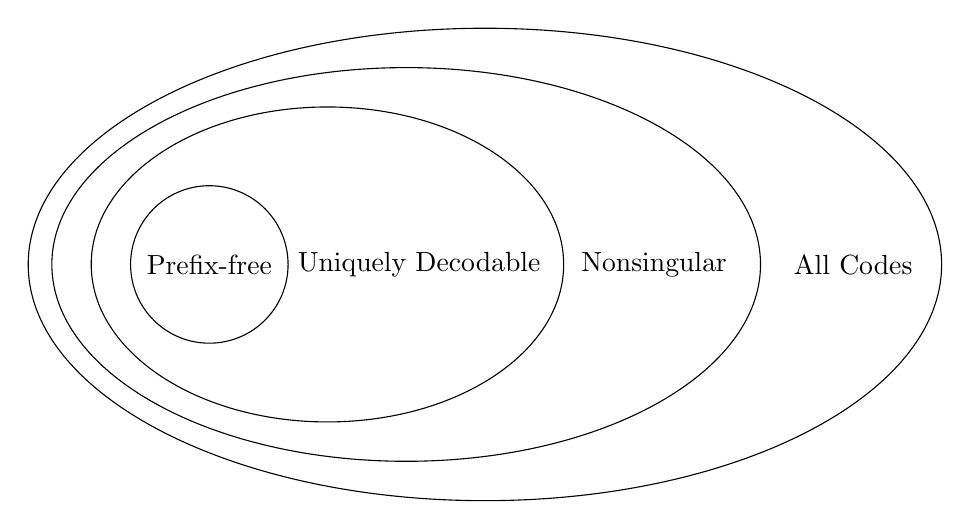
\begin{tikzpicture}
  % Draw the outer circle for "All Codes"
  \draw (3,0) ellipse (5.8cm and 3cm) node[right,xshift=3.8cm] {All Codes};

  % Draw the middle circle for "Nonsingular Codes"
  \draw (2,0) ellipse (4.5cm and 2.5cm) node[right,xshift=2.1cm] {Nonsingular};

  % Draw the inner circle for "Uniquely Decodable Codes"
  \draw (1,0) ellipse (3cm and 2cm) node[right, xshift=-0.5cm] {Uniquely Decodable};

  % Draw the most inner circle for "Prefix-free Codes"
  \draw (-0.5,0) ellipse (1cm and 1cm) node {Prefix-free};

\end{tikzpicture}
\caption{\label{fig:Classification-Codes}Classification of Codes}
\end{figure}

% \begin{figure}[t]
% \centering
% \begin{tikzpicture}
%   % Draw the outer circle for "All Codes"
%   \draw (3,0) ellipse (6cm and 3cm) node[right,xshift=3.8cm] {All Codes};

%   % Draw the middle circle for "Nonsingular Codes"
%   \draw (2,0) ellipse (4.5cm and 2.5cm) node[right,xshift=2.1cm] {Nonsingular};

%   % Draw the inner circle for "Uniquely Decodable Codes"
%   \draw (1,0) ellipse (3cm and 2cm) node[right, xshift=-0.5cm] {Uniquely Decodable};

%   % Draw the most inner circle for "Prefix-free Codes"
%   \draw (-0.5,0) ellipse (1cm and 1cm) node {Prefix-free};

% \end{tikzpicture}
% \caption{\label{fig:Classification-Codes}Classification of Codes}
% \end{figure}

%
% Section: Kraft Inequality
%

\section{Kraft Inequality}

The Kraft inequality provides a condition for the existence of a prefix-free code given a set of code word lengths. Kraft's inequality states that for a given set of code word lengths in a binary code, the sum of the reciprocals of powers of two corresponding to the code word lengths must be less than or equal to one. This condition is both necessary and sufficient: any prefix-free code must satisfy this inequality, and given a set of lengths that meets this condition, it is always possible to construct a corresponding prefix-free code. The elegance and utility of Kraft's inequality lie in its ability to link the lengths of code words with probabilistic structure.

\begin{figure}[t]
\centering
\begin{tikzpicture}[grow=right,->,>=stealth',level/.style={sibling distance = 3.2cm/#1,
  level distance = 2.5cm}] 
\node [circle,draw] (n1){}
    child{node [circle,draw] (n2) {$0$}
    }
    child{node [circle,draw] (n3) {$1$}
        child{node [circle,draw] (n4) {$10$}}
        child{node [circle,draw] (n5) {$11$}
            child{node [circle,draw] (n6) {$110$}}
            child{node [circle,draw] (n7) {$111$}
                child{node [circle,draw] (n8) {$1110$}}
            }
        }
    };
    
% Now, we add the edge labels
\path (n1) -- (n2) node [midway, above]  {$0$};
\path (n1) -- (n3) node [midway, above] {$1$};
\path (n3) -- (n4) node [midway, above]  {$0$};
\path (n3) -- (n5) node [midway, above] {$1$};
\path (n5) -- (n6) node [midway, above] {$0$};
\path (n5) -- (n7) node [midway, above] {$1$};
\path (n7) -- (n8) node [midway, above] {$0$};
\end{tikzpicture}
\caption{\label{fig:Prefix-Free-Tree}Prefix-free Tree}
\end{figure}

% \begin{figure}[t]
% \centering
% \begin{tikzpicture}[grow=right,->,>=stealth',level/.style={sibling distance = 4cm/#1,
%   level distance = 3cm}] 
% \node [circle,draw] (n1){}
%     child{node [circle,draw] (n2) {$0$}
%     }
%     child{node [circle,draw] (n3) {$1$}
%         child{node [circle,draw] (n4) {$10$}}
%         child{node [circle,draw] (n5) {$11$}
%             child{node [circle,draw] (n6) {$110$}}
%             child{node [circle,draw] (n7) {$111$}
%                 child{node [circle,draw] (n8) {$1110$}}
%             }
%         }
%     };
    
% % Now, we add the edge labels
% \path (n1) -- (n2) node [midway, above]  {$0$};
% \path (n1) -- (n3) node [midway, above] {$1$};
% \path (n3) -- (n4) node [midway, above]  {$0$};
% \path (n3) -- (n5) node [midway, above] {$1$};
% \path (n5) -- (n6) node [midway, above] {$0$};
% \path (n5) -- (n7) node [midway, above] {$1$};
% \path (n7) -- (n8) node [midway, above] {$0$};
% \end{tikzpicture}
% \caption{\label{fig:Prefix-Free-Tree}Prefix-free Tree}
% \end{figure}

\begin{theorem}[Kraft Inequality]
\label{th:Kraft-Inequality}
\index{Kraft's inequality}
Let $\mathcal{L}=\left\{ l_{1},l_{2},\ldots,l_{q}\right\}$ be a set of lengths, where $l_{i}\in\mathbb{N}$, then there exists a binary prefix-free code $C$ whose code words have the lengths of $\mathcal{L}$ if, and only if,
\[
\sum_{l_{i}\in\mathcal{L}}2^{-l_{i}}\leq1
\]
\end{theorem}
\begin{proof}
Consider a binary tree whose branches are labeled with the symbols of the code alphabet, in such a way that the path from the root to the leaves traces out the symbols of a code word. The prefix-free condition implies that nodes representing complete code words cannot have descendants. An example of such a tree, for the code described in Example \ref{ex:prefix-free}, is shown in Figure \ref{fig:Prefix-Free-Tree}.

Let $l_{max}=\max \left\{ l_{1},l_{2},\ldots,l_{q}\right\}$, that is, the length of the longest code word from the set of lengths. There will be at most $2^{l_{max}}$ leaf nodes in the tree, but at level $l_{i}$ we have to prune $2^{l_{max} - l_{i}}$ leaves, since the code is prefix-free. Summing over all the code words' lengths, we have that the total number of pruned leaves must be less than or equal to the maximum number of leaves, that is
\[
\sum_{l_{i}\in\mathcal{L}}2^{l_{max}-l_{i}} \leq 2^{l_{max}}
\]
or, equivalently,
\[
\sum_{l_{i}\in\mathcal{L}}2^{-l_{i}} \leq 1
\]
which is exactly the inequality we are trying to prove.

Conversely, given any set of code words' lengths $\mathcal{L}=\left\{ l_{1},l_{2},\ldots,l_{q}\right\}$ that satisfy the Kraft inequality, we can always construct a binary tree, like the one in the Figure \ref{fig:Prefix-Free-Tree}. Label the first node (lexicographically) of depth $l_{1}$ as code word 1, and remove its descendants from the tree. Then label the first remaining node of depth $l_{2}$ as code word 2, and so on. Proceeding this way, we construct a prefix code with the specified lengths.
\end{proof}

Given a code $C$ whose code word lengths $\mathcal{L}$ satisfy the Kraft inequality does not necessarily mean that the code is prefix-free, since what the inequality states is that there exists a prefix-free code with those word lengths, not that all codes with those word lengths are prefix-free.

\begin{example}
\label{ex:not-prefix-fix}
The code $C(a)=0$, $C(b)=111$, $C(c)=110$ and $C(d)=100$ satisfies the Kraft inequality, but it is not prefix-free.
\end{example}

McMillan's inequality extends Kraft's bound to all uniquely decodable codes: any such code with lengths \(l_i\) satisfies \(\sum_i 2^{-l_i}\le 1\). Combined with Kraft's theorem, this means a set of lengths meets this inequality if and only if it can be realized by a prefix-free---and thus uniquely decodable---code.

\begin{theorem}[McMillan's Inequality]
\index{McMillan's Inequality}
\label{th:McMillan-Inequality}
Let $\mathcal{L}=\left\{ l_{1},l_{2},\ldots,l_{q}\right\}$ be a set of lengths, where $l_{i}\in\mathbb{N}$, then there exists a uniquely decodable code $C$ whose code words have the lengths of $\mathcal{L}$ if, and only if,
\[
\sum_{l_{i}\in\mathcal{L}}2^{-l_{i}} \leq 1
\]
\end{theorem}
\begin{proof}
Let $S=\sum_{i=1}^q 2^{-l_i}$. For each $n\in\mathbb{N}$, let $C^n$ be the set of all concatenations of $n$ code words. Because the code is uniquely decodable, distinct concatenations in $C^n$ produce distinct binary strings. Consider an infinite fair-coin binary sequence $X=(X_1,X_2,\ldots)$, and for any finite binary string $u$ write $[u]=\{X:\, X \text{ begins with } u\}$. Then $\mathbb{P}([u])=2^{-|u|}$, and the cylinder sets $\{[w]: w\in C^n\}$ are pairwise disjoint. Therefore,
\[
\sum_{w\in C^n} 2^{-|w|} \;=\; \sum_{w\in C^n} \mathbb{P}([w]) \;\le\; 1.
\]
But the left-hand side factors as
\[
\sum_{w\in C^n} 2^{-|w|} \;=\; \Big(\sum_{i=1}^q 2^{-l_i}\Big)^n \;=\; S^n.
\]
Hence $S^n\le 1$ for all $n$, which implies $S\le 1$.
\end{proof}

In the theory of nescience, we focus on prefix-free codes without loss of generality: every uniquely decodable code satisfies Kraft's inequality, so there exists a prefix-free code with the same code-word lengths.

\begin{corollary}
There is an instantaneous (prefix-free) code with word lengths $l_1, \ldots, l_q$ if and only if there is a uniquely decodable code with these word lengths.
\end{corollary}
\begin{proof}
Every prefix-free code is uniquely decodable.

If a uniquely decodable code exists with lengths $l_1,\ldots,l_q$, then by McMillan's inequality $\sum_i 2^{-l_i}\le 1$. By Theorem \ref{th:Kraft-Inequality} (sufficiency), there exists a prefix-free code with the same lengths.
\end{proof}

In the context of nescience, our interest lies not in particular code assignments but in the multiset of code word lengths. This emphasis lets us abstract away from code construction details and focus on the mathematical properties of lengths, which are central to the measures we will use.

%
% Section: Optimal Codes
%

\section{Optimal Codes}
\label{sec:Optimal-Codes}

In coding theory, a compact code is an optimal encoding strategy that minimizes the expected length of code words, a concept central to evaluating a code's efficiency. The expected length of a code is determined by the weighted average of the lengths of its code words, with weights corresponding to the probability distribution of the source symbols. By designing code words so that more frequent symbols are assigned shorter lengths and less frequent ones longer lengths, compact codes effectively reduce the average size needed to encode information. This principle is pivotal in data compression, as it allows for a significant reduction in the space required for storage or the bandwidth needed for transmission.

Let $\mathcal{S}=\{ s_{1},\ldots,s_{q}\}$ be a finite source alphabet, and let $P$ be a probability distribution on $\mathcal{S}$.

\begin{definition}
The \emph{expected length}\index{Expected length of a code} of a code $C$, denoted by $L_{C}$, is
\[
L_{C} \;=\; \sum_{i=1}^{q} P(s_{i})\,l_{i},
\]
where $\mathcal{L} = \{ l_{1},\ldots,l_{q}\}$ are the code-word lengths of $C$. We may simply write $L$ when $C$ is clear from context.
\end{definition}

Our goal is to identify a code $C$ that minimizes $L$ under $P$. Such a code is optimal for $\mathcal{S}$ and $P$.

Compact codes achieve the lowest possible weighted average codeword length.

\begin{definition}
A code $C$ is \emph{compact}\index{Compact code} (optimal) if, for the given source alphabet $\mathcal{S}$ and distribution $P$, its expected length $L_{C}$ is minimal among all codes over the same code alphabet.
\end{definition}

The existence of compact codes for all possible source alphabets is a foundational aspect of coding theory, suggesting that for every finite source alphabet, an optimally efficient encoding scheme can be devised.

\begin{proposition}
For every finite source alphabet $\mathcal{S}$ and distribution $P$ there exists at least one code $C$ that is compact.
\end{proposition}
\begin{proof}
Huffman's algorithm (see Section \ref{sec:Huffman-Algorithm}) constructs a prefix-free code that minimizes the expected length for the given $P$. Hence an optimal code exists.
\end{proof}

It is convenient to distinguish between \emph{coding efficiency} and \emph{redundancy} relative to the source entropy. Let $H_r(P)=-\sum_i P(s_i)\log_r P(s_i)$ be the $r$-ary entropy (logarithms base $r$, where $r$ is the code alphabet size).

\begin{definition}
The \emph{coding efficiency} is
\[
\eta \;=\; \frac{H_r(P)}{L}\in(0,1],
\]
and the (normalized) \emph{redundancy} is
\[
\rho \;=\; 1-\eta \;=\; \frac{L-H_r(P)}{L}\in[0,1).
\]
\end{definition}

Our aim is to \emph{maximize} efficiency (equivalently, \emph{minimize} redundancy). Note that $L\ge H_r(P)$ (Theorem \ref{th:optimal_codes} below), so $\eta\le 1$.

Next theorem states that the entropy of the probability distibution $P$ poses a limit to the average length of prefix-free codes.

\begin{theorem}
\label{th:optimal_codes}
For any prefix-free $r$-ary code with lengths $\{l_i\}$ and source distribution $P$,
\[
H_{r}(P) \;\le\; L \;=\; \sum_{i=1}^{q} P(s_i)l_i,
\]
with equality if and only if $r^{-l_{i}} = P(s_i)$ for all $i$.
\end{theorem}
\begin{proof}
Let $\alpha=\sum_{i} r^{-l_i}\le 1$ by Kraft's inequality. Define a probability distribution $\tilde{Q}$ by
\[
\tilde{Q}(s_i)\;=\;\frac{r^{-l_i}}{\alpha}.
\]
Then
\begin{equation*}
\begin{split}
L - H_r(P)
& = \sum_i P(s_i)\Big(l_i + \log_r P(s_i)\Big) \\
& = \sum_i P(s_i)\log_r\!\Big(\frac{r^{l_i}P(s_i)}{1}\Big)
= \sum_i P(s_i)\log_r\!\Big(\frac{P(s_i)}{r^{-l_i}}\Big).
\end{split}
\end{equation*}
Write $r^{-l_i}=\alpha\,\tilde{Q}(s_i)$ to get
\begin{equation*}
\begin{split}
L - H_r(P)
& = \sum_i P(s_i)\log_r\!\Big(\frac{P(s_i)}{\tilde{Q}(s_i)}\Big)
\;+\; \log_r\!\Big(\frac{1}{\alpha}\Big) \\
& = D_r\!\big(P\;\|\;\tilde{Q}\big) \;+\; \log_r(1/\alpha)\;\ge\;0,
\end{split}
\end{equation*}
since the $r$-ary Kullback–Leibler divergence $D_r$ is nonnegative and $\alpha\le 1$. Equality holds iff both terms vanish, i.e., $\alpha=1$ and $P=\tilde{Q}$, which is equivalent to $r^{-l_i}=P(s_i)$ for all $i$.
\end{proof}

In data compression we are particularly interested in $r$-adic distributions.

\begin{definition}
A distribution $P$ is called \emph{$r$-adic} if each $P(s_i)$ is an exact $r$-adic probability, i.e., $P(s_i)=r^{-n_i}$ for some integers $n_i \ge 0$.
\end{definition}

Equality in Theorem \ref{th:optimal_codes} occurs precisely for sources whose symbol probabilities are exact powers of $r^{-1}$.

\begin{corollary}
Equality $L=H_r(P)$ in Theorem \ref{th:optimal_codes} holds if and only if $P$ is $r$-adic (equivalently, there exists a prefix-free code with $l_i=-\log_r P(s_i)$).
\end{corollary}
\begin{proof}
Theorem \ref{th:optimal_codes} shows equality holds exactly when $r^{-l_i}=P(s_i)$ for all $i$, i.e., when each $P(s_i)$ is an $r$-adic probability.
\end{proof}

In analysis it is natural to consider the \emph{ideal} real-valued lengths $\ell_i^\ast=-\log_r P(s_i)$, which need not be integers. Choosing integer lengths $l_i=\lceil \ell_i^\ast\rceil$ yields a feasible prefix-free code (by Kraft) with near-optimal average length.

\begin{proposition}[Shannon–Fano bound]
For $l_i=\lceil -\log_r P(s_i)\rceil$,
\[
H_r(P) \;\le\; L \;<\; H_r(P)+1.
\]
\end{proposition}
\begin{proof}
By definition $l_i< -\log_r P(s_i)+1$, hence
\[
L=\sum_i P(s_i)l_i \;<\; \sum_i P(s_i)\big(-\log_r P(s_i)+1\big) \;=\; H_r(P)+1.
\]
Moreover, $\sum_i r^{-l_i}\le \sum_i r^{\log_r P(s_i)}=\sum_i P(s_i)=1$, so the lengths are feasible. The lower bound $L\ge H_r(P)$ is Theorem \ref{th:optimal_codes}.
\end{proof}

Kraft's inequality and expected length allow us to compare codes for a fixed source.

\begin{definition}
Let $C_1,C_2$ be two codes on $\mathcal{S}$ with expected lengths $L_{C_1},L_{C_2}$ under $P$. We say that $C_1$ is \emph{more efficient}\index{Code efficiency} than $C_2$ (for $P$) if $L_{C_1}\le L_{C_2}$, with strict inequality for at least one symbol probability configuration (equivalently, $L_{C_1}<L_{C_2}$ for the given $P$).
\end{definition}

\begin{example}
The non–prefix-free code in Example \ref{ex:not-prefix-fix} has lengths $(1,3,3,3)$, which satisfy Kraft's inequality. Therefore, there exists a prefix-free code with the \emph{same} lengths; for instance,
\[
C(a)=1,\quad C(b)=000,\quad C(c)=001,\quad C(d)=010.
\]
For many $P$, these lengths yield a smaller expected length than the prefix-free code of Example \ref{ex:prefix-free} (which has lengths $(1,2,3,4)$); the comparison is determined by $P$ via $L=\sum_i P(s_i)l_i$.
\end{example}

Intuitively, a prefix-free code is \emph{complete} if its set of code words cannot be augmented (by adding another code word) while preserving the prefix-free property.

\begin{definition}
A prefix-free code $C$ is \emph{complete}\index{Complete code} if there does not exist a binary string $w$ such that $C\cup\{w\}$ is still prefix-free.
\end{definition}

Kraft's inequality characterizes completeness.

\begin{proposition}
A prefix-free code $C$ with lengths $\mathcal{L}=\{l_1,\ldots,l_q\}$ is complete if and only if
\[
\sum_{i=1}^q 2^{-l_i}=1.
\]
\end{proposition}
\begin{proof}
If the sum is $<1$, there remains unused capacity in the binary tree at some depth, so one can add at least one more leaf without violating prefix-freeness, contradicting completeness. Conversely, if the sum equals $1$, the descendant subtrees of the selected leaves exactly partition the leaf set at some depth; no additional leaf can be added without creating a prefix conflict.
\end{proof}

%
% Section: Entropy
%

\section{Entropy}
\label{sec:Entropy}

In this section we introduce \emph{entropy} as a measure of the uncertainty of a discrete random variable. Entropy appears in many contexts (communications, statistics, finance, etc.); here it is important because it will allow us to identify codes with the shortest possible average length.

Let $A=\{a_1,a_2,\ldots,a_n\}$ be a finite set, and let $X$ be a random variable on $A$ with probability mass function $p(a)$.

\begin{definition}[Entropy]
The \emph{entropy}\index{Entropy} of $X$, denoted $H(X)$ and measured in \emph{bits}\index{Bit}, is
\[
H(X)=\sum_{a\in A} p(a)\,\log\frac{1}{p(a)}.
\]
\end{definition}

Entropy depends only on the probabilities $\{p(a)\}$, not on the labels in $A$. Clearly $H(X)\ge 0$ since $0\le p(a)\le 1$ implies $-\log p(a)\ge 0$. If $p(a_i)=0$ for some $i$, the corresponding summand is taken to be $0$, consistent with $\lim_{p\to 0^+} p\log(1/p)=0$. If we change the logarithm base to $u$, entropy scales by a factor $\log_u 2$ (see Equation \ref{eq:change_base_logarithm}).

\begin{example}
Let $X$ a random variable defined over the set $A = \{a_1, a_2\}$, with values $p(a_1) = q$ and $p(a_2) = 1-q$. Then, the entropy of $X$ is given by:
\[
H(X) = q \log \frac{1}{q} + (1-q) \log \frac{1}{1-q}
\]
Figure \ref{fig:entropy_function} shows the entropy of $X$ for different values of $q$. If $q=0$ or $q=1$ the entropy is 0, that is, there is no uncertainty about which value of $A$ we will get. The maximum value of $H$ is 1, and it is reached when $q=1/2$; that is, we could say that 1 bit is the uncertainty associated to two equally probable symbols.
\end{example}

\begin{figure}[h]
\centering\includegraphics[scale=0.4]{entropy_function}
\caption{\label{fig:entropy_function}Binary Entropy Function}
\end{figure}

The next proposition shows that entropy is maximized by the uniform distribution and that the maximum equals the logarithm of the alphabet size.

\begin{proposition}
\label{prop:maximum_entropy}
For $X$ on $A$ with $d(A)=n$, we have $H(X)\le \log n$, with equality if and only if $p(a_1)=\cdots=p(a_n)=1/n$.
\end{proposition}
\begin{proof}
Compute
\[
\log n - H(X)
= \sum_{i=1}^n p(a_i)\log n - \sum_{i=1}^n p(a_i)\log\frac{1}{p(a_i)}
= \sum_{i=1}^n p(a_i)\,\log\!\big(n\,p(a_i)\big).
\]
Using the change-of-base formula,
\[
\log n - H(X)
= (\log e)\sum_{i=1}^n p(a_i)\,\ln\!\big(n\,p(a_i)\big).
\]
By the inequality $\ln x \le x-1$, applied with $x=\frac{1}{n\,p(a_i)}$, we have
\[
\ln\!\big(n\,p(a_i)\big)\;\ge\; 1-\frac{1}{n\,p(a_i)}.
\]
Hence
\[
\log n - H(X)
\;\ge\; (\log e)\sum_{i=1}^n p(a_i)\!\left(1-\frac{1}{n\,p(a_i)}\right)
= (\log e)\Big(1-\tfrac{1}{n}\sum_{i=1}^n 1\Big)=0.
\]
Equality holds iff $\ln(n\,p(a_i))=0$ for all $i$, i.e., $p(a_i)=1/n$.
\end{proof}

\begin{example}
If we select a symbol from $A$ according to $p$, the entropy $H(X)$ is the minimum expected number of binary (Yes/No) questions required to identify the symbol. For equiprobable symbols this expected number is maximal and equals $\log |A|$.
\end{example}

% Joint entropy

We can extend the concept of entropy to a pair of random variables by means of using the joint probability mass function. In this way, the joint entropy will be a measure of the uncertainty associated to both variables. Let $A = \{a_1, a_2, \ldots, a_n\}$ and $B = \{b_1, b_2, \dots, b_m\}$ two finite sets, and $X$ and $Y$ two random variables defined over the sets $A$ and $B$ respectively, with probability mass function $p(a)$ and $p(b)$, and joint probability mass function $p(a, b)$.

\begin{definition}
The \emph{joint entropy} of the random variables $A$ and $B$, denoted by $H(A, B)$, is defined as:
\[
H(A, B) = \sum_{a \in A} \sum_{b \in B} p(a, b) \log \frac{1}{p(a, b)}
\]
\end{definition}

Joint entropy is symmetric: $H(A, B)=H(B, A)$, since the double sum is unchanged by swapping $a$ and $b$. The definition extends to any finite tuple $(A_1, \ldots, A_k)$ via the joint mass function $p(a_1, \ldots, a_k)$.

Adding a second random variable with an unknown outcome may increase entropy, as the following proposition shows.

\begin{proposition}
We have that
\[
H(A, B) \geq \max \left( H(A), H(B) \right)
\]
\end{proposition}
\begin{proof}
Because $\sum_{b}p(a,b)=p(a)$, we have $p(a,b)\le p(a)$ for all $a,b$, hence $\log\frac{1}{p(a,b)}\ge \log\frac{1}{p(a)}$. Therefore,
\begin{equation*}
\begin{split}
H(A, B) & = \sum_{a,b} p(a,b)\log\frac{1}{p(a,b)}
\;\ge\; \sum_{a,b} p(a,b)\log\frac{1}{p(a)} \\
& = \sum_{a} p(a)\log\frac{1}{p(a)}=H(X).
\end{split}
\end{equation*}
The inequality $H(A, B)\ge H(B)$ is analogous. Taking the maximum yields the claim.
\end{proof}

The joint entropy of two variables cannot exceed the sum of their individual entropies.

\begin{proposition}
\label{prop:joint_entropy}
We have $H(A, B)\le H(A) + H(B)$, with equality if and only if $A$ and $B$ are independent (i.e., $p(a,b)=p(a)p(b)$ for all $a,b$).
\end{proposition}
\begin{proof}
By Gibbs' inequality (which follows from $\ln x\le x-1$),
\begin{equation*}
\begin{split}
0 \;\le\; \sum_{a,b} p(a,b)\,\log\frac{p(a,b)}{p(a)p(b)}
& = \sum_{a,b} p(a,b)\log p(a,b) \\
& - \sum_{a,b} p(a,b)\log p(a) - \sum_{a,b} p(a,b)\log p(b).
\end{split}
\end{equation*}
Rearranging and recognizing the entropies,
\[
0 \;\le\; -H(A, B) + H(A) + H(B),
\]
which gives $H(A, B) \le H(A) + H(B)$. Equality in Gibbs' inequality holds if and only if $p(a,b)=p(a)p(b)$ for all $a,b$, i.e., when $A$ and $B$ are independent.
\end{proof}

% Conditional Entropy

The next concept derived from entropy is conditional entropy. It measures the remaining uncertainty about one random variable once the outcome of another is known.

\begin{definition}
The \emph{conditional entropy} of the random variable $B$ given the random variable $A$, denoted by $H(B \mid A)$, is defined as:
\[
H(B \mid A) = \sum_{a \in A} \sum_{b \in B} p(a, b) \log \frac{1}{p(b \mid a)}
\]
\end{definition}

In general $p(b\mid a)\neq p(a\mid b)$, so $H(B \mid A)\neq H(A \mid B)$. We have $H(B \mid A) = 0$ if and only if $B$ is (almost surely) a function of $A$.

The next proposition formalizes that conditioning cannot increase uncertainty.

\begin{proposition}
Given the random variables $X$ and $Y$, we have that $H(Y \mid X) \leq H(Y)$, and $H(Y \mid X) = H(Y)$ if, and only if, $p(a)$ and $p(b)$ are independent.
\end{proposition}
\begin{proof}
\begin{equation*}
\begin{split}
H(Y \mid X) & = \sum_{a \in A} \sum_{y \in B} p(a, b) \log \frac{1}{p(b \mid a)} = \sum_{a \in A} \sum_{b \in B} p(a, b) \log \frac{p(a)}{p(a, b)} \\
& = \sum_{a \in A} \sum_{b \in B} p(a, b) \log p(a) - \sum_{a \in A} \sum_{b \in B} p(a, b) \log p(a, b) \\
& = -H(X) + H(X, Y)
\end{split}
\end{equation*}
By Proposition \ref{prop:joint_entropy}, $H(X,Y)\le H(X)+H(Y)$, hence $H(Y\mid X)\le H(Y)$. Equality holds if and only if $H(X,Y)=H(X)+H(Y)$, i.e., $X$ and $Y$ are independent.
\end{proof}

From an intuitive standpoint, the uncertainty of a pair $(X,Y)$ should equal the uncertainty of $X$ plus the remaining uncertainty of $Y$ after observing $X$. This is the \emph{chain rule}.

\begin{proposition}[Chain rule]
\label{prop:chain_rule_entropy}
For any discrete $X,Y$, $H(X,Y)=H(X)+H(Y\mid X)$.
\end{proposition}
\begin{proof}
\begin{equation*}
\begin{split}
H(Y, X) & = \sum_{a \in A} \sum_{b \in B} p(a, b) \log \frac{1}{p(a, b)} = \sum_{a \in A} \sum_{b \in B} p(a, b) \log \frac{1}{p(a) p(a \mid b)} \\
& = \sum_{a \in A} \sum_{b \in B} p(a, b) \log \frac{1}{p(a)} + \sum_{a \in A} \sum_{b \in B} p(a, b) \log \frac{1}{p(a \mid b)} \\
& = H(X) + H(Y \mid X)
\end{split}
\end{equation*}
\end{proof}

% Mutual information

The last derived concept of entropy we are going to see is mutual information. Intuitively, the mutual information of two random variables $X$ and $Y$ measures the information that $X$ and $Y$ share, that is, how much knowing one of these variables reduces the uncertainty about the other.

\begin{definition}
The \emph{mutual information} of the random variable $X$ and $Y$, denoted by $I(X ; Y)$, is defined as:
\[
I(X ; Y) = \sum_{a \in A} \sum_{b \in B} p(a, b) \log \frac{p(a, b)}{p(a) p(b)}
\]
\end{definition}

Since $p(a, b) = p(b, a)$ we have that $I(X ; Y) = I(Y ; X)$, that is, the order of the random variables does not affect the concept of mutual information.

Next proposition shows that mutual information is a positive quantity, and it is equal to 0 if, and only if, the random variables are independent.

\begin{proposition}
For any discrete random variables $X$ and $Y$ we have that $I(X ; Y) \geq 0$, and $I(X ; Y) = 0$ if, and only if, the variables $X$ and $Y$ are independent.
\end{proposition}
\begin{proof}
Interpret $I(X;Y)$ as the Kullback-Leibler divergence
\[
I(X;Y)= D\big(p_{X,Y}\,\|\,p_Xp_Y\big)\;=\;\sum_{a,b} p(a,b)\,\log\frac{p(a,b)}{p(a)p(b)}\;\ge\;0
\]
by Gibbs' inequality, with equality if and only if $p(a,b)=p(a)p(b)$ for all $a,b$.
\end{proof}

Mutual information admits several equivalent forms that make its operational meaning explicit: it quantifies the reduction in uncertainty achieved by observing one variable about the other. Using the chain rule $H(X,Y)=H(X)+H(Y\mid X)=H(Y)+H(X\mid Y)$, we obtain the identities below, showing that $I(X;Y)$ is exactly the decrease in entropy of $X$ due to $Y$ (and symmetrically for $Y$).

\begin{proposition}
For any discrete random variables $X$ and $Y$, we have that:
\[
I(X;Y) = H(X) - H(X \mid Y) = H(Y) - H(Y \mid X)
\]
\end{proposition}
\begin{proof}
By the chain rule, $H(X,Y)=H(Y)+H(X\mid Y)$. Substituting into
\[
I(X;Y)=\sum_{a,b} p(a,b)\log\frac{p(a,b)}{p(a)p(b)}
= -H(X,Y)+H(X)+H(Y),
\]
we obtain $I(X;Y)=H(X)-H(X\mid Y)$. The other identity follows by symmetry.
\end{proof}

Another equivalent form of mutual information is its “inclusion-exclusion” expression: the sum of the marginal entropies minus the joint entropy. It follows immediately by substituting $H(X\mid Y)=H(X,Y)-H(Y)$ (or symmetrically $H(Y\mid X)=H(X,Y)-H(X)$) into $I(X;Y)=H(X)-H(X\mid Y)$, and highlights the Venn-diagram overlap interpretation.

\begin{proposition}
For any discrete random variables $X$ and $Y$, we have that:
\[
I(X;Y) = H(X) + H(Y) - H(X, Y)
\]
\end{proposition}
\begin{proof}
Combine $I(X;Y)=H(X)-H(X\mid Y)$ with $H(X\mid Y)=H(X,Y)-H(Y)$ (chain rule), yielding
$I(X;Y)=H(X)+H(Y)-H(X,Y)$.
\end{proof}

A useful sanity check is the self-information case. Since observing $S$ reveals $S$ completely, the remaining uncertainty $H(S\mid S)$ is zero; hence the mutual information of a variable with itself equals its entropy, as stated below.

\begin{proposition}
For any discrete random variable $S$ we have that $I(S;S)=H(S)$.
\end{proposition}
\begin{proof}
By the identity $I(X;Y)=H(X)-H(X\mid Y)$ with $X=Y=S$,
\[
I(S;S)=H(S)-H(S\mid S)=H(S)-0=H(S).
\]
\end{proof}

\begin{example}
Let $X\sim\mathrm{Bernoulli}(1/2)$ and let $Y=X\oplus N$, where $N\sim\mathrm{Bernoulli}(\varepsilon)$ is independent noise ($\oplus$ is XOR). Then $H(X)=H(Y)=1$, and
\[
H(X\mid Y)=H_\mathrm{b}(\varepsilon):=-\varepsilon\log\varepsilon-(1-\varepsilon)\log(1-\varepsilon),\qquad
I(X;Y)=1-H_\mathrm{b}(\varepsilon).
\]
For instance, with $\varepsilon=0.1$, $H_\mathrm{b}(0.1)\approx 0.469$, so $I(X;Y)\approx 0.531$ bits. A Venn diagram interpretation: the circle areas represent $H(X)$ and $H(Y)$, the overlap is $I(X;Y)$, and the non-overlapping parts are $H(X\mid Y)$ and $H(Y\mid X)$.
\end{example}

Figure \ref{fig:venn-entropy} provides Venn-style schematic for entropies, conditional entropies and mutual information.

\begin{figure}[h]
\label{fig:venn-entropy}
\centering
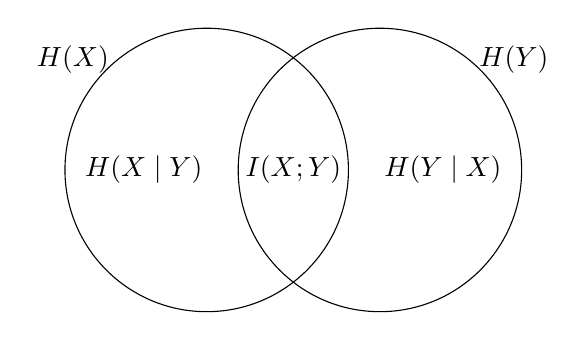
\begin{tikzpicture}[scale=1.0]
\def\r{1.8}
\draw (0,0) circle (\r);
\draw (2.2,0) circle (\r);
\node at (-1.7,1.4) {$H(X)$};
\node at (3.9,1.4) {$H(Y)$};
\node at (1.1,0) {$I(X;Y)$};
\node at (-0.8,0) {$H(X\mid Y)$};
\node at (3.0,0) {$H(Y\mid X)$};
\end{tikzpicture}
\caption{$H(X)$ and $H(Y)$ with overlap $I(X;Y)$.}
\end{figure}

%
% Section: Huffman Algorithm
%

\section{Huffman Algorithm}
\label{sec:Huffman-Algorithm}

From a practical point of view, there exists an algorithm, called \emph{Huffman algorithm}, that provides a method to build compact prefix-free codes given a probability distribution. For simplicity, we will study first the particular case of constructing binary prefix-free codes, and later I will provide its generalization to the case of D-ary prefix-free codes.

\begin{algorithm}
\caption{Huffman Algorithm}
\label{alg:Huffman}
\begin{algorithmic}
\Procedure{Huffman}{$Q$}
    \State $T \gets$ empty tree
    \For {$i \gets 1, d(Q) - 1$}
        \State allocate a new node $z$
        \State z.left = x = EXTRACT-MIN(Q)
        \State z.rigth = y = EXTRACT-MIN(Q)
        \State z.freq = x.freq + y.freq
        \State INSERT(Q, z)
    \EndFor
    \State \textbf{return} $T$
\EndProcedure
\end{algorithmic}
\end{algorithm}

The algorithm (see Algorithm \ref{alg:Huffman}) expects as input a source alphabet $\mathcal{S}=\left\{ s_{1},s_{2},\ldots,s_{q}\right\}$ and their corresponding probabilities $P = \left\{ p_{1}, p_{2}, \ldots, p_{q} \right\}$. For simplicity, $Q = \left\{ (s_{1}, p_{1}), (s_{2}, p_{2}), \ldots, (s_{q}, p_{q}) \right\}$ will merge both sets into a single one. The algorithm works by constructing a binary tree $T$, similar to the one used in the proof of Theorem \ref{th:Kraft-Inequality}. The algorithm requires $d(Q) - 1$ iterations to finish. During each iteration, the two elements with the lowest probability are selected and removed from set $Q$, and a new tree node $z$ is created, with the addition of the removed values, and added to the set $Q$. Once the tree has been constructed, we have to perform a tree transversal assigning a $0$ to each left branch, and a $1$ to each right branch, until we reach a leaf.

\begin{example}
Assume we have the source alphabet $\mathcal{S}=\left\{a, b, c, d, e, f\right\}$ with the associated probabilities $P = \left\{0.35, 0.16, 0.08, 0.12, 0.06, 0.23 \right\}$. In Figure \label{fig:Huffman-Algorithm} are depicted the contents of the set $Q$ and the tree $T$ for each iteration of the algorithm. At the end of the algorithm, if we perform a traversal of the $T$ tree, we will get the following prefix-free compact code for the source alphabet $S$: 

\bigskip

\centering
\begin{tabular}{l l}
\toprule
\textbf{Source Word} & \textbf{Code Word} \\
\midrule
a & 11   \\
b & 00   \\
c & 1011 \\
d & 100  \\
e & 1010 \\
f & 01   \\
\bottomrule
\end{tabular}

\bigskip

% The expected length of the code is $L = 2.4$ , and its entropy is $\mathcal{H} \approx 2.34$. Since the set of probabilities is not D-adic ...

% % Q: Shall I mention the expected length of a uniform code?

\end{example}

% \begin{figure}[h]
% \centering\includegraphics[scale=0.5]{huffman}
% \caption{\label{fig:Huffman-Algorithm}Huffman Algorithm}
% \end{figure}

% \emph{This order is arbitrary; switching the left and rigth child of any node yields a different code of the same cost}

% % Lemma would be better

% \begin{proposition}
% Given the probability is ...
% \end{proposition}
% \begin{proof}
% {\color{red} TODO}
% \end{proof}

% The next theorem shows the optimality of the Huffman coding.

% \begin{theorem}
% If $C$ is a Huffman code then $C$ is compact.
% \end{theorem}
% \begin{proof}
% {\color{red} TODO}
% \end{proof}

% {\color{red} TODO: Rewrite the following paragraphs}

% \emph{So not only is this code optimal in the sense that no other feasible code performs better, but it is very close to the theoretical limit established by the entropy}

% \emph{Although we have proved the theorem for a binary alphabet, the proof can be extended to establishing optimality of the Huffam coding algorithm for a D-ary alphabet as well.}

% {\color{red} TODO: show how to extend the algorithm to D-ary codes}

% \emph{Then -ary Huffman algorithm uses the {0, 1, ..., n-1} alphabet to encode message and build an n-ary tree [...] the same algorithm applies as for binary codes, except that the n least probable symbols are taken together , instead of just the 2 least probable. Note that for n greater than 2, not all sets of source words  can properly form an n-ary tree for Huffman coding. In this case, additional 0-probability place holders must be added. This is because the tree must form and n to 1 contractor; for binary coding, this is a 2 to 1 contractor, and any sized set can form such a contractor. If the number fo source words is congruent to 1 module n-1, then the set of source words will form a proper Huffman tree.}

% {\color{red} Mention arithmetic coding}

%
% Discretization of Continuous Variables
%

\section{Discretization of Continuous Variables}
\label{sec:discretization_continuous_variables}

When summarizing large masses of raw data, it is often useful to distribute the data into classes, or categories, and to determine the number of individuals belonging to each class, called absolute frequency. The following definition formally introduces this concept.

\begin{definition}
Let $\mathcal{S}$ be a population consisting of $n$ individuals, and let a variable $X: \mathcal{S} \rightarrow \mathcal{D}$ represent the mapping of individuals in $\mathcal{S}$ to values in the set $\mathcal{D}$, where $k$ is the cardinality of $\mathcal{D}$. The \emph{absolute frequency}\index{Absolute frequency}, also known simply as \emph{frequency}, denoted by $n_i$ for $1 \leq i \leq k$, quantifies the number of individuals in $\mathcal{S}$ for which $X$ assigns the value corresponding to the $i$-th category of $\mathcal{D}$.
\end{definition}

The sum of the frequencies must be equal to population size, that is, $\sum_{i=1}^k n_i = n$.

If the variable $X$ is continuous, the elements of $\mathcal{D}$ are referred to as \emph{class intervals}\index{Class interval}. The endpoints of these intervals are known as \emph{class limits}\index{Class limits}; the smaller number is termed the \emph{lower class limit}\index{Lower class limit}, and the larger number, the \emph{upper class limit}\index{Upper class limit}. A \emph{class interval}\index{Class interval} that lacks either an upper or a lower class limit is known as an \emph{open class interval}\index{Open class interval}. The \emph{width}\index{Class interval width} of a class interval is defined as the difference between the upper and lower class boundaries, denoted by $a_i = e_i - e_{i-1}$. The \emph{class mark}\index{Class mark}, or the midpoint of a class interval, is calculated as $a_i = \frac{e_i + e_{i-1}}{2}$. It is assumed that all observations within a specific class interval are equivalent concerning their categorical assignment. Refer to Section \ref{sec:discretization_algorithms} for more information about how to discretize a continous variable into discrete intervals.

\begin{example}
In a study measuring adult heights within a community, researchers record heights ranging from 150 cm to 200 cm and organize them into 10 cm class intervals: 150-159 cm, 160-169 cm, 170-179 cm, 180-189 cm, and 190-199 cm. Each interval's lower and upper class limits are respectively the start and end points, such as 150 cm and 159 cm for the first interval. If the last interval had no specified upper limit, it would be considered an open class interval. The class width, typically 10 cm, is the operational span between boundaries, and the class mark, calculated as the midpoint of each interval (e.g., 154.5 cm for the first interval), provides a central value for summarizing data within that range.
\end{example}

A tabular arrangement of data by classes together with the corresponding class frequencies is called a frequency distribution, or frequency table.

\begin{definition}
Let $\mathcal{S}$ be a population consisting of $n$ individuals, and let $X: \mathcal{S} \rightarrow \mathcal{D}$ be a variable that maps individuals in $\mathcal{S}$ to $k$ distinct values of the set $\mathcal{D}$. A \emph{frequency distribution}\index{Frequency distribution} is represented the set of pairs $\{(d_i, n_i) : 1 \leq i \leq k\}$, where $d_i$ denotes the $i$-th interval and $n_i$ represents the number of individuals from $\mathcal{S}$ whose value under $X$ falls within the interval $d_i$.
\end{definition}

Frequency distributions are useful for statistical analysis and helps in visualizing data by grouping values, which simplifies the understanding of distribution and central tendencies within the data.

The relative frequency of a class is the frequency of the class divided by the total frequency of all classes

\begin{definition}
Let $\mathcal{S}$ be a population consisting of $n$ individuals, and let a variable $X: \mathcal{S} \rightarrow \mathcal{D}$ represent the mapping of individuals in $\mathcal{S}$ to values in the set $\mathcal{D}$, where $k$ is the cardinality of $\mathcal{D}$. The \emph{relative frequency}\index{Relative frequency}, denoted by $f_i$, is the ratio $f_i = \frac{n_i}{n}$ for $1 \leq i \leq k$.
\end{definition}

The sum of the relative frequencies is equal to one, that is, $\sum_{i=1}^k f_i = 1$.

The total frequency of all values less than the upper class boundary of a given class interval is called the cumulative frequency up to and including that class interval.

\begin{definition}
Let $\mathcal{S}$ be a population consisting of $n$ individuals, and let a variable $X: \mathcal{S} \rightarrow \mathcal{D}$ represent the mapping of individuals in $\mathcal{S}$ to values in the set $\mathcal{D}$, where $k$ is the cardinality of $\mathcal{D}$. The \emph{cumulative frequency}\index{Cumulative frequency}, denoted by $N_i$ for $1 \leq i \leq k$, represents the total number of individuals in $\mathcal{S}$ for which $X$ assigns a value less than or equal to the upper limit of the $i$-th category of $\mathcal{D}$. This is mathematically expressed as $N_i = \sum_{j=1}^i n_j$, where $n_j$ is the absolute frequency of the $j$-th category.
\end{definition}

By accumulating the frequencies up to each category or interval, cumulative frequencies provides a running total that shows how many data points fall below a certain value.

\subsubsection*{Discretization Algorithms}

Let $\mathcal{X}$ a continuous random variable that follows a probability density function $P_\mathcal{X}$, and assume we have collected $n$ independent and identically distributed samples $\bold{x} = \{x_1, \ldots, x_n\}$ from $\mathcal{X}$. We are interested in computing the length of a compressed version of $\bold{x}$ using an optimal compressor. Unfortunately, and except for some degenerate distributions, there is no lossless compression algorithm that produces a string with fewer bits than encoding directly the elements $\bold{x}$. Compression algorithms for continuous data only work in case that the elements of $\bold{x}$ are not independent, as it is the case with images or sound. But, if this is not the case, the only option available to compress $\bold{x}$ is to use a lossy compression algorithm, where some information is lost.

We are looking for an algorithm to produce a finite non-overlapping partition of $m$ discrete intervals $D=\{ [d_o, d_1], (d_1, d_2], \ldots, (d_{m-1}, d_m] \}$, where $d_o = \min{\bold{x}_j}$, and $d_m = \max{\bold{x}_j}$, and $d_i < d_{i+1}$ for $i = 0, 1, \ldots, m-1$, assign a unique label to each interval, and encode the elements of $\bold{x}$ using this labeling schema. As compression algorithm we will use an optimal length code given the relative frequencies of the labels in the encoded vector. In this sense, our goal is to have a collection of intervals with sufficiently number of samples (so they are statistically significant) and that the distribution of frequencies resembles the original probability distribution $P_\mathcal{X}$.

A discretization algorithm is a mapping between a (possibly huge) number of numeric values and a reduced set of discrete values, and so, it is a process in which some information is potentially lost. The choice of discretization algorithm is something that could have a high impact in the practical computation of the nescience. We are interested in a discretization algorithm that produces a large number of intervals (low bias), with a large number of number of observations per interval (low variance). Common techniques include \emph{equal width discretization}, \emph{equal frequency discretization} and \emph{fixed frequency discretization}. However, these techniques require the optimization of an hyperparameter, and so, they are not suitable for our purposes.

In a \emph{proportional discretization approach} the number of intervals $m$ and the number of observations per interval $s$ are equally proportional to the number of observations $n$. The algorithm starts by sorting the values of $\bold{x}_j$ in ascending order and then discretizing them into $m$ intervals of approximately $s$ (possibly identical) values each. In this way, as the number of training observations increases, both interval frequency and number of intervals increases, taking advantage of the larger number of observations. In the same way, when the number of observations decreases, we reduce both.

%
% References
%

\section*{References}

Core references for the chapter "Coding"

\cite{cover2012elements}: Cover and Thomas is the standard reference for modern information theory. It introduces entropy, mutual information, source and channel coding theorems, and provides the theoretical basis for coding.

\cite{abramson1963information}: Abramson's book is a classic early text that presents coding theory in an accessible way. It is useful for historical perspective and for understanding the development of the main coding ideas.

\cite{kraft1949device}: Kraft’s thesis introduces the Kraft inequality, a cornerstone result for the theory of uniquely decodable prefix codes.

\cite{mcmillan1956two}: McMillan extends Kraft's result to a more general form, establishing the Kraft-McMillan inequality fundamental to coding theory.

\cite{gersho2012vector}: Gersho and Gray provide the standard reference on quantization methods used in lossy compression, important for bridging coding theory with practical applications.

\cite{lloyd1982least}: Lloyd’s algorithm (often rediscovered as k-means) is a central method for quantization and lossy compression. It provides a concrete link between coding and clustering.

\cite{li2013introduction}: Li and Vitányi’s book is the definitive source on Kolmogorov complexity, linking coding theory with randomness and algorithmic information. It is essential for connecting coding to the broader framework of nescience.

% \begin{verbatim}

% % Rice's rule

% A common rule of thumb for determining the number of bins in a histogram is Rice’s rule, which suggests using approximately 2n^1/3 bins, where n is the sample size. This heuristic strikes a balance between over-smoothing and over-fitting and has been widely adopted in introductory statistics texts as a practical default choice for discretization \cite{freedman1978statistics}.

% Freedman, D., Pisani, R., & Purves, R. (1978). Statistics (2nd ed.). New York, NY: W. W. Norton. (Section 6.3: binning rules including “twice the cube root of n”).

% @book{freedman1978statistics,
%   title={Statistics},
%   author={Freedman, David and Pisani, Robert and Purves, Roger},
%   year={1978},
%   publisher={W. W. Norton \& Company}
% }

% % Jeffreys smoothing

% @article{krichevsky1981performance,
%   title={The performance of universal encoding},
%   author={Krichevsky, R. E. and Trofimov, V. K.},
%   journal={IEEE Transactions on Information Theory},
%   volume={27},
%   number={2},
%   pages={199--207},
%   year={1981},
%   publisher={IEEE}
% }

% To avoid degenerate estimates when computing code lengths from finite samples, we apply a Bayesian smoothing procedure known as the **Krichevsky-Trofimov (KT) estimator**, also called **Jeffreys prior smoothing**. This method assigns a prior weight of $1/2$ to each possible outcome, resulting in probability estimates of the form $(n_i+1/2)/(N + k/2)$, where $n_i$ is the count of symbol $i$, $N$ the sample size, and $k$ the alphabet size. This estimator was introduced in the information theory literature by Krichevsky and Trofimov\~\cite{krichevsky1981performance}, and it is known to yield nearly optimal universal coding performance.

% % Trimmed core range

% @book{huber1981robust,
%   title={Robust Statistics},
%   author={Huber, Peter J.},
%   year={1981},
%   publisher={John Wiley \& Sons}
% }
% When discretizing continuous variables, extreme outliers can distort the binning process, leading to empty or uninformative intervals. To address this, we use a **trimmed core range**, where a small fraction (e.g., 0.5\%) of the data at each tail is excluded when defining the binning range. This approach comes from the broader field of **robust statistics**, which develops methods that are less sensitive to outliers. The idea of trimming as a robustness technique was systematically developed in Huber's classic monograph\~\cite{huber1981robust}.

% \end{verbatim}






%
% CHAPTER: Algorithmic Information
%

%
% CHAPTER 4.- Kolmogorov Complexity
%

% TODO: Can we talk about independent topics? K(t|s) = K(t)
% TODO: Does K(t|s) != K(s|t)?


\chapterimage{Mandelbrot.pdf}

\chapter{Complexity}
\label{chap:Algorithmic_Information}

\begin{quote}
\begin{flushright}
\emph{An approximate answer to the right problem  \\
is worth a good deal more than \\
an exact answer to an approximate problem. \\}
John Tukey
\end{flushright}
\end{quote}
\bigskip

In Appendix \ref{chap:Coding}, the concept of the complexity of a string based on the lengths of the codewords of a prefix-free code was introduced. This definition is limited by two main factors: first, it necessitates prior knowledge of the set of possible strings, and second, it requires the definition of a probability distribution over this set a priori. It would be highly desirable to expand the set of strings to encompass all strings (that is, $\mathcal{B}^\ast$) without requiring a probability distribution, thereby providing an absolute notion of string complexity. Unfortunately, even if these issues are resolved, a more fundamental limitation arises when studying the complexity of strings using codes: certain strings that we intuitively expect to be simple cannot be compressed. For instance, the binary expansion of the constant $\pi$ is widely conjectured to behave like a uniform distribution over the set $\{0, 1\}$ and, as such, cannot be compressed. Yet it can be fully and effectively described by a very short mathematical formula. This motivates the need for an alternative definition of string complexity.

\emph{Kolmogorov complexity}, also known as \emph{algorithmic information theory}, offers a definition of the complexity of a string that directly addresses these issues. Intuitively, the amount of information in a finite string is measured by the length of the shortest computer program capable of producing the string. This approach does not require prior knowledge of the set of valid strings or their probability distribution. Furthermore, objects like $\pi$ are appropriately classified as having low complexity. We may argue that Kolmogorov complexity provides a universal definition of the amount of information that closely aligns with our intuitive understanding. To compute the Kolmogorov complexity of a string, it is necessary to fix a universal description method or computer language, together with a universal computer. One might question whether, in doing so, the complexity of a string becomes dependent on the chosen language. Fortunately, it has been shown that this is not the case: all reasonable (and sufficiently powerful) languages yield the same description length, up to a fixed constant that depends on the choice of languages but not on the string itself. Unfortunately, Kolmogorov complexity also introduces a significant challenge: it is a non-computable quantity and, as such, must be approximated in practice.

At this point, one might ask whether it is possible to define the complexity of arbitrary objects, not just strings. The answer is yes, at least in theory. Given an object $x$, the task is to provide an encoding method that represents the object as a string. This encoding is useful only if we can losslessly and effectively reconstruct the original object from its description. However, providing such encodings is not always feasible, either because the objects in question are abstract (as in much of mathematics) or because practical reconstruction of the object from its description is currently impossible (for example, with living organisms\footnote{As of now, it is not possible to recreate an animal solely based on its DNA.}).

%
% Section: String Complexity
%

\section{Strings Complexity}
\label{sec:strings_complexity}

In Section \ref{sec:Turing-Machines}, the concept of the Turing machine, an idealized model of computation, was introduced. We saw that Turing machines can be represented as partial computable functions $T:\mathcal{B}^\ast \rightarrow \mathcal{B}^\ast$, which assign to each input string $s \in \mathcal{B}^\ast$ an output string $T(s) \in \mathcal{B}^\ast$ (Definition \ref{def:computable-function}). We also introduced the concept of a universal Turing machine $U:\mathcal{B}^\ast \times \mathcal{B}^\ast \rightarrow \mathcal{B}^\ast$ (Definition \ref{def:Universal-Turing-Machine}), a machine that can simulate the behavior of any other Turing machine; that is, for all $(x,v) \in  \mathcal{B}^\ast \times \mathcal{B}^\ast$, we have that $U(x,v) = T_{x}(v)$. Later, in Section \ref{Codes}, the concept of a code, and in particular, the notion of a prefix-free code, was introduced (Definition \ref{def:Prefix-free-Code}). We saw that this kind of code presents important properties (Theorem \ref{th:Kraft-Inequality}). The next definition merges the best of both worlds, Turing machines and prefix-free codes, and introduces a new type of universal Turing machine.

\begin{definition}
A \emph{prefix-free universal Turing machine}\index{Prefix-free universal Turing machine} is a universal Turing machine $U:\mathcal{B}^\ast \times \mathcal{B}^\ast \rightarrow \mathcal{B}^\ast$ such that, for every $v \in \mathcal{B}^\ast$, the domain $U_{v}$ is prefix-free, where $U_{v}:\mathcal{B}^\ast \rightarrow \mathcal{B}^\ast$ and $U_{v}(p) = U(p, v)$ for all $p \in \mathcal{B}^\ast$.
\end{definition}

Using modern computer science terminology we could say that $U$ is the computer, $p$ is the program, and $v$ is the input to the program. Intuitively, the above definition requires that no computer program can be a prefix of any other program. This is not a limitation from the point of view of string lengths, since, by applying McMillan's theorem (Theorem \ref{th:Kraft-Inequality}), given a uniquely decodable program, we could always find a prefix-free one that computes exactly the same function and has the same length. In practice, programming languages enforce syntactic rules that make programs effectively self-delimiting (for example, programs or functions must terminate with specific delimiters).

Fixing the input $v$ allows us to regard the set of valid programs $\{p : U(p,v)\downarrow\}$ as prefix-free. This ensures that descriptions can be uniquely parsed and avoids ambiguity when concatenating programs.

The concept of a prefix-free universal Turing machine allows us to introduce a new definition of the complexity of a string that aligns more closely with our intuitive understanding of the amount of computational information contained in an object (encoded as a string).

\begin{definition}[Kolmogorov Complexity]
\label{def:Kolmogorov-Complexity}\index{Kolmogorov Complexity}
Fix a prefix-free universal Turing machine $U:\mathcal{B}^\ast \times \mathcal{B}^\ast \rightarrow \mathcal{B}^\ast$. The \emph{Kolmogorov complexity} of a string $s \in \mathcal{B}^\ast$, denoted by $K(s)$, is defined as:
\[
K(s)=\min_{p,v \in \mathcal{B}^\ast}\left\{l(p) + l(v)\,:\, U(p,v)=s\right\}.
\]
\end{definition}

Intuitively, the shortest description of a string $s$ is given by two elements: a program $p$ (a self-delimiting program) that captures all the regular patterns of the string, and a new string $v$ that comprises those parts of $s$ that do not present any regularity. We have to find the optimum balance between increasing the complexity of the program, trying to grasp more regularities, or increasing the size of the non-compressible part.\footnote{In the literature, the Kolmogorov complexity of the string $s$ is defined as $K(s)=\min_{p \in \mathcal{B}^\ast}\{l(p)\,:\, U(p,\lambda)=s\}$, that is, the length of the shortest computer program that, without any additional input, can print the string $s$. We prefer to use the two-part definition $l(p) + l(v)$ because it is more in line with the requirements of the theory of nescience.}

\begin{example}
Consider the string composed of one thousand repetitions of the substring "10", that is "$\underbrace{1010\ldots1010}_{1.000\,\mathrm{times}}$". We could write the following program:

\begin{verbatim}
    example(char *v) {
        for (int i=1; i<=1000; i++)
            printf("%s", v);
    }
\end{verbatim}
and then run it with:
\begin{verbatim}
    example("10");
\end{verbatim}

in order to print it. The length of the original string is 2,000 bits, but suppose the program length is approximately 480 bits (assuming that every symbol is encoded using a uniform code of 8 bits), and the input length is 2 bits. We can then conclude that the string has a low complexity. Of course, in order to compute the actual Kolmogorov complexity of the string we would need to find the shortest Turing machine that prints that string.

On the contrary, a string composed of two thousand random bits would, with overwhelming probability, have high complexity, since no program significantly shorter than the string itself can generate it.
\end{example}

As we mentioned in the preface of this chapter, Kolmogorov complexity would not be particularly useful if the complexity of strings depended on the choice of universal Turing machine. The following theorem demonstrates that this concern is unfounded, up to a constant that depends on the choice of machines, but not on the strings themselves. This establishes Kolmogorov complexity as an inherent property of strings.

\begin{theorem}[Invariance theorem]
\label{def:Invariance-theorem}\index{Invariance Theorem}
Let $U$ and $U'$ be two universal Turing machines. Then, there exists a constant $C_{U, U'}$, depending only on $U$ and $U'$, such that for each string $s \in \mathcal{B}^{\ast}$ we have:
\[
K_{U}(s) \leq K_{U'}(s) + C_{U, U'}.
\]
\end{theorem}
\begin{proof}
Let $p, v$ be the shortest strings such that $U'(p,v)=s$. Then we can encode the pair $(U',p)$ and simulate it on $U$, obtaining $U(\langle U',p,v \rangle,\lambda) = U'(p,v) = s$. Encoding the pair $(U',p)$ requires a fixed description of $U'$ plus the description of $p$. Thus, $K_U(s) \leq K_{U'}(s) + C_{U,U'}$, where $C_{U,U'}$ is the length of an interpreter for $U'$ on $U$.
\end{proof}

\begin{example}
Consider a universal programming language, such as Java, and an alternative language, such as Python. We can write a Python interpreter in Java, that is, a Java program that takes a Python script as input and executes it. Then, to compute the complexity of a string $s \in \mathcal{B}^\ast$ using Java, $C_J(s)$, it would be no greater than the complexity of the string using Python, $C_P(s)$, plus the length of the Python interpreter written in Java, $C_{J,P}$. Importantly, the length of the interpreter, $C_{J,P}$, does not depend on the string $s$.
\end{example}

Although we have proved that Kolmogorov complexity does not depend on the selected universal Turing machine, the size of the constant \(C_{U, U'}\) could pose a limitation in practical applications, especially when computing the complexity of short strings where the constant might significantly exceed the complexity of the string itself. This challenge is addressed by the Minimum Description Length principle, as described in Section \ref{sec:MML}.

\begin{notation}
We denote by \(s^\ast\) the shortest program that outputs the string \(s\) on the universal Turing machine \(U\), that is, \(s^\ast = \langle p,v \rangle\), \(U(s^\ast) = s\), and \(l(s^\ast) = K(s)\). If more than one program satisfies these properties, we select the first one using a lexicographical order induced by \(0 < 1\).
\end{notation}

The size of the constant \(C_{U, U'}\) is not the only challenge presented by Kolmogorov complexity; another issue is its non-computability, that is, there is no algorithm capable of determining the shortest program that generates an arbitrary string. The following theorem on the uncomputability of Kolmogorov complexity marks a pivotal insight into the intrinsic limits of complexity theory.

\begin{theorem}
The function \(K: \mathcal{B}^\ast \rightarrow \mathbb{N}\) that assigns to each string \(s\) its Kolmogorov complexity \(K(s)\) is not computable.
\end{theorem}
\begin{proof}
Assume, for contradiction, that \(K\) is computable. Then we could construct a function that, for any $n$, finds the first string $s$ such that $K(s) > n$. This function would produce such an $s$ by a program of length $O(\log n)$, thereby giving a description of $s$ much shorter than $n$. This contradicts the definition of Kolmogorov complexity. Therefore, $K$ is not computable.
\end{proof}

If \(K\) were computable, we could also solve the Halting Problem by constructing a program that, for any input program and input, computes whether the program halts by checking if its Kolmogorov complexity is finite. Since the Halting Problem is known to be undecidable, this provides an alternative contradiction.

In practice, we approximate Kolmogorov complexity using compression algorithms, such as the Huffman algorithm described in Section \ref{sec:Huffman-Algorithm}, or more sophisticated schemes like Lempel-Ziv, which provide practical upper bounds on $K(s)$ relative to their model class.

%
% Section: Properties of Kolmogorov Complexity
%

\section{Properties of Complexity}

In this section, we delve into the properties of Kolmogorov complexity. We will explore the foundational principles that govern this complexity measure, including its invariance, symmetry, and non-computability. Through examining these properties, we gain deeper insights into the interplay between information, computation, and randomness.

Kolmogorov complexity is always a finite positive natural number.

\begin{proposition}
For all $s\in\mathcal{B}^{\ast}$ we have that $0 < K(s) < \infty$.
\end{proposition}
\begin{proof}
Since $K(s)$ is defined as the length of a program-input pair, it is a non-negative integer. For non-empty strings $s$, we have $K(s) > 0$. The property $K(s) < \infty$ is a consequence of Proposition \ref{prop:kolmogorov_length} and the fact that we are only dealing with finite strings.
\end{proof}

The Kolmogorov complexity of a string cannot surpass the sum of its own length and a constant.

\begin{proposition}
\label{prop:kolmogorov_length}
There is a constant $c$ such that for all $s\in\mathcal{B}^{\ast}$ we have that $K(s) \leq l(s) + c$.
\end{proposition}
\begin{proof}
Let $s \in \mathcal{B}^\ast$ be an arbitrary string, and consider the encoding of a Turing machine $p$ such that for any input $v = s$, it halts and outputs $s$. The program $p$ is designed to simply reproduce its input. Given this setup, when $p$ is executed on a universal Turing machine $U$ with $s$ as input, it satisfies the condition $U(p, s) = s$. The length of \(p\) is a constant $c$ across all strings $s$. There exists a fixed program $p_{\text{id}}$ that outputs its input; its length is constant and independent of $s$. By the definition of Kolmogorov Complexity $K(s)$, which seeks the minimum length of a program-input pair that generates $s$, the combination of $p$ and $s$ presents a feasible solution. Therefore, we have $K(s) \leq l(s) + l(p) = l(s) + c$.
\end{proof}

The size of the constant $c$ depends on the specific encoding schema used by the selected universal Turing machine $U$, but it is independent of the string $s$. In Section \ref{sec:incompressibility_randomness}, we will explore the characteristics of random strings, which are defined as strings that cannot be compressed. Such strings exhibit a Kolmogorov complexity close to their own length, that is, $K(s) \ge l(s) - c$ for some constant $c$.

The absolute difference in Kolmogorov complexity between any string \(x\) and its transformed counterpart \(f(x)\), via a computable bijection, is bounded by a constant $c$. That is, not only does $f$ not increase the complexity of $x$ by more than a constant, but also $f$ does not decrease the complexity by more than a constant.

\begin{proposition}
Let $f:\mathcal{B}^{\ast} \to \mathcal{B}^{\ast}$ is a computable bijection, then there exists a constant $c$ such that $| K\left( f(x) \right) -  K(x) | < c$.
\end{proposition}
\begin{proof}
Let $P_f$ be the program that computes $f$ and $P_{f^{-1}}$ the program that computes the inverse of $f$. For any string $x$, let $P_x$ be the shortest program that generates $x$. Then, a program $P_{f(x)}$ that generates $f(x)$ can be constructed by concatenating $P_x$ with $P_f$. The length of this program is $|P_{f(x)}| = |P_f| + |P_x|$. Since $|P_f|$ is a constant that does not depend on $x$, we can say that $K(f(x)) \leq K(x) + |P_f|$. Similarly, given $f(x)$, we can construct a program $P'_{x}$ to generate $x$ by applying $P_{f^{-1}}$ to $f(x)$. The length of this program is $|P'_{x}| = |P_{f^{-1}}| + |P_{f(x)}|$. Thus, $K(x) \leq K(f(x)) + |P_{f^{-1}}|$. The two inequalities combined imply that $|K(f(x)) - K(x)| \leq \max(|P_f|, |P_{f^{-1}}|) = c$, where \(c\) is a constant that represents the maximum of the lengths of the programs that compute \(f\) and \(f^{-1}\). This constant \(c\) does not depend on \(x\), but rather on the complexity of the functions \(f\) and \(f^{-1}\).
\end{proof}

This proposition shows a remarkable stability of informational content under computable bijections, underscoring the intrinsic robustness of Kolmogorov complexity in the face of such transformations.

\begin{example}
Consider the function $f:\mathcal{B}^\ast \to \mathcal{B}^\ast$ that reverses the order of the bits in a string, i.e., $f(x_1x_2\ldots x_n) = x_n\ldots x_2x_1$. This function is a computable bijection, since both $f$ and its inverse (which is itself) can be computed by a fixed, finite program. If $x$ is a highly compressible string, such as $x = 1010\ldots10$ repeated $1{,}000$ times, then $f(x)$ is also highly compressible (it is the same pattern written backwards). If $x$ is an incompressible random string, then $f(x)$ is also incompressible. The difference in Kolmogorov complexity between $x$ and $f(x)$ is bounded by the length of the fixed program that reverses the bits, a constant independent of $x$.
\end{example}

Finally, it is worth emphasizing that some strings are very compressible, and this phenomenon occurs at every string length. For instance, the string of $n$ zeros,
\[
0^n = \underbrace{00\ldots0}_{n\ \text{times}},
\]
has a description of length $O(\log n)$: a program that prints "0" exactly $n$ times. Therefore, $K(0^n) \leq c + \log n$, which is which is asymptotically much smaller than $n$. Similarly, strings with simple patterns, such as alternating zeros and ones, or repetitions of short substrings, can always be described concisely regardless of their total length.

%
% Section: Joint Kolmogorov Complexity
%

\section{Joint Kolmogorov Complexity}

The joint Kolmogorov complexity of two strings $s$ and $t$ is defined as the length of the shortest program $p$ that, when executed on a universal Turing machine $U$, outputs the pair $\langle s, t \rangle$, in such a way that both strings can be unambiguously retrieved. Here, $\langle s,t\rangle$ denotes a computable pairing function that encodes two strings into a single string in such a way that both components can be effectively recovered. The pairing function $\langle s,t\rangle$ is assumed to be a fixed, computable bijection with computable inverse, so that both $s$ and $t$ can be effectively recovered. Different choices of pairing function affect $K(s,t)$ by at most an additive constant.

\begin{definition}[Joint Kolmogorov Complexity]
\label{def:Joint-Kolmogorov-Complexity}\index{Joint Kolmogorov complexity}
The \emph{Joint Kolmogorov complexity} of the strings $s, t \in \mathcal{B}^\ast$, denoted by $K(s, t)$, is defined as:
\[
K(s, t)=\min_{p,v \in \mathcal{B}^\ast}\left\{l(p) + l(v)\,:\, U(p,v)=\langle s, t \rangle \right\}
\]
\end{definition}

The notation $K(s, t)$ and $K(st)$ represent two different concepts in the context of Kolmogorov complexity. $K(s, t)$ refers to the joint Kolmogorov complexity of two strings $s$ and $t$ as per Definition \ref{def:Joint-Kolmogorov-Complexity}, meanwhile $K(st)$ represents the Kolmogorov complexity of the concatenation of $s$ and $t$, without any additional structure to distinguish between them, and so, Defintion \ref{def:Kolmogorov-Complexity} is applied. The choice between $K(s, t)$ and $K(st)$ depends on whether it's important to preserve and utilize the distinction and relationship between $s$ and $t$. If analyzing the interplay or the shared characteristics of $s$ and $t$ is relevant, $K(s, t)$ is more appropriate. If the focus is on the information content of the combined sequence without regard to its origin from two separate strings, $K(st)$ is used.

\begin{example}
Consider the strings $s = 0000$ and $t = 1111$. The concatenation $st = 00001111$ can be described by a short program that prints this eight-bit string directly, so $K(st)$ is roughly the length of that description. However, the joint description $\langle s,t\rangle$ requires that the decoding procedure be able to recover the boundary between $s$ and $t$. Thus $K(s,t)$ and $K(st)$ differ by at most a fixed constant, reflecting the extra information required to separate $s$ and $t$. 
\end{example}

Our first proposition highlights a fundamental symmetry in Kolmogorov complexity, illustrating that the complexity of describing a pair of strings in either order differs by at most a constant. This reflects the intrinsic property that the information content is independent of the specific arrangement of the strings being described. The constant $c$ encapsulates the overhead associated with the operations needed to reverse the order of the strings.

\begin{proposition}
\label{prop:kolmogorov_order}
There is a constant $c$ such that for all $x, y \in\mathcal{B}^{\ast}$ we have that $| K(x, y) - K(y, x) | \le c$.
\end{proposition}
\begin{proof}
Let $U$ be a universal Turing machine, and let $p_{yx}$ be the shortest program that outputs $\langle y,x\rangle$ when executed on $U$. To obtain a program that outputs $\langle x,y\rangle$, we can prepend $p_{yx}$ with a fixed program that swaps the order of the two components in the decoded pair. This additional program has a constant length $c$, independent of $x$ and $y$. Therefore, $K(x,y) \leq K(y,x) + c$.
\end{proof}

Next proposition underscores the subadditive nature of Kolmogorov complexity, proving that the total complexity of describing two strings jointly cannot exceed the sum of their individual complexities by more than a fixed constant, irrespective of the strings' content.

\begin{proposition}
\label{prop:additive_kolmogorov}
There is a constant $c$ such that for all $s, t \in\mathcal{B}^{\ast}$ we have that $K(s, t) \leq K(s) + K(t) + c$.
\end{proposition}
\begin{proof}
Let $s^\ast$ and $t^\ast$ be the shortest self-delimiting programs that generate $s$ and $t$, respectively. Since $s^\ast$ and $t^\ast$ are prefix-free, their concatenation can be parsed unambiguously by a universal Turing machine $U$. A fixed wrapper program of length $c$ instructs $U$ to run both $s^\ast$ and $t^\ast$ in sequence and output the pair $\langle s,t\rangle$. Therefore, $K(s,t) \leq K(s) + K(t) + c$.
\end{proof}

The final proposition establishes a lower bound on the joint complexity of two strings relative to their individual complexities.

\begin{proposition}
\label{prop:excess_kolmogorov}
There is a constant $c$ such that for all $s, t \in \mathcal{B}^{\ast}$ we have
\[
K(s, t) \geq \max(K(s), K(t)) - c.
\]
\end{proposition}
\begin{proof}
Let $p$ be the shortest program that outputs the pair $\langle s,t\rangle$, so $K(s,t) = l(p)$. From $\langle s,t\rangle$, both $s$ and $t$ can be effectively recovered using a fixed decoding program of length $c$. Thus $K(s) \le K(s,t) + c$ and $K(t) \le K(s,t) + c$. Rearranging gives $K(s,t) \ge K(s) - c$ and $K(s,t) \ge K(t) - c$, which together imply $K(s,t) \ge \max(K(s),K(t)) - c$.
\end{proof}

%
% Section: Conditional Kolmogorov Complexity
%

\section{Conditional Kolmogorov complexity}

In this section, we explore the concept of \emph{conditional Kolmogorov complexity}, which measures how the description length of a string $s$ may decrease when prior knowledge of another string $t$ is available. This notion highlights the impact of background information on the compressibility of a description. Here, $\langle v,t\rangle$ denotes a computable pairing function with computable inverse, ensuring both $v$ and $t$ can be recovered unambiguously. Different choices of pairing function affect $K(s|t)$ by at most an additive constant.

\begin{definition}[Conditional Kolmogorov Complexity]
\index{Conditional Kolmogorov complexity}
The \emph{conditional Kolmogorov complexity} of a string $s \in \mathcal{B}^{\ast}$ given the string $t \in \mathcal{B}^{\ast}$ is defined as:
\[
K(s|t)=\min_{p, v \in \mathcal{B}^{\ast}}\left\{l(p) + l(v)\,:\, U(p,\langle v, t \rangle)=s\right\}
\]
\end{definition}

This definition is equivalent up to a constant to the standard formulation $K(s|t) = \min_p \{|p| : U(p,t) = s\}$, since the encoding $\langle v,t\rangle$ can be replaced by $t$ alone with at most constant overhead. As with unconditional Kolmogorov complexity, the conditional complexity is machine-independent: for any two universal Turing machines $U$ and $U'$, there exists a constant $C_{U,U'}$ such that for all $s, t \in \mathcal{B}^{\ast}$,
\[
K_{U}(s|t) \leq K_{U'}(s|t) + C_{U,U'}.
\]

\begin{example}
Let $s = 1010101010$ and $t = 10$. The unconditional complexity $K(s)$ is proportional to the length of $s$, since it is a ten-bit string. However, given $t$, we can describe $s$ succinctly by a short program: ``print $t$ five times.'' Thus $K(s|t)$ is only $O(\log 5)$, far smaller than $K(s)$. This illustrates how prior knowledge reduces the description length.
\end{example}

As with the unconditional Kolmogorov complexity, the conditional Kolmogorov complexity is a finite non-negative integer.

\begin{proposition}
For all $s, t \in\mathcal{B}^{\ast}$ we have that $0 \leq K(s | t) < \infty$.
\end{proposition}
\begin{proof}
$K(s|t)$ is the length of a program-input pair, so it is non-negative. The property $K(s | t) < \infty$ is a consequence of Proposition \ref{prop:kolmogorov_length} and the fact that we are only dealing with finite strings.
\end{proof}

Next proposition posits that when a string $s$ is conditioned upon itself, its complexity reduces to at most a universal constant.

\begin{proposition}
\label{prop:self_conditional}
There is a constant $c$ such that for all $s\in\mathcal{B}^{\ast}$ we have that $K(s | s ) \leq c$.
\end{proposition}
\begin{proof}
When a string $s$ is conditioned on itself, the information needed to generate $s$ from $s$ can be encapsulated in a Turing machine that simply copies its input to its output. This machine, being independent of the specific content of $s$, has a fixed length $c$. 
\end{proof}

This proposition explores the relationship between unconditional and conditional Kolmogorov complexities, establishing an upper bound for the latter. It asserts that for any strings $s$ and $t$, the complexity of $s$ given $t$ is at most the complexity of $s$ alone, plus a constant $c$. This highlights the intuitive notion that having additional information can only reduce the complexity of describing a string, or in the worst case, add a constant overhead, but does not increase it beyond this bound.

\begin{proposition}
\label{prop:kolmogorov_conditional}
There is a constant $c$ such that for all $s, t \in \mathcal{B}^{\ast}$ we have that $K(s | t ) \leq K(s) + c$.
\end{proposition}
\begin{proof}
Let $p_s$ be the shortest program that generates $s$ without any auxiliary input, so $|p_s| = K(s)$. Construct a new program $p'$ that ignores the conditional input $t$ and executes $p_s$. The additional instructions have fixed length $c$, independent of $s$ or $t$. Therefore $K(s|t) \leq K(s) + c$.
\end{proof}

Conditional complexity is not symmetric. In general, $K(s|t) \neq K(t|s)$.

\begin{proposition}
There exist strings $s, t \in \mathcal{B}^{\ast}$ such that $K(s|t) \neq K(t|s)$.
\end{proposition}
\begin{proof}
Consider $s$ as a random $n$-bit string, and let $t$ be a shortest description of $s$. Then $K(s|t) = O(1)$, since given $t$ one can directly reconstruct $s$. On the other hand, $K(t|s) \geq n - O(1)$, since otherwise we would obtain a shorter description of $s$, contradicting minimality. Thus, in general, conditional Kolmogorov complexity is asymmetric.
\end{proof}

The relationship between conditional, unconditional, and joint Kolmogorov complexities offers a comprehensive perspective on the informational interdependencies of binary strings. It posits that the complexity of a string $s$ given another string $t$ is at most the complexity of $s$ alone, which in turn is no greater than the joint complexity of both $s$ and $t$. 

\begin{proposition}
\label{prop:kolmogorov_relations}
For all $s, t\in\mathcal{B}^{\ast}$ we have that $K(s | t ) \leq K(s) \leq K(s, t)$.
\end{proposition}
\begin{proof}
The first inequality follows from Proposition \ref{prop:kolmogorov_conditional}. The second inequality follows from Proposition \ref{prop:excess_kolmogorov}, since from $\langle s,t\rangle$ we can recover $s$ with constant overhead.
\end{proof}

The Kolmogorov complexity chain rule is a fundamental principle that connects the joint complexity of two strings with their individual and conditional complexities. It asserts that the total complexity of a pair of strings $s$ and $t$ can be decomposed into the complexity of $s$ plus the complexity of $t$ given $s$, up to a logarithmic additive term. This relationship mirrors the additive property of entropy in information theory and provides a powerful tool for understanding the interplay between information content and conditional information in the context of Kolmogorov complexity.

\begin{proposition}[Kolmogorov chain rule]
\label{prop:kolmogorov_chain_rule}
For all $s, t \in \mathcal{B}^{\ast}$ we have
\[
K(s, t) = K(s) + K(t \mid s) + O(\log(K(s,t))).
\]
\end{proposition}
\begin{proof}
The upper bound follows by concatenating a shortest program $p_s$ that generates $s$ with a shortest program $p_{t|s}$ that generates $t$ given $s$, plus a fixed wrapper program that runs them in sequence. The overhead is logarithmic, due to the need for self-delimiting encodings of program lengths.  

For the lower bound, note that from $\langle s,t\rangle$ one can reconstruct $s$, and then from $s$ and a decoding procedure reconstruct $t$. This yields $K(s,t) \ge K(s) + K(t|s) - O(\log(K(s,t)))$. Together, these inequalities establish the claim.
\end{proof}

\begin{example}
Let $s = 0000$ and $t = 1111$. The joint description $\langle s,t\rangle$ can be generated by first describing $s$ (a short program "print four zeros") and then describing $t$ given $s$ (a short program "print four ones"). Hence $K(s,t) \approx K(s) + K(t|s)$ up to logarithmic overhead, illustrating the chain rule in practice.
\end{example}

%
% Section: Information Distance
%

\section{Information Distance}
\label{sec:information_distance}

In this section, we aim to introduce a universal metric for quantifying the absolute information distance between two or more individual entities encoded as strings of symbols. Intuitively, the information distance between two strings $s$ and $t$ can be understood as the length of the shortest computer program for a universal computer that enables the generation of $s$ given $t$ and vice versa.

\begin{definition}
The \emph{information distance}\index{Information distance} between two strings $s,  t \in \mathcal{B}^{\ast}$ with respect to a universal Turing machine $U$, denoted by $ID_U(s, t)$, is defined as
\[
ID_U(s, t) = \min \{ l(p) : U(p, s) = t, U(p, t) = s \}
\]
\end{definition}

For any two universal Turing machines $U_1$ and $U_2$, the information distance between two strings differs by at most an additive constant $c$, which depends only on the choice of machines and not on the specific strings. It is also important to note that despite its theoretical significance, information distance is non-computable: there does not exist an algorithm that can compute it exactly for arbitrary strings.

One might consider using the conditional Kolmogorov complexity $K(s \mid t)$ as a measure of information distance. However, this quantity is asymmetric (see Proposition \ref{prop:self_conditional}), making it unsuitable as a distance. Similarly, the sum $K(s \mid t) + K(t \mid s)$ is also inadequate, as it double-counts the overlapping information needed to transform $s$ into $t$ and vice versa.

The following result shows how information distance can be expressed in terms of conditional Kolmogorov complexities.

\begin{proposition}
Let $s,  t \in \mathcal{B}^{\ast}$ be two binary strings. Then
\[
ID_U(s, t) = \max\{ K(s \mid t), K(t \mid s) \} + O ( \log \max\{ K(s \mid t), K(t \mid s) \}).
\]
\end{proposition}
\begin{proof}[Proof sketch]
Suppose without loss of generality that $K(s|t) \geq K(t|s)$. A shortest program $p$ of length $K(s|t)$ transforms $t$ into $s$. To also transform $s$ into $t$, we append a fixed routine that, given $s$, reconstructs $t$ by inverting the transformation. This requires at most logarithmic overhead to encode program lengths in a self-delimiting way. 
Thus one program of length $K(s|t) + O(\log K(s|t))$ suffices in both directions. Therefore,
\[
ID_U(s,t) = \max\{K(s|t),K(t|s)\} + O(\log \max\{K(s|t),K(t|s)\}).
\]
\end{proof}

\begin{example}
Let $s=0011$ and $t=1100$. The bitwise exclusive-or $s \oplus t = 1111$ captures the difference between the two strings. 
Given $s$ and the xor-mask $s \oplus t$, one can reconstruct $t$ by $t = s \oplus (s \oplus t)$, and conversely obtain $s$ from $t$ and the mask. Hence, the information distance between $s$ and $t$ is essentially the Kolmogorov complexity of the xor-mask, $K(s \oplus t)$, up to logarithmic overhead. If the mask is simple (all ones), the distance is small; if it is random, the distance is close to the full length of the strings.
\end{example}

It is convenient to introduce the following function, which captures the essence of information distance:
\[
E(x, y) = \max\{ K(x \mid y), K(y \mid x) \}.
\]
\begin{proposition}
$E(x,y)$ is a metric up to logarithmic additive terms.
\end{proposition}
\begin{proof}[Proof sketch]
Non-negativity and symmetry are immediate from the definition. 
Identity holds since $E(x,x) = O(1)$, while if $x \neq y$, at least one of $K(x|y)$ or $K(y|x)$ is large, so $E(x,y) > 0$. 
For the triangle inequality, let $x,y,z$ be strings. 
From $x$ one can compute $y$ using a program of length $K(y|x)$, and from $y$ one can compute $z$ using a program of length $K(z|y)$. 
Composing these programs, from $x$ we can compute $z$ using a program of length $K(y|x)+K(z|y)+O(\log)$. 
Hence
\[
K(z|x) \leq K(y|x) + K(z|y) + O(\log).
\]
A similar argument applies symmetrically, establishing the triangle inequality for $E(x,y)$ up to logarithmic additive terms.
\end{proof}

The information distance $E(x,y)$ admits an alternative characterization in terms of the joint and individual Kolmogorov complexities, as follows.

\begin{proposition}
\[
E(x, y) = \max\{ K(x \mid y), K(y \mid x) \} = K(xy) - \min\{ K(x), K(y) \} + O(\log K(xy)).
\]
\end{proposition}
\begin{proof}[Proof sketch]
Assume without loss of generality that $K(x) \leq K(y)$. 
By the chain rule,
\[
K(xy) = K(x) + K(y \mid x) + O(\log K(xy)).
\]
Thus
\[
K(y|x) = K(xy) - K(x) + O(\log K(xy)).
\]
Since $E(x,y) = \max\{K(x|y),K(y|x)\}$, the dominant term is $K(y|x)$ in this case. 
Hence
\[
E(x,y) = K(xy) - \min\{K(x),K(y)\} + O(\log K(xy)).
\]
\end{proof}

We now introduce the notion of \emph{admissible information distances}.

\begin{definition}
An \emph{admissible information distance} $d(x,y)$ is a total function mapping pairs of strings to non-negative integers such that:  
(1) $d(x,y)$ is upper semicomputable,  
(2) it satisfies the metric properties up to $O(1)$, and  
(3) it is normalized in the sense that $\sum_{y} 2^{-d(x,y)} \leq 1$ for all $x$.
\end{definition}

Among all admissible information distances, $E(x,y)$ plays a distinguished role by being the smallest one up to an additive constant, as stated next.

\begin{proposition}
$E(x,y)$ is an admissible information distance, and moreover it is minimal: for every other admissible information distance $d(x,y)$, we have
\[
E(x,y) \leq d(x,y) + O(1).
\]
\end{proposition}
\begin{proof}[Proof idea]
$E(x,y)$ is upper semicomputable because conditional complexities are. 
It satisfies the metric axioms up to logarithmic additive terms, as shown earlier. 
Normalization follows because conditional Kolmogorov complexities induce a semimeasure. 
Minimality holds because any admissible distance can be simulated by conditional descriptions, while $E(x,y)$ already captures the maximal overlap of descriptions. 
Thus $E(x,y)$ is universal among admissible information distances.
\end{proof}

This universality means that $E(x,y)$ encompasses all other admissible information distances: it is the minimal such function up to additive constants. Therefore, $E(x,y)$ provides a canonical, universal measure of information distance.

% Normalized Information Distance

\subsection*{Normalized Information Distance}

Information distance is an absolute measure; however, when assessing similarity, we are often more concerned with relative measures. For instance, two strings of length $1{,}000{,}000$ differing by $1000$ bits are perceived as relatively more similar than two strings of length $1000$ that differ by the same number of bits. This motivates the introduction of a normalized version of information distance: the size of the description required for transformation should be evaluated relative to the sizes of the objects being compared.

\begin{definition}
The \emph{normalized information distance}\index{Normalized information distance} between two binary strings $s, t \in \mathcal{B}^{\ast}$, denoted by $NID(s,t)$, is defined as:
\[
NID(s, t) = \frac{\max\{ K(s \mid t), K(t \mid s) \}}{\max \{ K(s), K(t) \} }.
\]
\end{definition}

As expected, the normalized information distance takes values between $0$ and $1$, up to negligible additive terms.

\begin{proposition}
\label{prop:ncd_between_zero_and_one}
The normalized information distance $NID(s, t)$ takes values in the range $[0, 1]$ up to vanishing additive terms.
\end{proposition}
\begin{proof}
Non-negativity follows because Kolmogorov complexities are non-negative, so $NID(s,t)\geq 0$. 
For the upper bound, we use the fact that $K(s|t) \leq K(s) + O(1)$ and $K(t|s)\leq K(t) + O(1)$. 
Therefore
\[
\max\{K(s|t),K(t|s)\} \leq \max\{K(s),K(t)\} + O(1).
\]
Dividing by $\max\{K(s),K(t)\}$ gives
\[
NID(s,t) \leq 1 + O\!\left(\tfrac{1}{\max\{K(s),K(t)\}}\right).
\]
Hence, up to negligible terms, $NID(s,t)\in [0,1]$.
\end{proof}

The normalized information distance not only captures relative similarity but also inherits the essential structure of a metric space, satisfying the axioms of a metric up to vanishing additive terms.

\begin{proposition}
The normalized information distance $NID(x, y)$ is a metric, up to negligible errors.
\end{proposition}
\begin{proof}[Proof sketch]
Non-negativity and symmetry are immediate from the definition. 
For identity, $NID(x,y)=O(1/\max\{K(x),K(y)\})$ when $x=y$, while if $x\neq y$ at least one of the conditional complexities is large, so $NID(x,y) > 0$. 
For the triangle inequality, let $x,y,z$ be strings. From the inequality
\[
K(z|x) \leq K(y|x) + K(z|y) + O(\log),
\]
we obtain
\[
E(x,z) \leq E(x,y) + E(y,z) + O(\log),
\]
where $E(\cdot,\cdot)$ is the (unnormalized) information distance. 
Normalizing by $\max\{K(x),K(z)\}$ introduces at most a vanishing additive error. 
Thus $NID$ satisfies the metric axioms up to negligible terms.
\end{proof}

The normalized information distance can also be expressed directly in terms of the joint and individual Kolmogorov complexities, as shown below.

\begin{proposition}
\[
NID(x, y) = \frac{ K(xy) - \min\{ K(x), K(y) \} + O(\log K(xy)) }{ \max \{ K(x), K(y) \} }.
\]
\end{proposition}
\begin{proof}[Proof sketch]
From the earlier result for information distance we know
\[
E(x,y) = \max\{K(x|y),K(y|x)\} = K(xy) - \min\{K(x),K(y)\} + O(\log K(xy)).
\]
Dividing both sides by $\max\{K(x),K(y)\}$ yields the stated expression for $NID(x,y)$.
\end{proof}

% Normalized Compression Distance

\subsection*{Normalized Compression Distance}

Although the normalized information distance is not computable, it has a wide range of potential applications. By approximating Kolmogorov complexity with practical compressors, we can obtain a computable surrogate of $NID$. Let $Z(s)$ denote the length in bits of the string $s$ compressed using a compressor $Z$ (such as \texttt{gzip}, \texttt{bzip2}, or \texttt{PPMZ}). Similarly, $Z(s \mid t)$ denotes the compressed size of $s$ when the compressor is given $t$ as auxiliary input. This motivates the following definition.
 
\begin{definition}
The \emph{normalized compression distance}\index{Normalized compression distance} between two strings $s,  t \in \mathcal{B}^{\ast}$, given the compressor $Z$, and denoted by $NCD_Z(s, t)$, is defined as:
\[
NCD_Z(s, t) = \frac{\max\{ Z(s \mid t), Z(t \mid s) \}}{\max \{ Z(s), Z(t) \} }
\]
\end{definition}

In practice, most compressors do not support conditional compression, making $Z(s \mid t)$ difficult to compute directly. Fortunately, the definition can be reformulated in terms of concatenated compression, which avoids this issue.

\begin{proposition}
The normalized compression distance between two strings $s,  t \in \mathcal{B}^{\ast}$, given the compressor $Z$, satisfies:
\[
NCD_Z(s, t) = \frac{ Z(st) - \min\{ Z(s), Z(t) \}}{\max \{ Z(s), Z(t) \} }.
\]
\end{proposition}
\begin{proof}[Proof sketch]
From the definition of $NCD_Z$, we have
\[
NCD_Z(s,t) = \frac{\max\{Z(s|t), Z(t|s)\}}{\max\{Z(s), Z(t)\}}.
\]
For real-world compressors, the conditional compression $Z(s|t)$ can be approximated by
\[
Z(s|t) \approx Z(st) - Z(t),
\]
since compressing the concatenation $st$ encodes $s$ with $t$ as a prefix, effectively using $t$ as context. Similarly,
\[
Z(t|s) \approx Z(st) - Z(s).
\]
Therefore,
\[
\max\{Z(s|t), Z(t|s)\} \approx Z(st) - \min\{Z(s), Z(t)\}.
\]
Substituting this into the definition yields
\[
NCD_Z(s,t) = \frac{Z(st) - \min\{Z(s), Z(t)\}}{\max\{Z(s), Z(t)\}}.
\]
This equality holds up to negligible additive errors, which vanish for ideal compressors.
\end{proof}

The normalized compression distance constitutes a family of distances, each defined by the choice of compressor $Z$. The effectiveness of $Z$ determines how closely the normalized compression distance mirrors the normalized information distance, ultimately influencing how well $NCD$ approximates $NID$ in practical applications.

%
% Section: Incompressibility and Randomness
%

\section{Incompressibility and Randomness}
\label{sec:incompressibility_randomness}

A string is considered incompressible if its Kolmogorov complexity is approximately equal to its length; in other words, there is no significantly shorter description or program that can produce it.

\begin{definition}
For each constant $c$ we say that a string $s \in \mathcal{B}^{\ast}$ is \emph{c-incompressible}\index{Incompressible string} if $K(s) \geq l(s) - c$.
\end{definition}

The next proposition shows that incompressible strings exist for every string length.

\begin{proposition}
For every length $n$, there exists a string of length $n$ that is incompressible.
\end{proposition}
\begin{proof}
By a counting argument, the number of programs of length less than $n$ is at most $2^n - 1$, while the number of binary strings of length $n$ is exactly $2^n$. Therefore, at least one string of length $n$ cannot be generated by any program shorter than $n$, and is thus incompressible.
\end{proof}

We extend the term \emph{incompressible string} to include all $c$-incompressible strings with $c$ small. In this sense, most strings are incompressible.

\begin{proposition}
For any $n$ and constant $c > 0$, at least a fraction $1 - 2^{-(c-1)}$ of the strings of length $n$ are $c$-incompressible.
\end{proposition}
\begin{proof}
Consider the number of programs of length at most $n-c$. There are at most
\[
\sum_{i=0}^{n-c} 2^i = 2^{n-c+1} - 1
\]
such programs. Since there are $2^n$ strings of length $n$, at least $2^n - (2^{n-c+1}-1)$ strings must be $c$-incompressible. Thus the fraction of $c$-incompressible strings of length $n$ is at least
\[
1 - \frac{2^{n-c+1}-1}{2^n} = 1 - 2^{-(c-1)} + \frac{1}{2^n}.
\]
For large $n$, this tends to $1 - 2^{-(c-1)}$.
\end{proof}

The notion of randomness, especially in the context of sequences or strings, is often associated with unpredictability, lack of pattern, or absence of structure. Kolmogorov complexity formalizes this intuition by linking randomness to incompressibility: a string is random if it cannot be generated by any program significantly shorter than the string itself.

\begin{definition}
We say that a string $s \in \mathcal{B}^{\ast}$ is \emph{random}\index{Random string} if it is $c$-incompressible for some fixed small constant $c$.
\end{definition}

Random strings are characterized by high Kolmogorov complexity, meaning they are incompressible. The shortest program that can generate a random string is essentially the string itself. Such strings contain the maximum amount of information possible.

\begin{example}
Consider a string generated by flipping a fair coin for each bit, such as $1011010110110101$. With overwhelming probability, this string will be incompressible, since no shorter program or pattern can generate it. Any attempted compression would yield a program of length comparable to the string itself.
\end{example}

The unpredictability of random strings stems from their incompressibility. Because no algorithm can exploit patterns in such strings, predicting their bits is no better than random guessing.

Random strings are typical in the space of all strings. In the sense of Kolmogorov complexity, almost all strings are random, while only a vanishing fraction admit significantly shorter descriptions.

\begin{example}
Consider the set of all conceivable high-resolution digital photographs, each represented as a binary string encoding pixel colors and intensities. Only a tiny fraction of these images exhibit recognizable regularities, such as a uniform blue sky or a solid monochromatic background, which can be compressed into shorter binary descriptions. By contrast, the overwhelming majority of possible images resemble random strings: they lack compressible patterns and are essentially incompressible.
\end{example}


%
% Section: Bibliography and References
%

\section*{References}

Kolmogorov complexity, named after the Soviet mathematician Andrey Kolmogorov, is a measure of the complexity of a string of text or other data. It is defined as the length of the shortest possible description of the string in some fixed universal description language. This measure is inherently uncomputable in general, as proven by the halting problem's undecidability, but it provides a powerful theoretical tool for understanding data complexity. Beyond theoretical interest, Kolmogorov complexity has applications in pattern recognition, data compression, and the study of randomness. It offers a framework for understanding the limits of compressibility and the nature of information.

The concept of Kolmogorov complexity emerged independently in the works of several researchers in the early 1960s. Andrey Kolmogorov introduced it in 1965 \cite{kolmogorov1965three}, motivated by trying to formalize the concept of randomness and complexity through the lens of information theory. Ray Solomonoff laid the groundwork for algorithmic information theory, introducing a related concept that would later be recognized as a form of Kolmogorov complexity \cite{solomonoff1964formal}. His work focused on the idea of describing data compactly using probabilistic models. Almost simultaneously with Kolmogorov, Gregory Chaitin developed similar ideas \cite{chaitin1969simplicity}. Chaitin is known for introducing the concept of algorithmic randomness and for his work on the incompleteness theorem, which relates to the limits of formal systems in proving the complexity of sequences. The motivations behind the development of Kolmogorov Complexity were multifaceted, encompassing the desire to better understand the nature of information, randomness, and the limits of computation and prediction, thus laying the groundwork for numerous applications in theoretical computer science, mathematics, and beyond.

For those readers interested in delving into the details of Kolmogorov complexity, a variety of foundational texts and advanced treatments are available. \cite{li2013introduction} provides a comprehensive coverage to the concepts and applications of Kolmogorov complexity, and it's widely regarded as the definitive textbook on the subject, although it is not recommended for beginners. \cite{calude2002information} delves deeply into the foundations of algorithmic information theory, focusing on the rigorous mathematical exploration of randomness and complexity through Kolmogorov complexity. \cite{cover2012elements} broader in scope, this book provides an excellent foundation in information theory, including discussions relevant to Kolmogorov complexity. It's a great resource for understanding the context in which Kolmogorov complexity operates within information theory.






%
% CHAPTER: Learning
%

%
% CHAPTER 5.- The MDL Principle
%

\chapterimage{terra_incognita.pdf} % Chapter heading image

\chapter{Learning}
\label{chap:Learning}

\begin{quote}
\begin{flushright}
\emph{Some mathematical statements are true for no reason,\\
they're true by accident.}\\
Gregory Chaitin
\end{flushright}
\end{quote}
\bigskip

Learning from data lies at the heart of scientific discovery and technological innovation. It refers to the broad collection of methods and algorithms designed to automatically build mathematical models from sample datasets, usually with the aim of making predictions, classifying objects, or revealing hidden structure in the data.  
In the past decade, learning algorithms have achieved striking success in diverse domains such as self-driving cars, practical speech recognition, effective web search, and personalized recommendation systems.

In this chapter, we will explore how the problem of learning from data is formally formulated within the field of machine learning. In doing so, this chapter builds on the probabilistic foundations introduced earlier in Section~\ref{sec:discrete_probability}, extending them toward the design of algorithms that can infer general patterns from finite observations.

We will begin by reviewing the classical approach to learning based on \emph{statistical inference}, where learning is framed as estimating the parameters of an assumed probabilistic model. We will then turn to \emph{machine learning methods}, which often relax these assumptions and focus on constructing predictive models that generalize well to unseen data, even when the underlying data-generating process is unknown or too complex to model explicitly.

In addition, we will study two powerful principles that are central to the \emph{theory of nescience}: the \emph{Minimum Description Length (MDL)} and the \emph{Minimum Message Length (MML)} principles. These approaches reinterpret learning as a problem of finding the most concise explanation for the data, connecting model selection to fundamental concepts from algorithmic information theory and data compression. This perspective will also allow us to extend the concept of nescience—originally defined for textual descriptions—to empirical datasets.

Finally, we will review the area of \emph{multiobjective optimization}, which addresses learning problems involving multiple, often conflicting, objectives. Unlike traditional single-objective approaches, multiobjective methods aim to find a set of Pareto-optimal solutions, requiring additional techniques to incorporate preference structures and select a final decision.

Throughout the chapter, our goal will be to develop a unified view of learning, spanning from classical statistical inference to modern machine learning and nescience-based methods, and to prepare the ground for the introduction of new learning algorithms inspired by the theory of nescience in Chapter~\ref{chap:Machine-Learning}.

%
% Statistical Inference
%

\section{Statistical Inference}

\emph{Statistical inference}\index{Statistical inference} has traditionally been presented as the process of making sense of reality through data. It applies probabilistic models to relate finite observations to broader populations, aiming to offer predictions and structured conclusions. However, statistical inference is not a direct reflection of reality but rather a tool that depends heavily on assumptions and idealized models. These models simplify complex phenomena, and the validity of their conclusions relies on how well these assumptions align with the underlying data-generating processes.

The random sampling model serves as a stepwise framework in statistical inference, guiding how we connect finite samples to broader populations:

Step 1.- Defining the Population and Collecting Data: The first step is to define the population of interest and determine how data will be collected. This involves specifying the sampling process and ensuring that each data point is drawn independently and identically distributed (iid) from the same population, with every unit having a nonzero probability of selection. Once the sampling process is defined, data is collected as a sample from the population, and each observation is treated as a realization of a random variable following the specified distribution.

Step 2.- Constructing and Checking the Random Sampling Model: Based on assumptions about how the data was generated, the random sampling model is mathematically expressed. For example, we may assume that $X_1, \ldots, X_n$ are iid random variables with common distribution $f(x \mid \theta)$, where $\theta$ is an unknown parameter of the population distribution. This step formalizes the relationship between the data and the population. Real-world data rarely fits these idealized assumptions perfectly, so it is essential to check for deviations such as selection bias or lack of independence, and to address them appropriately.

Step 3.- Applying the Likelihood Function and Estimating Parameters: The likelihood function plays a central role in parameter estimation by quantifying how plausible different parameter values are given the observed data $\mathbf{X}$. Methods such as maximum likelihood estimation (MLE) or Bayesian inference refine these estimates, translating raw data into structured knowledge about the population. For example, the sample mean $\overline{X}$ is often used as an estimate of the population mean $\mu$.

Step 4.- Quantifying Uncertainty and Generalizing to the Population: Recognizing that the sample is just one realization of a random process, uncertainty must be quantified to understand how sample statistics behave across repeated samples. Sampling distributions, confidence intervals, and hypothesis tests help describe this variability. The Central Limit Theorem ensures that for large samples, the distribution of the sample mean $\overline{X}$ approximates a normal distribution, making inference more reliable. Finally, results are generalized from the sample to the population using frequentist methods such as confidence intervals and $p$-values, or Bayesian methods that update beliefs about $\theta$ by incorporating prior knowledge.

The random sampling model provides a structured, step-by-step approach for making inferences from data. However, each step depends on assumptions that rarely hold perfectly in practice. As such, conclusions drawn from statistical inference should be viewed as tentative and context-dependent, subject to revision when new data or insights become available.

\begin{definition}
A \emph{statistical model}\index{Statistical model} is a family of probability distributions, together with a specification of its probability distribution, and the identification of the parameters, denoted by $\theta$, of that distribution.
\end{definition}

A statistic is a function of the observable data. A statistic is used to summarize or describe some aspect of the sample. For example, the sample mean and the sample variance are statistics because they summarize data drawn from a sample.

\begin{definition}
Let $\mathbf{X}=\left(X_{1},\ldots,X_{n}\right)$ be a random sample. A \emph{statistic}\index{Statistic} is a random variable $T = r \left( X_1, \ldots, X_n \right)$, where $r()$ is an arbitrary real-valued function of $n$ variables.
\end{definition}

A \emph{parametric random variable}\index{Parametric random variable} is a random variable $X$ that belongs to a family of distributions parameterized by $\theta$. The parameter $\theta$ can either be a single scalar or a vector of values, and it is often treated as a fixed but unknown quantity. In the Bayesian setting, $\theta$ itself is modeled as a random variable with a prior distribution. The set $\Theta = \{ \theta_1, \theta_2, \ldots \}$, consisting of all possible values of $\theta$, is called the \emph{parameter space}\index{Parameter space}, and its elements are referred to as \emph{parameters}\index{Parameter of a probability distribution}. When the parameter $\theta$ is unknown, the distribution of the random variable $X$ is said to be conditional on $\theta$, denoted by $f\left(X \mid \theta \right)$.

As in Chapter \ref{chap:Probability Theory}, in this section we are only considering parametric discrete random variables defined over discrete probability spaces.

\begin{example}
We have seen in Definition \ref{def:binomial_distribution} that a binomial distribution with parameters $n$ and $p$ is a model for a family of experiments in which we are interested in knowing the number of successes in a sequence of $n$ independent binary trials, where the probability of success is $p$. If $X$ is a random variable following a binomial distribution, the probability of getting exactly $k$ successes is given by:
\[
P(X=k) = {\binom {n}{k}}p^{k}(1-p)^{n-k}
\]
In statistical inference, we are usually interested in the inverse problem. That is, we have the actual result of an experiment composed of $n$ trials, in which we know how many successes $k$ we have obtained, and we would like to estimate the parameter $p$, that is, the probability of success.
\end{example}

We assume that the true value of the unknown parameter $\theta$ can be inferred, typically by analyzing a collection of data samples. The observable data $\mathbf{X}=\left(X_{1},\ldots,X_{n}\right)$ is modeled as a random sample from the distribution $f\left(X \mid \theta \right)$ conditional on $\theta$.

An estimator of a parameter $\theta$ is a function of the random sample $\mathbf{X}$ that we hope provides a value close to the unknown parameter $\theta$.

\begin{definition}
Let $\mathbf{X}=\left(X_{1},\ldots,X_{n}\right)$ be a random sample from a discrete random variable $X$ with parameter $\theta$. An \emph{estimator}\index{Estimator} of the parameter $\theta$ is a real-valued function $\delta\left( X_1, \ldots, X_n \right)$. If $X_1 = x_1, \ldots, X_n = x_n$ are observed, then $\delta\left( x_1, \ldots, x_n \right)$ is called the \emph{estimate}\index{Estimate} of $\theta$.
\end{definition}

The estimator itself is a random variable, and its probability distribution can be derived from the joint distribution of $X_1, \ldots, X_n$. Every estimator is a statistic, but not every statistic is an estimator. The estimate is a real number.

When selecting an estimator, it is important to measure how "good" an estimate is. One common approach is to quantify the loss or cost associated with choosing an estimate that deviates from the true parameter value. This is done using a loss function, which assigns a numerical penalty to the difference between the estimate and the actual parameter.

\begin{definition}
A \emph{loss function}\index{Loss function} is a real-valued function of two variables, $L\left(\theta,a\right)$, where $\theta \in \Theta$ and $a$ is a real number.
\end{definition}

The loss function represents the cost incurred when the true parameter value is $\theta$ and the estimate is $a$. In other words, $L\left(\theta,a\right)$ quantifies the loss when there is a discrepancy between the estimate and the true value.

Let $\xi\left(\theta\right)$ denote the prior probability mass function of $\theta$ on the set $\Theta$. Given a particular estimate $a$, the expected loss for discrete random variables is computed as:
\[
E\left[L\left(\theta,a\right)\right]=\sum_{\theta \in \Theta} L\left(\theta,a\right)\xi\left(\theta\right)
\]
The expected loss is the weighted average of the losses, where the weights are the probabilities $\xi(\theta)$ assigned to each possible value of $\theta$. The goal is to choose an estimate $a$ that minimizes this expected loss.

\begin{example}
The loss function $L\left(\theta,a\right) = (\theta-a)^2$ is called the \emph{squared error loss}. Let $\theta$ be a real-valued parameter. Suppose that squared error loss is used and that the posterior mean of $\theta$, $E(\theta \mid \mathbf{X})$, is finite. Then, the Bayes estimator of $\theta$ under squared error loss is
\[
\delta^\ast(\mathbf{X}) = E(\theta \mid \mathbf{X}).
\]
In words, the posterior mean minimizes the expected squared deviation from the true parameter.

The loss function $L\left(\theta,a\right) = \lvert \theta-a \rvert$ is called the \emph{absolute error loss}. When absolute error loss is used, a Bayes estimator of a real-valued parameter $\theta$ is any median of the posterior distribution of $\theta$. That is,
\[
\delta^\ast(\mathbf{X}) \in \operatorname{Median}\big(\theta \mid \mathbf{X}\big).
\]
In words, the posterior median minimizes the expected absolute deviation from the true parameter.
\end{example}

% Maximum likelihood estimator

\subsection{Maximum Likelihood Estimator}

The Maximum Likelihood Estimator (abreviated MLE) is a method of estimating the parameters of a probability model. It is one of the most commonly used techniques in statistics for fitting model parameters to observed data. The core idea behind MLE is to find the parameter values that maximize a likelihood function, which represents the probability of observing the given data under the model. MLE is widely used due to its desirable properties for large samples, but its effectiveness relies on correct model specification and may struggle with small sample sizes or computational difficulties.

The likelihood represents the probability (or likelihood) of observing the data as a function of the parameters of the model.

\begin{definition}
Let \( X_1, X_2, \dots, X_n \) be $n$ independent and identically distributed discrete random variables, and let \( P(X_i = x_i \mid \theta) \) be the probability mass function of \( X_i \), where \( \theta \in \Theta \) is an unknown parameter, and \( \Theta \) is the parameter space. The \emph{likelihood function}\index{Likelihood function} is then defined as:
\[
L(\theta \mid X_1, X_2, \dots, X_n) \;=\; \prod_{i=1}^{n} P(X_i = x_i \mid \theta),
\]
where \( x_1, x_2, \dots, x_n \) are the observed data points (held fixed when viewing \(L\) as a function of \(\theta\)).
\end{definition}

The likelihood function is a product of probabilities. Taking the logarithm of the likelihood, the \emph{log-likelihood function}\index{Log-likelihood function}, simplifies this product into a sum:
\[
\ell(\theta \mid X_1, X_2, \dots, X_n)
\;=\; \log L(\theta \mid X_1, X_2, \dots, X_n)
\;=\; \sum_{i=1}^{n} \log P(X_i \mid \theta).
\]
Sums are generally easier to work with than products, particularly when performing differentiation for optimization purposes. This transformation makes it more straightforward to compute derivatives and apply optimization algorithms.

Maximum likelihood estimation is a method that determines values for the parameters of a model. The parameter values are found such that they maximise the likelihood that the process described by the model produced the data that were actually observed.

\begin{definition}
The \emph{Maximum Likelihood Estimator}\index{Maximum Likelihood Estimator}, abbreviated as MLE, for discrete random variables is defined as the parameter value that maximizes the likelihood function, i.e.,
\[
\hat{\theta}_n \in \arg \max_{\theta \in \Theta} \; L(\theta \mid X_1, X_2, \dots, X_n).
\]
\end{definition}

Equivalently, any maximizer of the log-likelihood \(\ell(\theta \mid X_1, \dots, X_n)\) is an MLE. When there are multiple maximizers, any of them may be taken.

The MLE can also be found by maximizing the log-likelihood function:
\[
\hat{\theta}_n = \arg \max_{\theta \in \Theta} \ell(\theta \mid X_1, X_2, \dots, X_n)
\]

\begin{example}
Consider \( X_1, X_2, \dots, X_n \) i.i.d. random variables from a Bernoulli distribution with parameter \( p \). The probability mass function is
\[
P(X_i = x_i \mid p) = p^{x_i}(1 - p)^{1 - x_i}, \qquad x_i \in \{0,1\}.
\]
The likelihood function for this sample is
\[
L(p \mid X_1, X_2, \dots, X_n) = \prod_{i=1}^{n} p^{X_i}(1 - p)^{1 - X_i}
= p^{S} (1 - p)^{n - S},
\]
where \( S = \sum_{i=1}^{n} X_i \) is the total number of successes. The function \( f(p) = p^{a}(1-p)^{b} \) on \(p \in (0,1)\) attains its maximum at \( p = \dfrac{a}{a+b} \). In our case, \( a = S \) and \( b = n-S \), so
\[
\hat{p} = \frac{S}{S + (n - S)} = \frac{S}{n}.
\]
Therefore, the maximum likelihood estimator for \( p \) is
\[
\hat{p} = \frac{1}{n} \sum_{i=1}^{n} X_i,
\]
which is simply the sample mean of the Bernoulli trials (the proportion of successes).
\end{example}

The maximum likelihood estimator is consistent under suitable conditions.

\begin{proposition}
Let \( \hat{\theta}_n \) be an MLE for \( \theta \) based on an i.i.d.\ sample from a discrete model \( \{P_{\theta} : \theta \in \Theta\} \). Suppose the model is identifiable (i.e., \(P_{\theta} = P_{\theta_0}\) implies \(\theta=\theta_0\)), \(\Theta\) is compact, and for each \(x\), \( \log P(X=x \mid \theta) \) is continuous in \(\theta\). If \(E_{\theta_0}\big[\,|\log P(X_1 \mid \theta)|\,\big] < \infty\) for all \(\theta\in\Theta\), then
\[
\hat{\theta}_n \xrightarrow{\mathrm{P}} \theta_0 \qquad \text{as } n \to \infty,
\]
where \( \theta_0 \) is the true value of the parameter.
\end{proposition}
\begin{proof}[Sketch]
(1) By identifiability and Gibbs' inequality, the expected log-likelihood (per observation) is uniquely maximized at \(\theta_0\):
\[
Q(\theta) \;:=\; E_{\theta_0}\!\left[\log P(X_1 \mid \theta)\right]
\;\le\; Q(\theta_0),
\]
with equality iff \(\theta=\theta_0\). \\
(2) By the Law of Large Numbers and the continuity/integrability assumptions, the average log-likelihood converges uniformly to \(Q(\theta)\) on \(\Theta\):
\[
\sup_{\theta \in \Theta}\left|\frac{1}{n}\sum_{i=1}^n \log P(X_i \mid \theta) - Q(\theta)\right| \xrightarrow{\mathrm{P}} 0.
\]
(3) By the argmax continuous mapping principle, any maximizer \(\hat{\theta}_n\) of the sample log-likelihood converges in probability to the unique maximizer of \(Q\), namely \(\theta_0\).
\end{proof}

The MLE has several notable disadvantages. Firstly, it is highly dependent on sample size; for small samples, MLE may exhibit bias or high variance, as its desirable asymptotic properties, such as consistency, are guaranteed only for large datasets. Additionally, MLE requires correct model specification. It is sensitive to assumptions about the underlying model, and if the model is misspecified, the resulting estimates can be misleading. From a computational perspective, maximizing the likelihood function can pose numerical challenges, often necessitating complex optimization techniques that are computationally demanding and may result in convergence to local rather than global maxima. Furthermore, MLE can be sensitive to extreme observations; because it seeks to maximize the likelihood of the observed sample, large or influential data points may have a disproportionate impact on the estimate, leading to distortions under contamination.

\begin{example}
Consider a situation where we are dealing with a uniform distribution \( U(0, \theta) \), where \( \theta \) is the unknown upper bound of the distribution. We have a sample \( X_1, X_2, \dots, X_n \) of i.i.d. observations from this distribution, and we wish to estimate the parameter \( \theta \) using the maximum likelihood estimator. The log-likelihood function is:
\[
\ell(\theta \mid X_1, X_2, \dots, X_n) = -n \log \theta, \qquad \text{subject to } \theta \geq \max(X_1, X_2, \dots, X_n).
\]
Since \( \ell(\theta) \) is decreasing in \( \theta \), the maximum likelihood occurs at the smallest feasible value, namely
\[
\hat{\theta} = \max(X_1, X_2, \dots, X_n).
\]
For small samples, \( \hat{\theta} \) is biased downward: \( E[\hat{\theta}] = \frac{n}{n+1}\,\theta \) (e.g., if \( \theta = 10 \) and \( n=5 \), then \( E[\hat{\theta}]=\frac{5}{6}\cdot 10 = 8.33 \)). Moreover, the estimator depends only on the sample maximum; the other \(n-1\) observations do not affect the estimate, which is statistically inefficient in finite samples. Finally, the estimator has high sensitivity to the largest observation: small perturbations of the maximum change \(\hat{\theta}\) directly (and under data contamination, a single large outlying value can inflate \(\hat{\theta}\) substantially).
\end{example}

% Bayesian inference

\subsection{Bayesian Inference}
\label{sec:bayesian_inference}

Unlike the Maximum Likelihood Estimator (MLE), which selects the parameter values that maximize the probability of the observed data, \emph{Bayesian inference}\index{Bayesian inference} takes a fundamentally different approach by treating parameters as random variables endowed with probability distributions rather than fixed values. Bayesian inference also incorporates prior knowledge, allowing for an informed estimation process even before observing data. This approach enables Bayesian methods to dynamically update beliefs as new data become available. Bayes' theorem (see Theorem \ref{th:Bayes_theorem})\index{Bayes' theorem} formalizes this process by combining a prior probability mass function with the likelihood of the observed data to produce a posterior probability mass function, which represents the updated belief about the parameter.

\begin{definition}
Let $f\left(X \mid \theta \right)$ be the probability mass function of a discrete random variable $X$ with parameter $\theta$. The probability distribution of the parameter $\theta$, denoted by $\xi\left(\theta\right)$, is called the \emph{prior distribution}\index{Prior distribution}.
\end{definition}

The prior distribution must be defined over the parameter space $\Theta$. It is called the prior distribution because it represents our knowledge or belief about the parameter $\theta$ before observing any data.

\begin{definition}
Let $f\left(X \mid \theta \right)$ be the probability mass function of a discrete random variable $X$ with parameter $\theta$, and let $\mathbf{X}=\left(X_{1},\ldots,X_{n}\right)$ be a random sample from $X$. The conditional probability mass function of the parameter $\theta$ given the observed values $X_1 = x_1, \ldots, X_n = x_n$, denoted $\xi \left( \theta \mid x_1, \ldots, x_n \right)$, is called the \emph{posterior distribution}\index{Posterior distribution}.
\end{definition}

The posterior distribution represents our updated knowledge of the parameter $\theta$ after taking into account the observed data. A strongly informative prior can dominate the posterior, while a weak or diffuse prior allows the likelihood to play a larger role (and, under regularity, the likelihood typically dominates as $n$ grows).

The posterior pmf is computed using Bayes' theorem:
\[
\xi(\theta \mid \mathbf{X}) = \frac{L(\mathbf{X} \mid \theta)\,\xi(\theta)}{P(\mathbf{X})},
\]
where:
\begin{itemize}
\item \(\xi(\theta)\) is the prior distribution, which encodes our belief about \(\theta\) before seeing the data;
\item \(L(\mathbf{X} \mid \theta)\) is the likelihood function, representing the probability of observing the data given \(\theta\); under i.i.d.\ sampling, \(L(\mathbf{X}\mid\theta)=\prod_{i=1}^n f(x_i\mid\theta)\);
\item \(P(\mathbf{X})\) is the marginal probability (also called the evidence), ensuring the posterior pmf is a valid probability mass function, computed as
\[
P(\mathbf{X}) = \sum_{\theta \in \Theta} L(\mathbf{X} \mid \theta)\,\xi(\theta).
\]
\end{itemize}

Thus, the posterior pmf $\xi(\theta \mid \mathbf{X})$ represents an updated belief about $\theta$ after incorporating the observed data. \emph{(If $\Theta$ is uncountable, replace sums by integrals and pmfs by densities.)}

\begin{example}
Suppose we have a biased coin with an unknown probability \(\theta\) of landing heads. We want to estimate \(\theta\) using Bayesian inference after observing a few coin flips. Before flipping the coin, we assume a prior belief about \(\theta\). Let's say we assume a uniform prior:
\[
\xi(\theta) = 
\begin{cases}
\frac{1}{3}, & \theta \in \{0.2, 0.5, 0.8\} \\
0, & \text{otherwise}
\end{cases}
\]
This prior suggests we believe \(\theta\) is equally likely to be 0.2, 0.5, or 0.8 before any data is observed. Now, we flip the coin \(n=3\) times and observe \(x=2\) heads. Assuming independent flips, the likelihood function is given by:
\[
p(X = x \mid \theta) = \binom{3}{2} \theta^2 (1 - \theta)^1
\]
For the possible values of \(\theta\):
\[
p(2 \mid 0.2) = \binom{3}{2} (0.2)^2 (0.8)^1 = 3(0.04)(0.8) = 0.096
\]
\[
p(2 \mid 0.5) = \binom{3}{2} (0.5)^2 (0.5)^1 = 3(0.25)(0.5) = 0.375
\]
\[
p(2 \mid 0.8) = \binom{3}{2} (0.8)^2 (0.2)^1 = 3(0.64)(0.2) = 0.384
\]
Using Bayes' rule:
\[
\xi(\theta \mid X = 2) = \frac{p(X = 2 \mid \theta) \xi(\theta)}{P(X = 2)}
\]
where the denominator is the marginal probability:
\[
P(X = 2) = \sum_{\theta} p(X = 2 \mid \theta) \xi(\theta)
\]
\[
P(X = 2) = (0.096 \times \frac{1}{3}) + (0.375 \times \frac{1}{3}) + (0.384 \times \frac{1}{3})
\]
\[
P(X = 2) = 0.032 + 0.125 + 0.128 = 0.285
\]
Now, calculating the posterior probabilities:
\[
\xi(0.2 \mid X = 2) = \frac{0.096 \times \frac{1}{3}}{0.285} = \frac{0.032}{0.285} \approx 0.112
\]
\[
\xi(0.5 \mid X = 2) = \frac{0.375 \times \frac{1}{3}}{0.285} = \frac{0.125}{0.285} \approx 0.439
\]
\[
\xi(0.8 \mid X = 2) = \frac{0.384 \times \frac{1}{3}}{0.285} = \frac{0.128}{0.285} \approx 0.449
\]
Before observing the data, we believed \(\theta\) was equally likely to be 0.2, 0.5, or 0.8. After observing 2 heads in 3 flips, our belief has shifted: the most probable value for \(\theta\) is now 0.8 (44.9\% probability), followed by 0.5 (43.9\% probability). The probability that \(\theta = 0.2\) has dropped significantly to 11.2\%.
\end{example}

A Bayes estimator is a point estimate derived from the posterior distribution in Bayesian inference, analogous to how the MLE selects parameter values maximizing the likelihood. However, while MLE relies solely on observed data, the Bayes estimator incorporates both prior knowledge and observed data through the posterior. It is a single value that represents the "best guess" for the unknown parameter by minimizing the expected loss under a given loss function.

Suppose we observe the value $\mathbf{x}$ of the random vector $\mathbf{X}$ before estimating $\theta$, and let $\xi\left(\theta\mid\mathbf{x}\right)$ denote the posterior pmf of $\theta$ on $\Theta$. For each estimate $a$, the posterior expected loss is
\[
E\!\left[L\left(\theta,a\right)\mid\mathbf{x}\right]=\sum_{\theta \in \Theta} L\left(\theta,a\right)\,\xi\left(\theta\mid\mathbf{x}\right).
\]

\begin{definition}
Let $L\left(\theta,a\right)$ be a loss function. For each possible value $\mathbf{x}$ of $\mathbf{X}$, let $\delta^{\ast}\left(\mathbf{x}\right)$ be a value of $a$ that minimizes $E\!\left[L\left(\theta,a\right)\mid\mathbf{x}\right]$. Then $\delta^{\ast}$ is called a \emph{Bayes estimator} of $\theta$. Once $\mathbf{X}=\mathbf{x}$ is observed, $\delta^{\ast}\left(\mathbf{x}\right)$ is called a \emph{Bayes estimate} of $\theta$.
\end{definition}

Equivalently, for each possible value $\mathbf{x}$ of $\mathbf{X}$, the value $\delta^{\ast}\left( \mathbf{x} \right)$ is chosen so that
\[
E\!\left[L\left(\theta, \delta^{\ast}\left(\mathbf{x}\right) \right)\mid \mathbf{x} \right]
\;=\; \min_{a}\; E\!\left[L\left(\theta,a\right)\mid\mathbf{x}\right].
\]
The theory of Bayes estimators provides a coherent framework for parameter estimation. To apply it, one must specify both a loss function and a prior distribution for the parameter. Specifying a meaningful prior in a multidimensional parameter space $\Theta$ can be challenging because it requires modeling dependencies among parameters, and the computational cost of posterior inference typically grows with dimension (often necessitating MCMC or variational methods).

%
% Section: Machine Learning
%

\section{Machine Learning}
\label{sec:machine_learning}

Machine learning is the study of algorithms that, given a finite sample of individuals from a population, learn a rule to make predictions about new, previously unseen individuals. Each individual is represented by a vector of attributes, one of which is designated as the target. Since the true relationship between the predictors and the target is unknown, the algorithm must approximate it. The primary objective is to construct a function, called a model, that uses the observed attributes to predict the target with minimal error, both on the training examples and on future individuals drawn from the same population.

Although statistical inference and machine learning share the goal of using data to draw conclusions about unseen cases, they tend to emphasise different aspects of this task. Classical statistical inference often begins with a probabilistic model and seeks estimators that maximise likelihood, yield interpretable parameters, and satisfy theoretical properties such as consistency, efficiency, or convergence. In contrast, machine learning typically starts with a flexible class of functions, often implemented as large-scale software artefacts such as neural networks, and focuses on minimising an empirical loss that reflects predictive accuracy, even in the absence of formal guarantees. In practice, however, the boundary is fluid: statisticians often minimise risk functions, and many machine learning methods are grounded in statistical theory.

In this book, we present machine learning as a distinct discipline, adopting a fully deterministic approach. We introduce models, residuals, and optimization criteria without relying on probability theory or its results. This choice is deliberate: by avoiding probabilistic assumptions, we align the theoretical foundations of machine learning with the framework of the theory of nescience, facilitating the integration and reuse of results across both domains.

We begin by defining the basic mathematical objects that will underpin the rest of the discussion: populations and their individuals.

\begin{definition}
A \emph{population}\index{Population} is a non-empty, well-defined set $\mathcal{S}$. The elements $\mathbf{x}\in\mathcal{S}$ are called \emph{individuals}\index{Individuals}.
\end{definition}

Throughout this book, we restrict our attention to countable populations. Both finite and countably infinite cases are permitted.

Each individual is described by a fixed list of attributes (also called features), and each attribute has a domain that specifies its set of admissible values.

\begin{definition}
Each individual $\mathbf{x}$ in the population $\mathcal{S}$ is characterized by $p$ \emph{attributes} ($p \ge 1$), such that $\mathbf{x} = (x_{1}, x_{2}, \dots, x_{p}) \in \mathcal{S}$. For each $i \in {1, \dots, p}$, the \emph{domain} of the $i$-th attribute is defined as $\mathcal{D}_{i} = \{\,x_{i}\;:\;\mathbf{x}\in\mathcal{S}\}$.
\end{definition}

The set $\mathcal{D}_i$ may be any type of set—for example, the real numbers $\mathcal{D}_{i} = \mathbb{R}$, a set of integers such as ${0, 1, \dots, k}$, or a collection of categorical labels like ${\text{red}, \text{green}, \text{blue}}$. An attribute is called \emph{quantitative}\index{Quantitative attribute} if the elements of $\mathcal{D}\_i$ can be measured numerically. Quantitative attributes can be further classified as \emph{discrete}\index{Discrete attribute} if they take a countable number of distinct values, or \emph{continuous}\index{Continuous attribute} if they can take any value within a given range or interval.

An attribute is called \emph{qualitative}\index{Qualitative attribute} or \emph{categorical}\index{Categorical attribute} if it represents characteristics that cannot be measured numerically. A qualitative attribute is said to be \emph{nominal}\index{Nominal attribute} if there is no natural order among its categories, and \emph{ordinal}\index{Ordinal attribute} if such an order exists.

\begin{example}
Consider a population consisting of the inhabitants of a small village, where we are interested in studying three attributes: age, gender, and daily water consumption. The attribute representing age, mapping individuals to their age in years, is a quantitative discrete attribute, as it takes integer values. Gender, mapping individuals to categories like "Male" or "Female," is a qualitative nominal attribute, since the categories have no inherent order. Daily water consumption, mapping individuals to the number of liters they drink per day, is a quantitative continuous attribute, as it can take any real value within a measurable range.
\end{example}

Broadly speaking, machine learning algorithms can be classified into two main categories: supervised and unsupervised. In \emph{supervised} learning, we are given a collection of training samples (also called \emph{predictors}) along with their corresponding observed target values (or \emph{labels}), and our goal is to predict the target for new, previously unseen observations. In contrast, in \emph{unsupervised} learning, no target values are provided; we are given only training samples, and the objective is to uncover the underlying structure of the data. We postpone the discussion of unsupervised learning to another section.

\begin{definition}
Let $\mathcal{S}$ be a population whose individuals $\mathbf{x}$ are characterized by $p$ \emph{attributes}, with $\mathbf{x} = (x\_{1}, x\_{2}, \dots, x\_{p}) \in \mathcal{S}$. A \emph{target variable}\index{Target variable}, denoted by $\mathbf{y}$, is a vector corresponding to another attribute of the individuals in $\mathcal{S}$, distinct from the $p$ attributes used as predictors. The \emph{domain} of the target variable is $\mathcal{D}_{y} = {y_{i}}$.
\end{definition}

We typically choose statistical learning methods based on whether the target attribute is quantitative or qualitative. (Whether the predictors are qualitative or quantitative is generally considered less critical.) Supervised learning algorithms are applied to \emph{regression problems}\index{Regression problems} when the target attribute is quantitative, and to \emph{classification problems}\index{Classification problems} when the target attribute is qualitative.

We assume the existence of an underlying function, or model, that relates the predictors to the target.

\begin{definition}
Let $\mathcal{S}$ be a population and $\mathbf{y}$ a target attribute. A \emph{model}\index{Model} is a function $f: \mathcal{S} \rightarrow \mathbf{y}$ such that, for every individual $\mathbf{x} \in \mathcal{S}$, we have $y = f(\mathbf{x})$.
\end{definition}

In practice, and for most of the populations, the set of attributes measured is not sufficient to fully characterize the target variable, meaning that $f(\mathbf{x})$ do not maps to $y_k$, but to something approximated. This fact is modeled in the discipline of mahcine lerning using a random variable, and saying that $y_k = f(\mathbf{x}) + \varepsilon_{k}$ where the errors $\varepsilon_{1},\dots,\varepsilon_{n}$ are independent, $\mathbb{E}[\varepsilon_{k}]=0$, and $\operatorname{Var}[\varepsilon_{k}]<\infty$.


In practice, for most populations, the measured attributes are not sufficient to fully determine the target variable. This means that $f(\mathbf{x})$ does not exactly map to the observed value $\mathbf{y}$, but rather to an approximation. In the traditional formulation of machine learning, this uncertainty is modeled using a random variable, assuming that
\[
y_k = f(\mathbf{x}) + \varepsilon_k,
\]
where the errors $\varepsilon_1, \dots, \varepsilon_n$ are independent random variables, with $\mathbb{E}[\varepsilon_k] = 0$ and $\operatorname{Var}[\varepsilon_k] < \infty$.

Learning algorithms operate on a finite sample of data, called the \emph{training set}, from which they infer an approximation to the unknown function $f$.

\begin{definition}
A \emph{training data set}\index{Training set}, is a finite subset of the population $\mathcal{S}$, consisting of a collection of predictor $\mathbf{X}$ and the corresponding target $\mathbf{y}$.
\end{definition}

Let $x_{ij}$ represent the value of the $j$-th predictor for the $i$-th observation, where $i = 1, 2, \ldots, n$ and $j = 1, 2, \ldots, p$. Correspondingly, let $y_i$ represent the target value for the $i$-th observation. Then, the training data consist of the pairs ${(x_1, y_1), (x_2, y_2), \ldots, (x_n, y_n)}$, where each $x_i = (x_{i1}, x_{i2}, \ldots, x_{ip})$.

The objective of supervised learning is to construct a model $\hat{f}: \mathcal{S} \rightarrow \mathbf{y}$ such that the predicted value $\hat{y}$ is as close as possible to the true value $y(\mathbf{x})$.

\begin{definition}
Given a training set $\mathcal{T}$, a learning procedure returns an \emph{estimator}\index{Estimator}
\[
\hat{f}:\prod_{i \ne j} \mathcal{D}_{i} \longrightarrow \mathcal{D}_{j}.
\]
For a new individual $\mathbf{x} \notin {\mathbf{x}_{1}, \dots, \mathbf{x}_{n}}$, the predicted target value is
\[
\hat{y} = \hat{f}\bigl(\mathbf{x}_{-j}\bigr),
\]
where $\mathbf{x}\_{-j}$ denotes the vector of predictor values, excluding the target.
\end{definition}

The challenge for the machine learning algorithms is to ensure that the estimator $\hat{f}$ generalizes well to the entire population $\mathcal{S}$, even though it was constructed using only the training data $\mathbf{X}$.

% Parametric vs. Non-parametric Models

\subsection{Parametric vs. Non-parametric Models}
\label{sec:parametric_vs_nonparametric}

Most statistical learning methods can be characterized as either \emph{parametric} or \emph{non-parametric}. 
This distinction concerns the assumptions we make about the form of the underlying function $f$ that relates the input variables $X$ to the output variable $Y$.

Parametric methods follow a two-step model-based approach. 
\begin{enumerate}
    \item First, we assume a specific functional form for $f$ (for example, a linear or polynomial function) that depends on a finite set of parameters $\theta$.
    \item Second, we use the training data to estimate the values of these parameters.
\end{enumerate}
By making a strong assumption about the shape of $f$, the problem of estimating $f$ reduces to estimating a relatively small number of parameters. 

This makes parametric methods computationally efficient and less data-demanding. 
However, if the chosen functional form does not match the true (unknown) $f$, the model will suffer from \emph{underfitting}: it will be unable to capture the actual structure of the data. 
On the other hand, choosing a highly flexible parametric form (with many parameters) increases the risk of \emph{overfitting}: the model may follow the noise in the training data too closely, resulting in poor generalization to unseen data.

\begin{example}
\textbf{Linear Regression.}  
In simple linear regression we assume a linear functional form
\[
f(x) = \beta_0 + \beta_1 x,
\]
with just two parameters $\beta_0$ and $\beta_1$ to be estimated from the data. This strong assumption allows the model to be fitted with very little data, but it cannot capture nonlinear relationships between $x$ and $y$.
\end{example}

Non-parametric methods make no explicit assumption about the functional form of $f$. 
Instead, they allow the data to determine the shape of the model. 
Because they are more flexible, non-parametric methods can in principle approximate a much wider range of functions than parametric ones.

However, this flexibility comes at a cost: non-parametric methods typically require a much larger amount of training data to achieve accurate estimates of $f$, and they are often harder to interpret by humans. 
Moreover, they can also overfit if not properly regularized or if the dataset is too small.

\begin{example}
\textbf{$k$-Nearest Neighbours (k-NN).}  
In $k$-NN regression, to predict the value of $Y$ at a new point $x$, we take the average of the $Y$ values of the $k$ closest training points to $x$. 
There is no assumed functional form: as more data points are added, the estimated function can take on increasingly complex shapes.
\end{example}

In short, parametric models are simpler, data-efficient, and easier to interpret but rely on strong assumptions about the form of $f$, while non-parametric models are more flexible and expressive but data-hungry and harder to interpret. 
Choosing between them involves balancing bias (parametric models tend to have higher bias) and variance (non-parametric models tend to have higher variance).

% Generative vs. Discriminative models

\subsection{Generative vs. Discriminative Models}
\label{sec:generative_vs_discriminative}

Another important distinction among statistical learning methods is between \emph{generative} and \emph{discriminative} models. 
These two classes of models differ in what they attempt to learn from the data, and consequently in how they make predictions.

Generative models aim to learn the joint probability distribution $P(X,Y)$ of the input variables $X$ and the output variable $Y$. 
From the joint distribution, they can recover the conditional distribution $P(Y\mid X)$ used for prediction by applying Bayes’ theorem:
\[
P(Y\mid X) = \frac{P(X,Y)}{P(X)}.
\]

Learning $P(X,Y)$ usually involves modeling two components: the prior class probabilities $P(Y)$ and the class-conditional densities $P(X\mid Y)$. 
Once these are known, we can generate new synthetic data points $(X,Y)$, which is why these models are called “generative.”

Generative models can be advantageous when:
\begin{itemize}
    \item we want to simulate or generate new data,
    \item we have very limited data (priors help regularize estimation),
    \item we care about understanding the underlying data distribution.
\end{itemize}

However, they may perform worse at prediction when their assumptions about $P(X\mid Y)$ are incorrect.

\begin{example}
\textbf{Naïve Bayes Classifier.}  
Naïve Bayes assumes that the features $X_1,\dots,X_d$ are conditionally independent given $Y$. 
It estimates $P(Y)$ and each $P(X_j\mid Y)$ separately, and uses Bayes’ rule to classify new observations. 
This model can be trained with very little data and is robust to noise, but its strong independence assumption may be unrealistic.
\end{example}

Discriminative models directly learn the conditional distribution $P(Y\mid X)$ or a direct decision function $f\colon X\to Y$ without modeling $P(X)$. 
They focus solely on the decision boundary between classes rather than modeling how the data is generated.

This often allows discriminative models to achieve higher predictive accuracy, especially when the amount of training data is large. 
However, they do not provide a full probabilistic model of the data and cannot generate new samples $(X,Y)$.

\begin{example}
\textbf{Logistic Regression.}  
Logistic regression models the conditional probability of $Y$ given $X$ as
\[
P(Y=1\mid X=x)=\frac{1}{1+e^{-(\beta_0+\beta_1x)}},
\]
without making any assumption about the distribution of $X$. 
It directly estimates the decision boundary separating the classes.
\end{example}

In essence, generative models learn how the data are produced, while discriminative models learn how to separate the classes. Generative models can be more data-efficient and interpretable but are more prone to model misspecification, whereas discriminative models tend to be more accurate given sufficient data but offer less insight into the data-generating process.


% Regularization
% 
% {\color{red} Concept of regularization to control model complexity. Ridge and Lasso: definitions and intuition. Regularized objective: Effect on optimization and generalization. Practical considerations: choosing.}
% 
% {\color{red} TODO: Talk about the overfitting problem}
% 
% {\color{red} There exists a trade-off between flexibility and interpretability of the machine learning methods. If we are interested in inference, then restrictive models are much more interpretable. If we are only interested in prediction, the interpretability of the predictive model is simply not of interest.}

% Model Accuracy

\section{Model Accuracy}
\label{sec:model_accuracy}

When assessing the performance of a machine learning model, we want to quantify how close the model’s predictions $\hat{Y}=\hat{f}(X)$ are to the true responses $Y=f(X)+\epsilon$. As introduced in Equation~\ref{eq:machine_learning_model}, the error term $\epsilon$ accounts for factors that have not been included in the model and for inherent randomness in the data. 

We can distinguish two conceptually different sources of prediction error:

\begin{itemize}
    \item The \emph{irreducible error}, given by the variance of $\epsilon$, reflects variability that cannot be explained by any model based on the given predictors.
    \item The \emph{reducible error} comes from the difference between the true function $f$ and our estimate $\hat{f}$, which can be made smaller by choosing a better model or training procedure.
\end{itemize}

Formally, assuming that both $X$ and $\hat{f}$ are fixed,
\[
\begin{aligned}
E\!\left[\big(Y-\hat{Y}\big)^{2}\right] 
&= E\!\left[\big(f(X)+\epsilon - \hat{f}(X)\big)^{2}\right] \\
&= \big(f(X)-\hat{f}(X)\big)^{2} + Var(\epsilon).
\end{aligned}
\]

Here, the second term $Var(\epsilon)$ is the irreducible error, which places a lower bound on the achievable prediction error. Unfortunately, this quantity is almost always unknown in practice.

\subsection{Bias-Variance Decomposition}

More generally, if we view $\hat{f}$ as a random estimator depending on the particular training sample used, we obtain the \emph{bias–variance decomposition}:
\[
E\!\left[\big(Y-\hat{f}(X)\big)^{2}\right] 
= \underbrace{Bias\!\left(\hat{f}(X)\right)^{2}}_{\text{systematic error}}
+ \underbrace{Var\!\left(\hat{f}(X)\right)}_{\text{estimation variability}}
+ \underbrace{Var(\epsilon)}_{\text{irreducible error}}.
\]
This decomposition makes explicit the tradeoff between bias and variance: simpler models have high bias but low variance, whereas more complex models have low bias but high variance.

\subsection{Regression Metrics}

A common metric for regression tasks is the \emph{mean squared error}:
\[
MSE = \frac{1}{n} \sum_{i=1}^n \left( Y_i - \hat{f}(X_i) \right)^2.
\]

Minimizing the MSE is equivalent to maximizing the likelihood under a Gaussian noise model. Indeed, if we assume $\epsilon_i \sim \mathcal{N}(0,\sigma^2)$ independently, then
\[
\log P(Y\mid X,\theta) = -\frac{1}{2\sigma^2}\sum_{i=1}^n \big(Y_i-\hat{f}(X_i;\theta)\big)^2 + \text{const},
\]
so the maximum likelihood estimator (MLE) of the parameters $\theta$ is the one that minimizes the MSE.

Other common regression metrics include:

\begin{itemize}
    \item The \emph{root mean squared error} (RMSE) is the square root of the MSE, which brings the error back to the original units of $Y$.
    \item The \emph{mean absolute error} (MAE) is 
    \[
    MAE = \frac{1}{n}\sum_{i=1}^n \left|Y_i - \hat{f}(X_i)\right|,
    \]
    which is more robust to outliers than MSE.
    \item The \emph{coefficient of determination} $R^2$ is
    \[
    R^2 = 1 - \frac{\sum_{i=1}^n (Y_i - \hat{f}(X_i))^2}{\sum_{i=1}^n (Y_i - \bar{Y})^2},
    \]
    and measures the proportion of variance in $Y$ explained by the model.
\end{itemize}

\subsection{Classification Metrics}

When the response variable $Y$ is qualitative (categorical), we cannot directly compute squared errors. Instead, we measure how often the predicted class label matches the true class.

A simple and widely used metric is the \emph{misclassification rate}:
\[
\text{Error rate} = \frac{1}{n} \sum_{i=1}^n I\!\left( Y_i \neq \hat{f}(X_i) \right),
\]
where $I(\cdot)$ is $1$ if its argument is true and $0$ otherwise.  
The \emph{accuracy} is simply $1$ minus the error rate.

In imbalanced classification problems, accuracy can be misleading.  
In such cases we use metrics based on the \emph{confusion matrix}, such as:
\[
\text{Precision} = \frac{TP}{TP+FP},\qquad
\text{Recall} = \frac{TP}{TP+FN},
\]
where $TP$, $FP$, and $FN$ are the numbers of true positives, false positives, and false negatives, respectively.  
The \emph{F1-score} combines them as their harmonic mean:
\[
F1 = 2\cdot \frac{\text{Precision}\cdot \text{Recall}}{\text{Precision}+\text{Recall}}.
\]

Our ultimate goal is to build a model that generalizes well to previously unseen data.  
For this reason, model accuracy should be evaluated not only on the training dataset but also on a separate test dataset. A model with very low training error but high test error is said to \emph{overfit} the training data.  
Techniques such as cross-validation, regularization, and early stopping are commonly used to detect and reduce overfitting.


% % Subsection: No free lunch theorem

% \subsection{No free lunch theorem}

% {\color{red} Inductive Bias and the Role of Assumptions. Why learning is not possible without assumptions. Inductive bias: choosing H, priors, constraints. Examples: smoothness, sparsity, linearity. The No Free Lunch Theorem (informal statement)}

% {\color{red} There is no free lunch in statistics: no one method dominates all others over all possible data sets. On a particular data set, one specific method may work best, but some other method may work better on a similar but different data set}

% % Subsection

% \subsection{The bias-variance trade-off}

% {\color{red}

%     It is possible to show that the expected test MSE, for a given value $x_{0}$, can be always decomposed into the sum of tree fundamental quantities: the variance of $\hat{f}\left(x_{0}\right)$, the squared ed bias of $\hat{f}\left(x_{0}\right)$ and the variance of the error term $\epsilon$:
%     \[
%         E\left(y_{0}-\hat{f}\left(x_{0}\right)\right)^{2}=Var\left(\hat{f}\left(x_{0}\right)\right)\left[Bias\left(\hat{f}\left(x_{0}\right)\right)\right]^{2}+Var\left(\epsilon\right)
%     \]
%     where $E\left(y_{0}-\hat{f}\left(x_{0}\right)\right)^{2}$ defines the expected test MSE, and refers to the average test MSE that would obtain if we repeatedly estimated f using a large number of training sets, and tested each at $x_{0}$.

%     In order to minimize the expected test error, we need to select a statistical learning method that simultaneously achieves low variance and low bias. The expected test MSE can never lie below $Var\left(\epsilon\right)$, the irreducible error. Variance refers to the amount by which $\hat{f}$ would change if we estimated it using a different training data set. In general, more flexible statistical methods have higher variance. Bias refers to the error that is introduced by approximating a real-life problem, which may be extremely complicated, by a much more simpler model. Generally, more flexible methods result in less bias. As a general rule, as we use more flexible methods, the variance will increase and the bias will decrease. The relative rate of change of these two quantities determines whether the test MSE increases or decreases.

%     The relationship between bias, variance, and test set MSE is referred to as the bias-variance trade-off. It is easy to obtain a method with extremely low bias but high variance, or a method with very low variance but high bias. The challenge lies in finding a method fro which both the variance and the squared bias are low. In a real-life situation in which f is unobserved, it is generally not possible to explicitly compute the test MSE, bias, or variance for a statistical learning methods. Alternative approaches, like for example cross-validation, are used to estimate the test MSE using the training data.

% }

% \subsection{k-means Clustering}
% \label{sec:kmeans_clustering}

% K-means clustering is an algorithms that partitions n observations into k clusters in such a way that each observation belongs to the cluster with the nearest mean. In this way, we can replace the observation that belong to a cluster by its means, as a discretization. The optimization criteria in k-means is to minize the within-cluster variance. Given the fact that the problem is NP-Complete, some approximation algorithms are used instead.

% {\color{red} TODO: Define the concept of Voronoi diagram / Voronoi cell}

% % Decision Trees

% \subsection{Decision Trees}
% \label{subsec:learning_decision_trees}

% A decision tree is a mathematical model $f$ that predicts the value of a target variable $\mathbf{y}$ by learning simple \texttt{if-else} decision rules inferred from the training set $(\mathbf{X}, \mathbf{y})$ (see Example \ref{ex:example_tree}). Trees are simple and easy to interpret, but they do not give good accuracy.


% The nodes of the tree contain pairs of values $(j, w)$, where $1 \leq j \leq p$ is a feature index and $w \in \mathbb{R}$ is a threshold, and the tree leafs contain labels of $\mathcal{G}$ in case of a classification problem, or numbers in case of a regression problem. Given a vector $\textbf{x} \in \mathbb{R}^p$ we perform a tree traversal checking at each node if $x_j \leq w$ to decide if we continue with the left or right branch of the node, until a leaf is reached. We associate the value $\hat{y}$ of the reached leaf with the vector $\textbf{x}$.

% \begin{example}
%     \label{ex:example_tree}
%     In Figure \ref{tab:DecisionTreeExample}, left side, it is shown an example of a dataset composed by two classes, red dots and blue dots. We want to find a decision tree such that given the features $X1$ and $X2$, it returns if the corresponding dot is blue or red. A possible solution to this problem is depicted in the right side of the figure. This decision tree can be also encoded as a function in a programming language, for example in Python, as next code shows.

%     \begin{sourcecode}
%         {\scriptsize \begin{verbatim}
% def tree(X1, X2):
%     if X1 < 50:
%         if X2 < 20:
%             return "red"
%         else:
%             return "blue"
%     else:
%         return "red"
% \end{verbatim}}
%     \end{sourcecode}

% \end{example}

% \begin{table}
%     \begin{center}

%         \begin{tabular}{ c c }

%             \includegraphics[scale=0.4]{decision_tree_example_data} & \raisebox{.4\height}{\includegraphics[scale=0.4]{decision_tree_example}}
%         \end{tabular}
%     \end{center}
%     \caption{\label{tab:DecisionTreeExample}Example of Decision Tree}
% \end{table}

% The algorithms for the construction of decision trees usually work by recursively partitioning the training set $\mathbf{X}$ in such a way that the values of the target vector $\textbf{y}$ are grouped together, until all partitions are composed by a single label. The problem with these building methods is that they produce very complex trees that overfit the training data. Overfitted trees not only lead to poor predictive capabilities on non-training data, but also produce models that can be exceedingly difficult to interpret. A common approach to avoid overfitting in decision trees is to force an early stopping of the algorithm before the tree becomes too complex. Popular stopping criteria include limiting the maximum depth of the tree, requiring a minimum number of sample points at leaf nodes, or computing the accuracy gain yielded by adding new nodes. However, those heuristics demand the optimization of hyperparameters which makes the training process computationally expensive.

%     {\color{red} TODO: briefly describe bagging, random forests, and boosting [...] produce multiple trees which are then combined to yield a single consensus prediction [...] combining a large number of trees can often result in dramatic improvement in prediction accuracy, at the expense of some loss of interpretability [...]}

% % Subsection: Time Series

% \subsection{Time Series Analysis}
% \label{sec:intro_time_series}

% A time series is a sequence of measurements taken at successively equally spaced points in time, so there exists a natural ordering of the observations. Examples of time series include the daily closing prices of the Standard and Poor's 500 index, the monthly number of passengers of an airline, or the yearly gross domestic product of a country.

% \begin{definition}
% A \emph{time series} of length $n \in \mathbb{N}$, denoted by $\{ x_t : t=1, \ldots, n \}$ or $\{ x_t \}$, is a sequence $\{ x_1, x_2, \ldots, x_n \}$ of \emph{observed values}.
% \end{definition}

% The elements $x_i$ of the series correspond to values sampled at fixed time intervals $1, 2, \ldots, n$. The sampling interval must be short enough to provide a very close approximation to the original continuous signal. Observed values could be continuous, discrete or even categorical.

% In statistics, a time series is usually represented as a sequence of $n$ random variables, and a particular time series is a realization of this representation. In this sense, $\{ x_t \}$ would denote a collection of random variables. In this book, we do not follow this approach for time series formalization.

% Time series forecasting refers to the process of building a model to predict future values of the series based on the previously observed values. Time series forecasting is based on identifying the mean features in data and the random variation, and it is generally based on the assumption that present characteristics will continue in the near future, something that cannot be validated in practice.

% \begin{notation}
% Given the time time series $\{ x_t : t=1, \ldots, n \}$ we denote $\hat{x}_{t+k \mid t}$ the forecast made at time $t$ for a future value at time $t+k$, where $k$ is the number of steps in the future.
% \end{notation}

% \subsubsection{Trends and Seasons}

% Many time series ... and a repeating seasonal component.

% {\color{red} a systematic change in a time series that does not appear to be periodic is known as a trend. [...] A repeating pattern [...] within any fixed period [...] is known as seasonal variation [...] cycles [...] do not correspond to some fixed natural period. [...]}

% {\color{red} trend [...] change direction in unpredictable times [...] stochastic trend [...]}

% {\color{red} The main features of many time series are trends and seasonal variations that can be modelled deterministically with mathematical functions of time.}

% {\color{red} it is usually appropiate to remove trends and seasonal effects before comparing multiple series.}

% \begin{definition}
%     Let $\{ x_t \}$ be a time series, a \emph{simple additive model} is defined as
%     \[
%         x_t = m_t + s_t + z_t
%     \]
%     where $m_t$ is called the \emph{trend component}, $s_t$ is the \emph{seasonal component}, and $z_t$ is the \emph{error term}.
% \end{definition}

% If the time series presents the property that the seasonal component increases as the trend increases, it might be better to use a multiplicative model.

% \begin{definition}
%     Let $\{ x_t \}$ be a time series, a \emph{simple multiplicative model} is defined as
%     \[
%         x_t = m_t \dot s_t + z_t
%     \]
%     where $m_t$ is called the \emph{trend component}, $s_t$ is the \emph{seasonal component}, and $z_t$ is the \emph{error term}.
% \end{definition}

% In practice, a simple approach of estimating the trend of a tiem series is to compute a moving average.

% \begin{definition}
%     Let $\{ x_t \}$ be a time series, a \emph{simple moving average} of lenth $l$ is 
% \end{definition}

% The best results are achieved when the length $l$ of the moving average is equal to the length of the seasonal component. The seasonal componet can be estimated by

% \begin{definition}
%     Additive
%     \[
%         \hat{s}_t = x_t - \hat{m}_t
%     \]
%     Multiplicative
%     \[
%         \hat{s}_t = \frac{x_t}{\hat{m}_t}
%     \]
% \end{definition}


% {\color{red} [...] many series are dominated by a trend and/or a seasonal effect [...] A simple additve decomposition model is given by
% \[
%     x_t = m_t + s_t + z_t
% \]
% where, a time $t$, $x_t$ is the observed series, $m_t$ is the trend, $_t$ is the seasonal effect, and $z_t$ is an error terms that is, in general, a sequence of correlated random variables with mean zero.

% If the seasonal effect tends to increase as the trend increases, a multiplicative model may be more appropriate
% \[
%     x_t = m_t \dot s_t + z_t
% \]

% }

% \begin{definition}
    
% \end{definition}

% {\color{red} Once we have identired any trend and seasonal effects, we can deseasonalise the time series and remove the trend. If we use the additive decomposition method, we first calculate the seasonality adjusted time series and then remove the trend by substraction. This leaves the random component, but the random component is not necessarily well modelled by independent random variables. In many cases, consecutive variables will be correlated. If we identify such correlations, we can improve our forecast, quite dramatically if the correlations are high.}

% \subsubsection{Second Order Properties}

% A possible approach to forecas future values of a time-series based variable is to extrapolate the current trend and to apply some adaptative estimations.


% \subsubsection{Exponential Smoothing}

% \begin{definition}
% Let's $x$ and $y$ two time series. The cross covariance function of $x$ and $y$ as a function of a lag $k$, denoted $\gamma \left( x, y \right)$, is defined as:
% \[
%     \gamma \left( x, y \right) = E 
% \] 

% \end{definition}

% \begin{definition}

% \end{definition}

% %
% % Autocorrelation, Crosscorrelation and Partial Autocorrelation
% % 
% \subsubsection{Autocorrelation, Cross-correlation and Partial Autocorrelation}
% \label{sub:autocorrelation}

% {\color{red} Another important feature of most time series is that observations close toghether in time tend to be correlated (serially dependent)}

% {\color{red} two unrelated time series will be correlated if they both contain a trend}

% Autocorrelation measures the (Pearson) correlation of a time series with a delayed version of itself, and as a function of that delay. Autocorrelation is intended to estimate the degree of similarity of an observation with respect to previous observations.

% \begin{definition}
% Let $\{\mathbf{X}_t\}$ be a time series with mean $\mu$ and varianze $\sigma^2$. The \emph{autocorrelation} function, denoted by $\rho$, is defined as:
% \[
% \rho_x(k) = \frac{E\left[\left(x_{t}-\mu\right)\left(x_{t+k}-\mu\right)\right]}{\sigma^{2}}
% \]
% The value $k$ is called \emph{lag}.
% \end{definition}

% The autocorrelation function is not defined for all time series, because the mean may not exist (time series with a trend), or the variance may be zero (constant time series). A time series for which the autocorrelation is defined is called \emph{second order stationary}.

% The \emph{sample autocorrelation} is computed in practice by:
% \[
% \hat{\rho}_x(k) = \frac{ \frac{1}{n}\sum_{t=1}^{n-k}\left(x_{t}-\bar{x}\right)\left(x_{t+k}-\bar{x}\right) }{ \left( \frac{1}{n}\sum_{t=1}^{n}\left(x_{t}-\bar{x}\right) \right)^2 }
% \]
% On the contrary of what happened with autocorrelation, sample autocorrelation is defined in case of time series with a trend. However, we must be carefull about the interpretation of the results. In general, sample autocorrelation is applied over the residuals of a time series once the trend and the seasonal components have been removed.

% A correlogram is a plot of the sample autocorrelations $\hat{\rho}(k)$ versus time lags $k$ (see Figure {\color{red} XXX}). The dotted lines are drawn at $-\frac{1}{n}\pm\frac{2}{\sqrt{n}}$. If $\hat{\rho}(k)$ is outside these lines for a value of $k$ we have evidence against the null hypothesis that $\hat{\rho}(k)=0$ at the $5\%$ level (See Section {\color{red} XXX}). It is expected that $5\%$ of the estimates $\hat{\rho}(k)$ fall outside these lines.

% \begin{example}
% {\color {red} TODO: Insert Figure. If the example is drawn using matplotlib.pyplot.acorr, the above paragraph is not true. Investigate how the shared areas in the correlogram used by matplotlib are computed.}
% \end{example}

% Crosscorrelation measures ...

% \begin{definition}
% Let $\{\mathbf{x}_t\}$ and $\{\mathbf{y}_t\}$ be time series with means $\mu_x$ and $\mu_y$ and variances $\sigma_x^2$ and $\sigma_y^2$. The \emph{crosscorrelation} function, denoted by $\rho$, is defined as:
% \[
% \rho_{x,y}(k) = \frac{E\left[\left(x_{t+k}-\mu_x\right)\left(y_t-\mu_y\right)\right]}{\sigma_x \sigma_y}
% \]
% The value $k$ is called \emph{lag}.
% \end{definition}

% If the crosscorrelation is defined it is said that the combined model is \emph{second order stationary}.

% The \emph{sample crosscorrelation} is computed in practice by:
% \[
% \hat{\rho}_{x,y}(k) = \frac{ \frac{1}{n}\sum_{t=1}^{n-k}\left(x_{t}-\bar{x}\right)\left(y_{t+k}-\bar{y}\right) }{ \frac{1}{n}\sum_{t=1}^{n}\left(x_{t}-\bar{x}\right) \frac{1}{n}\sum_{t=1}^{n}\left(y_{t}-\bar{y}\right) }
% \]

% In general, sample crosscorrelation is applied over the residuals of both time series once trends and the seasonal components have been removed.

% In the same way we draw a correlogram we can plot a crosscorrelogram of the crosscorrelation between to time series.

% \begin{example}
% {\color {red} TODO: Insert Figure. If the example is drawn using matplotlib.pyplot.acorr, the above paragraph is not true. Investigate how the shared areas in the correlogram used by matplotlib are computed.}
% \end{example}


% % Structural Time Series
% \subsubsection{Structural Time Series}

% {\color{red} A univariate structural time series model is one which is formulated in terms of components which, although unobservable, have a direct interpretation. It not only provides the basis for making predictions of future observations, but it also provides a description of the salient features of a time series.}

% Examples of structural components could be a trend, a seasonal effect, a cycle, an intervention, or the noise.

% \begin{definition}
% Let $\mathbf{x}_t$ be a time series. The structural decomposition of $\mathbf{x}_t$ in given by
% \[
% y_t = \mu_t + \psi_t + \gamma_t + \ldots + \varepsilon_t
% \]
% where $\mu_t, \psi_t, \gamma_t, \ldots$ is a finite collection of additive stochastic terms, called structural components, and $\varepsilon_t$ is a random term composed by independent and identically distributed samples with zero mean. 
% \end{definition}

% \begin{example}
% dd
% \end{example}

% \subsubsection{State Space Model}

% \begin{definition}
% Let $y_t$ be a time series. The state space decomposition of $y_t$ is given by
% \begin{align*}
%     & y_t          \quad = \mathbf{Z}_t \alpha_t + \epsilon_t \\
%     & \alpha_{t+1} \quad = \mathbf{T}_t \alpha_t + \mathbf{R}_t \eta_t
% \end{align*}
% where
% \begin{align*}
%     & \alpha_t     \quad explain \\
%     & \mathbf{Z}_t \quad explain \\
%     & \mathbf{T}_t \quad explain
% \end{align*}

% \begin{equation}
%     \label{eq:measurement_equation}
%     \mathbf{y} = f\left( \mathbf{X} \right) + \epsilon
% \end{equation}

% measurement equation and transition equation

% \end{definition}

% % Multivariate Time Series
% \subsubsection{Mulivariate Time Series}

% {\color{red} TODO: Introduce this section.}

% A time series could be multivariate, where a dependant variable $\{ x_{m+1} \}$ is sampled toghether with a collection of $m$ independent variables $\{ \mathbf{x}_i \}$.

% \begin{definition}
% A \emph{multivariate time series} of length $n \in \mathbb{N}$ composed by $m+1 \in \mathbb{N}$ variables, denoted by $\{ \mathbf{x}^i_t : i=1, \ldots, m+1 \; \text{and} \; t=1, \ldots, n\}$ or $\{ \mathbf{x}_t \}$, is a sequence $\{ \mathbf{x}_1, \mathbf{x}_2, \ldots, \mathbf{x}_n \}$ of \emph{observed vector values}. The time series $\{ \mathbf{x}^{m+1} \}$ is called the \emph{independent variable}, and the time series $\{ \mathbf{x}^i : i=1, \ldots m\}$ the \emph{dependant variables}.
% \end{definition}

% {\color{red} TODO: cross-correlation and partial cross-correlation.}

%
% Minimum Message Length
%
\section{Minimum Message Length}
\label{sec:MML}

The \emph{Minimum Message Length} (MML) principle is based on the idea that a good theory, or explanation, for a dataset is a small collection of premises under which the data is not surprising. The best theories are those that are concise, explain most of the data, and achieve high accuracy. An \emph{explanation message} is composed of two parts: the first part comprises all the premises induced from the data, including numerical values; the second part contains all the data that cannot be derived from these premises. The message also assumes the existence of some already known and accepted premises (prior knowledge). Given the prior premises and the message, it should be possible to recover the original dataset. According to the MML principle, theories are not rejected because of contradictory measurements; such contradictions only increase the length of the second part of the message.

In the MML framework, a message is a losslessly encoded version of the original data. The first part of the message contains a probabilistic model of the data, and the second part is the data encoded using this model. Our goal is to find the shortest possible explanation message. If the length of the explanation message is longer than that of the raw data, the theory is considered inadequate.

Bayes' theorem (see Theorem \ref{th:Bayes_theorem}) states that the probability $P(H \mid E)$ of a hypothesis $H$ given evidence $E$ is:
\[
    P(H \mid E) = \frac{ P( E \mid H ) P(H) }{ P(E) }.
\]
We are interested in finding the hypothesis $H$ with the highest posterior probability $P(H \mid E)$, assuming a fixed evidence $E$. That is, we want to maximize $P( E \mid H ) P(H)$, or equivalently, maximize the joint probability $P ( H \wedge E )$.

The \emph{Minimum Message Length} principle (MML for short) builds on the fact that, using an optimal code, the length of encoding $H \wedge E$ as a binary string is given by $- \log_2 P ( H \wedge E )$ (see Theorem \ref{th:optimal_codes}). That is:
\begin{equation*}
\begin{split}
l(H \wedge E) & = - \log_2 P ( H \wedge E ) = - \log_2 \big(P( E \mid H ) P(H)\big) \\
              & = - \log_2 P( E \mid H ) - \log_2 P(H).
\end{split}
\end{equation*}
Thus, the most probable model $H$ is the one that allows us to encode $H \wedge E$ with the shortest possible binary string. This encoded string consists of two parts: a general assertion about the data (the model itself) and a detailed description of the data given that assertion.

Let $\mathbb{X}$ be the discrete set of all possible datasets, $\mathcal{X}$ a random variable taking values in $\mathbb{X}$, and $f(X \mid \theta)$ a probability distribution for $\mathcal{X}$ parameterized by $\theta$.

\begin{definition}
Let $\Theta$ be a discrete set of possible parameters for $f$, with prior probability distribution $h(\theta)$ for $\theta \in \Theta$, and let $\hat\theta \in \Theta$ be an inferred parameter. An \emph{assertion} is the encoded version of $\hat\theta$ using an optimal code given the distribution $h$.
\end{definition}

The length of the assertion using an optimal binary code is $- \log_2 h(\hat\theta)$ (see Section \ref{sec:Optimal-Codes}). Note that $\theta$ could be a single scalar or a vector of values. Moreover, $\theta$ could index more than one family of probability distributions $f$.

\begin{definition}
Let $X \in \mathbb{X}$ be a dataset, and $\hat \theta \in \Theta$ an inferred value for the distribution $f$. A \emph{detail} is the encoded version of $X$ using an optimal code given the probability distribution $f(X \mid \hat\theta)$.
\end{definition}

The length of the detail using an optimal binary code is $- \log_2 f( X \mid \hat\theta )$. In other words, the length of the detail is the negative log-likelihood of $X$ given $\hat\theta$.

\begin{definition}
Let $X \in \mathbb{X}$ be a dataset, and $\hat \theta \in \Theta$ an inferred value for the distribution $f$. A \emph{message} for the dataset $X$ given an inference $\hat\theta$ is the concatenation of the assertion for $\hat\theta$ and the corresponding detail for $X$ given $\hat\theta$.
\end{definition}

The length of a message using an optimal binary code is $- \log_2 h \left( \hat\theta \right) - \log_2 f \left( X \mid \hat\theta \right)$. This length allows us, for example, to compare the posterior plausibility of two competing explanations or hypotheses $\hat\theta_1$ and $\hat\theta_2$.

\begin{definition}
Let $X \in \mathbb{X}$ be a dataset. The \emph{Minimum Message Length} of $X$, denoted by $MML(X)$, is defined as:
\[
MML(X) = \argmin_{\hat\theta \in \Theta} \left( - \log_2 h \left( \hat\theta \right) - \log_2 f \left( X \mid \hat\theta \right) \right).
\]
\end{definition}

In practice, the actual messages are not physically constructed, since we are only interested in their lengths, not in their content. It is assumed that the sets $\mathbb{X}$ and $\Theta$, and the functions $f(X \mid \theta)$ and $h(\theta)$, are known a priori, and thus need not be included as part of the encoded message.

\begin{example}
\label{ex:MML}
Consider an experiment in which we toss a weighted coin $100$ times. Denote by $1$ a face and by $0$ a cross, so that each experiment produces a binary string of length $100$. Our collection of all possible datasets is $\mathbb{X} = \mathcal{B}^{100}$, $\theta$ is a number in the interval $[0, 1]$, and the likelihood $f (X \mid \theta)$ follows a binomial distribution (that is, $f (X \mid \theta) = \theta^n (1-\theta)^{100-n}$ where $n$ is the number of faces in $X$). Since we do not know anything about how the coin is weighted, we assume that $h(\theta)$ is the uniform distribution over $[0, 1]$ (that is, $h(\theta) = 1$ for $\theta \in \Theta$). Under these assumptions, the length of a message for $X$ given an inferred parameter $\hat\theta$ is:
\[
- \log_2 h \left( \hat\theta \right) - \log_2 f \left( X \mid \hat\theta \right) = - n \log_2 \hat\theta - (100-n) \log_2 (1 - \hat\theta).
\]
We are interested in finding the value of $\hat\theta$ that minimizes the length of the encoded version of $X$, that is, the minimum message length for $X$.
\end{example}

A Maximum A Posteriori (MAP) analysis of the experiment in Example \ref{ex:MML} would produce the same estimate for $\hat\theta$ as the Minimum Message Length approach. Moreover, given that $h(\theta)$ follows a uniform distribution, a Maximum Likelihood Estimation (MLE) approach would yield exactly the same value for $\hat\theta$. This illustrates that MML generalizes MAP and MLE by making explicit the trade-off between model complexity (assertion length) and goodness of fit (detail length).

%
% Minimum Description Length
%

\section{Minimum Message Length}
\label{sec:MML}

The \emph{Minimum Message Length} (MML) principle is a Bayesian approach to inductive inference closely related to the Minimum Description Length (MDL) principle introduced in Section~\ref{sec:MDL}. 
While MDL was developed as a practical reformulation of Kolmogorov complexity, MML was originally proposed by Wallace and Boulton in 1968 as a formal method for statistical inference grounded in information theory and Bayesian probability.

Both MDL and MML share the fundamental insight that \emph{learning can be understood as compression}: a good model of the data is one that allows the data to be described concisely. 
However, while MDL is rooted in coding theory and emphasizes designing universal codes for classes of models, MML is firmly rooted in Bayesian statistics and emphasizes probabilistic inference.
In MDL the model cost and the data cost are combined using coding arguments, while in MML they are combined using Bayes’ theorem.

Like MDL, MML represents the communication of a dataset $D=\{x_1,\ldots,x_n\}$ as a two-part message:
\begin{enumerate}
    \item The first part describes a hypothesis $H$ (including its parametric form and numerical parameter values).
    \item The second part describes the data $D$ given that the receiver already knows $H$.
\end{enumerate}

Formally, the total message length is
\[
L(H,D) = L(H) + L(D \mid H),
\]
where $L(H)$ is the codelength (in bits) of describing the hypothesis, and $L(D \mid H)$ is the codelength of the data encoded using that hypothesis.

Under information theory, the Shannon–Fano code assigns an optimal codelength of $-\log_2 P(D\mid H)$ bits to data $D$ when using hypothesis $H$. Thus,
\[
L(D\mid H) = -\log_2 P(D\mid H).
\]

The first part $L(H)$ is determined by the prior probability of $H$:
\[
L(H) = -\log_2 P(H),
\]
where $P(H)$ is a prior density over hypotheses. 

By Bayes’ theorem, minimizing the total message length is equivalent to maximizing the posterior probability of $H$:
\[
P(H\mid D) \propto P(H)\,P(D\mid H) \quad\Longleftrightarrow\quad 
\arg\min_H L(H)+L(D\mid H).
\]

This gives MML a clear Bayesian interpretation: the best model is the one that achieves the greatest compression of the data \emph{and} has the highest prior plausibility.

The term $L(D\mid H)=-\log_2 P(D\mid H)$ is the empirical negative log-likelihood of $H$ on $D$. 
If the dataset $D$ is drawn from an unknown true distribution $P^\ast$, then for large $n$ this term approaches the \emph{cross-entropy} between $P^\ast$ and $P_H$:
\[
\frac{1}{n}L(D\mid H)\ \approx\ H(P^\ast,P_H) = -\sum_{x} P^\ast(x)\log_2 P_H(x).
\]
Minimizing this cross-entropy encourages models that assign high probability to the observed data, while the prior term $L(H)$ penalizes overly complex hypotheses. 
This provides a natural protection against overfitting: complex models that perfectly fit the sample may have very small $L(D\mid H)$ but incur a large $L(H)$, whereas overly simple models may have small $L(H)$ but large $L(D\mid H)$.

\begin{example}
Suppose we are given a binary sequence $D=(x_1,\dots,x_n)$ and consider two candidate hypotheses: 
$H_1$, a Bernoulli model with parameter $\theta$, and 
$H_2$, a first-order Markov chain with four parameters.

Under MML, the message length of $H_1$ would be
\[
L(H_1) + L(D\mid H_1) = -\log_2 P(H_1) - \log_2 P(D\mid \theta),
\]
where $P(\theta)$ is a prior over the Bernoulli parameter. 
Similarly, the Markov chain would have
\[
L(H_2) + L(D\mid H_2) = -\log_2 P(H_2) - \log_2 P(D\mid \theta_{00},\theta_{01},\theta_{10},\theta_{11}).
\]
Even if $H_2$ fits the data better (lower $L(D\mid H)$), it may be penalized for its greater complexity via $L(H_2)$, leading to the selection of the simpler $H_1$ if the data does not justify the extra parameters.
\end{example}

The MML principle states that the best explanation for a dataset is the one that minimizes the total length of a two-part message describing both the model and the data. 
This connects statistical inference and data compression: 
\[
\boxed{\arg\min_H \big(-\log_2 P(H) - \log_2 P(D\mid H)\big)}
\]
which is equivalent to Bayesian MAP estimation expressed in information-theoretic terms. 
In practice, MML provides a robust framework for model selection, avoiding overfitting by balancing model complexity and goodness of fit, and offering a computable alternative to the ideal but uncomputable notion of Kolmogorov complexity.

\subsection{Comparison between MDL and MML}
\label{sec:MDL_vs_MML}

Although the Minimum Description Length (MDL) and Minimum Message Length (MML) principles are closely related and often yield similar practical results, they are conceptually and technically distinct. Both are rooted in information theory and share the central idea that learning is equivalent to compression: the best hypothesis is the one that gives the shortest description of the data. However, they approach this idea from different philosophical and mathematical standpoints.

MDL is rooted in coding theory and algorithmic information theory. It was designed as a computable approximation to Kolmogorov complexity. MML, in contrast, is rooted in Bayesian statistics and formal decision theory. 
While MDL begins with the design of universal codes over sets of hypotheses, MML starts from a Bayesian prior over hypotheses and applies Bayes’ theorem to produce an optimal code.

MDL does not require an explicit prior over models: the description length of a hypothesis is determined by a chosen coding scheme, and priors are only implicit in the choice of that scheme. MML, on the other hand, explicitly incorporates prior probabilities $P(H)$ over hypotheses, making the prior an integral part of the inference process. 
This gives MML a clear Bayesian interpretation, while MDL is often regarded as a frequentist or agnostic method.

In its refined form, MDL encodes the data using a \emph{one-part universal code} for the whole model class, which avoids having to specify the parameter values explicitly. MML always uses a \emph{two-part message}: first the model (with its parameter values), then the data given the model. 
This makes MML closer to Maximum A Posteriori (MAP) estimation, whereas refined MDL is closer to minimax-optimal universal coding.

In MDL, the model description length is a tool to penalize complex models and is not necessarily interpretable as a probability. In MML, the model description length is explicitly the negative log of the prior probability, $L(H) = -\log_2 P(H)$, and the data length is the negative log-likelihood, $L(D\mid H) = -\log_2 P(D\mid H)$.

In practice, MDL is often used for model selection and structure learning when explicit priors are unavailable or undesirable, while MML is preferred when strong prior knowledge about the models or parameters is available. 
Both criteria penalize overfitting by trading off model complexity against data fit, but they do so under different philosophical assumptions.

%
% Section: Multiobjective Optimization
%

\section{Multiobjective Optimization}
\label{sec:multiobjective_optimization}

Multiobjective optimization is the area of mathematics that deals with the problem of simultaneously optimizing two or more conflicting functions. It has been applied in many areas of science, including engineering, economics, and logistics, where there is typically no single solution that simultaneously satisfies all objectives. In such situations, a decision must be made in the presence of trade-offs between the conflicting goals.

From a formal point of view, we are interested in solving the following \emph{multiobjective optimization} problem:
\begin{align*}
     & \text{minimize}	  \quad \left\{f_1(\mathbf{x}), f_2(\mathbf{x}), \ldots, f_k(\mathbf{x}) \right\} \\
     & \text{subject\;to} \quad \mathbf{x} \in \mathbf{S}
\end{align*}
where $f_i:\mathbb{R}^n \rightarrow \mathbb{R}$, $i = 1, \ldots, k$, are two or more \emph{objective functions}, and the nonempty set $\mathbf{S} \subset \mathbb{R}^n$ is the \emph{feasible region}, whose elements $\mathbf{x} = \left( x_1, x_2, \ldots, x_n \right)$ are \emph{decision vectors}. The image of the feasible region $f(\mathbf{S}) \subset \mathbb{R}^k$, denoted by $\mathbf{Z}$, is called the \emph{objective region}, and its elements $\mathbf{z} = \left(f_1(\mathbf{x}), f_2(\mathbf{x}), \ldots, f_k(\mathbf{x}) \right)$ are \emph{objective vectors}. In some applications, the feasible region is defined by a collection of inequality constraints $\mathbf{S} = \{ \mathbf{x} \in \mathbb{R}^n \mid g(\mathbf{x}) = \left( g_1(\mathbf{x}), \ldots, g_m(\mathbf{x}) \right) \leq 0 \}$.

In this book we will be dealing with nonlinear multiobjective minimization problems, where at least one of the objective functions or constraint functions is not linear. Objective functions can also be incommensurable, that is, measured in different units or on different scales.

Since the objective functions are conflicting, there does not exist a single solution that is optimal with respect to every objective function (the objective region is only partially ordered). 

\begin{definition}
A decision vector $\mathbf{x} \in \mathbf{S}$ \emph{dominates} another decision vector $\mathbf{y} \in \mathbf{S}$ if $f_i(\mathbf{y}) \leq f_i(\mathbf{x})$ for all $i \in \{1, \ldots, k\}$ and $f_j(\mathbf{y}) < f_j(\mathbf{x})$ for at least one $j \in \{1, \ldots, k\}$. An objective vector $\mathbf{z} \in \mathbf{Z}$ \emph{dominates} another objective vector $\mathbf{w} \in \mathbf{Z}$ if $w_i \leq z_i$ for all $i \in \{1, \ldots, k\}$ and $w_j < z_j$ for at least one $j \in \{1, \ldots, k\}$.
\end{definition}

Dominance can be studied from the point of view of the decision variable space or the objective space. An objective vector dominates another objective vector if, and only if, its corresponding decision vector also dominates the other decision vector.

We are interested in those objective vectors for which none of its individual components can be improved without deteriorating at least one of the others.

\begin{definition}
\label{def:pareto_optimal}
A decision vector $\mathbf{x} \in \mathbf{S}$ is \emph{Pareto optimal} if there does not exists another decision vector $\mathbf{y} \in \mathbf{S}$ such that $\mathbf{y}$ dominates $\mathbf{x}$. An objective vector $\mathbf{z} \in \mathbf{Z}$ is Pareto optimal if there does not exits another objective vector $\mathbf{w} \in \mathbf{Z}$ such that $\mathbf{w}$ dominates $\mathbf{z}$.
\end{definition}

Pareto optimality can also be studied from the point of view of the decision variable space or the objective space. An objective vector is Pareto optimal if, and only if, its corresponding decision vector is Pareto optimal.

\begin{definition}
The set of Pareto optimal solutions, denoted by $\mathbf{P}_D$, is called the \emph{Pareto optiomal set}. The set of Pareto optimal solutions in the space of objectives, denoted by $\mathbf{P}_O$, is called the \emph{Pareto frontier}.
\end{definition}

Sometimes, in practice, it is convenient to use a more restrictive definition of optimality, in which we identify those vectors for which there does not exist any other vector that improves over all the components simultaneously.

\begin{definition}
A decision vector $\mathbf{x} \in \mathbf{S}$ is \emph{weakly Pareto optimal} if there does not exist another decision vector $\mathbf{y} \in \mathbf{S}$ such that $f_i ( \mathbf{y} ) < f_i ( \mathbf{x} )$ for all $i = 1, \ldots, k$. An objective vector $\mathbf{z} \in \mathbf{Z}$ is weakly Pareto optimal if there does not exists another objective vector $\mathbf{w} \in \mathbf{Z}$ such that $w_i < z_i$ for all $i = 1, \ldots, k$.
\end{definition}

An objective vector is weakly Pareto optimal if its corresponding decision vector is weakly Pareto optimal. Obviously, the Pareto optimal set is a subset of the weakly Pareto optimal set.

\begin{figure}[h]
\centering
\begin{tikzpicture}[x=0.8cm,y=0.8cm,>=Latex]

% Axes
\draw[line width=0.6pt] (0,0) -- (11,0) ;
\draw[line width=0.6pt] (0,0) -- (0,9) ;
\draw[line width=0.6pt,-{Latex[length=3mm]}] (10.7,0) -- (11,0);
\draw[line width=0.6pt,-{Latex[length=3mm]}] (0,8.7) -- (0,9);

% Axis labels
\node[below] at (10.9,0) {$f1$};
\node[left]  at (0,8.9) {$f2$};

% Helper styles
\tikzset{
  ptfilled/.style={circle,fill=black,draw=black,inner sep=1.8pt},
  pthollow/.style={circle,fill=white,draw=black,inner sep=1.8pt}
}

% --- Points (approximate positions to match the image) ---

% Leftmost filled points (A and B)
\node[ptfilled] (Apt) at (1.6,7.3) {};
\node[ptfilled] (Bpt) at (1.6,5.6) {};

% Label A and B
\node[left]  at (Apt) {A};
\node[left]  at (Bpt) {B};

% Nearby hollow point (C) and its label
\node[pthollow] (Cpt) at (3.0,6.6) {};
\node[left]  at (3.0,6.6) {C};

% Upper hollow cloud
\node[pthollow] at (3.8,7.0) {};
\node[pthollow] at (5.0,7.3) {};
\node[pthollow] at (6.3,7.0) {};
\node[pthollow] at (7.6,6.6) {};
\node[pthollow] at (5.6,8.3) {};

% Middle hollow points
\node[pthollow] at (4.4,5.9) {};
\node[pthollow] at (5.2,5.2) {};
\node[pthollow] at (6.6,5.4) {};
\node[pthollow] at (7.8,4.9) {};
\node[pthollow] at (5.0,4.1) {};

% Lower hollow point
\node[pthollow] at (7.0,3.2) {};

% Filled points along the lower-left boundary (approx. Pareto set)
\node[ptfilled] at (3.5,4.8) {};
\node[ptfilled] at (4.6,3.8) {};
\node[ptfilled] at (6.0,3.1) {};
\node[ptfilled] at (8.6,1.8) {};

\end{tikzpicture}

\caption{\label{fig:pareto}Pareto optimality.}
\end{figure}

\begin{example}
\label{ex:pareto}
In figure \ref{fig:pareto} we have depicted a sample of the objective region of a multiobjetive optimization problem composed by two real-valued objective functions $f_1$ and $f_2$ that we are interested in minimizing. White points are not weakly Pareto optimal since there exist points that improve both components at the same time (for example, point $\mathbf{B}$ improves point $\mathbf{C}$ in both functions). Black points are weakly Pareto optimal since there is no point that improves both components at the same time. Point $\mathbf{A}$ is not Pareto optimal since point $\mathbf{B}$ improves one component without deteriorating the other.
\end{example}

Mathematically speaking, all the solutions that compose the Pareto optimal set are equally good. However, for most practical applications, it is highly desirable to obtain a single solution. Finding this solution requires additional information not included in the definition of the optimization problem. The relation of preference between objective function values is expressed through a \emph{decision maker}, who is assumed to have additional insights about the problem to be solved. In this sense, solving a multiobjective optimization problem requires finding those feasible decision vectors that are Pareto optimal and that also satisfy the additional requirements imposed by the decision maker.

In practice, we assume that the preferences of the decision maker can be expressed using a value function.

\begin{definition}
A \emph{value function} is a function $U : \mathbb{R}^k \rightarrow \mathbb{R}$ that assigns to each objective vector $\mathbf{z} = \left( z_1, \ldots, z_k \right)$ a single real value $U(\mathbf{z})$.
\end{definition}

Value functions are maximized: among all the Pareto optimal objective vectors, the decision maker selects the one that achieves the largest value of $U(\mathbf{z})$. This reflects the idea that the decision maker aggregates multiple criteria into a single utility score and prefers the alternative that yields the highest overall satisfaction. In this way, a multiobjective optimization problem is converted into a single-objective problem over the Pareto frontier.

Value functions allow us to order the vectors of the objective region $\mathbf{Z}$. We are interested in applying the value function to the Pareto optimal subset to find a unique solution to the multiobjective optimization problem.

% Subsection: Range of the Solutions

\subsection{Range of the Solutions}
\label{sec:range_solutions}

We are intersted in investigating the range of the solutions included in the Pareto optimal set. To do that, we have to find the lower and upper bounds of this set. In the rest of this section, we assume that the objective functions are bounded over the feasible region $\mathbf{S}$.

An objective vector that minimizes all objective functions is called an ideal objective vector, while an objective vector that maximizes (within the Pareto set) all objective functions is called a nadir objective vector. These two vectors can be formally defined using the notions of \emph{infimum} and \emph{supremum}.

\begin{definition}
The \emph{ideal objective vector} $\mathbf{z}^\star \in \mathbb{R}^k$ is defined componentwise as
\[
z^\star_i = \inf_{\mathbf{x} \in \mathbf{S}} f_i(\mathbf{x}), \qquad i = 1,\ldots,k.
\]
\end{definition}

If there exists an ideal objective vector that belongs to the objective region, that is $\mathbf{z}^\star \in \mathbf{Z}$, then that vector would be a solution of the optimization problem, and that solution would be unique. In general, the ideal vector is not feasible, but it constitutes a lower bound to the Pareto optimal set.

\begin{definition}
The \emph{nadir objective vector} $\mathbf{z}^{nad} \in \mathbb{R}^k$ is defined componentwise as
\[
z^{nad}_i = \sup_{\mathbf{z} \in \mathbf{P}_O} z_i, \qquad i = 1,\ldots,k,
\]
where $\mathbf{P}_O \subseteq \mathbf{Z}$ is the Pareto frontier.
\end{definition}

The nadir vector is the componentwise worst objective value among all Pareto optimal solutions, and it provides an upper bound to the Pareto set. However, unlike the ideal vector, it cannot usually be computed directly, because the full Pareto frontier is unknown. Instead, it is often estimated using the so-called \emph{payoff table}.

\begin{definition}
Let $\mathbf{z}^\star = \{ z^\star_1, \ldots, z^\star_k \}$ be the ideal objective vector, and let $\{ \mathbf{x}^\star_1, \ldots, \mathbf{x}^\star_k \}$ be the decision vectors that individually minimize each objective function:
\[
z^\star_i = f_i(\mathbf{x}^\star_i), \qquad \text{with } \mathbf{x}^\star_i \in \arg\min_{\mathbf{x}\in\mathbf{S}} f_i(\mathbf{x}).
\]
This collection $\{ \mathbf{x}^\star_1, \ldots, \mathbf{x}^\star_k \}$ is called the \emph{payoff table}.
\end{definition}

By construction, each $\mathbf{x}^\star_i$ minimizes $f_i$ over $\mathbf{S}$, but not necessarily the other objectives. Let $f^\star_{ij}$ denote the value of the objective function $f_i$ computed at $\mathbf{x}^\star_j$, that is, $f^\star_{ij} = f_i(\mathbf{x}^\star_j)$ for $i,j = 1,\ldots,k$. Using these values, we can estimate the nadir objective vector as follows.

\begin{definition}
Given the payoff table $\{\mathbf{x}^\star_1,\ldots,\mathbf{x}^\star_k\}$, the \emph{nadir objective vector} is approximated as
\[
z^{nad}_i = \max_{j} f^\star_{ij}, \qquad i = 1,\ldots,k.
\]
\end{definition}

The ideal objective vector and the nadir objective vector may, or may not, be feasible. In Figure \ref{fig:nadir} are depicted the ideal (vector $\mathbf{E}$) and nadir (vector $\mathbf{F}$) vectors of the multiobjective optimization problem of Example \ref{ex:pareto}.

\begin{figure}[h]
\centering
\begin{tikzpicture}[x=0.8cm,y=0.8cm,>=Latex]

% ----- Axes -----
\draw[line width=0.6pt] (0,0) -- (11,0);
\draw[line width=0.6pt] (0,0) -- (0,9);
\draw[line width=0.6pt,-{Latex[length=3mm]}] (10.7,0) -- (11,0);
\draw[line width=0.6pt,-{Latex[length=3mm]}] (0,8.7) -- (0,9);
\node[below] at (10.9,0) {$f1$};
\node[left]  at (0,8.9) {$f2$};

% ----- Styles -----
\tikzset{
  ptfilled/.style={circle,fill=black,draw=black,inner sep=1.8pt},
  pthollow/.style={circle,fill=white,draw=black,inner sep=1.8pt},
  ptgray/.style  ={circle,fill=gray!60,draw=black,inner sep=2.0pt}
}

% ----- Dashed rectangle (from ideal E to nadir F corners) -----
% choose coordinates to match layout
\coordinate (Lx) at (2.0,1.6);  % left x of box
\coordinate (Rx) at (9.0,1.6);  % right x shares y for bottom
\coordinate (TopY) at (2.0,5.5); % top y shares x for left
\coordinate (TopR) at (9.0,5.5); % top-right

\draw[dashed,line width=0.8pt]
  (Lx) -- (TopY) -- (TopR) -- (Rx) -- cycle;

% ----- Special corner points E, B, F, and bottom-right -----
\node[ptgray,label=left:E] (Ept) at (Lx) {};
\node[ptfilled,label=left:B] (Bpt) at (TopY) {};
\node[ptgray,label=right:F]  (Fpt) at (TopR) {};
\node[ptfilled]               at (Rx) {};

% ----- Left-top cluster with A, B, C -----
\node[ptfilled] (Apt) at (1.6,7.3) {}; \node[left] at (Apt) {A};
% B already placed on the box’s top-left
\node[pthollow] (Cpt) at (3.0,6.6) {}; \node[left] at (Cpt) {C};

% ----- Hollow cloud (top area) -----
\node[pthollow] at (3.8,7.0) {};
\node[pthollow] at (5.0,7.3) {};
\node[pthollow] at (6.3,7.0) {};
\node[pthollow] at (7.6,6.6) {};
\node[pthollow] at (5.6,8.3) {};

% ----- Middle hollow points -----
\node[pthollow] at (4.4,5.9) {};
\node[pthollow] at (5.2,5.2) {};
\node[pthollow] at (6.6,5.4) {};
\node[pthollow] at (7.8,4.9) {};
\node[pthollow] at (5.0,4.1) {};

% ----- Hollow point on right dashed edge (as in the image) -----
\node[pthollow] at (9.0,4.8) {};

% ----- Lower region points (mixed) -----
\node[ptfilled] at (3.5,4.8) {};
\node[ptfilled] at (4.6,3.8) {};
\node[ptfilled] at (6.0,3.1) {};
\node[pthollow] at (7.0,3.2) {};

\end{tikzpicture}
\caption{Ideal and nadir bounds (dashed) over a schematic objective space.}
\label{fig:nadir}
\end{figure}

For some applications, the range of values of the objective functions can differ by orders of magnitude. In those situations, it is advisable to normalize them, so the values are in the same scale. We can use the ideal and nadir vector for this normalization process, by replacing each objective function $f_i (\mathbf{x}) (i = 1, \ldots, k)$ by the normalized function
\[
\frac{f_i(\mathbf{x}) - z^\star_i}{z^{nad}_i - z^\star_i}
\]

% Subsection: Trade-offs

\subsection{Trade-offs}
\label{sec:trade_offs}

Since the functions we want to minimize are conflicting, we often have to assume that the only way to gain a benefit in one aspect of the problem is to lose something in another aspect. How much we have to give up in one objective to achieve a certain improvement in another is called a \emph{trade-off}.

\begin{definition}
Let $\mathbf{x}^1, \mathbf{x}^2 \in \mathbf{S}$ be two decision vectors. The \emph{ratio of change} between the functions $f_i$ and $f_j$ for the vectors $\mathbf{x}^1, \mathbf{x}^2$, denoted by $\Delta_{ij}$, is defined as:
\[
\Delta_{ij} ( \mathbf{x}^1, \mathbf{x}^2 ) = \frac{f_i(\mathbf{x}^1) - f_i(\mathbf{x}^2)}{f_j(\mathbf{x}^1) - f_j(\mathbf{x}^2)}
\] 
for all $i, j = 1, \ldots, k$ such that $f_j(\mathbf{x}^1) - f_j(\mathbf{x}^2) \neq 0$.
\end{definition}

$\Delta_{ij}$ is called a \emph{partial trade-off} between $f_i$ and $f_j$ from $\mathbf{x}^1$ to $\mathbf{x}^2$ if $f_l(\mathbf{x}^1) = f_l(\mathbf{x}^2)$ for all $l = 1, \ldots, k$, $l \neq i, j$. If $f_l(\mathbf{x}^1) \neq f_l(\mathbf{x}^2)$ for at least one $l \neq i,j$, then $\Delta_{ij}$ is called a \emph{total trade-off}.

If the trade-off between two objective functions is extremely small or extremely large (that is, if a small change in one aspect of the problem produces a disproportionately large change in another), then the solution behaves similarly to a weakly Pareto optimal solution that is not truly Pareto optimal. In some practical applications, it is convenient to filter out those solutions that exhibit this undesirable behavior. This leads to the concept of \emph{properly Pareto optimal} solutions, which impose a bound on the possible trade-offs between objectives.

\begin{definition}
A decision vector $\mathbf{x} \in \mathbf{S}$ is \emph{properly Pareto optimal} if it is Pareto optimal and if there exists a real number $M > 0$ such that, for every $i = 1,\ldots,k$ and every $\mathbf{y} \in \mathbf{S}$ satisfying $f_i ( \mathbf{y} ) < f_i ( \mathbf{x} )$, there exists at least one $j \in \{1,\ldots,k\}$ such that $f_j ( \mathbf{x} ) < f_j ( \mathbf{y} )$ and
\[
\frac{f_i ( \mathbf{x} ) - f_i ( \mathbf{y} )}{f_j ( \mathbf{y} ) - f_j ( \mathbf{x} )} \leq M.
\]
An objective vector $\mathbf{z} \in \mathbf{Z}$ is properly Pareto optimal if the decision vector corresponding to it is properly Pareto optimal.
\end{definition}

Intuitively, a solution is properly Pareto optimal if improving one objective even slightly is possible only at the expense of worsening at least one other objective by a proportionally bounded amount. This rules out extreme cases where an infinitesimal improvement in one objective requires an arbitrarily large deterioration in another.

Note that the properly Pareto optimal set is a subset of the Pareto optimal set, and the Pareto optimal set is a subset of the weakly Pareto optimal set.

% Optimization Methods

\subsection{Optimization Methods}

Generating Pareto optimal solutions plays a central role in multiobjective optimization. From a mathematical perspective, the problem is considered to be solved when the entire Pareto optimal set has been identified. However, this is often not enough for practical decision-making. In real-world applications, we typically want to obtain a single solution. This means that once the Pareto optimal set is known, we must find a way to impose a complete order on its elements. This requires the participation of a decision maker who provides additional information in the form of a preference structure over the objective space.

A standard way to generate Pareto optimal solutions is through scalarization: converting the multiobjective optimization problem into a single-objective optimization problem, or into a family of such problems. In this approach, the original vector-valued objective function is replaced by a real-valued scalarization function that incorporates the original objectives. To be useful, a scalarization function is usually expected to satisfy the following conditions: i) for every Pareto optimal solution $\mathbf{x} \in \mathbf{P}_D$, there exists a choice of parameters of the scalarization function such that $\mathbf{x}$ is the unique optimal solution of the scalarized problem; ii) every solution produced by the scalarization function is Pareto optimal.

Several scalarization-based methods exist, and they can be classified according to how the decision maker participates in the solution process:

\begin{itemize}
\item No-preference methods: no preference information from the decision maker is used.
\item A posteriori methods: first a (possibly large) set of Pareto optimal solutions is generated; then the decision maker selects the preferred one among them.
\item A priori methods: the decision maker specifies preference information before the optimization is carried out, and this information is used to generate a single preferred solution.
\item Interactive methods: the decision maker provides preference information progressively during the optimization process, which iteratively guides the search toward a preferred solution.
\end{itemize}

In no-preference methods, the knowledge of the decision maker is not taken into account, and the optimization problem is solved using a relatively simple method. In a posteriori methods, the Pareto optimal set (or part of it) is identified first, and then the decision maker selects the preferred solution among the alternatives. A priori methods and interactive methods incorporate preference information directly into the search, thereby producing solutions more tailored to the decision maker's values.

\subsubsection{Global Criterion}
\label{sub:multiobjective_global_criterion}

The global criterion method is a no-preference method in which the distance between a given reference point and the feasible objective region is minimized. In this method, all the objective functions are considered equally important. The reference point is usually chosen as the ideal objective vector $\mathbf{z}^\star$, and a common distance metric is the $L_p$-norm. Under these assumptions, the global criterion method becomes the following minimization problem:
\begin{align*}
     & \text{minimize}    \quad \left( \sum_{i=1}^k \left( f_i(\mathbf{x}) - z_i^\star \right)^p \right)^{\frac{1}{p}} \\
     & \text{subject\;to} \quad \mathbf{x} \in \mathbf{S}.
\end{align*}
Different values of $p$ produce different solutions to this minimization problem. Common choices are $p=1$, $p=2$, and $p=\infty$. 

\begin{proposition}
\label{prop:global_criterion_pareto_optimal}
The solution of the $L_p$-based global criterion problem is Pareto optimal.
\end{proposition}
\begin{proof}
Let $\mathbf{x}$ be a solution of the $L_p$-based global criterion problem, with $1 \leq p < \infty$, and assume that $\mathbf{x}$ is not Pareto optimal. Then, by Definition \ref{def:pareto_optimal}, there must exist a point $\mathbf{y} \in \mathbf{S}$ such that $f_i( \mathbf{y} ) \leq f_i( \mathbf{x} )$ for all $i = 1, \ldots, k$, and $f_j( \mathbf{y} ) < f_j( \mathbf{x} )$ for at least one $j$. Then we have that $( f_i(\mathbf{y}) - z_i^\star )^p \leq ( f_i(\mathbf{x}) - z_i^\star )^p$ for all $i \neq j$ and $( f_j(\mathbf{y}) - z_j^\star )^p < ( f_j(\mathbf{x}) - z_j^\star )^p$. Adding all these terms and raising to the $1/p$ power gives
\[
\left( \sum_{i=1}^k \left( f_i(\mathbf{y}) - z_i^\star \right)^p \right)^{\frac{1}{p}} < \left( \sum_{i=1}^k \left( f_i(\mathbf{x}) - z_i^\star \right)^p \right)^{\frac{1}{p}},
\]
which contradicts the assumption that $\mathbf{x}$ is a solution to the minimization problem.
\end{proof}

Although all the solutions selected by the $L_p$-based global criterion are Pareto optimal, not all Pareto optimal solutions can be obtained by this method. In practice, it is often convenient to normalize the ranges of the objective functions, so that objectives with values closer to the ideal vector do not dominate the criterion. A common normalization factor used in practice is $z_i^{nad} - z_i^\star$.

\subsubsection{Weighting Method}

The weighting method is one of the simplest and most widely used techniques for generating different Pareto optimal solutions. The idea is to associate each objective function with a weighting coefficient and minimize the weighted sum of the objectives. In this way, the multiple objective functions are transformed into a single objective function. We suppose that the weighting coefficients $w_i$ are real numbers such that $w_i \geq 0$ for all $i = 1, \ldots, k$, and that they are normalized so that $\sum_{i=1}^k w_i = 1$. The multiobjective optimization problem is then transformed into the following \emph{weighting problem}:
\begin{align*}
     & \text{minimize}    \quad \sum_{i=1}^k  w_i  f_i(\mathbf{x}) \\
     & \text{subject\;to} \quad \mathbf{x} \in \mathbf{S},
\end{align*}
where $w_i \geq 0$ for all $i = 1, \ldots, k$ and $\sum_{i=1}^k w_i = 1$.

Weighting coefficients equal to zero should generally be avoided, because they effectively remove an objective from consideration. Furthermore, the objective functions should be normalized or scaled so that their values are approximately of the same order of magnitude; otherwise, the effect of the weights can be misleading and difficult to control. Only when the objectives are scaled comparably can one steer the search toward desirable solutions by adjusting the weights.

\begin{proposition}
\label{prop:weighted_method_pareto_optimal}
If all weighting coefficients are strictly positive ($w_i > 0$ for all $i = 1,\ldots,k$), then any solution of the weighting problem is Pareto optimal.
\end{proposition}
\begin{proof}
Assume that $\mathbf{x}^\star$ solves the weighting problem but is not Pareto optimal. Then there exists a $\mathbf{y} \in \mathbf{S}$ such that $f_i(\mathbf{y}) \le f_i(\mathbf{x}^\star)$ for all $i$ and $f_j(\mathbf{y}) < f_j(\mathbf{x}^\star)$ for some $j$. Since $w_i>0$, multiplying by the weights gives
\[
\sum_{i=1}^k w_i f_i(\mathbf{y}) < \sum_{i=1}^k w_i f_i(\mathbf{x}^\star),
\]
contradicting the optimality of $\mathbf{x}^\star$. Therefore, $\mathbf{x}^\star$ must be Pareto optimal.
\end{proof}

If the solution of the weighting problem is unique, it is Pareto optimal even if some weights are zero. However, not all Pareto optimal solutions can be found using the weighting method: it only generates solutions lying on the convex hull of the Pareto frontier. In practice, the condition $w_i \geq \varepsilon$ with some small $\varepsilon > 0$ is often used instead of strict positivity, which requires a careful choice of $\varepsilon$.

The weighting method can also be used as an a priori method by letting the decision maker specify a weighting vector representing their preferences. In this case, the weighting problem can be viewed as maximizing (the negative of) a linear \emph{value function}. However, it must be noted that changing the weighting coefficients linearly does not imply that the values of the objective functions will change linearly. In particular, if some of the objective functions are correlated, then seemingly “good” weighting vectors may produce poor results, and seemingly “bad” weighting vectors may produce useful results. Furthermore, weighting coefficients are often hard to interpret and understand for average decision makers. 

When the weighting method is used as an a priori method, it is sometimes said that the weights reflect the \emph{relative importance} of the objective functions. However, it is more accurate to interpret them as representing the \emph{rates at which the decision maker is willing to trade off} values of the objective functions. This interpretation better captures their intended role.

Finally, using the weighting method as an a priori method implicitly assumes that the decision maker’s underlying value function is (or can be approximated by) a linear function of the objectives. This assumption may be unrealistic in many cases, and it explains why the weighting method can be difficult to control in practice.

\subsubsection{\texorpdfstring{$\epsilon$}{epsilon}-Constraint Method}
\label{sub:epsilon_constraint_method}

The $\epsilon$-constraint method is another classical scalarization technique for generating Pareto optimal solutions. Unlike the weighting method, which combines all objective functions into a single weighted sum, the $\epsilon$-constraint method selects one of the objective functions to optimize and converts the remaining objectives into inequality constraints bounded by user-specified thresholds (the $\epsilon$ values).

Let us assume without loss of generality that $f_1$ is the chosen primary objective function to be minimized. Then the multiobjective optimization problem is transformed into the following \emph{$\epsilon$-constraint problem}:
\begin{align*}
     & \text{minimize}    \quad f_1(\mathbf{x}) \\
     & \text{subject\;to} \quad f_i(\mathbf{x}) \le \epsilon_i, \quad i = 2, \ldots, k, \\
     & \phantom{\text{subject\;to}}\quad \mathbf{x} \in \mathbf{S}.
\end{align*}

Different choices of the bounds $\epsilon_2,\ldots,\epsilon_k$ produce different solutions. By systematically varying these values, one can generate a set of Pareto optimal solutions.

\begin{proposition}
\label{prop:epsilon_constraint_pareto_optimal}
Any optimal solution of the $\epsilon$-constraint problem is Pareto optimal, provided that all the constraints $f_i(\mathbf{x}) \le \epsilon_i$ are active or at least binding for some feasible choice of $\epsilon_i$.
\end{proposition}
\begin{proof}
Suppose $\mathbf{x}^\star$ solves the $\epsilon$-constraint problem and is not Pareto optimal. Then there exists $\mathbf{y} \in \mathbf{S}$ such that $f_i(\mathbf{y}) \le f_i(\mathbf{x}^\star)$ for all $i$, and $f_j(\mathbf{y}) < f_j(\mathbf{x}^\star)$ for at least one $j$. In particular, $f_1(\mathbf{y}) < f_1(\mathbf{x}^\star)$ and $f_i(\mathbf{y}) \le \epsilon_i$ for $i\ge2$, meaning that $\mathbf{y}$ is also feasible and strictly improves the objective. This contradicts the optimality of $\mathbf{x}^\star$.
\end{proof}

A key advantage of the $\epsilon$-constraint method is that, unlike the weighting method, it can generate Pareto optimal solutions lying in the non-convex parts of the Pareto frontier. This makes it particularly suitable for problems where the Pareto set is not convex.

In practice, choosing suitable $\epsilon_i$ values can be challenging. If they are too restrictive, the problem becomes infeasible; if they are too loose, the solution will simply minimize $f_1$ with little regard to the other objectives. A common strategy is to estimate lower and upper bounds for each $f_i$ (for example, the ideal and nadir values defined in Section~\ref{sec:range_solutions}) and then sample values of $\epsilon_i$ within these ranges. This allows the decision maker to explore different trade-offs between objectives systematically.

The $\epsilon$-constraint method can be used as a posteriori method (by generating many solutions for different $\epsilon$ values and letting the decision maker choose) or as an interactive method (by progressively adjusting the $\epsilon_i$ values based on the decision maker’s feedback).

%
% Section: References
%

\section*{References}

Core references for the chapter "Learning"

\cite{james2013introduction}: This book introduces modern statistical learning methods with a focus on practical applications. It bridges classical statistical inference and machine learning, making it ideal as an entry point for the chapter’s first sections.

\cite{scikit-learn}: Scikit-learn is one of the most widely used open-source machine learning libraries. Citing it highlights the connection between theoretical principles and modern implementations  that readers can experiment with.

\cite{grunwald2007minimum}: Grunwald's book is the definitive reference on the MDL principle. It formalizes the idea of balancing model complexity and data fit and provides both theoretical results and practical applications.

\cite{quinlan1989inferring}: This classic paper shows how MDL can be applied to decision tree induction, providing a concrete and accessible example of the principle in action.

\cite{wallace1968information}: The foundational paper introducing the Minimum Message Length (MML) principle. It frames model selection as an optimal coding problem, balancing hypothesis description and data encoding.

\cite{wallace2005statistical}: Wallace’s comprehensive monograph on MML presents the full theoretical development and applications of the principle, making it the standard reference.

\cite{miettinen2012nonlinear}: Miettinen’s book is a standard reference on multiobjective optimization. It introduces Pareto optimality, scalarization methods, and decision-making frameworks, providing the mathematical basis for the chapter’s last section.

%
% CHAPTER: Philosophy of Science
%

%
% CHAPTER - Philosophy
%

\chapterimage{Philosophers.pdf}

\chapter{Philosophy of Science}
\label{chap:Philosophy}

\begin{quote}
\begin{flushright}
\emph{To go where you don't know, \\
you have to go the way you don't know.} \\
San Juan de la Cruz 
\end{flushright}
\end{quote}
\bigskip

In this Chapter we provide a quick review of all those elements from Philosophy that are relevant to the theory of nescience. In particular, from the area of Philosophy of Science.

Although philosophy does not provides tools we can use in practice in our theory, it provides the tools to analysis the products of the theory. Moreover, philosophy is very helpful in order to ask the right questions.

%
% Section: Metaphysics
%

\section{Metaphysics}

Metaphysics is the branch of philosophy that studies the nature of things in very general terms. Metaphysics deals with concepts like substance, properties, change, time, causes, ... There are two basic kinds of entities: particulars and properties. We know about things in the world through their properties. Properties might change, but the particular to which they attach remain.

{\color{red} Clarify in terms of particulars, properties and relations.}

According to the substratum point of view, particulars have to be something other than its properties, and so, we have to abstract away the properties. A substratum would be that thing that underlies the properties and holds them all together in one place. However, it is extremely difficult to describe the nature of this substratum that hold all these properties.

The bundle theory proposes that an object is only of a collection (or bundle) of properties appropriately arranged, there is no substratum supporting those properties. This theory has the advantage that we do not need to explain what it is the substratum, but it present also problems, for example, there is no way to distinguish between two particulars that have exactly the same properties, since they should be the same thing. Particulars cannot be, or cannot be reduced, to their properties. How do we deal with change. If a property changes, a property is lost, or a new one is gained, we have a different collection of properties, is is still the same thing? We could argue that properties change with time, but things remain numerically the same.

Abstract things, abstract particulars, have a very different kind of nature.

The Platonic realm is a transcendent world, above and beyond the physical world. This world of ideas contains all the true version of all the properties and relations. It can only be contemplated and understood through pure intellect. Things in the world and imperfect copies of this heavenly world. It is a strong form of realism, since things are more real than the imperfect copies of our world.

Anti-realism denies this world of ideas, because there is no way to brought together the world of Forms and the real world. Everything is down here in the Earth. Mathematics are just definitions that do not exists.

Nominalism propose that properties are just names, words use to describe groups of particular things that resemble each other. There are no properties, only particulars.

\section{Scientific Representation}
\label{sec:scientific_representation}

Science allows us to learn about the world, and this learning process is made trough the use of representations of research entities. Examples of such representations include measurements with scientific instruments, descriptions based on texts, digital pictures like X-rays or MRI scans, etc. Also, in science, we usually consider as valid representations mathematical equations, models and theories. The problem of \emph{scientific representation} deals with the necessary and sufficient conditions for being a scientific representation, and to identify the desired properties of good representations. Problems addressed in this philosophical discipline include:

\begin{itemize}

\item \emph{Scientific Representation Problem}: Which are the sufficient an necessary conditions that a representation has to satisfy in order to be considered a valid scientific representation? Do these conditions depend on the particular science or the context of research?

\item \emph{Representational Demarcation Problem}: Are scientific representations different from other types of representations? How do they differ?

\item \emph{Problem of Style}: Given that the same entity can be represented in many different ways, what types, or styles, of representations are there? Which are their characteristics? Are they fixed, or new styles can be invented?

\item \emph{Standard of Accuracy}: What constitutes an accurate representation? How do we distinguish between accurate and non-accurate representations?

\item \emph{Problem of Ontology}: What kind of objects can be used as representations? Are representations concrete or abstract? Do we require that representations have to be realistic?

\end{itemize}

There are also five conditions of adequacy that a scientific representation should satisfy:

\begin{itemize}

\item \emph{Requirement of Directionality}: Representations describe entities in the real world, but how do real world entities describe their representations?

\item \emph{Surrogative Reasoning}: How representations allow us to generate hypothesis about their targets?

\item \emph{Applicability of Mathematics}: How mathematical models represent the real world?

\item \emph{Possibility of Misrepresentation}: Are non-accurate representations also valid representations?

\item \emph{Targetless Models}: Do we allow representations that do not represent anything?

\end{itemize}


There have been multiple proposals to formally define the concept of scientific representation. Unfortunately, none of these proposal can provide a convincing answer to the quetions and conditions of adequacy described above. In the rest of this section we describe some of these proposals, identifying their advantages and drawbacks. In order to compare these proposals we will declare them as "A scientific model $M$ represents a tarset system $T$ if, and only if ...".

The \emph{Stipulative Fiat} states that "a scientific model $M$ represents a target system $T$ if, and only if, a scientist stipulates that $M$ represents $T$." The main problem with this interpretation is that, since anything can be a represenation if a scientist say so, how we can guarantee the surrogative reasoning condition? The proponent of this theory admits that some representations are more useful than other.

The \emph{Similarity conception} proposes that "a scientific model $M$ represents $T$ if, and only if, $M$ and $T$ are similar." This conceptsion solves the surrogative reasoning condition, since being similar we can derive similar properties. However, it introduces new challenges, being the problem of style the main one. There are also issues with directionality and accuracy. In which sense are they simmilar?

The \emph{Structuralist conception} is based on the concept of isomorphism, that is, a scientific model $M$ represents a target system $T$ if the structure of $M$ is isomorphic to the structure of $T$. Having the same structure justify the surrogative reasoning, and given that mathematics is the study of structures, justify the applicability of math in nature. By structure we mean a relation over a set.

{\color{red} Inferential conception: A model $M$ is an epistemic representation of a certain target $T$ if and only if the user adops an interpretation of $M$ in terms of $T$.}

{\color{red} The Fiction View of Models: $M$ is a scientific representation of $T$ iff $M$ functions as prop in game of make-believe which prescribes imagining about $T$.}

{\color{red} Representation-As: }


\section{Models in Science}

Models are one of the main tools we have today to do science. From an ontological point of view, there is a large variety of things that can be considered as models. Models can be physical objects, for example, scaled down (or scaled up) pieces made of wood or metal, a wood model of a car; they can be also fictional, that is, abstract ideas residing in the mind of scintists, like Borh model of the atom. Mathematical models, either set theoretic structures [... example ...] or equations, like the Black-Scholes partial differential equations to estimate the price of some financial derivative products like options. Finally, we could also as models descriptions, like for example, the ones included in scientific papers.

From a semantic point of view, models can be also representations of target systems, in the sense already covered in the previous section. In this sense, models have the same problems already covered. And they have to be considered for each type of model (physical, fictional, mathematicals, ...). An idealized model {\color{red} is a deliberate simplification of something complicated with the objective of making it more tractable [...] Aristotelian idealization amounts to 'stripping away' [...] all properties from a concete object that we believe are not relevant to the problem at hand [...] Galilean idealizations are ones that involve deliberate distortions [...] point masses [...].} In mathematical models we have also approximations.

{\color{red} [...] epistemology [...] how do we learn with models? [...] Models are vehicles for learning about the world [...] models allow for surrogative reasoning [...]}

{\color{red} Learning about a model happens at two places, in the construction and the manipulation of the model [...] There are no fixed rules or recipes for model building and so the very activity of figuring out what fits together and how affords and opportunity to learn about the model. Once the model is built, we do not learn about its properties by looking at it; we have to use and manipulate the model in order to elicit its secrets [...] by performing though experiment [...] An importatn class of models is of mathematical nature [...] solve equations analytically [...] making a computer simulation.}

{\color{red} Once we have knowledge about the model, this knowledge has to be 'translated' into knowledge about the target system [...] there do not seem to be any general accounts of how the transfer of knowledge from a model to its target is achieved}

{\color{red} [...] philosophy of science [...] how do models relate to theory? Models and other debates} 

\section{Scientific Theories}



\section{The Scientific Method}

{\color{red} The study of the scientific method is the attempt to discern the activities by which [science is an enormously success]. Among the activities often identified as characteristic of science are systematic observation and experimentation, inductive and deductive reasoning, and the formation and testing of hypotheses and theories [...] methods are the means by which [the goals of science] are achieved [...] methodological rules are proposed to govern method [...] method is distinct [...] from the detailed and contextual practices through which methods are implemented [...] how pluralist do we need to be about method? [...] how much can method be abstracted from practice? [...] Unificationists continue to hold out for one method essential to science; nihilism is a form of radical pluralism, shich considers the effectiveness of any methodolocial prescirption to be so context snsitive as to rendeer it not explanatory on its own.}

{\color{red} [...] scientific activity varies so much across disciplines, times, places, and scientists that any account which manages to unify it all will either consists of overwhelming descriptive detail, or trivial generalization [...] For most of the history of scientific methodology the assumption has been that the most important output of science is knowledge and so the aim of methodology should be to discover those methods by which scientific knowledge is generated [...] very few philosophers arguing any longer for a grand unified methodology of science}

{\color{red} On the hypothetico-deductive account, scientist work to come up with hypotheses from which true observational consequences can be deduced.}

{\color{red} A distinction in methodology was made between the contexts of discovery and of justification. The distinction could be used as a wedge between, o the one hand the particularities of where and how theories or hypotheses are arrived at and, on the other, the underlying reasoning scientiesi use [...] when assessing theories and judging their adequacy on the basis of the available evidence. By and large [...] philosophy of science focused on the second context.}

{\color{red} [...] the Hypothetico-Deductive (H-D) method [...] a theory [...] is confirmed by its true consequences}

{\color{red} Method may therefore be relative to discipline, time or place [...] by the close of the 20th century the search by philosophers for the scientific method was flagging.}

{\color{red} A problem with the distinction between the contexts of discovery and justification [...] is that no such distincition can be clearly seen in scientific activity [...] new scientific concepts are constructed as solutions to specific problems by systematic reasoning, and that of analogy, visual representation and though-experimentation are among the importatn reasoning practices employed [...] model-based reasoning consists of cycles of construction, simulation, evaluation and adaption of models that serve as interim interpretations of the target problem to be solved [...] this proess will lead to modifications or extensions, and a new cycle of simulation and evaluation [...] there is no logic of discovery [...] a large and integral part of scientific practice is [...] the creation of concepts through which to comprehend, structure, and communicate about physical phenomena [...] science as problem solving [...] scientific problem solving as a special case of problem-solving in general [...] the primary role of expeirments is to test theoretical hyptheses according to the H-D model [...] exploratory experimentation was introduced to describe experiments dirven by the desire to obtain empirical regularities and to develop concepts and classifications in which there regularities can be described [...] the development of high trhoughput instrumentation [...] has given rise to a special type of exploratory experimentation that collects and analyses very large amounts of data [...] data-driven research.}

{\color{red} [...] the ability of computers to process, in a reasonable amount of time, the guge quantities of data [...] computers allow for more elaborate experimentation [...] but also, through modelling and simulations, migh constitue a form of experimentation themselves [...] does the practice of using computers fundamentatlly change scientific method, or merely provide a more efficient means fo implementing standar methods? [...] Because computers [...] many of the steps involved in reaching a conclusion on the basis of experiment are nore made inside a "black box" [...] we ought to consider computer simulatin a "qualitatively different way of doing science" [...] simulation as a "third way" for scientific methodology (theoretical reasoning and experimental practice are the first two ways)}

{\color{red} [...] a fixed four or five step procedure starting from observations and description of a phenomenon and progressing over formulation of a hypothesis which explains the phenomenon, designing and conducting experiments to test the hypothesis, analyzing the results, and ending with drawing a conclusion [...] conclusion of recent philosophy of science that there is not any unique, easily described scientific method.}

\section{Scientific Discovery}

Scientific discovery refers to the process of conceiving new scientific ideas, hypotheses or novel explanations. Scientific discovery involves an "eureka moment" or "happy though" in which the new idea is sough, its formal articulation, and the validation process. In this section, we are interested in the fist part of this process, that is, the eureka moment. We are interested in the nature of this insightful moment, and in particular, if it can be analyzed, and if there exists rules, algorithms, guidelines, or heuristics, to generate these novel insights. We do not consider in this section if those hypotheses are worth articulating and testing.

{\color{red} explain that during this epoch, doing sience and meta-science was the same activity} During the 17th and 18th centuries, great philosophers, like Bacon, Descartes and Newton proposed methods to discover new knowledge. {\color{red} Briefly describe their ideas}

{\color{red} [...] the two pocesses of conception and validation of an idea or hypothesis became distinct, and the view that the merit of a new idea does not depend on the way in which it was arrived at became widely accepted.} 

The general agreement among philosophers is that the creative process of conceiving a new idea is a non-rational process that can not be formalized as a set of steps. Current philosophy of science focus on the formulation and justification of new ideas rather than finding them. {\color{red} because philosophy of science is intended to be normative}

{\color{red} Discovery as abduction [...] the act of discovery [...] follows a distinctive logical pattern, which is different from both inductive logic and the logic of hypothetico-deductive reasoning. The special logic of discovery is the logic of abductive or "retroductive" inferences [...] an inference beginning with [...] surprising or anomalous phenomena [...] discovery is primarily a process of explaining anomalies or surprising, astonishing phenomena. The scientists' reasoning proceeds abductively from an anomaly to an explanatory hypothesis in light of which the phenomena would no longer be surprising or anomalous [...] the schema of abductive reasoning does not explain the very act of conceiving a hypthesis or hypothesis-type.}

{\color{red} Heuristic programming [...] artificial intelligence at the intersection of philosophy of science and cignitive science [...] problem solving activity [...] whereby the systematic aspects of problem solving are studied within an information-processing framework. The aim is to clarify with the help of computational tools the nature of the methdos used to discover scientific hypothesis [...] searches for solutions [...] "problem space" in a certain domain [...] the basic idea behind computational heuristics is that rules can be identified that serve as guidelines for finding a solution to a given problem quickly and efficiently by avoiding undesired states of the problem space [...] the data from actual experiments the simulations cover only certain aspects of scientific discoveries [...] they do not design newe expeirments, instrumetns, or methods [...] the complex problem spaces for scientific problems are often ill defined}

{\color{red} In recent decades, philosophers have subsumed their interest in this eureka moment. However, the research is no only philosophy based, they borrow ideas and collaboate, with areas like cognitive science, neuroscience, computational research, and environmental and social psychology, philosophers have sought to demystify the cotnitive processes involved in the generation of new ideas}

{\color{red} [...] A discovery is not a simple act, but an extended, complex process, which culminates in paradigm changes. Paradigms are the symbolic generalizations, metaphysical commtments, values, and exemplars that are shared by a community of scientists and that guide the research of that community [...] A discovery begins with an anomaly, that is, with the recognition that the expectations induced by an established paradigm are being violated.}

Some authors have tried to define exaclty what we mean by being creative, proposin that it is novel, surprising and important.

{\color{red} [...] the role of analogy in the development of new knowledge, whereby analogy is understood as a process of bringing ideas that are well understood in one domain to bear on a new domain [...] the distinction between positive, negative and neutral analogies [...] the distinction between horizontal and vertial analogoies between domains.}

Model-based reasoning proposes that much of the human problem solving is based on mental models rather than the application the laws of logic to a collection of propositions. According to this theory, human mind uses model based representations to visualize how the world works, and to manipulate the structure of this models, using tools like analogy, or thought experiments. Unfortunately, the concept of model is too vague.

The formal methods of scientific discovery are covered in Section XXX.

{\color{red} Psychological studies of crative individuals' behavioral dispositions suggest that creative scientists share certain personality traits, including confidence, openness, dominance, independence, introversion, as well as arrogance and hostility [...] creative individuals usually have outsider status - they are socially deviant and diverge from the mainstream}

%
% Section: References
%

\section*{References}

{\color{red} Add entry of Scientific Representation in the Stanford Encyclopedia of Philosophy}

{\color{red} Perhaps add entries for Lewis Carroll's Sylvie and Bruno and Borges' On Exactitude in Science}

\ref{pirsig1999zen} contains an interesting review of the concept of science, the scientific method, and the role that technology plays in our society. The author proposes that the goal of science should be quality, although the concept of quality is left undefined, and how to reconcile the rational and romantic points of view in science. The book also contains some advice about which is the right state of mind to pursue a scientific problem, and how to deal with the inevitable failures.




%
% Chapter: Foundations of Mathematics
%

% %
% Foundations of Mathematics
%

\chapterimage{Philosophers.pdf}

\chapter{Foundations of Mathematics}
\label{apx:foundations_mathematics}

{\color{red} TODO: Introduce this chapter.}

Propositional logic deal with sentences, which can be true or false, and they way we can combine those sentences to construct arguments. Predicate logic extends propositional logic introducing quantified variables and relations, allowing richer arguments. Logic is studied here with the aim of providing the tools to examine the soundness, consistency and completeness of the axiomatic foundations of the theory of nescience. The exposition of logic contained in this chapter is a little bit unconventional. Most of the textbooks describing logic assume set theory, and the books on set theory require logic. We avoid this circularity by defining formulas as strings of symbols and logic as the rules to properly manipulate those strings. With this approach we loose the intuition behind logic, and the interpretability of the results. However, this book is about computers and automation, where meaning does not play a particular role.

{\color{red} TODO: Explain why if we have predicate logic to formalize the theory of nescience we also include type theory and category theory in this chapter.}

%
% Section: Propositional Logic
%

\section{Propositional Logic}

\emph{Propositional logic} is about the relationship between the truth of \emph{propositions}. Most of the authors require propositions to be declarative sentences, that is, they can be affirmed or denied. However, from a formal point of view, the content of propositions is not relevant to logic, and so, we will assume that any finite string of symbols can be a proposition. 

The language (syntax) of propositional logic contains two \emph{primitive symbols}, $\lnot$ and $\land$, called "\emph{not}" and "\emph{and}" respectively.  Propositions that do not contain those primitive symbols are called \emph{atomic sentences}. Atomic sentences are denoted by capital letters $A, B, C, \ldots$.

Formulas in propositional logic are derived from atomic sentences and primitive symbols.

\begin{definition}
\label{definition:logic_formula}
A finite string of symbols is a \emph{formula}, denoted by the capital letters $F, G, H, \ldots$, if and only if it is an atomic sentence or it is build up from atomic sentences by repeated application of the following two rules:
\begin{description}
\item[R1 (negation)] If $F$ is a formula, then $\lnot F$ is a formula.
\item[R2 (conjunction)] If $F$ and $G$ are formulas, then $( F \land G )$ is a formula.
\end{description}
\end{definition}

For example, the string $\lnot ( A \land (B \land C) )$ is a formula, but the string $ \lnot \land ( A \land B C ($ is not.

In order to make complex formulas easier to read (by humans), the following convenient abbreviations are introduced:

\begin{definition}
Let $F$ and $G$ be two formulas. The symbols $\lor$, $\rightarrow$ and $\leftrightarrow$, called "\emph{or}", "\emph{implies}" and "\emph{if and only if}" respectively, are defined as:
\begin{enumerate}[label=(\roman*)]
\item $\left( F \lor G \right)$ abbreviates $ \lnot \left( \lnot F \land \lnot G \right)$
\item $\left( F \rightarrow G \right)$ abbreviates $\left( G \lor \lnot F \right)$
\item $\left( F \leftrightarrow G \right)$ abbreviates $ \left( F \land \rightarrow G \right) \land \left( G \rightarrow F \right)$
\end{enumerate}
\end{definition}

Also, with readability in mind, the following notation is used:

\begin{notation}
If $F$ or $\left( F \right)$ is a formula, then the formulas $F$ and $\left( F \right)$ are considered as the same formula.
\end{notation}

If no parentheses are present, the symbol $\lnot$ has priority over the symbols $\land$, $\lor$, $\rightarrow$ and $\leftrightarrow$. For example, the formulas $\lnot ( A \land B )$ and $\lnot A \land B$ are different.

A subformula of a formula $F$ is a substring of $F$ that is itself a formula.

\begin{definition}
The \emph{subformulas} of a formula are defined as:
\begin{enumerate}[label=(\roman*)]
\item If $F$ is a formula, then $F$ is a subformula of itself. 
\item If $F$ is a formula and $G$ is a subformula of $F$, then $G$ is also a subformula of $\lnot F$. 
\item If $F$ and $G$ are formulas and $H$ is a subformula of $F$ or a subformula of $G$, then $H$ is also a subformula of $(F \land G)$.
\end{enumerate}
\end{definition}

From a semantic point of view, each formula has either a true value of \emph{true} or a true value of \emph{false}, represented by the symbols $1$ and $0$ respectively. The semantic of a formula is derived using \emph{true tables}. A true table is a table that given an assignment of values to atomic formulas allows us to derive the true value of more complex formulas.

The true table of the not symbol $\lnot$ is given by:

\begin{center}
\begin{tabular}{ c | c }
 $A$ & $\lnot A$ \\
 \hline
 $0$ & $1$  \\  
 $1$ & $0$    
\end{tabular}
\end{center}

The true table of the and symbol $\land$ is given by:

\begin{center}
\begin{tabular}{ c | c | c }
 $A$ & $B$ & $A \land B$ \\
 \hline
 $0$ & $0$ & $0$ \\
 $0$ & $1$ & $0$ \\
 $1$ & $0$ & $0$ \\
 $1$ & $1$ & $1$   
\end{tabular}
\end{center}

The true tables of more complex formulas can be derived by the repeated application of these two tables.

\begin{example}
The true table of the if-then, or implies, symbol $\rightarrow$ can be derived as follow:
\begin{center}
\begin{tabular}{ c | c | c | c }
 $A$ & $B$ & $\lnot A$ & $\lnot A \lor B$ \\
 \hline
 $0$ & $0$ & $1$ & $1$ \\
 $0$ & $1$ & $1$ & $1$ \\
 $1$ & $0$ & $0$ & $0$ \\
 $1$ & $1$ & $0$ & $1$
\end{tabular}
\end{center}
As we can observe in this table, a counterintuitive property of propositional logic is that a false statement implies anything.
\end{example}

Similar tables can be derived for the symbols $\lor$ and $\leftrightarrow$.

Let $A_1, \ldots, A_n$ be a list of $n$ atomic sentences, and let $\mathcal{F}(A_1, \ldots, A_n)$ denote all the formulas that can be built from those atomic sentences given Definition \ref{definition:logic_formula}. The list $A_1, \ldots, A_n$ is denoted by $\mathcal{S}$.

\begin{definition}
An \emph{assignment} of $\mathcal{S}$, denoted by $\mathcal{A}(\mathcal{S})$ or simply $\mathcal{A}$ if there is no doubt about the $S$ to which we are referring, is a mapping of the sentences of $\mathcal{S}$ to a list of $n$ true values. 
\end{definition}

An assignment $\mathcal{A}(\mathcal{S})$ can be extend to all the sentences of $\mathcal{F}(\mathcal{S})$ by means of computing the corresponding true tables. The true value of a sentence $F$ given the assignment $\mathcal{A}(\mathcal{S})$ is denoted by $\mathcal{A}(F)$.

\begin{definition}
If $\mathcal{A}(F)=1$ then it is said that $F$ \emph{holds} under assignment $\mathcal{A}$, or that $\mathcal{A}$ \emph{models} $F$, and it is denoted by $\mathcal{A} \models F$. A formula is \emph{satisfiable} if it holds under some assignment. A formula is \emph{valid}, denoted by $\models F$, if it holds under every assignment; a valid formula is called a \emph{tautology}. A formula is \emph{unsatisfiable} if it holds under no assignment; an unsatisfiable formula is called a \emph{contradiction}.
\end{definition}

\begin{example}
Next table shows that the formula $(A \lor B) \land (\lnot A \land \lnot B)$ is a contradiction.
\begin{center}
\begin{tabular}{ c | c | c | c | c | c | c}
 $A$ & $B$ & $A \lor B$ & $\lnot A$ & $\lnot B$ & $\lnot A \land \lnot B$ & $(A \lor B) \land (\lnot A \land \lnot B)$ \\
 \hline
 $0$ & $0$ & $0$ & $1$ & $1$ & $1$ & $0$ \\
 $0$ & $1$ & $1$ & $1$ & $0$ & $0$ & $0$ \\
 $1$ & $0$ & $1$ & $0$ & $1$ & $0$ & $0$ \\
 $1$ & $1$ & $1$ & $0$ & $0$ & $0$ & $0$
\end{tabular}
\end{center}
\end{example}

\begin{definition}
Let $F$ and $G$ be two formulas. It is said that $G$ is a \emph{consequence} of $F$, denoted by $F \models G$, if, and only if, $F \rightarrow G$ is a tautology, 
\end{definition}

It is easy to show that a formula $G$ is a consequence of formula $F$ if for every assignment $\mathcal{A}$, if $\mathcal{A} \models F$ then $\mathcal{A} \models G$.

\begin{definition}
Let $F$ and $G$ be two formulas. It is said that $F$ and $G$ are \emph{equivalent}, denoted by $F \equiv G$, if, and only if, $F \leftrightarrow G$ is a tautology.
\end{definition}

It is easy to show that if $G$ is a consequence of $F$ and $F$ is a consequence of $G$, then $F$ and $G$ are equivalent.

\begin{example}
The \emph{law of contraposition} states that $A$ implies $B$ is equivalent to not $B$ implies not $A$; with symbols $( A \rightarrow B ) \equiv ( \lnot B \rightarrow \lnot A )$. Next true table shows that $( A \rightarrow B ) \leftrightarrow ( \lnot B \rightarrow \lnot A )$ is a tautology.
\begin{center}
\begin{tabular}{ c | c | c | c | c | c | c}
 $A$ & $B$ & $A \rightarrow B$ & $\lnot B$ & $\lnot A$ & $\lnot B \rightarrow \lnot A$ & $(A \rightarrow B) \leftrightarrow (\lnot B \rightarrow \lnot A)$ \\
 \hline
 $0$ & $0$ & $1$ & $1$ & $1$ & $1$ & $1$ \\
 $0$ & $1$ & $1$ & $0$ & $1$ & $1$ & $1$ \\
 $1$ & $0$ & $0$ & $1$ & $0$ & $0$ & $1$ \\
 $1$ & $1$ & $1$ & $0$ & $0$ & $1$ & $1$
\end{tabular}
\end{center}
\end{example}

{\color{red}

Introduce and explain the following definition.

\begin{definition}
Let $\mathcal{F} = \{ F_1, F_2, ... \}$ be a set of formulas. For any assignment $\mathcal{A}$, we say $\mathcal{A}$ models $\mathcal{F}$, denoted by $\mathcal{A} \models \mathcal{F}$ if $\mathcal{A} \models F_i$ for each formula $F_i \in \mathcal{F}$. We say a formula $G$ is a consequence of $\mathcal{F}$, and write $\mathcal{F} \models G$, if $\mathcal{A} \models \mathcal{F}$ implies $\mathcal{A} \models G$ for every assignment $\mathcal{A}$
\end{definition}

}

{\color{red}

A proof system consists of a set of basic rules for derivations. These rules allow us to deduce formulas from sets of formulas. It may take several steps to derive a given formula $G$ from a set of formulas $\mathcal{F}$, where each step is an application of one of the basic rules. The list of steps forms a formal proof of $G$ from $\mathcal{F}$. 

We write $\mathcal{F} \vdash G$ to abbreviate "$G$ can be derived from $\mathcal{F}$.

A proof system is sound if the following property hold: if a formula $G$ can be derived from a set of formulas $\mathcal{F}$, then $G$ is a consequence of $\mathcal{F}$ (if $\mathcal{F} \vdash G$, then $\mathcal{F} \models G$).

If a proof system is sound, then it provides an alternative to truth tables for determining whether a formula $G$ is a consequence of a set of formulas $F$.

\begin{definition}
A formal proof in propositional logic is a finite sequence of statements of the form "$\mathcal{X} \vdash Y$" (where $\mathcal{X}$ is a set of formulas and $Y$ is a formula) each of which follows from the previous statemens by one of the rules in Table 1.5. We say that $G$ can be derived from $\mathcal{F}$ if there is a formal proof concluding with the statement $\mathcal{F} \vdash G$.
\end{definition}

}

{\color{red}

Formulas $F$ and $G$ are provably equivalent if both $\{ F \} \vdash G$ and $\{ G \} \vdash F$. If $F$ and $G$ are provably equivalent, then they are equivalent.

}

{\color{red} TODO: Proofs in the logic and proofs outside the logic.}

%
% Section: Predicate Logic
%

\section{Predicate Logic}
\label{sec:predicate_logic}

\emph{Predicate logic}, also known as \emph{first-order logic}, extends propositional logic with the use of variables and quantifiers over variables, in such a way that we can state the relation between non-logical objects. The language of predicate logic contains three \emph{primitive symbols}, the two symbols inherited from propositional logic $\lnot$, $\land$, and a new symbol $\exists$ called \emph{exists}. In this book we are interested in predicate logic with equality, and so, we add a fourth primitive symbol $=$ called \emph{equality}.

In propositional logic our object of study where formulas, that is, strings of symbols that follows well-defined syntactic rules. In predicate logic we also deal with formulas. The difference is that some of the symbols contained in formulas are distinguished because they play a special role. The distinguished symbols are :

\vskip 0.25cm

\begin{description}
\item [Variables] denoted by lower case letters from the end of the alphabet $(\ldots, x, y, z)$.
\item [Constants] denoted by lower case letters from the beginning of the alphabet $(a, b, c, \ldots)$. 
\item [N-ary functions] denoted by lower case letters $f, g$ and $h$.
\item [N-ary relations] denoted by upper case letters $P, Q, R$ and $S$.
\end{description}

\vskip 0.25cm

\begin{notation}
Given the limited number of letters of the alphabet, we can use subscripts to distinguish between the elements of formulas. For example, $x_1, x_2, x_3, \ldots$.
\end{notation}

The concept of N-ary function and and N-ary relation is better understood in the context of set theory. However, at this point we can not talk about sets, since the concept of set has not not been formally defined yet. As we will see in Section \ref{sec:set_theory}, in order to deal with sets, we have first to introduce a new symbol $\in$, and assume that some axioms (which are based on predicate logic) are true. By the moment, functions and relations are just distinguished symbols.

Next definition introduces the concept of \emph{term}, an intermediate step before to define the concept of \emph{formula}.

\begin{definition}
A finite string of symbols is a \emph{term} if and only if it is build up by repeated application of the following two rules:
\begin{description}
\item[T1] Every variable and every formula is a term.
\item[T2] If $f$ is an $N$-ary function and $t_1, t_2, \ldots, t_N$ are terms, then $f(t_1, t_2, \ldots, t_N)$ is also a term.
\end{description}
\end{definition}

Given the concept of term, we can formally define what we mean by atomic formula.

\begin{definition}
Let $t_1$ and $t_2$ be two terms, then the string $t_1 = t_2$ is an \emph{atomic formula}.
Let $R$ be a relation and $t_1, t_2, \ldots, t_N$ be $N$ terms, then the string $R(t_1, t_2, \ldots, t_N)$ is an \emph{atomic formula}.
\end{definition}

Formulas are built based on primitive symbols and atomic formulas. Recall rules \textbf{R1} and \textbf{R2} of Definition \ref{definition:logic_formula}. The same rules can be applied in predicate logic, together with a new rule. We use lower case Greek letters to denote formulas.

\begin{definition}
A string of symbols is a formula of first order logic if it is an atomic formula, or it can be derived by repeated application of the following rules:
\begin{description}
\item[R1] If $\varphi$ is a formula, then $\lnot \varphi$ is a formula.
\item[R2] If $\varphi$ and $\psi$ are formulas then $\varphi \land \psi$ is a formula.
\item[R2] If $\varphi$ is a formula and $x$ a variable then $\exists x \varphi$ is a formula.
\end{description}
\end{definition}

In predicate logic we also itroduce the following convenient abbreviation.

\begin{definition}
Let $x$ be a variable and $\varphi$ a formula. The symbol $\forall$, called \emph{for all}, is defined as:
\begin{enumerate}
\item $\forall x \varphi$ abbreviates $\lnot \exists x \lnot \varphi$.
\end{enumerate}
\end{definition}

\begin{example}
\end{example}

If no parenthesis are present, $\lnot$, $\exists$ and $\forall$ have priority over $\land$, $\lor$, $\rightarrow$ and $\leftrightarrow$.

In order to define the semantics of the symbols $\exists$ and $=$ we need the concept of \emph{structure}, since those symbols only make sense when they are associated with a structure. A structure consists of a underlying set together with an interpretation of the constants, functions and relations. However, in order to that, first we have to formally define what we mean by set.

%
% Set Theory
%
\section{Set Theory}
\label{sec:set_theory}

In this section we describe the ZFC axiomatic system for the theory of sets, named after the mathematicians Ernst Zermelo and Abraham Fraenkel. The 'C' in ZFC refers to the axiom of choice, also included in the initial list of axioms. ZFC is considered the standard form for axiomatic set theory, and it is the most common foundation of mathematics. An important point of ZFC is that all the entities in the universe of discource are sets, and so, elements that are not sets themselves are not allowed.

\begin{description}

\item[Axiom of Extensionality] If the set $x$ and the set $y$ have the same elements, then $x=y$.

\item[Axiom of Pairing] For any sets $a$ and $b$ there exist a set $\{a, b\}$ that contains exactly $a$ and $b$.

\item[Axiom Schema of Separation] If $P$ is a property with parameter $p$, then for any set $x$ and parameter $p$ there exists a set $y=\{u \in x : P(u,p) \}$ that contains all those sets $u \in x$ that have property $P$\footnote{It called axiom schema because there exists one axiom for each $P$.}.

\item[Axiom of Union] For any set $x$ there exists a set $y = \cup x$, the union of all elements of $x$. 

\item[Axiom of Power Set] For any set $x$ there exists a set $y = \mathcal{P}(x)$, the set of all subsets of $x$.

\item[Axiom of Infinity] There exists an infinite set.

\item[Axiom Schema of Replacement] If $F$ is a function, then for any set $x$ there exists a set $y = F(x) = \{F(u) : u \in x \}$. 

\item[Axiom of Regularity] Every nonempty set has an $\in$-minimal element.

\item[Axiom of Choice] Every family of nonempty sets has a choice function.

\end{description}


%
% Type Theory
%

\section{Type Theory}

{\color{red}

$\lambda$-calculus is a system that encapsulates a formalization of the basic aspects of functions, in particular their construction and their use.
Types is an abstraction of the process of classifying entities into greater units.

When dealing with functions there are two construction principles an one evaluation rule. The construction principles are the following:

Abstraction: From an expression M and a variable x we can construct a new expression $\lambda x.\:M$. We call this abstraction of x over M.

Application: From expressions M and N we can construct expression $M\:N$. We call this application of M to N.

If necessary, some parentheses should be added during the construction process.

Evaluation: Where an expression of the form $\left(\lambda x.\:M\right)N$ is rewritten to the expression $M\left[x:=N\right]$ (the expression M in
which every x has been replaced with N). We call this process $\beta$-reduction.

Reduction can be extend from subexpressions of bigger expressions (compatibility). The behavior of a function of two (or more) arguments can
be simulated by converting it into a composite of a single argument (currying).

}

We assume the existence of a finite list of symbols $v_1, v_2, \ldots, v_n$ called variables. 

\begin{definition}

A $\lambda$-term is inductively defined as:

$V ::= v_1 \mid v_2 \mid \ldots \mid v_n$

$\lambda-term ::= V \mid \left( \lambda-term \lambda-term \right) \mid \left( \lambda V.\: \lambda-term \right)$

We denote $\Lambda$ the collection of all the $\lambda$-terms definied with the above grammar.

\end{definition}

{\color{red}

The main concern of the discipline of lambda calculus is the behavior of functions in the simplest, most abstract view.
Expressions in the lambda calculus are called $\lambda$-terms.

We assume the existence of an infinite set $V=\{x,y,z,\ldots\}$ of so-called variables.

\begin{definition}
We define $\Lambda$, the set of all $\lambda$-terms inductively as:

i) (Variable) If $u\in V$, then $u\in\Lambda$.

ii) (Application) If $M$ and $N\in\Lambda$, then $\left(M\:N\right)\in\Lambda$.

iii) (Abstraction) If $u\in V$ and $M\in\Lambda$, then $\left(\lambda u.\:M\right)\in\Lambda$.
\end{definition}

Alternatively, we could define $\Lambda$ with the following grammar:$\Lambda=V\mid\left(\Lambda\Lambda\right)\mid\left(\lambda V.\:\Lambda\right)$

We use the letters x, y, z and variants with subscripts and primes to denote variables in V. To denote elements of $\Lambda$, we use L, M, N, P, Q, R
and variants thereof. Syntactically identity of two $\lambda$-terms will be denoted by the symbol $\equiv$.

\begin{definition}
The multiset of subterms, denoted $Sub$, is inductively defined as:

i) (Variable) $Sub\left(x\right)=\left\{ x\right\}$ , for each $x\in V$.

ii) (Application) $Sub\left(\left(MN\right)\right)=Sub\left(M\right)\cup Sub\left(N\right)\cup\left\{ \left(MN\right)\right\}$.

iii) (Abstraction) $Sub\left(\left(\lambda x.\:M\right)\right)=Sub\left(M\right)\cup\left\{ \left(\lambda x.\:M\right)\right\}$.
\end{definition}

We call L a subterm of $M$ if $L\in Sub\left(M\right)$.

Lemma 3. (Reflexivity) For all $\lambda$-terms $M$, we have $M\in Sub\left(M\right)$.
(Transitivity) If $L\in Sub\left(M\right)$ and $M\in Sub\left(N\right)$, then $L\in Sub\left(N\right)$.

\begin{definition}
$L$ is a proper subterm of $M$ if $L$ is a subterm of $M$, but $L\not\equiv M$.
\end{definition}

Parentheses in an outermost position may be omitted; application is left-associative; application takes precedence over abstraction;
successive abstractions may be combined in a right-associative way under one $\lambda$.

}


%
% Category Theory
%
\section{Category Theory}





%
% Appendix: Research Agenda
%

% %
% CHAPTER 8.- Properties of Nescience
%

\chapterimage{Philosophers.pdf}

\chapter{Advanced Properties}
\label{chap:Properties-Nescience}

\begin{quote}
\begin{flushright}
\emph{Invert, always invert.}\\
Carl Gustav Jacob Jacobi\\
\end{flushright}
\end{quote}
\bigskip

This chapter covers more advanced mathematical properties of the concept of nescience. This chapter can be safely skipped by those readers interested only in the applications of nescience. However, it is highly recommended to read it, since if provides a deeper understanding of what nescience is exactly.

Since the time of David Hilbert, mathematics is about the study of the properties of abstract objects and their relations, without paying too much attention to what these objects are or represent. Mathematicians create (or discover) abstract frameworks of logic that can have multiple interpretations. It is up to applied scientists to provide those interpretations. In the same way, we can provide an abstract definition of the concept of nescience, and study its properties, without making any explicit reference to science nor to the scientific method. In doing so, we loose the interpretability of our theory, but, on the other side, we could apply the same results to other disciplines.

{\color{red} Extend this introduction with a very short review of the topics covered in the chapter.}

%
% Section: Axioms
%

\section{The Axioms of Science}

{\color{red} TODO: Review}

In this section we propose a collection of axioms that formalize the concept of science and the scientific method. Our axioms are based on first-order logic and the ZFC axioms of set theory (see Appendix \ref{apx:foundations_mathematics}). We also prove some basic results and show how the axioms relate to the concepts we have introduced in the previous chapters. In Appendix \ref{apx:coq} the reader can find the axioms and proofs implemented in the \texttt{Coq} proof assistant language.

Let $\Sigma = \{ \sigma_1, \sigma_2, \ldots, \sigma_n \}$ be a finite non-empty alphabet, and let $\Sigma^\ast$ denote the set composed by all possible finite strings made up of symbols from $\Sigma$. A \emph{science} is a first-order logic structure $(\Sigma^\ast \mid \lambda, \mathcal{O}, <_n, \oplus, \mid, U)$ where:

\vskip 0.25cm

\begin{enumerate}[label=(\roman*)]
\item $\lambda \in \Sigma^\ast$ is the empty string.
\item $\mathcal{O}$ is a relation called \emph{oracle},
\item $<_n$ is a relation called \emph{nescience},
\item $\oplus$ is a binary function called \emph{joint},
\item $\mid$ is a binary function called \emph{conditional}, and
\item $\mathcal{U}$ is a unary function called \emph{machine}
\end{enumerate}

\vskip 0.25cm

The oracle $\mathcal{O}$ is an equivalence relation:

\vskip 0.25cm

\begin{description}
\item[Axiom 1] $\forall t \in \Sigma^\ast \; t \mathcal{O} t$.
\item[Axiom 2] $\forall s , t \in \Sigma^\ast$ if $s \mathcal{O} t$ then $t \mathcal{O} s$.
\item[Axiom 3] $\forall r, s , t \in \Sigma^\ast$ if $r \mathcal{O} s$ and $s \mathcal{O} t$ then $r \mathcal{O} t$.
\end{description}

\vskip 0.25 cm

The oracle equivalence relation $\mathcal{O}$ partitions the set of strings $\Sigma^\ast$ into the quotient set $\Sigma^\ast / \mathcal{O}$. Intuitively, each equivalence class refers to an entity, and it contains all possible representations (strings) that encode that entity. Entities are not part of the axioms of the theory of nescience, and the encoding schema is in general unknown. The abstract oracle is the only tool we have at our disposal to connect entities and their representations.

The nescience relation $<_N$ is a strict partial order:

\vskip 0.25cm

\begin{description}
\item[Axiom 4] $\forall t \in \Sigma^\ast$ we have that $\lnot t <_N t$.
\item[Axiom 5] $\forall s , t \in \Sigma^\ast$ if $s <_N t$ then $\lnot t <_N s$.
\item[Axiom 6] $\forall r , s, t \in \Sigma^\ast$ if $r <_N s$ and $s <_N t$ then $r <_N t$.
\end{description}

\vskip 0.25cm

We denote by $ s =_N t$ when $\lnot s <_N t$ and $\lnot t <_N s$. Intuitively, the symbol $=_N$ represents the case that our unknown given the representations $s$ and $t$, which may belong to the same equivalence class or to different equivalence classes, is the same. 

Every equivalence class defined by $\mathcal{O}$ has a minimal element with respect to the relation $<_N$:

\vskip 0.25cm

\begin{description}
\item[Axiom 7] for all $[x] \in \mathcal{O} / <_N$ there exists $r \in [x]$ such that it does not exists an $s \in [x]$ such that $s <_N r$.
\end{description}

\vskip 0.25cm

A class could have more than one minimal element with respect to the nescience ordering. The nescience relation does not define a global minimum element for $\Sigma^\ast$, nor minimum elements for the individual equivalence classes. Given an entity, in general it does not exists a single optimal description, instead what we have is a collection of optimal descriptions.

The concatenation function $\oplus : \Sigma^\ast \times \Sigma^\ast \rightarrow \Sigma^\ast$ is a binary function that satisfy the following properties:

\vskip 0.25cm

\begin{description}
\item[Axiom 8] $\forall s, t \in \Sigma^\ast$ we have that $\oplus(s, t) \in \Sigma$.
\item[Axiom 9] $\forall s \in \Sigma^\ast$ we have that $\oplus(s, \lambda) = \oplus( \lambda, s) = s$.
\item[Axiom 10] $\forall r, s, t \in \Sigma^\ast$ we have that $\oplus(\oplus(r, s), t) = \oplus(r, \oplus(s, t))$.
\end{description}

\vskip 0.25cm

$\Sigma^\ast$ with the concatenation operation $\oplus$ forms a free monoid. Since this point we will use the infix notation of the concatenation function, that is, we will write $s \oplus t$ instead of the $\oplus(s, t)$.

Next axiom states how the operation of concatenation is related to nescience (recall that $\Sigma^{+}$ denotes $\Sigma^\ast-\{\lambda\}$ and $[x] \in \mathcal{O} / <_N$ denotes a equivalence class):

\vskip 0.25cm

\begin{description}
\item[Axiom 11] Let $r \in \Sigma^{+}$ a minimal element of class $[x]$, then we have that $r <_N r \oplus s$ for all $s \in [x]$.
\end{description}

\vskip 0.25cm

Axiom 11 captures the concept of miscoding, since adding more symbols to an optimal representation only increases the nescience. Unfortunately, we cannot say anything about adding more symbols to a non-optimal representation, since the nescience could increase or decrease. The same happens when we concatenate strings that belong to different classes. 

The machine $\mathcal{U} : \Sigma^\ast \rightarrow \Sigma^\ast$ is an universal Turing machine, that given a string $s \in \Sigma^\ast$ encoding a Turing machine, simulates its behaviour. Of course, the function $\mathcal{U}$ is partial, since not all the strings of $\Sigma^\ast$ encode valid Turing machines. We have to select a particular universal Turing machine and encode its description using first-order logic. As we have seen, selecting a different universal machine would result in encoded machines with different length, and that could alter the actual values of nescience. However, since in this axiomatization we are only interested in the ordering o of strings according to their nescience, the particular machine selected is not relevant, since that ordering is not altered. We will use the shortest possible universal machine, composed by two states and three tape symbols:

\vskip 0.25cm

\begin{description}
\item[Axiom 12] The machine $\mathcal{U} : \Sigma^\ast \times \Sigma^\ast \rightarrow \Sigma^\ast$ satisfy the following properties ...
\end{description}

\vskip 0.25cm

The relation between the machine $\mathcal{U}$ and the oracle $\mathcal{O}$ is given by the following axiom:

\vskip 0.25cm

\begin{description}
\item[Axiom 13] For all $r \in \Sigma^\ast$ such that $\mathcal{U}(r) \uparrow$ we have that $r \mathcal{O} U(r)$.
\end{description}

\vskip 0.25cm

That is, descriptions are also representations.

\vskip 0.25cm

The relation between the machine $\mathcal{U}$ and the concatenation of strings is given by the following axiom:

\vskip 0.25cm

\begin{description}
\item[Axiom 14] For all $r, s \in \Sigma^\ast$ such that $U(r) \uparrow$ and $U(s) \uparrow$ we have that $U(r \oplus s) = U(r) \oplus U(s)$.
\end{description}

\vskip 0.25cm

That is, we require that descriptions have to be self-delimited, for example, by being prefix-free.

The conditional function $\mid : \Sigma^\ast \times \Sigma^\ast \rightarrow \Sigma^\ast$ is a binary function that satisfy the following properties:

\vskip 0.25cm

\begin{description}
\item[Axiom 15] $\forall s, t \in \Sigma^\ast$ we have that $\mid(s, t) \in \Sigma^\ast$.
\item[Axiom 16] $\forall s \in \Sigma^\ast$ we have that $\mid (s, \lambda) = \mid( \lambda, s) = s$.
\item[Axiom 17] $\forall r, s, t \in \Sigma^\ast$ we have that $\mid (\mid (r, s), t) = \mid (r, \mid (s, t))$.
\end{description}

Since this point we will use the infix notation of the conditional function, that is, we will write $s \mid t$ instead of the $\mid (s, t)$.

The relation between the machine $\mathcal{U}$ and conditional $\mid$ is given by the following axiom:

\vskip 0.25cm

\begin{description}
\item[Axiom 18] For all $r \in \Sigma^\ast$ such that $U(r) \uparrow$ we have that $U(r \mid s) = U(r)$.
\end{description}

\vskip 0.25cm

The relation between the machine $\mathcal{U}$ and the nescience is given by the following axiom:

\begin{description}
\item[Axiom 19] For all $s \in \Sigma^\ast$ such that $U(s) \uparrow$ and $U(s) = t$ we have that $\lnot U(s) =_N t$.
\end{description}

\vskip 0.25cm

The relation of the nescience ordering and the conditional function is given through the application of the machine:

\begin{description}
\item[Axiom 20] Let $s \in \Sigma^\ast$ such that $U(s) \uparrow$, then we have that $U(s \mid t) <_N U(s)$ for all $t \in \Sigma^\ast-\{\lambda\}$.
\end{description}

{\color{red} TODO: Pending, axiom of distributive law}

\begin{proposition}
Let $d \in \mathcal{D}$ be a description such that $N(d)=0$, then $\mathcal{O}(d)=0$.
\end{proposition}
\begin{proof}
Apply the axiom of perfect knowledge.
\end{proof}

We have assumed as axioms the behavior of the nescience function in case of having two related descriptions with the same length and one of them with a smaller inaccuracy than the other ($l(s) = l(t)$ and $\mathcal{O} (s) \leq \mathcal{O} (t)$), the case of two descriptions with the same inaccuracy and one of them shorter than the other ($l(s) \leq l(t)$ and $\mathcal{O} (s) = \mathcal{O} (t)$), and the case of equality ($l(s) = l(t)$ and $\mathcal{O} (s) = \mathcal{O} (t)$). In the next proposition we will consider the rest of the provable cases.

\begin{proposition}
\label{prop:properties_nescience}
Let $s, t \in \mathcal{D}$ such that $s \mathcal{R} t$, then we have that
\begin{enumerate}[label=(\alph*)]
\item if $l(s) < l(t)$ and $\mathcal{O}(s) < \mathcal{O}(t)$ then $N(s) < N(t)$,
\item if $l(s) < l(t)$ and $\mathcal{O}(s) = \mathcal{O}(t)$ then $N(s) < N(t)$,
\item if $l(s) = l(t)$ and $\mathcal{O}(s) < \mathcal{O}(t)$ then $N(s) < N(t)$,
\item if $l(s) = l(t)$ and $\mathcal{O}(s) > \mathcal{O}(t)$ then $N(s) > N(t)$,
\item if $l(s) > l(t)$ and $\mathcal{O}(s) = \mathcal{O}(t)$ then $N(s) > N(t)$, and
\item if $l(s) > l(t)$ and $\mathcal{O}(s) > \mathcal{O}(t)$ then $N(s) < N(t)$.
\end{enumerate}
\end{proposition}
\begin{proof}

Recall that if $a \le b$ we have that $a < b$ or $a = b$, and that $a < b$ implies $b > a$. 

\begin{enumerate}[label=(\alph*)]

\item Apply the axiom of surfeit.

\item Apply the axiom of surfeit.

\item Apply the axiom of inaccuracy. 

\item Interchange $s$ and $t$ and apply (c).

\item Interchange $s$ and $t$ and apply (b).

\item Interchange $s$ and $t$ and apply (a).

\end{enumerate}

\end{proof}

Unfortunately there is not too much we can say from the axioms about the nescience of two related descriptions $s$ and $t$ in case that $l(s) < l(t)$ and $\mathcal{O} (s) > \mathcal{O} (t)$, and in case that $l(s) > l(t)$ and $\mathcal{O} (s) < \mathcal{O} (t)$. 

Next definition formally introduces the concept of scientific methodology in the context of the theory of nescience.

\begin{definition}
A \emph{scientific methodology} is an effective procedure that produces a sequence of $t_1, t_2, \ldots, t_n, \ldots$ where $t_i \in \mathcal{D}$ such that $N(t_i) < N(t_{i+1})$.
\end{definition}

Note that we do not require that in a scientific methodology the collection of $t_i$ refer to the same entity.

% Properties of the Oracle

\subsection{Properties of the Oracle}

{\color{red} TODO: equivalence classes, quotation set, projection function, ...}

Let $S$ be the set of topics in which we are interested, and assume by the moment that $S$ is finite with $k$ elements. The oracle partitions the set $\Sigma_\star$ into $k$ sets such that:
\[
\argmin_S \sum_{i=1}^k \sum_{x \in S_i} NID(x, \mu_i)
\]
where $\mu_i$ is the average topic of class $S_i$.

{\color{red} TODO: explain what $\mu_i$ is, and how to generalize this concept to the case of having infinite topics.}

% Properties of Inaccuracy

\subsection{Properties of Inaccuracy}

{\color{red} TODO: Explain the consequences of requiring to be well-founded.}

%
% Section: Scientific Method
%

\section{Scientific Method}

{\color{red} Describe our proposal of scientific method. Short story: based on a exploration/exploitation approach, where the exploration is based in the concept of joint descriptions, and the exploitation in the concept of conditional description.}

{\color{red} Compare against another proposals of scientific method (inductive-deductive, hypothetico-deductive, etc) and with other techniques for knowledge discovery and creativity (triz, etc.)}

\subsection{Science as a Language}

{\color{red} TODO: Provide an alternative definition of the set of descriptions, and prove that it is equivalent to our definition based on the description function}

Since we require computable descriptions, we would like to know if the set of all possible descriptions of a topic is computable as well.

\begin{proposition}
Study if $D_{t}$ is Turing-decidable, Turing-recognizable or none.
\end{proposition}
\begin{proof}
{\color{red} TODO}
\end{proof}

Although we know that it is not computable, we are interested in the set composed by the shortest possible description of each topic.

\begin{definition}
We define the set of \emph{perfect descriptions}, denoted by $\mathcal{D}^\star$, as:
\[
\mathcal{D}^\star = \{ d_t^\star : t \in \mathcal{T} \}
\]
\end{definition}

Since the set $\mathcal{D}$ includes all the possible descriptions of all the possible (describable) topics, we can see this set as a kind of language for science. We do not call it universal language since it depends on the initial set of entities $\mathcal{E}$ and the particular encoding used for these entities.

\begin{proposition}
The set $\mathcal{D}$ is not Turing-decidable.
\end{proposition}
\begin{proof}
{\color{red} TODO: Because it depends on the set $\mathcal{T}$ that it could be not computable}
\end{proof}

Say something here

\begin{proposition}
The set $\mathcal{D}$ is Turing-recognizable.
\end{proposition}
\begin{proof}
{\color{red} TODO: The same argument as the previous proposition}
\end{proof}

A universal language is determined by a universal Turing machine. Given Two different universal Turing machines $\delta_{a}$ and $\delta_{b}$ defines two different universal languages $\mathcal{L}_{a}$ and $\mathcal{L}_{b}$. Let $\mathcal{L}_{a=b}=\left\{ \left\langle d_{a},d_{b}\right\rangle \,,\,d_{a},d_{b}\in\mathcal{D}\mid\delta_{a}\left(d_{a}\right)=\delta_{b}\left(d_{b}\right)\right\}$.

\begin{proposition}
Study if $\mathcal{L}_{a=b}$ is Turing-decidable, Turing-recognizable or none.
\end{proposition}
\begin{proof}
{\color{red} TODO}
\end{proof}

Let $\mathcal{L}_{\nexists t}$ the laguage of valid descriptions (from a formal point of view) that do not describe any topic, that is, $\mathcal{L}_{\nexists t}=\left\{ d\in\mathcal{D}\mid\nexists t\in\mathcal{T}\,,\,\delta\left(d\right)=t\right\}$.

\begin{proposition}
Study if $\mathcal{L}_{\nexists t}$ is Turing-decidable, Turing-recognizable or none.
\end{proposition}

Let $\mathcal{L}_{\nexists d}$ the laguage topics that are not described by any description, that is, $\mathcal{L}_{\nexists d}=\left\{ t\in\mathcal{T}\mid\nexists d\in\mathcal{D}\,,\,\delta\left(d\right)=t\right\}$.

\begin{proposition}
Study if $\mathcal{L}_{\nexists d}$ is Turing-decidable, Turing-recognizable or none.
\end{proposition}

{\color{red} TODO: Extend the concept of conditional description to multiple topics.}

{\color{red} TODO: Introduce the concept of "independent topics" based on the complexity of the conditional description. Study its properties.}

{\color{red} TODO: Define a topology in $\mathcal{T}$ and $\mathcal{D}$. Study the continuity of $\delta$. Study the invariants under $\delta$.}


%
% Section: The Inaccuracy - Surfeit Trade-off
%

\section{The Inaccuracy - Surfeit Trade-off}

{\color{red} TODO: Explain that given a miscoding, there is a trade-off between inaccuracy and surfeit, in the sense that there exists an optimal point beyond it the more we decrease the inaccuracy, the more we increase the surfeit, and so, the nescience keep constant. Explain how this trade-off imposes a limit to knowledge.}

%
% Section: Science vs. Pseudoscience
%

\section{Science vs. Pseudoscience}

{\color{red} TODO: Provide a characterization of the difference between science and pseudoscience. In science, nescience decreases with time, in pseudoscience not.}

%
% Section: Graspness
%
\section{Graspness}

There are some topics whose nescience decrease with time much faster than others, even if the amount of research effort involved is similar. A possible explaination to this fact is that there are some topics that are inherently more difficult to understand.

We define the \emph{graspness} of a topic as the entropy of the set of possible descriptions of that topic. A high graspness means a difficult to understand topic. Intuitively, a research topic is difficult if it has no descriptions much shorter than the others, that is, descriptions that significantly decrease the nescience. For example, in physics there have been a sucession of theories that produced huge advances in our understanding of how nature works (Aristotelian physics, Newton physics, Einstein physics), meanwhile in case of philosophy of science, new theories (deductivism, inductivism, empirism, falsation, ...) have a similar nescience than previous ones.

\begin{definition}[Graspness]
Let $D_t$ the set of descriptions of a topic $t \in T$. The \emph{graspness} of topic $t$, denoted by $G(t)$, is defined by:
\[
G(t) = \sum_{d \in D_t} 2^{-l(d)} l(d)
\]
\end{definition}

Grapsness is a postive quantity, whose maximum is reached when all the descriptions of the topic have the same length:

\begin{proposition}
Let $D_t = \{ d_1, d_2, \ldots, d_q \}$ the set of descriptions of a topic $t \in T$, then we have that $G(t) \leq \log q$, and $G(t) = \log q$ if, and only if, $l(d_1) = l(d_2) = \ldots = l(d_q)$.
\end{proposition}
\begin{proof}
Replace $P(s_i)$ by $2^{-l(d_i)}$ in Proposition \ref{prop:maximum_entropy}.
\end{proof}

If $G(t) = \log q$ then we have that $N_t = 0$ for all $\hat{d}_t$. In that case, it does not make any sense to do research, since no knew knowledge can be adquired. This is the case of pseudosciences, like astrology, where the nescience of descriptions does not decrease with time. If fact, graspness can be used as a distintive element of what constitutes \emph{science} and what does not.

\begin{definition}
A topic $t \in T$ is \emph{scientable} if $G(t) < \log d(D_t) - \epsilon$, where $\epsilon \in \mathbb{R}$ is a constant.
\end{definition}

We can extend the concept of graspness from topics to areas, for example, by means of computing the average graspness of all the topics included in the area.

\begin{definition}
Let $A \subset T$ a research area. The \emph{graspness} of area $A$, denoted by $G(A)$, is defined by:
\[
G(A) = \frac{1}{d(A)} \sum_{t \in A} G(t)
\]
\end{definition}

%
% Section: Effort
%
\section{Effort}

{\color{red} TODO: Provide a characterization of the effort, measured in terms of number of operations, or time, to reduce the nescience. Based in the concept of computational complexity. Provide a physical interpretation in terms of information.}

%
% Section: Human Understanding
%
\section{Human Understanding}

In his landmark paper \emph{"On Computable Numbers with an Application to the Entscheidungsproblem"}, where the concept of computable function was proposed for the first time, when the author Alan M. Turing talked about computers, he was thinking about human computers, not machines. In this sense, according to Turing, everything that is computable, can be computed by a human, at least in theory.

The fist limitation is about computation time. We expect that a human is able to find a solution to a particular instance of a problem in order of seconds, maybe minutes or hours, but definitely, in less than a life time, otherwise another human have to start again from scratch to solve the problem. So, given the average computing speed of a human brain, we identify as human solvable problems only those problems with a complexity smaller than a fixed number of steps.

The second limitation is about program size. It might happen that the algorithms to solve a problem is simply too big to fit in our brains. Of course, we could argue that {\color{red} as we saw in Example XX, only X states and Y tape symbols} are sufficient to implement a universal Turing machine capable of solving any computable problem, that is, any problem for which exist a Turing machine that can solve it. However, by just following a set of instruction we do not mean that we understand a problem. We understand a problem when we have made the problem for ourselves, in the sense, that the problem is somehow stored in our brain in our own language. So this limits the problem to those whose length, including the necessary background, can be stored in our brain.

We are looking for solutions that minimize at the same time the computational complexity and the Kolmogorov complexity.

\begin{definition}
We say that a problem $P$ is \emph{human solvable} if there exist an algorithm $TM$ to solve $P$ such that $t(n)$ and $K(P) < l$.
\end{definition}

Given the above definition, we could argue that most of the problems we know are not human solvable, but in fact, they have been solved by human. We use two strategies to deal with too complex problems for our individual brains. The fist strategy is that those time-comsuming mechanical parts of the problems are left for computers, so we can reduce the computing time. The second one is that we split the problems into subproblems and each of use specializes in those subproblems.

In this section we are interested in to study the nature of these problems in which this strategy cannot be applied, and so, they are out of reach of individual, nor groups of, humans.

%
% Section: Areas in Decay
%

\section{Areas in Decay}

{\color{red} Provide a model of the decay in the interest of research areas. For example, a good explanatory variable could be the number of interesting questions: the less interesting questions, the more the area is near to its end as a interesting research area, of course, as long as its topics are not used as tools.}

%
% Section: References
%

\section*{References}

{\color{red} Mention the polemic between Hilbert and Fredge given a reference to the book of Mosterin.}




%
% Appendix: Linear Algebra
%

% \input{LinearAlgebra.tex}

%
% Appendix: Advanced Mathematics
%

% %
% Appendix D.- Properties of Logarithms
%

\chapterimage{TuringMachine.pdf} % Chapter heading image

\chapter{Advanced Mathematics}
\label{apx:math}

\begin{quote}
\begin{flushright}
\emph{We are to admit no more causes of natural things \\
than such as are both true and sufficient \\
to explain their appearances.}\\
Isaac Newton
\end{flushright}
\end{quote}
\bigskip

{\color{red} TODO: Provide a definition and some basic properties.}

\begin{equation}
\label{eq:change_base_logarithm}
\log_a x = \frac{1}{\log_b a} \log_b x
\end{equation}

{\color{red} TODO: And introduce the following inequation}

\begin{equation}
\label{eq:natural_logarithm_inequality}
\ln \frac{1}{x} \geq 1 - x
\end{equation}

with the equality if, and only if, $x=1$.

{\color{red} TODO: Characterization of balanced trees with logs.}

{\color{red} TODO: The length of the canonical encoding of integers using logs.}






%
% Appendix: Coq Proof Assistant
%

% %
% Appendix - Coq Proof Assistant
%

\chapterimage{TuringMachine.pdf} % Chapter heading image

\chapter{Coq Proof Assistant}
\label{apx:coq}

\begin{quote}
\begin{flushright}
\emph{We are to admit no more causes of natural things \\
than such as are both true and sufficient \\
to explain their appearances.}\\
Isaac Newton
\end{flushright}
\end{quote}
\bigskip

{\color{red} TODO: Say something about Coq and the calculus of inductive constructions.}

{\color{red} Warining! Axioms and propositions are not finished!}

\begin{sourcecode}
{\scriptsize \begin{verbatim}

Require Import Arith.

\end{verbatim}}
\end{sourcecode}

\subsubsection*{Helper lemmas}

Basic properties that are needed to prove some results.

\begin{sourcecode}
{\scriptsize \begin{verbatim}

Lemma less_or_equal (n m : nat):
  n <= m <-> (n < m \/ n = m).
Proof.
  split.
  intros.
  induction H.
  right.
  reflexivity.
  left.
  assert (m < S m).
  auto.
  firstorder.
  intros.
  destruct H as [H1 | H2].
  induction H1.
  auto.
  auto.
  induction H2.
  auto.
Qed.

\end{verbatim}}
\end{sourcecode}

\subsubsection*{Objects}

Length function.

\begin{sourcecode}
{\scriptsize \begin{verbatim}

Definition l := fun n : nat => Nat.log2 n.

\end{verbatim}}
\end{sourcecode}

Oracle function, from descriptions to natural numbers.

\begin{sourcecode}
{\scriptsize \begin{verbatim}

Parameter O : nat -> nat.

\end{verbatim}}
\end{sourcecode}

Oracle equivalence relation, from pairs of descriptions to boolean.

\begin{sourcecode}
{\scriptsize \begin{verbatim}

Parameter R : nat -> nat -> Prop.
Axiom reflexive:  forall r     : nat, R r r.
Axiom symmetric:  forall r s   : nat, R r s -> R s r.
Axiom transitive: forall r s t : nat, R r s -> R s t -> R r t.

\end{verbatim}}
\end{sourcecode}

Nescience function, from descriptions to nescience.

\begin{sourcecode}
{\scriptsize \begin{verbatim}

Parameter N : nat -> nat.

\end{verbatim}}
\end{sourcecode}

\subsubsection*{Axioms}

Axiom of non-negativity.

\begin{sourcecode}
{\scriptsize \begin{verbatim}

Axiom non_negativity: forall d : nat, N(d) >= 0.

\end{verbatim}}
\end{sourcecode}

Axiom of surfeit.

\begin{sourcecode}
{\scriptsize \begin{verbatim}

Axiom surfeit: forall s t : nat, R s t /\ O s <= O t /\ l s < l t -> N s < N t.

\end{verbatim}}
\end{sourcecode}

Axiom of inaccuracy.

\begin{sourcecode}
{\scriptsize \begin{verbatim}

Axiom inaccuracy: forall s t : nat, R s t /\ O s < O t /\ l s <= l t -> N s < N t.

\end{verbatim}}
\end{sourcecode}

Axiom of equality.

\begin{sourcecode}
{\scriptsize \begin{verbatim}

Axiom equality: forall s t : nat, R s t /\ O s = O t /\ l s = l t -> N s = N t.

\end{verbatim}}
\end{sourcecode}

Axiom of perfect knowledge.

\begin{sourcecode}
{\scriptsize \begin{verbatim}

Axiom perfect_knowledge: forall s : nat, N s = 0 <-> ( O s = 0 )
  /\ ( ~ exists t : nat, s <> t /\ R s t /\ O t = 0 /\ l t < l s ).

\end{verbatim}}
\end{sourcecode}

Axiom of zero unknown.

\begin{sourcecode}
{\scriptsize \begin{verbatim}

Axiom zero_unknown: forall s : nat, exists t : nat, R s t /\ N t = 0.

\end{verbatim}}
\end{sourcecode}

\subsubsection*{Properties}

If $N(d) = 0$ then $O(d) = 0$.

\begin{sourcecode}
{\scriptsize \begin{verbatim}

Lemma zero_inaccuracy (d : nat) :
  N d = 0 -> O d = 0.
Proof.
  intros.
  apply perfect_knowledge.
  assumption.
  Qed.

\end{verbatim}}
\end{sourcecode}

If $l(s) < l(t)$ and $O(s) < O(t)$ then $N(s) < N(t)$.

\begin{sourcecode}
{\scriptsize \begin{verbatim}

Lemma property_ll:
  forall s t : nat, R s t -> l s < l t -> O s < O t -> N s < N t.
Proof.
  intros s t H1 H2 H3.
  apply surfeit.
  split.
  assumption.
  split.
  apply less_or_equal.
  left.
  apply H3.
  apply H2.
Qed.

\end{verbatim}}
\end{sourcecode}

If $l(s) < l(t)$ and $O(s) = O(t)$ then $N(s) < N(t)$.

\begin{sourcecode}
{\scriptsize \begin{verbatim}

Lemma property_le:
  forall s t : nat, R s t -> l s < l t -> O s = O t -> N s < N t.
Proof.
  intros s t H1 H2 H3.
  apply surfeit.
  split.
  assumption.
  split.
  apply less_or_equal.
  right.
  apply H3.
  apply H2.
Qed.

\end{verbatim}}
\end{sourcecode}

If $l(s) = l(t)$ and $O(s) < O(t)$ then $N(s) < N(t)$.

\begin{sourcecode}
{\scriptsize \begin{verbatim}

Lemma property_el:
  forall s t : nat, R s t -> l s = l t -> O s < O t -> N s < N t.
Proof.
  intros s t H1 H2 H3.
  apply inaccuracy.
  split.
  assumption.
  split.
  assumption.
  apply less_or_equal.
  right.
  apply H2.
Qed.

\end{verbatim}}
\end{sourcecode}

The property that if $l(s) = l(t)$ and $O(s) = O(t)$ then $N(s) = N(t)$ is given by the axiom of equality.

If $l(s) = l(t)$ and $O(s) > O(t)$ then $N(s) > N(t)$.

\begin{sourcecode}
{\scriptsize \begin{verbatim}

Lemma property_eg:
  forall s t : nat, R s t -> l s = l t -> O s > O t -> N s > N t.
Proof.
  intros s t H1 H2 H3.
  apply property_el.
  apply symmetric.
  assumption.
  auto.
  auto.
Qed.

\end{verbatim}}
\end{sourcecode}

If $l(s) > l(t)$ and $O(s) = O(t)$ then $N(s) > N(t)$.

\begin{sourcecode}
{\scriptsize \begin{verbatim}

Lemma property_ge:
  forall s t : nat, R s t -> l s > l t -> O s = O t -> N s > N t.
Proof.
  intros s t H1 H2 H3.
  apply property_le.
  apply symmetric.
  assumption.
  auto.
  auto.
  Qed.

\end{verbatim}}
\end{sourcecode}

If $l(s) > l(t)$ and $O(s) > O(t)$ then $N(s) > N(t)$.

\begin{sourcecode}
{\scriptsize \begin{verbatim}

Lemma property_gg:
  forall s t : nat, R s t -> l s > l t -> O s > O t -> N s > N t.
Proof.
  intros s t H1 H2 H3.
  apply property_ll.
  apply symmetric.
  assumption.
  auto.
  auto.
  Qed.

\end{verbatim}}
\end{sourcecode}

A conclusion cannot be derived from the following premises given the axioms.

\begin{enumerate}[label=(\roman*)]
\item If $l(s) < l(t)$ and $O(s) > O(t)$.
\item If $l(s) > l(t)$ and $O(s) < O(t)$.
\end{enumerate}






%
% Appendix: Wikipedia ETL
%

% %
% Appendix - Appendix: Wikipedia Data Processing
%

\chapterimage{TuringMachine.pdf} % Chapter heading image

\chapter{Appendix: Wikipedia Data Processing}
\label{apx:wikipedia}

\begin{quote}
\begin{flushright}
\emph{We are to admit no more causes of natural things \\
than such as are both true and sufficient \\
to explain their appearances.}\\
Isaac Newton
\end{flushright}
\end{quote}
\bigskip

Wikipedia dumps\footnote{\texttt{http://dumps.wikimedia.org/enwiki/latest/}} are periodic, downloadable backups of Wikipedia's content, including full article texts, edit histories, and metadata. They are provided in structured formats like XML or SQL, allowing researchers, developers, and archivists to analyze or reuse Wikipedia data offline. A full dump of all the Wikipedia information requires 4.5 TB of storage (Feb 2019). Fortunately, we do not requre the full dump, since our interest is restricted to scientific pages, and only in the text of these pages.

We start by dow

\texttt{http://dumps.wikimedia.org/enwiki/latest/enwiki-latest-pages-articles.xml.bz2}

\texttt{wikiextractor --json -c -o extracted enwiki-latest-pages-articles.xml.bz2}

\texttt{https://dumps.wikimedia.org/enwiki/latest/enwiki-latest-page.sql.gz}

\texttt{https://dumps.wikimedia.org/enwiki/latest/enwiki-latest-categorylinks.sql.gz}

\texttt{https://dumps.wikimedia.org/enwiki/latest/enwiki-latest-pagelinks.sql.gz}

{\color{red} TODO: Describe Mediawiki dabase, and database schema.}

{\color{red} Describe the \texttt{pagelinks} table.}

This query selects all non-redirect pages within the main namespace (i.e., actual articles, defined by \texttt{page\_namespace = 0} and \texttt{page\_is\_redirect = 0}), while excluding pages that belong to certain specified categories. The resulting pages are exported to a file in CSV format (fields enclosed by double quotes, separated by semicolons, and each row placed on a new line).

\begin{sourcecode}
{\scriptsize \begin{verbatim}
SELECT
    categorylinks.cl_to, page.page_title
FROM
    page, categorylinks
WHERE
    page.page_id = categorylinks.cl_from
AND
    categorylinks.cl_type = 'page'
AND
    page.page_namespace = 0
AND 
    page.page_is_redirect = 0
AND page.page_id NOT IN (
        SELECT
            cl_from
        FROM
            categorylinks
        WHERE
            cl_to = 'All_article_disambiguation_pages'

            /* Spam, vandalism, ...*/
           OR cl_to = 'Candidates_for_speedy_deletion'

            /* Stub categories */
           OR cl_to = 'All_stub_articles'
           OR cl_to LIKE '%_stubs%'
           OR cl_to LIKE '%_stub_%'
           OR cl_to LIKE '%Stub-Class_%'

            /* People or institutions */
           OR cl_to LIKE '%_theorists%'
           OR cl_to LIKE '%_researchers%'
           OR cl_to LIKE '%_scientists%'
           OR cl_to LIKE '%Professorships_in%'
           OR cl_to LIKE '%_organizations%'

            /* Secondary culture or recognition */
           OR cl_to LIKE '%_books%'
           OR cl_to LIKE '%_awards%'
           OR cl_to LIKE '%_competitions%'
           OR cl_to LIKE '%_literature%'
           OR cl_to LIKE '%_prizes%'
           OR cl_to LIKE '%_events%'
           OR cl_to LIKE '%_conferences%'
           OR cl_to LIKE '%Books_about%'

            /* Publications */
           OR cl_to LIKE '%_websites%'
           OR cl_to LIKE '%_journals%'

            /* Wikipedia portals  */
           OR cl_to LIKE '%_portals%'

            /* Lists and enumerations */
           OR cl_to LIKE '%_lists%'
           OR cl_to LIKE '%_list_%'
           OR cl_to LIKE 'List_of%'
           OR cl_to LIKE 'Outline_of%'
           OR cl_to LIKE 'Index_of%'
           
            /* Class and maintenance categories */
           OR cl_to LIKE '%List-Class%'
           OR cl_to LIKE '%Disambiguation-Class%'
           OR cl_to LIKE '%Redirect-Class%'
           OR cl_to LIKE '%Template-Class%'
           OR cl_to LIKE '%WikiProject_science_articles_needing_attention%'
           OR cl_to LIKE '%Articles_needing_additional_references%'
           OR cl_to LIKE '%Articles_with_unsourced_statements%'
           OR cl_to LIKE '%Pages_needing_cleanup%'

            /* Biographies */
           OR cl_to LIKE '%_people'
           OR cl_to LIKE '%living_people%'
           OR cl_to LIKE '%births%'
           OR cl_to LIKE '%deaths%'
           OR cl_to LIKE '%Nobel_laureates_in_%'
           OR cl_to LIKE '%_physicists%'
           OR cl_to LIKE '%_chemists%'
           
            /* Set index */
           OR cl_to LIKE '%set_index%'

    )
INTO OUTFILE 'C:\\ProgramData\\MySQL\\MySQL Server 8.0\\Uploads\\PagesGraph.csv'
FIELDS ENCLOSED BY '"'
TERMINATED BY ';'
ESCAPED BY '"'
LINES TERMINATED BY '\n';
\end{verbatim}}
\end{sourcecode}

The subquery within the \texttt{NOT IN (...)} clause identifies \texttt{page\_ids} associated with pages in the categories specified for exclusion, utilizing the \texttt{categorylinks} table. These categories, detailed below, represent content that is irrelevant for our analysis:

\begin{itemize}

\item Stub categories (e.g., \texttt{\_stubs}, \texttt{\_stub\_}, \texttt{Stub-Class\_}, \texttt{All\_stub\_articles}): Stub articles are typically incomplete or very brief, which makes them unsuitable for analysis using the theory of nescience, despite potentially containing unique but insufficiently documented topics.

\item \texttt{Candidates\_for\_speedy\_deletion}: These articles are flagged by Wikipedia for quick removal, usually due to spam, vandalism, or obvious lack of significance, and thus rarely hold analytical value.

\item Categories relating to individuals or institutions (e.g., \texttt{\_theorists}, \texttt{\_researchers}, \texttt{\_scientists}, \texttt{Professorships\_in}, \texttt{\_organizations}): Our focus is strictly on concepts or phenomena (e.g., physical concepts, chemical substances), so biographical or institutional articles are excluded.

\item Categories covering books, literature, awards, prizes, events, and conferences (e.g., \texttt{\_books}, \texttt{\_awards}, \texttt{\_literature}, \texttt{\_prizes}, \texttt{\_events}, \texttt{\_conferences}, \texttt{Books\_about}): We exclude content related to secondary cultural elements or recognitions, such as books and awards.

\item Categories related to publications (\texttt{\_journals}, \texttt{\_websites}): These represent meta-information about publication venues rather than scientific content itself.

\item \texttt{\_portals}: Wikipedia portals primarily serve navigation rather than providing article content.

\item Lists and enumeration pages (categories such as \texttt{\_lists} or titles starting with \texttt{List\_of}, \texttt{Outline\_of}, \texttt{Index\_of}): These pages typically provide lists or catalogs (e.g., "List of scientists from Brazil") without substantive explanatory text.

\item Classification or maintenance categories (\texttt{List-Class}, \texttt{Disambiguation-Class}, \texttt{Redirect-Class}, \texttt{Template-Class}, \texttt{WikiProject\_science\_articles\_needing\_attention}, \texttt{Articles\_needing\_additional\_references}, \texttt{Pages\_needing\_cleanup}, \texttt{Articles\_with\_unsourced\_statements}, etc.): These categories are editorial or maintenance-related, indicating content that is not directly useful for scientific analysis.

\item Biography categories (\texttt{Living\_people}, \texttt{20th-century\_scientists}, \texttt{American\_physicists}, \texttt{Nobel\_laureates\_in\_Physics}, \texttt{Births}, \texttt{Deaths}, or categories organized by year such as \texttt{1918\_births}): Our research explicitly excludes biographies or organizational information.

\item Portal, Book, or Draft namespace categories (e.g., \texttt{Wikipedia\_books\_on\_science}, \texttt{Draft\_articles}, \texttt{Portal:Physics}): These pages are primarily navigational or editorial and not typical article content.

\item Disambiguation or set index categories (e.g., \texttt{All\_article\_disambiguation\_pages}, \texttt{Set\_indices\_on\_scientific\_topics}, \texttt{Disambiguation\_pages}, \texttt{Chemistry\_set\_index\_articles}): These are primarily navigation-oriented pages, offering minimal substantive explanatory content.

\end{itemize}


The follwing query extracts the subcategory–parent category relationships from the wikimedia database by looking at rows where \texttt{cl\_type = 'subcat'}. Each row in output file \texttt{SubcatGraph.csv} shows: the subcategory’s title (from \texttt{page.page\_title}), and the parent category name (from \texttt{cl\_to}). Essentially, the query it’s building a list of edges in the category hierarchy: child category to parent category. The same filters as the previous query are applied.

\begin{sourcecode}
{\scriptsize \begin{verbatim}
SELECT
    page.page_title, categorylinks.cl_to
FROM
    page, categorylinks
WHERE
    page.page_id = categorylinks.cl_from
AND 
    categorylinks.cl_type = 'subcat'

/* Apply Filters */
AND categorylinks.cl_to != 'All_article_disambiguation_pages'
AND categorylinks.cl_to != 'Candidates_for_speedy_deletion'
AND categorylinks.cl_to != 'All_stub_articles'
AND categorylinks.cl_to NOT LIKE '%_stubs%'
AND categorylinks.cl_to NOT LIKE '%_stub_%'
AND categorylinks.cl_to NOT LIKE '%Stub-Class_%'
AND categorylinks.cl_to NOT LIKE '%_theorists%'
AND categorylinks.cl_to NOT LIKE '%_researchers%'
AND categorylinks.cl_to NOT LIKE '%_scientists%'
AND categorylinks.cl_to NOT LIKE '%Professorships_in%'
AND categorylinks.cl_to NOT LIKE '%_organizations%'
AND categorylinks.cl_to NOT LIKE '%_books%'
AND categorylinks.cl_to NOT LIKE '%_awards%'
AND categorylinks.cl_to NOT LIKE '%_competitions%'
AND categorylinks.cl_to NOT LIKE '%_literature%'
AND categorylinks.cl_to NOT LIKE '%_prizes%'
AND categorylinks.cl_to NOT LIKE '%_events%'
AND categorylinks.cl_to NOT LIKE '%_conferences%'
AND categorylinks.cl_to NOT LIKE '%Books_about%'
AND categorylinks.cl_to NOT LIKE '%_websites%'
AND categorylinks.cl_to NOT LIKE '%_journals%'
AND categorylinks.cl_to NOT LIKE '%_portals%'
AND categorylinks.cl_to NOT LIKE '%_lists%'
AND categorylinks.cl_to NOT LIKE '%_list_%'
AND categorylinks.cl_to NOT LIKE 'List_of%'
AND categorylinks.cl_to NOT LIKE 'Outline_of%'
AND categorylinks.cl_to NOT LIKE 'Index_of%'
AND categorylinks.cl_to NOT LIKE '%List-Class%'
AND categorylinks.cl_to NOT LIKE '%Disambiguation-Class%'
AND categorylinks.cl_to NOT LIKE '%Redirect-Class%'
AND categorylinks.cl_to NOT LIKE '%Template-Class%'
AND categorylinks.cl_to NOT LIKE '%WikiProject_science_articles_needing_attention%'
AND categorylinks.cl_to NOT LIKE '%Articles_needing_additional_references%'
AND categorylinks.cl_to NOT LIKE '%Articles_with_unsourced_statements%'
AND categorylinks.cl_to NOT LIKE '%Pages_needing_cleanup%'
AND categorylinks.cl_to NOT LIKE '%_people'
AND categorylinks.cl_to NOT LIKE '%living_people%'
AND categorylinks.cl_to NOT LIKE '%births%'
AND categorylinks.cl_to NOT LIKE '%deaths%'
AND categorylinks.cl_to NOT LIKE '%Nobel_laureates_in_%'
AND categorylinks.cl_to NOT LIKE '%_physicists%'
AND categorylinks.cl_to NOT LIKE '%_chemists%'
AND categorylinks.cl_to NOT LIKE '%set_index%'
INTO OUTFILE 'C:\\ProgramData\\MySQL\\MySQL Server 8.0\\Uploads\\SubcatGraph.csv'
FIELDS ENCLOSED BY '"'
TERMINATED BY ';'
ESCAPED BY '"'
LINES TERMINATED BY '\n';
\end{verbatim}}
\end{sourcecode}



%
% Appendix: About the Images
%

%
% Appendix C.- About Quotes and Photos
%

\chapterimage{TuringMachine.pdf} % Chapter heading image

\chapter{About Quotes and Photos}
\label{apx:photos}

\begin{quote}
\begin{flushright}
\emph{What we know is little, \\
combined with tenacious concentration on a subject\\
and what we are ignorant of is immense.}\\
Pierre-Simon Laplace
\end{flushright}
\end{quote}
\bigskip

{\color{red} TODO: Explain why are important quotes and photos}

\subsection{Quotes}

{\color{red} Itroduce this section.}

\bigskip

\emph{Perfection is achieved not when there is nothing more to add, but when there is nothing left to take away.} Antoine de Saint-Exupéry.

{\color{red} This is a critical idea in the theory of nescience, although there are some differencies. I think Saint-Exupéry is talking more about what we have called redudancy, rather than the concept of surfeit. Moreover, Saint-Exupéry is true as long as the inaccuracy is zero.}

\bigskip

\emph{Computers are useless, they can only give you answers.} Pablo Picasso.

{\color{red} As I have said in the Preface of the book, this quote triggered everything.}

\bigskip

\emph{If presented with a choice between indifferent alternatives, then one ought to select the simplest one.} Occam’s razor principle.

{\color{red} I am sure that many people will claim that the theory of nescience is just Occam on steroids. By I think there are big differences, as I have already described in the book.}

\bigskip

\emph{Mathematics may be defined as the subject in which we never know what we are talking about, nor whether what we are saying is true.} Bertrand Russell.

{\color{red} Maybe I can talk here about Hilbert-Frege controversy, and what Russell means with this quote.}

\bigskip

\emph{Sometimes it’s the people no one imagines anything of who do the things that no one can imagine.} Alan Turing.

{\color{red} Hopefully Turing is talking about me :)}

\bigskip

\emph{Information is the resolution of uncertainty.} Claude Shannon.

{\color{red} TODO: Explain}

\bigskip

\emph{Some mathematical statements are true for no reason, they’re true by accident.} Gregory Chaitin.

{\color{red} TODO: Explain}

\bigskip

\emph{All great work is the fruit of patience and perseverance, combined with tenacious concentration on a subject over a period of months or years.} Santiago Ramón y Cajal.

{\color{red} Mention the book of Cajal.}

\bigskip

\emph{To go where you don’t know, you have to go the way you don’t know.} San Juan de la Cruz

{\color{red} TODO: Explain}

\bigskip

\emph{We are all agreed that your theory is crazy. The question which divides us is whether it is crazy enough.} Niels Bohr.

{\color{red} TODO: Explain}

\bigskip

\emph{Wanderer, there is no road, the road is made by walking.} Antonio Machado.

{\color{red} TODO: Explain}

\bigskip

\emph{A little inaccuracy sometimes saves tons of explanations.} Saki.

{\color{red} TODO: Explain}

\bigskip

\emph{Everything should be made as simple as possible, but not simpler.} Albert Einstein

{\color{red} TODO: Explain}

\bigskip

\emph{There are known knowns. These are things we know that we know. There are known unknowns. That is to say, there are things that we know we don’t know. But there are also unknown
unknowns. There are things we don’t know we don’t know.} Donald Rumsfeld.

{\color{red} TODO: Explain}

\bigskip

\emph{It is not the answer that enlightens, but the question.} Eugène Ionesco.

{\color{red} TODO: Explain}

\bigskip

\emph{Invert, always invert.} Carl Gustav Jacob Jacobi.

{\color{red} TODO: Explain}

\bigskip

\emph{Always look for tricks.} Antonio García.

{\color{red} TODO: Explain}

\bigskip

\emph{Anyone who regards games simply as games and takes work too seriously has grasped little of either.} Heinrich Heine.

{\color{red} TODO: Explain}

\bigskip

\emph{Science may be regarded as the art of data compression.} Li \& Vitányi.

{\color{red} TODO: Explain}

\bigskip

\emph{To be surprised, to wonder, is to begin to understand.} José Ortega y Gasset.

{\color{red} TODO: Explain}

\bigskip

\emph{We are to admit no more causes of natural things than such as are both true and sufficient to explain their appearances.} Isaac Newton

{\color{red} TODO: Explain}

\bigskip

\emph{What we know is little, and what we are ignorant of is immense.} Pierre-Simon Laplace

{\color{red} TODO: Explain}

\bigskip

\emph{When academics encounter a new idea that doesn’t conform to their preconceptions, there’s often a sequence of three reactions: first dismiss, then reject, and finally declare it obvious.} S. Sloman and P. Fernbach.

{\color{red} TODO: Explain}

%
% Subsection: About the Photos
%

\subsection{Photos}

In this Appendix we explain the intended meaning of the photographs included at the beginning of each chapter. All the photographs are royalty-free (or at least this is what Google Images says). Photographs have been pre-processed with GIMP\footnote {www.gimp.org}, the GNU image manipulation program: we have applied a dotify filter (Artistic filter, GIMPressionist), and then altered the color map (Colors, Colorize) with a Hue/Saturation/Lightness levels of 24/84/10.

\subsection* {The Torch Bearers}

\begin{wrapfigure}{L}{0.3\textwidth}
\centering
\includegraphics[width=0.15\textwidth]{Los_portadores_de_la_antorcha_-_05.pdf}
\end{wrapfigure}

The Torch Bearers is an aluminum sculpture created by the American artist Anny Hyatt Huntington, and donated to the city of Madrid in 1955. The sculpture is currently located at Universidad Complutense campus. The sculpture represents and old dying man that before to die pass the torch (a symbol of knowledge) to a young riding man that will continue the quest of perfect knowledge. The artist created other copies in bronze of the same sculpture that are located in Valencia, La Habana, and several cultural organizations around the United States.

\subsection* {Ancient Greek Philosophers}

\begin{wrapfigure}{L}{0.3\textwidth}
\centering
\includegraphics[width=0.30\textwidth]{Philosophers.pdf}
\end{wrapfigure}

The carved busts of Greek philosophers Socrates, Antisthenes, Chrysippus, and Epicurus, located at the British Museum in London. The ideas and achievements of the ancient Greeks philosophers changed their world and had a huge influence in Western culture. Philosophers like Socrates, Plato and Aristotle formulated the first scientific explanations about how the world worked, and they pioneer a new way of thinking, based on reason and rational thought. The scientific explanation of how the Universe works formulated by Aristotle was accepted as true during more than two thousands years.

\subsection* {Ars Magna}

\begin{wrapfigure}{L}{0.3\textwidth}
\centering
\includegraphics[width=0.30\textwidth]{Ramon_Llull_-_Ars_Magna_Fig_1.pdf}
\end{wrapfigure}

Ars Generalis Ultima or Ars Magna (The Ultimate General Art) was a book published by the Spanish philosopher Raimundo Lulio in 1305. The book contained the description of a mechanical device capable of answering any argument or question abut Christian beliefs by means of using logic and reason. The machine operated by rotating a collection of concentrically arranged circles to combine a fixed set of fundamental concepts. In this way, the device could show all possible truths about the subject of inquiry. The method was an early attempt to use logical means to produce new knowledge, and it was the inspiration for the methodology of finding interesting questions described in this book.

\subsection* {Galileo's Telescope}

\begin{wrapfigure}{L}{0.3\textwidth}
\centering
\includegraphics[width=0.30\textwidth]{Galileos-telescope-002.pdf}
\end{wrapfigure}

Galileo Galilei was an Italian astronomer, physicist, engineer, philosopher and mathematician. Galileo was the first scientist to clearly state the usefulness of mathematics to discover the laws of nature. Galileo also played a major role in the scientific revolution of the seventeenth century, introducing important innovations in the scientific method. In 1610, Galileo built a telescope and looked up at the heavens. His discoveries revolutionized the field of astronomy and changed our understanding of the Universe.

\subsection* {Königsberg Bridges}

\begin{wrapfigure}{L}{0.3\textwidth}
\centering
\includegraphics[width=0.30\textwidth]{Koenigsberg_Map_by_Bering_1613.pdf}
\end{wrapfigure}

The old city of Königsberg in Prussia (now Kaliningrad, Russia) was laid on both sides of the Pregel river. The city had two large islands which were connected to each other and to mainland by seven bridges. The seven bridges problem is a classical problem in mathematics that asks to devise a walk that would cross each of the seven bridges once and only once, starting and ending at any point, not necessarily the same. The Swiss mathematician Leonhard Euler proved in 1736 that the problem has no solution. The work of Euler laid the foundations of a new mathematical discipline: Graph Theory.

\subsection* {The Turing Machine}

\begin{wrapfigure}{L}{0.3\textwidth}
\centering
\includegraphics[width=0.30\textwidth]{TuringMachine.pdf}
\end{wrapfigure}

In 1936, the British mathematician Alan Turing proposed a formal model for a hypothetical machine and claimed that his machine could compute anything that humans could compute following an algorithm. The model was a highly convincing one, and simple enough to allow precise mathematical analysis. If fact, the model had many of the ideas that ten years later electrical engineers used to build real computers. The Turing machine was one of this few moments in the history of science in which theory preceded practice.

\newpage

\subsection* {Morse key}

\begin{wrapfigure}{L}{0.3\textwidth}
\centering
\includegraphics[width=0.30\textwidth]{Morse_key.pdf}
\end{wrapfigure}

A switching device used to send messages along a wire. The system sends pulses of electric current using the Morse code. Morse code is named after Samuel F. B. Morse, the inventor of the telegraph. The code is composed by a standardized sequence of short and long signals called \emph{dots} and \emph{dashes}, although it is not a binary code, since the code alphabet also includes symbols for the separation between letters and words. The average bit length per character for the English language is 2.53, a remarkable result, given the fact that the code was designed intuitively, without knowing any of the (later discovered) results of coding theory.

\subsection* {Mandelbrot Set}

\begin{wrapfigure}{L}{0.3\textwidth}
\centering
\includegraphics[width=0.30\textwidth]{Mandelbrot.pdf}
\end{wrapfigure}

The Mandelbrot set is created by sampling the complex numbers, and determining for each sample whether the result of iterating a function goes to infinity. Treating the real and imaginary parts of each number as image coordinates, pixels are colored according to how rapidly the sequence diverges, with black used for points where the sequence does not diverge. Images of the Mandelbrot set exhibit an elaborate boundary that reveals progressively ever-finer, self-similar, recursive detail at increasing magnifications. However, according to Kolmogorov complexity, the set presents a very low complexity.

\subsection* {XXX: XXX}

Xxx xxxx x xxx xx xxxxxx

\subsection* {Athena's Owl}

\begin{wrapfigure}{L}{0.3\textwidth}
\centering
\includegraphics[width=0.30\textwidth]{owl.pdf}
\end{wrapfigure}

A silver coin depicting the owl that traditionally accompanies Athena. Athena is the virgin goddess of wisdom in Greek mythology. The owl has been used as a symbol of knowledge, wisdom, perspicacity and erudition throughout the Western world, perhaps because their ability to see in the dark. The German philosopher Hegel famously noted that "the owl of [Athena] spreads its wings only with the falling of the dusk", meaning that philosophy comes to understand a historical condition just as it passes away. In this sense, Hegel asserts that Philosophy cannot be prescriptive because it understands only in hindsight.

\subsection* {The Thinker}

\begin{wrapfigure}{L}{0.3\textwidth}
\centering
\includegraphics[width=0.30\textwidth]{thinker.pdf}
\end{wrapfigure}

The Thinker is a bronze sculpture created by the French artist Auguste Rodin. The sculpture represents a nude male figure sitting on a rock with his chin resting on one hand. Originally created as part of a larger composition (The Gates of Hell), later the artist decided to treat the figure as an independent work, and at a larger size. There are about 28 full size castings located in museums and public places all around the world (Geneva, Brussels, San Francisco, New York, Buenos Aires, etc.), and many others at different scales. A common interpretation of the sculpture is as an image of the deep thoughts required to find the right questions in philosophy.

\subsection* {R.U.R.}

\begin{wrapfigure}{L}{0.3\textwidth}
\centering
\includegraphics[width=0.30\textwidth]{Capek_play.pdf}
\end{wrapfigure}

R.U.R. (Rossum Universal Robots) was a highly successful science fiction play written by the Czech Karel Čapek in 1920. The play introduced for the first time the word 'robot' as an alternative to other words used at that time like 'automaton' or 'android'. The word 'robot' derives from the Czech 'robota' meaning "forced labor of the kind that serfs had to perform on their masters' lands". The drama occurs in R.U.R., a factory that makes intelligent robots from artificial flesh and bones, so perfect that they can be mistaken for humans (the name Rossum is derived from the Czech word 'rozum' that means 'reason'). At the beginning robots were happy to work for humans, but then a rebellion starts and all the humans are murdered. At the end of the plot, robots realize that they do not have the knowledge to make new robots, and that by exterminating humans they have triggered their own extinction. The play is considered as a tragic satire about a naive humankind, the dangers of technology, and the obsolescence of God.

\subsection* {Wikipedia Monument}

\begin{wrapfigure}{L}{0.3\textwidth}
\centering
\includegraphics[width=0.30\textwidth]{Wikipedia_Monument_2.pdf}
\end{wrapfigure}

The Wikipedia Monument is located in the city of Słubice, Poland. The statue was designed by Armenian sculptor Mihran Hakobyan, and it was unveiled on October 2014, becoming the world's first monument to the online encyclopedia. The inscription reads: "With this monument the citizens of Słubice would like to pay homage to thousands of anonymous editors all over the world, who have contributed voluntarily to the creation of Wikipedia, the greatest project co-created by people regardless of political, religious or cultural borders. In the year this monument is unveiled Wikipedia is available in more than 280 languages and contains about 30 million articles. The benefactors behind this monument feel certain that with Wikipedia as one of its pillars the knowledge society will be able to contribute to the sustainable development of our civilization, social justice and peace among nations."



%
% Apendix: Notation
%

%
% CHAPTER: Notation
%

\chapterimage{TuringMachine.pdf} % Chapter heading image

\chapter{Notation}

\begin{quote}
\begin{flushright}
\emph{When academics encounter a new idea that doesn’t conform to their preconceptions,\\
there’s often a sequence of three reactions:\\
first dismiss, then reject, and finally declare it obvious.}\\
S. Sloman and P. Fernbach
\end{flushright}
\end{quote}
\bigskip

\begin{itemize}

%
% Chapter: Discrete Mathematics
%

% Sets

\item [$\mathbb{N}$] set of natural numbers (including $0$)
\item [$\mathbb{Z}$] set or integers
\item [$\mathbb{Z}^+$] set or positive integers
\item [$\mathbb{Q}$] set of rational numbers
\item [$\mathbb{R}$] set of real numbers
\item [$\mathbb{R}^+$] set of positive real numbers
\item [$x\in A$] $x$ is a member of $A$
\item [$:$] set formation
\item [$A\subset B$] $A$ is a subset of $B$
\item [$A\subseteq B$] $A$ is a subset or equal to $B$
\item [$\varnothing$] empty set
\item [$d(A)$] cardinality of $A$
\item [$A\cup B$] union of $A$ and $B$
\item [$A\cap B$] intersection of $A$ and $B$
\item [$A \backslash B$] set difference
\item [$\bar{A}$] complement of $A$
\item [$\mathcal{P}(A)$] power set 

% Relations

\item [$(x, y)$] ordered pair
\item [$A \times B$] cartesian product
\item [$A^n$] $n$-fold cartesian product
\item [$R$] binary relation
\item [$\leq$] total order
\item [$\max(A)$] maximun
\item [$\min(A)$] minimum

% Functions

\item [$f(x) = y$] function
\item [$f(x) = \infty$] undefined element
\item [$I_A$] identity
\item [$f^{-1}$] inverse function
\item [$f \circ g$] composition
\item [$1_A$] characteristic function
\item [$abs(x)$] absolute value
\item [$\lceil x \rceil$] ceil
\item [$\lfloor x \rfloor$] floor

% Strings

\item [$l(s)$] length of string
\item [$\lambda$] empty string
\item [$s^R$] reverse string
\item [$\mathcal{S}^{n}$] set of strings of length n
\item [$\mathcal{S}^{+}$] set of all finite strings
\item [$\mathcal{S}^{\ast}$] set of all finte string including the empty string
\item [$<_p$] prefix
\item [$\bar{s}$] Self delimited string
\item [$\left\langle O\right\rangle$] Encoding as string of $O$

% Graphs

\item [$G = (V,E)$] graph
\item [$\deg(v)$] degree of a vertex
\item [$N(v)$] neighborhood of a vertex
\item [$indeg(v)$] in-degree of a vertex
\item [$outdeg(v)$] out-degree of a vertex

% Probability

\item[$\Omega$] sample space
\item[$P(x)$] probability of $x$
\item[$E(X)$] expectaion of $X$

%
% Chapter 2: Computability
%

\bigskip

\item [$T$] Turing machine
\item [$Q$] set of states
\item [$\Gamma$] set of tape symbols
\item [$\sqcup$] blank symbol
\item [$\Sigma$] input symbols
\item [$q_o$] initial state
\item [$q_f$] final state
\item [$\tau$] transition function
\item [$C$] configuration
\item [$C_o$] initial configuration
\item [$C_f$] final configuration
\item [$U$] universal Turing machine

%
% Chapter: Topics and Descriptions
%

\bigskip

\item [$\mathcal{E}$] Set of entities
\item [$\mathcal{R}$] Set of representations
\item [$\mathcal{R}_\mathcal{E}$] Set of representations of $\mathcal{E}$
\item [$t \in \mathcal{T}$] Research topic
\item [$d \in \mathcal{D}_t$] Description of a topic
\item [$\mathcal{D}$] Set of descriptions
\item [$\mathcal{D}_{\mathcal{T}}$] Set of valid descriptions of $\mathcal{T}$
\item [$\mathcal{D}_t$] Set of descriptions of $t \in \mathcal{T}$
\item [$\delta$] Description function
\item [$d_{t}^{\star}$] Perfect description of $t \in \mathcal{T}$
\item [$d_{t,s}$] Joint description of $t, s \in \mathcal{T}$
\item [$\mathcal{D}_{t,s}$] Set of joint descriptions of $t, s \in \mathcal{T}$
\item [$d_{t,s}^{\star}$] Perfect joint description of $t, s \in \mathcal{T}$
\item [$d_{t \mid s^\star}$] Conditional description of $t$ given $s$, $t, s \in \mathcal{T}$
\item [$\mathcal{D}_{t \mid s^\star}$] Set of conditional descriptions of $t$ given $s$, $t, s \in \mathcal{T}$
\item [$d_{t \mid s^\star}^{\star}$] Perfect conditional description of $t$ given $s$, $t, s \in \mathcal{T}$
\item [$A \subset \mathcal{T}$] Research area
\item [$\hat{A}$] Know subset of the area $A \subset \mathcal{T}$
\item [$\mathcal{D}_{\hat{A}}$] Desription of the area $A$ given the known subset $\hat{A}$
\item [$\mathcal{D}_{\hat{A}}$] Set of descriptions of the area $A$ given the known subset $\hat{A}$
\item [$d_{\hat{A}}^{\star}$] Perfect description of the area $A$ given the known subset $\hat{A}$

%
% Chapter 7: Interesting Questions
%

\bigskip

\item [$RG$] relevance graph
\item [$R_{t}$] relevance of topic $t$
\item [$IP_{t}$] interestingness of topic $t$ as a problem
\item [$M_{t}$] maturity of topic $t$
\item [$AG$] applicability graph
\item [$A_{t}$] applicability of topic $t$
\item [$IT_{t}$] interestingness of topic $t$ as a tool

\item [$T'$] set of known topics
\item [$Q_{t_{1} \rightarrow t_{2}}$] interesting question
\item [$IQ_{t_{1} \rightarrow t_{2}}$] interestingness of question $Q_{t_{1} \rightarrow t_{2}}$

\item [$\mathbb{F}$] unknown frontier
\item [$\mathbb{S}$] new topics area
\item [$S_{\left\{ t_{1},t_{2}\right\} }$] new topic
\item [$IS_{\left\{ t_{1},t_{2}\right\} }$] interestingness of a new topic

\item [$IT_{A}$] interestingess of an area as tool
\item [$IP_{A}$] interestingess of an area as problem

%
% Chapter: Machine Learning
%

\bigskip

\item [$\hat\iota(\mathbf{\hat{y}}, \mathbf{y})$] inaccuracy of predicted values

\end{itemize}





%----------------------------------------------------------------------------------------
%	BIBLIOGRAPHY
%----------------------------------------------------------------------------------------

\chapterimage{Library_Alexandria.pdf}
\chapter*{Bibliography}
\addcontentsline{toc}{chapter}{\textcolor{ocre}{Bibliography}}
\section*{Books}
\addcontentsline{toc}{section}{Books}
\printbibliography[heading=bibempty,type=book]
\section*{Articles}
\addcontentsline{toc}{section}{Articles}
\printbibliography[heading=bibempty,type=article]

% \input{Bibliography.tex}

%----------------------------------------------------------------------------------------
%	INDEX
%----------------------------------------------------------------------------------------

\chapterimage{tree_of_knowledge.pdf} % Table of contents heading image
\cleardoublepage
\phantomsection
\setlength{\columnsep}{0.75cm}
\addcontentsline{toc}{chapter}{\textcolor{ocre}{Index}}
\printindex

%----------------------------------------------------------------------------------------

\end{document}
